%% Generated by Sphinx.
\def\sphinxdocclass{report}
\documentclass[letterpaper,10pt,english]{sphinxmanual}
\ifdefined\pdfpxdimen
   \let\sphinxpxdimen\pdfpxdimen\else\newdimen\sphinxpxdimen
\fi \sphinxpxdimen=.75bp\relax
\ifdefined\pdfimageresolution
    \pdfimageresolution= \numexpr \dimexpr1in\relax/\sphinxpxdimen\relax
\fi
%% let collapsible pdf bookmarks panel have high depth per default
\PassOptionsToPackage{bookmarksdepth=5}{hyperref}

\PassOptionsToPackage{booktabs}{sphinx}
\PassOptionsToPackage{colorrows}{sphinx}

\PassOptionsToPackage{warn}{textcomp}
\usepackage[utf8]{inputenc}
\ifdefined\DeclareUnicodeCharacter
% support both utf8 and utf8x syntaxes
  \ifdefined\DeclareUnicodeCharacterAsOptional
    \def\sphinxDUC#1{\DeclareUnicodeCharacter{"#1}}
  \else
    \let\sphinxDUC\DeclareUnicodeCharacter
  \fi
  \sphinxDUC{00A0}{\nobreakspace}
  \sphinxDUC{2500}{\sphinxunichar{2500}}
  \sphinxDUC{2502}{\sphinxunichar{2502}}
  \sphinxDUC{2514}{\sphinxunichar{2514}}
  \sphinxDUC{251C}{\sphinxunichar{251C}}
  \sphinxDUC{2572}{\textbackslash}
\fi
\usepackage{cmap}
\usepackage[T1]{fontenc}
\usepackage{amsmath,amssymb,amstext}
\usepackage{babel}

\usepackage{rotating}

\usepackage{tgtermes}
\usepackage{tgheros}
\renewcommand{\ttdefault}{txtt}



\usepackage[Bjarne]{fncychap}
\usepackage{sphinx}

\fvset{fontsize=auto}
\usepackage{geometry}


% Include hyperref last.
\usepackage{hyperref}
% Fix anchor placement for figures with captions.
\usepackage{hypcap}% it must be loaded after hyperref.
% Set up styles of URL: it should be placed after hyperref.
\urlstyle{same}

\addto\captionsenglish{\renewcommand{\contentsname}{Content}}

\usepackage{sphinxmessages}




\title{Configurator for OSM\sphinxhyphen{}Data Preparation\sphinxhyphen{}Processes}
\date{Jan 13, 2023}
\release{1.0.0}
\author{Felix Weik, Jan\sphinxhyphen{}Phillip Hansen, Karl Bernhard, \\ Pascal Dawideit, Simon Schupp}
\newcommand{\sphinxlogo}{\vbox{}}
\renewcommand{\releasename}{Release}
\makeindex
\begin{document}

\ifdefined\shorthandoff
  \ifnum\catcode`\=\string=\active\shorthandoff{=}\fi
  \ifnum\catcode`\"=\active\shorthandoff{"}\fi
\fi

\pagestyle{empty}
\sphinxmaketitle
\pagestyle{plain}
\sphinxtableofcontents
\pagestyle{normal}
\phantomsection\label{\detokenize{index::doc}}






\chapter{Introduction}
\label{\detokenize{index:konfiguratorfuerosmdaten}}

\section{Introduction to the Product}
\sphinxAtStartPar
Whether it’s biking to college or driving to the supermarket, traffic
effects us all. This product uses generated geodata from the free
project ‘OpenStreetMap’ (OSM) and creates a numerical ranking of the attractiveness of geographic locations. A main focus is the
configurability of the generation of this score. 
Traffic planners can easily use this attractiveness score
for their traffic forecasting models.

\sphinxAtStartPar
\sphinxincludegraphics[width=0.450\linewidth]{{pictures/Project_Screen}.png} \sphinxincludegraphics[width=0.450\linewidth]{{pictures/Inside_Project_Screen}.png}


\sphinxAtStartPar
This project is getting developed in the context of the lecture “Praxis der Softwareentwicklung (PSE)” at the University KIT in 2022, the waterfall model with feedback is used to develop this project.
For each of the phases of the watferfall model you can find the documentation in the corresponding subfolder, in the 
\href{https://github.com/LuposX/KonfiguratorFuerOSMDaten}{github}, most of the documentation is in german.


\section{Introduction to the Design Booklet}
\sphinxAtStartPar
The purpose of this document is to communicate our design for the product described above. It describes and justifies the design decisions made in the design phase. The design booklet lays the foundation for the implementation phase.\\
Firstly in the chapter 'Requirement Changes' we lay down how our requirements changed since the submission of our specifications sheet. In 'Package Structure' the structure of the packages and classes is presented using class-diagrams. The chapter 'Software Patterns' explains the software patterns used in the class diagrams mentioned above. The chapter 'Sequence Diagram' uses a sequence diagram as an example to show how the model, view and control packages work together. The details of the design presented in 'Package Structure' are shown in the chapter 'Class Descriptions'. It contains a description of all classes and their public methods. The chapter 'Libraries' lists the libraries used in our drafts and justifies there usage.




\chapter{Requirement Changes}
\label{\detokenize{index:requirement-changes}}
\sphinxstepscope
The specification sheet defined the requirements of our product. Because of changes in our knowledge about the feasibility of some of the requirements, we made some changes to them. In this chapter we will list and explain those changes.

\section*{Cut-Out Map}
A map is added to the application. The map visualizes the cut-out data given by the user. The user can press a button and the map is displayed afterwards. The user can also export this map to the computer. Those features can be defined as follows:
\begin{itemize}
    \item <WK9> The user can open a map to visualize the cut-out files
    \item <WK10> The user can export the cut-out map
\end{itemize}
Those feature have the priority ''desired criterion''. We decided to add this feature, because it adds a lot to the user experience, while not adding much changes in the design.

\section*{Download Repository}
The user can decide to download OSM-data from a repository. In the specifications we decided, the user defines which OSM-data he wants to download by entering a URL. This is technically unpractical. Therefore we decided to automatically download the OSM-data, that is surrounded by the already given cut-out files. This change does only affect the alternative 2a in the use case A6 in the specifications.

\section*{Delete Project}
In the specifications there is never mentioned, that the user can delete projects. Because this is a fundamental feature of our product, we decided to add it. This change of requirements is a extension of the criterion MK1 in the specifications.

\section*{Calculation of Attractivity with Tags}
WK7 of the specifications states as a desired criterion that attractivity attributes may be calculated in dependency to OSM-tags. The problem is, that tags come in more variants than we thought. For instance it is hard to give a value to the tag ''wheelchair=limited''. Hence we decided to remove this feature and not cover it in our designs.

\section*{Arbitrary Tag-Filters}
WK2 of the specifications states, that the user might use arbitrary logical statements to define the tag filters of the categories. This criterion was not supposed to be in the specifications, but was left there accidentally.


\newpage% for dupelx printing


\chapter{Package Structure}
\label{\detokenize{index:package-structure}}
\sphinxstepscope
In this chapter we will go over and explain the structure of the product. Firstly the package structure is explained, using the  package-diagram and class-diagrams. Those diagrams do also contain the complete structure of all the classes used in our design. The class diagrams form the foundation for all the upcoming chapters. In chapter \ref{sec::descriptions} the classes and methods of the class diagrams will be described in more detail.

\section{Model-View-Controller} \label{sec::mvc}
This project is organized in three underlying units: Model, view and control. This structure is based on the architectural "Model-View-Controller" pattern (short MVC). 
The model is responsible for the organisation of the data of the application. The view manages the user interface (GUI). The task of the control-unit is to allow a consistent communication between the two above mentioned units. The communication is always initialized by the view. It sends requests to the control and the control forwards them to the model after checking.\\
We decided to use this variant of the MVC, because it makes our project easily changeable. For instance, building in a totally new view could be easily done.\\
In figure \ref{fig:mvc} you can see the structure of the packages. It shows the associations between them.


\section{Package View}
The \hyperref[fig:view]{view} is then further divided into four subpackages: \hyperref[fig:popups]{popups}, \hyperref[fig:states]{states}, \hyperref[fig:toplevelframes]{toplevelframes} and \hyperref[fig:utilityframes]{utilityframes}. The last three all have access to popups. In addition, states has access to the toplevelframes package and toplevelframes itself has access to utilityframes. Overall, the view is responsible for displaying data for the user and let him edit those. Popup displays pop-ups that occur during usage. States is responsible for which phases should be displayed and when it should be displayed. Toplevelframes includes the phases to be displayed themselves and utilityframes is responsible for displaying sub-frames. For more information about the packages, read the documentation of the classes within the packages.

\section{Package Controller}
The \hyperref[fig:controller]{controller} is not further subdivided and takes care of the communication between view and model and initializes the other packages.

\section{Package Model}
The \hyperref[fig:model]{model} is divided into \hyperref[fig:application]{application}, \hyperref[fig:project]{project} and \hyperref[fig:parser]{parser}, with project being further subdivided into \hyperref[fig:configuration]{configuration} and \hyperref[fig:calculation]{calculation}. The application has access to the project and the project has access to the parser. In addition, calculation has access to the configuration. The model is overall responsible for storing the data. The application package is responsible for project-independent data and the parser for importing data. The configuration saves the data that arises during the individual phases and the calculation in turn saves those that occur during the calculation. For more information about the packages, read the documentation of the classes within the packages.

\section{Diagrams}

\hypertarget{mvc}{
\begin{figure}[hbt!]
  \centering
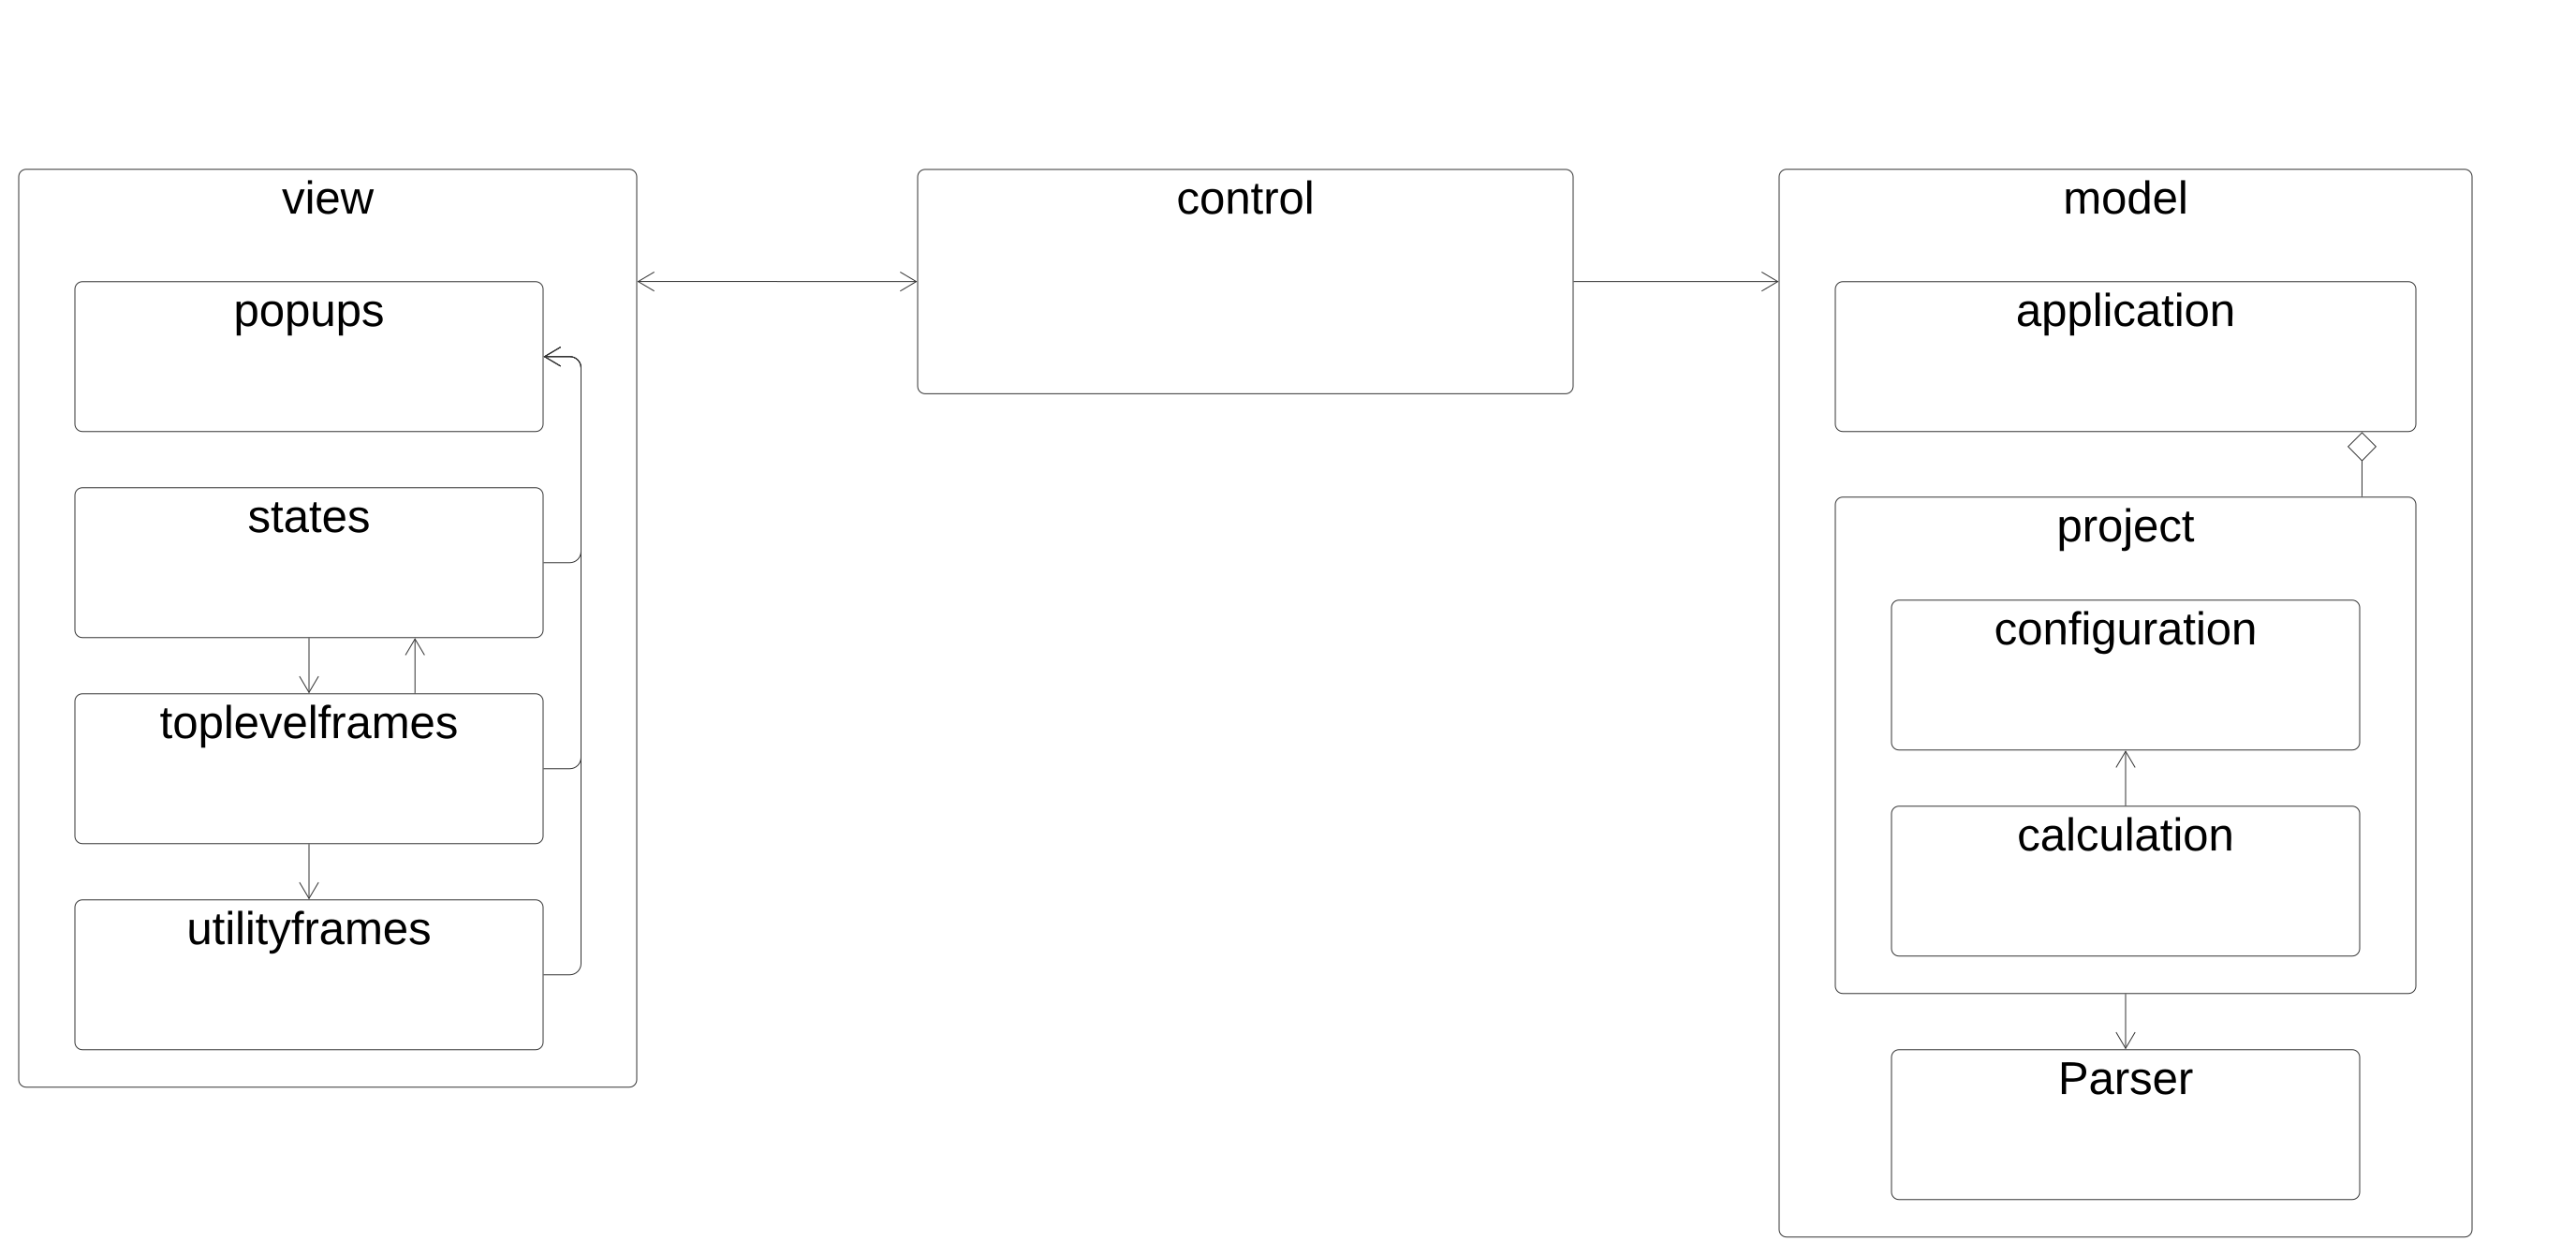
\includegraphics[width=0.8\textwidth]
        {pictures/mvc.png}
  \caption{Model-View-Control Packages}
  \label{fig:mvc}
\end{figure}
}

\hypertarget{controller}{
\begin{figure}[hbt!]
  \centering
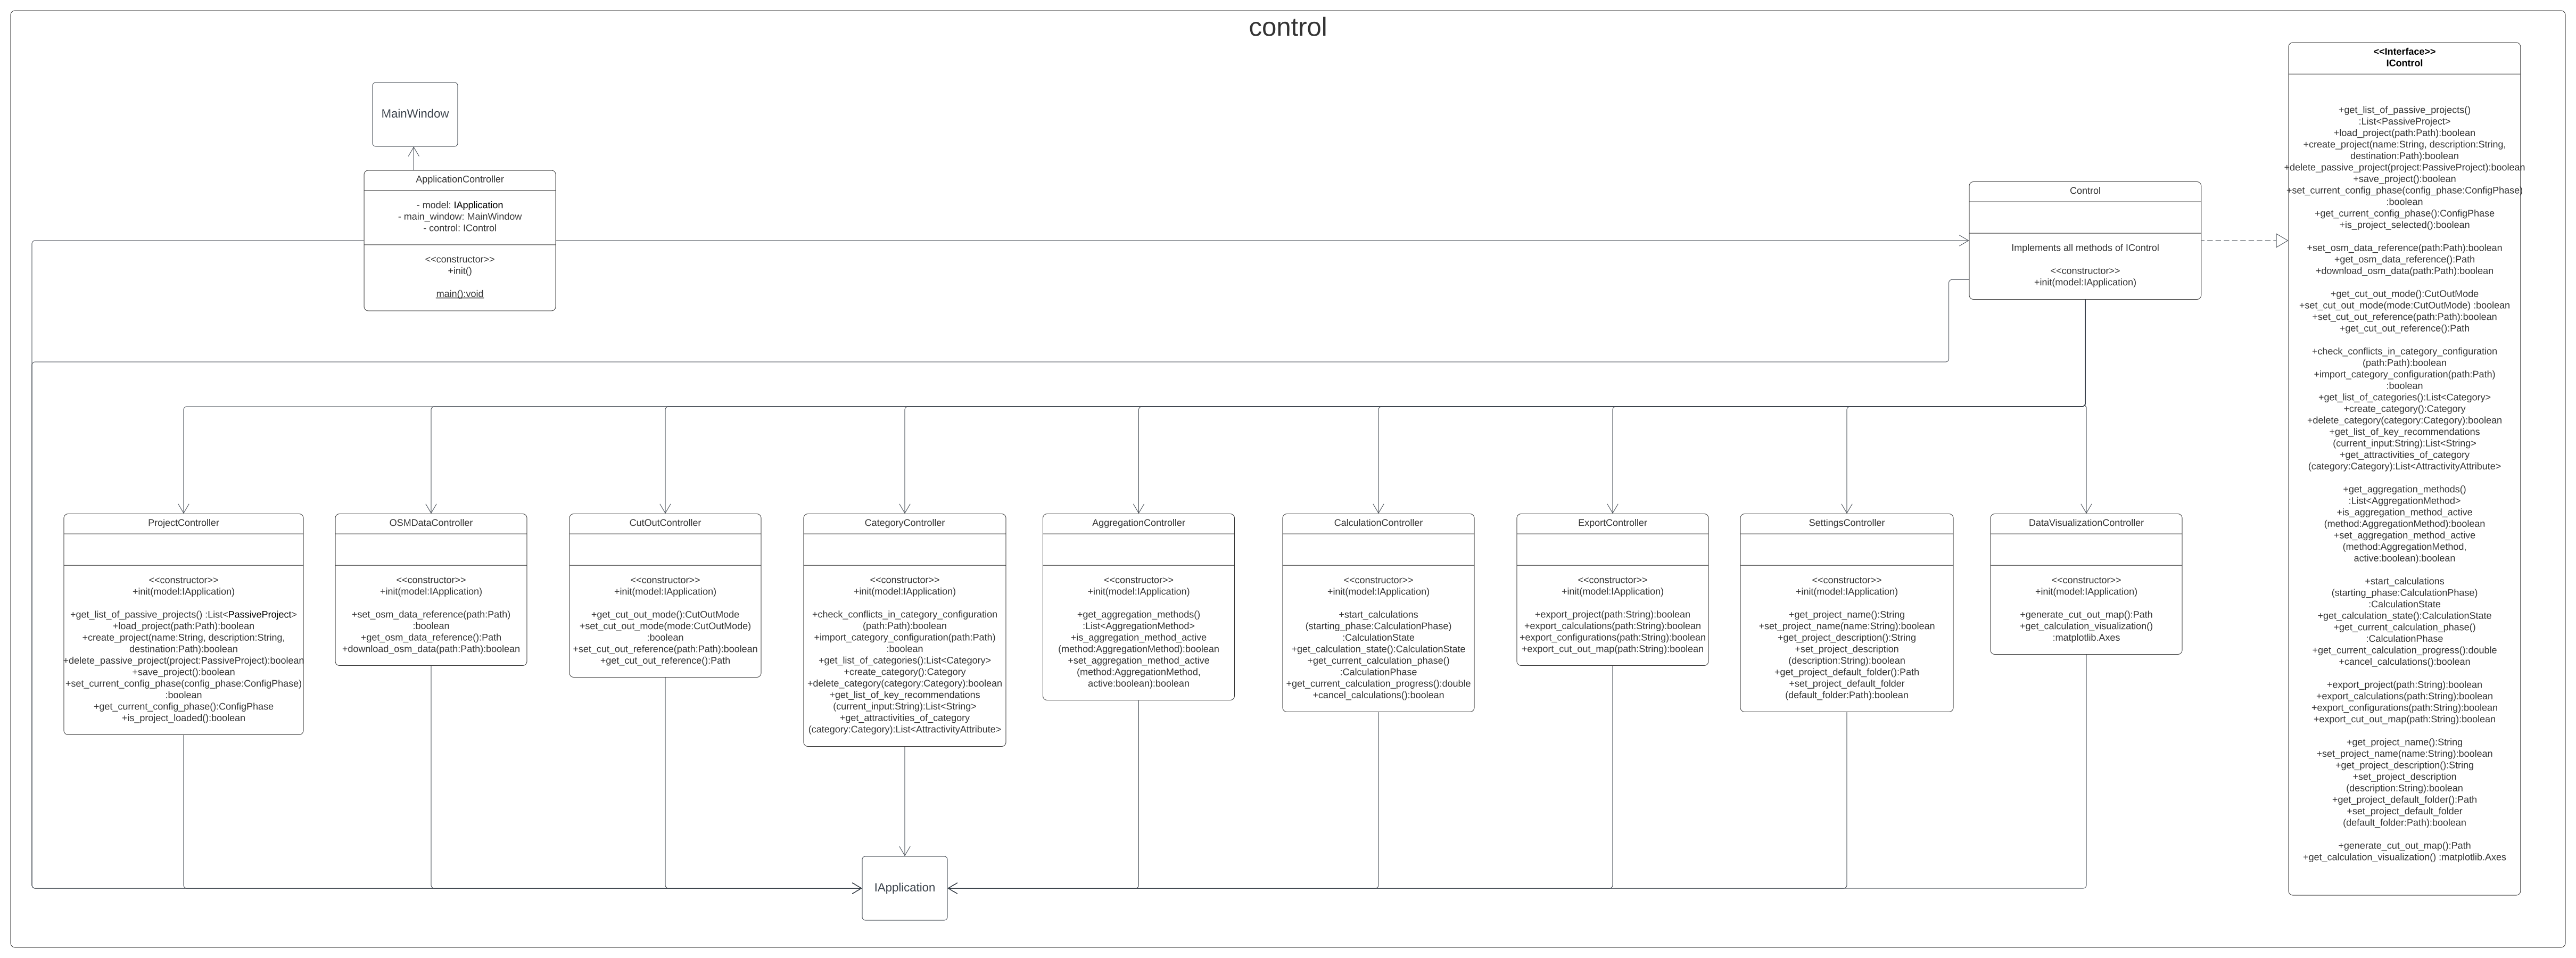
\includegraphics[width=0.8\textwidth]
        {pictures/controller.png}
  \caption{Package: controller}
  \label{fig:controller}
\end{figure}
}

\hypertarget{view}{
\begin{figure}[hbt!]
  \centering
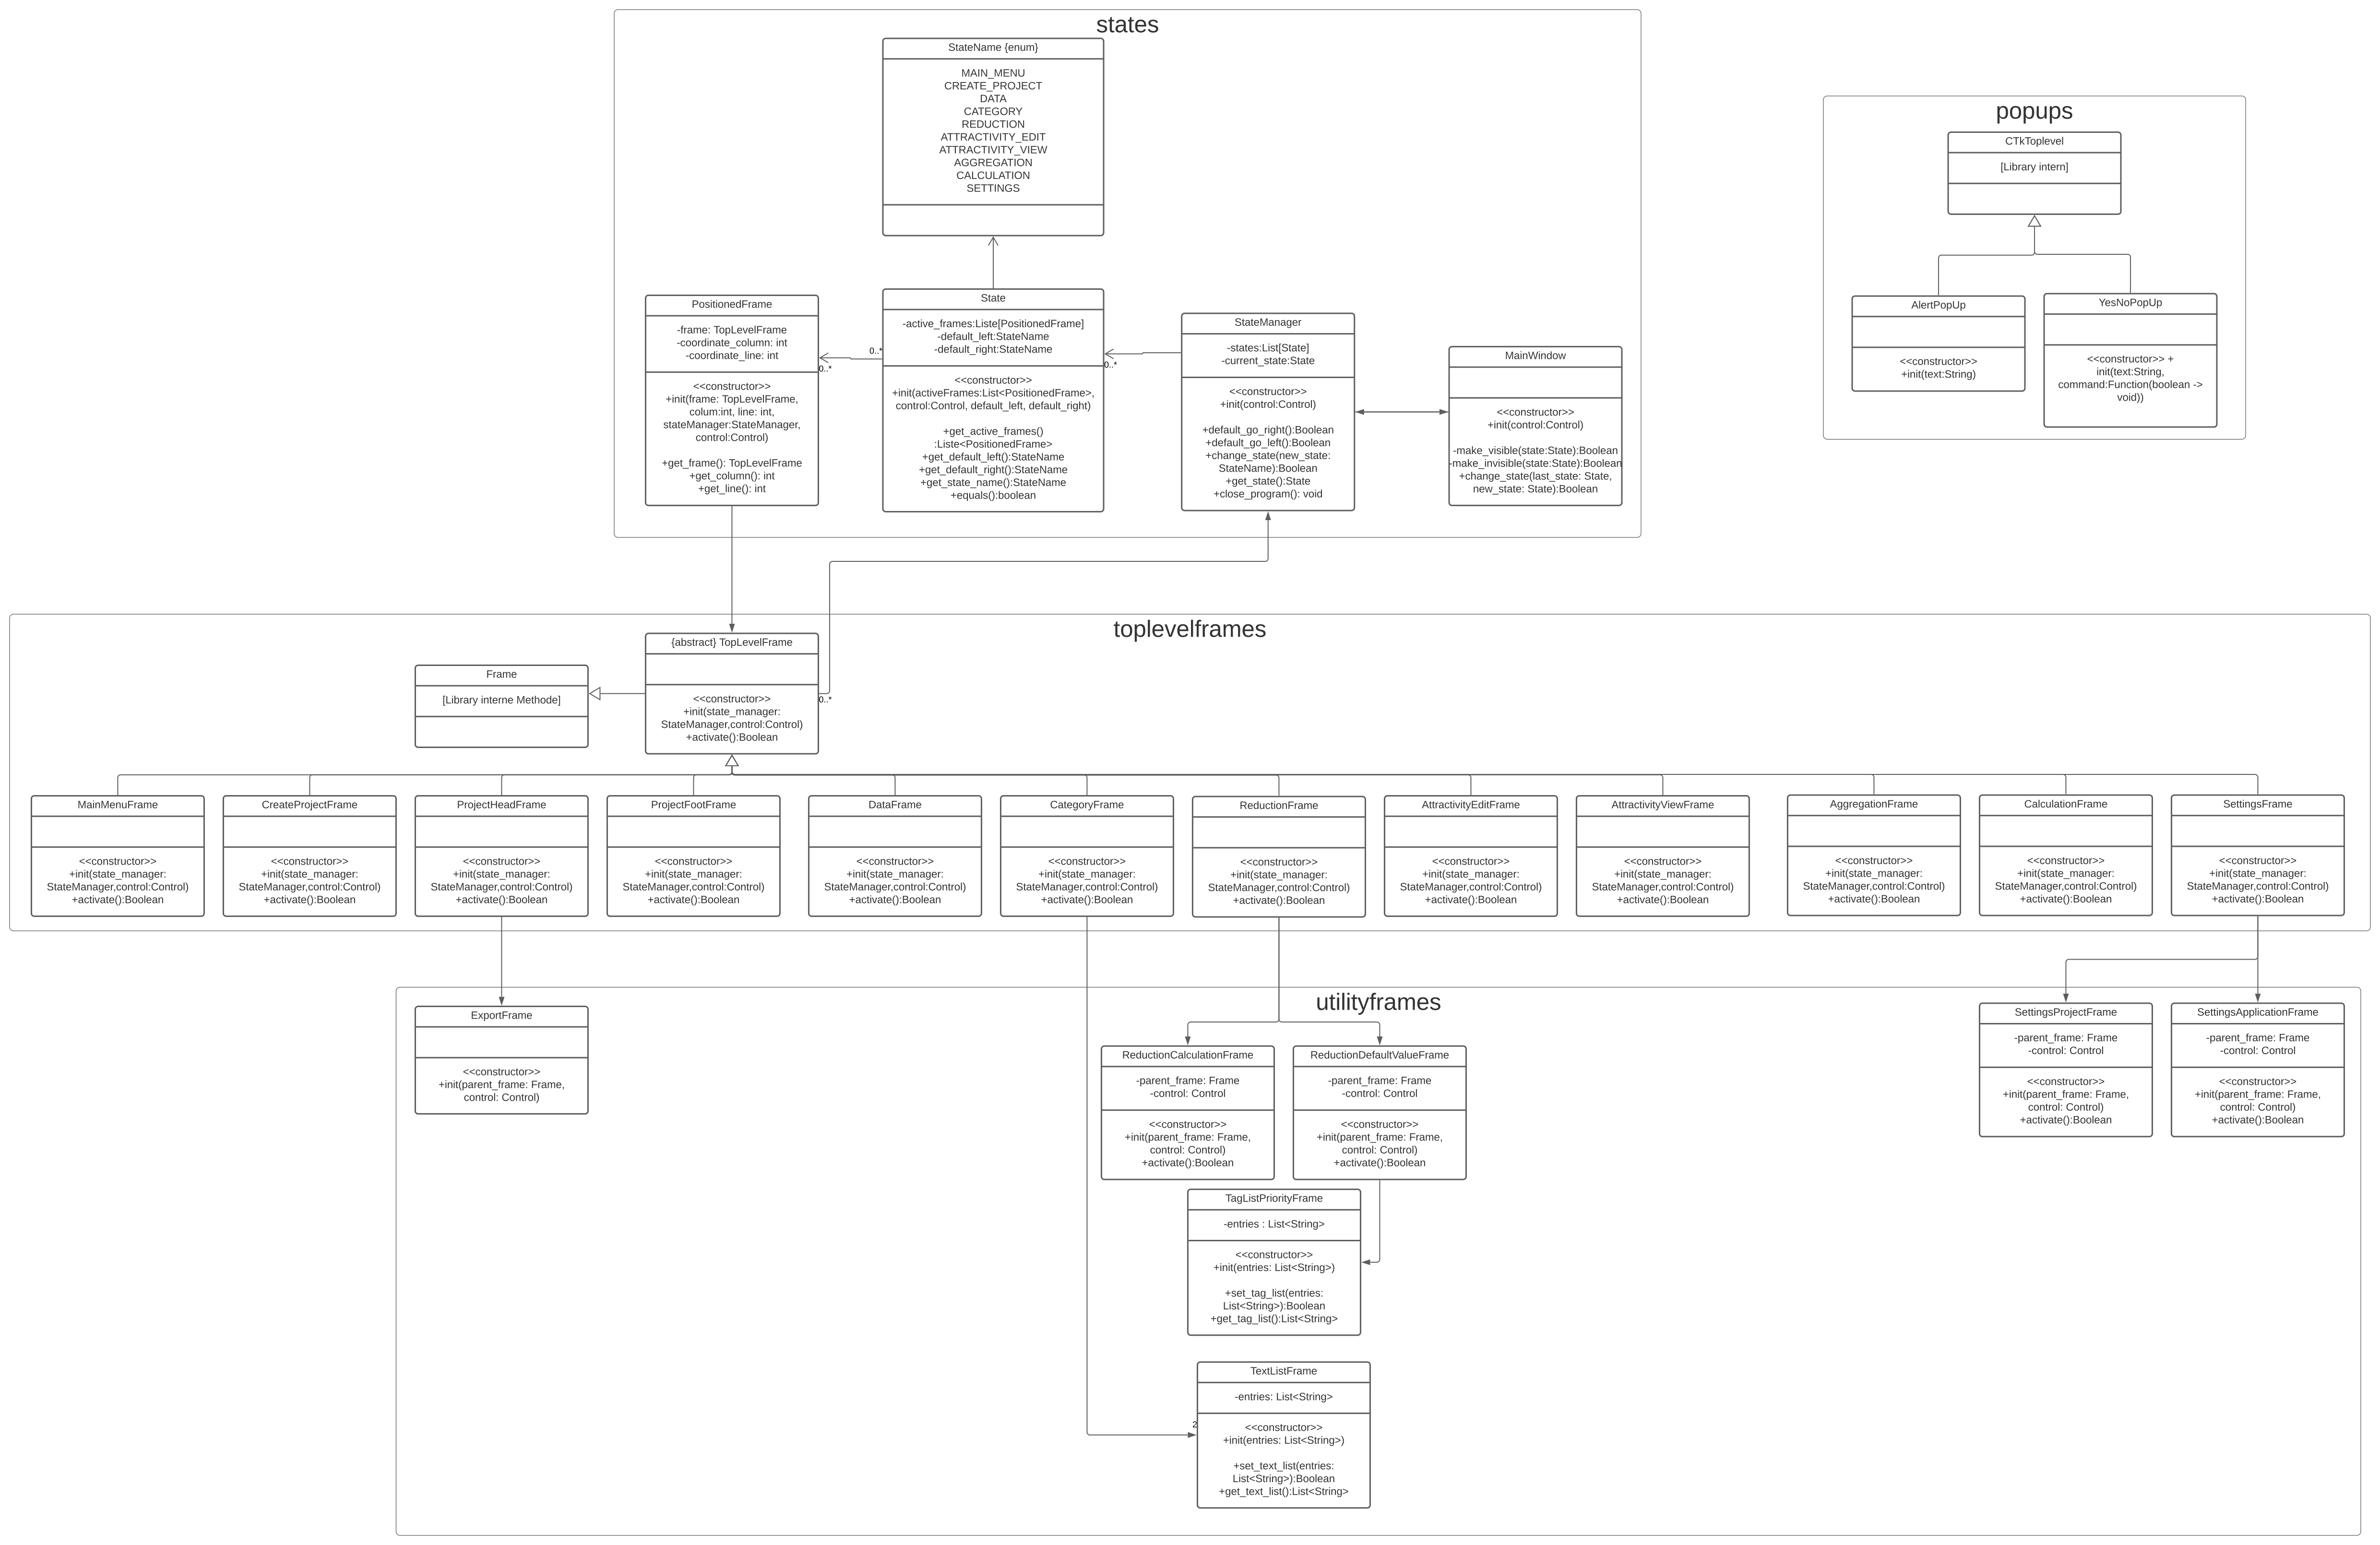
\includegraphics[width=0.8\textwidth]
        {pictures/view.png}
  \caption{Package: view}
  \label{fig:view}
\end{figure}
}

\hypertarget{model}{
\begin{figure}[hbt!]
  \centering
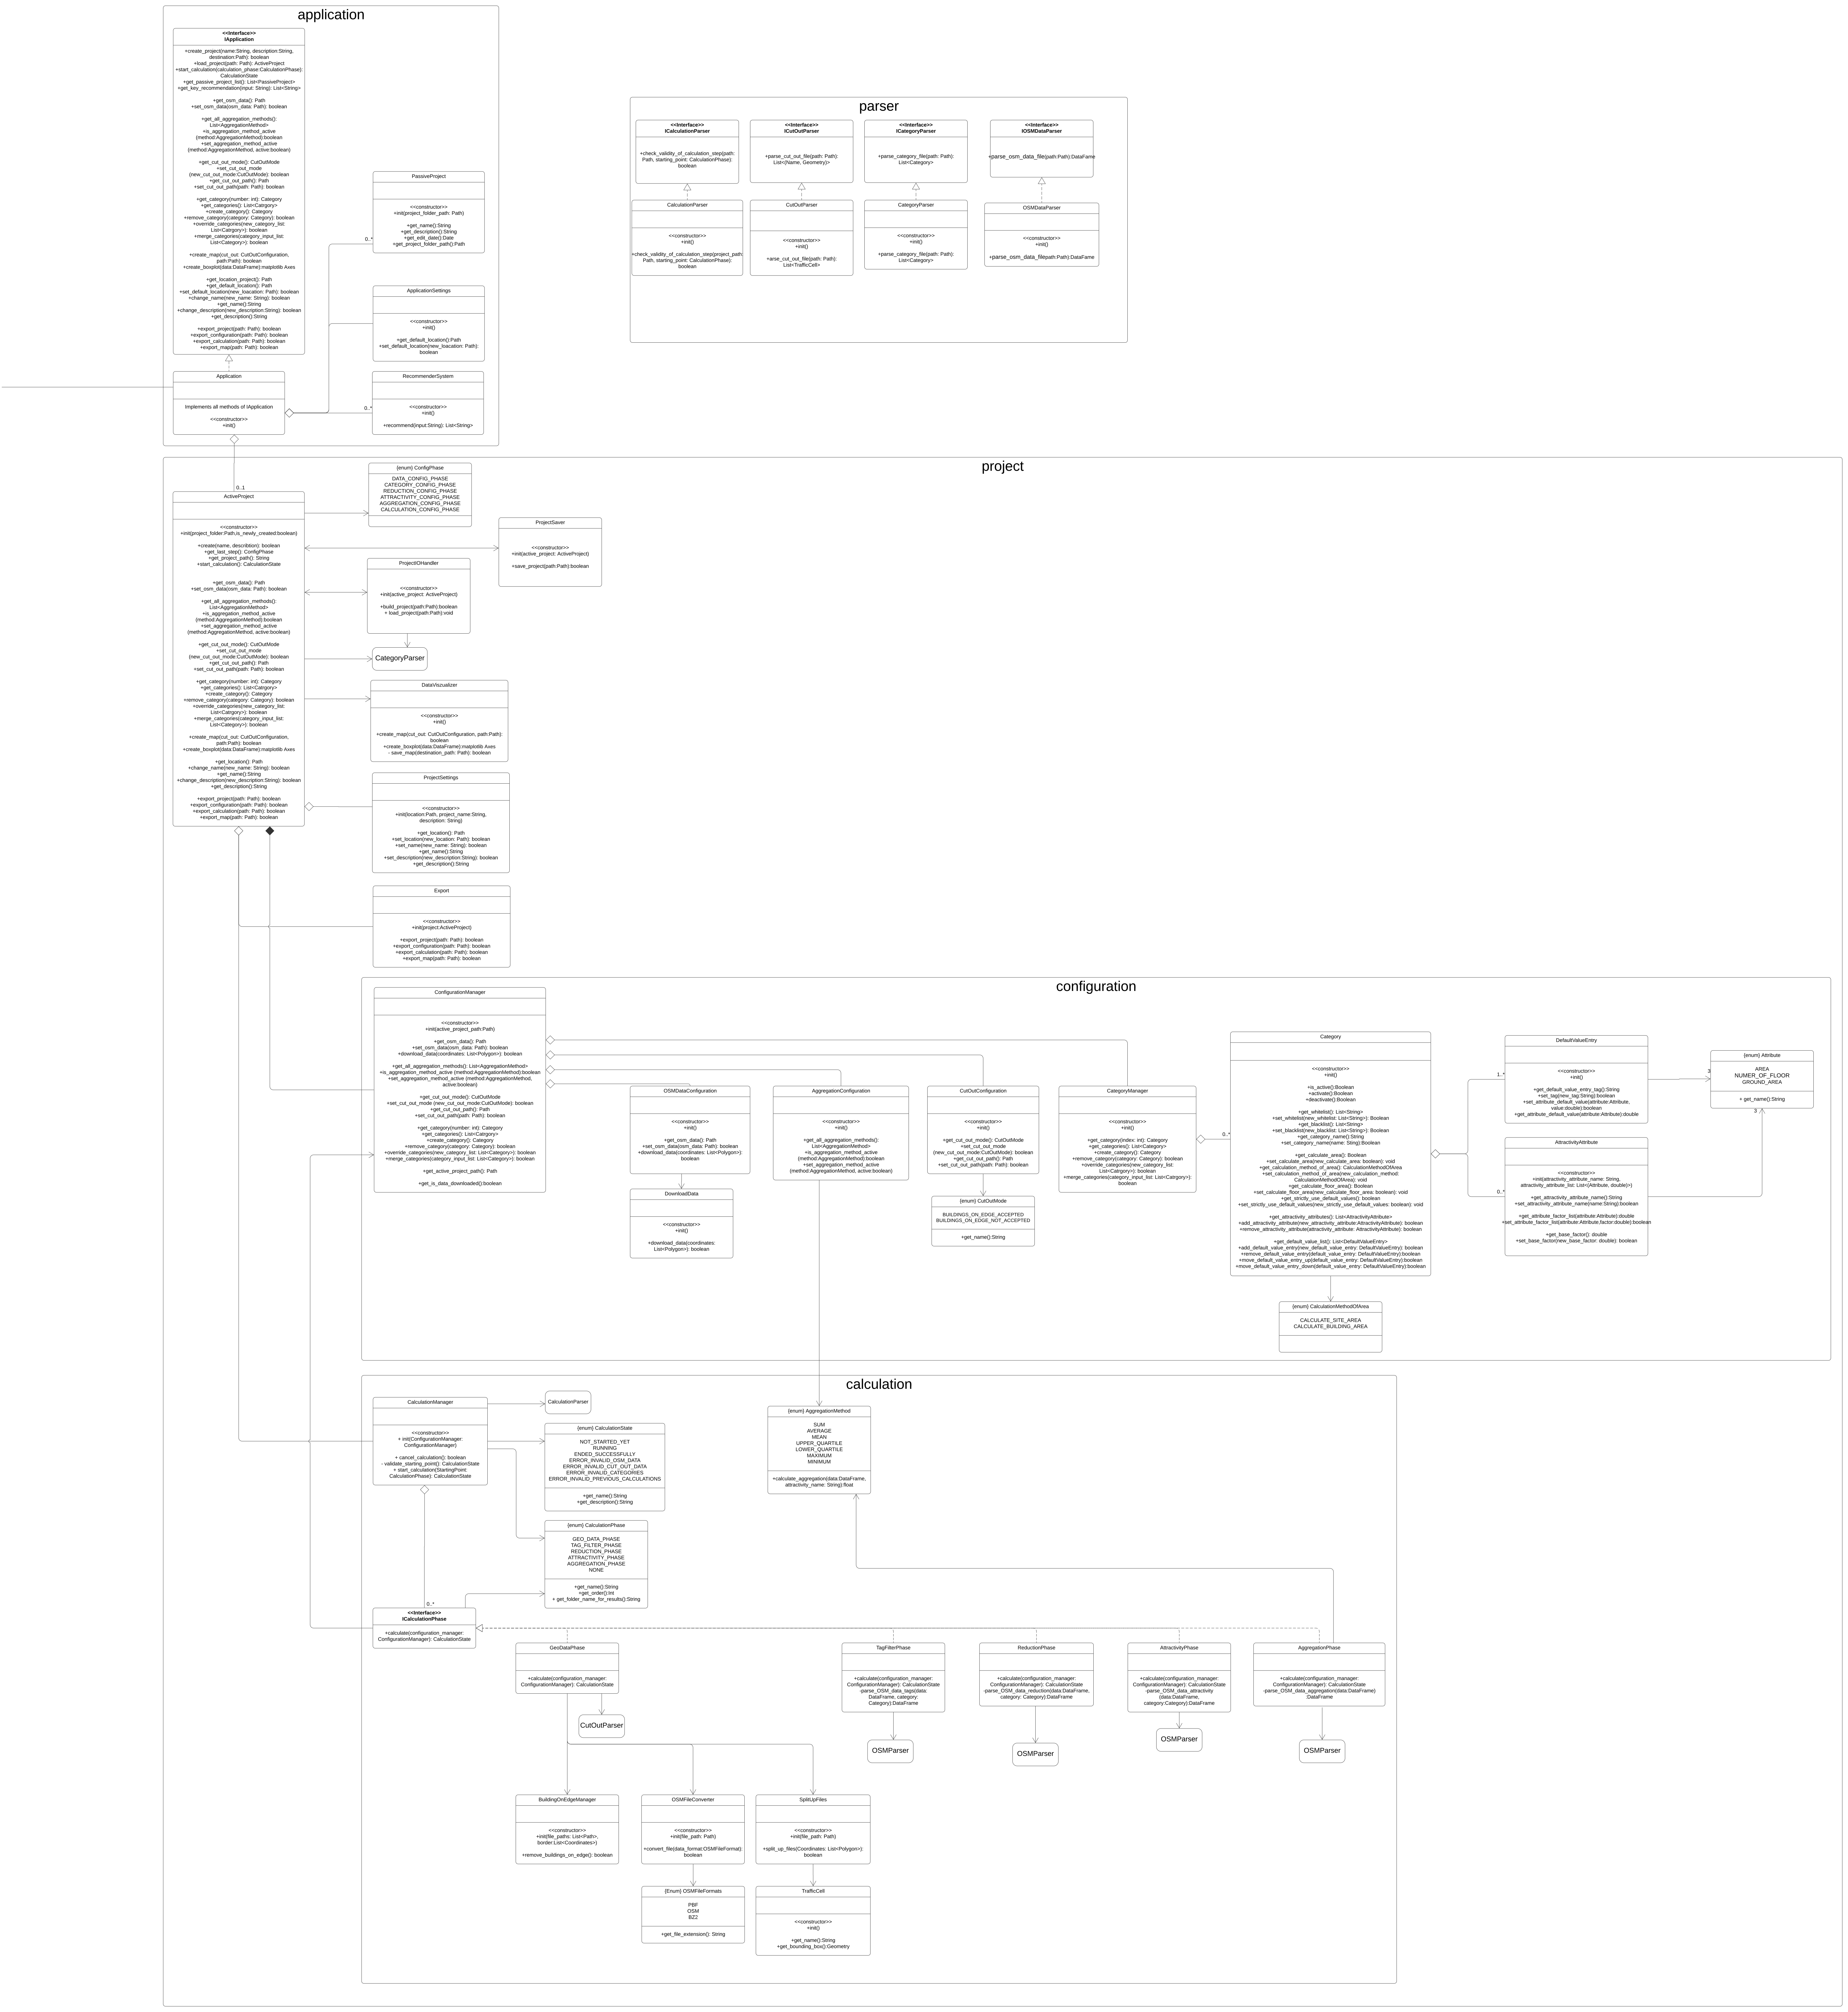
\includegraphics[width=0.8\textwidth]
        {pictures/model.png}
  \caption{Package: model}
  \label{fig:model}
\end{figure}
}

\hypertarget{popups}{
\begin{figure}[hbt!]
  \centering
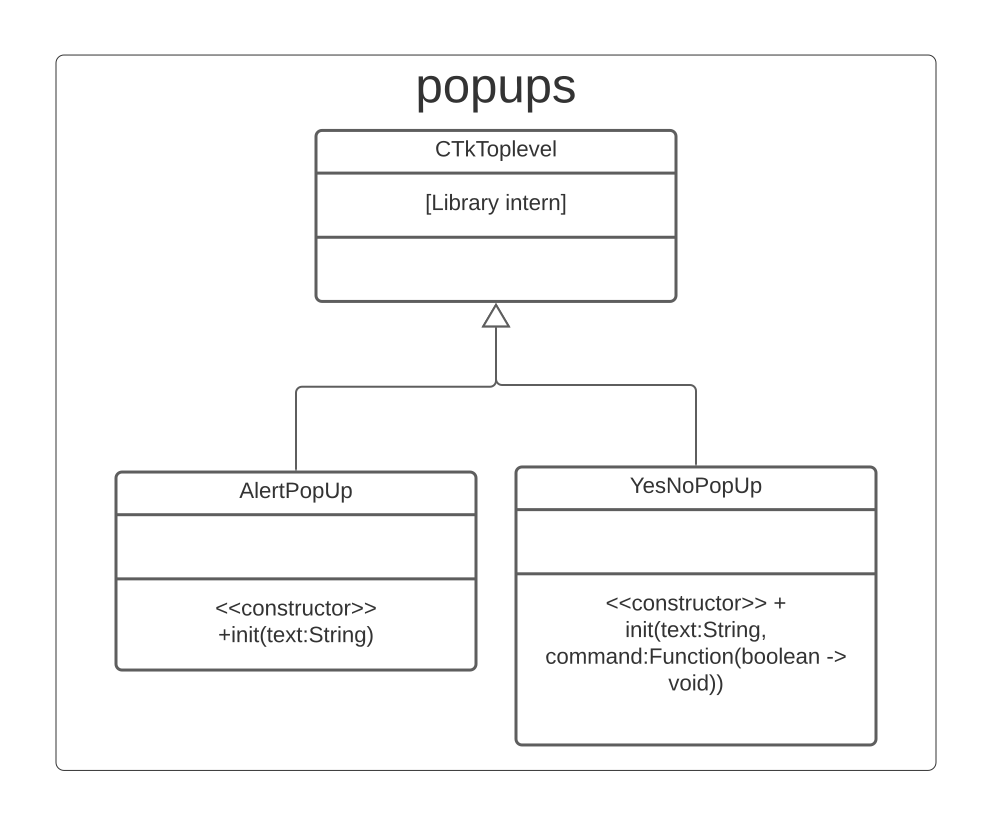
\includegraphics[width=0.5\textwidth]
        {pictures/popups.png}
  \caption{Package: popups}
  \label{fig:popups}
\end{figure}
}

\hypertarget{states}{
\begin{figure}[hbt!]
  \centering
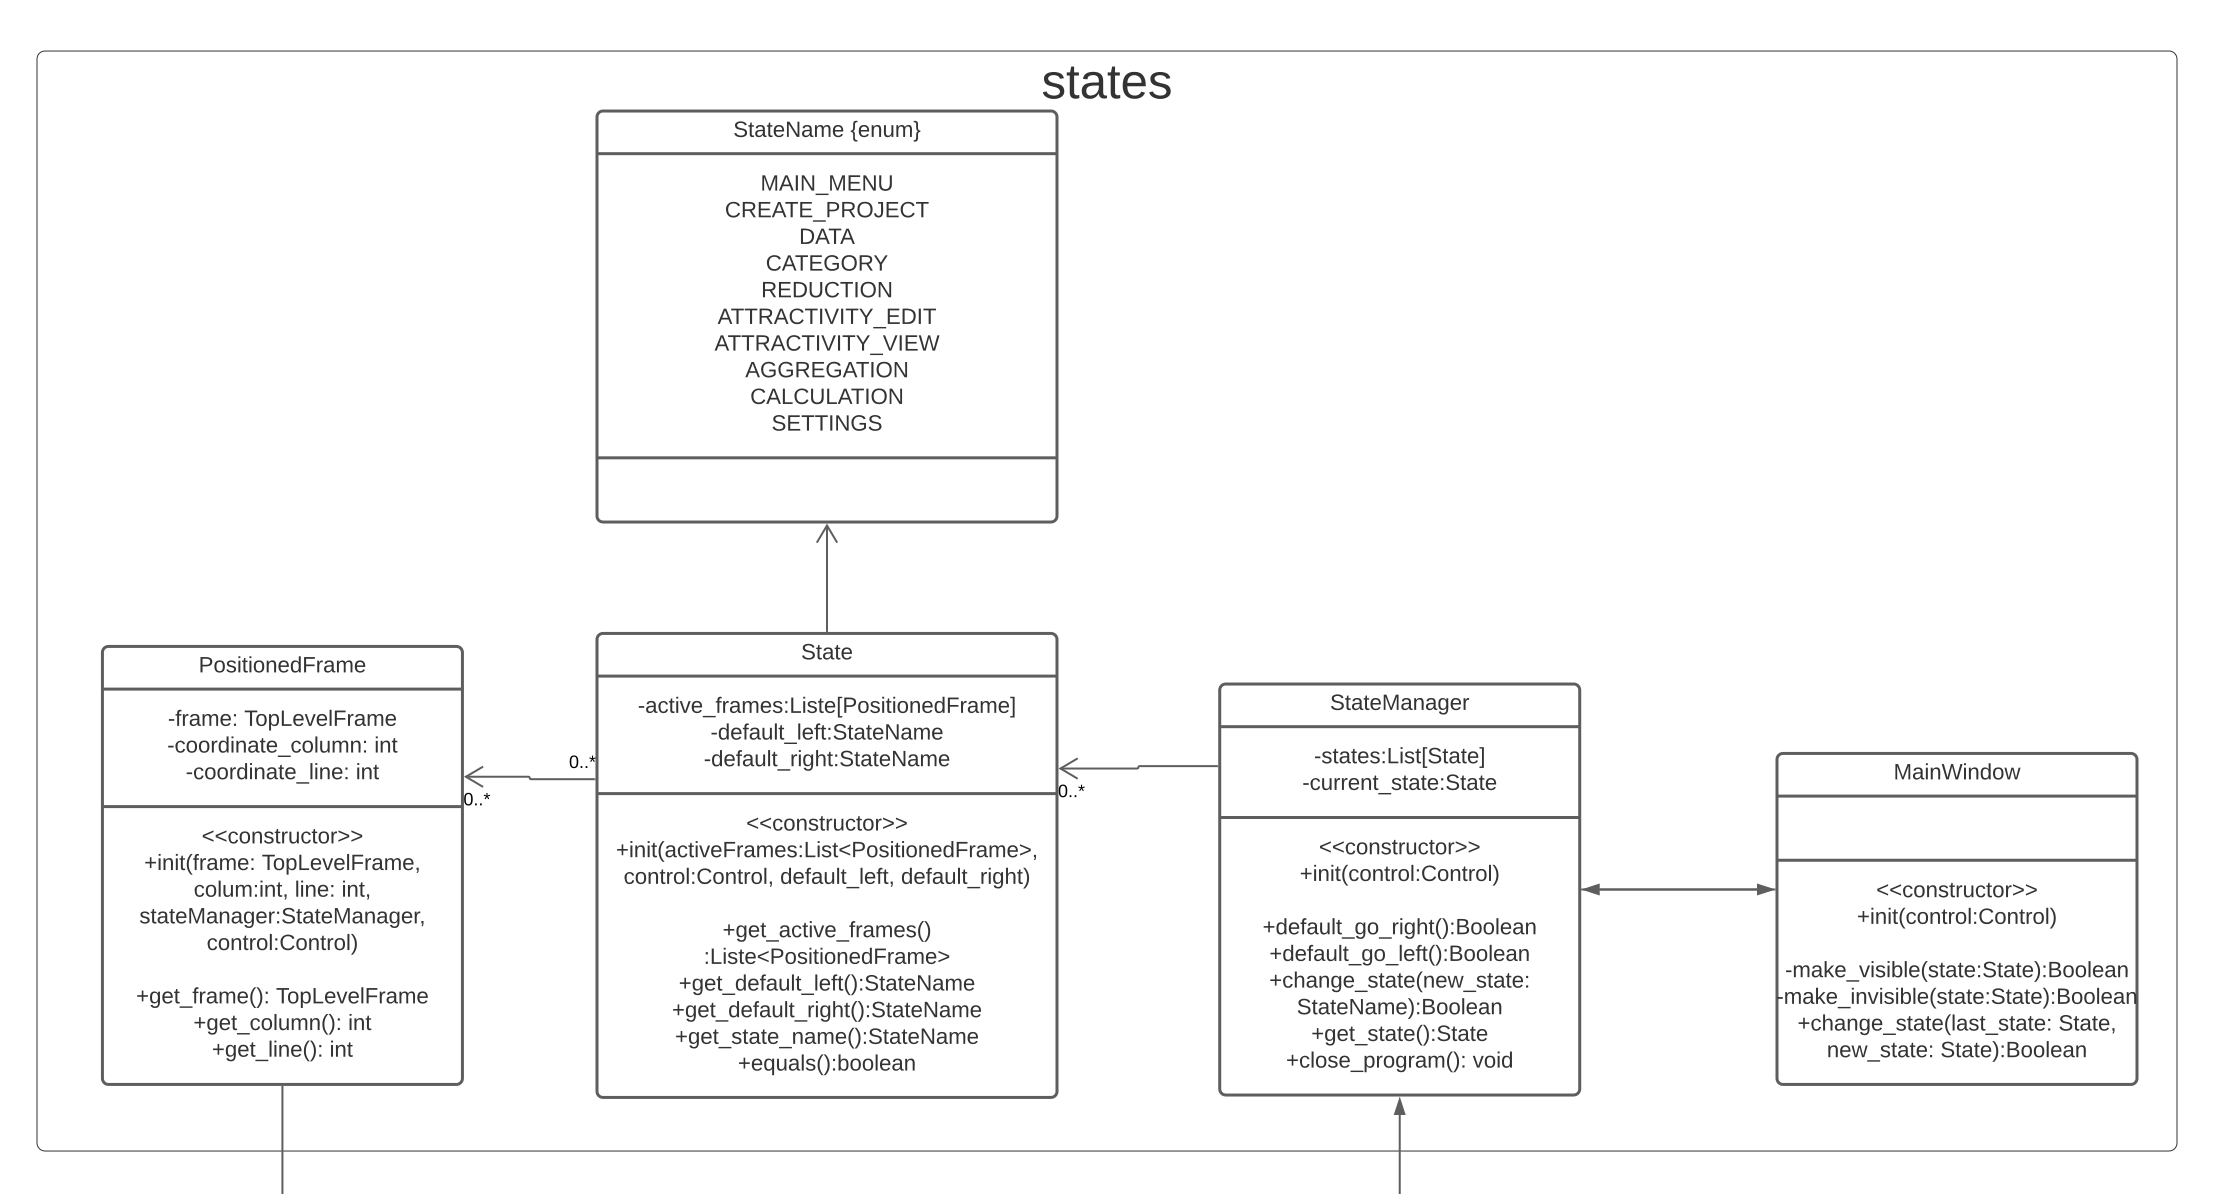
\includegraphics[width=0.8\textwidth]
        {pictures/states.png}
  \caption{Package: states}
  \label{fig:states}
\end{figure}
}

\hypertarget{toplevelframes}{
\begin{figure}[hbt!]
  \centering
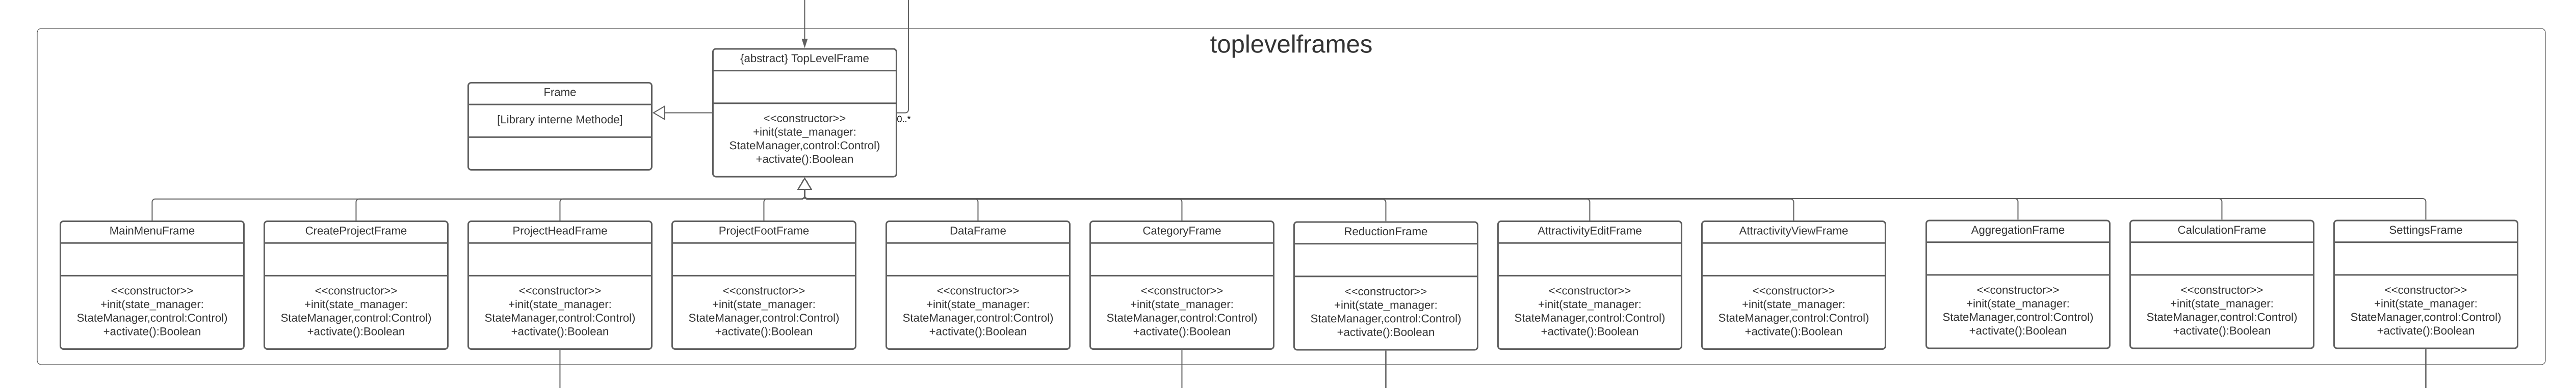
\includegraphics[width=0.8\textwidth]
        {pictures/toplevelframes.png}
  \caption{Package: toplevelframes}
  \label{fig:toplevelframes}
\end{figure}
}

\hypertarget{utilityframes}{
\begin{figure}[hbt!]
  \centering
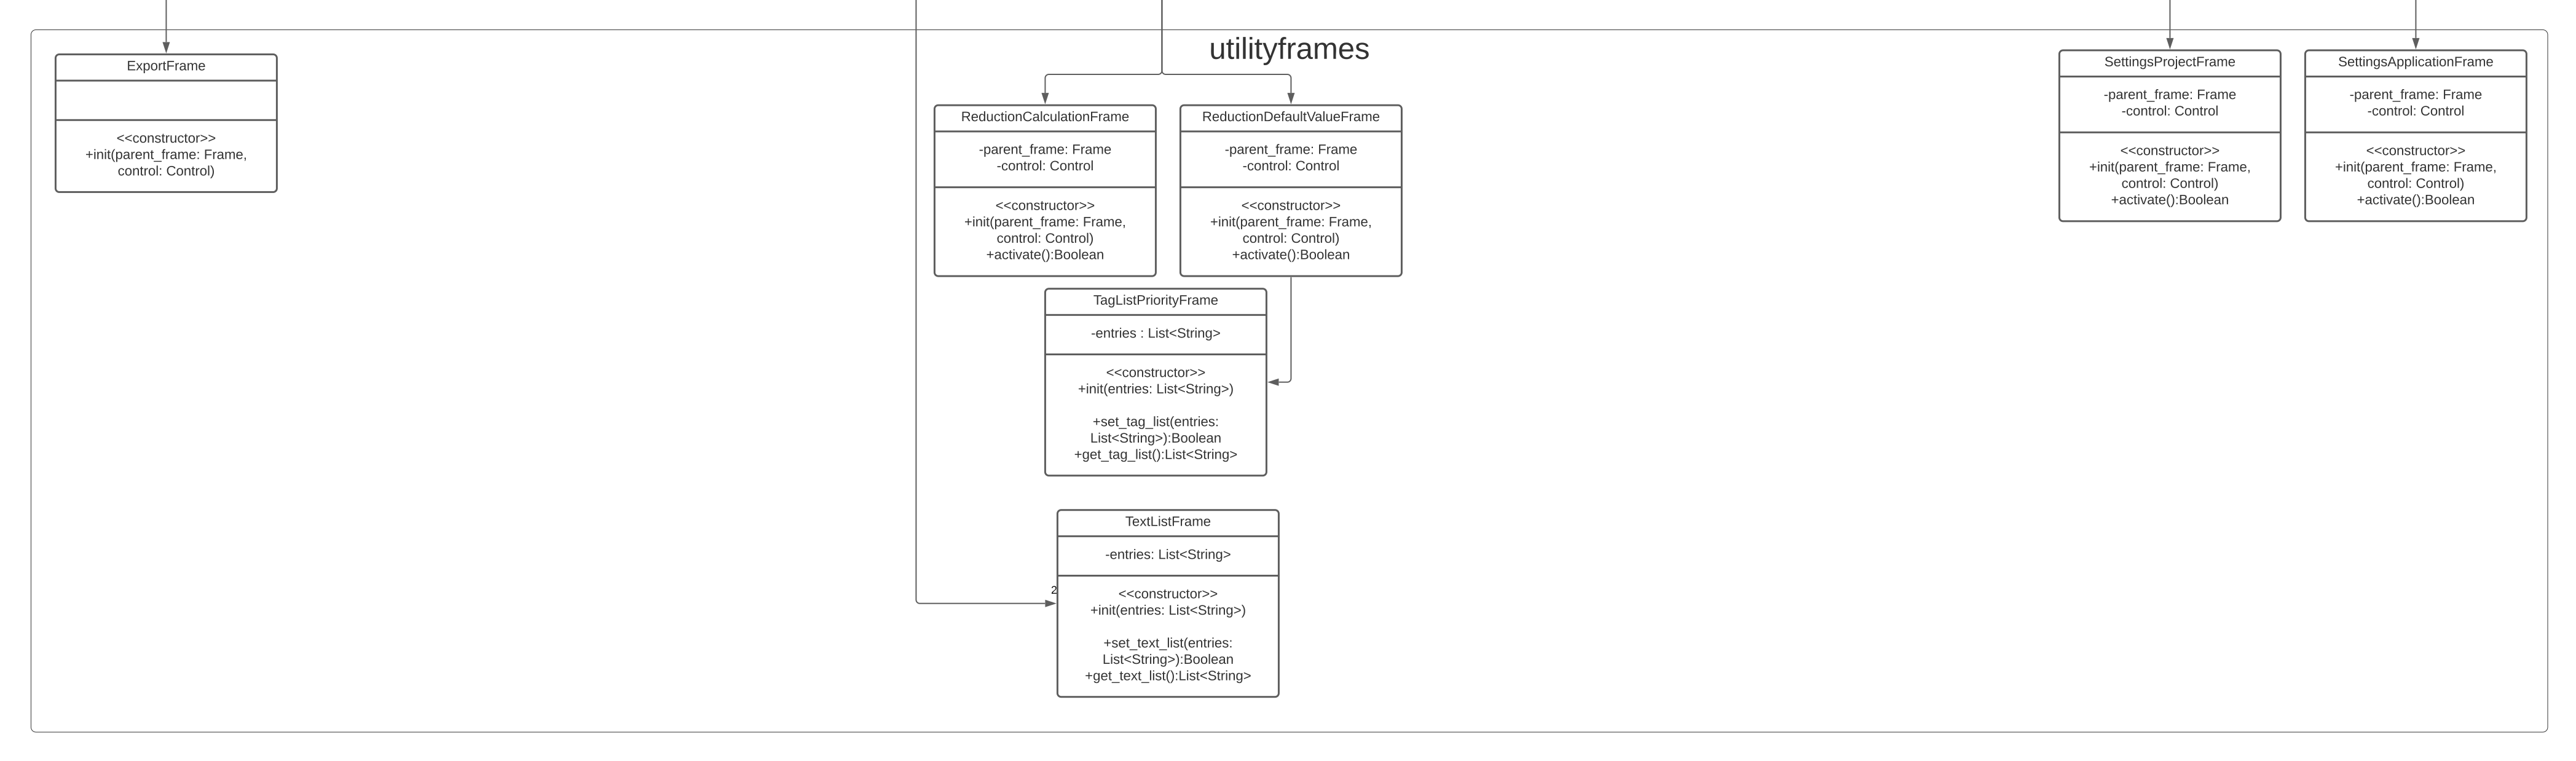
\includegraphics[width=0.8\textwidth]
        {pictures/utilityframes.png}
  \caption{Package: utilityframes}
  \label{fig:utilityframes}
\end{figure}
}

\hypertarget{application}{
\begin{figure}[hbt!]
  \centering
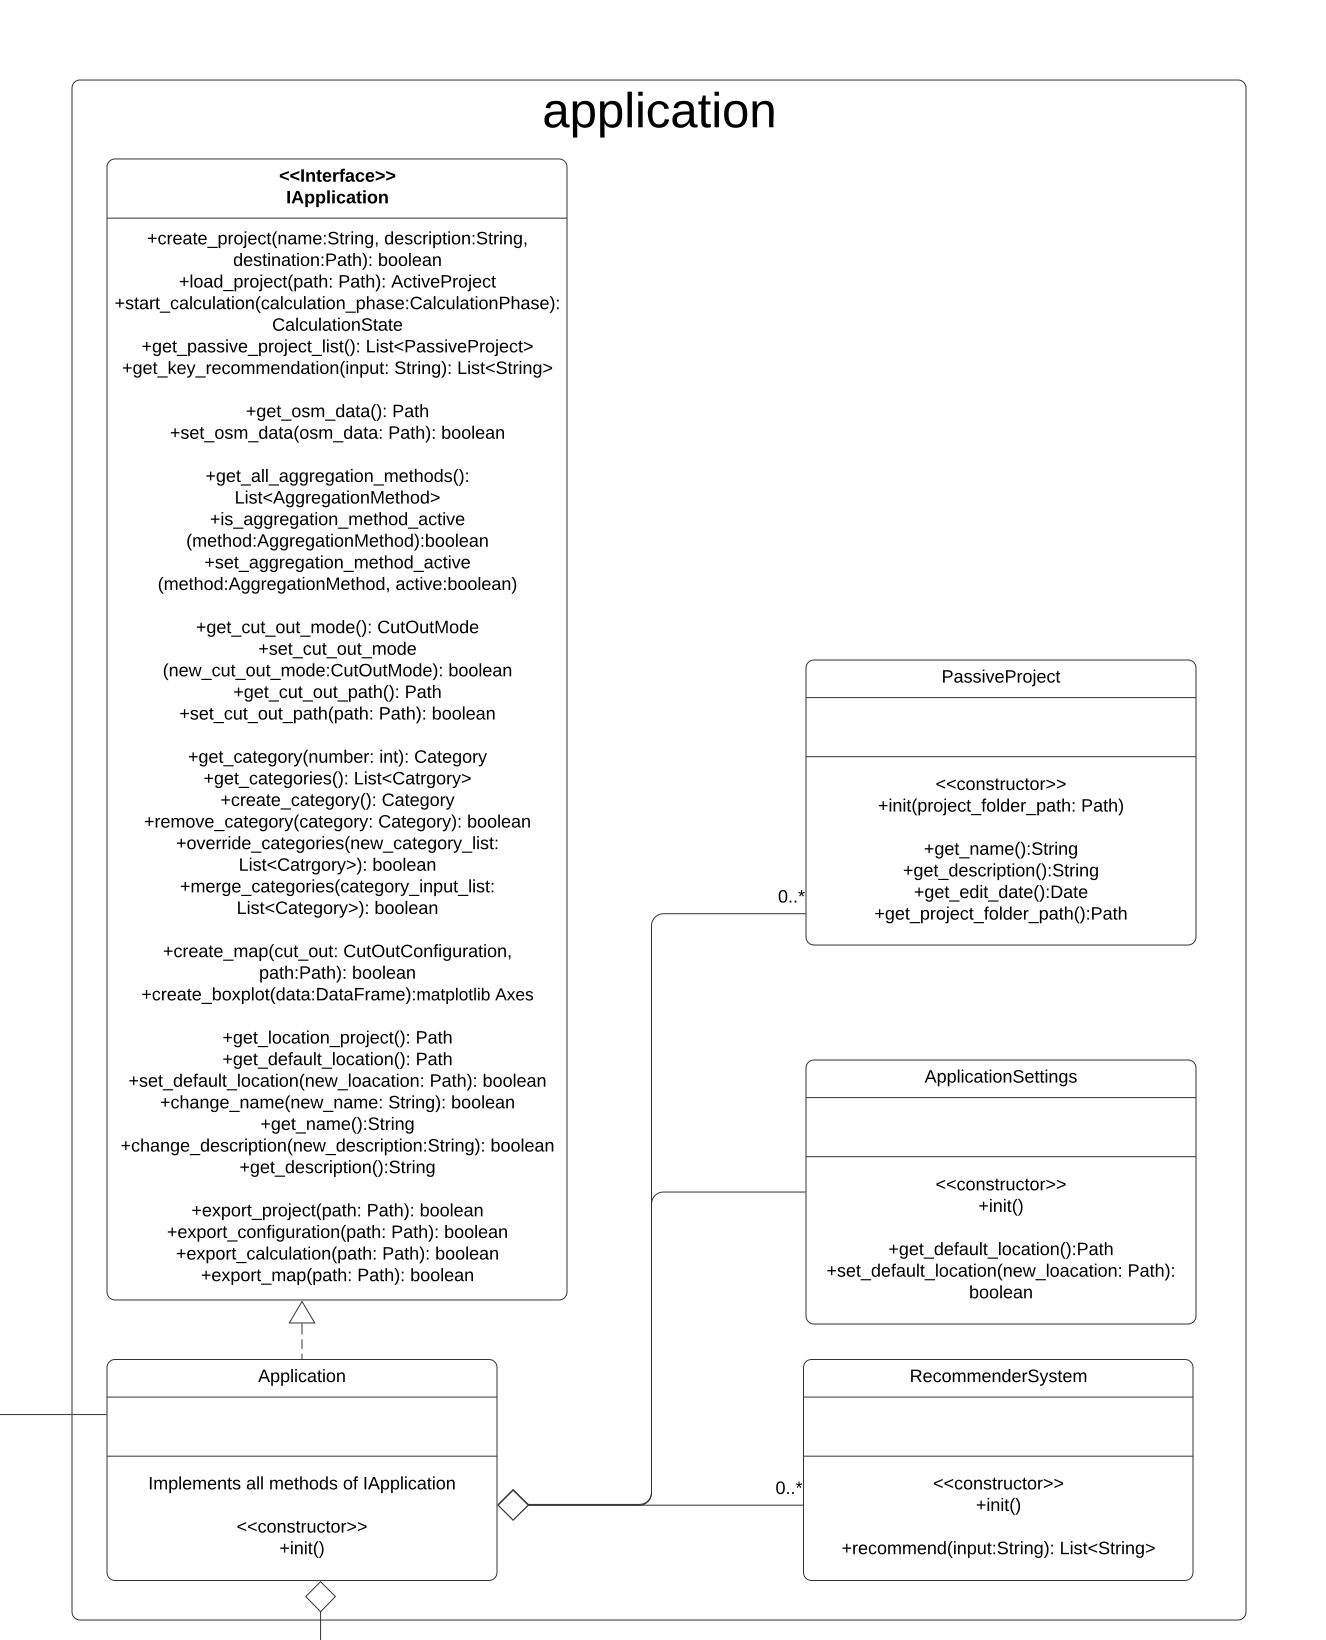
\includegraphics[width=0.8\textwidth]
        {pictures/application.png}
  \caption{Package: application}
  \label{fig:application}
\end{figure}
}

\hypertarget{parser}{
\begin{figure}[hbt!]
  \centering
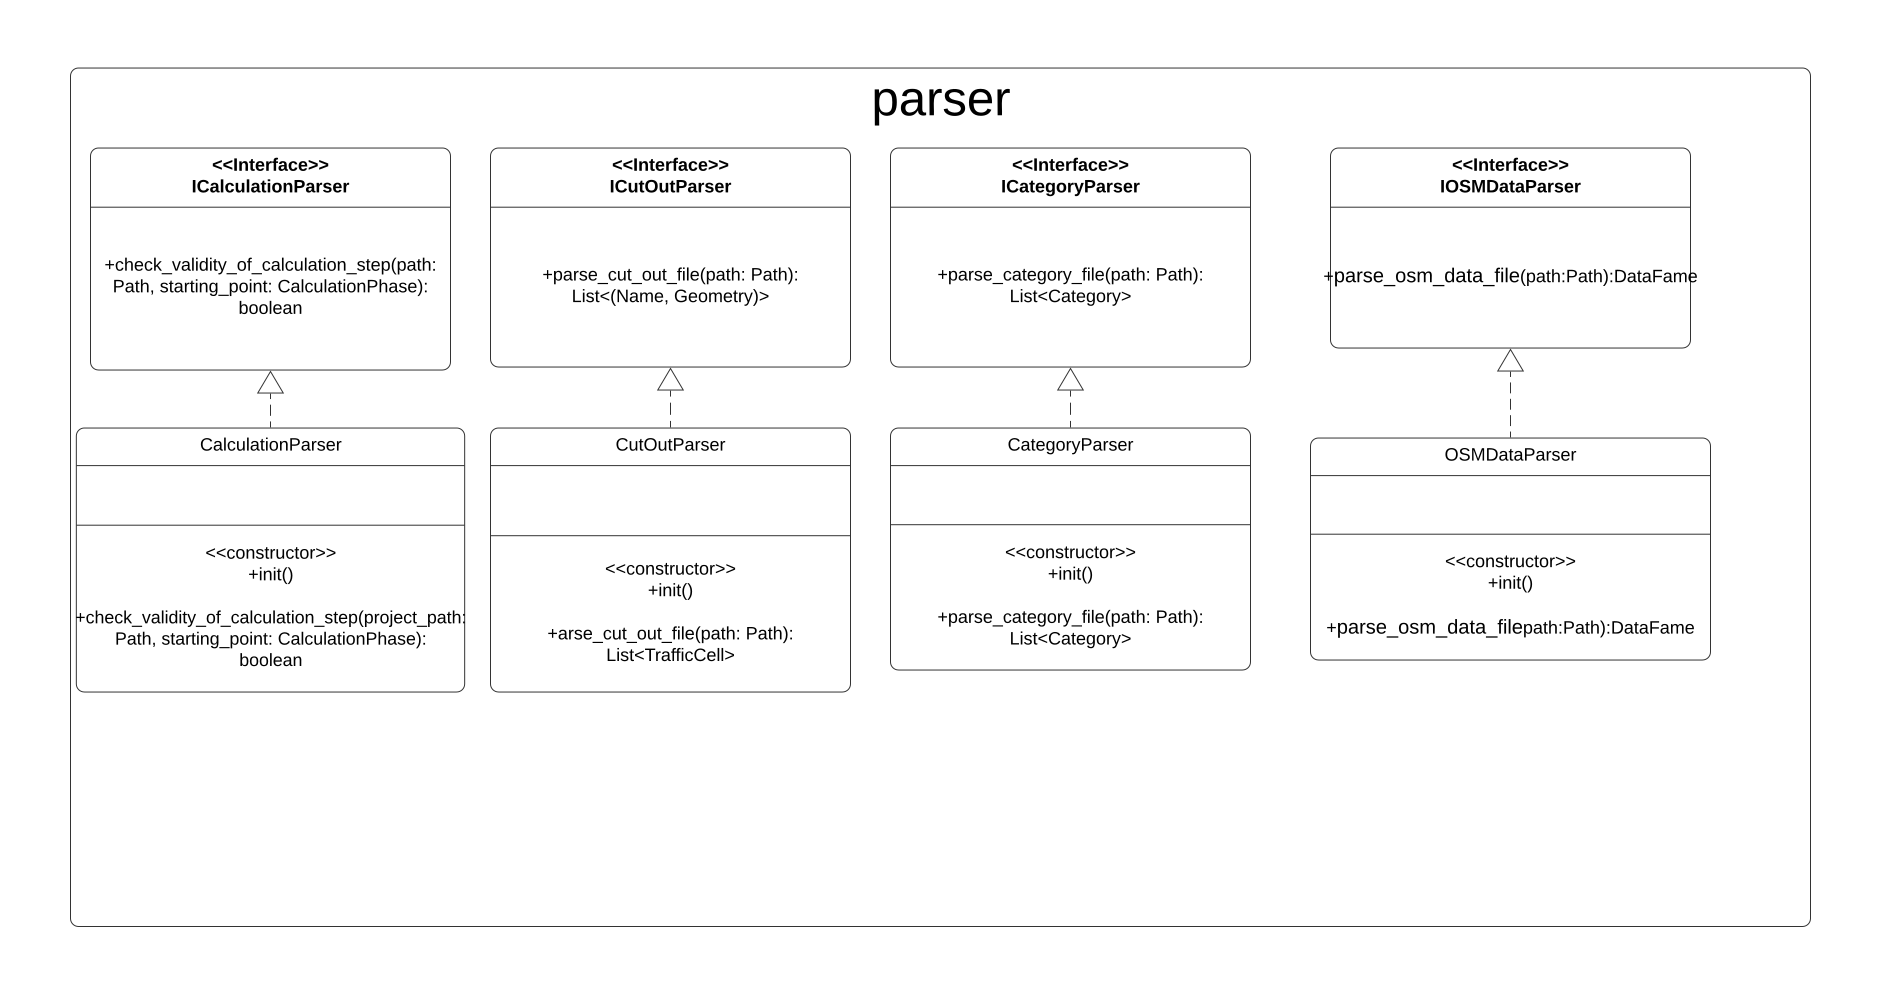
\includegraphics[width=0.7\textwidth]
        {pictures/parser.png}
  \caption{Package: parser}
  \label{fig:parser}
\end{figure}
}

\hypertarget{project}{
\begin{figure}[hbt!]
  \centering
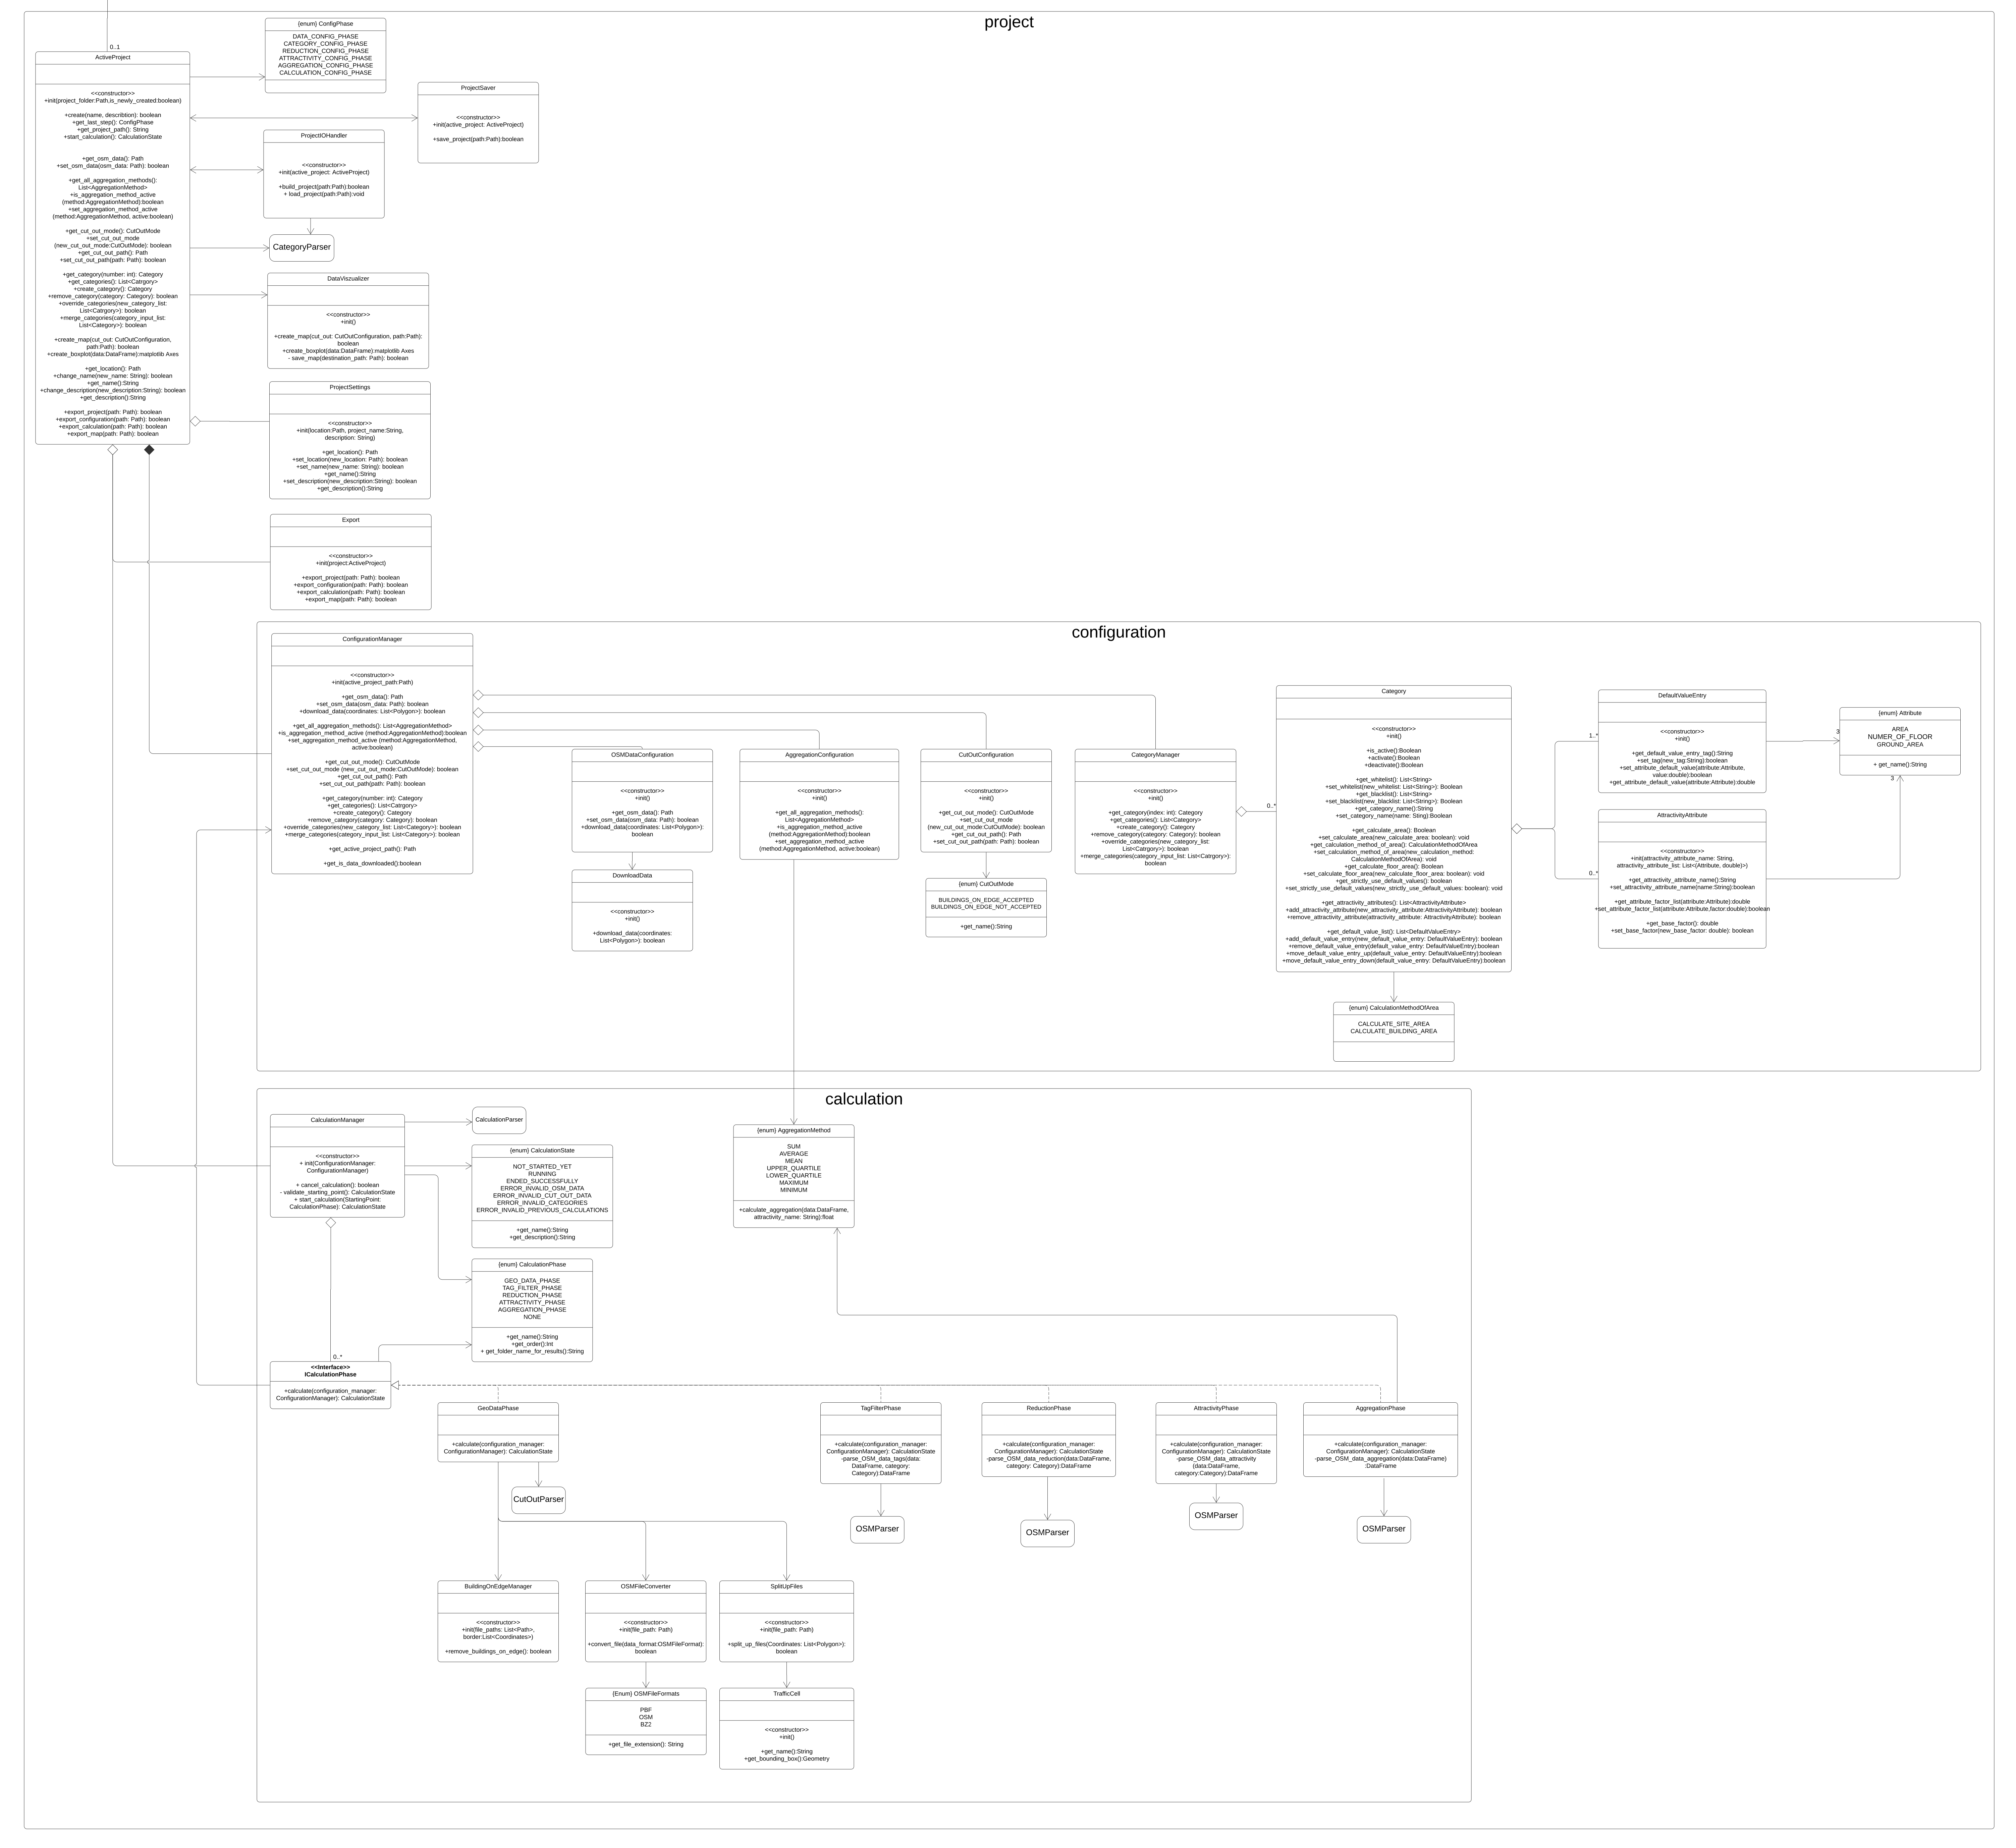
\includegraphics[width=0.8\textwidth]
        {pictures/project.png}
  \caption{Package: project}
  \label{fig:project}
\end{figure}
}

\hypertarget{configuration}{
\begin{figure}[hbt!]
  \centering
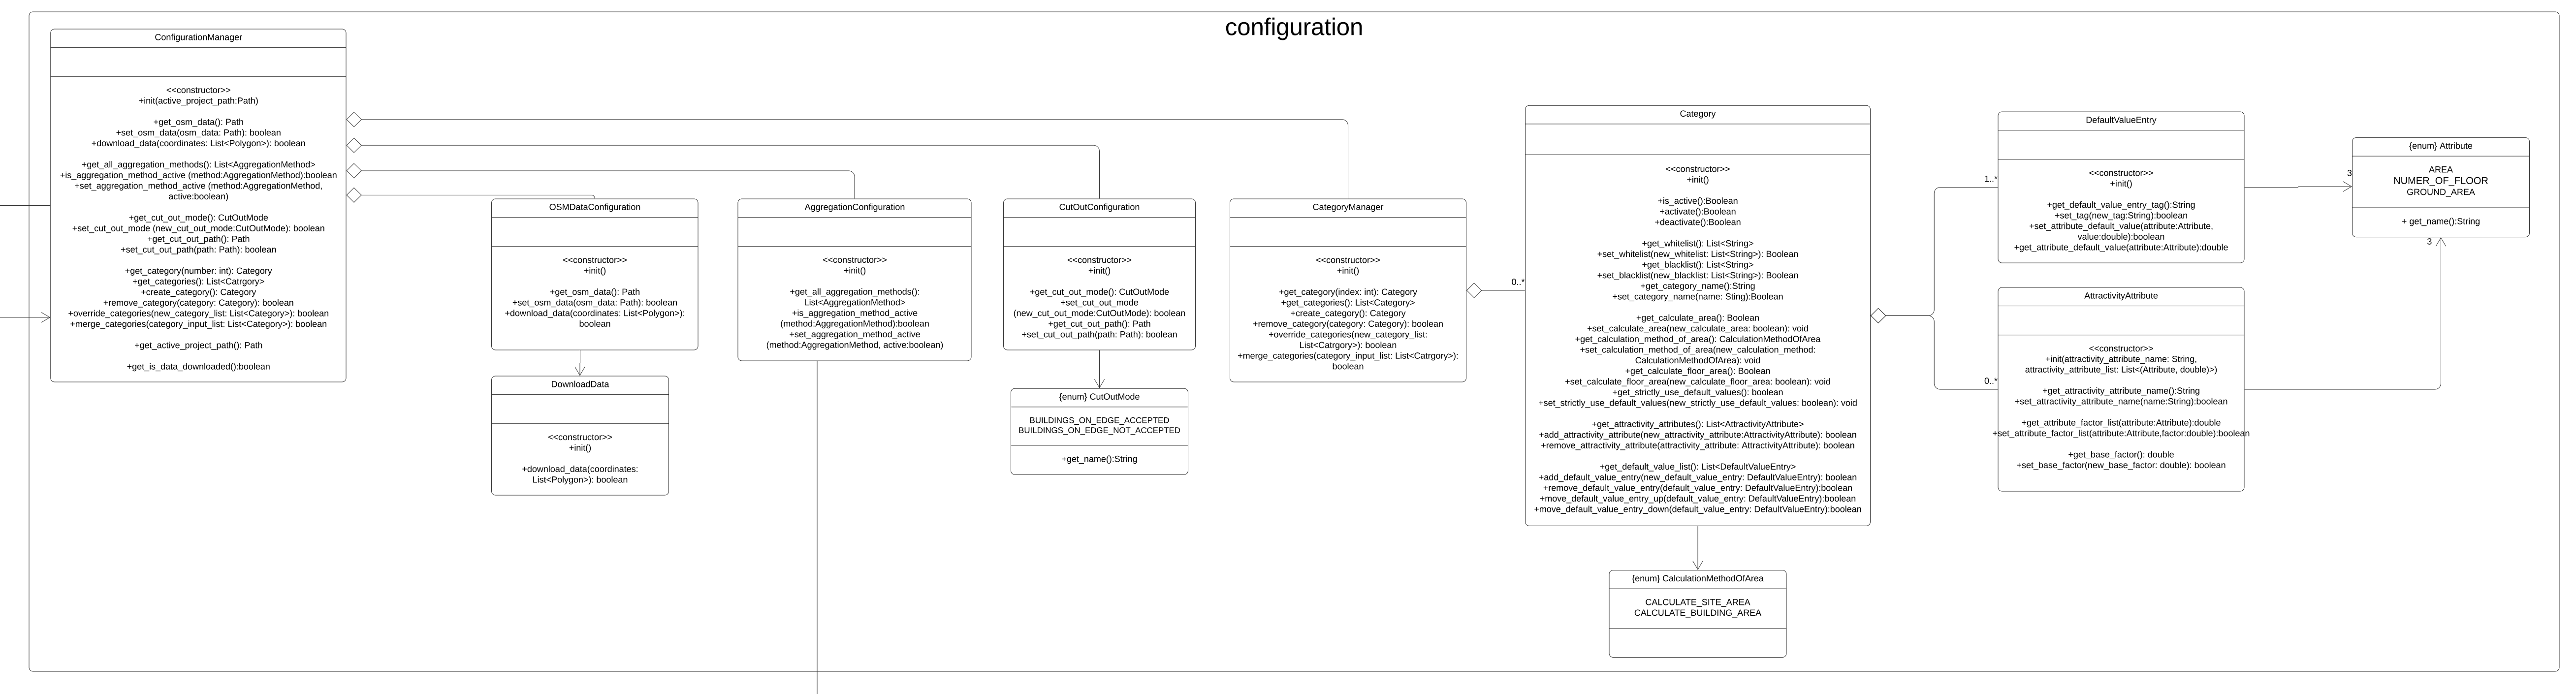
\includegraphics[width=0.8\textwidth]
        {pictures/configuration.png}
  \caption{Package: configuration}
  \label{fig:configuration}
\end{figure}
}

\hypertarget{calculation}{
\begin{figure}[hbt!]
  \centering
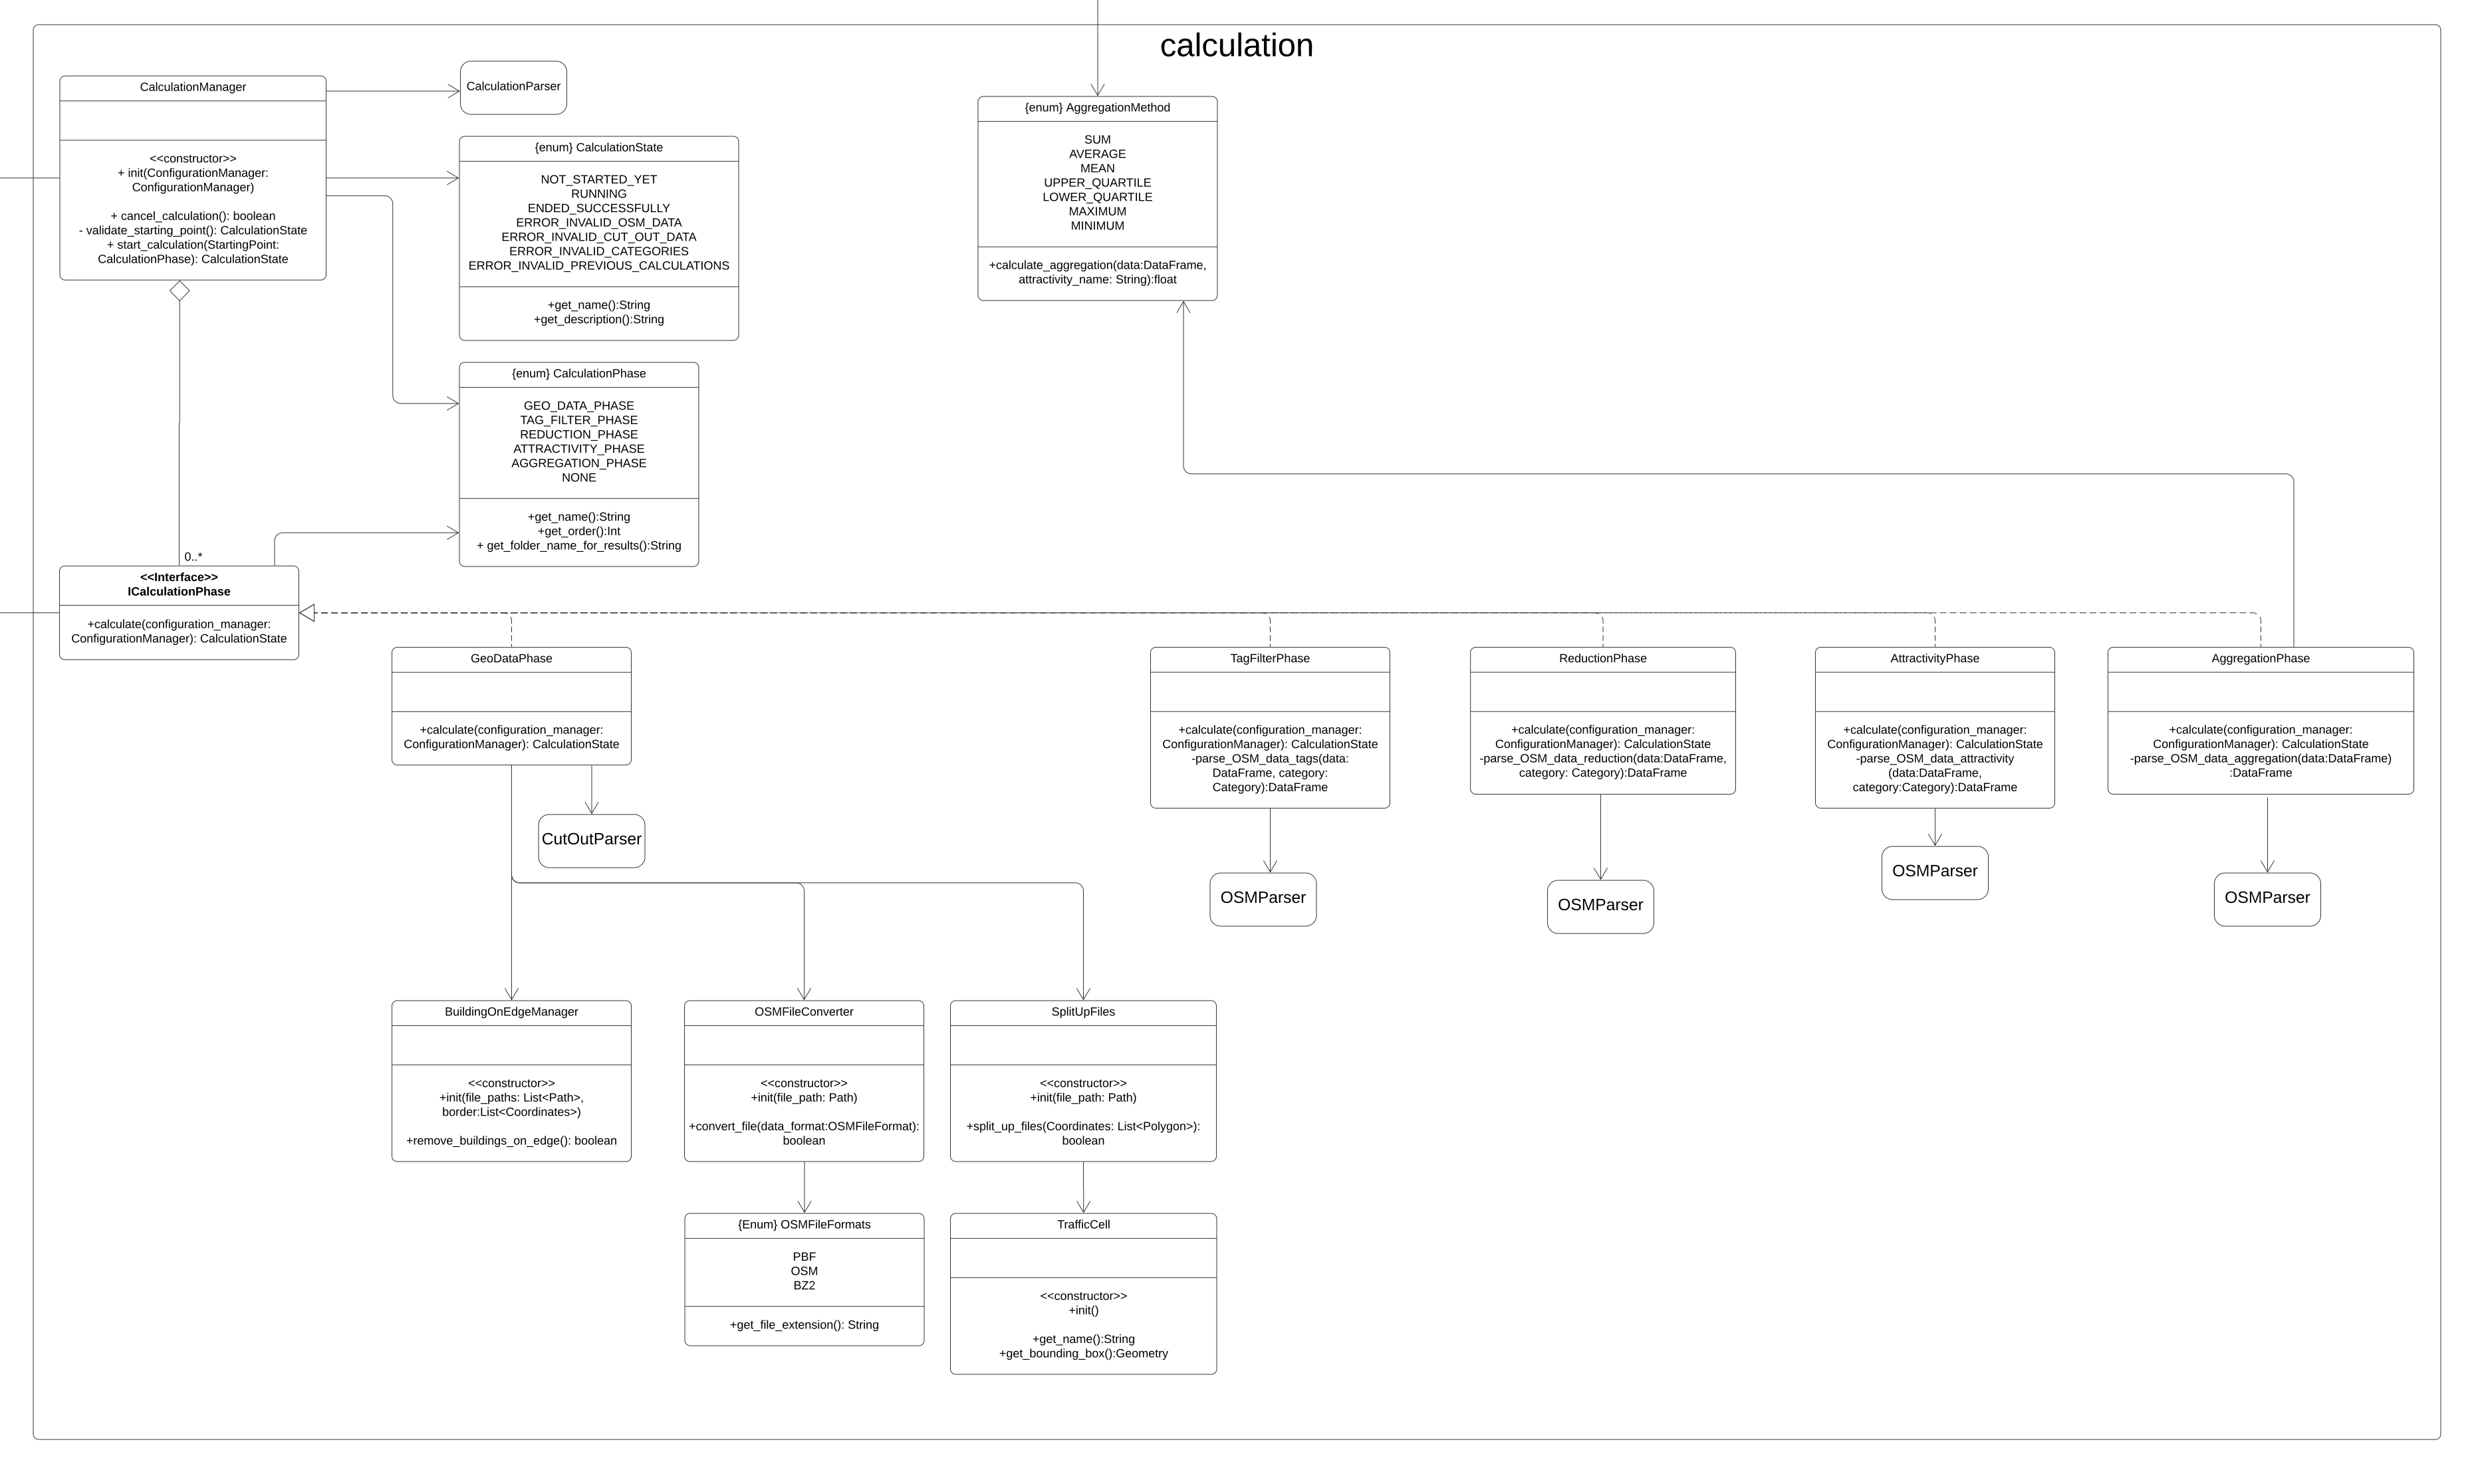
\includegraphics[width=0.8\textwidth]
        {pictures/calculation.png}
  \caption{Package: calculation}
  \label{fig:calculation}
\end{figure}
}


\newpage% for dupelx printing


\chapter{Software Patterns}
\label{\detokenize{index:software-patterns}}
\sphinxstepscope

\section{MVC}
This project uses the Model-View-Controller pattern as described in \ref{sec::mvc}.

\section{Facade}

\subsection{Definition}
The Facade-Pattern hides the complexities of the system providing an abstract class to the client that can access the system. This interface is implemented by using a single class providing the necessary functionality. This helps fighting code redundancy, makes creating new frames easier and therefore reduces debugging efforts.

\subsection{Usage}
This project uses the facade-pattern in the view-package. By implementing a parent providing basic-functionality to its children, code duplications implementing the same functionality can be avoided. Child classes can overwrite the given methods if necessary and implement new features and attributes.
A lot of view-classes implement only small tweaks in a default-functionality-environment while creating new windows. The AggregationFrame for example only has small functionality-tweaks to the SettingsFrame. The different appearance of the frames is implemented separately, but the base-functionality of e.g. pressing a button is implemented only once.



\chapter{Sequence Diagram}
\label{\detokenize{index:sequence-diagrams}}
\sphinxstepscope
The sequence diagram below (figure \ref{fig:sequencediagram}) shows how the application behaves when switching to the category frame and when the user creates a new category. This example shows two important mechanisms of our design:\\
Firstly, it shows how switching states works in the view. The StateManager is informed, when the state needs to be changed. It decides which frames must be shown to the user and forwards the request to the MainWindow. When a frame is activated, it's activate() method is invoked. \\
Secondly, the communication between the view, the control and the model is shown. Frames of the view message requests to the control. The control forwards the message to the model. The request is answered via return values.

\begin{sidewaysfigure}
\centering
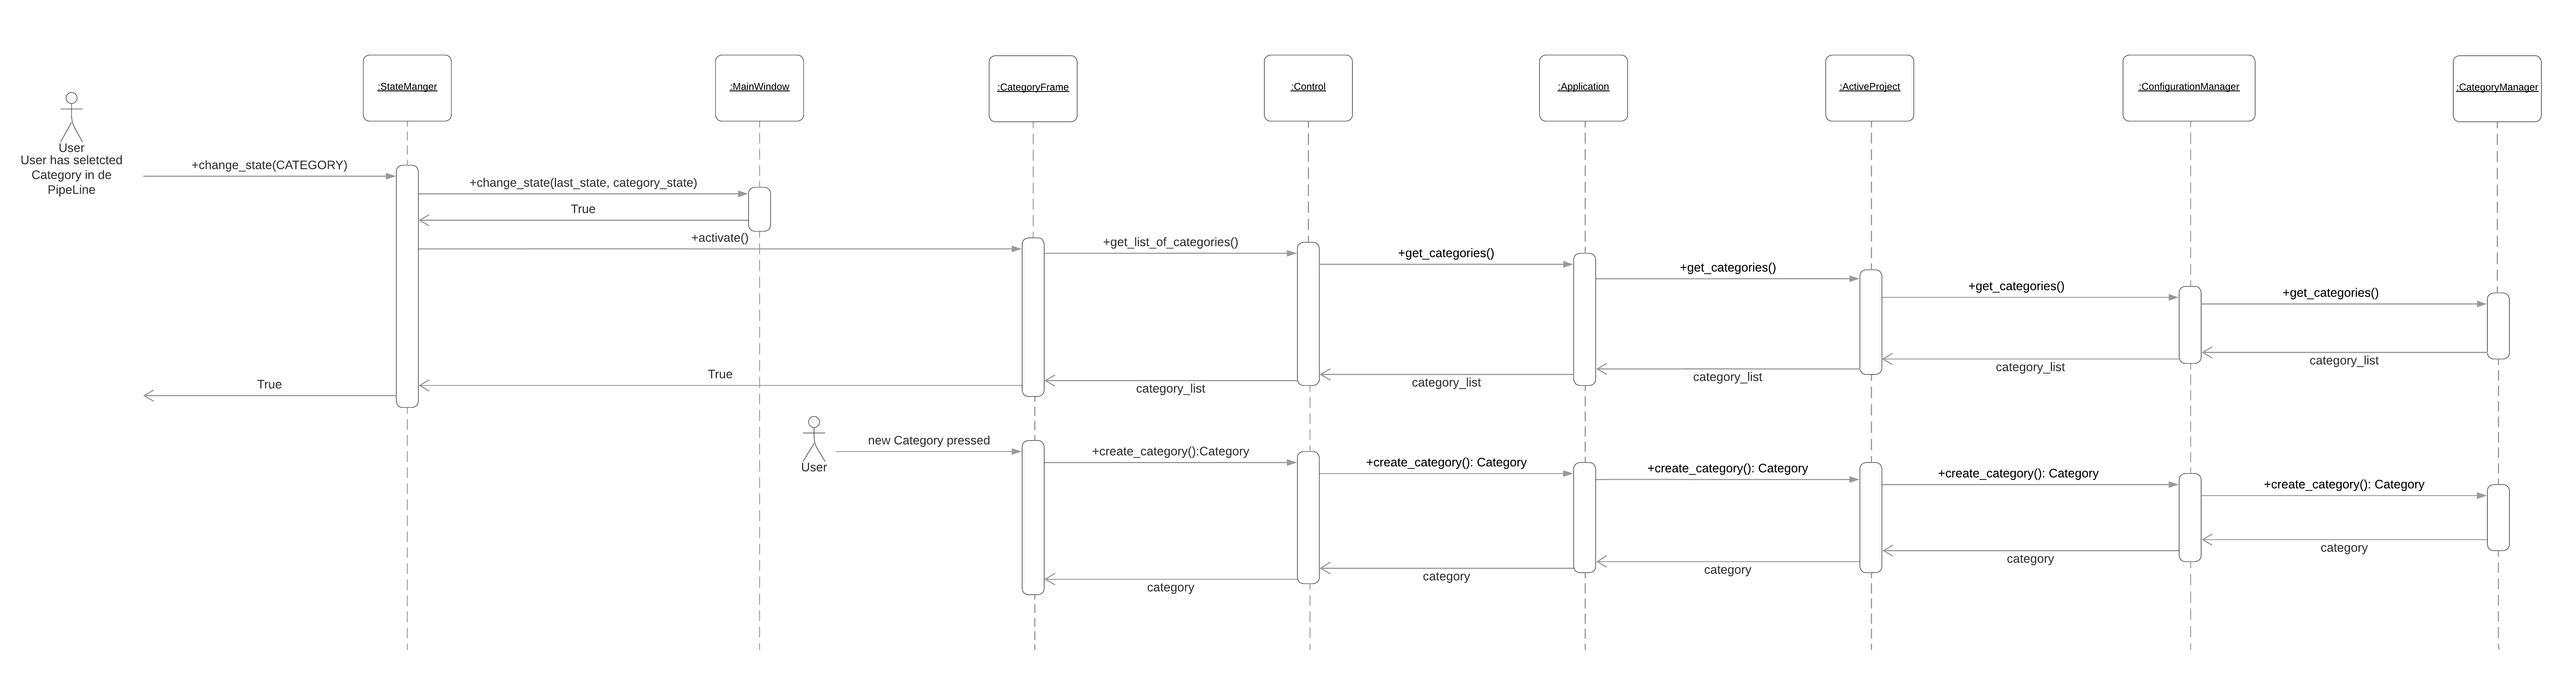
\includegraphics[width=1\textwidth]
        {pictures/sequenzdiagramm.png}
  \caption{sequence diagram}
  \label{fig:sequencediagram}
\end{sidewaysfigure}


\newpage% for dupelx printing


\chapter{Libraries}
\label{\detokenize{index:libaries}}
\sphinxstepscope

\section{Frontend and Dashboard}

\subsection{CustomTkinter}

\paragraph{What is CustomTkinter?}
\href{https://github.com/TomSchimansky/CustomTkinter}{CustomTkinter} is a python GUI-library based on Tkinter, which provides new, modern and fully customizable widgets. They are created and used like normal Tkinter widgets and can also be used in combination with normal Tkinter elements. 

\paragraph{Why use CustomTkinter?}
We decided to use CustomTkinter as a GUI-library, because TKinter is an easy to use library, which is standard in Python ecosystem.
But Tkinter alone looks a bit outdated, CustomTkinter provides Tkinter in a more modern look.

\paragraph{Why not use other libararies?}
CustomTkinter had a couple of alternatives that could have been used but all of them had disadvantages that made them worse in our use case than CustomTkinter. 
  
\textbf{Tkinter}
\begin{itemize}
    \item Same features as CustomTkinter but has a more aged look.
\end{itemize}
  
\textbf{Pyqt5}
\begin{itemize}
    \item Offers more features compared to CustomTkinter, but is more complicated and these additional features are not needed in our project.
    \item PyQT5 is not free for commercial use, it's better to have a more lenient licence.
\end{itemize}
\textbf{Kivy}
\begin{itemize}
    \item Offers more features compared to CustomTkinter, but is more complicated and these additional features are not needed in our project. 
\end{itemize}


\subsection{Seaborn}
\paragraph{What is Seaborn?}
\href{https://seaborn.pydata.org/}{Seaborn} is a Python data visualization library based on matplotlib. It provides a high-level interface for drawing attractive and informative statistical graphics.

\paragraph{Why use Seaborn?}
In our application we use Seaborn to visualize the endresult of the calculation.

\paragraph{Why not use other libararies?}
The only really other alternative to Seaborn is matplotlib which can do the same as Seaborn, but Seaborn is more easily usable then matplotlib, furthermore Seaborn uses matplotlib in the background to create and visualize their results.




\section{Backend}
% Ist es besser hier nach Model, View und Controller zu sortieren?

\subsection{osmium-tool}

\paragraph{What is osmium-tool?}
\href{https://osmcode.org/osmium-tool/}{Osmium}
is a versatile command line tool for working with OpenStreetMap data. It includes many useful functions for manipulating OSM data and often outperforms similar tools.

\paragraph{Why use osmium-tool?}
In our application we will deal with very large OSM-Data files.
The osmium-tool allows us to convert from one OSM-Data file format to another one. 
Furthermore it can be used to split large OSM-Data files into multiple smaller ones, which we will use to split the OSM-Data into the previously defined 
\hyperref[sec:Glossary]{traffic cells}.

\paragraph{Why not use other libararies?}
Osmium-tool doesn't really have competitors in it's space, there aren't any mature python libraries which can cut OSM-data files like osmium-tool.
Though there are libraries/application written in different languages that can do what Osmium-tool does, such as Osmosis or osmfilter.
But they are slower or require additional software such as java.


\subsection{Osmium}

\paragraph{What is Osmium?}
The \href{https://osmcode.org/libosmium/}{Osmium} Library has extensive support for all types of OSM entities: nodes, ways, relations, and changesets. It allows reading from and writing to OSM files in XML, PBF, and several other formats, including change files and full history files. Osmium can store OSM data in memory and on disk in various formats and using various indexes.

\paragraph{Why use Osmium?}
In out application we use Osmium to parse buildings out of the OSM-Data file.

\paragraph{Why not use other libararies?}
Osmium had a couple of alternatives that could have been used but all of them had disadvantages that made them worse in our use case than Osmium. 
  
\textbf{OSMnx}
\begin{itemize}
    \item Is more used for network, such as street networks. 
    \item When trying it out, it was hard to work with.
\end{itemize}


\textbf{Pyrosm}
\begin{itemize}
    \item Pyrosm isn't as active developed as it used to be, no support for newer python version, dependencies use old version.
    \item Pyrosm wasn't compatible with the rest of libaries we use, since it depends on old version of libaries.
\end{itemize}

\subsection{Psutil}
\paragraph{What is Psutil?}
\href{https://pypi.org/project/psutil/}{Psutil}(process and system utilities) is a cross-platform library for retrieving information on running processes and system utilization (CPU, memory, disks, network, sensors) in Python. It is useful mainly for system monitoring, profiling and limiting process resources and management of running processes. 

\paragraph{Why use Psutil?}
In our Project we use Psutil to monitor the RAM usage, this is required for decision like: how much OSM-Data do we load simultaneous in the RAM?

\paragraph{Why not use other libararies?}
Psutil is a small  library, that does what it promises to do, it is not needed to find a "better" library.

\subsection{Sphinx}

\paragraph{What is Sphinx?}
\href{https://www.sphinx-doc.org/en/master/}{Sphinx} is a documentation generator written and used by the Python community, it makes it easy to create intelligent and beautiful documentation.
It can generate web pages, printable PDFs, documents for e-readers (ePub), and more all from the same sources.

\paragraph{Why use Sphinx?}
Sphinx allows us to easily document our code and make this beautiful document.

\paragraph{Why not use other libararies?}
Sphinx is industry standard when it comes to generating documenting from your code.

\subsection{osmnx}

\paragraph{What is osmnx?}
\href{https://osmnx.readthedocs.io/en/stable/}{OSMnx} is a Python package that lets you download geospatial data from OpenStreetMap and model, project, visualize, and analyze real-world street networks and any other geospatial geometries. You can download and model walkable, drivable, or bikeable urban networks with a single line of Python code then easily analyze and visualize them. You can just as easily download and work with other infrastructure types, amenities/points of interest, building footprints, elevation data, street bearings/orientations, and speed/travel time.

\paragraph{Why use osmnx?}
In our project we use use osmnx to download OSM Data to the project (Desirable criterion).

\section{Miscellaneous}
The Previously described libraries have many dependencies, that may also be used such as:
\begin{itemize}
    \item tkinter
    \item geopandas
    \item numpy
    \item shapely
    \item folium
    \item etc.
\end{itemize}


% for duplex printing
\newpage



\chapter{Class Descriptions}
\label{\detokenize{index:class-descriptions}}
\sphinxstepscope


\section{Control Package}

\paragraph{Submodules}
\label{\detokenize{apidoc/src.osm_configurator.control:submodules}}

\subparagraph{src.osm\_configurator.control.aggregation\_controller module}
\label{\detokenize{apidoc/src.osm_configurator.control:module-src.osm_configurator.control.aggregation_controller}}\label{\detokenize{apidoc/src.osm_configurator.control:src-osm-configurator-control-aggregation-controller-module}}\index{module@\spxentry{module}!src.osm\_configurator.control.aggregation\_controller@\spxentry{src.osm\_configurator.control.aggregation\_controller}}\index{src.osm\_configurator.control.aggregation\_controller@\spxentry{src.osm\_configurator.control.aggregation\_controller}!module@\spxentry{module}}\index{AggregationController (class in src.osm\_configurator.control.aggregation\_controller)@\spxentry{AggregationController}\spxextra{class in src.osm\_configurator.control.aggregation\_controller}}

\begin{fulllineitems}
\phantomsection\label{\detokenize{apidoc/src.osm_configurator.control:src.osm_configurator.control.aggregation_controller.AggregationController}}
\pysigstartsignatures
\pysiglinewithargsret{\sphinxbfcode{\sphinxupquote{class\DUrole{w}{  }}}\sphinxbfcode{\sphinxupquote{AggregationController}}}{\emph{\DUrole{n}{model}}}{}
\pysigstopsignatures
\sphinxAtStartPar
Bases: \sphinxhref{https://docs.python.org/3.11/library/functions.html\#object}{\sphinxcode{\sphinxupquote{object}}}

\sphinxAtStartPar
The AggregationController is responsible for consistently forwarding requests to the model, regarding the aggregation\sphinxhyphen{}calculations and the aggregation methods of the currently selected project.
\index{\_\_init\_\_() (AggregationController method)@\spxentry{\_\_init\_\_()}\spxextra{AggregationController method}}

\begin{fulllineitems}
\phantomsection\label{\detokenize{apidoc/src.osm_configurator.control:src.osm_configurator.control.aggregation_controller.AggregationController.__init__}}
\pysigstartsignatures
\pysiglinewithargsret{\sphinxbfcode{\sphinxupquote{\_\_init\_\_}}}{\emph{\DUrole{n}{model}}}{}
\pysigstopsignatures
\sphinxAtStartPar
Creates a new instance of the AggregationController, with an association to the model.
\begin{quote}\begin{description}
\sphinxlineitem{Parameters}
\sphinxAtStartPar
\sphinxstyleliteralstrong{\sphinxupquote{model}} ({\hyperref[\detokenize{apidoc/src.osm_configurator.model.application:src.osm_configurator.model.application.application_interface.IApplication}]{\sphinxcrossref{\sphinxstyleliteralemphasis{\sphinxupquote{application\_interface.IApplication}}}}}) \textendash{} The interface which is used to communicate with the model.

\end{description}\end{quote}

\end{fulllineitems}

\index{get\_aggregation\_methods() (AggregationController method)@\spxentry{get\_aggregation\_methods()}\spxextra{AggregationController method}}

\begin{fulllineitems}
\phantomsection\label{\detokenize{apidoc/src.osm_configurator.control:src.osm_configurator.control.aggregation_controller.AggregationController.get_aggregation_methods}}
\pysigstartsignatures
\pysiglinewithargsret{\sphinxbfcode{\sphinxupquote{get\_aggregation\_methods}}}{}{}
\pysigstopsignatures
\sphinxAtStartPar
Returns a list of all aggregation methods that are available.
This function returns all available aggregation methods, not just the ones that are active in the current project.
\begin{quote}\begin{description}
\sphinxlineitem{Returns}
\sphinxAtStartPar
The list of the available aggregation methods

\sphinxlineitem{Return type}
\sphinxAtStartPar
\sphinxhref{https://docs.python.org/3.11/library/stdtypes.html\#list}{list}{[}{\hyperref[\detokenize{apidoc/src.osm_configurator.model.project.calculation:src.osm_configurator.model.project.calculation.aggregation_method_enum.AggregationMethod}]{\sphinxcrossref{aggregation\_method\_enum.AggregationMethod}}}{]}

\end{description}\end{quote}

\end{fulllineitems}

\index{is\_aggregation\_method\_active() (AggregationController method)@\spxentry{is\_aggregation\_method\_active()}\spxextra{AggregationController method}}

\begin{fulllineitems}
\phantomsection\label{\detokenize{apidoc/src.osm_configurator.control:src.osm_configurator.control.aggregation_controller.AggregationController.is_aggregation_method_active}}
\pysigstartsignatures
\pysiglinewithargsret{\sphinxbfcode{\sphinxupquote{is\_aggregation\_method\_active}}}{\emph{\DUrole{n}{method}}}{}
\pysigstopsignatures
\sphinxAtStartPar
Checks, whether an aggregation method is active in the currently selected project.
\begin{quote}\begin{description}
\sphinxlineitem{Parameters}
\sphinxAtStartPar
\sphinxstyleliteralstrong{\sphinxupquote{method}} ({\hyperref[\detokenize{apidoc/src.osm_configurator.model.project.calculation:src.osm_configurator.model.project.calculation.aggregation_method_enum.AggregationMethod}]{\sphinxcrossref{\sphinxstyleliteralemphasis{\sphinxupquote{aggregation\_method\_enum.AggregationMethod}}}}}) \textendash{} The aggregation method that is checked for.

\sphinxlineitem{Returns}
\sphinxAtStartPar
True, if there is currently a project selected and the given aggregation method is active in it; False otherwise.

\sphinxlineitem{Return type}
\sphinxAtStartPar
\sphinxhref{https://docs.python.org/3.11/library/functions.html\#bool}{bool}

\end{description}\end{quote}

\end{fulllineitems}

\index{set\_aggregation\_method\_active() (AggregationController method)@\spxentry{set\_aggregation\_method\_active()}\spxextra{AggregationController method}}

\begin{fulllineitems}
\phantomsection\label{\detokenize{apidoc/src.osm_configurator.control:src.osm_configurator.control.aggregation_controller.AggregationController.set_aggregation_method_active}}
\pysigstartsignatures
\pysiglinewithargsret{\sphinxbfcode{\sphinxupquote{set\_aggregation\_method\_active}}}{\emph{\DUrole{n}{method}}, \emph{\DUrole{n}{active}}}{}
\pysigstopsignatures
\sphinxAtStartPar
Activates or deactivates an aggregation method (of the currently selected project).
Activates the given method, if active=True and deactivates it otherwise.
\begin{quote}\begin{description}
\sphinxlineitem{Parameters}\begin{itemize}
\item {} 
\sphinxAtStartPar
\sphinxstyleliteralstrong{\sphinxupquote{method}} ({\hyperref[\detokenize{apidoc/src.osm_configurator.model.project.calculation:src.osm_configurator.model.project.calculation.aggregation_method_enum.AggregationMethod}]{\sphinxcrossref{\sphinxstyleliteralemphasis{\sphinxupquote{aggregation\_method\_enum.AggregationMethod}}}}}) \textendash{} The aggregation method we want to deactivate/activate

\item {} 
\sphinxAtStartPar
\sphinxstyleliteralstrong{\sphinxupquote{active}} (\sphinxhref{https://docs.python.org/3.11/library/functions.html\#bool}{\sphinxstyleliteralemphasis{\sphinxupquote{bool}}}) \textendash{} True, if we want to activate the given method; False, if we want to deactivate it.

\end{itemize}

\sphinxlineitem{Returns}
\sphinxAtStartPar
True, if a project is currently selected and the aggregation method was (de\sphinxhyphen{})activated successfully; False, otherwise.

\sphinxlineitem{Return type}
\sphinxAtStartPar
\sphinxhref{https://docs.python.org/3.11/library/functions.html\#bool}{bool}

\end{description}\end{quote}

\end{fulllineitems}


\end{fulllineitems}



\subparagraph{src.osm\_configurator.control.application\_controller module}
\label{\detokenize{apidoc/src.osm_configurator.control:module-src.osm_configurator.control.application_controller}}\label{\detokenize{apidoc/src.osm_configurator.control:src-osm-configurator-control-application-controller-module}}\index{module@\spxentry{module}!src.osm\_configurator.control.application\_controller@\spxentry{src.osm\_configurator.control.application\_controller}}\index{src.osm\_configurator.control.application\_controller@\spxentry{src.osm\_configurator.control.application\_controller}!module@\spxentry{module}}\index{ApplicationController (class in src.osm\_configurator.control.application\_controller)@\spxentry{ApplicationController}\spxextra{class in src.osm\_configurator.control.application\_controller}}

\begin{fulllineitems}
\phantomsection\label{\detokenize{apidoc/src.osm_configurator.control:src.osm_configurator.control.application_controller.ApplicationController}}
\pysigstartsignatures
\pysigline{\sphinxbfcode{\sphinxupquote{class\DUrole{w}{  }}}\sphinxbfcode{\sphinxupquote{ApplicationController}}}
\pysigstopsignatures
\sphinxAtStartPar
Bases: \sphinxhref{https://docs.python.org/3.11/library/functions.html\#object}{\sphinxcode{\sphinxupquote{object}}}

\sphinxAtStartPar
The application controller is responsible for creating the model, the view and the control. It is the start of the
application and boots everything up.
\index{main() (ApplicationController method)@\spxentry{main()}\spxextra{ApplicationController method}}

\begin{fulllineitems}
\phantomsection\label{\detokenize{apidoc/src.osm_configurator.control:src.osm_configurator.control.application_controller.ApplicationController.main}}
\pysigstartsignatures
\pysiglinewithargsret{\sphinxbfcode{\sphinxupquote{main}}}{}{}
\pysigstopsignatures
\sphinxAtStartPar
Starts the application.
This class method’s only job is, to give control to an instance of the ApplicationController.

\end{fulllineitems}

\index{\_\_init\_\_() (ApplicationController method)@\spxentry{\_\_init\_\_()}\spxextra{ApplicationController method}}

\begin{fulllineitems}
\phantomsection\label{\detokenize{apidoc/src.osm_configurator.control:src.osm_configurator.control.application_controller.ApplicationController.__init__}}
\pysigstartsignatures
\pysiglinewithargsret{\sphinxbfcode{\sphinxupquote{\_\_init\_\_}}}{}{}
\pysigstopsignatures
\sphinxAtStartPar
Creates a new Application. It creates the view, the model and the control. It is responsible for starting
everything up and to switch to the normal workflow of the application.

\end{fulllineitems}


\end{fulllineitems}



\subparagraph{src.osm\_configurator.control.calculation\_controller module}
\label{\detokenize{apidoc/src.osm_configurator.control:module-src.osm_configurator.control.calculation_controller}}\label{\detokenize{apidoc/src.osm_configurator.control:src-osm-configurator-control-calculation-controller-module}}\index{module@\spxentry{module}!src.osm\_configurator.control.calculation\_controller@\spxentry{src.osm\_configurator.control.calculation\_controller}}\index{src.osm\_configurator.control.calculation\_controller@\spxentry{src.osm\_configurator.control.calculation\_controller}!module@\spxentry{module}}\index{CalculationController (class in src.osm\_configurator.control.calculation\_controller)@\spxentry{CalculationController}\spxextra{class in src.osm\_configurator.control.calculation\_controller}}

\begin{fulllineitems}
\phantomsection\label{\detokenize{apidoc/src.osm_configurator.control:src.osm_configurator.control.calculation_controller.CalculationController}}
\pysigstartsignatures
\pysiglinewithargsret{\sphinxbfcode{\sphinxupquote{class\DUrole{w}{  }}}\sphinxbfcode{\sphinxupquote{CalculationController}}}{\emph{\DUrole{n}{model}}}{}
\pysigstopsignatures
\sphinxAtStartPar
Bases: \sphinxhref{https://docs.python.org/3.11/library/functions.html\#object}{\sphinxcode{\sphinxupquote{object}}}

\sphinxAtStartPar
The CalculationController is responsible for forwarding requests to the model, regarding calculations.
It may be used to gather information and to control the calculation\sphinxhyphen{}process of the currently selected project.
\index{\_\_init\_\_() (CalculationController method)@\spxentry{\_\_init\_\_()}\spxextra{CalculationController method}}

\begin{fulllineitems}
\phantomsection\label{\detokenize{apidoc/src.osm_configurator.control:src.osm_configurator.control.calculation_controller.CalculationController.__init__}}
\pysigstartsignatures
\pysiglinewithargsret{\sphinxbfcode{\sphinxupquote{\_\_init\_\_}}}{\emph{\DUrole{n}{model}}}{}
\pysigstopsignatures
\sphinxAtStartPar
Creates a new instance of the CalculationController, with an association to the model.
\begin{quote}\begin{description}
\sphinxlineitem{Parameters}
\sphinxAtStartPar
\sphinxstyleliteralstrong{\sphinxupquote{model}} ({\hyperref[\detokenize{apidoc/src.osm_configurator.model.application:src.osm_configurator.model.application.application_interface.IApplication}]{\sphinxcrossref{\sphinxstyleliteralemphasis{\sphinxupquote{application\_interface.IApplication}}}}}) \textendash{} The interface which is used to communicate with the model.

\end{description}\end{quote}

\end{fulllineitems}

\index{start\_calculations() (CalculationController method)@\spxentry{start\_calculations()}\spxextra{CalculationController method}}

\begin{fulllineitems}
\phantomsection\label{\detokenize{apidoc/src.osm_configurator.control:src.osm_configurator.control.calculation_controller.CalculationController.start_calculations}}
\pysigstartsignatures
\pysiglinewithargsret{\sphinxbfcode{\sphinxupquote{start\_calculations}}}{\emph{\DUrole{n}{starting\_phase}}}{}
\pysigstopsignatures
\sphinxAtStartPar
Starts the calculations in the given calculation phase in the currently selected project.
The calculation process is split in different calculation phases. This function starts the calculation in a given phase.
\begin{quote}\begin{description}
\sphinxlineitem{Parameters}
\sphinxAtStartPar
\sphinxstyleliteralstrong{\sphinxupquote{starting\_phase}} ({\hyperref[\detokenize{apidoc/src.osm_configurator.model.project.calculation:src.osm_configurator.model.project.calculation.calculation_phase_enum.CalculationPhase}]{\sphinxcrossref{\sphinxstyleliteralemphasis{\sphinxupquote{calculation\_phase\_enum.CalculationPhase}}}}}) \textendash{} The phase, in which the calculation should start

\sphinxlineitem{Returns}
\sphinxAtStartPar
The status of the calculation: RUNNING, if the calculation was started successfully. For details on the meaning of this return value, see CalculationState

\sphinxlineitem{Return type}
\sphinxAtStartPar
{\hyperref[\detokenize{apidoc/src.osm_configurator.model.project.calculation:src.osm_configurator.model.project.calculation.calculation_state_enum.CalculationState}]{\sphinxcrossref{calculation\_state\_enum.CalculationState}}}

\end{description}\end{quote}

\end{fulllineitems}

\index{get\_calculation\_state() (CalculationController method)@\spxentry{get\_calculation\_state()}\spxextra{CalculationController method}}

\begin{fulllineitems}
\phantomsection\label{\detokenize{apidoc/src.osm_configurator.control:src.osm_configurator.control.calculation_controller.CalculationController.get_calculation_state}}
\pysigstartsignatures
\pysiglinewithargsret{\sphinxbfcode{\sphinxupquote{get\_calculation\_state}}}{}{}
\pysigstopsignatures
\sphinxAtStartPar
Gives the current calculation state of the selected project.
\begin{quote}\begin{description}
\sphinxlineitem{Returns}
\sphinxAtStartPar
Returns the current state of the calculation. For details see documentation of CalculationState.

\sphinxlineitem{Return type}
\sphinxAtStartPar
{\hyperref[\detokenize{apidoc/src.osm_configurator.model.project.calculation:src.osm_configurator.model.project.calculation.calculation_state_enum.CalculationState}]{\sphinxcrossref{calculation\_state\_enum.CalculationState}}}

\end{description}\end{quote}

\end{fulllineitems}

\index{get\_current\_calculation\_phase() (CalculationController method)@\spxentry{get\_current\_calculation\_phase()}\spxextra{CalculationController method}}

\begin{fulllineitems}
\phantomsection\label{\detokenize{apidoc/src.osm_configurator.control:src.osm_configurator.control.calculation_controller.CalculationController.get_current_calculation_phase}}
\pysigstartsignatures
\pysiglinewithargsret{\sphinxbfcode{\sphinxupquote{get\_current\_calculation\_phase}}}{}{}
\pysigstopsignatures
\sphinxAtStartPar
Returns the calculation phase of the currently selected project.
\begin{quote}\begin{description}
\sphinxlineitem{Returns}
\sphinxAtStartPar
The phase, that is currently running. NONE, if no phase is currently running.

\sphinxlineitem{Return type}
\sphinxAtStartPar
{\hyperref[\detokenize{apidoc/src.osm_configurator.model.project.calculation:src.osm_configurator.model.project.calculation.calculation_phase_enum.CalculationPhase}]{\sphinxcrossref{calculation\_phase\_enum.CalculationPhase}}}

\end{description}\end{quote}

\end{fulllineitems}

\index{get\_current\_calculation\_process() (CalculationController method)@\spxentry{get\_current\_calculation\_process()}\spxextra{CalculationController method}}

\begin{fulllineitems}
\phantomsection\label{\detokenize{apidoc/src.osm_configurator.control:src.osm_configurator.control.calculation_controller.CalculationController.get_current_calculation_process}}
\pysigstartsignatures
\pysiglinewithargsret{\sphinxbfcode{\sphinxupquote{get\_current\_calculation\_process}}}{}{}
\pysigstopsignatures
\sphinxAtStartPar
Returns an approximation of the progress of the calculations in the currently selected project.
The progress is given as a number between 0 and 1, where 0 indicates that the calculation has not started yet and 1 indicates, that the calculations are done.
\begin{quote}\begin{description}
\sphinxlineitem{Returns}
\sphinxAtStartPar
The value of the approximation.

\sphinxlineitem{Return type}
\sphinxAtStartPar
\sphinxhref{https://docs.python.org/3.11/library/functions.html\#float}{float}

\end{description}\end{quote}

\end{fulllineitems}

\index{cancel\_calculations() (CalculationController method)@\spxentry{cancel\_calculations()}\spxextra{CalculationController method}}

\begin{fulllineitems}
\phantomsection\label{\detokenize{apidoc/src.osm_configurator.control:src.osm_configurator.control.calculation_controller.CalculationController.cancel_calculations}}
\pysigstartsignatures
\pysiglinewithargsret{\sphinxbfcode{\sphinxupquote{cancel\_calculations}}}{}{}
\pysigstopsignatures
\sphinxAtStartPar
Cancels the calculations of the currently selected project.
The calculation phase that is currently running will be stopped.
\begin{quote}\begin{description}
\sphinxlineitem{Returns}
\sphinxAtStartPar
True, if the calculation was canceled successfully; False, otherwise.

\sphinxlineitem{Return type}
\sphinxAtStartPar
\sphinxhref{https://docs.python.org/3.11/library/functions.html\#bool}{bool}

\end{description}\end{quote}

\end{fulllineitems}


\end{fulllineitems}



\subparagraph{src.osm\_configurator.control.category\_controller module}
\label{\detokenize{apidoc/src.osm_configurator.control:module-src.osm_configurator.control.category_controller}}\label{\detokenize{apidoc/src.osm_configurator.control:src-osm-configurator-control-category-controller-module}}\index{module@\spxentry{module}!src.osm\_configurator.control.category\_controller@\spxentry{src.osm\_configurator.control.category\_controller}}\index{src.osm\_configurator.control.category\_controller@\spxentry{src.osm\_configurator.control.category\_controller}!module@\spxentry{module}}\index{CategoryController (class in src.osm\_configurator.control.category\_controller)@\spxentry{CategoryController}\spxextra{class in src.osm\_configurator.control.category\_controller}}

\begin{fulllineitems}
\phantomsection\label{\detokenize{apidoc/src.osm_configurator.control:src.osm_configurator.control.category_controller.CategoryController}}
\pysigstartsignatures
\pysiglinewithargsret{\sphinxbfcode{\sphinxupquote{class\DUrole{w}{  }}}\sphinxbfcode{\sphinxupquote{CategoryController}}}{\emph{\DUrole{n}{model}}}{}
\pysigstopsignatures
\sphinxAtStartPar
Bases: \sphinxhref{https://docs.python.org/3.11/library/functions.html\#object}{\sphinxcode{\sphinxupquote{object}}}

\sphinxAtStartPar
The CategoryController is responsible for consistently forwarding requests to the model,
regarding changes to the categories of the current project.
\index{\_\_init\_\_() (CategoryController method)@\spxentry{\_\_init\_\_()}\spxextra{CategoryController method}}

\begin{fulllineitems}
\phantomsection\label{\detokenize{apidoc/src.osm_configurator.control:src.osm_configurator.control.category_controller.CategoryController.__init__}}
\pysigstartsignatures
\pysiglinewithargsret{\sphinxbfcode{\sphinxupquote{\_\_init\_\_}}}{\emph{\DUrole{n}{model}}}{}
\pysigstopsignatures
\sphinxAtStartPar
Creates a new instance of the CategoryController, with an association to the model.
\begin{quote}\begin{description}
\sphinxlineitem{Parameters}
\sphinxAtStartPar
\sphinxstyleliteralstrong{\sphinxupquote{model}} ({\hyperref[\detokenize{apidoc/src.osm_configurator.model.application:src.osm_configurator.model.application.application_interface.IApplication}]{\sphinxcrossref{\sphinxstyleliteralemphasis{\sphinxupquote{application\_interface.IApplication}}}}}) \textendash{} The interface which is used to communicate with the model.

\end{description}\end{quote}

\end{fulllineitems}

\index{check\_conflicts\_in\_category\_configuration() (CategoryController method)@\spxentry{check\_conflicts\_in\_category\_configuration()}\spxextra{CategoryController method}}

\begin{fulllineitems}
\phantomsection\label{\detokenize{apidoc/src.osm_configurator.control:src.osm_configurator.control.category_controller.CategoryController.check_conflicts_in_category_configuration}}
\pysigstartsignatures
\pysiglinewithargsret{\sphinxbfcode{\sphinxupquote{check\_conflicts\_in\_category\_configuration}}}{\emph{\DUrole{n}{path}}}{}
\pysigstopsignatures
\sphinxAtStartPar
Checks for a given file, if it is a valid category\sphinxhyphen{}file and checks, whether there are naming conflicts with the categories of the currently selected project.
\begin{quote}\begin{description}
\sphinxlineitem{Parameters}
\sphinxAtStartPar
\sphinxstyleliteralstrong{\sphinxupquote{path}} (\sphinxhref{https://docs.python.org/3.11/library/pathlib.html\#pathlib.Path}{\sphinxstyleliteralemphasis{\sphinxupquote{pathlib.Path}}}) \textendash{} The path to the category\sphinxhyphen{}file

\sphinxlineitem{Returns}
\sphinxAtStartPar
True, if there is currently a project selected and there are no naming conflicts; False, otherwise.

\sphinxlineitem{Return type}
\sphinxAtStartPar
\sphinxhref{https://docs.python.org/3.11/library/functions.html\#bool}{bool}

\end{description}\end{quote}

\end{fulllineitems}

\index{import\_category\_configuration() (CategoryController method)@\spxentry{import\_category\_configuration()}\spxextra{CategoryController method}}

\begin{fulllineitems}
\phantomsection\label{\detokenize{apidoc/src.osm_configurator.control:src.osm_configurator.control.category_controller.CategoryController.import_category_configuration}}
\pysigstartsignatures
\pysiglinewithargsret{\sphinxbfcode{\sphinxupquote{import\_category\_configuration}}}{\emph{\DUrole{n}{path}}}{}
\pysigstopsignatures
\sphinxAtStartPar
Imports the given categories into the currently selected project.
Adds the given categories to the category list of the project.
\begin{quote}\begin{description}
\sphinxlineitem{Parameters}
\sphinxAtStartPar
\sphinxstyleliteralstrong{\sphinxupquote{path}} (\sphinxhref{https://docs.python.org/3.11/library/pathlib.html\#pathlib.Path}{\sphinxstyleliteralemphasis{\sphinxupquote{pathlib.Path}}}) \textendash{} The path to the category file

\sphinxlineitem{Returns}
\sphinxAtStartPar
True, if the categories where added successfully; False, if there is no project loaded, the category file is corrupted or the category file does not exist.

\sphinxlineitem{Return type}
\sphinxAtStartPar
\sphinxhref{https://docs.python.org/3.11/library/functions.html\#bool}{bool}

\end{description}\end{quote}

\end{fulllineitems}

\index{get\_list\_of\_categories() (CategoryController method)@\spxentry{get\_list\_of\_categories()}\spxextra{CategoryController method}}

\begin{fulllineitems}
\phantomsection\label{\detokenize{apidoc/src.osm_configurator.control:src.osm_configurator.control.category_controller.CategoryController.get_list_of_categories}}
\pysigstartsignatures
\pysiglinewithargsret{\sphinxbfcode{\sphinxupquote{get\_list\_of\_categories}}}{}{}
\pysigstopsignatures
\sphinxAtStartPar
Returns the list of all categories, that are currently in the currently selected project.
\begin{quote}\begin{description}
\sphinxlineitem{Returns}
\sphinxAtStartPar
A list of the categories of the project in no particular order.

\sphinxlineitem{Return type}
\sphinxAtStartPar
\sphinxhref{https://docs.python.org/3.11/library/stdtypes.html\#list}{list}{[}{\hyperref[\detokenize{apidoc/src.osm_configurator.model.project.configuration:src.osm_configurator.model.project.configuration.category.Category}]{\sphinxcrossref{category.Category}}}{]}

\end{description}\end{quote}

\end{fulllineitems}

\index{create\_category() (CategoryController method)@\spxentry{create\_category()}\spxextra{CategoryController method}}

\begin{fulllineitems}
\phantomsection\label{\detokenize{apidoc/src.osm_configurator.control:src.osm_configurator.control.category_controller.CategoryController.create_category}}
\pysigstartsignatures
\pysiglinewithargsret{\sphinxbfcode{\sphinxupquote{create\_category}}}{}{}
\pysigstopsignatures
\sphinxAtStartPar
Creates a new category in the currently selected project.
A new category is added to the list of categories of the project. The category has empty properties, except for an arbitrary name.
If the creation fails, none will be returned and there won’t be a category added.
\begin{quote}\begin{description}
\sphinxlineitem{Returns}
\sphinxAtStartPar
The newly created category, none if there was an error

\sphinxlineitem{Return type}
\sphinxAtStartPar
{\hyperref[\detokenize{apidoc/src.osm_configurator.model.project.configuration:src.osm_configurator.model.project.configuration.category.Category}]{\sphinxcrossref{category.Category}}}

\end{description}\end{quote}

\end{fulllineitems}

\index{delete\_category() (CategoryController method)@\spxentry{delete\_category()}\spxextra{CategoryController method}}

\begin{fulllineitems}
\phantomsection\label{\detokenize{apidoc/src.osm_configurator.control:src.osm_configurator.control.category_controller.CategoryController.delete_category}}
\pysigstartsignatures
\pysiglinewithargsret{\sphinxbfcode{\sphinxupquote{delete\_category}}}{\emph{\DUrole{n}{category}}}{}
\pysigstopsignatures
\sphinxAtStartPar
Deletes the given category.
Removes the given category from the list of categories of the currently selected project
\begin{quote}\begin{description}
\sphinxlineitem{Parameters}
\sphinxAtStartPar
\sphinxstyleliteralstrong{\sphinxupquote{category}} ({\hyperref[\detokenize{apidoc/src.osm_configurator.model.project.configuration:src.osm_configurator.model.project.configuration.category.Category}]{\sphinxcrossref{\sphinxstyleliteralemphasis{\sphinxupquote{category.Category}}}}}) \textendash{} The category, to be deleted

\sphinxlineitem{Returns}
\sphinxAtStartPar
True, if the category was deleted successfully; False, otherwise

\sphinxlineitem{Return type}
\sphinxAtStartPar
\sphinxhref{https://docs.python.org/3.11/library/functions.html\#bool}{bool}

\end{description}\end{quote}

\end{fulllineitems}

\index{get\_list\_of\_key\_recommendations() (CategoryController method)@\spxentry{get\_list\_of\_key\_recommendations()}\spxextra{CategoryController method}}

\begin{fulllineitems}
\phantomsection\label{\detokenize{apidoc/src.osm_configurator.control:src.osm_configurator.control.category_controller.CategoryController.get_list_of_key_recommendations}}
\pysigstartsignatures
\pysiglinewithargsret{\sphinxbfcode{\sphinxupquote{get\_list\_of\_key\_recommendations}}}{\emph{\DUrole{n}{current\_input}}}{}
\pysigstopsignatures
\sphinxAtStartPar
Returns a list of recommended keys, based on the input that is already entered by the user.
\begin{quote}\begin{description}
\sphinxlineitem{Parameters}
\sphinxAtStartPar
\sphinxstyleliteralstrong{\sphinxupquote{current\_input}} (\sphinxhref{https://docs.python.org/3.11/library/stdtypes.html\#str}{\sphinxstyleliteralemphasis{\sphinxupquote{str}}}) \textendash{} The input, that is currently written by the user.

\sphinxlineitem{Returns}
\sphinxAtStartPar
A list of key recommendations, based on the current\_input.

\sphinxlineitem{Return type}
\sphinxAtStartPar
\sphinxhref{https://docs.python.org/3.11/library/stdtypes.html\#list}{list}{[}\sphinxhref{https://docs.python.org/3.11/library/stdtypes.html\#str}{str}{]}

\end{description}\end{quote}

\end{fulllineitems}

\index{get\_attractivities\_of\_category() (CategoryController method)@\spxentry{get\_attractivities\_of\_category()}\spxextra{CategoryController method}}

\begin{fulllineitems}
\phantomsection\label{\detokenize{apidoc/src.osm_configurator.control:src.osm_configurator.control.category_controller.CategoryController.get_attractivities_of_category}}
\pysigstartsignatures
\pysiglinewithargsret{\sphinxbfcode{\sphinxupquote{get\_attractivities\_of\_category}}}{\emph{\DUrole{n}{category}}}{}
\pysigstopsignatures
\sphinxAtStartPar
Returns the attractivity attributes that are defined for the given category.
\begin{quote}\begin{description}
\sphinxlineitem{Parameters}
\sphinxAtStartPar
\sphinxstyleliteralstrong{\sphinxupquote{category}} ({\hyperref[\detokenize{apidoc/src.osm_configurator.model.project.configuration:src.osm_configurator.model.project.configuration.category.Category}]{\sphinxcrossref{\sphinxstyleliteralemphasis{\sphinxupquote{category.Category}}}}}) \textendash{} The category, whose attractivities are of interest.

\sphinxlineitem{Returns}
\sphinxAtStartPar
The list of attractivity attributes of the given category

\sphinxlineitem{Return type}
\sphinxAtStartPar
\sphinxhref{https://docs.python.org/3.11/library/stdtypes.html\#list}{list}{[}{\hyperref[\detokenize{apidoc/src.osm_configurator.model.project.configuration:src.osm_configurator.model.project.configuration.attractivity_attribute.AttractivityAttribute}]{\sphinxcrossref{attractivity\_attribute.AttractivityAttribute}}}{]}

\end{description}\end{quote}

\end{fulllineitems}


\end{fulllineitems}



\subparagraph{src.osm\_configurator.control.control module}
\label{\detokenize{apidoc/src.osm_configurator.control:module-src.osm_configurator.control.control}}\label{\detokenize{apidoc/src.osm_configurator.control:src-osm-configurator-control-control-module}}\index{module@\spxentry{module}!src.osm\_configurator.control.control@\spxentry{src.osm\_configurator.control.control}}\index{src.osm\_configurator.control.control@\spxentry{src.osm\_configurator.control.control}!module@\spxentry{module}}\index{Control (class in src.osm\_configurator.control.control)@\spxentry{Control}\spxextra{class in src.osm\_configurator.control.control}}

\begin{fulllineitems}
\phantomsection\label{\detokenize{apidoc/src.osm_configurator.control:src.osm_configurator.control.control.Control}}
\pysigstartsignatures
\pysigline{\sphinxbfcode{\sphinxupquote{class\DUrole{w}{  }}}\sphinxbfcode{\sphinxupquote{Control}}}
\pysigstopsignatures
\sphinxAtStartPar
Bases: {\hyperref[\detokenize{apidoc/src.osm_configurator.control:src.osm_configurator.control.control_interface.IControl}]{\sphinxcrossref{\sphinxcode{\sphinxupquote{IControl}}}}}

\sphinxAtStartPar
This class provides a consistent interface for access to the control\sphinxhyphen{}package. It is a facade, to make access easy.
The control manages the access to the module. That’s why this interface should give access to all the features provided by the model.

\sphinxAtStartPar
This implementation of the interface IControl forwards all requests to other classes of this package.
For details see the documentation of the corresponding functions.
\index{\_\_init\_\_() (Control method)@\spxentry{\_\_init\_\_()}\spxextra{Control method}}

\begin{fulllineitems}
\phantomsection\label{\detokenize{apidoc/src.osm_configurator.control:src.osm_configurator.control.control.Control.__init__}}
\pysigstartsignatures
\pysiglinewithargsret{\sphinxbfcode{\sphinxupquote{\_\_init\_\_}}}{}{}
\pysigstopsignatures
\sphinxAtStartPar
Creates a new instance of Control, with a association to the model.
\begin{quote}\begin{description}
\sphinxlineitem{Parameters}
\sphinxAtStartPar
\sphinxstyleliteralstrong{\sphinxupquote{model}} ({\hyperref[\detokenize{apidoc/src.osm_configurator.model.application:src.osm_configurator.model.application.application_interface.IApplication}]{\sphinxcrossref{\sphinxstyleliteralemphasis{\sphinxupquote{application\_interface.IApplication}}}}}) \textendash{} The interface which is used to communicate with the model.

\end{description}\end{quote}

\end{fulllineitems}

\index{get\_list\_of\_passive\_projects() (Control method)@\spxentry{get\_list\_of\_passive\_projects()}\spxextra{Control method}}

\begin{fulllineitems}
\phantomsection\label{\detokenize{apidoc/src.osm_configurator.control:src.osm_configurator.control.control.Control.get_list_of_passive_projects}}
\pysigstartsignatures
\pysiglinewithargsret{\sphinxbfcode{\sphinxupquote{get\_list\_of\_passive\_projects}}}{}{}
\pysigstopsignatures
\sphinxAtStartPar
Returns the list of (passive) projects, which are in the default project folder of the application.
\begin{quote}\begin{description}
\sphinxlineitem{Returns}
\sphinxAtStartPar
The list of passive projects in the default project folder.

\sphinxlineitem{Return type}
\sphinxAtStartPar
\sphinxhref{https://docs.python.org/3.11/library/stdtypes.html\#list}{list}{[}{\hyperref[\detokenize{apidoc/src.osm_configurator.model.application:src.osm_configurator.model.application.passive_project.PassiveProject}]{\sphinxcrossref{passive\_project.PassiveProject}}}{]}

\end{description}\end{quote}

\end{fulllineitems}

\index{load\_project() (Control method)@\spxentry{load\_project()}\spxextra{Control method}}

\begin{fulllineitems}
\phantomsection\label{\detokenize{apidoc/src.osm_configurator.control:src.osm_configurator.control.control.Control.load_project}}
\pysigstartsignatures
\pysiglinewithargsret{\sphinxbfcode{\sphinxupquote{load\_project}}}{\emph{\DUrole{n}{path}}}{}
\pysigstopsignatures
\sphinxAtStartPar
Loads a project
All relevant data of a project are verified and loaded in memory. All coming project\sphinxhyphen{}referring calls will be directed to the given project.
\begin{quote}\begin{description}
\sphinxlineitem{Parameters}
\sphinxAtStartPar
\sphinxstyleliteralstrong{\sphinxupquote{path}} (\sphinxhref{https://docs.python.org/3.11/library/pathlib.html\#pathlib.Path}{\sphinxstyleliteralemphasis{\sphinxupquote{pathlib.Path}}}) \textendash{} The path to the project folder of the project, to be loaded.

\sphinxlineitem{Returns}
\sphinxAtStartPar
True, if the project was loaded successfully; False if an error occurred, while trying to load the project. An error happens, if the path is not pointing to a valid project folder or if the project has corrupted files.

\sphinxlineitem{Return type}
\sphinxAtStartPar
\sphinxhref{https://docs.python.org/3.11/library/functions.html\#bool}{bool}

\end{description}\end{quote}

\end{fulllineitems}

\index{create\_project() (Control method)@\spxentry{create\_project()}\spxextra{Control method}}

\begin{fulllineitems}
\phantomsection\label{\detokenize{apidoc/src.osm_configurator.control:src.osm_configurator.control.control.Control.create_project}}
\pysigstartsignatures
\pysiglinewithargsret{\sphinxbfcode{\sphinxupquote{create\_project}}}{\emph{\DUrole{n}{name}}, \emph{\DUrole{n}{description}}, \emph{\DUrole{n}{destination}}}{}
\pysigstopsignatures
\sphinxAtStartPar
Creates a new project with the given attributes and loads it.
The model creates a new project folder at the given destination, all relevant files are generated and the project is loaded into memory.
\begin{quote}\begin{description}
\sphinxlineitem{Parameters}\begin{itemize}
\item {} 
\sphinxAtStartPar
\sphinxstyleliteralstrong{\sphinxupquote{name}} (\sphinxhref{https://docs.python.org/3.11/library/stdtypes.html\#str}{\sphinxstyleliteralemphasis{\sphinxupquote{str}}}) \textendash{} The name of the to\sphinxhyphen{}be\sphinxhyphen{}created project, may not contain any line\sphinxhyphen{}breaks.

\item {} 
\sphinxAtStartPar
\sphinxstyleliteralstrong{\sphinxupquote{description}} (\sphinxhref{https://docs.python.org/3.11/library/stdtypes.html\#str}{\sphinxstyleliteralemphasis{\sphinxupquote{str}}}) \textendash{} The description of the to\sphinxhyphen{}be\sphinxhyphen{}created project. May contain line\sphinxhyphen{}breaks.

\item {} 
\sphinxAtStartPar
\sphinxstyleliteralstrong{\sphinxupquote{destination}} (\sphinxhref{https://docs.python.org/3.11/library/pathlib.html\#pathlib.Path}{\sphinxstyleliteralemphasis{\sphinxupquote{pathlib.Path}}}) \textendash{} The path to the location, where the project\sphinxhyphen{}folder of the project should be created.

\end{itemize}

\sphinxlineitem{Returns}
\sphinxAtStartPar
True, if the project was created successfully; False if an error occurred. An error occurs, if the name of the project is not valid, if the destination\sphinxhyphen{}path is not valid or if the destination\sphinxhyphen{}location is already occupied.

\sphinxlineitem{Return type}
\sphinxAtStartPar
\sphinxhref{https://docs.python.org/3.11/library/functions.html\#bool}{bool}

\end{description}\end{quote}

\end{fulllineitems}

\index{delete\_passive\_project() (Control method)@\spxentry{delete\_passive\_project()}\spxextra{Control method}}

\begin{fulllineitems}
\phantomsection\label{\detokenize{apidoc/src.osm_configurator.control:src.osm_configurator.control.control.Control.delete_passive_project}}
\pysigstartsignatures
\pysiglinewithargsret{\sphinxbfcode{\sphinxupquote{delete\_passive\_project}}}{\emph{\DUrole{n}{project}}}{}
\pysigstopsignatures
\sphinxAtStartPar
Deletes a project out of the default project folder.
\begin{quote}\begin{description}
\sphinxlineitem{Parameters}
\sphinxAtStartPar
\sphinxstyleliteralstrong{\sphinxupquote{project}} ({\hyperref[\detokenize{apidoc/src.osm_configurator.model.application:src.osm_configurator.model.application.passive_project.PassiveProject}]{\sphinxcrossref{\sphinxstyleliteralemphasis{\sphinxupquote{passive\_project.PassiveProject}}}}}) \textendash{} The project, that is going to be deleted.

\sphinxlineitem{Returns}
\sphinxAtStartPar
True, if the (passive) project has been deleted successfully; False otherwise: The project does not exist or the application has not the right permissions to delete the project.

\sphinxlineitem{Return type}
\sphinxAtStartPar
\sphinxhref{https://docs.python.org/3.11/library/functions.html\#bool}{bool}

\end{description}\end{quote}

\end{fulllineitems}

\index{save\_project() (Control method)@\spxentry{save\_project()}\spxextra{Control method}}

\begin{fulllineitems}
\phantomsection\label{\detokenize{apidoc/src.osm_configurator.control:src.osm_configurator.control.control.Control.save_project}}
\pysigstartsignatures
\pysiglinewithargsret{\sphinxbfcode{\sphinxupquote{save\_project}}}{}{}
\pysigstopsignatures
\sphinxAtStartPar
Saves the project.
The currently selected project is stored on the disk. All progress made since the last saving are saved.
\begin{quote}\begin{description}
\sphinxlineitem{Returns}
\sphinxAtStartPar
True, if the project was saved successfully; False if an error occurred, while attempting to save the project or when there is no project selected.

\sphinxlineitem{Return type}
\sphinxAtStartPar
\sphinxhref{https://docs.python.org/3.11/library/functions.html\#bool}{bool}

\end{description}\end{quote}

\end{fulllineitems}

\index{set\_current\_config\_phase() (Control method)@\spxentry{set\_current\_config\_phase()}\spxextra{Control method}}

\begin{fulllineitems}
\phantomsection\label{\detokenize{apidoc/src.osm_configurator.control:src.osm_configurator.control.control.Control.set_current_config_phase}}
\pysigstartsignatures
\pysiglinewithargsret{\sphinxbfcode{\sphinxupquote{set\_current\_config\_phase}}}{\emph{\DUrole{n}{config\_phase}}}{}
\pysigstopsignatures
\sphinxAtStartPar
Stores the current configuration phase in the model.
\begin{quote}\begin{description}
\sphinxlineitem{Parameters}
\sphinxAtStartPar
\sphinxstyleliteralstrong{\sphinxupquote{config\_phase}} ({\hyperref[\detokenize{apidoc/src.osm_configurator.model.project:src.osm_configurator.model.project.config_phase_enum.ConfigPhase}]{\sphinxcrossref{\sphinxstyleliteralemphasis{\sphinxupquote{config\_phase\_enum.ConfigPhase}}}}}) \textendash{} The new configuration phase.

\sphinxlineitem{Returns}
\sphinxAtStartPar
True, if setting the configuration phase was successful; False, otherwise.

\sphinxlineitem{Return type}
\sphinxAtStartPar
\sphinxhref{https://docs.python.org/3.11/library/functions.html\#bool}{bool}

\end{description}\end{quote}

\end{fulllineitems}

\index{get\_current\_config\_phase() (Control method)@\spxentry{get\_current\_config\_phase()}\spxextra{Control method}}

\begin{fulllineitems}
\phantomsection\label{\detokenize{apidoc/src.osm_configurator.control:src.osm_configurator.control.control.Control.get_current_config_phase}}
\pysigstartsignatures
\pysiglinewithargsret{\sphinxbfcode{\sphinxupquote{get\_current\_config\_phase}}}{}{}
\pysigstopsignatures
\sphinxAtStartPar
Returns the configuration phase, that is currently stored in the model.
\begin{quote}\begin{description}
\sphinxlineitem{Returns}
\sphinxAtStartPar
The configuration phase, that is currently stored in the model.

\sphinxlineitem{Return type}
\sphinxAtStartPar
{\hyperref[\detokenize{apidoc/src.osm_configurator.model.project:src.osm_configurator.model.project.config_phase_enum.ConfigPhase}]{\sphinxcrossref{config\_phase\_enum.ConfigPhase}}}

\end{description}\end{quote}

\end{fulllineitems}

\index{is\_project\_loaded() (Control method)@\spxentry{is\_project\_loaded()}\spxextra{Control method}}

\begin{fulllineitems}
\phantomsection\label{\detokenize{apidoc/src.osm_configurator.control:src.osm_configurator.control.control.Control.is_project_loaded}}
\pysigstartsignatures
\pysiglinewithargsret{\sphinxbfcode{\sphinxupquote{is\_project\_loaded}}}{}{}
\pysigstopsignatures
\sphinxAtStartPar
Checks, whether any project is currently loaded/selected.
\begin{quote}\begin{description}
\sphinxlineitem{Returns}
\sphinxAtStartPar
True, if a project is currently selected; False, otherwise.

\sphinxlineitem{Return type}
\sphinxAtStartPar
\sphinxhref{https://docs.python.org/3.11/library/functions.html\#bool}{bool}

\end{description}\end{quote}

\end{fulllineitems}

\index{set\_osm\_data\_reference() (Control method)@\spxentry{set\_osm\_data\_reference()}\spxextra{Control method}}

\begin{fulllineitems}
\phantomsection\label{\detokenize{apidoc/src.osm_configurator.control:src.osm_configurator.control.control.Control.set_osm_data_reference}}
\pysigstartsignatures
\pysiglinewithargsret{\sphinxbfcode{\sphinxupquote{set\_osm\_data\_reference}}}{\emph{\DUrole{n}{path}}}{}
\pysigstopsignatures
\sphinxAtStartPar
Sets the reference to the osm\sphinxhyphen{}data for the selected project.
The reference contains the osm\sphinxhyphen{}data used in the calculations of the project. This method does not check if the given data is valid.
\begin{quote}\begin{description}
\sphinxlineitem{Parameters}
\sphinxAtStartPar
\sphinxstyleliteralstrong{\sphinxupquote{path}} (\sphinxhref{https://docs.python.org/3.11/library/pathlib.html\#pathlib.Path}{\sphinxstyleliteralemphasis{\sphinxupquote{pathlib.Path}}}) \textendash{} The reference to the osm\sphinxhyphen{}data

\sphinxlineitem{Returns}
\sphinxAtStartPar
True, if the new reference was set successfully; False, if an error occurred while setting the reference.

\sphinxlineitem{Return type}
\sphinxAtStartPar
\sphinxhref{https://docs.python.org/3.11/library/functions.html\#bool}{bool}

\end{description}\end{quote}

\end{fulllineitems}

\index{get\_osm\_data\_reference() (Control method)@\spxentry{get\_osm\_data\_reference()}\spxextra{Control method}}

\begin{fulllineitems}
\phantomsection\label{\detokenize{apidoc/src.osm_configurator.control:src.osm_configurator.control.control.Control.get_osm_data_reference}}
\pysigstartsignatures
\pysiglinewithargsret{\sphinxbfcode{\sphinxupquote{get\_osm\_data\_reference}}}{}{}
\pysigstopsignatures
\sphinxAtStartPar
Returns the path to the osm\sphinxhyphen{}data, that is used in the currently selected project.
\begin{quote}\begin{description}
\sphinxlineitem{Returns}
\sphinxAtStartPar
The path to the osm\sphinxhyphen{}data of the currently selected project.

\sphinxlineitem{Return type}
\sphinxAtStartPar
\sphinxhref{https://docs.python.org/3.11/library/pathlib.html\#pathlib.Path}{pathlib.Path}

\end{description}\end{quote}

\end{fulllineitems}

\index{get\_cut\_out\_mode() (Control method)@\spxentry{get\_cut\_out\_mode()}\spxextra{Control method}}

\begin{fulllineitems}
\phantomsection\label{\detokenize{apidoc/src.osm_configurator.control:src.osm_configurator.control.control.Control.get_cut_out_mode}}
\pysigstartsignatures
\pysiglinewithargsret{\sphinxbfcode{\sphinxupquote{get\_cut\_out\_mode}}}{}{}
\pysigstopsignatures
\sphinxAtStartPar
Gets the method of how the geofilter shall cut out on the OSM\sphinxhyphen{}Data.
\begin{quote}\begin{description}
\sphinxlineitem{Returns}
\sphinxAtStartPar
The cut\sphinxhyphen{}out\sphinxhyphen{}mode of the currently selected project.

\sphinxlineitem{Return type}
\sphinxAtStartPar
{\hyperref[\detokenize{apidoc/src.osm_configurator.model.project.configuration:src.osm_configurator.model.project.configuration.cut_out_mode_enum.CutOutMode}]{\sphinxcrossref{cut\_out\_mode\_enum.CutOutMode}}}

\end{description}\end{quote}

\end{fulllineitems}

\index{set\_cut\_out\_mode() (Control method)@\spxentry{set\_cut\_out\_mode()}\spxextra{Control method}}

\begin{fulllineitems}
\phantomsection\label{\detokenize{apidoc/src.osm_configurator.control:src.osm_configurator.control.control.Control.set_cut_out_mode}}
\pysigstartsignatures
\pysiglinewithargsret{\sphinxbfcode{\sphinxupquote{set\_cut\_out\_mode}}}{\emph{\DUrole{n}{mode}}}{}
\pysigstopsignatures
\sphinxAtStartPar
Sets the method of how the geofilter shall cut out on the OSM\sphinxhyphen{}Data.
\begin{quote}\begin{description}
\sphinxlineitem{Parameters}
\sphinxAtStartPar
\sphinxstyleliteralstrong{\sphinxupquote{mode}} ({\hyperref[\detokenize{apidoc/src.osm_configurator.model.project.configuration:src.osm_configurator.model.project.configuration.cut_out_mode_enum.CutOutMode}]{\sphinxcrossref{\sphinxstyleliteralemphasis{\sphinxupquote{cut\_out\_mode\_enum.CutOutMode}}}}}) \textendash{} The mode, to be set

\sphinxlineitem{Returns}
\sphinxAtStartPar
True, if the CutOutMode was set successfully; False, if an error occurred or no project is currently selected.

\sphinxlineitem{Return type}
\sphinxAtStartPar
\sphinxhref{https://docs.python.org/3.11/library/functions.html\#bool}{bool}

\end{description}\end{quote}

\end{fulllineitems}

\index{set\_cut\_out\_reference() (Control method)@\spxentry{set\_cut\_out\_reference()}\spxextra{Control method}}

\begin{fulllineitems}
\phantomsection\label{\detokenize{apidoc/src.osm_configurator.control:src.osm_configurator.control.control.Control.set_cut_out_reference}}
\pysigstartsignatures
\pysiglinewithargsret{\sphinxbfcode{\sphinxupquote{set\_cut\_out\_reference}}}{\emph{\DUrole{n}{path}}}{}
\pysigstopsignatures
\sphinxAtStartPar
Sets the reference to the cut\sphinxhyphen{}out file of the currently selected project.
This file is later used to calculate the geofilter.
\begin{quote}\begin{description}
\sphinxlineitem{Parameters}
\sphinxAtStartPar
\sphinxstyleliteralstrong{\sphinxupquote{path}} (\sphinxhref{https://docs.python.org/3.11/library/pathlib.html\#pathlib.Path}{\sphinxstyleliteralemphasis{\sphinxupquote{pathlib.Path}}}) \textendash{} The path to the file containing the cut\sphinxhyphen{}out\sphinxhyphen{}geometries

\sphinxlineitem{Returns}
\sphinxAtStartPar
True, if the reference was set successfully; False, if an error occurred. An error occurs, if no project is currently selected or if the given path is not valid or occupied.

\sphinxlineitem{Return type}
\sphinxAtStartPar
\sphinxhref{https://docs.python.org/3.11/library/functions.html\#bool}{bool}

\end{description}\end{quote}

\end{fulllineitems}

\index{get\_cut\_out\_reference() (Control method)@\spxentry{get\_cut\_out\_reference()}\spxextra{Control method}}

\begin{fulllineitems}
\phantomsection\label{\detokenize{apidoc/src.osm_configurator.control:src.osm_configurator.control.control.Control.get_cut_out_reference}}
\pysigstartsignatures
\pysiglinewithargsret{\sphinxbfcode{\sphinxupquote{get\_cut\_out\_reference}}}{}{}
\pysigstopsignatures
\sphinxAtStartPar
Gets the reference to the cut\sphinxhyphen{}out file of the currently selected project.
\begin{quote}\begin{description}
\sphinxlineitem{Returns}
\sphinxAtStartPar
The current reference to the cut\sphinxhyphen{}out file.

\sphinxlineitem{Return type}
\sphinxAtStartPar
\sphinxhref{https://docs.python.org/3.11/library/pathlib.html\#pathlib.Path}{pathlib.Path}

\end{description}\end{quote}

\end{fulllineitems}

\index{check\_conflicts\_in\_category\_configuration() (Control method)@\spxentry{check\_conflicts\_in\_category\_configuration()}\spxextra{Control method}}

\begin{fulllineitems}
\phantomsection\label{\detokenize{apidoc/src.osm_configurator.control:src.osm_configurator.control.control.Control.check_conflicts_in_category_configuration}}
\pysigstartsignatures
\pysiglinewithargsret{\sphinxbfcode{\sphinxupquote{check\_conflicts\_in\_category\_configuration}}}{\emph{\DUrole{n}{path}}}{}
\pysigstopsignatures
\sphinxAtStartPar
Checks for a given file, if it is a valid category\sphinxhyphen{}file and checks, whether there are naming conflicts with the categories of the currently selected project.
\begin{quote}\begin{description}
\sphinxlineitem{Parameters}
\sphinxAtStartPar
\sphinxstyleliteralstrong{\sphinxupquote{path}} (\sphinxhref{https://docs.python.org/3.11/library/pathlib.html\#pathlib.Path}{\sphinxstyleliteralemphasis{\sphinxupquote{pathlib.Path}}}) \textendash{} The path to the category\sphinxhyphen{}file

\sphinxlineitem{Returns}
\sphinxAtStartPar
True, if there is currently a project selected and there are no naming conflicts; False, otherwise.

\sphinxlineitem{Return type}
\sphinxAtStartPar
\sphinxhref{https://docs.python.org/3.11/library/functions.html\#bool}{bool}

\end{description}\end{quote}

\end{fulllineitems}

\index{import\_category\_configuration() (Control method)@\spxentry{import\_category\_configuration()}\spxextra{Control method}}

\begin{fulllineitems}
\phantomsection\label{\detokenize{apidoc/src.osm_configurator.control:src.osm_configurator.control.control.Control.import_category_configuration}}
\pysigstartsignatures
\pysiglinewithargsret{\sphinxbfcode{\sphinxupquote{import\_category\_configuration}}}{\emph{\DUrole{n}{path}}}{}
\pysigstopsignatures
\sphinxAtStartPar
Imports the given categories into the currently selected project.
Adds the given categories to the category list of the project.
\begin{quote}\begin{description}
\sphinxlineitem{Parameters}
\sphinxAtStartPar
\sphinxstyleliteralstrong{\sphinxupquote{path}} (\sphinxhref{https://docs.python.org/3.11/library/pathlib.html\#pathlib.Path}{\sphinxstyleliteralemphasis{\sphinxupquote{pathlib.Path}}}) \textendash{} The path to the category file

\sphinxlineitem{Returns}
\sphinxAtStartPar
True, if the categories where added successfully; False, if there is no project loaded, the category file is corrupted or the category file does not exist.

\sphinxlineitem{Return type}
\sphinxAtStartPar
\sphinxhref{https://docs.python.org/3.11/library/functions.html\#bool}{bool}

\end{description}\end{quote}

\end{fulllineitems}

\index{get\_list\_of\_categories() (Control method)@\spxentry{get\_list\_of\_categories()}\spxextra{Control method}}

\begin{fulllineitems}
\phantomsection\label{\detokenize{apidoc/src.osm_configurator.control:src.osm_configurator.control.control.Control.get_list_of_categories}}
\pysigstartsignatures
\pysiglinewithargsret{\sphinxbfcode{\sphinxupquote{get\_list\_of\_categories}}}{}{}
\pysigstopsignatures
\sphinxAtStartPar
Returns the list of all categories, that are currently in the currently selected project.
\begin{quote}\begin{description}
\sphinxlineitem{Returns}
\sphinxAtStartPar
A list of the categories of the project in no particular order.

\sphinxlineitem{Return type}
\sphinxAtStartPar
\sphinxhref{https://docs.python.org/3.11/library/stdtypes.html\#list}{list}{[}{\hyperref[\detokenize{apidoc/src.osm_configurator.model.project.configuration:src.osm_configurator.model.project.configuration.category.Category}]{\sphinxcrossref{category.Category}}}{]}

\end{description}\end{quote}

\end{fulllineitems}

\index{create\_category() (Control method)@\spxentry{create\_category()}\spxextra{Control method}}

\begin{fulllineitems}
\phantomsection\label{\detokenize{apidoc/src.osm_configurator.control:src.osm_configurator.control.control.Control.create_category}}
\pysigstartsignatures
\pysiglinewithargsret{\sphinxbfcode{\sphinxupquote{create\_category}}}{}{}
\pysigstopsignatures
\sphinxAtStartPar
Creates a new category in the currently selected project.
A new category is added to the list of categories of the project. The category has empty properties, except for an arbitrary name.
If the creation fails, none will be returned and there won’t be a category added.
\begin{quote}\begin{description}
\sphinxlineitem{Returns}
\sphinxAtStartPar
The newly created category, none if there was an error

\sphinxlineitem{Return type}
\sphinxAtStartPar
{\hyperref[\detokenize{apidoc/src.osm_configurator.model.project.configuration:src.osm_configurator.model.project.configuration.category.Category}]{\sphinxcrossref{category.Category}}}

\end{description}\end{quote}

\end{fulllineitems}

\index{delete\_category() (Control method)@\spxentry{delete\_category()}\spxextra{Control method}}

\begin{fulllineitems}
\phantomsection\label{\detokenize{apidoc/src.osm_configurator.control:src.osm_configurator.control.control.Control.delete_category}}
\pysigstartsignatures
\pysiglinewithargsret{\sphinxbfcode{\sphinxupquote{delete\_category}}}{\emph{\DUrole{n}{category}}}{}
\pysigstopsignatures
\sphinxAtStartPar
Deletes the given category.
Removes the given category from the list of categories of the currently selected project
\begin{quote}\begin{description}
\sphinxlineitem{Parameters}
\sphinxAtStartPar
\sphinxstyleliteralstrong{\sphinxupquote{category}} ({\hyperref[\detokenize{apidoc/src.osm_configurator.model.project.configuration:src.osm_configurator.model.project.configuration.category.Category}]{\sphinxcrossref{\sphinxstyleliteralemphasis{\sphinxupquote{category.Category}}}}}) \textendash{} The category, to be deleted

\sphinxlineitem{Returns}
\sphinxAtStartPar
True, if the category was deleted successfully; False, otherwise

\sphinxlineitem{Return type}
\sphinxAtStartPar
\sphinxhref{https://docs.python.org/3.11/library/functions.html\#bool}{bool}

\end{description}\end{quote}

\end{fulllineitems}

\index{get\_list\_of\_key\_recommendations() (Control method)@\spxentry{get\_list\_of\_key\_recommendations()}\spxextra{Control method}}

\begin{fulllineitems}
\phantomsection\label{\detokenize{apidoc/src.osm_configurator.control:src.osm_configurator.control.control.Control.get_list_of_key_recommendations}}
\pysigstartsignatures
\pysiglinewithargsret{\sphinxbfcode{\sphinxupquote{get\_list\_of\_key\_recommendations}}}{\emph{\DUrole{n}{current\_input}}}{}
\pysigstopsignatures
\sphinxAtStartPar
Returns a list of recommended keys, based on the input that is already entered by the user.
\begin{quote}\begin{description}
\sphinxlineitem{Parameters}
\sphinxAtStartPar
\sphinxstyleliteralstrong{\sphinxupquote{current\_input}} (\sphinxhref{https://docs.python.org/3.11/library/stdtypes.html\#str}{\sphinxstyleliteralemphasis{\sphinxupquote{str}}}) \textendash{} The input, that is currently written by the user.

\sphinxlineitem{Returns}
\sphinxAtStartPar
A list of key recommendations, based on the current\_input.

\sphinxlineitem{Return type}
\sphinxAtStartPar
\sphinxhref{https://docs.python.org/3.11/library/stdtypes.html\#list}{list}{[}\sphinxhref{https://docs.python.org/3.11/library/stdtypes.html\#str}{str}{]}

\end{description}\end{quote}

\end{fulllineitems}

\index{get\_attractivities\_of\_category() (Control method)@\spxentry{get\_attractivities\_of\_category()}\spxextra{Control method}}

\begin{fulllineitems}
\phantomsection\label{\detokenize{apidoc/src.osm_configurator.control:src.osm_configurator.control.control.Control.get_attractivities_of_category}}
\pysigstartsignatures
\pysiglinewithargsret{\sphinxbfcode{\sphinxupquote{get\_attractivities\_of\_category}}}{\emph{\DUrole{n}{category}}}{}
\pysigstopsignatures
\sphinxAtStartPar
Returns the attractivity attributes that are defined for the given category.
\begin{quote}\begin{description}
\sphinxlineitem{Parameters}
\sphinxAtStartPar
\sphinxstyleliteralstrong{\sphinxupquote{category}} ({\hyperref[\detokenize{apidoc/src.osm_configurator.model.project.configuration:src.osm_configurator.model.project.configuration.category.Category}]{\sphinxcrossref{\sphinxstyleliteralemphasis{\sphinxupquote{category.Category}}}}}) \textendash{} The category, whose attractivities are of interest.

\sphinxlineitem{Returns}
\sphinxAtStartPar
The list of attractivity attributes of the given category

\sphinxlineitem{Return type}
\sphinxAtStartPar
\sphinxhref{https://docs.python.org/3.11/library/stdtypes.html\#list}{list}{[}{\hyperref[\detokenize{apidoc/src.osm_configurator.model.project.configuration:src.osm_configurator.model.project.configuration.attractivity_attribute.AttractivityAttribute}]{\sphinxcrossref{attractivity\_attribute.AttractivityAttribute}}}{]}

\end{description}\end{quote}

\end{fulllineitems}

\index{get\_aggregation\_methods() (Control method)@\spxentry{get\_aggregation\_methods()}\spxextra{Control method}}

\begin{fulllineitems}
\phantomsection\label{\detokenize{apidoc/src.osm_configurator.control:src.osm_configurator.control.control.Control.get_aggregation_methods}}
\pysigstartsignatures
\pysiglinewithargsret{\sphinxbfcode{\sphinxupquote{get\_aggregation\_methods}}}{}{}
\pysigstopsignatures
\sphinxAtStartPar
Returns a list of all aggregation methods that are available.
This function returns all available aggregation methods, not just the ones that are active in the current project.
\begin{quote}\begin{description}
\sphinxlineitem{Returns}
\sphinxAtStartPar
The list of the available aggregation methods

\sphinxlineitem{Return type}
\sphinxAtStartPar
\sphinxhref{https://docs.python.org/3.11/library/stdtypes.html\#list}{list}{[}{\hyperref[\detokenize{apidoc/src.osm_configurator.model.project.calculation:src.osm_configurator.model.project.calculation.aggregation_method_enum.AggregationMethod}]{\sphinxcrossref{aggregation\_method\_enum.AggregationMethod}}}{]}

\end{description}\end{quote}

\end{fulllineitems}

\index{is\_aggregation\_method\_active() (Control method)@\spxentry{is\_aggregation\_method\_active()}\spxextra{Control method}}

\begin{fulllineitems}
\phantomsection\label{\detokenize{apidoc/src.osm_configurator.control:src.osm_configurator.control.control.Control.is_aggregation_method_active}}
\pysigstartsignatures
\pysiglinewithargsret{\sphinxbfcode{\sphinxupquote{is\_aggregation\_method\_active}}}{\emph{\DUrole{n}{method}}}{}
\pysigstopsignatures
\sphinxAtStartPar
Checks, whether an aggregation method is active in the currently selected project.
\begin{quote}\begin{description}
\sphinxlineitem{Parameters}
\sphinxAtStartPar
\sphinxstyleliteralstrong{\sphinxupquote{method}} ({\hyperref[\detokenize{apidoc/src.osm_configurator.model.project.calculation:src.osm_configurator.model.project.calculation.aggregation_method_enum.AggregationMethod}]{\sphinxcrossref{\sphinxstyleliteralemphasis{\sphinxupquote{aggregation\_method\_enum.AggregationMethod}}}}}) \textendash{} The aggregation method that is checked for.

\sphinxlineitem{Returns}
\sphinxAtStartPar
True, if there is currently a project selected and the given aggregation method is active in it; False otherwise.

\sphinxlineitem{Return type}
\sphinxAtStartPar
\sphinxhref{https://docs.python.org/3.11/library/functions.html\#bool}{bool}

\end{description}\end{quote}

\end{fulllineitems}

\index{set\_aggregation\_method\_active() (Control method)@\spxentry{set\_aggregation\_method\_active()}\spxextra{Control method}}

\begin{fulllineitems}
\phantomsection\label{\detokenize{apidoc/src.osm_configurator.control:src.osm_configurator.control.control.Control.set_aggregation_method_active}}
\pysigstartsignatures
\pysiglinewithargsret{\sphinxbfcode{\sphinxupquote{set\_aggregation\_method\_active}}}{\emph{\DUrole{n}{method}}, \emph{\DUrole{n}{active}}}{}
\pysigstopsignatures
\sphinxAtStartPar
Activates or deactivates an aggregation method (of the currently selected project).
Activates the given method, if active=True and deactivates it otherwise.
\begin{quote}\begin{description}
\sphinxlineitem{Parameters}\begin{itemize}
\item {} 
\sphinxAtStartPar
\sphinxstyleliteralstrong{\sphinxupquote{method}} ({\hyperref[\detokenize{apidoc/src.osm_configurator.model.project.calculation:src.osm_configurator.model.project.calculation.aggregation_method_enum.AggregationMethod}]{\sphinxcrossref{\sphinxstyleliteralemphasis{\sphinxupquote{aggregation\_method\_enum.AggregationMethod}}}}}) \textendash{} The aggregation method we want to deactivate/activate

\item {} 
\sphinxAtStartPar
\sphinxstyleliteralstrong{\sphinxupquote{active}} (\sphinxhref{https://docs.python.org/3.11/library/functions.html\#bool}{\sphinxstyleliteralemphasis{\sphinxupquote{bool}}}) \textendash{} True, if we want to activate the given method; False, if we want to deactivate it.

\end{itemize}

\sphinxlineitem{Returns}
\sphinxAtStartPar
True, if a project is currently selected and the aggregation method was (de\sphinxhyphen{})activated successfully; False, otherwise.

\sphinxlineitem{Return type}
\sphinxAtStartPar
\sphinxhref{https://docs.python.org/3.11/library/functions.html\#bool}{bool}

\end{description}\end{quote}

\end{fulllineitems}

\index{start\_calculations() (Control method)@\spxentry{start\_calculations()}\spxextra{Control method}}

\begin{fulllineitems}
\phantomsection\label{\detokenize{apidoc/src.osm_configurator.control:src.osm_configurator.control.control.Control.start_calculations}}
\pysigstartsignatures
\pysiglinewithargsret{\sphinxbfcode{\sphinxupquote{start\_calculations}}}{\emph{\DUrole{n}{starting\_phase}}}{}
\pysigstopsignatures
\sphinxAtStartPar
Starts the calculations in the given calculation phase in the currently selected project.
The calculation process is split in different calculation phases. This function starts the calculation in a given phase.
\begin{quote}\begin{description}
\sphinxlineitem{Parameters}
\sphinxAtStartPar
\sphinxstyleliteralstrong{\sphinxupquote{starting\_phase}} ({\hyperref[\detokenize{apidoc/src.osm_configurator.model.project.calculation:src.osm_configurator.model.project.calculation.calculation_phase_enum.CalculationPhase}]{\sphinxcrossref{\sphinxstyleliteralemphasis{\sphinxupquote{calculation\_phase\_enum.CalculationPhase}}}}}) \textendash{} The phase, in which the calculation should start

\sphinxlineitem{Returns}
\sphinxAtStartPar
The status of the calculation: RUNNING, if the calculation was started successfully. For details on the meaning of this return value, see CalculationState

\sphinxlineitem{Return type}
\sphinxAtStartPar
{\hyperref[\detokenize{apidoc/src.osm_configurator.model.project.calculation:src.osm_configurator.model.project.calculation.calculation_state_enum.CalculationState}]{\sphinxcrossref{calculation\_state\_enum.CalculationState}}}

\end{description}\end{quote}

\end{fulllineitems}

\index{get\_calculation\_state() (Control method)@\spxentry{get\_calculation\_state()}\spxextra{Control method}}

\begin{fulllineitems}
\phantomsection\label{\detokenize{apidoc/src.osm_configurator.control:src.osm_configurator.control.control.Control.get_calculation_state}}
\pysigstartsignatures
\pysiglinewithargsret{\sphinxbfcode{\sphinxupquote{get\_calculation\_state}}}{}{}
\pysigstopsignatures
\sphinxAtStartPar
Gives the current calculation state of the selected project.
\begin{quote}\begin{description}
\sphinxlineitem{Returns}
\sphinxAtStartPar
Returns the current state of the calculation. For details see documentation of CalculationState.

\sphinxlineitem{Return type}
\sphinxAtStartPar
{\hyperref[\detokenize{apidoc/src.osm_configurator.model.project.calculation:src.osm_configurator.model.project.calculation.calculation_state_enum.CalculationState}]{\sphinxcrossref{calculation\_state\_enum.CalculationState}}}

\end{description}\end{quote}

\end{fulllineitems}

\index{get\_current\_calculation\_phase() (Control method)@\spxentry{get\_current\_calculation\_phase()}\spxextra{Control method}}

\begin{fulllineitems}
\phantomsection\label{\detokenize{apidoc/src.osm_configurator.control:src.osm_configurator.control.control.Control.get_current_calculation_phase}}
\pysigstartsignatures
\pysiglinewithargsret{\sphinxbfcode{\sphinxupquote{get\_current\_calculation\_phase}}}{}{}
\pysigstopsignatures
\sphinxAtStartPar
Returns the calculation phase of the currently selected project.
\begin{quote}\begin{description}
\sphinxlineitem{Returns}
\sphinxAtStartPar
The phase, that is currently running. NONE, if no phase is currently running.

\sphinxlineitem{Return type}
\sphinxAtStartPar
{\hyperref[\detokenize{apidoc/src.osm_configurator.model.project.calculation:src.osm_configurator.model.project.calculation.calculation_phase_enum.CalculationPhase}]{\sphinxcrossref{calculation\_phase\_enum.CalculationPhase}}}

\end{description}\end{quote}

\end{fulllineitems}

\index{get\_current\_calculation\_process() (Control method)@\spxentry{get\_current\_calculation\_process()}\spxextra{Control method}}

\begin{fulllineitems}
\phantomsection\label{\detokenize{apidoc/src.osm_configurator.control:src.osm_configurator.control.control.Control.get_current_calculation_process}}
\pysigstartsignatures
\pysiglinewithargsret{\sphinxbfcode{\sphinxupquote{get\_current\_calculation\_process}}}{}{}
\pysigstopsignatures
\sphinxAtStartPar
Returns an approximation of the progress of the calculations in the currently selected project.
The progress is given as a number between 0 and 1, where 0 indicates that the calculation has not started yet and 1 indicates, that the calculations are done.
\begin{quote}\begin{description}
\sphinxlineitem{Returns}
\sphinxAtStartPar
The value of the approximation.

\sphinxlineitem{Return type}
\sphinxAtStartPar
\sphinxhref{https://docs.python.org/3.11/library/functions.html\#float}{float}

\end{description}\end{quote}

\end{fulllineitems}

\index{cancel\_calculations() (Control method)@\spxentry{cancel\_calculations()}\spxextra{Control method}}

\begin{fulllineitems}
\phantomsection\label{\detokenize{apidoc/src.osm_configurator.control:src.osm_configurator.control.control.Control.cancel_calculations}}
\pysigstartsignatures
\pysiglinewithargsret{\sphinxbfcode{\sphinxupquote{cancel\_calculations}}}{}{}
\pysigstopsignatures
\sphinxAtStartPar
Cancels the calculations of the currently selected project.
The calculation phase that is currently running will be stopped.
\begin{quote}\begin{description}
\sphinxlineitem{Returns}
\sphinxAtStartPar
True, if the calculation was canceled successfully; False, otherwise.

\sphinxlineitem{Return type}
\sphinxAtStartPar
\sphinxhref{https://docs.python.org/3.11/library/functions.html\#bool}{bool}

\end{description}\end{quote}

\end{fulllineitems}

\index{export\_project() (Control method)@\spxentry{export\_project()}\spxextra{Control method}}

\begin{fulllineitems}
\phantomsection\label{\detokenize{apidoc/src.osm_configurator.control:src.osm_configurator.control.control.Control.export_project}}
\pysigstartsignatures
\pysiglinewithargsret{\sphinxbfcode{\sphinxupquote{export\_project}}}{\emph{\DUrole{n}{path}}}{}
\pysigstopsignatures
\sphinxAtStartPar
Exports the currently selected project.
Before it will be exported, the project will be saved.
The folders and files of the project are copied to the given destination.
\begin{quote}\begin{description}
\sphinxlineitem{Parameters}
\sphinxAtStartPar
\sphinxstyleliteralstrong{\sphinxupquote{path}} (\sphinxhref{https://docs.python.org/3.11/library/pathlib.html\#pathlib.Path}{\sphinxstyleliteralemphasis{\sphinxupquote{pathlib.Path}}}) \textendash{} The place in storage, where the project should be exported to.

\sphinxlineitem{Returns}
\sphinxAtStartPar
True, if the export was successful; False, if an error occurred: The path was not valid or occupied, there was not enought space in storage or there was no project selected.

\sphinxlineitem{Return type}
\sphinxAtStartPar
\sphinxhref{https://docs.python.org/3.11/library/functions.html\#bool}{bool}

\end{description}\end{quote}

\end{fulllineitems}

\index{export\_calculations() (Control method)@\spxentry{export\_calculations()}\spxextra{Control method}}

\begin{fulllineitems}
\phantomsection\label{\detokenize{apidoc/src.osm_configurator.control:src.osm_configurator.control.control.Control.export_calculations}}
\pysigstartsignatures
\pysiglinewithargsret{\sphinxbfcode{\sphinxupquote{export\_calculations}}}{\emph{\DUrole{n}{path}}}{}
\pysigstopsignatures
\sphinxAtStartPar
Exports the result of the calculations of the currently selected project.
The folders and files regarding the results of the calculations are copied to the given destination.
\begin{quote}\begin{description}
\sphinxlineitem{Parameters}
\sphinxAtStartPar
\sphinxstyleliteralstrong{\sphinxupquote{path}} (\sphinxhref{https://docs.python.org/3.11/library/pathlib.html\#pathlib.Path}{\sphinxstyleliteralemphasis{\sphinxupquote{pathlib.Path}}}) \textendash{} The place in storage, where the results should be exported to.

\sphinxlineitem{Returns}
\sphinxAtStartPar
True, if the export was successful; False, if an error occurred: The path was not valid or occupied, there was not enought space in storage, the calculations have not produced results yet or there was no project selected.

\sphinxlineitem{Return type}
\sphinxAtStartPar
\sphinxhref{https://docs.python.org/3.11/library/functions.html\#bool}{bool}

\end{description}\end{quote}

\end{fulllineitems}

\index{export\_configurations() (Control method)@\spxentry{export\_configurations()}\spxextra{Control method}}

\begin{fulllineitems}
\phantomsection\label{\detokenize{apidoc/src.osm_configurator.control:src.osm_configurator.control.control.Control.export_configurations}}
\pysigstartsignatures
\pysiglinewithargsret{\sphinxbfcode{\sphinxupquote{export\_configurations}}}{\emph{\DUrole{n}{path}}}{}
\pysigstopsignatures
\sphinxAtStartPar
Exports the category file of the currently selected project.
A list of categories in the current project is stored at the given destination.
\begin{quote}\begin{description}
\sphinxlineitem{Parameters}
\sphinxAtStartPar
\sphinxstyleliteralstrong{\sphinxupquote{path}} (\sphinxhref{https://docs.python.org/3.11/library/pathlib.html\#pathlib.Path}{\sphinxstyleliteralemphasis{\sphinxupquote{pathlib.Path}}}) \textendash{} The place in storage, where the categories should be stored at.

\sphinxlineitem{Returns}
\sphinxAtStartPar
True, if the export was successful; False, if an error occurred: The path was not valid or occupied, there was not enought space in storage or there was no project selected.

\sphinxlineitem{Return type}
\sphinxAtStartPar
\sphinxhref{https://docs.python.org/3.11/library/functions.html\#bool}{bool}

\end{description}\end{quote}

\end{fulllineitems}

\index{get\_project\_name() (Control method)@\spxentry{get\_project\_name()}\spxextra{Control method}}

\begin{fulllineitems}
\phantomsection\label{\detokenize{apidoc/src.osm_configurator.control:src.osm_configurator.control.control.Control.get_project_name}}
\pysigstartsignatures
\pysiglinewithargsret{\sphinxbfcode{\sphinxupquote{get\_project\_name}}}{}{}
\pysigstopsignatures
\sphinxAtStartPar
Gets the name of the currently selected project.
\begin{quote}\begin{description}
\sphinxlineitem{Returns}
\sphinxAtStartPar
The name of the project

\sphinxlineitem{Return type}
\sphinxAtStartPar
\sphinxhref{https://docs.python.org/3.11/library/stdtypes.html\#str}{str}

\end{description}\end{quote}

\end{fulllineitems}

\index{set\_project\_name() (Control method)@\spxentry{set\_project\_name()}\spxextra{Control method}}

\begin{fulllineitems}
\phantomsection\label{\detokenize{apidoc/src.osm_configurator.control:src.osm_configurator.control.control.Control.set_project_name}}
\pysigstartsignatures
\pysiglinewithargsret{\sphinxbfcode{\sphinxupquote{set\_project\_name}}}{\emph{\DUrole{n}{name}}}{}
\pysigstopsignatures
\sphinxAtStartPar
Sets the name of the currently selected project
\begin{quote}\begin{description}
\sphinxlineitem{Parameters}
\sphinxAtStartPar
\sphinxstyleliteralstrong{\sphinxupquote{name}} (\sphinxhref{https://docs.python.org/3.11/library/stdtypes.html\#str}{\sphinxstyleliteralemphasis{\sphinxupquote{str}}}) \textendash{} The new name of the project, may not contain line breaks.

\sphinxlineitem{Returns}
\sphinxAtStartPar
True, if the name was changed successfully; False, if an error occurred: The name is not valid or no project was selected.

\sphinxlineitem{Return type}
\sphinxAtStartPar
\sphinxhref{https://docs.python.org/3.11/library/functions.html\#bool}{bool}

\end{description}\end{quote}

\end{fulllineitems}

\index{get\_project\_description() (Control method)@\spxentry{get\_project\_description()}\spxextra{Control method}}

\begin{fulllineitems}
\phantomsection\label{\detokenize{apidoc/src.osm_configurator.control:src.osm_configurator.control.control.Control.get_project_description}}
\pysigstartsignatures
\pysiglinewithargsret{\sphinxbfcode{\sphinxupquote{get\_project\_description}}}{}{}
\pysigstopsignatures
\sphinxAtStartPar
Gets the description of the currently selected project.
\begin{quote}\begin{description}
\sphinxlineitem{Returns}
\sphinxAtStartPar
The description of the project

\sphinxlineitem{Return type}
\sphinxAtStartPar
\sphinxhref{https://docs.python.org/3.11/library/stdtypes.html\#str}{str}

\end{description}\end{quote}

\end{fulllineitems}

\index{set\_project\_description() (Control method)@\spxentry{set\_project\_description()}\spxextra{Control method}}

\begin{fulllineitems}
\phantomsection\label{\detokenize{apidoc/src.osm_configurator.control:src.osm_configurator.control.control.Control.set_project_description}}
\pysigstartsignatures
\pysiglinewithargsret{\sphinxbfcode{\sphinxupquote{set\_project\_description}}}{\emph{\DUrole{n}{description}}}{}
\pysigstopsignatures
\sphinxAtStartPar
Sets the description of the currently selected project.
\begin{quote}\begin{description}
\sphinxlineitem{Parameters}
\sphinxAtStartPar
\sphinxstyleliteralstrong{\sphinxupquote{description}} (\sphinxhref{https://docs.python.org/3.11/library/stdtypes.html\#str}{\sphinxstyleliteralemphasis{\sphinxupquote{str}}}) \textendash{} The new description of the project, may contain line breaks.

\sphinxlineitem{Returns}
\sphinxAtStartPar
True, if the description was changed successfully; False, otherwise.

\sphinxlineitem{Return type}
\sphinxAtStartPar
\sphinxhref{https://docs.python.org/3.11/library/functions.html\#bool}{bool}

\end{description}\end{quote}

\end{fulllineitems}

\index{get\_project\_default\_folder() (Control method)@\spxentry{get\_project\_default\_folder()}\spxextra{Control method}}

\begin{fulllineitems}
\phantomsection\label{\detokenize{apidoc/src.osm_configurator.control:src.osm_configurator.control.control.Control.get_project_default_folder}}
\pysigstartsignatures
\pysiglinewithargsret{\sphinxbfcode{\sphinxupquote{get\_project\_default\_folder}}}{}{}
\pysigstopsignatures
\sphinxAtStartPar
Gets the project default folder.
The project default folder is the folder, where projects are stored by default.
\begin{quote}\begin{description}
\sphinxlineitem{Returns}
\sphinxAtStartPar
The path to the project default folder

\sphinxlineitem{Return type}
\sphinxAtStartPar
\sphinxhref{https://docs.python.org/3.11/library/pathlib.html\#pathlib.Path}{pathlib.Path}

\end{description}\end{quote}

\end{fulllineitems}

\index{set\_project\_default\_folder() (Control method)@\spxentry{set\_project\_default\_folder()}\spxextra{Control method}}

\begin{fulllineitems}
\phantomsection\label{\detokenize{apidoc/src.osm_configurator.control:src.osm_configurator.control.control.Control.set_project_default_folder}}
\pysigstartsignatures
\pysiglinewithargsret{\sphinxbfcode{\sphinxupquote{set\_project\_default\_folder}}}{\emph{\DUrole{n}{default\_folder}}}{}
\pysigstopsignatures
\sphinxAtStartPar
Sets the project default folder.
The project default folder is the folder, where projects are stored by default.
Projects of an old default folder will not be copied over.
\begin{quote}\begin{description}
\sphinxlineitem{Parameters}
\sphinxAtStartPar
\sphinxstyleliteralstrong{\sphinxupquote{default\_folder}} (\sphinxhref{https://docs.python.org/3.11/library/pathlib.html\#pathlib.Path}{\sphinxstyleliteralemphasis{\sphinxupquote{pathlib.Path}}}) \textendash{} The path to the new project default folder

\sphinxlineitem{Returns}
\sphinxAtStartPar
True, if the default folder was set successfully; False if an error occurred: The path is not valid or occupied.

\sphinxlineitem{Return type}
\sphinxAtStartPar
\sphinxhref{https://docs.python.org/3.11/library/functions.html\#bool}{bool}

\end{description}\end{quote}

\end{fulllineitems}

\index{generate\_cut\_out\_map() (Control method)@\spxentry{generate\_cut\_out\_map()}\spxextra{Control method}}

\begin{fulllineitems}
\phantomsection\label{\detokenize{apidoc/src.osm_configurator.control:src.osm_configurator.control.control.Control.generate_cut_out_map}}
\pysigstartsignatures
\pysiglinewithargsret{\sphinxbfcode{\sphinxupquote{generate\_cut\_out\_map}}}{}{}
\pysigstopsignatures
\sphinxAtStartPar
Generates a map of the data of the currently selected project.
Using the cut\sphinxhyphen{}out file of the project, this function creates a map as a html\sphinxhyphen{}file of the project. The path to the html\sphinxhyphen{}file is returned.
\begin{quote}\begin{description}
\sphinxlineitem{Returns}
\sphinxAtStartPar
The path to the file, where the map is stored.

\sphinxlineitem{Return type}
\sphinxAtStartPar
\sphinxhref{https://docs.python.org/3.11/library/pathlib.html\#pathlib.Path}{pathlib.Path}

\end{description}\end{quote}

\end{fulllineitems}

\index{get\_calculation\_visualization() (Control method)@\spxentry{get\_calculation\_visualization()}\spxextra{Control method}}

\begin{fulllineitems}
\phantomsection\label{\detokenize{apidoc/src.osm_configurator.control:src.osm_configurator.control.control.Control.get_calculation_visualization}}
\pysigstartsignatures
\pysiglinewithargsret{\sphinxbfcode{\sphinxupquote{get\_calculation\_visualization}}}{}{}
\pysigstopsignatures
\sphinxAtStartPar
Generates a graphic that visualizes the results of the calculations of the currently selected project.
\begin{quote}\begin{description}
\sphinxlineitem{Returns}
\sphinxAtStartPar
The resulting visualization as axes of the matplotlib library.

\sphinxlineitem{Return type}
\sphinxAtStartPar
\sphinxhref{https://matplotlib.org/stable/api/axes\_api.html\#matplotlib.axes.Axes}{matplotlib.axes.Axes}

\end{description}\end{quote}

\end{fulllineitems}


\end{fulllineitems}



\subparagraph{src.osm\_configurator.control.control\_interface module}
\label{\detokenize{apidoc/src.osm_configurator.control:module-src.osm_configurator.control.control_interface}}\label{\detokenize{apidoc/src.osm_configurator.control:src-osm-configurator-control-control-interface-module}}\index{module@\spxentry{module}!src.osm\_configurator.control.control\_interface@\spxentry{src.osm\_configurator.control.control\_interface}}\index{src.osm\_configurator.control.control\_interface@\spxentry{src.osm\_configurator.control.control\_interface}!module@\spxentry{module}}\index{IControl (class in src.osm\_configurator.control.control\_interface)@\spxentry{IControl}\spxextra{class in src.osm\_configurator.control.control\_interface}}

\begin{fulllineitems}
\phantomsection\label{\detokenize{apidoc/src.osm_configurator.control:src.osm_configurator.control.control_interface.IControl}}
\pysigstartsignatures
\pysigline{\sphinxbfcode{\sphinxupquote{class\DUrole{w}{  }}}\sphinxbfcode{\sphinxupquote{IControl}}}
\pysigstopsignatures
\sphinxAtStartPar
Bases: \sphinxhref{https://docs.python.org/3.11/library/abc.html\#abc.ABC}{\sphinxcode{\sphinxupquote{ABC}}}

\sphinxAtStartPar
This class provides a consistent interface for access to the control\sphinxhyphen{}package. It is a facade, to make access easy.
The control manages the access to the module. That’s why this interface should give access to all the features provided by the model.
\index{get\_list\_of\_passive\_projects() (IControl method)@\spxentry{get\_list\_of\_passive\_projects()}\spxextra{IControl method}}

\begin{fulllineitems}
\phantomsection\label{\detokenize{apidoc/src.osm_configurator.control:src.osm_configurator.control.control_interface.IControl.get_list_of_passive_projects}}
\pysigstartsignatures
\pysiglinewithargsret{\sphinxbfcode{\sphinxupquote{abstract\DUrole{w}{  }}}\sphinxbfcode{\sphinxupquote{get\_list\_of\_passive\_projects}}}{}{}
\pysigstopsignatures
\sphinxAtStartPar
Returns the list of (passive) projects, which are in the default project folder of the application.
\begin{quote}\begin{description}
\sphinxlineitem{Returns}
\sphinxAtStartPar
The list of passive projects in the default project folder.

\sphinxlineitem{Return type}
\sphinxAtStartPar
\sphinxhref{https://docs.python.org/3.11/library/stdtypes.html\#list}{list}{[}{\hyperref[\detokenize{apidoc/src.osm_configurator.model.application:src.osm_configurator.model.application.passive_project.PassiveProject}]{\sphinxcrossref{passive\_project.PassiveProject}}}{]}

\end{description}\end{quote}

\end{fulllineitems}

\index{load\_project() (IControl method)@\spxentry{load\_project()}\spxextra{IControl method}}

\begin{fulllineitems}
\phantomsection\label{\detokenize{apidoc/src.osm_configurator.control:src.osm_configurator.control.control_interface.IControl.load_project}}
\pysigstartsignatures
\pysiglinewithargsret{\sphinxbfcode{\sphinxupquote{abstract\DUrole{w}{  }}}\sphinxbfcode{\sphinxupquote{load\_project}}}{\emph{\DUrole{n}{path}}}{}
\pysigstopsignatures
\sphinxAtStartPar
Loads a project
All relevant data of a project are verified and loaded in memory. All coming project\sphinxhyphen{}referring calls will be directed to the given project.
\begin{quote}\begin{description}
\sphinxlineitem{Parameters}
\sphinxAtStartPar
\sphinxstyleliteralstrong{\sphinxupquote{path}} (\sphinxhref{https://docs.python.org/3.11/library/pathlib.html\#pathlib.Path}{\sphinxstyleliteralemphasis{\sphinxupquote{pathlib.Path}}}) \textendash{} The path to the project folder of the project, to be loaded.

\sphinxlineitem{Returns}
\sphinxAtStartPar
True, if the project was loaded successfully; False if an error occurred, while trying to load the project. An error happens, if the path is not pointing to a valid project folder or if the project has corrupted files.

\sphinxlineitem{Return type}
\sphinxAtStartPar
\sphinxhref{https://docs.python.org/3.11/library/functions.html\#bool}{bool}

\end{description}\end{quote}

\end{fulllineitems}

\index{create\_project() (IControl method)@\spxentry{create\_project()}\spxextra{IControl method}}

\begin{fulllineitems}
\phantomsection\label{\detokenize{apidoc/src.osm_configurator.control:src.osm_configurator.control.control_interface.IControl.create_project}}
\pysigstartsignatures
\pysiglinewithargsret{\sphinxbfcode{\sphinxupquote{abstract\DUrole{w}{  }}}\sphinxbfcode{\sphinxupquote{create\_project}}}{\emph{\DUrole{n}{name}}, \emph{\DUrole{n}{description}}, \emph{\DUrole{n}{destination}}}{}
\pysigstopsignatures
\sphinxAtStartPar
Creates a new project with the given attributes and loads it.
The model creates a new project folder at the given destination, all relevant files are generated and the project is loaded into memory.
\begin{quote}\begin{description}
\sphinxlineitem{Parameters}\begin{itemize}
\item {} 
\sphinxAtStartPar
\sphinxstyleliteralstrong{\sphinxupquote{name}} (\sphinxhref{https://docs.python.org/3.11/library/stdtypes.html\#str}{\sphinxstyleliteralemphasis{\sphinxupquote{str}}}) \textendash{} The name of the to\sphinxhyphen{}be\sphinxhyphen{}created project, may not contain any line\sphinxhyphen{}breaks.

\item {} 
\sphinxAtStartPar
\sphinxstyleliteralstrong{\sphinxupquote{description}} (\sphinxhref{https://docs.python.org/3.11/library/stdtypes.html\#str}{\sphinxstyleliteralemphasis{\sphinxupquote{str}}}) \textendash{} The description of the to\sphinxhyphen{}be\sphinxhyphen{}created project. May contain line\sphinxhyphen{}breaks.

\item {} 
\sphinxAtStartPar
\sphinxstyleliteralstrong{\sphinxupquote{destination}} (\sphinxhref{https://docs.python.org/3.11/library/pathlib.html\#pathlib.Path}{\sphinxstyleliteralemphasis{\sphinxupquote{pathlib.Path}}}) \textendash{} The path to the location, where the project\sphinxhyphen{}folder of the project should be created.

\end{itemize}

\sphinxlineitem{Returns}
\sphinxAtStartPar
True, if the project was created successfully; False if an error occurred. An error occurs, if the name of the project is not valid, if the destination\sphinxhyphen{}path is not valid or if the destination\sphinxhyphen{}location is already occupied.

\sphinxlineitem{Return type}
\sphinxAtStartPar
\sphinxhref{https://docs.python.org/3.11/library/functions.html\#bool}{bool}

\end{description}\end{quote}

\end{fulllineitems}

\index{delete\_passive\_project() (IControl method)@\spxentry{delete\_passive\_project()}\spxextra{IControl method}}

\begin{fulllineitems}
\phantomsection\label{\detokenize{apidoc/src.osm_configurator.control:src.osm_configurator.control.control_interface.IControl.delete_passive_project}}
\pysigstartsignatures
\pysiglinewithargsret{\sphinxbfcode{\sphinxupquote{abstract\DUrole{w}{  }}}\sphinxbfcode{\sphinxupquote{delete\_passive\_project}}}{\emph{\DUrole{n}{project}}}{}
\pysigstopsignatures
\sphinxAtStartPar
Deletes a project out of the default project folder.
\begin{quote}\begin{description}
\sphinxlineitem{Parameters}
\sphinxAtStartPar
\sphinxstyleliteralstrong{\sphinxupquote{project}} ({\hyperref[\detokenize{apidoc/src.osm_configurator.model.application:src.osm_configurator.model.application.passive_project.PassiveProject}]{\sphinxcrossref{\sphinxstyleliteralemphasis{\sphinxupquote{passive\_project.PassiveProject}}}}}) \textendash{} The project, that is going to be deleted.

\sphinxlineitem{Returns}
\sphinxAtStartPar
True, if the (passive) project has been deleted successfully; False otherwise: The project does not exist or the application has not the right permissions to delete the project.

\sphinxlineitem{Return type}
\sphinxAtStartPar
\sphinxhref{https://docs.python.org/3.11/library/functions.html\#bool}{bool}

\end{description}\end{quote}

\end{fulllineitems}

\index{save\_project() (IControl method)@\spxentry{save\_project()}\spxextra{IControl method}}

\begin{fulllineitems}
\phantomsection\label{\detokenize{apidoc/src.osm_configurator.control:src.osm_configurator.control.control_interface.IControl.save_project}}
\pysigstartsignatures
\pysiglinewithargsret{\sphinxbfcode{\sphinxupquote{abstract\DUrole{w}{  }}}\sphinxbfcode{\sphinxupquote{save\_project}}}{}{}
\pysigstopsignatures
\sphinxAtStartPar
Saves the project.
The currently selected project is stored on the disk. All progress made since the last saving are saved.
\begin{quote}\begin{description}
\sphinxlineitem{Returns}
\sphinxAtStartPar
True, if the project was saved successfully; False if an error occurred, while attempting to save the project or when there is no project selected.

\sphinxlineitem{Return type}
\sphinxAtStartPar
\sphinxhref{https://docs.python.org/3.11/library/functions.html\#bool}{bool}

\end{description}\end{quote}

\end{fulllineitems}

\index{set\_current\_config\_phase() (IControl method)@\spxentry{set\_current\_config\_phase()}\spxextra{IControl method}}

\begin{fulllineitems}
\phantomsection\label{\detokenize{apidoc/src.osm_configurator.control:src.osm_configurator.control.control_interface.IControl.set_current_config_phase}}
\pysigstartsignatures
\pysiglinewithargsret{\sphinxbfcode{\sphinxupquote{abstract\DUrole{w}{  }}}\sphinxbfcode{\sphinxupquote{set\_current\_config\_phase}}}{\emph{\DUrole{n}{config\_phase}}}{}
\pysigstopsignatures
\sphinxAtStartPar
Stores the current configuration phase in the model.
\begin{quote}\begin{description}
\sphinxlineitem{Parameters}
\sphinxAtStartPar
\sphinxstyleliteralstrong{\sphinxupquote{config\_phase}} ({\hyperref[\detokenize{apidoc/src.osm_configurator.model.project:src.osm_configurator.model.project.config_phase_enum.ConfigPhase}]{\sphinxcrossref{\sphinxstyleliteralemphasis{\sphinxupquote{config\_phase\_enum.ConfigPhase}}}}}) \textendash{} The new configuration phase.

\sphinxlineitem{Returns}
\sphinxAtStartPar
True, if setting the configuration phase was successful; False, otherwise.

\sphinxlineitem{Return type}
\sphinxAtStartPar
\sphinxhref{https://docs.python.org/3.11/library/functions.html\#bool}{bool}

\end{description}\end{quote}

\end{fulllineitems}

\index{get\_current\_config\_phase() (IControl method)@\spxentry{get\_current\_config\_phase()}\spxextra{IControl method}}

\begin{fulllineitems}
\phantomsection\label{\detokenize{apidoc/src.osm_configurator.control:src.osm_configurator.control.control_interface.IControl.get_current_config_phase}}
\pysigstartsignatures
\pysiglinewithargsret{\sphinxbfcode{\sphinxupquote{abstract\DUrole{w}{  }}}\sphinxbfcode{\sphinxupquote{get\_current\_config\_phase}}}{}{}
\pysigstopsignatures
\sphinxAtStartPar
Returns the configuration phase, that is currently stored in the model.
\begin{quote}\begin{description}
\sphinxlineitem{Returns}
\sphinxAtStartPar
The configuration phase, that is currently stored in the model.

\sphinxlineitem{Return type}
\sphinxAtStartPar
{\hyperref[\detokenize{apidoc/src.osm_configurator.model.project:src.osm_configurator.model.project.config_phase_enum.ConfigPhase}]{\sphinxcrossref{config\_phase\_enum.ConfigPhase}}}

\end{description}\end{quote}

\end{fulllineitems}

\index{is\_project\_loaded() (IControl method)@\spxentry{is\_project\_loaded()}\spxextra{IControl method}}

\begin{fulllineitems}
\phantomsection\label{\detokenize{apidoc/src.osm_configurator.control:src.osm_configurator.control.control_interface.IControl.is_project_loaded}}
\pysigstartsignatures
\pysiglinewithargsret{\sphinxbfcode{\sphinxupquote{abstract\DUrole{w}{  }}}\sphinxbfcode{\sphinxupquote{is\_project\_loaded}}}{}{}
\pysigstopsignatures
\sphinxAtStartPar
Checks, whether any project is currently loaded/selected.
\begin{quote}\begin{description}
\sphinxlineitem{Returns}
\sphinxAtStartPar
True, if a project is currently selected; False, otherwise.

\sphinxlineitem{Return type}
\sphinxAtStartPar
\sphinxhref{https://docs.python.org/3.11/library/functions.html\#bool}{bool}

\end{description}\end{quote}

\end{fulllineitems}

\index{set\_osm\_data\_reference() (IControl method)@\spxentry{set\_osm\_data\_reference()}\spxextra{IControl method}}

\begin{fulllineitems}
\phantomsection\label{\detokenize{apidoc/src.osm_configurator.control:src.osm_configurator.control.control_interface.IControl.set_osm_data_reference}}
\pysigstartsignatures
\pysiglinewithargsret{\sphinxbfcode{\sphinxupquote{abstract\DUrole{w}{  }}}\sphinxbfcode{\sphinxupquote{set\_osm\_data\_reference}}}{\emph{\DUrole{n}{path}}}{}
\pysigstopsignatures
\sphinxAtStartPar
Sets the reference to the osm\sphinxhyphen{}data for the selected project.
The reference contains the osm\sphinxhyphen{}data used in the calculations of the project. This method does not check if the given data is valid.
\begin{quote}\begin{description}
\sphinxlineitem{Parameters}
\sphinxAtStartPar
\sphinxstyleliteralstrong{\sphinxupquote{path}} (\sphinxhref{https://docs.python.org/3.11/library/pathlib.html\#pathlib.Path}{\sphinxstyleliteralemphasis{\sphinxupquote{pathlib.Path}}}) \textendash{} The reference to the osm\sphinxhyphen{}data

\sphinxlineitem{Returns}
\sphinxAtStartPar
True, if the new reference was set successfully; False, if an error occurred while setting the reference.

\sphinxlineitem{Return type}
\sphinxAtStartPar
\sphinxhref{https://docs.python.org/3.11/library/functions.html\#bool}{bool}

\end{description}\end{quote}

\end{fulllineitems}

\index{get\_osm\_data\_reference() (IControl method)@\spxentry{get\_osm\_data\_reference()}\spxextra{IControl method}}

\begin{fulllineitems}
\phantomsection\label{\detokenize{apidoc/src.osm_configurator.control:src.osm_configurator.control.control_interface.IControl.get_osm_data_reference}}
\pysigstartsignatures
\pysiglinewithargsret{\sphinxbfcode{\sphinxupquote{abstract\DUrole{w}{  }}}\sphinxbfcode{\sphinxupquote{get\_osm\_data\_reference}}}{}{}
\pysigstopsignatures
\sphinxAtStartPar
Returns the path to the osm\sphinxhyphen{}data, that is used in the currently selected project.
\begin{quote}\begin{description}
\sphinxlineitem{Returns}
\sphinxAtStartPar
The path to the osm\sphinxhyphen{}data of the currently selected project.

\sphinxlineitem{Return type}
\sphinxAtStartPar
\sphinxhref{https://docs.python.org/3.11/library/pathlib.html\#pathlib.Path}{pathlib.Path}

\end{description}\end{quote}

\end{fulllineitems}

\index{download\_osm\_data() (IControl method)@\spxentry{download\_osm\_data()}\spxextra{IControl method}}

\begin{fulllineitems}
\phantomsection\label{\detokenize{apidoc/src.osm_configurator.control:src.osm_configurator.control.control_interface.IControl.download_osm_data}}
\pysigstartsignatures
\pysiglinewithargsret{\sphinxbfcode{\sphinxupquote{abstract\DUrole{w}{  }}}\sphinxbfcode{\sphinxupquote{download\_osm\_data}}}{\emph{\DUrole{n}{path}}}{}
\pysigstopsignatures
\sphinxAtStartPar
Downloads osm\sphinxhyphen{}data
The osm\sphinxhyphen{}data to be downloaded are defined by a geojson\sphinxhyphen{}file. The data is downloaded and the reference to the correct osm\sphinxhyphen{}files is stored.
\begin{quote}\begin{description}
\sphinxlineitem{Parameters}
\sphinxAtStartPar
\sphinxstyleliteralstrong{\sphinxupquote{path}} (\sphinxhref{https://docs.python.org/3.11/library/pathlib.html\#pathlib.Path}{\sphinxstyleliteralemphasis{\sphinxupquote{pathlib.Path}}}) \textendash{} The path to the geojson\sphinxhyphen{}file.

\sphinxlineitem{Returns}
\sphinxAtStartPar
True on success, False otherwise

\sphinxlineitem{Return type}
\sphinxAtStartPar
\sphinxhref{https://docs.python.org/3.11/library/functions.html\#bool}{bool}

\end{description}\end{quote}

\end{fulllineitems}

\index{get\_cut\_out\_mode() (IControl method)@\spxentry{get\_cut\_out\_mode()}\spxextra{IControl method}}

\begin{fulllineitems}
\phantomsection\label{\detokenize{apidoc/src.osm_configurator.control:src.osm_configurator.control.control_interface.IControl.get_cut_out_mode}}
\pysigstartsignatures
\pysiglinewithargsret{\sphinxbfcode{\sphinxupquote{abstract\DUrole{w}{  }}}\sphinxbfcode{\sphinxupquote{get\_cut\_out\_mode}}}{}{}
\pysigstopsignatures
\sphinxAtStartPar
Gets the method of how the geofilter shall cut out on the OSM\sphinxhyphen{}Data.
\begin{quote}\begin{description}
\sphinxlineitem{Returns}
\sphinxAtStartPar
The cut\sphinxhyphen{}out\sphinxhyphen{}mode of the currently selected project.

\sphinxlineitem{Return type}
\sphinxAtStartPar
{\hyperref[\detokenize{apidoc/src.osm_configurator.model.project.configuration:src.osm_configurator.model.project.configuration.cut_out_mode_enum.CutOutMode}]{\sphinxcrossref{cut\_out\_mode\_enum.CutOutMode}}}

\end{description}\end{quote}

\end{fulllineitems}

\index{set\_cut\_out\_mode() (IControl method)@\spxentry{set\_cut\_out\_mode()}\spxextra{IControl method}}

\begin{fulllineitems}
\phantomsection\label{\detokenize{apidoc/src.osm_configurator.control:src.osm_configurator.control.control_interface.IControl.set_cut_out_mode}}
\pysigstartsignatures
\pysiglinewithargsret{\sphinxbfcode{\sphinxupquote{abstract\DUrole{w}{  }}}\sphinxbfcode{\sphinxupquote{set\_cut\_out\_mode}}}{\emph{\DUrole{n}{mode}}}{}
\pysigstopsignatures
\sphinxAtStartPar
Sets the method of how the geofilter shall cut out on the OSM\sphinxhyphen{}Data.
\begin{quote}\begin{description}
\sphinxlineitem{Parameters}
\sphinxAtStartPar
\sphinxstyleliteralstrong{\sphinxupquote{mode}} ({\hyperref[\detokenize{apidoc/src.osm_configurator.model.project.configuration:src.osm_configurator.model.project.configuration.cut_out_mode_enum.CutOutMode}]{\sphinxcrossref{\sphinxstyleliteralemphasis{\sphinxupquote{cut\_out\_mode\_enum.CutOutMode}}}}}) \textendash{} The mode, to be set

\sphinxlineitem{Returns}
\sphinxAtStartPar
True, if the CutOutMode was set successfully; False, if an error occurred or no project is currently selected.

\sphinxlineitem{Return type}
\sphinxAtStartPar
\sphinxhref{https://docs.python.org/3.11/library/functions.html\#bool}{bool}

\end{description}\end{quote}

\end{fulllineitems}

\index{set\_cut\_out\_reference() (IControl method)@\spxentry{set\_cut\_out\_reference()}\spxextra{IControl method}}

\begin{fulllineitems}
\phantomsection\label{\detokenize{apidoc/src.osm_configurator.control:src.osm_configurator.control.control_interface.IControl.set_cut_out_reference}}
\pysigstartsignatures
\pysiglinewithargsret{\sphinxbfcode{\sphinxupquote{abstract\DUrole{w}{  }}}\sphinxbfcode{\sphinxupquote{set\_cut\_out\_reference}}}{\emph{\DUrole{n}{path}}}{}
\pysigstopsignatures
\sphinxAtStartPar
Sets the reference to the cut\sphinxhyphen{}out file of the currently selected project.
This file is later used to calculate the geofilter.
\begin{quote}\begin{description}
\sphinxlineitem{Parameters}
\sphinxAtStartPar
\sphinxstyleliteralstrong{\sphinxupquote{path}} (\sphinxhref{https://docs.python.org/3.11/library/pathlib.html\#pathlib.Path}{\sphinxstyleliteralemphasis{\sphinxupquote{pathlib.Path}}}) \textendash{} The path to the file containing the cut\sphinxhyphen{}out\sphinxhyphen{}geometries

\sphinxlineitem{Returns}
\sphinxAtStartPar
True, if the reference was set successfully; False, if an error occurred. An error occurs, if no project is currently selected or if the given path is not valid or occupied.

\sphinxlineitem{Return type}
\sphinxAtStartPar
\sphinxhref{https://docs.python.org/3.11/library/functions.html\#bool}{bool}

\end{description}\end{quote}

\end{fulllineitems}

\index{get\_cut\_out\_reference() (IControl method)@\spxentry{get\_cut\_out\_reference()}\spxextra{IControl method}}

\begin{fulllineitems}
\phantomsection\label{\detokenize{apidoc/src.osm_configurator.control:src.osm_configurator.control.control_interface.IControl.get_cut_out_reference}}
\pysigstartsignatures
\pysiglinewithargsret{\sphinxbfcode{\sphinxupquote{abstract\DUrole{w}{  }}}\sphinxbfcode{\sphinxupquote{get\_cut\_out\_reference}}}{}{}
\pysigstopsignatures
\sphinxAtStartPar
Gets the reference to the cut\sphinxhyphen{}out file of the currently selected project.
\begin{quote}\begin{description}
\sphinxlineitem{Returns}
\sphinxAtStartPar
The current reference to the cut\sphinxhyphen{}out file.

\sphinxlineitem{Return type}
\sphinxAtStartPar
\sphinxhref{https://docs.python.org/3.11/library/pathlib.html\#pathlib.Path}{pathlib.Path}

\end{description}\end{quote}

\end{fulllineitems}

\index{check\_conflicts\_in\_category\_configuration() (IControl method)@\spxentry{check\_conflicts\_in\_category\_configuration()}\spxextra{IControl method}}

\begin{fulllineitems}
\phantomsection\label{\detokenize{apidoc/src.osm_configurator.control:src.osm_configurator.control.control_interface.IControl.check_conflicts_in_category_configuration}}
\pysigstartsignatures
\pysiglinewithargsret{\sphinxbfcode{\sphinxupquote{abstract\DUrole{w}{  }}}\sphinxbfcode{\sphinxupquote{check\_conflicts\_in\_category\_configuration}}}{\emph{\DUrole{n}{path}}}{}
\pysigstopsignatures
\sphinxAtStartPar
Checks for a given file, if it is a valid category\sphinxhyphen{}file and checks, whether there are naming conflicts with the categories of the currently selected project.
\begin{quote}\begin{description}
\sphinxlineitem{Parameters}
\sphinxAtStartPar
\sphinxstyleliteralstrong{\sphinxupquote{path}} (\sphinxhref{https://docs.python.org/3.11/library/pathlib.html\#pathlib.Path}{\sphinxstyleliteralemphasis{\sphinxupquote{pathlib.Path}}}) \textendash{} The path to the category\sphinxhyphen{}file

\sphinxlineitem{Returns}
\sphinxAtStartPar
True, if there is currently a project selected and there are no naming conflicts; False, otherwise.

\sphinxlineitem{Return type}
\sphinxAtStartPar
\sphinxhref{https://docs.python.org/3.11/library/functions.html\#bool}{bool}

\end{description}\end{quote}

\end{fulllineitems}

\index{import\_category\_configuration() (IControl method)@\spxentry{import\_category\_configuration()}\spxextra{IControl method}}

\begin{fulllineitems}
\phantomsection\label{\detokenize{apidoc/src.osm_configurator.control:src.osm_configurator.control.control_interface.IControl.import_category_configuration}}
\pysigstartsignatures
\pysiglinewithargsret{\sphinxbfcode{\sphinxupquote{abstract\DUrole{w}{  }}}\sphinxbfcode{\sphinxupquote{import\_category\_configuration}}}{\emph{\DUrole{n}{path}}}{}
\pysigstopsignatures
\sphinxAtStartPar
Imports the given categories into the currently selected project.
Adds the given categories to the category list of the project.
\begin{quote}\begin{description}
\sphinxlineitem{Parameters}
\sphinxAtStartPar
\sphinxstyleliteralstrong{\sphinxupquote{path}} (\sphinxhref{https://docs.python.org/3.11/library/pathlib.html\#pathlib.Path}{\sphinxstyleliteralemphasis{\sphinxupquote{pathlib.Path}}}) \textendash{} The path to the category file

\sphinxlineitem{Returns}
\sphinxAtStartPar
True, if the categories where added successfully; False, if there is no project loaded, the category file is corrupted or the category file does not exist.

\sphinxlineitem{Return type}
\sphinxAtStartPar
\sphinxhref{https://docs.python.org/3.11/library/functions.html\#bool}{bool}

\end{description}\end{quote}

\end{fulllineitems}

\index{get\_list\_of\_categories() (IControl method)@\spxentry{get\_list\_of\_categories()}\spxextra{IControl method}}

\begin{fulllineitems}
\phantomsection\label{\detokenize{apidoc/src.osm_configurator.control:src.osm_configurator.control.control_interface.IControl.get_list_of_categories}}
\pysigstartsignatures
\pysiglinewithargsret{\sphinxbfcode{\sphinxupquote{abstract\DUrole{w}{  }}}\sphinxbfcode{\sphinxupquote{get\_list\_of\_categories}}}{}{}
\pysigstopsignatures
\sphinxAtStartPar
Returns the list of all categories, that are currently in the currently selected project.
\begin{quote}\begin{description}
\sphinxlineitem{Returns}
\sphinxAtStartPar
A list of the categories of the project in no particular order.

\sphinxlineitem{Return type}
\sphinxAtStartPar
\sphinxhref{https://docs.python.org/3.11/library/stdtypes.html\#list}{list}{[}{\hyperref[\detokenize{apidoc/src.osm_configurator.model.project.configuration:src.osm_configurator.model.project.configuration.category.Category}]{\sphinxcrossref{category.Category}}}{]}

\end{description}\end{quote}

\end{fulllineitems}

\index{create\_category() (IControl method)@\spxentry{create\_category()}\spxextra{IControl method}}

\begin{fulllineitems}
\phantomsection\label{\detokenize{apidoc/src.osm_configurator.control:src.osm_configurator.control.control_interface.IControl.create_category}}
\pysigstartsignatures
\pysiglinewithargsret{\sphinxbfcode{\sphinxupquote{abstract\DUrole{w}{  }}}\sphinxbfcode{\sphinxupquote{create\_category}}}{}{}
\pysigstopsignatures
\sphinxAtStartPar
Creates a new category in the currently selected project.
A new category is added to the list of categories of the project. The category has empty properties, except for an arbitrary name.
If the creation fails, none will be returned and there won’t be a category added.
\begin{quote}\begin{description}
\sphinxlineitem{Returns}
\sphinxAtStartPar
The newly created category, none if there was an error

\sphinxlineitem{Return type}
\sphinxAtStartPar
{\hyperref[\detokenize{apidoc/src.osm_configurator.model.project.configuration:src.osm_configurator.model.project.configuration.category.Category}]{\sphinxcrossref{category.Category}}}

\end{description}\end{quote}

\end{fulllineitems}

\index{delete\_category() (IControl method)@\spxentry{delete\_category()}\spxextra{IControl method}}

\begin{fulllineitems}
\phantomsection\label{\detokenize{apidoc/src.osm_configurator.control:src.osm_configurator.control.control_interface.IControl.delete_category}}
\pysigstartsignatures
\pysiglinewithargsret{\sphinxbfcode{\sphinxupquote{abstract\DUrole{w}{  }}}\sphinxbfcode{\sphinxupquote{delete\_category}}}{\emph{\DUrole{n}{category}}}{}
\pysigstopsignatures
\sphinxAtStartPar
Deletes the given category.
Removes the given category from the list of categories of the currently selected project
\begin{quote}\begin{description}
\sphinxlineitem{Parameters}
\sphinxAtStartPar
\sphinxstyleliteralstrong{\sphinxupquote{category}} ({\hyperref[\detokenize{apidoc/src.osm_configurator.model.project.configuration:src.osm_configurator.model.project.configuration.category.Category}]{\sphinxcrossref{\sphinxstyleliteralemphasis{\sphinxupquote{category.Category}}}}}) \textendash{} The category, to be deleted

\sphinxlineitem{Returns}
\sphinxAtStartPar
True, if the category was deleted successfully; False, otherwise

\sphinxlineitem{Return type}
\sphinxAtStartPar
\sphinxhref{https://docs.python.org/3.11/library/functions.html\#bool}{bool}

\end{description}\end{quote}

\end{fulllineitems}

\index{get\_list\_of\_key\_recommendations() (IControl method)@\spxentry{get\_list\_of\_key\_recommendations()}\spxextra{IControl method}}

\begin{fulllineitems}
\phantomsection\label{\detokenize{apidoc/src.osm_configurator.control:src.osm_configurator.control.control_interface.IControl.get_list_of_key_recommendations}}
\pysigstartsignatures
\pysiglinewithargsret{\sphinxbfcode{\sphinxupquote{abstract\DUrole{w}{  }}}\sphinxbfcode{\sphinxupquote{get\_list\_of\_key\_recommendations}}}{\emph{\DUrole{n}{current\_input}}}{}
\pysigstopsignatures
\sphinxAtStartPar
Returns a list of recommended keys, based on the input that is already entered by the user.
\begin{quote}\begin{description}
\sphinxlineitem{Parameters}
\sphinxAtStartPar
\sphinxstyleliteralstrong{\sphinxupquote{current\_input}} (\sphinxhref{https://docs.python.org/3.11/library/stdtypes.html\#str}{\sphinxstyleliteralemphasis{\sphinxupquote{str}}}) \textendash{} The input, that is currently written by the user.

\sphinxlineitem{Returns}
\sphinxAtStartPar
A list of key recommendations, based on the current\_input.

\sphinxlineitem{Return type}
\sphinxAtStartPar
\sphinxhref{https://docs.python.org/3.11/library/stdtypes.html\#list}{list}{[}\sphinxhref{https://docs.python.org/3.11/library/stdtypes.html\#str}{str}{]}

\end{description}\end{quote}

\end{fulllineitems}

\index{get\_attractivities\_of\_category() (IControl method)@\spxentry{get\_attractivities\_of\_category()}\spxextra{IControl method}}

\begin{fulllineitems}
\phantomsection\label{\detokenize{apidoc/src.osm_configurator.control:src.osm_configurator.control.control_interface.IControl.get_attractivities_of_category}}
\pysigstartsignatures
\pysiglinewithargsret{\sphinxbfcode{\sphinxupquote{abstract\DUrole{w}{  }}}\sphinxbfcode{\sphinxupquote{get\_attractivities\_of\_category}}}{\emph{\DUrole{n}{category}}}{}
\pysigstopsignatures
\sphinxAtStartPar
Returns the attractivity attributes that are defined for the given category.
\begin{quote}\begin{description}
\sphinxlineitem{Parameters}
\sphinxAtStartPar
\sphinxstyleliteralstrong{\sphinxupquote{category}} ({\hyperref[\detokenize{apidoc/src.osm_configurator.model.project.configuration:src.osm_configurator.model.project.configuration.category.Category}]{\sphinxcrossref{\sphinxstyleliteralemphasis{\sphinxupquote{category.Category}}}}}) \textendash{} The category, whose attractivities are of interest.

\sphinxlineitem{Returns}
\sphinxAtStartPar
The list of attractivity attributes of the given category

\sphinxlineitem{Return type}
\sphinxAtStartPar
\sphinxhref{https://docs.python.org/3.11/library/stdtypes.html\#list}{list}{[}{\hyperref[\detokenize{apidoc/src.osm_configurator.model.project.configuration:src.osm_configurator.model.project.configuration.attractivity_attribute.AttractivityAttribute}]{\sphinxcrossref{attractivity\_attribute.AttractivityAttribute}}}{]}

\end{description}\end{quote}

\end{fulllineitems}

\index{get\_aggregation\_methods() (IControl method)@\spxentry{get\_aggregation\_methods()}\spxextra{IControl method}}

\begin{fulllineitems}
\phantomsection\label{\detokenize{apidoc/src.osm_configurator.control:src.osm_configurator.control.control_interface.IControl.get_aggregation_methods}}
\pysigstartsignatures
\pysiglinewithargsret{\sphinxbfcode{\sphinxupquote{abstract\DUrole{w}{  }}}\sphinxbfcode{\sphinxupquote{get\_aggregation\_methods}}}{}{}
\pysigstopsignatures
\sphinxAtStartPar
Returns a list of all aggregation methods that are available.
This function returns all available aggregation methods, not just the ones that are active in the current project.
\begin{quote}\begin{description}
\sphinxlineitem{Returns}
\sphinxAtStartPar
The list of the available aggregation methods

\sphinxlineitem{Return type}
\sphinxAtStartPar
\sphinxhref{https://docs.python.org/3.11/library/stdtypes.html\#list}{list}{[}{\hyperref[\detokenize{apidoc/src.osm_configurator.model.project.calculation:src.osm_configurator.model.project.calculation.aggregation_method_enum.AggregationMethod}]{\sphinxcrossref{aggregation\_method\_enum.AggregationMethod}}}{]}

\end{description}\end{quote}

\end{fulllineitems}

\index{is\_aggregation\_method\_active() (IControl method)@\spxentry{is\_aggregation\_method\_active()}\spxextra{IControl method}}

\begin{fulllineitems}
\phantomsection\label{\detokenize{apidoc/src.osm_configurator.control:src.osm_configurator.control.control_interface.IControl.is_aggregation_method_active}}
\pysigstartsignatures
\pysiglinewithargsret{\sphinxbfcode{\sphinxupquote{abstract\DUrole{w}{  }}}\sphinxbfcode{\sphinxupquote{is\_aggregation\_method\_active}}}{\emph{\DUrole{n}{method}}}{}
\pysigstopsignatures
\sphinxAtStartPar
Checks, whether an aggregation method is active in the currently selected project.
\begin{quote}\begin{description}
\sphinxlineitem{Parameters}
\sphinxAtStartPar
\sphinxstyleliteralstrong{\sphinxupquote{method}} ({\hyperref[\detokenize{apidoc/src.osm_configurator.model.project.calculation:src.osm_configurator.model.project.calculation.aggregation_method_enum.AggregationMethod}]{\sphinxcrossref{\sphinxstyleliteralemphasis{\sphinxupquote{aggregation\_method\_enum.AggregationMethod}}}}}) \textendash{} The aggregation method that is checked for.

\sphinxlineitem{Returns}
\sphinxAtStartPar
True, if there is currently a project selected and the given aggregation method is active in it; False otherwise.

\sphinxlineitem{Return type}
\sphinxAtStartPar
\sphinxhref{https://docs.python.org/3.11/library/functions.html\#bool}{bool}

\end{description}\end{quote}

\end{fulllineitems}

\index{set\_aggregation\_method\_active() (IControl method)@\spxentry{set\_aggregation\_method\_active()}\spxextra{IControl method}}

\begin{fulllineitems}
\phantomsection\label{\detokenize{apidoc/src.osm_configurator.control:src.osm_configurator.control.control_interface.IControl.set_aggregation_method_active}}
\pysigstartsignatures
\pysiglinewithargsret{\sphinxbfcode{\sphinxupquote{abstract\DUrole{w}{  }}}\sphinxbfcode{\sphinxupquote{set\_aggregation\_method\_active}}}{\emph{\DUrole{n}{method}}, \emph{\DUrole{n}{active}}}{}
\pysigstopsignatures
\sphinxAtStartPar
Activates or deactivates an aggregation method (of the currently selected project).
Activates the given method, if active=True and deactivates it otherwise.
\begin{quote}\begin{description}
\sphinxlineitem{Parameters}\begin{itemize}
\item {} 
\sphinxAtStartPar
\sphinxstyleliteralstrong{\sphinxupquote{method}} ({\hyperref[\detokenize{apidoc/src.osm_configurator.model.project.calculation:src.osm_configurator.model.project.calculation.aggregation_method_enum.AggregationMethod}]{\sphinxcrossref{\sphinxstyleliteralemphasis{\sphinxupquote{aggregation\_method\_enum.AggregationMethod}}}}}) \textendash{} The aggregation method we want to deactivate/activate

\item {} 
\sphinxAtStartPar
\sphinxstyleliteralstrong{\sphinxupquote{active}} (\sphinxhref{https://docs.python.org/3.11/library/functions.html\#bool}{\sphinxstyleliteralemphasis{\sphinxupquote{bool}}}) \textendash{} True, if we want to activate the given method; False, if we want to deactivate it.

\end{itemize}

\sphinxlineitem{Returns}
\sphinxAtStartPar
True, if a project is currently selected and the aggregation method was (de\sphinxhyphen{})activated successfully; False, otherwise.

\sphinxlineitem{Return type}
\sphinxAtStartPar
\sphinxhref{https://docs.python.org/3.11/library/functions.html\#bool}{bool}

\end{description}\end{quote}

\end{fulllineitems}

\index{start\_calculations() (IControl method)@\spxentry{start\_calculations()}\spxextra{IControl method}}

\begin{fulllineitems}
\phantomsection\label{\detokenize{apidoc/src.osm_configurator.control:src.osm_configurator.control.control_interface.IControl.start_calculations}}
\pysigstartsignatures
\pysiglinewithargsret{\sphinxbfcode{\sphinxupquote{abstract\DUrole{w}{  }}}\sphinxbfcode{\sphinxupquote{start\_calculations}}}{\emph{\DUrole{n}{starting\_phase}}}{}
\pysigstopsignatures
\sphinxAtStartPar
Starts the calculations in the given calculation phase in the currently selected project.
The calculation process is split in different calculation phases. This function starts the calculation in a given phase.
\begin{quote}\begin{description}
\sphinxlineitem{Parameters}
\sphinxAtStartPar
\sphinxstyleliteralstrong{\sphinxupquote{starting\_phase}} ({\hyperref[\detokenize{apidoc/src.osm_configurator.model.project.calculation:src.osm_configurator.model.project.calculation.calculation_phase_enum.CalculationPhase}]{\sphinxcrossref{\sphinxstyleliteralemphasis{\sphinxupquote{calculation\_phase\_enum.CalculationPhase}}}}}) \textendash{} The phase, in which the calculation should start

\sphinxlineitem{Returns}
\sphinxAtStartPar
The status of the calculation: RUNNING, if the calculation was started successfully. For details on the meaning of this return value, see CalculationState

\sphinxlineitem{Return type}
\sphinxAtStartPar
{\hyperref[\detokenize{apidoc/src.osm_configurator.model.project.calculation:src.osm_configurator.model.project.calculation.calculation_state_enum.CalculationState}]{\sphinxcrossref{calculation\_state\_enum.CalculationState}}}

\end{description}\end{quote}

\end{fulllineitems}

\index{get\_calculation\_state() (IControl method)@\spxentry{get\_calculation\_state()}\spxextra{IControl method}}

\begin{fulllineitems}
\phantomsection\label{\detokenize{apidoc/src.osm_configurator.control:src.osm_configurator.control.control_interface.IControl.get_calculation_state}}
\pysigstartsignatures
\pysiglinewithargsret{\sphinxbfcode{\sphinxupquote{abstract\DUrole{w}{  }}}\sphinxbfcode{\sphinxupquote{get\_calculation\_state}}}{}{}
\pysigstopsignatures
\sphinxAtStartPar
Gives the current calculation state of the selected project.
\begin{quote}\begin{description}
\sphinxlineitem{Returns}
\sphinxAtStartPar
Returns the current state of the calculation. For details see documentation of CalculationState.

\sphinxlineitem{Return type}
\sphinxAtStartPar
{\hyperref[\detokenize{apidoc/src.osm_configurator.model.project.calculation:src.osm_configurator.model.project.calculation.calculation_state_enum.CalculationState}]{\sphinxcrossref{calculation\_state\_enum.CalculationState}}}

\end{description}\end{quote}

\end{fulllineitems}

\index{get\_current\_calculation\_phase() (IControl method)@\spxentry{get\_current\_calculation\_phase()}\spxextra{IControl method}}

\begin{fulllineitems}
\phantomsection\label{\detokenize{apidoc/src.osm_configurator.control:src.osm_configurator.control.control_interface.IControl.get_current_calculation_phase}}
\pysigstartsignatures
\pysiglinewithargsret{\sphinxbfcode{\sphinxupquote{abstract\DUrole{w}{  }}}\sphinxbfcode{\sphinxupquote{get\_current\_calculation\_phase}}}{}{}
\pysigstopsignatures
\sphinxAtStartPar
Returns the calculation phase of the currently selected project.
\begin{quote}\begin{description}
\sphinxlineitem{Returns}
\sphinxAtStartPar
The phase, that is currently running. NONE, if no phase is currently running.

\sphinxlineitem{Return type}
\sphinxAtStartPar
{\hyperref[\detokenize{apidoc/src.osm_configurator.model.project.calculation:src.osm_configurator.model.project.calculation.calculation_phase_enum.CalculationPhase}]{\sphinxcrossref{calculation\_phase\_enum.CalculationPhase}}}

\end{description}\end{quote}

\end{fulllineitems}

\index{get\_current\_calculation\_process() (IControl method)@\spxentry{get\_current\_calculation\_process()}\spxextra{IControl method}}

\begin{fulllineitems}
\phantomsection\label{\detokenize{apidoc/src.osm_configurator.control:src.osm_configurator.control.control_interface.IControl.get_current_calculation_process}}
\pysigstartsignatures
\pysiglinewithargsret{\sphinxbfcode{\sphinxupquote{abstract\DUrole{w}{  }}}\sphinxbfcode{\sphinxupquote{get\_current\_calculation\_process}}}{}{}
\pysigstopsignatures
\sphinxAtStartPar
Returns an approximation of the progress of the calculations in the currently selected project.
The progress is given as a number between 0 and 1, where 0 indicates that the calculation has not started yet and 1 indicates, that the calculations are done.
\begin{quote}\begin{description}
\sphinxlineitem{Returns}
\sphinxAtStartPar
The value of the approximation.

\sphinxlineitem{Return type}
\sphinxAtStartPar
\sphinxhref{https://docs.python.org/3.11/library/functions.html\#float}{float}

\end{description}\end{quote}

\end{fulllineitems}

\index{cancel\_calculations() (IControl method)@\spxentry{cancel\_calculations()}\spxextra{IControl method}}

\begin{fulllineitems}
\phantomsection\label{\detokenize{apidoc/src.osm_configurator.control:src.osm_configurator.control.control_interface.IControl.cancel_calculations}}
\pysigstartsignatures
\pysiglinewithargsret{\sphinxbfcode{\sphinxupquote{abstract\DUrole{w}{  }}}\sphinxbfcode{\sphinxupquote{cancel\_calculations}}}{}{}
\pysigstopsignatures
\sphinxAtStartPar
Cancels the calculations of the currently selected project.
The calculation phase that is currently running will be stopped.
\begin{quote}\begin{description}
\sphinxlineitem{Returns}
\sphinxAtStartPar
True, if the calculation was canceled successfully; False, otherwise.

\sphinxlineitem{Return type}
\sphinxAtStartPar
\sphinxhref{https://docs.python.org/3.11/library/functions.html\#bool}{bool}

\end{description}\end{quote}

\end{fulllineitems}

\index{export\_project() (IControl method)@\spxentry{export\_project()}\spxextra{IControl method}}

\begin{fulllineitems}
\phantomsection\label{\detokenize{apidoc/src.osm_configurator.control:src.osm_configurator.control.control_interface.IControl.export_project}}
\pysigstartsignatures
\pysiglinewithargsret{\sphinxbfcode{\sphinxupquote{abstract\DUrole{w}{  }}}\sphinxbfcode{\sphinxupquote{export\_project}}}{\emph{\DUrole{n}{path}}}{}
\pysigstopsignatures
\sphinxAtStartPar
Exports the currently selected project.
Before it will be exported, the project will be saved.
The folders and files of the project are copied to the given destination.
\begin{quote}\begin{description}
\sphinxlineitem{Parameters}
\sphinxAtStartPar
\sphinxstyleliteralstrong{\sphinxupquote{path}} (\sphinxhref{https://docs.python.org/3.11/library/pathlib.html\#pathlib.Path}{\sphinxstyleliteralemphasis{\sphinxupquote{pathlib.Path}}}) \textendash{} The place in storage, where the project should be exported to.

\sphinxlineitem{Returns}
\sphinxAtStartPar
True, if the export was successful; False, if an error occurred: The path was not valid or occupied, there was not enought space in storage or there was no project selected.

\sphinxlineitem{Return type}
\sphinxAtStartPar
\sphinxhref{https://docs.python.org/3.11/library/functions.html\#bool}{bool}

\end{description}\end{quote}

\end{fulllineitems}

\index{export\_calculations() (IControl method)@\spxentry{export\_calculations()}\spxextra{IControl method}}

\begin{fulllineitems}
\phantomsection\label{\detokenize{apidoc/src.osm_configurator.control:src.osm_configurator.control.control_interface.IControl.export_calculations}}
\pysigstartsignatures
\pysiglinewithargsret{\sphinxbfcode{\sphinxupquote{abstract\DUrole{w}{  }}}\sphinxbfcode{\sphinxupquote{export\_calculations}}}{\emph{\DUrole{n}{path}}}{}
\pysigstopsignatures
\sphinxAtStartPar
Exports the result of the calculations of the currently selected project.
The folders and files regarding the results of the calculations are copied to the given destination.
\begin{quote}\begin{description}
\sphinxlineitem{Parameters}
\sphinxAtStartPar
\sphinxstyleliteralstrong{\sphinxupquote{path}} (\sphinxhref{https://docs.python.org/3.11/library/pathlib.html\#pathlib.Path}{\sphinxstyleliteralemphasis{\sphinxupquote{pathlib.Path}}}) \textendash{} The place in storage, where the results should be exported to.

\sphinxlineitem{Returns}
\sphinxAtStartPar
True, if the export was successful; False, if an error occurred: The path was not valid or occupied, there was not enought space in storage, the calculations have not produced results yet or there was no project selected.

\sphinxlineitem{Return type}
\sphinxAtStartPar
\sphinxhref{https://docs.python.org/3.11/library/functions.html\#bool}{bool}

\end{description}\end{quote}

\end{fulllineitems}

\index{export\_configurations() (IControl method)@\spxentry{export\_configurations()}\spxextra{IControl method}}

\begin{fulllineitems}
\phantomsection\label{\detokenize{apidoc/src.osm_configurator.control:src.osm_configurator.control.control_interface.IControl.export_configurations}}
\pysigstartsignatures
\pysiglinewithargsret{\sphinxbfcode{\sphinxupquote{abstract\DUrole{w}{  }}}\sphinxbfcode{\sphinxupquote{export\_configurations}}}{\emph{\DUrole{n}{path}}}{}
\pysigstopsignatures
\sphinxAtStartPar
Exports the category file of the currently selected project.
A list of categories in the current project is stored at the given destination.
\begin{quote}\begin{description}
\sphinxlineitem{Parameters}
\sphinxAtStartPar
\sphinxstyleliteralstrong{\sphinxupquote{path}} (\sphinxhref{https://docs.python.org/3.11/library/pathlib.html\#pathlib.Path}{\sphinxstyleliteralemphasis{\sphinxupquote{pathlib.Path}}}) \textendash{} The place in storage, where the categories should be stored at.

\sphinxlineitem{Returns}
\sphinxAtStartPar
True, if the export was successful; False, if an error occurred: The path was not valid or occupied, there was not enought space in storage or there was no project selected.

\sphinxlineitem{Return type}
\sphinxAtStartPar
\sphinxhref{https://docs.python.org/3.11/library/functions.html\#bool}{bool}

\end{description}\end{quote}

\end{fulllineitems}

\index{export\_cut\_out\_map() (IControl method)@\spxentry{export\_cut\_out\_map()}\spxextra{IControl method}}

\begin{fulllineitems}
\phantomsection\label{\detokenize{apidoc/src.osm_configurator.control:src.osm_configurator.control.control_interface.IControl.export_cut_out_map}}
\pysigstartsignatures
\pysiglinewithargsret{\sphinxbfcode{\sphinxupquote{abstract\DUrole{w}{  }}}\sphinxbfcode{\sphinxupquote{export\_cut\_out\_map}}}{\emph{\DUrole{n}{path}}}{}
\pysigstopsignatures
\sphinxAtStartPar
Exports the map generated by the cut\sphinxhyphen{}out configuration.
\begin{quote}\begin{description}
\sphinxlineitem{Parameters}
\sphinxAtStartPar
\sphinxstyleliteralstrong{\sphinxupquote{path}} (\sphinxhref{https://docs.python.org/3.11/library/pathlib.html\#pathlib.Path}{\sphinxstyleliteralemphasis{\sphinxupquote{pathlib.Path}}}) \textendash{} The place in storage, where the cut\sphinxhyphen{}out\sphinxhyphen{}map should be stored at.

\sphinxlineitem{Returns}
\sphinxAtStartPar
True, if the export was successful; False, if an error occurred: The path was not valid or occupied, there was not enought space in storage, the application wasn’t able to create the map or there was no project selected.

\sphinxlineitem{Return type}
\sphinxAtStartPar
\sphinxhref{https://docs.python.org/3.11/library/functions.html\#bool}{bool}

\end{description}\end{quote}

\end{fulllineitems}

\index{get\_project\_name() (IControl method)@\spxentry{get\_project\_name()}\spxextra{IControl method}}

\begin{fulllineitems}
\phantomsection\label{\detokenize{apidoc/src.osm_configurator.control:src.osm_configurator.control.control_interface.IControl.get_project_name}}
\pysigstartsignatures
\pysiglinewithargsret{\sphinxbfcode{\sphinxupquote{abstract\DUrole{w}{  }}}\sphinxbfcode{\sphinxupquote{get\_project\_name}}}{}{}
\pysigstopsignatures
\sphinxAtStartPar
Gets the name of the currently selected project.
\begin{quote}\begin{description}
\sphinxlineitem{Returns}
\sphinxAtStartPar
The name of the project

\sphinxlineitem{Return type}
\sphinxAtStartPar
\sphinxhref{https://docs.python.org/3.11/library/stdtypes.html\#str}{str}

\end{description}\end{quote}

\end{fulllineitems}

\index{set\_project\_name() (IControl method)@\spxentry{set\_project\_name()}\spxextra{IControl method}}

\begin{fulllineitems}
\phantomsection\label{\detokenize{apidoc/src.osm_configurator.control:src.osm_configurator.control.control_interface.IControl.set_project_name}}
\pysigstartsignatures
\pysiglinewithargsret{\sphinxbfcode{\sphinxupquote{abstract\DUrole{w}{  }}}\sphinxbfcode{\sphinxupquote{set\_project\_name}}}{\emph{\DUrole{n}{name}}}{}
\pysigstopsignatures
\sphinxAtStartPar
Sets the name of the currently selected project
\begin{quote}\begin{description}
\sphinxlineitem{Parameters}
\sphinxAtStartPar
\sphinxstyleliteralstrong{\sphinxupquote{name}} (\sphinxhref{https://docs.python.org/3.11/library/stdtypes.html\#str}{\sphinxstyleliteralemphasis{\sphinxupquote{str}}}) \textendash{} The new name of the project, may not contain line breaks.

\sphinxlineitem{Returns}
\sphinxAtStartPar
True, if the name was changed successfully; False, if an error occurred: The name is not valid or no project was selected.

\sphinxlineitem{Return type}
\sphinxAtStartPar
\sphinxhref{https://docs.python.org/3.11/library/functions.html\#bool}{bool}

\end{description}\end{quote}

\end{fulllineitems}

\index{get\_project\_description() (IControl method)@\spxentry{get\_project\_description()}\spxextra{IControl method}}

\begin{fulllineitems}
\phantomsection\label{\detokenize{apidoc/src.osm_configurator.control:src.osm_configurator.control.control_interface.IControl.get_project_description}}
\pysigstartsignatures
\pysiglinewithargsret{\sphinxbfcode{\sphinxupquote{abstract\DUrole{w}{  }}}\sphinxbfcode{\sphinxupquote{get\_project\_description}}}{}{}
\pysigstopsignatures
\sphinxAtStartPar
Gets the description of the currently selected project.
\begin{quote}\begin{description}
\sphinxlineitem{Returns}
\sphinxAtStartPar
The description of the project

\sphinxlineitem{Return type}
\sphinxAtStartPar
\sphinxhref{https://docs.python.org/3.11/library/stdtypes.html\#str}{str}

\end{description}\end{quote}

\end{fulllineitems}

\index{set\_project\_description() (IControl method)@\spxentry{set\_project\_description()}\spxextra{IControl method}}

\begin{fulllineitems}
\phantomsection\label{\detokenize{apidoc/src.osm_configurator.control:src.osm_configurator.control.control_interface.IControl.set_project_description}}
\pysigstartsignatures
\pysiglinewithargsret{\sphinxbfcode{\sphinxupquote{abstract\DUrole{w}{  }}}\sphinxbfcode{\sphinxupquote{set\_project\_description}}}{\emph{\DUrole{n}{description}}}{}
\pysigstopsignatures
\sphinxAtStartPar
Sets the description of the currently selected project.
\begin{quote}\begin{description}
\sphinxlineitem{Parameters}
\sphinxAtStartPar
\sphinxstyleliteralstrong{\sphinxupquote{description}} (\sphinxhref{https://docs.python.org/3.11/library/stdtypes.html\#str}{\sphinxstyleliteralemphasis{\sphinxupquote{str}}}) \textendash{} The new description of the project, may contain line breaks.

\sphinxlineitem{Returns}
\sphinxAtStartPar
True, if the description was changed successfully; False, otherwise.

\sphinxlineitem{Return type}
\sphinxAtStartPar
\sphinxhref{https://docs.python.org/3.11/library/functions.html\#bool}{bool}

\end{description}\end{quote}

\end{fulllineitems}

\index{get\_project\_default\_folder() (IControl method)@\spxentry{get\_project\_default\_folder()}\spxextra{IControl method}}

\begin{fulllineitems}
\phantomsection\label{\detokenize{apidoc/src.osm_configurator.control:src.osm_configurator.control.control_interface.IControl.get_project_default_folder}}
\pysigstartsignatures
\pysiglinewithargsret{\sphinxbfcode{\sphinxupquote{abstract\DUrole{w}{  }}}\sphinxbfcode{\sphinxupquote{get\_project\_default\_folder}}}{}{}
\pysigstopsignatures
\sphinxAtStartPar
Gets the project default folder.
The project default folder is the folder, where projects are stored by default.
\begin{quote}\begin{description}
\sphinxlineitem{Returns}
\sphinxAtStartPar
The path to the project default folder

\sphinxlineitem{Return type}
\sphinxAtStartPar
\sphinxhref{https://docs.python.org/3.11/library/pathlib.html\#pathlib.Path}{pathlib.Path}

\end{description}\end{quote}

\end{fulllineitems}

\index{set\_project\_default\_folder() (IControl method)@\spxentry{set\_project\_default\_folder()}\spxextra{IControl method}}

\begin{fulllineitems}
\phantomsection\label{\detokenize{apidoc/src.osm_configurator.control:src.osm_configurator.control.control_interface.IControl.set_project_default_folder}}
\pysigstartsignatures
\pysiglinewithargsret{\sphinxbfcode{\sphinxupquote{abstract\DUrole{w}{  }}}\sphinxbfcode{\sphinxupquote{set\_project\_default\_folder}}}{\emph{\DUrole{n}{default\_folder}}}{}
\pysigstopsignatures
\sphinxAtStartPar
Sets the project default folder.
The project default folder is the folder, where projects are stored by default.
Projects of an old default folder will not be copied over.
\begin{quote}\begin{description}
\sphinxlineitem{Parameters}
\sphinxAtStartPar
\sphinxstyleliteralstrong{\sphinxupquote{default\_folder}} (\sphinxhref{https://docs.python.org/3.11/library/pathlib.html\#pathlib.Path}{\sphinxstyleliteralemphasis{\sphinxupquote{pathlib.Path}}}) \textendash{} The path to the new project default folder

\sphinxlineitem{Returns}
\sphinxAtStartPar
True, if the default folder was set successfully; False if an error occurred: The path is not valid or occupied.

\sphinxlineitem{Return type}
\sphinxAtStartPar
\sphinxhref{https://docs.python.org/3.11/library/functions.html\#bool}{bool}

\end{description}\end{quote}

\end{fulllineitems}

\index{generate\_cut\_out\_map() (IControl method)@\spxentry{generate\_cut\_out\_map()}\spxextra{IControl method}}

\begin{fulllineitems}
\phantomsection\label{\detokenize{apidoc/src.osm_configurator.control:src.osm_configurator.control.control_interface.IControl.generate_cut_out_map}}
\pysigstartsignatures
\pysiglinewithargsret{\sphinxbfcode{\sphinxupquote{abstract\DUrole{w}{  }}}\sphinxbfcode{\sphinxupquote{generate\_cut\_out\_map}}}{}{}
\pysigstopsignatures
\sphinxAtStartPar
Generates a map of the data of the currently selected project.
Using the cut\sphinxhyphen{}out file of the project, this function creates a map as a html\sphinxhyphen{}file of the project. The path to the html\sphinxhyphen{}file is returned.
\begin{quote}\begin{description}
\sphinxlineitem{Returns}
\sphinxAtStartPar
The path to the file, where the map is stored.

\sphinxlineitem{Return type}
\sphinxAtStartPar
\sphinxhref{https://docs.python.org/3.11/library/pathlib.html\#pathlib.Path}{pathlib.Path}

\end{description}\end{quote}

\end{fulllineitems}

\index{get\_calculation\_visualization() (IControl method)@\spxentry{get\_calculation\_visualization()}\spxextra{IControl method}}

\begin{fulllineitems}
\phantomsection\label{\detokenize{apidoc/src.osm_configurator.control:src.osm_configurator.control.control_interface.IControl.get_calculation_visualization}}
\pysigstartsignatures
\pysiglinewithargsret{\sphinxbfcode{\sphinxupquote{abstract\DUrole{w}{  }}}\sphinxbfcode{\sphinxupquote{get\_calculation\_visualization}}}{}{}
\pysigstopsignatures
\sphinxAtStartPar
Generates a graphic that visualizes the results of the calculations of the currently selected project.
\begin{quote}\begin{description}
\sphinxlineitem{Returns}
\sphinxAtStartPar
The resulting visualization as axes of the matplotlib library.

\sphinxlineitem{Return type}
\sphinxAtStartPar
\sphinxhref{https://matplotlib.org/stable/api/axes\_api.html\#matplotlib.axes.Axes}{matplotlib.axes.Axes}

\end{description}\end{quote}

\end{fulllineitems}


\end{fulllineitems}



\subparagraph{src.osm\_configurator.control.cut\_out\_controller module}
\label{\detokenize{apidoc/src.osm_configurator.control:module-src.osm_configurator.control.cut_out_controller}}\label{\detokenize{apidoc/src.osm_configurator.control:src-osm-configurator-control-cut-out-controller-module}}\index{module@\spxentry{module}!src.osm\_configurator.control.cut\_out\_controller@\spxentry{src.osm\_configurator.control.cut\_out\_controller}}\index{src.osm\_configurator.control.cut\_out\_controller@\spxentry{src.osm\_configurator.control.cut\_out\_controller}!module@\spxentry{module}}\index{CutOutController (class in src.osm\_configurator.control.cut\_out\_controller)@\spxentry{CutOutController}\spxextra{class in src.osm\_configurator.control.cut\_out\_controller}}

\begin{fulllineitems}
\phantomsection\label{\detokenize{apidoc/src.osm_configurator.control:src.osm_configurator.control.cut_out_controller.CutOutController}}
\pysigstartsignatures
\pysiglinewithargsret{\sphinxbfcode{\sphinxupquote{class\DUrole{w}{  }}}\sphinxbfcode{\sphinxupquote{CutOutController}}}{\emph{\DUrole{n}{model}}}{}
\pysigstopsignatures
\sphinxAtStartPar
Bases: \sphinxhref{https://docs.python.org/3.11/library/functions.html\#object}{\sphinxcode{\sphinxupquote{object}}}

\sphinxAtStartPar
The CutOutController is responsible for consistently forwarding requests to the model,
concerning the cut\sphinxhyphen{}out filter of the currently selected project.
\index{\_\_init\_\_() (CutOutController method)@\spxentry{\_\_init\_\_()}\spxextra{CutOutController method}}

\begin{fulllineitems}
\phantomsection\label{\detokenize{apidoc/src.osm_configurator.control:src.osm_configurator.control.cut_out_controller.CutOutController.__init__}}
\pysigstartsignatures
\pysiglinewithargsret{\sphinxbfcode{\sphinxupquote{\_\_init\_\_}}}{\emph{\DUrole{n}{model}}}{}
\pysigstopsignatures
\sphinxAtStartPar
Creates a new instance of the CutOutController, with an association to the model.
\begin{quote}\begin{description}
\sphinxlineitem{Parameters}
\sphinxAtStartPar
\sphinxstyleliteralstrong{\sphinxupquote{model}} ({\hyperref[\detokenize{apidoc/src.osm_configurator.model.application:src.osm_configurator.model.application.application_interface.IApplication}]{\sphinxcrossref{\sphinxstyleliteralemphasis{\sphinxupquote{application\_interface.IApplication}}}}}) \textendash{} The interface which is used to communicate with the model.

\end{description}\end{quote}

\end{fulllineitems}

\index{get\_cut\_out\_mode() (CutOutController method)@\spxentry{get\_cut\_out\_mode()}\spxextra{CutOutController method}}

\begin{fulllineitems}
\phantomsection\label{\detokenize{apidoc/src.osm_configurator.control:src.osm_configurator.control.cut_out_controller.CutOutController.get_cut_out_mode}}
\pysigstartsignatures
\pysiglinewithargsret{\sphinxbfcode{\sphinxupquote{get\_cut\_out\_mode}}}{}{}
\pysigstopsignatures
\sphinxAtStartPar
Gets the method of how the geofilter shall cut out on the OSM\sphinxhyphen{}Data.
\begin{quote}\begin{description}
\sphinxlineitem{Returns}
\sphinxAtStartPar
The cut\sphinxhyphen{}out\sphinxhyphen{}mode of the currently selected project.

\sphinxlineitem{Return type}
\sphinxAtStartPar
{\hyperref[\detokenize{apidoc/src.osm_configurator.model.project.configuration:src.osm_configurator.model.project.configuration.cut_out_mode_enum.CutOutMode}]{\sphinxcrossref{cut\_out\_mode\_enum.CutOutMode}}}

\end{description}\end{quote}

\end{fulllineitems}

\index{set\_cut\_out\_mode() (CutOutController method)@\spxentry{set\_cut\_out\_mode()}\spxextra{CutOutController method}}

\begin{fulllineitems}
\phantomsection\label{\detokenize{apidoc/src.osm_configurator.control:src.osm_configurator.control.cut_out_controller.CutOutController.set_cut_out_mode}}
\pysigstartsignatures
\pysiglinewithargsret{\sphinxbfcode{\sphinxupquote{set\_cut\_out\_mode}}}{\emph{\DUrole{n}{mode}}}{}
\pysigstopsignatures
\sphinxAtStartPar
Sets the method of how the geofilter shall cut out on the OSM\sphinxhyphen{}Data.
\begin{quote}\begin{description}
\sphinxlineitem{Parameters}
\sphinxAtStartPar
\sphinxstyleliteralstrong{\sphinxupquote{mode}} ({\hyperref[\detokenize{apidoc/src.osm_configurator.model.project.configuration:src.osm_configurator.model.project.configuration.cut_out_mode_enum.CutOutMode}]{\sphinxcrossref{\sphinxstyleliteralemphasis{\sphinxupquote{cut\_out\_mode\_enum.CutOutMode}}}}}) \textendash{} The mode, to be set

\sphinxlineitem{Returns}
\sphinxAtStartPar
True, if the CutOutMode was set successfully; False, if an error occurred or no project is currently selected.

\sphinxlineitem{Return type}
\sphinxAtStartPar
\sphinxhref{https://docs.python.org/3.11/library/functions.html\#bool}{bool}

\end{description}\end{quote}

\end{fulllineitems}

\index{set\_cut\_out\_reference() (CutOutController method)@\spxentry{set\_cut\_out\_reference()}\spxextra{CutOutController method}}

\begin{fulllineitems}
\phantomsection\label{\detokenize{apidoc/src.osm_configurator.control:src.osm_configurator.control.cut_out_controller.CutOutController.set_cut_out_reference}}
\pysigstartsignatures
\pysiglinewithargsret{\sphinxbfcode{\sphinxupquote{set\_cut\_out\_reference}}}{\emph{\DUrole{n}{path}}}{}
\pysigstopsignatures
\sphinxAtStartPar
Sets the reference to the cut\sphinxhyphen{}out file of the currently selected project.
This file is later used to calculate the geofilter.
\begin{quote}\begin{description}
\sphinxlineitem{Parameters}
\sphinxAtStartPar
\sphinxstyleliteralstrong{\sphinxupquote{path}} (\sphinxhref{https://docs.python.org/3.11/library/pathlib.html\#pathlib.Path}{\sphinxstyleliteralemphasis{\sphinxupquote{pathlib.Path}}}) \textendash{} The path to the file containing the cut\sphinxhyphen{}out\sphinxhyphen{}geometries

\sphinxlineitem{Returns}
\sphinxAtStartPar
True, if the reference was set successfully; False, if an error occurred. An error occurs, if no project is currently selected or if the given path is not valid or occupied.

\sphinxlineitem{Return type}
\sphinxAtStartPar
\sphinxhref{https://docs.python.org/3.11/library/functions.html\#bool}{bool}

\end{description}\end{quote}

\end{fulllineitems}

\index{get\_cut\_out\_reference() (CutOutController method)@\spxentry{get\_cut\_out\_reference()}\spxextra{CutOutController method}}

\begin{fulllineitems}
\phantomsection\label{\detokenize{apidoc/src.osm_configurator.control:src.osm_configurator.control.cut_out_controller.CutOutController.get_cut_out_reference}}
\pysigstartsignatures
\pysiglinewithargsret{\sphinxbfcode{\sphinxupquote{get\_cut\_out\_reference}}}{}{}
\pysigstopsignatures
\sphinxAtStartPar
”
Gets the reference to the cut\sphinxhyphen{}out file of the currently selected project.
\begin{quote}\begin{description}
\sphinxlineitem{Returns}
\sphinxAtStartPar
The current reference to the cut\sphinxhyphen{}out file.

\sphinxlineitem{Return type}
\sphinxAtStartPar
\sphinxhref{https://docs.python.org/3.11/library/pathlib.html\#pathlib.Path}{pathlib.Path}

\end{description}\end{quote}

\end{fulllineitems}


\end{fulllineitems}



\subparagraph{src.osm\_configurator.control.data\_visualization\_controller module}
\label{\detokenize{apidoc/src.osm_configurator.control:module-src.osm_configurator.control.data_visualization_controller}}\label{\detokenize{apidoc/src.osm_configurator.control:src-osm-configurator-control-data-visualization-controller-module}}\index{module@\spxentry{module}!src.osm\_configurator.control.data\_visualization\_controller@\spxentry{src.osm\_configurator.control.data\_visualization\_controller}}\index{src.osm\_configurator.control.data\_visualization\_controller@\spxentry{src.osm\_configurator.control.data\_visualization\_controller}!module@\spxentry{module}}\index{DataVisualizationController (class in src.osm\_configurator.control.data\_visualization\_controller)@\spxentry{DataVisualizationController}\spxextra{class in src.osm\_configurator.control.data\_visualization\_controller}}

\begin{fulllineitems}
\phantomsection\label{\detokenize{apidoc/src.osm_configurator.control:src.osm_configurator.control.data_visualization_controller.DataVisualizationController}}
\pysigstartsignatures
\pysiglinewithargsret{\sphinxbfcode{\sphinxupquote{class\DUrole{w}{  }}}\sphinxbfcode{\sphinxupquote{DataVisualizationController}}}{\emph{\DUrole{n}{model}}}{}
\pysigstopsignatures
\sphinxAtStartPar
Bases: \sphinxhref{https://docs.python.org/3.11/library/functions.html\#object}{\sphinxcode{\sphinxupquote{object}}}

\sphinxAtStartPar
The DataVisualizationController is responsible for forwarding requests to the model,
regarding the visualization of data from the model.
\index{\_\_init\_\_() (DataVisualizationController method)@\spxentry{\_\_init\_\_()}\spxextra{DataVisualizationController method}}

\begin{fulllineitems}
\phantomsection\label{\detokenize{apidoc/src.osm_configurator.control:src.osm_configurator.control.data_visualization_controller.DataVisualizationController.__init__}}
\pysigstartsignatures
\pysiglinewithargsret{\sphinxbfcode{\sphinxupquote{\_\_init\_\_}}}{\emph{\DUrole{n}{model}}}{}
\pysigstopsignatures
\sphinxAtStartPar
Creates a new instance of the DataVisualizationController, with an association to the model.
\begin{quote}\begin{description}
\sphinxlineitem{Parameters}
\sphinxAtStartPar
\sphinxstyleliteralstrong{\sphinxupquote{model}} ({\hyperref[\detokenize{apidoc/src.osm_configurator.model.application:src.osm_configurator.model.application.application_interface.IApplication}]{\sphinxcrossref{\sphinxstyleliteralemphasis{\sphinxupquote{application\_interface.IApplication}}}}}) \textendash{} The interface which is used to communicate with the model.

\end{description}\end{quote}

\end{fulllineitems}

\index{generate\_cut\_out\_map() (DataVisualizationController method)@\spxentry{generate\_cut\_out\_map()}\spxextra{DataVisualizationController method}}

\begin{fulllineitems}
\phantomsection\label{\detokenize{apidoc/src.osm_configurator.control:src.osm_configurator.control.data_visualization_controller.DataVisualizationController.generate_cut_out_map}}
\pysigstartsignatures
\pysiglinewithargsret{\sphinxbfcode{\sphinxupquote{generate\_cut\_out\_map}}}{}{}
\pysigstopsignatures
\sphinxAtStartPar
Generates a map of the data of the currently selected project.
Using the cut\sphinxhyphen{}out file of the project, this function creates a map as a html\sphinxhyphen{}file of the project. The path to the html\sphinxhyphen{}file is returned.
\begin{quote}\begin{description}
\sphinxlineitem{Returns}
\sphinxAtStartPar
The path to the file, where the map is stored.

\sphinxlineitem{Return type}
\sphinxAtStartPar
\sphinxhref{https://docs.python.org/3.11/library/pathlib.html\#pathlib.Path}{pathlib.Path}

\end{description}\end{quote}

\end{fulllineitems}

\index{get\_calculation\_visualization() (DataVisualizationController method)@\spxentry{get\_calculation\_visualization()}\spxextra{DataVisualizationController method}}

\begin{fulllineitems}
\phantomsection\label{\detokenize{apidoc/src.osm_configurator.control:src.osm_configurator.control.data_visualization_controller.DataVisualizationController.get_calculation_visualization}}
\pysigstartsignatures
\pysiglinewithargsret{\sphinxbfcode{\sphinxupquote{get\_calculation\_visualization}}}{}{}
\pysigstopsignatures
\sphinxAtStartPar
Generates a graphic that visualizes the results of the calculations of the currently selected project.
\begin{quote}\begin{description}
\sphinxlineitem{Returns}
\sphinxAtStartPar
The resulting visualization as axes of the matplotlib library.

\sphinxlineitem{Return type}
\sphinxAtStartPar
\sphinxhref{https://matplotlib.org/stable/api/axes\_api.html\#matplotlib.axes.Axes}{matplotlib.axes.Axes}

\end{description}\end{quote}

\end{fulllineitems}


\end{fulllineitems}



\subparagraph{src.osm\_configurator.control.export\_controller module}
\label{\detokenize{apidoc/src.osm_configurator.control:module-src.osm_configurator.control.export_controller}}\label{\detokenize{apidoc/src.osm_configurator.control:src-osm-configurator-control-export-controller-module}}\index{module@\spxentry{module}!src.osm\_configurator.control.export\_controller@\spxentry{src.osm\_configurator.control.export\_controller}}\index{src.osm\_configurator.control.export\_controller@\spxentry{src.osm\_configurator.control.export\_controller}!module@\spxentry{module}}\index{ExportController (class in src.osm\_configurator.control.export\_controller)@\spxentry{ExportController}\spxextra{class in src.osm\_configurator.control.export\_controller}}

\begin{fulllineitems}
\phantomsection\label{\detokenize{apidoc/src.osm_configurator.control:src.osm_configurator.control.export_controller.ExportController}}
\pysigstartsignatures
\pysiglinewithargsret{\sphinxbfcode{\sphinxupquote{class\DUrole{w}{  }}}\sphinxbfcode{\sphinxupquote{ExportController}}}{\emph{\DUrole{n}{model}}}{}
\pysigstopsignatures
\sphinxAtStartPar
Bases: \sphinxhref{https://docs.python.org/3.11/library/functions.html\#object}{\sphinxcode{\sphinxupquote{object}}}

\sphinxAtStartPar
The ExportController forwards requests to the model,
regarding the export of information as files, in the currently selected project.
\index{\_\_init\_\_() (ExportController method)@\spxentry{\_\_init\_\_()}\spxextra{ExportController method}}

\begin{fulllineitems}
\phantomsection\label{\detokenize{apidoc/src.osm_configurator.control:src.osm_configurator.control.export_controller.ExportController.__init__}}
\pysigstartsignatures
\pysiglinewithargsret{\sphinxbfcode{\sphinxupquote{\_\_init\_\_}}}{\emph{\DUrole{n}{model}}}{}
\pysigstopsignatures
\sphinxAtStartPar
Creates a new instance of the ExportController, with an association to the model.
\begin{quote}\begin{description}
\sphinxlineitem{Parameters}
\sphinxAtStartPar
\sphinxstyleliteralstrong{\sphinxupquote{model}} ({\hyperref[\detokenize{apidoc/src.osm_configurator.model.application:src.osm_configurator.model.application.application_interface.IApplication}]{\sphinxcrossref{\sphinxstyleliteralemphasis{\sphinxupquote{application\_interface.IApplication}}}}}) \textendash{} The interface which is used to communicate with the model.

\end{description}\end{quote}

\end{fulllineitems}

\index{export\_project() (ExportController method)@\spxentry{export\_project()}\spxextra{ExportController method}}

\begin{fulllineitems}
\phantomsection\label{\detokenize{apidoc/src.osm_configurator.control:src.osm_configurator.control.export_controller.ExportController.export_project}}
\pysigstartsignatures
\pysiglinewithargsret{\sphinxbfcode{\sphinxupquote{export\_project}}}{\emph{\DUrole{n}{path}}}{}
\pysigstopsignatures
\sphinxAtStartPar
Exports the currently selected project.
Before it will be exported, the project will be saved.
The folders and files of the project are copied to the given destination.
\begin{quote}\begin{description}
\sphinxlineitem{Parameters}
\sphinxAtStartPar
\sphinxstyleliteralstrong{\sphinxupquote{path}} (\sphinxhref{https://docs.python.org/3.11/library/pathlib.html\#pathlib.Path}{\sphinxstyleliteralemphasis{\sphinxupquote{pathlib.Path}}}) \textendash{} The place in storage, where the project should be exported to.

\sphinxlineitem{Returns}
\sphinxAtStartPar
True, if the export was successful; False, if an error occurred: The path was not valid or occupied, there was not enought space in storage or there was no project selected.

\sphinxlineitem{Return type}
\sphinxAtStartPar
\sphinxhref{https://docs.python.org/3.11/library/functions.html\#bool}{bool}

\end{description}\end{quote}

\end{fulllineitems}

\index{export\_calculations() (ExportController method)@\spxentry{export\_calculations()}\spxextra{ExportController method}}

\begin{fulllineitems}
\phantomsection\label{\detokenize{apidoc/src.osm_configurator.control:src.osm_configurator.control.export_controller.ExportController.export_calculations}}
\pysigstartsignatures
\pysiglinewithargsret{\sphinxbfcode{\sphinxupquote{export\_calculations}}}{\emph{\DUrole{n}{path}}}{}
\pysigstopsignatures
\sphinxAtStartPar
Exports the result of the calculations of the currently selected project.
The folders and files regarding the results of the calculations are copied to the given destination.
\begin{quote}\begin{description}
\sphinxlineitem{Parameters}
\sphinxAtStartPar
\sphinxstyleliteralstrong{\sphinxupquote{path}} (\sphinxhref{https://docs.python.org/3.11/library/pathlib.html\#pathlib.Path}{\sphinxstyleliteralemphasis{\sphinxupquote{pathlib.Path}}}) \textendash{} The place in storage, where the results should be exported to.

\sphinxlineitem{Returns}
\sphinxAtStartPar
True, if the export was successful; False, if an error occurred: The path was not valid or occupied, there was not enought space in storage, the calculations have not produced results yet or there was no project selected.

\sphinxlineitem{Return type}
\sphinxAtStartPar
\sphinxhref{https://docs.python.org/3.11/library/functions.html\#bool}{bool}

\end{description}\end{quote}

\end{fulllineitems}

\index{export\_configurations() (ExportController method)@\spxentry{export\_configurations()}\spxextra{ExportController method}}

\begin{fulllineitems}
\phantomsection\label{\detokenize{apidoc/src.osm_configurator.control:src.osm_configurator.control.export_controller.ExportController.export_configurations}}
\pysigstartsignatures
\pysiglinewithargsret{\sphinxbfcode{\sphinxupquote{export\_configurations}}}{\emph{\DUrole{n}{path}}}{}
\pysigstopsignatures
\sphinxAtStartPar
Exports the category file of the currently selected project.
A list of categories in the current project is stored at the given destination.
\begin{quote}\begin{description}
\sphinxlineitem{Parameters}
\sphinxAtStartPar
\sphinxstyleliteralstrong{\sphinxupquote{path}} (\sphinxhref{https://docs.python.org/3.11/library/pathlib.html\#pathlib.Path}{\sphinxstyleliteralemphasis{\sphinxupquote{pathlib.Path}}}) \textendash{} The place in storage, where the categories should be stored at.

\sphinxlineitem{Returns}
\sphinxAtStartPar
True, if the export was successful; False, if an error occurred: The path was not valid or occupied, there was not enought space in storage or there was no project selected.

\sphinxlineitem{Return type}
\sphinxAtStartPar
\sphinxhref{https://docs.python.org/3.11/library/functions.html\#bool}{bool}

\end{description}\end{quote}

\end{fulllineitems}

\index{export\_cut\_out\_map() (ExportController method)@\spxentry{export\_cut\_out\_map()}\spxextra{ExportController method}}

\begin{fulllineitems}
\phantomsection\label{\detokenize{apidoc/src.osm_configurator.control:src.osm_configurator.control.export_controller.ExportController.export_cut_out_map}}
\pysigstartsignatures
\pysiglinewithargsret{\sphinxbfcode{\sphinxupquote{export\_cut\_out\_map}}}{\emph{\DUrole{n}{path}}}{}
\pysigstopsignatures
\sphinxAtStartPar
Exports the map generated by the cut\sphinxhyphen{}out configuration.
\begin{quote}\begin{description}
\sphinxlineitem{Parameters}
\sphinxAtStartPar
\sphinxstyleliteralstrong{\sphinxupquote{path}} (\sphinxhref{https://docs.python.org/3.11/library/pathlib.html\#pathlib.Path}{\sphinxstyleliteralemphasis{\sphinxupquote{pathlib.Path}}}) \textendash{} The place in storage, where the cut\sphinxhyphen{}out\sphinxhyphen{}map should be stored at.

\sphinxlineitem{Returns}
\sphinxAtStartPar
True, if the export was successful; False, if an error occurred: The path was not valid or occupied, there was not enought space in storage, the application wasn’t able to create the map or there was no project selected.

\sphinxlineitem{Return type}
\sphinxAtStartPar
\sphinxhref{https://docs.python.org/3.11/library/functions.html\#bool}{bool}

\end{description}\end{quote}

\end{fulllineitems}


\end{fulllineitems}



\subparagraph{src.osm\_configurator.control.osm\_data\_controller module}
\label{\detokenize{apidoc/src.osm_configurator.control:module-src.osm_configurator.control.osm_data_controller}}\label{\detokenize{apidoc/src.osm_configurator.control:src-osm-configurator-control-osm-data-controller-module}}\index{module@\spxentry{module}!src.osm\_configurator.control.osm\_data\_controller@\spxentry{src.osm\_configurator.control.osm\_data\_controller}}\index{src.osm\_configurator.control.osm\_data\_controller@\spxentry{src.osm\_configurator.control.osm\_data\_controller}!module@\spxentry{module}}\index{OSMDataController (class in src.osm\_configurator.control.osm\_data\_controller)@\spxentry{OSMDataController}\spxextra{class in src.osm\_configurator.control.osm\_data\_controller}}

\begin{fulllineitems}
\phantomsection\label{\detokenize{apidoc/src.osm_configurator.control:src.osm_configurator.control.osm_data_controller.OSMDataController}}
\pysigstartsignatures
\pysiglinewithargsret{\sphinxbfcode{\sphinxupquote{class\DUrole{w}{  }}}\sphinxbfcode{\sphinxupquote{OSMDataController}}}{\emph{\DUrole{n}{model}}}{}
\pysigstopsignatures
\sphinxAtStartPar
Bases: \sphinxhref{https://docs.python.org/3.11/library/functions.html\#object}{\sphinxcode{\sphinxupquote{object}}}

\sphinxAtStartPar
The OSMDataController is responsible for consistently forwarding requests
regarding the OSM\sphinxhyphen{}data of the currently selected project.
\index{\_\_init\_\_() (OSMDataController method)@\spxentry{\_\_init\_\_()}\spxextra{OSMDataController method}}

\begin{fulllineitems}
\phantomsection\label{\detokenize{apidoc/src.osm_configurator.control:src.osm_configurator.control.osm_data_controller.OSMDataController.__init__}}
\pysigstartsignatures
\pysiglinewithargsret{\sphinxbfcode{\sphinxupquote{\_\_init\_\_}}}{\emph{\DUrole{n}{model}}}{}
\pysigstopsignatures
\sphinxAtStartPar
Creates a new instance of the OSMDataController, with an association to the model.
\begin{quote}\begin{description}
\sphinxlineitem{Parameters}
\sphinxAtStartPar
\sphinxstyleliteralstrong{\sphinxupquote{model}} ({\hyperref[\detokenize{apidoc/src.osm_configurator.model.application:src.osm_configurator.model.application.application_interface.IApplication}]{\sphinxcrossref{\sphinxstyleliteralemphasis{\sphinxupquote{application\_interface.IApplication}}}}}) \textendash{} The interface which is used to communicate with the model.

\end{description}\end{quote}

\end{fulllineitems}

\index{set\_osm\_data\_reference() (OSMDataController method)@\spxentry{set\_osm\_data\_reference()}\spxextra{OSMDataController method}}

\begin{fulllineitems}
\phantomsection\label{\detokenize{apidoc/src.osm_configurator.control:src.osm_configurator.control.osm_data_controller.OSMDataController.set_osm_data_reference}}
\pysigstartsignatures
\pysiglinewithargsret{\sphinxbfcode{\sphinxupquote{set\_osm\_data\_reference}}}{\emph{\DUrole{n}{path}}}{}
\pysigstopsignatures
\sphinxAtStartPar
Sets the reference to the osm\sphinxhyphen{}data for the selected project.
The reference contains the osm\sphinxhyphen{}data used in the calculations of the project. This method does not check if the given data is valid.
\begin{quote}\begin{description}
\sphinxlineitem{Parameters}
\sphinxAtStartPar
\sphinxstyleliteralstrong{\sphinxupquote{path}} (\sphinxhref{https://docs.python.org/3.11/library/pathlib.html\#pathlib.Path}{\sphinxstyleliteralemphasis{\sphinxupquote{pathlib.Path}}}) \textendash{} The reference to the osm\sphinxhyphen{}data

\sphinxlineitem{Returns}
\sphinxAtStartPar
True, if the new reference was set successfully; False, if an error occurred while setting the reference.

\sphinxlineitem{Return type}
\sphinxAtStartPar
\sphinxhref{https://docs.python.org/3.11/library/functions.html\#bool}{bool}

\end{description}\end{quote}

\end{fulllineitems}

\index{get\_osm\_data\_reference() (OSMDataController method)@\spxentry{get\_osm\_data\_reference()}\spxextra{OSMDataController method}}

\begin{fulllineitems}
\phantomsection\label{\detokenize{apidoc/src.osm_configurator.control:src.osm_configurator.control.osm_data_controller.OSMDataController.get_osm_data_reference}}
\pysigstartsignatures
\pysiglinewithargsret{\sphinxbfcode{\sphinxupquote{get\_osm\_data\_reference}}}{}{}
\pysigstopsignatures
\sphinxAtStartPar
Returns the path to the osm\sphinxhyphen{}data, that is used in the currently selected project.
\begin{quote}\begin{description}
\sphinxlineitem{Returns}
\sphinxAtStartPar
The path to the osm\sphinxhyphen{}data of the currently selected project.

\sphinxlineitem{Return type}
\sphinxAtStartPar
\sphinxhref{https://docs.python.org/3.11/library/pathlib.html\#pathlib.Path}{pathlib.Path}

\end{description}\end{quote}

\end{fulllineitems}

\index{download\_osm\_data() (OSMDataController method)@\spxentry{download\_osm\_data()}\spxextra{OSMDataController method}}

\begin{fulllineitems}
\phantomsection\label{\detokenize{apidoc/src.osm_configurator.control:src.osm_configurator.control.osm_data_controller.OSMDataController.download_osm_data}}
\pysigstartsignatures
\pysiglinewithargsret{\sphinxbfcode{\sphinxupquote{download\_osm\_data}}}{\emph{\DUrole{n}{path}}}{}
\pysigstopsignatures
\sphinxAtStartPar
Downloads osm\sphinxhyphen{}data
The osm\sphinxhyphen{}data to be downloaded are defined by a geojson\sphinxhyphen{}file. The data is downloaded and the reference to the correct osm\sphinxhyphen{}files is stored.
\begin{quote}\begin{description}
\sphinxlineitem{Parameters}
\sphinxAtStartPar
\sphinxstyleliteralstrong{\sphinxupquote{path}} (\sphinxhref{https://docs.python.org/3.11/library/pathlib.html\#pathlib.Path}{\sphinxstyleliteralemphasis{\sphinxupquote{pathlib.Path}}}) \textendash{} The path to the geojson\sphinxhyphen{}file.

\sphinxlineitem{Returns}
\sphinxAtStartPar
True on success, False otherwise

\sphinxlineitem{Return type}
\sphinxAtStartPar
\sphinxhref{https://docs.python.org/3.11/library/functions.html\#bool}{bool}

\end{description}\end{quote}

\end{fulllineitems}


\end{fulllineitems}



\subparagraph{src.osm\_configurator.control.project\_controller module}
\label{\detokenize{apidoc/src.osm_configurator.control:module-src.osm_configurator.control.project_controller}}\label{\detokenize{apidoc/src.osm_configurator.control:src-osm-configurator-control-project-controller-module}}\index{module@\spxentry{module}!src.osm\_configurator.control.project\_controller@\spxentry{src.osm\_configurator.control.project\_controller}}\index{src.osm\_configurator.control.project\_controller@\spxentry{src.osm\_configurator.control.project\_controller}!module@\spxentry{module}}\index{ProjectController (class in src.osm\_configurator.control.project\_controller)@\spxentry{ProjectController}\spxextra{class in src.osm\_configurator.control.project\_controller}}

\begin{fulllineitems}
\phantomsection\label{\detokenize{apidoc/src.osm_configurator.control:src.osm_configurator.control.project_controller.ProjectController}}
\pysigstartsignatures
\pysiglinewithargsret{\sphinxbfcode{\sphinxupquote{class\DUrole{w}{  }}}\sphinxbfcode{\sphinxupquote{ProjectController}}}{\emph{\DUrole{n}{model}}}{}
\pysigstopsignatures
\sphinxAtStartPar
Bases: \sphinxhref{https://docs.python.org/3.11/library/functions.html\#object}{\sphinxcode{\sphinxupquote{object}}}

\sphinxAtStartPar
The ProjectController is responsible for consistently forwarding requests regarding the project management
to the model.
It is responsible for managing, saving, loading, deleting and creating projects.
\index{\_\_init\_\_() (ProjectController method)@\spxentry{\_\_init\_\_()}\spxextra{ProjectController method}}

\begin{fulllineitems}
\phantomsection\label{\detokenize{apidoc/src.osm_configurator.control:src.osm_configurator.control.project_controller.ProjectController.__init__}}
\pysigstartsignatures
\pysiglinewithargsret{\sphinxbfcode{\sphinxupquote{\_\_init\_\_}}}{\emph{\DUrole{n}{model}}}{}
\pysigstopsignatures
\sphinxAtStartPar
Creates a new instance of the ProjectController, with an association to the model.
\begin{quote}\begin{description}
\sphinxlineitem{Parameters}
\sphinxAtStartPar
\sphinxstyleliteralstrong{\sphinxupquote{model}} ({\hyperref[\detokenize{apidoc/src.osm_configurator.model.application:src.osm_configurator.model.application.application_interface.IApplication}]{\sphinxcrossref{\sphinxstyleliteralemphasis{\sphinxupquote{application\_interface.IApplication}}}}}) \textendash{} The interface which is used to communicate with the model.

\end{description}\end{quote}

\end{fulllineitems}

\index{get\_list\_of\_passive\_projects() (ProjectController method)@\spxentry{get\_list\_of\_passive\_projects()}\spxextra{ProjectController method}}

\begin{fulllineitems}
\phantomsection\label{\detokenize{apidoc/src.osm_configurator.control:src.osm_configurator.control.project_controller.ProjectController.get_list_of_passive_projects}}
\pysigstartsignatures
\pysiglinewithargsret{\sphinxbfcode{\sphinxupquote{get\_list\_of\_passive\_projects}}}{}{}
\pysigstopsignatures
\sphinxAtStartPar
Returns the list of (passive) projects, which are in the default project folder of the application.
\begin{quote}\begin{description}
\sphinxlineitem{Returns}
\sphinxAtStartPar
The list of passive projects in the default project folder.

\sphinxlineitem{Return type}
\sphinxAtStartPar
\sphinxhref{https://docs.python.org/3.11/library/stdtypes.html\#list}{list}{[}{\hyperref[\detokenize{apidoc/src.osm_configurator.model.application:src.osm_configurator.model.application.passive_project.PassiveProject}]{\sphinxcrossref{passive\_project.PassiveProject}}}{]}

\end{description}\end{quote}

\end{fulllineitems}

\index{load\_project() (ProjectController method)@\spxentry{load\_project()}\spxextra{ProjectController method}}

\begin{fulllineitems}
\phantomsection\label{\detokenize{apidoc/src.osm_configurator.control:src.osm_configurator.control.project_controller.ProjectController.load_project}}
\pysigstartsignatures
\pysiglinewithargsret{\sphinxbfcode{\sphinxupquote{load\_project}}}{\emph{\DUrole{n}{path}}}{}
\pysigstopsignatures
\sphinxAtStartPar
Loads a project
All relevant data of a project are verified and loaded in memory. All coming project\sphinxhyphen{}referring calls will be directed to the given project.
\begin{quote}\begin{description}
\sphinxlineitem{Parameters}
\sphinxAtStartPar
\sphinxstyleliteralstrong{\sphinxupquote{path}} (\sphinxhref{https://docs.python.org/3.11/library/pathlib.html\#pathlib.Path}{\sphinxstyleliteralemphasis{\sphinxupquote{pathlib.Path}}}) \textendash{} The path to the project folder of the project, to be loaded.

\sphinxlineitem{Returns}
\sphinxAtStartPar
True, if the project was loaded successfully; False if an error occurred, while trying to load the project. An error happens, if the path is not pointing to a valid project folder or if the project has corrupted files.

\sphinxlineitem{Return type}
\sphinxAtStartPar
\sphinxhref{https://docs.python.org/3.11/library/functions.html\#bool}{bool}

\end{description}\end{quote}

\end{fulllineitems}

\index{create\_project() (ProjectController method)@\spxentry{create\_project()}\spxextra{ProjectController method}}

\begin{fulllineitems}
\phantomsection\label{\detokenize{apidoc/src.osm_configurator.control:src.osm_configurator.control.project_controller.ProjectController.create_project}}
\pysigstartsignatures
\pysiglinewithargsret{\sphinxbfcode{\sphinxupquote{create\_project}}}{\emph{\DUrole{n}{name}}, \emph{\DUrole{n}{description}}, \emph{\DUrole{n}{destination}}}{}
\pysigstopsignatures
\sphinxAtStartPar
Creates a new project with the given attributes and loads it.
The model creates a new project folder at the given destination, all relevant files are generated and the project is loaded into memory.
\begin{quote}\begin{description}
\sphinxlineitem{Parameters}\begin{itemize}
\item {} 
\sphinxAtStartPar
\sphinxstyleliteralstrong{\sphinxupquote{name}} (\sphinxhref{https://docs.python.org/3.11/library/stdtypes.html\#str}{\sphinxstyleliteralemphasis{\sphinxupquote{str}}}) \textendash{} The name of the to\sphinxhyphen{}be\sphinxhyphen{}created project, may not contain any line\sphinxhyphen{}breaks.

\item {} 
\sphinxAtStartPar
\sphinxstyleliteralstrong{\sphinxupquote{description}} (\sphinxhref{https://docs.python.org/3.11/library/stdtypes.html\#str}{\sphinxstyleliteralemphasis{\sphinxupquote{str}}}) \textendash{} The description of the to\sphinxhyphen{}be\sphinxhyphen{}created project. May contain line\sphinxhyphen{}breaks.

\item {} 
\sphinxAtStartPar
\sphinxstyleliteralstrong{\sphinxupquote{destination}} (\sphinxhref{https://docs.python.org/3.11/library/pathlib.html\#pathlib.Path}{\sphinxstyleliteralemphasis{\sphinxupquote{pathlib.Path}}}) \textendash{} The path to the location, where the project\sphinxhyphen{}folder of the project should be created.

\end{itemize}

\sphinxlineitem{Returns}
\sphinxAtStartPar
True, if the project was created successfully; False if an error occurred. An error occurs, if the name of the project is not valid, if the destination\sphinxhyphen{}path is not valid or if the destination\sphinxhyphen{}location is already occupied.

\sphinxlineitem{Return type}
\sphinxAtStartPar
\sphinxhref{https://docs.python.org/3.11/library/functions.html\#bool}{bool}

\end{description}\end{quote}

\end{fulllineitems}

\index{delete\_passive\_project() (ProjectController method)@\spxentry{delete\_passive\_project()}\spxextra{ProjectController method}}

\begin{fulllineitems}
\phantomsection\label{\detokenize{apidoc/src.osm_configurator.control:src.osm_configurator.control.project_controller.ProjectController.delete_passive_project}}
\pysigstartsignatures
\pysiglinewithargsret{\sphinxbfcode{\sphinxupquote{delete\_passive\_project}}}{\emph{\DUrole{n}{project}}}{}
\pysigstopsignatures
\sphinxAtStartPar
Deletes a project out of the default project folder.
\begin{quote}\begin{description}
\sphinxlineitem{Parameters}
\sphinxAtStartPar
\sphinxstyleliteralstrong{\sphinxupquote{project}} ({\hyperref[\detokenize{apidoc/src.osm_configurator.model.application:src.osm_configurator.model.application.passive_project.PassiveProject}]{\sphinxcrossref{\sphinxstyleliteralemphasis{\sphinxupquote{passive\_project.PassiveProject}}}}}) \textendash{} The project, that is going to be deleted.

\sphinxlineitem{Returns}
\sphinxAtStartPar
True, if the (passive) project has been deleted successfully; False otherwise: The project does not exist or the application has not the right permissions to delete the project.

\sphinxlineitem{Return type}
\sphinxAtStartPar
\sphinxhref{https://docs.python.org/3.11/library/functions.html\#bool}{bool}

\end{description}\end{quote}

\end{fulllineitems}

\index{save\_project() (ProjectController method)@\spxentry{save\_project()}\spxextra{ProjectController method}}

\begin{fulllineitems}
\phantomsection\label{\detokenize{apidoc/src.osm_configurator.control:src.osm_configurator.control.project_controller.ProjectController.save_project}}
\pysigstartsignatures
\pysiglinewithargsret{\sphinxbfcode{\sphinxupquote{save\_project}}}{}{}
\pysigstopsignatures
\sphinxAtStartPar
Saves the project.
The currently selected project is stored on the disk. All progress made since the last saving are saved.
\begin{quote}\begin{description}
\sphinxlineitem{Returns}
\sphinxAtStartPar
True, if the project was saved successfully; False if an error occurred, while attempting to save the project or when there is no project selected.

\sphinxlineitem{Return type}
\sphinxAtStartPar
\sphinxhref{https://docs.python.org/3.11/library/functions.html\#bool}{bool}

\end{description}\end{quote}

\end{fulllineitems}

\index{set\_current\_config\_phase() (ProjectController method)@\spxentry{set\_current\_config\_phase()}\spxextra{ProjectController method}}

\begin{fulllineitems}
\phantomsection\label{\detokenize{apidoc/src.osm_configurator.control:src.osm_configurator.control.project_controller.ProjectController.set_current_config_phase}}
\pysigstartsignatures
\pysiglinewithargsret{\sphinxbfcode{\sphinxupquote{set\_current\_config\_phase}}}{\emph{\DUrole{n}{config\_phase}}}{}
\pysigstopsignatures
\sphinxAtStartPar
Stores the current configuration phase in the model.
\begin{quote}\begin{description}
\sphinxlineitem{Parameters}
\sphinxAtStartPar
\sphinxstyleliteralstrong{\sphinxupquote{config\_phase}} ({\hyperref[\detokenize{apidoc/src.osm_configurator.model.project:src.osm_configurator.model.project.config_phase_enum.ConfigPhase}]{\sphinxcrossref{\sphinxstyleliteralemphasis{\sphinxupquote{config\_phase\_enum.ConfigPhase}}}}}) \textendash{} The new configuration phase.

\sphinxlineitem{Returns}
\sphinxAtStartPar
True, if setting the configuration phase was successful; False, otherwise.

\sphinxlineitem{Return type}
\sphinxAtStartPar
\sphinxhref{https://docs.python.org/3.11/library/functions.html\#bool}{bool}

\end{description}\end{quote}

\end{fulllineitems}

\index{get\_current\_config\_phase() (ProjectController method)@\spxentry{get\_current\_config\_phase()}\spxextra{ProjectController method}}

\begin{fulllineitems}
\phantomsection\label{\detokenize{apidoc/src.osm_configurator.control:src.osm_configurator.control.project_controller.ProjectController.get_current_config_phase}}
\pysigstartsignatures
\pysiglinewithargsret{\sphinxbfcode{\sphinxupquote{get\_current\_config\_phase}}}{}{}
\pysigstopsignatures
\sphinxAtStartPar
Returns the configuration phase, that is currently stored in the model.
\begin{quote}\begin{description}
\sphinxlineitem{Returns}
\sphinxAtStartPar
The configuration phase, that is currently stored in the model.

\sphinxlineitem{Return type}
\sphinxAtStartPar
{\hyperref[\detokenize{apidoc/src.osm_configurator.model.project:src.osm_configurator.model.project.config_phase_enum.ConfigPhase}]{\sphinxcrossref{config\_phase\_enum.ConfigPhase}}}

\end{description}\end{quote}

\end{fulllineitems}

\index{is\_project\_loaded() (ProjectController method)@\spxentry{is\_project\_loaded()}\spxextra{ProjectController method}}

\begin{fulllineitems}
\phantomsection\label{\detokenize{apidoc/src.osm_configurator.control:src.osm_configurator.control.project_controller.ProjectController.is_project_loaded}}
\pysigstartsignatures
\pysiglinewithargsret{\sphinxbfcode{\sphinxupquote{is\_project\_loaded}}}{}{}
\pysigstopsignatures
\sphinxAtStartPar
Checks, whether any project is currently loaded/selected.
\begin{quote}\begin{description}
\sphinxlineitem{Returns}
\sphinxAtStartPar
True, if a project is currently selected; False, otherwise.

\sphinxlineitem{Return type}
\sphinxAtStartPar
\sphinxhref{https://docs.python.org/3.11/library/functions.html\#bool}{bool}

\end{description}\end{quote}

\end{fulllineitems}


\end{fulllineitems}



\subparagraph{src.osm\_configurator.control.settings\_controller module}
\label{\detokenize{apidoc/src.osm_configurator.control:module-src.osm_configurator.control.settings_controller}}\label{\detokenize{apidoc/src.osm_configurator.control:src-osm-configurator-control-settings-controller-module}}\index{module@\spxentry{module}!src.osm\_configurator.control.settings\_controller@\spxentry{src.osm\_configurator.control.settings\_controller}}\index{src.osm\_configurator.control.settings\_controller@\spxentry{src.osm\_configurator.control.settings\_controller}!module@\spxentry{module}}\index{SettingsController (class in src.osm\_configurator.control.settings\_controller)@\spxentry{SettingsController}\spxextra{class in src.osm\_configurator.control.settings\_controller}}

\begin{fulllineitems}
\phantomsection\label{\detokenize{apidoc/src.osm_configurator.control:src.osm_configurator.control.settings_controller.SettingsController}}
\pysigstartsignatures
\pysiglinewithargsret{\sphinxbfcode{\sphinxupquote{class\DUrole{w}{  }}}\sphinxbfcode{\sphinxupquote{SettingsController}}}{\emph{\DUrole{n}{model}}}{}
\pysigstopsignatures
\sphinxAtStartPar
Bases: \sphinxhref{https://docs.python.org/3.11/library/functions.html\#object}{\sphinxcode{\sphinxupquote{object}}}

\sphinxAtStartPar
The SettingsController is responsible for forwarding requests to the model,
regarding the settings of the application and the currently selected project.
\index{\_\_init\_\_() (SettingsController method)@\spxentry{\_\_init\_\_()}\spxextra{SettingsController method}}

\begin{fulllineitems}
\phantomsection\label{\detokenize{apidoc/src.osm_configurator.control:src.osm_configurator.control.settings_controller.SettingsController.__init__}}
\pysigstartsignatures
\pysiglinewithargsret{\sphinxbfcode{\sphinxupquote{\_\_init\_\_}}}{\emph{\DUrole{n}{model}}}{}
\pysigstopsignatures
\sphinxAtStartPar
Creates a new instance of the SettingsController, with an association to the model.
\begin{quote}\begin{description}
\sphinxlineitem{Parameters}
\sphinxAtStartPar
\sphinxstyleliteralstrong{\sphinxupquote{model}} ({\hyperref[\detokenize{apidoc/src.osm_configurator.model.application:src.osm_configurator.model.application.application_interface.IApplication}]{\sphinxcrossref{\sphinxstyleliteralemphasis{\sphinxupquote{application\_interface.IApplication}}}}}) \textendash{} The interface which is used to communicate with the model.

\end{description}\end{quote}

\end{fulllineitems}

\index{get\_project\_name() (SettingsController method)@\spxentry{get\_project\_name()}\spxextra{SettingsController method}}

\begin{fulllineitems}
\phantomsection\label{\detokenize{apidoc/src.osm_configurator.control:src.osm_configurator.control.settings_controller.SettingsController.get_project_name}}
\pysigstartsignatures
\pysiglinewithargsret{\sphinxbfcode{\sphinxupquote{get\_project\_name}}}{}{}
\pysigstopsignatures
\sphinxAtStartPar
Gets the name of the currently selected project.
\begin{quote}\begin{description}
\sphinxlineitem{Returns}
\sphinxAtStartPar
The name of the project

\sphinxlineitem{Return type}
\sphinxAtStartPar
\sphinxhref{https://docs.python.org/3.11/library/stdtypes.html\#str}{str}

\end{description}\end{quote}

\end{fulllineitems}

\index{set\_project\_name() (SettingsController method)@\spxentry{set\_project\_name()}\spxextra{SettingsController method}}

\begin{fulllineitems}
\phantomsection\label{\detokenize{apidoc/src.osm_configurator.control:src.osm_configurator.control.settings_controller.SettingsController.set_project_name}}
\pysigstartsignatures
\pysiglinewithargsret{\sphinxbfcode{\sphinxupquote{set\_project\_name}}}{\emph{\DUrole{n}{name}}}{}
\pysigstopsignatures
\sphinxAtStartPar
Sets the name of the currently selected project
\begin{quote}\begin{description}
\sphinxlineitem{Parameters}
\sphinxAtStartPar
\sphinxstyleliteralstrong{\sphinxupquote{name}} (\sphinxhref{https://docs.python.org/3.11/library/stdtypes.html\#str}{\sphinxstyleliteralemphasis{\sphinxupquote{str}}}) \textendash{} The new name of the project, may not contain line breaks.

\sphinxlineitem{Returns}
\sphinxAtStartPar
True, if the name was changed successfully; False, if an error occurred: The name is not valid or no project was selected.

\sphinxlineitem{Return type}
\sphinxAtStartPar
\sphinxhref{https://docs.python.org/3.11/library/functions.html\#bool}{bool}

\end{description}\end{quote}

\end{fulllineitems}

\index{get\_project\_description() (SettingsController method)@\spxentry{get\_project\_description()}\spxextra{SettingsController method}}

\begin{fulllineitems}
\phantomsection\label{\detokenize{apidoc/src.osm_configurator.control:src.osm_configurator.control.settings_controller.SettingsController.get_project_description}}
\pysigstartsignatures
\pysiglinewithargsret{\sphinxbfcode{\sphinxupquote{get\_project\_description}}}{}{}
\pysigstopsignatures
\sphinxAtStartPar
Gets the description of the currently selected project.
\begin{quote}\begin{description}
\sphinxlineitem{Returns}
\sphinxAtStartPar
The description of the project

\sphinxlineitem{Return type}
\sphinxAtStartPar
\sphinxhref{https://docs.python.org/3.11/library/stdtypes.html\#str}{str}

\end{description}\end{quote}

\end{fulllineitems}

\index{set\_project\_description() (SettingsController method)@\spxentry{set\_project\_description()}\spxextra{SettingsController method}}

\begin{fulllineitems}
\phantomsection\label{\detokenize{apidoc/src.osm_configurator.control:src.osm_configurator.control.settings_controller.SettingsController.set_project_description}}
\pysigstartsignatures
\pysiglinewithargsret{\sphinxbfcode{\sphinxupquote{set\_project\_description}}}{\emph{\DUrole{n}{description}}}{}
\pysigstopsignatures
\sphinxAtStartPar
Sets the description of the currently selected project.
\begin{quote}\begin{description}
\sphinxlineitem{Parameters}
\sphinxAtStartPar
\sphinxstyleliteralstrong{\sphinxupquote{description}} (\sphinxhref{https://docs.python.org/3.11/library/stdtypes.html\#str}{\sphinxstyleliteralemphasis{\sphinxupquote{str}}}) \textendash{} The new description of the project, may contain line breaks.

\sphinxlineitem{Returns}
\sphinxAtStartPar
True, if the description was changed successfully; False, otherwise.

\sphinxlineitem{Return type}
\sphinxAtStartPar
\sphinxhref{https://docs.python.org/3.11/library/functions.html\#bool}{bool}

\end{description}\end{quote}

\end{fulllineitems}

\index{get\_project\_default\_folder() (SettingsController method)@\spxentry{get\_project\_default\_folder()}\spxextra{SettingsController method}}

\begin{fulllineitems}
\phantomsection\label{\detokenize{apidoc/src.osm_configurator.control:src.osm_configurator.control.settings_controller.SettingsController.get_project_default_folder}}
\pysigstartsignatures
\pysiglinewithargsret{\sphinxbfcode{\sphinxupquote{get\_project\_default\_folder}}}{}{}
\pysigstopsignatures
\sphinxAtStartPar
Gets the project default folder.
The project default folder is the folder, where projects are stored by default.
\begin{quote}\begin{description}
\sphinxlineitem{Returns}
\sphinxAtStartPar
The path to the project default folder

\sphinxlineitem{Return type}
\sphinxAtStartPar
\sphinxhref{https://docs.python.org/3.11/library/pathlib.html\#pathlib.Path}{pathlib.Path}

\end{description}\end{quote}

\end{fulllineitems}

\index{set\_project\_default\_folder() (SettingsController method)@\spxentry{set\_project\_default\_folder()}\spxextra{SettingsController method}}

\begin{fulllineitems}
\phantomsection\label{\detokenize{apidoc/src.osm_configurator.control:src.osm_configurator.control.settings_controller.SettingsController.set_project_default_folder}}
\pysigstartsignatures
\pysiglinewithargsret{\sphinxbfcode{\sphinxupquote{set\_project\_default\_folder}}}{\emph{\DUrole{n}{default\_folder}}}{}
\pysigstopsignatures
\sphinxAtStartPar
Sets the project default folder.
The project default folder is the folder, where projects are stored by default.
Projects of an old default folder will not be copied over.
\begin{quote}\begin{description}
\sphinxlineitem{Parameters}
\sphinxAtStartPar
\sphinxstyleliteralstrong{\sphinxupquote{default\_folder}} (\sphinxhref{https://docs.python.org/3.11/library/pathlib.html\#pathlib.Path}{\sphinxstyleliteralemphasis{\sphinxupquote{pathlib.Path}}}) \textendash{} The path to the new project default folder

\sphinxlineitem{Returns}
\sphinxAtStartPar
True, if the default folder was set successfully; False if an error occurred: The path is not valid or occupied.

\sphinxlineitem{Return type}
\sphinxAtStartPar
\sphinxhref{https://docs.python.org/3.11/library/functions.html\#bool}{bool}

\end{description}\end{quote}

\end{fulllineitems}


\end{fulllineitems}



\section{Model Package}


\subsection{Model.application Module}
\label{\detokenize{apidoc/src.osm_configurator.model:subpackages}}
\sphinxstepscope


\paragraph{Submodules}
\label{\detokenize{apidoc/src.osm_configurator.model.application:submodules}}

\subparagraph{src.osm\_configurator.model.application.application module}
\label{\detokenize{apidoc/src.osm_configurator.model.application:module-src.osm_configurator.model.application.application}}\label{\detokenize{apidoc/src.osm_configurator.model.application:src-osm-configurator-model-application-application-module}}\index{module@\spxentry{module}!src.osm\_configurator.model.application.application@\spxentry{src.osm\_configurator.model.application.application}}\index{src.osm\_configurator.model.application.application@\spxentry{src.osm\_configurator.model.application.application}!module@\spxentry{module}}\index{Application (class in src.osm\_configurator.model.application.application)@\spxentry{Application}\spxextra{class in src.osm\_configurator.model.application.application}}

\begin{fulllineitems}
\phantomsection\label{\detokenize{apidoc/src.osm_configurator.model.application:src.osm_configurator.model.application.application.Application}}
\pysigstartsignatures
\pysigline{\sphinxbfcode{\sphinxupquote{class\DUrole{w}{  }}}\sphinxbfcode{\sphinxupquote{Application}}}
\pysigstopsignatures
\sphinxAtStartPar
Bases: {\hyperref[\detokenize{apidoc/src.osm_configurator.model.application:src.osm_configurator.model.application.application_interface.IApplication}]{\sphinxcrossref{\sphinxcode{\sphinxupquote{IApplication}}}}}

\sphinxAtStartPar
The IApplication job, is to provide the functionality the application needs.
\index{\_\_init\_\_() (Application method)@\spxentry{\_\_init\_\_()}\spxextra{Application method}}

\begin{fulllineitems}
\phantomsection\label{\detokenize{apidoc/src.osm_configurator.model.application:src.osm_configurator.model.application.application.Application.__init__}}
\pysigstartsignatures
\pysiglinewithargsret{\sphinxbfcode{\sphinxupquote{\_\_init\_\_}}}{}{}
\pysigstopsignatures
\sphinxAtStartPar
Creates a new instance of the application\_interface.Application.

\end{fulllineitems}

\index{get\_passive\_project\_list() (Application method)@\spxentry{get\_passive\_project\_list()}\spxextra{Application method}}

\begin{fulllineitems}
\phantomsection\label{\detokenize{apidoc/src.osm_configurator.model.application:src.osm_configurator.model.application.application.Application.get_passive_project_list}}
\pysigstartsignatures
\pysiglinewithargsret{\sphinxbfcode{\sphinxupquote{get\_passive\_project\_list}}}{}{}
\pysigstopsignatures
\sphinxAtStartPar
Returns the list of all passive project in the current project default folder.
\begin{quote}\begin{description}
\sphinxlineitem{Returns}
\sphinxAtStartPar
The list of the passive projects.

\sphinxlineitem{Return type}
\sphinxAtStartPar
\sphinxhref{https://docs.python.org/3.11/library/stdtypes.html\#list}{list}{[}{\hyperref[\detokenize{apidoc/src.osm_configurator.model.application:src.osm_configurator.model.application.passive_project.PassiveProject}]{\sphinxcrossref{passive\_project.PassiveProject}}}{]}

\end{description}\end{quote}

\end{fulllineitems}

\index{get\_key\_recommendation() (Application method)@\spxentry{get\_key\_recommendation()}\spxextra{Application method}}

\begin{fulllineitems}
\phantomsection\label{\detokenize{apidoc/src.osm_configurator.model.application:src.osm_configurator.model.application.application.Application.get_key_recommendation}}
\pysigstartsignatures
\pysiglinewithargsret{\sphinxbfcode{\sphinxupquote{get\_key\_recommendation}}}{\emph{\DUrole{n}{input}}}{}
\pysigstopsignatures
\sphinxAtStartPar
Creates recommendations based on user input
\begin{quote}\begin{description}
\sphinxlineitem{Parameters}
\sphinxAtStartPar
\sphinxstyleliteralstrong{\sphinxupquote{input}} (\sphinxhref{https://docs.python.org/3.11/library/stdtypes.html\#str}{\sphinxstyleliteralemphasis{\sphinxupquote{str}}}) \textendash{} The input from which to generate suggestions.

\sphinxlineitem{Returns}
\sphinxAtStartPar
Returns a list of strings containing the recommendations depending on the input.

\sphinxlineitem{Return type}
\sphinxAtStartPar
\sphinxhref{https://docs.python.org/3.11/library/stdtypes.html\#list}{list}{[}\sphinxhref{https://docs.python.org/3.11/library/stdtypes.html\#str}{str}{]}

\end{description}\end{quote}

\end{fulllineitems}

\index{create\_project() (Application method)@\spxentry{create\_project()}\spxextra{Application method}}

\begin{fulllineitems}
\phantomsection\label{\detokenize{apidoc/src.osm_configurator.model.application:src.osm_configurator.model.application.application.Application.create_project}}
\pysigstartsignatures
\pysiglinewithargsret{\sphinxbfcode{\sphinxupquote{create\_project}}}{\emph{\DUrole{n}{name}}, \emph{\DUrole{n}{description}}, \emph{\DUrole{n}{destination}}}{}
\pysigstopsignatures
\sphinxAtStartPar
This method creates a new project with a name, a description and saves it at a given destination.
\begin{quote}\begin{description}
\sphinxlineitem{Parameters}\begin{itemize}
\item {} 
\sphinxAtStartPar
\sphinxstyleliteralstrong{\sphinxupquote{name}} (\sphinxhref{https://docs.python.org/3.11/library/stdtypes.html\#str}{\sphinxstyleliteralemphasis{\sphinxupquote{str}}}) \textendash{} The name of the new project.

\item {} 
\sphinxAtStartPar
\sphinxstyleliteralstrong{\sphinxupquote{description}} (\sphinxhref{https://docs.python.org/3.11/library/stdtypes.html\#str}{\sphinxstyleliteralemphasis{\sphinxupquote{str}}}) \textendash{} The description of the new project.

\item {} 
\sphinxAtStartPar
\sphinxstyleliteralstrong{\sphinxupquote{destination}} (\sphinxhref{https://docs.python.org/3.11/library/pathlib.html\#pathlib.Path}{\sphinxstyleliteralemphasis{\sphinxupquote{pathlib.Path}}}) \textendash{} The path, where the new project should be saved.

\end{itemize}

\sphinxlineitem{Returns}
\sphinxAtStartPar
True if create\_project completed successfully, otherwise false.

\sphinxlineitem{Return type}
\sphinxAtStartPar
\sphinxhref{https://docs.python.org/3.11/library/functions.html\#bool}{bool}

\end{description}\end{quote}

\end{fulllineitems}

\index{load\_project() (Application method)@\spxentry{load\_project()}\spxextra{Application method}}

\begin{fulllineitems}
\phantomsection\label{\detokenize{apidoc/src.osm_configurator.model.application:src.osm_configurator.model.application.application.Application.load_project}}
\pysigstartsignatures
\pysiglinewithargsret{\sphinxbfcode{\sphinxupquote{load\_project}}}{\emph{\DUrole{n}{path}}}{}
\pysigstopsignatures
\sphinxAtStartPar
This method loads an existing project. This project can be internal or external ones. The path is pointing
towards the folder, where the project is saved.
\begin{quote}\begin{description}
\sphinxlineitem{Parameters}
\sphinxAtStartPar
\sphinxstyleliteralstrong{\sphinxupquote{path}} (\sphinxhref{https://docs.python.org/3.11/library/pathlib.html\#pathlib.Path}{\sphinxstyleliteralemphasis{\sphinxupquote{pathlib.Path}}}) \textendash{} The path of the project, to be loaded.

\sphinxlineitem{Returns}
\sphinxAtStartPar
True if loading the project is working, otherwise false.

\sphinxlineitem{Return type}
\sphinxAtStartPar
\sphinxhref{https://docs.python.org/3.11/library/functions.html\#bool}{bool}

\end{description}\end{quote}

\end{fulllineitems}

\index{start\_calculation() (Application method)@\spxentry{start\_calculation()}\spxextra{Application method}}

\begin{fulllineitems}
\phantomsection\label{\detokenize{apidoc/src.osm_configurator.model.application:src.osm_configurator.model.application.application.Application.start_calculation}}
\pysigstartsignatures
\pysiglinewithargsret{\sphinxbfcode{\sphinxupquote{start\_calculation}}}{\emph{\DUrole{n}{calculation\_phase}}}{}
\pysigstopsignatures
\sphinxAtStartPar
This method is to start the calculation (after the configuration is finished).
\begin{quote}\begin{description}
\sphinxlineitem{Parameters}
\sphinxAtStartPar
\sphinxstyleliteralstrong{\sphinxupquote{calculation\_phase}} ({\hyperref[\detokenize{apidoc/src.osm_configurator.model.project.calculation:src.osm_configurator.model.project.calculation.calculation_phase_enum.CalculationPhase}]{\sphinxcrossref{\sphinxstyleliteralemphasis{\sphinxupquote{calculation\_phase\_enum.CalculationPhase}}}}}) \textendash{} The calculation phase, where the calculation shall start.

\sphinxlineitem{Returns}
\sphinxAtStartPar
The calculation state where the calculation started. Can be an error state, so signify an error, that prevents the start of the calculation.

\sphinxlineitem{Return type}
\sphinxAtStartPar
{\hyperref[\detokenize{apidoc/src.osm_configurator.model.project.calculation:src.osm_configurator.model.project.calculation.calculation_state_enum.CalculationState}]{\sphinxcrossref{CalculationState}}}

\end{description}\end{quote}

\end{fulllineitems}

\index{get\_osm\_data() (Application method)@\spxentry{get\_osm\_data()}\spxextra{Application method}}

\begin{fulllineitems}
\phantomsection\label{\detokenize{apidoc/src.osm_configurator.model.application:src.osm_configurator.model.application.application.Application.get_osm_data}}
\pysigstartsignatures
\pysiglinewithargsret{\sphinxbfcode{\sphinxupquote{get\_osm\_data}}}{}{}
\pysigstopsignatures
\sphinxAtStartPar
Gives back the path pointing towards the OSM data file.
\begin{quote}\begin{description}
\sphinxlineitem{Returns}
\sphinxAtStartPar
The path pointing towards the OSM data.

\sphinxlineitem{Return type}
\sphinxAtStartPar
\sphinxhref{https://docs.python.org/3.11/library/pathlib.html\#pathlib.Path}{pathlib.Path}

\end{description}\end{quote}

\end{fulllineitems}

\index{set\_osm\_data() (Application method)@\spxentry{set\_osm\_data()}\spxextra{Application method}}

\begin{fulllineitems}
\phantomsection\label{\detokenize{apidoc/src.osm_configurator.model.application:src.osm_configurator.model.application.application.Application.set_osm_data}}
\pysigstartsignatures
\pysiglinewithargsret{\sphinxbfcode{\sphinxupquote{set\_osm\_data}}}{\emph{\DUrole{n}{osm\_data}}}{}
\pysigstopsignatures
\sphinxAtStartPar
Edits the path pointing towards the OSM data file.
\begin{quote}\begin{description}
\sphinxlineitem{Parameters}
\sphinxAtStartPar
\sphinxstyleliteralstrong{\sphinxupquote{osm\_data}} (\sphinxhref{https://docs.python.org/3.11/library/pathlib.html\#pathlib.Path}{\sphinxstyleliteralemphasis{\sphinxupquote{pathlib.Path}}}) \textendash{} The new path towards the osm data file.

\sphinxlineitem{Returns}
\sphinxAtStartPar
True if changing the path works, otherwise false.

\sphinxlineitem{Return type}
\sphinxAtStartPar
\sphinxhref{https://docs.python.org/3.11/library/functions.html\#bool}{bool}

\end{description}\end{quote}

\end{fulllineitems}

\index{get\_all\_aggregation\_methods() (Application method)@\spxentry{get\_all\_aggregation\_methods()}\spxextra{Application method}}

\begin{fulllineitems}
\phantomsection\label{\detokenize{apidoc/src.osm_configurator.model.application:src.osm_configurator.model.application.application.Application.get_all_aggregation_methods}}
\pysigstartsignatures
\pysiglinewithargsret{\sphinxbfcode{\sphinxupquote{get\_all\_aggregation\_methods}}}{}{}
\pysigstopsignatures
\sphinxAtStartPar
Gives back a List of all possible aggregation methods.
\begin{quote}\begin{description}
\sphinxlineitem{Returns}
\sphinxAtStartPar
A list containing all aggregation methods.

\sphinxlineitem{Return type}
\sphinxAtStartPar
\sphinxhref{https://docs.python.org/3.11/library/stdtypes.html\#list}{list}{[}{\hyperref[\detokenize{apidoc/src.osm_configurator.model.project.calculation:src.osm_configurator.model.project.calculation.aggregation_method_enum.AggregationMethod}]{\sphinxcrossref{aggregation\_method\_enum.AggregationMethod}}}{]}

\end{description}\end{quote}

\end{fulllineitems}

\index{is\_aggregation\_method\_active() (Application method)@\spxentry{is\_aggregation\_method\_active()}\spxextra{Application method}}

\begin{fulllineitems}
\phantomsection\label{\detokenize{apidoc/src.osm_configurator.model.application:src.osm_configurator.model.application.application.Application.is_aggregation_method_active}}
\pysigstartsignatures
\pysiglinewithargsret{\sphinxbfcode{\sphinxupquote{is\_aggregation\_method\_active}}}{\emph{\DUrole{n}{method}}}{}
\pysigstopsignatures
\sphinxAtStartPar
Checks, if a given aggregation method is active.
\begin{quote}\begin{description}
\sphinxlineitem{Parameters}
\sphinxAtStartPar
\sphinxstyleliteralstrong{\sphinxupquote{method}} ({\hyperref[\detokenize{apidoc/src.osm_configurator.model.project.calculation:src.osm_configurator.model.project.calculation.aggregation_method_enum.AggregationMethod}]{\sphinxcrossref{\sphinxstyleliteralemphasis{\sphinxupquote{aggregation\_method\_enum.AggregationMethod}}}}}) \textendash{} The method, which is to be checked.

\sphinxlineitem{Returns}
\sphinxAtStartPar
True if the aggregation method is active, otherwise false.

\sphinxlineitem{Return type}
\sphinxAtStartPar
\sphinxhref{https://docs.python.org/3.11/library/functions.html\#bool}{bool}

\end{description}\end{quote}

\end{fulllineitems}

\index{set\_aggregation\_method\_active() (Application method)@\spxentry{set\_aggregation\_method\_active()}\spxextra{Application method}}

\begin{fulllineitems}
\phantomsection\label{\detokenize{apidoc/src.osm_configurator.model.application:src.osm_configurator.model.application.application.Application.set_aggregation_method_active}}
\pysigstartsignatures
\pysiglinewithargsret{\sphinxbfcode{\sphinxupquote{set\_aggregation\_method\_active}}}{\emph{\DUrole{n}{method}}, \emph{\DUrole{n}{active}}}{}
\pysigstopsignatures
\sphinxAtStartPar
Changes the aggregation method from active to inactive and vice versa. If an already active aggregation
method should be activated, it stays active. The same applies to inactive aggregation methods, which should be deactivated.
\begin{quote}\begin{description}
\sphinxlineitem{Parameters}\begin{itemize}
\item {} 
\sphinxAtStartPar
\sphinxstyleliteralstrong{\sphinxupquote{method}} ({\hyperref[\detokenize{apidoc/src.osm_configurator.model.project.calculation:src.osm_configurator.model.project.calculation.aggregation_method_enum.AggregationMethod}]{\sphinxcrossref{\sphinxstyleliteralemphasis{\sphinxupquote{aggregation\_method\_enum.AggregationMethod}}}}}) \textendash{} The method, which state should be changed.

\item {} 
\sphinxAtStartPar
\sphinxstyleliteralstrong{\sphinxupquote{active}} (\sphinxhref{https://docs.python.org/3.11/library/functions.html\#bool}{\sphinxstyleliteralemphasis{\sphinxupquote{bool}}}) \textendash{} This is the new state of the aggregation method.

\end{itemize}

\sphinxlineitem{Returns}
\sphinxAtStartPar
True if changing the state works, otherwise false.

\sphinxlineitem{Return type}
\sphinxAtStartPar
\sphinxhref{https://docs.python.org/3.11/library/functions.html\#bool}{bool}

\end{description}\end{quote}

\end{fulllineitems}

\index{get\_cut\_out\_mode() (Application method)@\spxentry{get\_cut\_out\_mode()}\spxextra{Application method}}

\begin{fulllineitems}
\phantomsection\label{\detokenize{apidoc/src.osm_configurator.model.application:src.osm_configurator.model.application.application.Application.get_cut_out_mode}}
\pysigstartsignatures
\pysiglinewithargsret{\sphinxbfcode{\sphinxupquote{get\_cut\_out\_mode}}}{}{}
\pysigstopsignatures
\sphinxAtStartPar
Gives back the used cut\sphinxhyphen{}out mode.
\begin{quote}\begin{description}
\sphinxlineitem{Returns}
\sphinxAtStartPar
The used cut\sphinxhyphen{}out mode.

\sphinxlineitem{Return type}
\sphinxAtStartPar
{\hyperref[\detokenize{apidoc/src.osm_configurator.model.project.configuration:src.osm_configurator.model.project.configuration.cut_out_mode_enum.CutOutMode}]{\sphinxcrossref{cut\_out\_mode\_enum.CutOutMode}}}

\end{description}\end{quote}

\end{fulllineitems}

\index{set\_cut\_out\_mode() (Application method)@\spxentry{set\_cut\_out\_mode()}\spxextra{Application method}}

\begin{fulllineitems}
\phantomsection\label{\detokenize{apidoc/src.osm_configurator.model.application:src.osm_configurator.model.application.application.Application.set_cut_out_mode}}
\pysigstartsignatures
\pysiglinewithargsret{\sphinxbfcode{\sphinxupquote{set\_cut\_out\_mode}}}{\emph{\DUrole{n}{new\_cut\_out\_mode}}}{}
\pysigstopsignatures
\sphinxAtStartPar
Changes the cut\sphinxhyphen{}out mode used during the reduction phase in the calculation.
\begin{quote}\begin{description}
\sphinxlineitem{Parameters}
\sphinxAtStartPar
\sphinxstyleliteralstrong{\sphinxupquote{new\_cut\_out\_mode}} ({\hyperref[\detokenize{apidoc/src.osm_configurator.model.project.configuration:src.osm_configurator.model.project.configuration.cut_out_mode_enum.CutOutMode}]{\sphinxcrossref{\sphinxstyleliteralemphasis{\sphinxupquote{cut\_out\_mode\_enum.CutOutMode}}}}}) \textendash{} The new cut\sphinxhyphen{}out mode for the calculation.

\sphinxlineitem{Returns}
\sphinxAtStartPar
True if changing the cut\sphinxhyphen{}out mode works, otherwise false.

\sphinxlineitem{Return type}
\sphinxAtStartPar
\sphinxhref{https://docs.python.org/3.11/library/functions.html\#bool}{bool}

\end{description}\end{quote}

\end{fulllineitems}

\index{get\_cut\_out\_path() (Application method)@\spxentry{get\_cut\_out\_path()}\spxextra{Application method}}

\begin{fulllineitems}
\phantomsection\label{\detokenize{apidoc/src.osm_configurator.model.application:src.osm_configurator.model.application.application.Application.get_cut_out_path}}
\pysigstartsignatures
\pysiglinewithargsret{\sphinxbfcode{\sphinxupquote{get\_cut\_out\_path}}}{}{}
\pysigstopsignatures
\sphinxAtStartPar
Gives back the path pointing towards the cut\sphinxhyphen{}out file.
\begin{quote}\begin{description}
\sphinxlineitem{Returns}
\sphinxAtStartPar
The path pointing towards the cut\sphinxhyphen{}out.

\sphinxlineitem{Return type}
\sphinxAtStartPar
\sphinxhref{https://docs.python.org/3.11/library/pathlib.html\#pathlib.Path}{pathlib.Path}

\end{description}\end{quote}

\end{fulllineitems}

\index{set\_cut\_out\_path() (Application method)@\spxentry{set\_cut\_out\_path()}\spxextra{Application method}}

\begin{fulllineitems}
\phantomsection\label{\detokenize{apidoc/src.osm_configurator.model.application:src.osm_configurator.model.application.application.Application.set_cut_out_path}}
\pysigstartsignatures
\pysiglinewithargsret{\sphinxbfcode{\sphinxupquote{set\_cut\_out\_path}}}{\emph{\DUrole{n}{path}}}{}
\pysigstopsignatures
\sphinxAtStartPar
Changes the path pointing towards the cut\sphinxhyphen{}out file.
\begin{quote}\begin{description}
\sphinxlineitem{Parameters}
\sphinxAtStartPar
\sphinxstyleliteralstrong{\sphinxupquote{path}} (\sphinxhref{https://docs.python.org/3.11/library/pathlib.html\#pathlib.Path}{\sphinxstyleliteralemphasis{\sphinxupquote{pathlib.Path}}}) \textendash{} The new path, towards a cut\sphinxhyphen{}out file.

\sphinxlineitem{Returns}
\sphinxAtStartPar
True if changing the cut\sphinxhyphen{}out path works, otherwise false.

\sphinxlineitem{Return type}
\sphinxAtStartPar
\sphinxhref{https://docs.python.org/3.11/library/functions.html\#bool}{bool}

\end{description}\end{quote}

\end{fulllineitems}

\index{get\_category() (Application method)@\spxentry{get\_category()}\spxextra{Application method}}

\begin{fulllineitems}
\phantomsection\label{\detokenize{apidoc/src.osm_configurator.model.application:src.osm_configurator.model.application.application.Application.get_category}}
\pysigstartsignatures
\pysiglinewithargsret{\sphinxbfcode{\sphinxupquote{get\_category}}}{\emph{\DUrole{n}{index}}}{}
\pysigstopsignatures
\sphinxAtStartPar
Gets a category based on the index.
\begin{quote}\begin{description}
\sphinxlineitem{Parameters}
\sphinxAtStartPar
\sphinxstyleliteralstrong{\sphinxupquote{index}} (\sphinxhref{https://docs.python.org/3.11/library/functions.html\#int}{\sphinxstyleliteralemphasis{\sphinxupquote{int}}}) \textendash{} Index in the categories\sphinxhyphen{}list, that will be returned.

\sphinxlineitem{Returns}
\sphinxAtStartPar
The Category we wanted, NONE if the index is out of bounds of the list.

\sphinxlineitem{Return type}
\sphinxAtStartPar
{\hyperref[\detokenize{apidoc/src.osm_configurator.model.project.configuration:src.osm_configurator.model.project.configuration.category.Category}]{\sphinxcrossref{category.Category}}}

\end{description}\end{quote}

\end{fulllineitems}

\index{get\_categories() (Application method)@\spxentry{get\_categories()}\spxextra{Application method}}

\begin{fulllineitems}
\phantomsection\label{\detokenize{apidoc/src.osm_configurator.model.application:src.osm_configurator.model.application.application.Application.get_categories}}
\pysigstartsignatures
\pysiglinewithargsret{\sphinxbfcode{\sphinxupquote{get\_categories}}}{}{}
\pysigstopsignatures
\sphinxAtStartPar
Getter for all the Categories.
\begin{quote}\begin{description}
\sphinxlineitem{Returns}
\sphinxAtStartPar
List of the chosen categories.

\sphinxlineitem{Return type}
\sphinxAtStartPar
\sphinxhref{https://docs.python.org/3.11/library/stdtypes.html\#list}{list}{[}{\hyperref[\detokenize{apidoc/src.osm_configurator.model.project.configuration:src.osm_configurator.model.project.configuration.category.Category}]{\sphinxcrossref{category.Category}}}{]}

\end{description}\end{quote}

\end{fulllineitems}

\index{create\_category() (Application method)@\spxentry{create\_category()}\spxextra{Application method}}

\begin{fulllineitems}
\phantomsection\label{\detokenize{apidoc/src.osm_configurator.model.application:src.osm_configurator.model.application.application.Application.create_category}}
\pysigstartsignatures
\pysiglinewithargsret{\sphinxbfcode{\sphinxupquote{create\_category}}}{}{}
\pysigstopsignatures
\sphinxAtStartPar
Creates a new category, that will be empty.
\begin{quote}\begin{description}
\sphinxlineitem{Returns}
\sphinxAtStartPar
The newly created category.

\sphinxlineitem{Return type}
\sphinxAtStartPar
{\hyperref[\detokenize{apidoc/src.osm_configurator.model.project.configuration:src.osm_configurator.model.project.configuration.category.Category}]{\sphinxcrossref{category.Category}}}

\end{description}\end{quote}

\end{fulllineitems}

\index{remove\_category() (Application method)@\spxentry{remove\_category()}\spxextra{Application method}}

\begin{fulllineitems}
\phantomsection\label{\detokenize{apidoc/src.osm_configurator.model.application:src.osm_configurator.model.application.application.Application.remove_category}}
\pysigstartsignatures
\pysiglinewithargsret{\sphinxbfcode{\sphinxupquote{remove\_category}}}{\emph{\DUrole{n}{category}}}{}
\pysigstopsignatures
\sphinxAtStartPar
Removes the given category from the categories list, if element is inside the List.
\begin{quote}\begin{description}
\sphinxlineitem{Parameters}
\sphinxAtStartPar
\sphinxstyleliteralstrong{\sphinxupquote{category}} ({\hyperref[\detokenize{apidoc/src.osm_configurator.model.project.configuration:src.osm_configurator.model.project.configuration.category.Category}]{\sphinxcrossref{\sphinxstyleliteralemphasis{\sphinxupquote{category.Category}}}}}) \textendash{} Category that will be removed.

\sphinxlineitem{Returns}
\sphinxAtStartPar
True, if the element was removed correctly, else false.

\sphinxlineitem{Return type}
\sphinxAtStartPar
\sphinxhref{https://docs.python.org/3.11/library/functions.html\#bool}{bool}

\end{description}\end{quote}

\end{fulllineitems}

\index{override\_categories() (Application method)@\spxentry{override\_categories()}\spxextra{Application method}}

\begin{fulllineitems}
\phantomsection\label{\detokenize{apidoc/src.osm_configurator.model.application:src.osm_configurator.model.application.application.Application.override_categories}}
\pysigstartsignatures
\pysiglinewithargsret{\sphinxbfcode{\sphinxupquote{override\_categories}}}{\emph{\DUrole{n}{new\_category\_list}}}{}
\pysigstopsignatures
\sphinxAtStartPar
Overwrites the list of categories with the given list, if both lists are not identical.
\begin{quote}\begin{description}
\sphinxlineitem{Parameters}
\sphinxAtStartPar
\sphinxstyleliteralstrong{\sphinxupquote{new\_category\_list}} (\sphinxhref{https://docs.python.org/3.11/library/stdtypes.html\#list}{\sphinxstyleliteralemphasis{\sphinxupquote{list}}}\sphinxstyleliteralemphasis{\sphinxupquote{{[}}}{\hyperref[\detokenize{apidoc/src.osm_configurator.model.project.configuration:src.osm_configurator.model.project.configuration.category.Category}]{\sphinxcrossref{\sphinxstyleliteralemphasis{\sphinxupquote{category.Category}}}}}\sphinxstyleliteralemphasis{\sphinxupquote{{]}}}) \textendash{} List of categories, that will overwrite the already existing list.

\sphinxlineitem{Returns}
\sphinxAtStartPar
True, if the replacement was successful, else false.

\sphinxlineitem{Return type}
\sphinxAtStartPar
\sphinxhref{https://docs.python.org/3.11/library/functions.html\#bool}{bool}

\end{description}\end{quote}

\end{fulllineitems}

\index{merge\_categories() (Application method)@\spxentry{merge\_categories()}\spxextra{Application method}}

\begin{fulllineitems}
\phantomsection\label{\detokenize{apidoc/src.osm_configurator.model.application:src.osm_configurator.model.application.application.Application.merge_categories}}
\pysigstartsignatures
\pysiglinewithargsret{\sphinxbfcode{\sphinxupquote{merge\_categories}}}{\emph{\DUrole{n}{category\_input\_list}}}{}
\pysigstopsignatures
\sphinxAtStartPar
Merges the existing category list with the given list if both lists are not identical.
If two categories conflict in their name, the newer category will be used.
\begin{quote}\begin{description}
\sphinxlineitem{Parameters}
\sphinxAtStartPar
\sphinxstyleliteralstrong{\sphinxupquote{category\_input\_list}} (\sphinxhref{https://docs.python.org/3.11/library/stdtypes.html\#list}{\sphinxstyleliteralemphasis{\sphinxupquote{list}}}\sphinxstyleliteralemphasis{\sphinxupquote{{[}}}{\hyperref[\detokenize{apidoc/src.osm_configurator.model.project.configuration:src.osm_configurator.model.project.configuration.category.Category}]{\sphinxcrossref{\sphinxstyleliteralemphasis{\sphinxupquote{category.Category}}}}}\sphinxstyleliteralemphasis{\sphinxupquote{{]}}}) \textendash{} New list of categories that will be merged into the existing list.

\sphinxlineitem{Returns}
\sphinxAtStartPar
True, if the merging was successful, else False.

\sphinxlineitem{Return type}
\sphinxAtStartPar
\sphinxhref{https://docs.python.org/3.11/library/functions.html\#bool}{bool}

\end{description}\end{quote}

\end{fulllineitems}

\index{create\_map() (Application method)@\spxentry{create\_map()}\spxextra{Application method}}

\begin{fulllineitems}
\phantomsection\label{\detokenize{apidoc/src.osm_configurator.model.application:src.osm_configurator.model.application.application.Application.create_map}}
\pysigstartsignatures
\pysiglinewithargsret{\sphinxbfcode{\sphinxupquote{create\_map}}}{\emph{\DUrole{n}{cut\_out}}}{}
\pysigstopsignatures
\sphinxAtStartPar
This method to create a map from to given cut\sphinxhyphen{}out.
\begin{quote}\begin{description}
\sphinxlineitem{Parameters}
\sphinxAtStartPar
\sphinxstyleliteralstrong{\sphinxupquote{cut\_out}} ({\hyperref[\detokenize{apidoc/src.osm_configurator.model.project.configuration:src.osm_configurator.model.project.configuration.cut_out_configuration.CutOutConfiguration}]{\sphinxcrossref{\sphinxstyleliteralemphasis{\sphinxupquote{cut\_out\_configuration.CutOutConfiguration}}}}}) \textendash{} The cut\sphinxhyphen{}out configuration from which the map should be created.

\sphinxlineitem{Returns}
\sphinxAtStartPar
True if creating the map works, otherwise false.

\sphinxlineitem{Return type}
\sphinxAtStartPar
\sphinxhref{https://docs.python.org/3.11/library/functions.html\#bool}{bool}

\end{description}\end{quote}

\end{fulllineitems}

\index{create\_boxplot() (Application method)@\spxentry{create\_boxplot()}\spxextra{Application method}}

\begin{fulllineitems}
\phantomsection\label{\detokenize{apidoc/src.osm_configurator.model.application:src.osm_configurator.model.application.application.Application.create_boxplot}}
\pysigstartsignatures
\pysiglinewithargsret{\sphinxbfcode{\sphinxupquote{create\_boxplot}}}{\emph{\DUrole{n}{data}}}{}
\pysigstopsignatures
\sphinxAtStartPar
This method is to visualize the data by creating a boxplot.
It is used to visualize the calculated end result via a boxplot.
\begin{quote}\begin{description}
\sphinxlineitem{Parameters}
\sphinxAtStartPar
\sphinxstyleliteralstrong{\sphinxupquote{data}} (\sphinxhref{https://matplotlib.org/stable/api/axes\_api.html\#matplotlib.axes.Axes}{\sphinxstyleliteralemphasis{\sphinxupquote{matplotlib.axes.Axes}}}) \textendash{} A plot of the data which we want to visualize.

\sphinxlineitem{Returns}
\sphinxAtStartPar
True if creating the boxplot works, otherwise false.

\sphinxlineitem{Return type}
\sphinxAtStartPar
\sphinxhref{https://docs.python.org/3.11/library/functions.html\#bool}{bool}

\end{description}\end{quote}

\end{fulllineitems}

\index{get\_location() (Application method)@\spxentry{get\_location()}\spxextra{Application method}}

\begin{fulllineitems}
\phantomsection\label{\detokenize{apidoc/src.osm_configurator.model.application:src.osm_configurator.model.application.application.Application.get_location}}
\pysigstartsignatures
\pysiglinewithargsret{\sphinxbfcode{\sphinxupquote{get\_location}}}{}{}
\pysigstopsignatures
\sphinxAtStartPar
Getter for the location of the active project on the disk.
\begin{quote}\begin{description}
\sphinxlineitem{Returns}
\sphinxAtStartPar
The location of the active project

\sphinxlineitem{Return type}
\sphinxAtStartPar
\sphinxhref{https://docs.python.org/3.11/library/pathlib.html\#pathlib.Path}{pathlib.Path}

\end{description}\end{quote}

\end{fulllineitems}

\index{set\_name() (Application method)@\spxentry{set\_name()}\spxextra{Application method}}

\begin{fulllineitems}
\phantomsection\label{\detokenize{apidoc/src.osm_configurator.model.application:src.osm_configurator.model.application.application.Application.set_name}}
\pysigstartsignatures
\pysiglinewithargsret{\sphinxbfcode{\sphinxupquote{set\_name}}}{\emph{\DUrole{n}{new\_name}}}{}
\pysigstopsignatures
\sphinxAtStartPar
This method changes the name of the project.
\begin{quote}\begin{description}
\sphinxlineitem{Parameters}
\sphinxAtStartPar
\sphinxstyleliteralstrong{\sphinxupquote{new\_name}} (\sphinxhref{https://docs.python.org/3.11/library/stdtypes.html\#str}{\sphinxstyleliteralemphasis{\sphinxupquote{str}}}) \textendash{} The new name of the project

\sphinxlineitem{Returns}
\sphinxAtStartPar
true if change was successful, false else

\sphinxlineitem{Return type}
\sphinxAtStartPar
\sphinxhref{https://docs.python.org/3.11/library/functions.html\#bool}{bool}

\end{description}\end{quote}

\end{fulllineitems}

\index{get\_name() (Application method)@\spxentry{get\_name()}\spxextra{Application method}}

\begin{fulllineitems}
\phantomsection\label{\detokenize{apidoc/src.osm_configurator.model.application:src.osm_configurator.model.application.application.Application.get_name}}
\pysigstartsignatures
\pysiglinewithargsret{\sphinxbfcode{\sphinxupquote{get\_name}}}{}{}
\pysigstopsignatures
\sphinxAtStartPar
This method returns the name of the project.
\begin{quote}\begin{description}
\sphinxlineitem{Returns}
\sphinxAtStartPar
name of the project

\sphinxlineitem{Return type}
\sphinxAtStartPar
\sphinxhref{https://docs.python.org/3.11/library/stdtypes.html\#str}{str}

\end{description}\end{quote}

\end{fulllineitems}

\index{set\_description() (Application method)@\spxentry{set\_description()}\spxextra{Application method}}

\begin{fulllineitems}
\phantomsection\label{\detokenize{apidoc/src.osm_configurator.model.application:src.osm_configurator.model.application.application.Application.set_description}}
\pysigstartsignatures
\pysiglinewithargsret{\sphinxbfcode{\sphinxupquote{set\_description}}}{\emph{\DUrole{n}{new\_description}}}{}
\pysigstopsignatures
\sphinxAtStartPar
This method changes the description of the project.
\begin{quote}\begin{description}
\sphinxlineitem{Parameters}
\sphinxAtStartPar
\sphinxstyleliteralstrong{\sphinxupquote{new\_description}} (\sphinxhref{https://docs.python.org/3.11/library/stdtypes.html\#str}{\sphinxstyleliteralemphasis{\sphinxupquote{str}}}) \textendash{} The new description of the project

\sphinxlineitem{Returns}
\sphinxAtStartPar
true if change successful, false else

\sphinxlineitem{Return type}
\sphinxAtStartPar
\sphinxhref{https://docs.python.org/3.11/library/functions.html\#bool}{bool}

\end{description}\end{quote}

\end{fulllineitems}

\index{get\_description() (Application method)@\spxentry{get\_description()}\spxextra{Application method}}

\begin{fulllineitems}
\phantomsection\label{\detokenize{apidoc/src.osm_configurator.model.application:src.osm_configurator.model.application.application.Application.get_description}}
\pysigstartsignatures
\pysiglinewithargsret{\sphinxbfcode{\sphinxupquote{get\_description}}}{}{}
\pysigstopsignatures
\sphinxAtStartPar
This method returns the description of the project.
\begin{quote}\begin{description}
\sphinxlineitem{Returns}
\sphinxAtStartPar
The description of the project

\sphinxlineitem{Return type}
\sphinxAtStartPar
\sphinxhref{https://docs.python.org/3.11/library/stdtypes.html\#str}{str}

\end{description}\end{quote}

\end{fulllineitems}

\index{export\_project() (Application method)@\spxentry{export\_project()}\spxextra{Application method}}

\begin{fulllineitems}
\phantomsection\label{\detokenize{apidoc/src.osm_configurator.model.application:src.osm_configurator.model.application.application.Application.export_project}}
\pysigstartsignatures
\pysiglinewithargsret{\sphinxbfcode{\sphinxupquote{export\_project}}}{\emph{\DUrole{n}{path}}}{}
\pysigstopsignatures
\sphinxAtStartPar
Exports the whole project to the given path.
\begin{quote}\begin{description}
\sphinxlineitem{Parameters}
\sphinxAtStartPar
\sphinxstyleliteralstrong{\sphinxupquote{path}} (\sphinxhref{https://docs.python.org/3.11/library/pathlib.html\#pathlib.Path}{\sphinxstyleliteralemphasis{\sphinxupquote{pathlib.Path}}}) \textendash{} The path where the project shall be exported to

\sphinxlineitem{Returns}
\sphinxAtStartPar
true, if export was successful, otherwise false.

\sphinxlineitem{Return type}
\sphinxAtStartPar
\sphinxhref{https://docs.python.org/3.11/library/functions.html\#bool}{bool}

\end{description}\end{quote}

\end{fulllineitems}

\index{export\_configuration() (Application method)@\spxentry{export\_configuration()}\spxextra{Application method}}

\begin{fulllineitems}
\phantomsection\label{\detokenize{apidoc/src.osm_configurator.model.application:src.osm_configurator.model.application.application.Application.export_configuration}}
\pysigstartsignatures
\pysiglinewithargsret{\sphinxbfcode{\sphinxupquote{export\_configuration}}}{\emph{\DUrole{n}{path}}}{}
\pysigstopsignatures
\sphinxAtStartPar
Exports the configuration to the given path. More specific, exports all the categories and their configurations,
to the given path.
\begin{quote}\begin{description}
\sphinxlineitem{Parameters}
\sphinxAtStartPar
\sphinxstyleliteralstrong{\sphinxupquote{path}} (\sphinxhref{https://docs.python.org/3.11/library/pathlib.html\#pathlib.Path}{\sphinxstyleliteralemphasis{\sphinxupquote{pathlib.Path}}}) \textendash{} The path where the configurations shall be exported to

\sphinxlineitem{Returns}
\sphinxAtStartPar
true, if export was successful, otherwise false.

\sphinxlineitem{Return type}
\sphinxAtStartPar
\sphinxhref{https://docs.python.org/3.11/library/functions.html\#bool}{bool}

\end{description}\end{quote}

\end{fulllineitems}

\index{export\_calculation() (Application method)@\spxentry{export\_calculation()}\spxextra{Application method}}

\begin{fulllineitems}
\phantomsection\label{\detokenize{apidoc/src.osm_configurator.model.application:src.osm_configurator.model.application.application.Application.export_calculation}}
\pysigstartsignatures
\pysiglinewithargsret{\sphinxbfcode{\sphinxupquote{export\_calculation}}}{\emph{\DUrole{n}{path}}}{}
\pysigstopsignatures
\sphinxAtStartPar
Exports the results of the calculation to the given path.
Whereby the calculation are a folder with all the different results from each
calculation step in it.
\begin{quote}\begin{description}
\sphinxlineitem{Parameters}
\sphinxAtStartPar
\sphinxstyleliteralstrong{\sphinxupquote{path}} (\sphinxhref{https://docs.python.org/3.11/library/pathlib.html\#pathlib.Path}{\sphinxstyleliteralemphasis{\sphinxupquote{pathlib.Path}}}) \textendash{} The path where the results of the calculation shall be exported to

\sphinxlineitem{Returns}
\sphinxAtStartPar
true, if export was successful, otherwise false.

\sphinxlineitem{Return type}
\sphinxAtStartPar
\sphinxhref{https://docs.python.org/3.11/library/functions.html\#bool}{bool}

\end{description}\end{quote}

\end{fulllineitems}

\index{export\_map() (Application method)@\spxentry{export\_map()}\spxextra{Application method}}

\begin{fulllineitems}
\phantomsection\label{\detokenize{apidoc/src.osm_configurator.model.application:src.osm_configurator.model.application.application.Application.export_map}}
\pysigstartsignatures
\pysiglinewithargsret{\sphinxbfcode{\sphinxupquote{export\_map}}}{\emph{\DUrole{n}{path}}}{}
\pysigstopsignatures
\sphinxAtStartPar
Exports an HTML\sphinxhyphen{}Data with the map in it, to the given path.
\begin{quote}\begin{description}
\sphinxlineitem{Parameters}
\sphinxAtStartPar
\sphinxstyleliteralstrong{\sphinxupquote{path}} (\sphinxhref{https://docs.python.org/3.11/library/pathlib.html\#pathlib.Path}{\sphinxstyleliteralemphasis{\sphinxupquote{pathlib.Path}}}) \textendash{} The path, where the map shall be exported to

\sphinxlineitem{Returns}
\sphinxAtStartPar
true, if export was successful, otherwise false.

\sphinxlineitem{Return type}
\sphinxAtStartPar
\sphinxhref{https://docs.python.org/3.11/library/functions.html\#bool}{bool}

\end{description}\end{quote}

\end{fulllineitems}


\end{fulllineitems}



\subparagraph{src.osm\_configurator.model.application.application\_interface module}
\label{\detokenize{apidoc/src.osm_configurator.model.application:module-src.osm_configurator.model.application.application_interface}}\label{\detokenize{apidoc/src.osm_configurator.model.application:src-osm-configurator-model-application-application-interface-module}}\index{module@\spxentry{module}!src.osm\_configurator.model.application.application\_interface@\spxentry{src.osm\_configurator.model.application.application\_interface}}\index{src.osm\_configurator.model.application.application\_interface@\spxentry{src.osm\_configurator.model.application.application\_interface}!module@\spxentry{module}}\index{IApplication (class in src.osm\_configurator.model.application.application\_interface)@\spxentry{IApplication}\spxextra{class in src.osm\_configurator.model.application.application\_interface}}

\begin{fulllineitems}
\phantomsection\label{\detokenize{apidoc/src.osm_configurator.model.application:src.osm_configurator.model.application.application_interface.IApplication}}
\pysigstartsignatures
\pysigline{\sphinxbfcode{\sphinxupquote{class\DUrole{w}{  }}}\sphinxbfcode{\sphinxupquote{IApplication}}}
\pysigstopsignatures
\sphinxAtStartPar
Bases: \sphinxhref{https://docs.python.org/3.11/library/abc.html\#abc.ABC}{\sphinxcode{\sphinxupquote{ABC}}}

\sphinxAtStartPar
The IApplication job, is to provide the functionality the application needs.
\index{get\_passive\_project\_list() (IApplication method)@\spxentry{get\_passive\_project\_list()}\spxextra{IApplication method}}

\begin{fulllineitems}
\phantomsection\label{\detokenize{apidoc/src.osm_configurator.model.application:src.osm_configurator.model.application.application_interface.IApplication.get_passive_project_list}}
\pysigstartsignatures
\pysiglinewithargsret{\sphinxbfcode{\sphinxupquote{abstract\DUrole{w}{  }}}\sphinxbfcode{\sphinxupquote{get\_passive\_project\_list}}}{}{}
\pysigstopsignatures
\sphinxAtStartPar
Returns the list of all passive project in the current project default folder.
\begin{quote}\begin{description}
\sphinxlineitem{Returns}
\sphinxAtStartPar
The list of the passive projects.

\sphinxlineitem{Return type}
\sphinxAtStartPar
\sphinxhref{https://docs.python.org/3.11/library/stdtypes.html\#list}{list}{[}{\hyperref[\detokenize{apidoc/src.osm_configurator.model.application:src.osm_configurator.model.application.passive_project.PassiveProject}]{\sphinxcrossref{passive\_project.PassiveProject}}}{]}

\end{description}\end{quote}

\end{fulllineitems}

\index{get\_key\_recommendation() (IApplication method)@\spxentry{get\_key\_recommendation()}\spxextra{IApplication method}}

\begin{fulllineitems}
\phantomsection\label{\detokenize{apidoc/src.osm_configurator.model.application:src.osm_configurator.model.application.application_interface.IApplication.get_key_recommendation}}
\pysigstartsignatures
\pysiglinewithargsret{\sphinxbfcode{\sphinxupquote{abstract\DUrole{w}{  }}}\sphinxbfcode{\sphinxupquote{get\_key\_recommendation}}}{\emph{\DUrole{n}{input}}}{}
\pysigstopsignatures
\sphinxAtStartPar
Creates recommendations based on user input
\begin{quote}\begin{description}
\sphinxlineitem{Parameters}
\sphinxAtStartPar
\sphinxstyleliteralstrong{\sphinxupquote{input}} (\sphinxhref{https://docs.python.org/3.11/library/stdtypes.html\#str}{\sphinxstyleliteralemphasis{\sphinxupquote{str}}}) \textendash{} The input from which to generate suggestions.

\sphinxlineitem{Returns}
\sphinxAtStartPar
Returns a list of strings containing the recommendations depending on the input.

\sphinxlineitem{Return type}
\sphinxAtStartPar
\sphinxhref{https://docs.python.org/3.11/library/stdtypes.html\#list}{list}{[}\sphinxhref{https://docs.python.org/3.11/library/stdtypes.html\#str}{str}{]}

\end{description}\end{quote}

\end{fulllineitems}

\index{create\_project() (IApplication method)@\spxentry{create\_project()}\spxextra{IApplication method}}

\begin{fulllineitems}
\phantomsection\label{\detokenize{apidoc/src.osm_configurator.model.application:src.osm_configurator.model.application.application_interface.IApplication.create_project}}
\pysigstartsignatures
\pysiglinewithargsret{\sphinxbfcode{\sphinxupquote{abstract\DUrole{w}{  }}}\sphinxbfcode{\sphinxupquote{create\_project}}}{\emph{\DUrole{n}{name}}, \emph{\DUrole{n}{description}}, \emph{\DUrole{n}{destination}}}{}
\pysigstopsignatures
\sphinxAtStartPar
This method creates a new project with a name, a description and saves it at a given destination.
\begin{quote}\begin{description}
\sphinxlineitem{Parameters}\begin{itemize}
\item {} 
\sphinxAtStartPar
\sphinxstyleliteralstrong{\sphinxupquote{name}} (\sphinxhref{https://docs.python.org/3.11/library/stdtypes.html\#str}{\sphinxstyleliteralemphasis{\sphinxupquote{str}}}) \textendash{} The name of the new project.

\item {} 
\sphinxAtStartPar
\sphinxstyleliteralstrong{\sphinxupquote{description}} (\sphinxhref{https://docs.python.org/3.11/library/stdtypes.html\#str}{\sphinxstyleliteralemphasis{\sphinxupquote{str}}}) \textendash{} The description of the new project.

\item {} 
\sphinxAtStartPar
\sphinxstyleliteralstrong{\sphinxupquote{destination}} (\sphinxhref{https://docs.python.org/3.11/library/pathlib.html\#pathlib.Path}{\sphinxstyleliteralemphasis{\sphinxupquote{pathlib.Path}}}) \textendash{} The path, where the new project should be saved.

\end{itemize}

\sphinxlineitem{Returns}
\sphinxAtStartPar
True if create\_project completed successfully, otherwise false.

\sphinxlineitem{Return type}
\sphinxAtStartPar
\sphinxhref{https://docs.python.org/3.11/library/functions.html\#bool}{bool}

\end{description}\end{quote}

\end{fulllineitems}

\index{load\_project() (IApplication method)@\spxentry{load\_project()}\spxextra{IApplication method}}

\begin{fulllineitems}
\phantomsection\label{\detokenize{apidoc/src.osm_configurator.model.application:src.osm_configurator.model.application.application_interface.IApplication.load_project}}
\pysigstartsignatures
\pysiglinewithargsret{\sphinxbfcode{\sphinxupquote{abstract\DUrole{w}{  }}}\sphinxbfcode{\sphinxupquote{load\_project}}}{\emph{\DUrole{n}{path}}}{}
\pysigstopsignatures
\sphinxAtStartPar
This method loads an existing project. This project can be internal or external ones. The path is pointing
towards the folder, where the project is saved.
\begin{quote}\begin{description}
\sphinxlineitem{Parameters}
\sphinxAtStartPar
\sphinxstyleliteralstrong{\sphinxupquote{path}} (\sphinxhref{https://docs.python.org/3.11/library/pathlib.html\#pathlib.Path}{\sphinxstyleliteralemphasis{\sphinxupquote{pathlib.Path}}}) \textendash{} The path of the project, to be loaded.

\sphinxlineitem{Returns}
\sphinxAtStartPar
True if loading the project is working, otherwise false.

\sphinxlineitem{Return type}
\sphinxAtStartPar
\sphinxhref{https://docs.python.org/3.11/library/functions.html\#bool}{bool}

\end{description}\end{quote}

\end{fulllineitems}

\index{start\_calculation() (IApplication method)@\spxentry{start\_calculation()}\spxextra{IApplication method}}

\begin{fulllineitems}
\phantomsection\label{\detokenize{apidoc/src.osm_configurator.model.application:src.osm_configurator.model.application.application_interface.IApplication.start_calculation}}
\pysigstartsignatures
\pysiglinewithargsret{\sphinxbfcode{\sphinxupquote{abstract\DUrole{w}{  }}}\sphinxbfcode{\sphinxupquote{start\_calculation}}}{\emph{\DUrole{n}{calculation\_phase}}}{}
\pysigstopsignatures
\sphinxAtStartPar
This method is to start the calculation (after the configuration is finished).
\begin{quote}\begin{description}
\sphinxlineitem{Parameters}
\sphinxAtStartPar
\sphinxstyleliteralstrong{\sphinxupquote{calculation\_phase}} ({\hyperref[\detokenize{apidoc/src.osm_configurator.model.project.calculation:src.osm_configurator.model.project.calculation.calculation_phase_enum.CalculationPhase}]{\sphinxcrossref{\sphinxstyleliteralemphasis{\sphinxupquote{calculation\_phase\_enum.CalculationPhase}}}}}) \textendash{} The calculation phase, where the calculation shall start.

\sphinxlineitem{Returns}
\sphinxAtStartPar
The calculation state where the calculation started. Can be an error state, so signify an error, that prevents the start of the calculation.

\sphinxlineitem{Return type}
\sphinxAtStartPar
{\hyperref[\detokenize{apidoc/src.osm_configurator.model.project.calculation:src.osm_configurator.model.project.calculation.calculation_state_enum.CalculationState}]{\sphinxcrossref{CalculationState}}}

\end{description}\end{quote}

\end{fulllineitems}

\index{get\_osm\_data() (IApplication method)@\spxentry{get\_osm\_data()}\spxextra{IApplication method}}

\begin{fulllineitems}
\phantomsection\label{\detokenize{apidoc/src.osm_configurator.model.application:src.osm_configurator.model.application.application_interface.IApplication.get_osm_data}}
\pysigstartsignatures
\pysiglinewithargsret{\sphinxbfcode{\sphinxupquote{abstract\DUrole{w}{  }}}\sphinxbfcode{\sphinxupquote{get\_osm\_data}}}{}{}
\pysigstopsignatures
\sphinxAtStartPar
Gives back the path pointing towards the OSM data file.
\begin{quote}\begin{description}
\sphinxlineitem{Returns}
\sphinxAtStartPar
The path pointing towards the OSM data.

\sphinxlineitem{Return type}
\sphinxAtStartPar
\sphinxhref{https://docs.python.org/3.11/library/pathlib.html\#pathlib.Path}{pathlib.Path}

\end{description}\end{quote}

\end{fulllineitems}

\index{set\_osm\_data() (IApplication method)@\spxentry{set\_osm\_data()}\spxextra{IApplication method}}

\begin{fulllineitems}
\phantomsection\label{\detokenize{apidoc/src.osm_configurator.model.application:src.osm_configurator.model.application.application_interface.IApplication.set_osm_data}}
\pysigstartsignatures
\pysiglinewithargsret{\sphinxbfcode{\sphinxupquote{abstract\DUrole{w}{  }}}\sphinxbfcode{\sphinxupquote{set\_osm\_data}}}{\emph{\DUrole{n}{osm\_data}}}{}
\pysigstopsignatures
\sphinxAtStartPar
Edits the path pointing towards the OSM data file.
\begin{quote}\begin{description}
\sphinxlineitem{Parameters}
\sphinxAtStartPar
\sphinxstyleliteralstrong{\sphinxupquote{osm\_data}} (\sphinxhref{https://docs.python.org/3.11/library/pathlib.html\#pathlib.Path}{\sphinxstyleliteralemphasis{\sphinxupquote{pathlib.Path}}}) \textendash{} The new path towards the osm data file.

\sphinxlineitem{Returns}
\sphinxAtStartPar
True if changing the path works, otherwise false.

\sphinxlineitem{Return type}
\sphinxAtStartPar
\sphinxhref{https://docs.python.org/3.11/library/functions.html\#bool}{bool}

\end{description}\end{quote}

\end{fulllineitems}

\index{get\_all\_aggregation\_methods() (IApplication method)@\spxentry{get\_all\_aggregation\_methods()}\spxextra{IApplication method}}

\begin{fulllineitems}
\phantomsection\label{\detokenize{apidoc/src.osm_configurator.model.application:src.osm_configurator.model.application.application_interface.IApplication.get_all_aggregation_methods}}
\pysigstartsignatures
\pysiglinewithargsret{\sphinxbfcode{\sphinxupquote{abstract\DUrole{w}{  }}}\sphinxbfcode{\sphinxupquote{get\_all\_aggregation\_methods}}}{}{}
\pysigstopsignatures
\sphinxAtStartPar
Gives back a List of all possible aggregation methods.
\begin{quote}\begin{description}
\sphinxlineitem{Returns}
\sphinxAtStartPar
A list containing all aggregation methods.

\sphinxlineitem{Return type}
\sphinxAtStartPar
\sphinxhref{https://docs.python.org/3.11/library/stdtypes.html\#list}{list}{[}{\hyperref[\detokenize{apidoc/src.osm_configurator.model.project.calculation:src.osm_configurator.model.project.calculation.aggregation_method_enum.AggregationMethod}]{\sphinxcrossref{aggregation\_method\_enum.AggregationMethod}}}{]}

\end{description}\end{quote}

\end{fulllineitems}

\index{is\_aggregation\_method\_active() (IApplication method)@\spxentry{is\_aggregation\_method\_active()}\spxextra{IApplication method}}

\begin{fulllineitems}
\phantomsection\label{\detokenize{apidoc/src.osm_configurator.model.application:src.osm_configurator.model.application.application_interface.IApplication.is_aggregation_method_active}}
\pysigstartsignatures
\pysiglinewithargsret{\sphinxbfcode{\sphinxupquote{abstract\DUrole{w}{  }}}\sphinxbfcode{\sphinxupquote{is\_aggregation\_method\_active}}}{\emph{\DUrole{n}{method}}}{}
\pysigstopsignatures
\sphinxAtStartPar
Checks, if a given aggregation method is active.
\begin{quote}\begin{description}
\sphinxlineitem{Parameters}
\sphinxAtStartPar
\sphinxstyleliteralstrong{\sphinxupquote{method}} ({\hyperref[\detokenize{apidoc/src.osm_configurator.model.project.calculation:src.osm_configurator.model.project.calculation.aggregation_method_enum.AggregationMethod}]{\sphinxcrossref{\sphinxstyleliteralemphasis{\sphinxupquote{aggregation\_method\_enum.AggregationMethod}}}}}) \textendash{} The method, which is to be checked.

\sphinxlineitem{Returns}
\sphinxAtStartPar
True if the aggregation method is active, otherwise false.

\sphinxlineitem{Return type}
\sphinxAtStartPar
\sphinxhref{https://docs.python.org/3.11/library/functions.html\#bool}{bool}

\end{description}\end{quote}

\end{fulllineitems}

\index{set\_aggregation\_method\_active() (IApplication method)@\spxentry{set\_aggregation\_method\_active()}\spxextra{IApplication method}}

\begin{fulllineitems}
\phantomsection\label{\detokenize{apidoc/src.osm_configurator.model.application:src.osm_configurator.model.application.application_interface.IApplication.set_aggregation_method_active}}
\pysigstartsignatures
\pysiglinewithargsret{\sphinxbfcode{\sphinxupquote{abstract\DUrole{w}{  }}}\sphinxbfcode{\sphinxupquote{set\_aggregation\_method\_active}}}{\emph{\DUrole{n}{method}}, \emph{\DUrole{n}{active}}}{}
\pysigstopsignatures
\sphinxAtStartPar
Changes the aggregation method from active to inactive and vice versa. If an already active aggregation
method should be activated, it stays active. The same applies to inactive aggregation methods, which should be deactivated.
\begin{quote}\begin{description}
\sphinxlineitem{Parameters}\begin{itemize}
\item {} 
\sphinxAtStartPar
\sphinxstyleliteralstrong{\sphinxupquote{method}} ({\hyperref[\detokenize{apidoc/src.osm_configurator.model.project.calculation:src.osm_configurator.model.project.calculation.aggregation_method_enum.AggregationMethod}]{\sphinxcrossref{\sphinxstyleliteralemphasis{\sphinxupquote{aggregation\_method\_enum.AggregationMethod}}}}}) \textendash{} The method, which state should be changed.

\item {} 
\sphinxAtStartPar
\sphinxstyleliteralstrong{\sphinxupquote{active}} (\sphinxhref{https://docs.python.org/3.11/library/functions.html\#bool}{\sphinxstyleliteralemphasis{\sphinxupquote{bool}}}) \textendash{} This is the new state of the aggregation method.

\end{itemize}

\sphinxlineitem{Returns}
\sphinxAtStartPar
True if changing the state works, otherwise false.

\sphinxlineitem{Return type}
\sphinxAtStartPar
\sphinxhref{https://docs.python.org/3.11/library/functions.html\#bool}{bool}

\end{description}\end{quote}

\end{fulllineitems}

\index{get\_cut\_out\_mode() (IApplication method)@\spxentry{get\_cut\_out\_mode()}\spxextra{IApplication method}}

\begin{fulllineitems}
\phantomsection\label{\detokenize{apidoc/src.osm_configurator.model.application:src.osm_configurator.model.application.application_interface.IApplication.get_cut_out_mode}}
\pysigstartsignatures
\pysiglinewithargsret{\sphinxbfcode{\sphinxupquote{abstract\DUrole{w}{  }}}\sphinxbfcode{\sphinxupquote{get\_cut\_out\_mode}}}{}{}
\pysigstopsignatures
\sphinxAtStartPar
Gives back the used cut\sphinxhyphen{}out mode.
\begin{quote}\begin{description}
\sphinxlineitem{Returns}
\sphinxAtStartPar
The used cut\sphinxhyphen{}out mode.

\sphinxlineitem{Return type}
\sphinxAtStartPar
{\hyperref[\detokenize{apidoc/src.osm_configurator.model.project.configuration:src.osm_configurator.model.project.configuration.cut_out_mode_enum.CutOutMode}]{\sphinxcrossref{cut\_out\_mode\_enum.CutOutMode}}}

\end{description}\end{quote}

\end{fulllineitems}

\index{set\_cut\_out\_mode() (IApplication method)@\spxentry{set\_cut\_out\_mode()}\spxextra{IApplication method}}

\begin{fulllineitems}
\phantomsection\label{\detokenize{apidoc/src.osm_configurator.model.application:src.osm_configurator.model.application.application_interface.IApplication.set_cut_out_mode}}
\pysigstartsignatures
\pysiglinewithargsret{\sphinxbfcode{\sphinxupquote{abstract\DUrole{w}{  }}}\sphinxbfcode{\sphinxupquote{set\_cut\_out\_mode}}}{\emph{\DUrole{n}{new\_cut\_out\_mode}}}{}
\pysigstopsignatures
\sphinxAtStartPar
Changes the cut\sphinxhyphen{}out mode used during the reduction phase in the calculation.
\begin{quote}\begin{description}
\sphinxlineitem{Parameters}
\sphinxAtStartPar
\sphinxstyleliteralstrong{\sphinxupquote{new\_cut\_out\_mode}} ({\hyperref[\detokenize{apidoc/src.osm_configurator.model.project.configuration:src.osm_configurator.model.project.configuration.cut_out_mode_enum.CutOutMode}]{\sphinxcrossref{\sphinxstyleliteralemphasis{\sphinxupquote{cut\_out\_mode\_enum.CutOutMode}}}}}) \textendash{} The new cut\sphinxhyphen{}out mode for the calculation.

\sphinxlineitem{Returns}
\sphinxAtStartPar
True if changing the cut\sphinxhyphen{}out mode works, otherwise false.

\sphinxlineitem{Return type}
\sphinxAtStartPar
\sphinxhref{https://docs.python.org/3.11/library/functions.html\#bool}{bool}

\end{description}\end{quote}

\end{fulllineitems}

\index{get\_cut\_out\_path() (IApplication method)@\spxentry{get\_cut\_out\_path()}\spxextra{IApplication method}}

\begin{fulllineitems}
\phantomsection\label{\detokenize{apidoc/src.osm_configurator.model.application:src.osm_configurator.model.application.application_interface.IApplication.get_cut_out_path}}
\pysigstartsignatures
\pysiglinewithargsret{\sphinxbfcode{\sphinxupquote{abstract\DUrole{w}{  }}}\sphinxbfcode{\sphinxupquote{get\_cut\_out\_path}}}{}{}
\pysigstopsignatures
\sphinxAtStartPar
Gives back the path pointing towards the cut\sphinxhyphen{}out file.
\begin{quote}\begin{description}
\sphinxlineitem{Returns}
\sphinxAtStartPar
The path pointing towards the cut\sphinxhyphen{}out.

\sphinxlineitem{Return type}
\sphinxAtStartPar
\sphinxhref{https://docs.python.org/3.11/library/pathlib.html\#pathlib.Path}{pathlib.Path}

\end{description}\end{quote}

\end{fulllineitems}

\index{set\_cut\_out\_path() (IApplication method)@\spxentry{set\_cut\_out\_path()}\spxextra{IApplication method}}

\begin{fulllineitems}
\phantomsection\label{\detokenize{apidoc/src.osm_configurator.model.application:src.osm_configurator.model.application.application_interface.IApplication.set_cut_out_path}}
\pysigstartsignatures
\pysiglinewithargsret{\sphinxbfcode{\sphinxupquote{abstract\DUrole{w}{  }}}\sphinxbfcode{\sphinxupquote{set\_cut\_out\_path}}}{\emph{\DUrole{n}{path}}}{}
\pysigstopsignatures
\sphinxAtStartPar
Changes the path pointing towards the cut\sphinxhyphen{}out file.
\begin{quote}\begin{description}
\sphinxlineitem{Parameters}
\sphinxAtStartPar
\sphinxstyleliteralstrong{\sphinxupquote{path}} (\sphinxhref{https://docs.python.org/3.11/library/pathlib.html\#pathlib.Path}{\sphinxstyleliteralemphasis{\sphinxupquote{pathlib.Path}}}) \textendash{} The new path, towards a cut\sphinxhyphen{}out file.

\sphinxlineitem{Returns}
\sphinxAtStartPar
True if changing the cut\sphinxhyphen{}out path works, otherwise false.

\sphinxlineitem{Return type}
\sphinxAtStartPar
\sphinxhref{https://docs.python.org/3.11/library/functions.html\#bool}{bool}

\end{description}\end{quote}

\end{fulllineitems}

\index{get\_category() (IApplication method)@\spxentry{get\_category()}\spxextra{IApplication method}}

\begin{fulllineitems}
\phantomsection\label{\detokenize{apidoc/src.osm_configurator.model.application:src.osm_configurator.model.application.application_interface.IApplication.get_category}}
\pysigstartsignatures
\pysiglinewithargsret{\sphinxbfcode{\sphinxupquote{abstract\DUrole{w}{  }}}\sphinxbfcode{\sphinxupquote{get\_category}}}{\emph{\DUrole{n}{index}}}{}
\pysigstopsignatures
\sphinxAtStartPar
Gets a category based on the index.
\begin{quote}\begin{description}
\sphinxlineitem{Parameters}
\sphinxAtStartPar
\sphinxstyleliteralstrong{\sphinxupquote{index}} (\sphinxhref{https://docs.python.org/3.11/library/functions.html\#int}{\sphinxstyleliteralemphasis{\sphinxupquote{int}}}) \textendash{} Index in the categories\sphinxhyphen{}list, that will be returned.

\sphinxlineitem{Returns}
\sphinxAtStartPar
The Category we wanted, NONE if the index is out of bounds of the list.

\sphinxlineitem{Return type}
\sphinxAtStartPar
{\hyperref[\detokenize{apidoc/src.osm_configurator.model.project.configuration:src.osm_configurator.model.project.configuration.category.Category}]{\sphinxcrossref{category.Category}}}

\end{description}\end{quote}

\end{fulllineitems}

\index{get\_categories() (IApplication method)@\spxentry{get\_categories()}\spxextra{IApplication method}}

\begin{fulllineitems}
\phantomsection\label{\detokenize{apidoc/src.osm_configurator.model.application:src.osm_configurator.model.application.application_interface.IApplication.get_categories}}
\pysigstartsignatures
\pysiglinewithargsret{\sphinxbfcode{\sphinxupquote{abstract\DUrole{w}{  }}}\sphinxbfcode{\sphinxupquote{get\_categories}}}{}{}
\pysigstopsignatures
\sphinxAtStartPar
Getter for all the Categories.
\begin{quote}\begin{description}
\sphinxlineitem{Returns}
\sphinxAtStartPar
List of the chosen categories.

\sphinxlineitem{Return type}
\sphinxAtStartPar
\sphinxhref{https://docs.python.org/3.11/library/stdtypes.html\#list}{list}{[}{\hyperref[\detokenize{apidoc/src.osm_configurator.model.project.configuration:src.osm_configurator.model.project.configuration.category.Category}]{\sphinxcrossref{category.Category}}}{]}

\end{description}\end{quote}

\end{fulllineitems}

\index{create\_category() (IApplication method)@\spxentry{create\_category()}\spxextra{IApplication method}}

\begin{fulllineitems}
\phantomsection\label{\detokenize{apidoc/src.osm_configurator.model.application:src.osm_configurator.model.application.application_interface.IApplication.create_category}}
\pysigstartsignatures
\pysiglinewithargsret{\sphinxbfcode{\sphinxupquote{abstract\DUrole{w}{  }}}\sphinxbfcode{\sphinxupquote{create\_category}}}{}{}
\pysigstopsignatures
\sphinxAtStartPar
Creates a new category, that will be empty.
\begin{quote}\begin{description}
\sphinxlineitem{Returns}
\sphinxAtStartPar
The newly created category.

\sphinxlineitem{Return type}
\sphinxAtStartPar
{\hyperref[\detokenize{apidoc/src.osm_configurator.model.project.configuration:src.osm_configurator.model.project.configuration.category.Category}]{\sphinxcrossref{category.Category}}}

\end{description}\end{quote}

\end{fulllineitems}

\index{remove\_category() (IApplication method)@\spxentry{remove\_category()}\spxextra{IApplication method}}

\begin{fulllineitems}
\phantomsection\label{\detokenize{apidoc/src.osm_configurator.model.application:src.osm_configurator.model.application.application_interface.IApplication.remove_category}}
\pysigstartsignatures
\pysiglinewithargsret{\sphinxbfcode{\sphinxupquote{abstract\DUrole{w}{  }}}\sphinxbfcode{\sphinxupquote{remove\_category}}}{\emph{\DUrole{n}{category}}}{}
\pysigstopsignatures
\sphinxAtStartPar
Removes the given category from the categories list, if element is inside the List.
\begin{quote}\begin{description}
\sphinxlineitem{Parameters}
\sphinxAtStartPar
\sphinxstyleliteralstrong{\sphinxupquote{category}} ({\hyperref[\detokenize{apidoc/src.osm_configurator.model.project.configuration:src.osm_configurator.model.project.configuration.category.Category}]{\sphinxcrossref{\sphinxstyleliteralemphasis{\sphinxupquote{category.Category}}}}}) \textendash{} Category that will be removed.

\sphinxlineitem{Returns}
\sphinxAtStartPar
True, if the element was removed correctly, else false.

\sphinxlineitem{Return type}
\sphinxAtStartPar
\sphinxhref{https://docs.python.org/3.11/library/functions.html\#bool}{bool}

\end{description}\end{quote}

\end{fulllineitems}

\index{override\_categories() (IApplication method)@\spxentry{override\_categories()}\spxextra{IApplication method}}

\begin{fulllineitems}
\phantomsection\label{\detokenize{apidoc/src.osm_configurator.model.application:src.osm_configurator.model.application.application_interface.IApplication.override_categories}}
\pysigstartsignatures
\pysiglinewithargsret{\sphinxbfcode{\sphinxupquote{abstract\DUrole{w}{  }}}\sphinxbfcode{\sphinxupquote{override\_categories}}}{\emph{\DUrole{n}{new\_category\_list}}}{}
\pysigstopsignatures
\sphinxAtStartPar
Overwrites the list of categories with the given list, if both lists are not identical.
\begin{quote}\begin{description}
\sphinxlineitem{Parameters}
\sphinxAtStartPar
\sphinxstyleliteralstrong{\sphinxupquote{new\_category\_list}} (\sphinxhref{https://docs.python.org/3.11/library/stdtypes.html\#list}{\sphinxstyleliteralemphasis{\sphinxupquote{list}}}\sphinxstyleliteralemphasis{\sphinxupquote{{[}}}{\hyperref[\detokenize{apidoc/src.osm_configurator.model.project.configuration:src.osm_configurator.model.project.configuration.category.Category}]{\sphinxcrossref{\sphinxstyleliteralemphasis{\sphinxupquote{category.Category}}}}}\sphinxstyleliteralemphasis{\sphinxupquote{{]}}}) \textendash{} List of categories, that will overwrite the already existing list.

\sphinxlineitem{Returns}
\sphinxAtStartPar
True, if the replacement was successful, else false.

\sphinxlineitem{Return type}
\sphinxAtStartPar
\sphinxhref{https://docs.python.org/3.11/library/functions.html\#bool}{bool}

\end{description}\end{quote}

\end{fulllineitems}

\index{merge\_categories() (IApplication method)@\spxentry{merge\_categories()}\spxextra{IApplication method}}

\begin{fulllineitems}
\phantomsection\label{\detokenize{apidoc/src.osm_configurator.model.application:src.osm_configurator.model.application.application_interface.IApplication.merge_categories}}
\pysigstartsignatures
\pysiglinewithargsret{\sphinxbfcode{\sphinxupquote{abstract\DUrole{w}{  }}}\sphinxbfcode{\sphinxupquote{merge\_categories}}}{\emph{\DUrole{n}{category\_input\_list}}}{}
\pysigstopsignatures
\sphinxAtStartPar
Merges the existing category list with the given list if both lists are not identical.
If two categories conflict in their name, the newer category will be used.
\begin{quote}\begin{description}
\sphinxlineitem{Parameters}
\sphinxAtStartPar
\sphinxstyleliteralstrong{\sphinxupquote{category\_input\_list}} (\sphinxhref{https://docs.python.org/3.11/library/stdtypes.html\#list}{\sphinxstyleliteralemphasis{\sphinxupquote{list}}}\sphinxstyleliteralemphasis{\sphinxupquote{{[}}}{\hyperref[\detokenize{apidoc/src.osm_configurator.model.project.configuration:src.osm_configurator.model.project.configuration.category.Category}]{\sphinxcrossref{\sphinxstyleliteralemphasis{\sphinxupquote{category.Category}}}}}\sphinxstyleliteralemphasis{\sphinxupquote{{]}}}) \textendash{} New list of categories that will be merged into the existing list.

\sphinxlineitem{Returns}
\sphinxAtStartPar
True, if the merging was successful, else False.

\sphinxlineitem{Return type}
\sphinxAtStartPar
\sphinxhref{https://docs.python.org/3.11/library/functions.html\#bool}{bool}

\end{description}\end{quote}

\end{fulllineitems}

\index{create\_map() (IApplication method)@\spxentry{create\_map()}\spxextra{IApplication method}}

\begin{fulllineitems}
\phantomsection\label{\detokenize{apidoc/src.osm_configurator.model.application:src.osm_configurator.model.application.application_interface.IApplication.create_map}}
\pysigstartsignatures
\pysiglinewithargsret{\sphinxbfcode{\sphinxupquote{abstract\DUrole{w}{  }}}\sphinxbfcode{\sphinxupquote{create\_map}}}{\emph{\DUrole{n}{cut\_out}}}{}
\pysigstopsignatures
\sphinxAtStartPar
This method to create a map from to given cut\sphinxhyphen{}out.
\begin{quote}\begin{description}
\sphinxlineitem{Parameters}
\sphinxAtStartPar
\sphinxstyleliteralstrong{\sphinxupquote{cut\_out}} ({\hyperref[\detokenize{apidoc/src.osm_configurator.model.project.configuration:src.osm_configurator.model.project.configuration.cut_out_configuration.CutOutConfiguration}]{\sphinxcrossref{\sphinxstyleliteralemphasis{\sphinxupquote{cut\_out\_configuration.CutOutConfiguration}}}}}) \textendash{} The cut\sphinxhyphen{}out configuration from which the map should be created.

\sphinxlineitem{Returns}
\sphinxAtStartPar
True if creating the map works, otherwise false.

\sphinxlineitem{Return type}
\sphinxAtStartPar
\sphinxhref{https://docs.python.org/3.11/library/functions.html\#bool}{bool}

\end{description}\end{quote}

\end{fulllineitems}

\index{create\_boxplot() (IApplication method)@\spxentry{create\_boxplot()}\spxextra{IApplication method}}

\begin{fulllineitems}
\phantomsection\label{\detokenize{apidoc/src.osm_configurator.model.application:src.osm_configurator.model.application.application_interface.IApplication.create_boxplot}}
\pysigstartsignatures
\pysiglinewithargsret{\sphinxbfcode{\sphinxupquote{abstract\DUrole{w}{  }}}\sphinxbfcode{\sphinxupquote{create\_boxplot}}}{\emph{\DUrole{n}{data}}}{}
\pysigstopsignatures
\sphinxAtStartPar
This method is to visualize the data by creating a boxplot.
It is used to visualize the calculated end result via a boxplot.
\begin{quote}\begin{description}
\sphinxlineitem{Parameters}
\sphinxAtStartPar
\sphinxstyleliteralstrong{\sphinxupquote{data}} (\sphinxhref{https://matplotlib.org/stable/api/axes\_api.html\#matplotlib.axes.Axes}{\sphinxstyleliteralemphasis{\sphinxupquote{matplotlib.axes.Axes}}}) \textendash{} A plot of the data which we want to visualize.

\sphinxlineitem{Returns}
\sphinxAtStartPar
True if creating the boxplot works, otherwise false.

\sphinxlineitem{Return type}
\sphinxAtStartPar
\sphinxhref{https://docs.python.org/3.11/library/functions.html\#bool}{bool}

\end{description}\end{quote}

\end{fulllineitems}

\index{get\_location() (IApplication method)@\spxentry{get\_location()}\spxextra{IApplication method}}

\begin{fulllineitems}
\phantomsection\label{\detokenize{apidoc/src.osm_configurator.model.application:src.osm_configurator.model.application.application_interface.IApplication.get_location}}
\pysigstartsignatures
\pysiglinewithargsret{\sphinxbfcode{\sphinxupquote{abstract\DUrole{w}{  }}}\sphinxbfcode{\sphinxupquote{get\_location}}}{}{}
\pysigstopsignatures
\sphinxAtStartPar
Getter for the location of the active project on the disk.
\begin{quote}\begin{description}
\sphinxlineitem{Returns}
\sphinxAtStartPar
The location of the active project

\sphinxlineitem{Return type}
\sphinxAtStartPar
\sphinxhref{https://docs.python.org/3.11/library/pathlib.html\#pathlib.Path}{pathlib.Path}

\end{description}\end{quote}

\end{fulllineitems}

\index{get\_default\_location() (IApplication method)@\spxentry{get\_default\_location()}\spxextra{IApplication method}}

\begin{fulllineitems}
\phantomsection\label{\detokenize{apidoc/src.osm_configurator.model.application:src.osm_configurator.model.application.application_interface.IApplication.get_default_location}}
\pysigstartsignatures
\pysiglinewithargsret{\sphinxbfcode{\sphinxupquote{get\_default\_location}}}{}{}
\pysigstopsignatures
\sphinxAtStartPar
Gives back the path pointing towards the project.
\begin{quote}\begin{description}
\sphinxlineitem{Returns}
\sphinxAtStartPar
Returns the path of the default location.

\sphinxlineitem{Return type}
\sphinxAtStartPar
\sphinxhref{https://docs.python.org/3.11/library/pathlib.html\#pathlib.Path}{pathlib.Path}

\end{description}\end{quote}

\end{fulllineitems}

\index{set\_default\_location() (IApplication method)@\spxentry{set\_default\_location()}\spxextra{IApplication method}}

\begin{fulllineitems}
\phantomsection\label{\detokenize{apidoc/src.osm_configurator.model.application:src.osm_configurator.model.application.application_interface.IApplication.set_default_location}}
\pysigstartsignatures
\pysiglinewithargsret{\sphinxbfcode{\sphinxupquote{set\_default\_location}}}{\emph{\DUrole{n}{new\_location}}}{}
\pysigstopsignatures
\sphinxAtStartPar
Sets the default path pointing towards the project to a new Location.
\begin{quote}\begin{description}
\sphinxlineitem{Parameters}
\sphinxAtStartPar
\sphinxstyleliteralstrong{\sphinxupquote{new\_location}} (\sphinxhref{https://docs.python.org/3.11/library/pathlib.html\#pathlib.Path}{\sphinxstyleliteralemphasis{\sphinxupquote{pathlib.Path}}}) \textendash{} The new Location, where the user wants to save new projects.

\end{description}\end{quote}

\end{fulllineitems}

\index{set\_name() (IApplication method)@\spxentry{set\_name()}\spxextra{IApplication method}}

\begin{fulllineitems}
\phantomsection\label{\detokenize{apidoc/src.osm_configurator.model.application:src.osm_configurator.model.application.application_interface.IApplication.set_name}}
\pysigstartsignatures
\pysiglinewithargsret{\sphinxbfcode{\sphinxupquote{abstract\DUrole{w}{  }}}\sphinxbfcode{\sphinxupquote{set\_name}}}{\emph{\DUrole{n}{new\_name}}}{}
\pysigstopsignatures
\sphinxAtStartPar
This method changes the name of the project.
\begin{quote}\begin{description}
\sphinxlineitem{Parameters}
\sphinxAtStartPar
\sphinxstyleliteralstrong{\sphinxupquote{new\_name}} (\sphinxhref{https://docs.python.org/3.11/library/stdtypes.html\#str}{\sphinxstyleliteralemphasis{\sphinxupquote{str}}}) \textendash{} The new name of the project

\sphinxlineitem{Returns}
\sphinxAtStartPar
true if change was successful, false else

\sphinxlineitem{Return type}
\sphinxAtStartPar
\sphinxhref{https://docs.python.org/3.11/library/functions.html\#bool}{bool}

\end{description}\end{quote}

\end{fulllineitems}

\index{get\_name() (IApplication method)@\spxentry{get\_name()}\spxextra{IApplication method}}

\begin{fulllineitems}
\phantomsection\label{\detokenize{apidoc/src.osm_configurator.model.application:src.osm_configurator.model.application.application_interface.IApplication.get_name}}
\pysigstartsignatures
\pysiglinewithargsret{\sphinxbfcode{\sphinxupquote{abstract\DUrole{w}{  }}}\sphinxbfcode{\sphinxupquote{get\_name}}}{}{}
\pysigstopsignatures
\sphinxAtStartPar
This method returns the name of the project.
\begin{quote}\begin{description}
\sphinxlineitem{Returns}
\sphinxAtStartPar
name of the project

\sphinxlineitem{Return type}
\sphinxAtStartPar
\sphinxhref{https://docs.python.org/3.11/library/stdtypes.html\#str}{str}

\end{description}\end{quote}

\end{fulllineitems}

\index{set\_description() (IApplication method)@\spxentry{set\_description()}\spxextra{IApplication method}}

\begin{fulllineitems}
\phantomsection\label{\detokenize{apidoc/src.osm_configurator.model.application:src.osm_configurator.model.application.application_interface.IApplication.set_description}}
\pysigstartsignatures
\pysiglinewithargsret{\sphinxbfcode{\sphinxupquote{abstract\DUrole{w}{  }}}\sphinxbfcode{\sphinxupquote{set\_description}}}{\emph{\DUrole{n}{new\_description}}}{}
\pysigstopsignatures
\sphinxAtStartPar
This method changes the description of the project.
\begin{quote}\begin{description}
\sphinxlineitem{Parameters}
\sphinxAtStartPar
\sphinxstyleliteralstrong{\sphinxupquote{new\_description}} (\sphinxhref{https://docs.python.org/3.11/library/stdtypes.html\#str}{\sphinxstyleliteralemphasis{\sphinxupquote{str}}}) \textendash{} The new description of the project

\sphinxlineitem{Returns}
\sphinxAtStartPar
true if change successful, false else

\sphinxlineitem{Return type}
\sphinxAtStartPar
\sphinxhref{https://docs.python.org/3.11/library/functions.html\#bool}{bool}

\end{description}\end{quote}

\end{fulllineitems}

\index{get\_description() (IApplication method)@\spxentry{get\_description()}\spxextra{IApplication method}}

\begin{fulllineitems}
\phantomsection\label{\detokenize{apidoc/src.osm_configurator.model.application:src.osm_configurator.model.application.application_interface.IApplication.get_description}}
\pysigstartsignatures
\pysiglinewithargsret{\sphinxbfcode{\sphinxupquote{abstract\DUrole{w}{  }}}\sphinxbfcode{\sphinxupquote{get\_description}}}{}{}
\pysigstopsignatures
\sphinxAtStartPar
This method returns the description of the project.
\begin{quote}\begin{description}
\sphinxlineitem{Returns}
\sphinxAtStartPar
The description of the project

\sphinxlineitem{Return type}
\sphinxAtStartPar
\sphinxhref{https://docs.python.org/3.11/library/stdtypes.html\#str}{str}

\end{description}\end{quote}

\end{fulllineitems}

\index{export\_project() (IApplication method)@\spxentry{export\_project()}\spxextra{IApplication method}}

\begin{fulllineitems}
\phantomsection\label{\detokenize{apidoc/src.osm_configurator.model.application:src.osm_configurator.model.application.application_interface.IApplication.export_project}}
\pysigstartsignatures
\pysiglinewithargsret{\sphinxbfcode{\sphinxupquote{abstract\DUrole{w}{  }}}\sphinxbfcode{\sphinxupquote{export\_project}}}{\emph{\DUrole{n}{path}}}{}
\pysigstopsignatures
\sphinxAtStartPar
Exports the whole project to the given path.
\begin{quote}\begin{description}
\sphinxlineitem{Parameters}
\sphinxAtStartPar
\sphinxstyleliteralstrong{\sphinxupquote{path}} (\sphinxhref{https://docs.python.org/3.11/library/pathlib.html\#pathlib.Path}{\sphinxstyleliteralemphasis{\sphinxupquote{pathlib.Path}}}) \textendash{} The path where the project shall be exported to

\sphinxlineitem{Returns}
\sphinxAtStartPar
true, if export was successful, otherwise false.

\sphinxlineitem{Return type}
\sphinxAtStartPar
\sphinxhref{https://docs.python.org/3.11/library/functions.html\#bool}{bool}

\end{description}\end{quote}

\end{fulllineitems}

\index{export\_configuration() (IApplication method)@\spxentry{export\_configuration()}\spxextra{IApplication method}}

\begin{fulllineitems}
\phantomsection\label{\detokenize{apidoc/src.osm_configurator.model.application:src.osm_configurator.model.application.application_interface.IApplication.export_configuration}}
\pysigstartsignatures
\pysiglinewithargsret{\sphinxbfcode{\sphinxupquote{abstract\DUrole{w}{  }}}\sphinxbfcode{\sphinxupquote{export\_configuration}}}{\emph{\DUrole{n}{path}}}{}
\pysigstopsignatures
\sphinxAtStartPar
Exports the configuration to the given path. More specific, exports all the categories and their configurations,
to the given path.
\begin{quote}\begin{description}
\sphinxlineitem{Parameters}
\sphinxAtStartPar
\sphinxstyleliteralstrong{\sphinxupquote{path}} (\sphinxhref{https://docs.python.org/3.11/library/pathlib.html\#pathlib.Path}{\sphinxstyleliteralemphasis{\sphinxupquote{pathlib.Path}}}) \textendash{} The path where the configurations shall be exported to

\sphinxlineitem{Returns}
\sphinxAtStartPar
true, if export was successful, otherwise false.

\sphinxlineitem{Return type}
\sphinxAtStartPar
\sphinxhref{https://docs.python.org/3.11/library/functions.html\#bool}{bool}

\end{description}\end{quote}

\end{fulllineitems}

\index{export\_calculation() (IApplication method)@\spxentry{export\_calculation()}\spxextra{IApplication method}}

\begin{fulllineitems}
\phantomsection\label{\detokenize{apidoc/src.osm_configurator.model.application:src.osm_configurator.model.application.application_interface.IApplication.export_calculation}}
\pysigstartsignatures
\pysiglinewithargsret{\sphinxbfcode{\sphinxupquote{abstract\DUrole{w}{  }}}\sphinxbfcode{\sphinxupquote{export\_calculation}}}{\emph{\DUrole{n}{path}}}{}
\pysigstopsignatures
\sphinxAtStartPar
Exports the results of the calculation to the given path.
Whereby the calculation are a folder with all the different results from each
calculation step in it.
\begin{quote}\begin{description}
\sphinxlineitem{Parameters}
\sphinxAtStartPar
\sphinxstyleliteralstrong{\sphinxupquote{path}} (\sphinxhref{https://docs.python.org/3.11/library/pathlib.html\#pathlib.Path}{\sphinxstyleliteralemphasis{\sphinxupquote{pathlib.Path}}}) \textendash{} The path where the results of the calculation shall be exported to

\sphinxlineitem{Returns}
\sphinxAtStartPar
true, if export was successful, otherwise false.

\sphinxlineitem{Return type}
\sphinxAtStartPar
\sphinxhref{https://docs.python.org/3.11/library/functions.html\#bool}{bool}

\end{description}\end{quote}

\end{fulllineitems}

\index{export\_map() (IApplication method)@\spxentry{export\_map()}\spxextra{IApplication method}}

\begin{fulllineitems}
\phantomsection\label{\detokenize{apidoc/src.osm_configurator.model.application:src.osm_configurator.model.application.application_interface.IApplication.export_map}}
\pysigstartsignatures
\pysiglinewithargsret{\sphinxbfcode{\sphinxupquote{abstract\DUrole{w}{  }}}\sphinxbfcode{\sphinxupquote{export\_map}}}{\emph{\DUrole{n}{path}}}{}
\pysigstopsignatures
\sphinxAtStartPar
Exports an HTML\sphinxhyphen{}Data with the map in it, to the given path.
\begin{quote}\begin{description}
\sphinxlineitem{Parameters}
\sphinxAtStartPar
\sphinxstyleliteralstrong{\sphinxupquote{path}} (\sphinxhref{https://docs.python.org/3.11/library/pathlib.html\#pathlib.Path}{\sphinxstyleliteralemphasis{\sphinxupquote{pathlib.Path}}}) \textendash{} The path, where the map shall be exported to

\sphinxlineitem{Returns}
\sphinxAtStartPar
true, if export was successful, otherwise false.

\sphinxlineitem{Return type}
\sphinxAtStartPar
\sphinxhref{https://docs.python.org/3.11/library/functions.html\#bool}{bool}

\end{description}\end{quote}

\end{fulllineitems}


\end{fulllineitems}



\subparagraph{src.osm\_configurator.model.application.application\_settings module}
\label{\detokenize{apidoc/src.osm_configurator.model.application:module-src.osm_configurator.model.application.application_settings}}\label{\detokenize{apidoc/src.osm_configurator.model.application:src-osm-configurator-model-application-application-settings-module}}\index{module@\spxentry{module}!src.osm\_configurator.model.application.application\_settings@\spxentry{src.osm\_configurator.model.application.application\_settings}}\index{src.osm\_configurator.model.application.application\_settings@\spxentry{src.osm\_configurator.model.application.application\_settings}!module@\spxentry{module}}\index{ApplicationSettings (class in src.osm\_configurator.model.application.application\_settings)@\spxentry{ApplicationSettings}\spxextra{class in src.osm\_configurator.model.application.application\_settings}}

\begin{fulllineitems}
\phantomsection\label{\detokenize{apidoc/src.osm_configurator.model.application:src.osm_configurator.model.application.application_settings.ApplicationSettings}}
\pysigstartsignatures
\pysigline{\sphinxbfcode{\sphinxupquote{class\DUrole{w}{  }}}\sphinxbfcode{\sphinxupquote{ApplicationSettings}}}
\pysigstopsignatures
\sphinxAtStartPar
Bases: \sphinxhref{https://docs.python.org/3.11/library/functions.html\#object}{\sphinxcode{\sphinxupquote{object}}}

\sphinxAtStartPar
This class job is to manage the settings apart from the project settings. In those settings the default\sphinxhyphen{}location
to save projects can be changed.
\index{\_\_init\_\_() (ApplicationSettings method)@\spxentry{\_\_init\_\_()}\spxextra{ApplicationSettings method}}

\begin{fulllineitems}
\phantomsection\label{\detokenize{apidoc/src.osm_configurator.model.application:src.osm_configurator.model.application.application_settings.ApplicationSettings.__init__}}
\pysigstartsignatures
\pysiglinewithargsret{\sphinxbfcode{\sphinxupquote{\_\_init\_\_}}}{}{}
\pysigstopsignatures
\sphinxAtStartPar
Creates a new instance of the ApplicationSettings.

\end{fulllineitems}

\index{get\_default\_location() (ApplicationSettings method)@\spxentry{get\_default\_location()}\spxextra{ApplicationSettings method}}

\begin{fulllineitems}
\phantomsection\label{\detokenize{apidoc/src.osm_configurator.model.application:src.osm_configurator.model.application.application_settings.ApplicationSettings.get_default_location}}
\pysigstartsignatures
\pysiglinewithargsret{\sphinxbfcode{\sphinxupquote{get\_default\_location}}}{}{}
\pysigstopsignatures
\sphinxAtStartPar
Gives back the path pointing towards the project.
\begin{quote}\begin{description}
\sphinxlineitem{Returns}
\sphinxAtStartPar
Returns the path of the default location.

\sphinxlineitem{Return type}
\sphinxAtStartPar
\sphinxhref{https://docs.python.org/3.11/library/pathlib.html\#pathlib.Path}{pathlib.Path}

\end{description}\end{quote}

\end{fulllineitems}

\index{set\_default\_location() (ApplicationSettings method)@\spxentry{set\_default\_location()}\spxextra{ApplicationSettings method}}

\begin{fulllineitems}
\phantomsection\label{\detokenize{apidoc/src.osm_configurator.model.application:src.osm_configurator.model.application.application_settings.ApplicationSettings.set_default_location}}
\pysigstartsignatures
\pysiglinewithargsret{\sphinxbfcode{\sphinxupquote{set\_default\_location}}}{\emph{\DUrole{n}{new\_location}}}{}
\pysigstopsignatures
\sphinxAtStartPar
Sets the default path pointing towards the project to a new Location.
\begin{quote}\begin{description}
\sphinxlineitem{Parameters}
\sphinxAtStartPar
\sphinxstyleliteralstrong{\sphinxupquote{new\_location}} (\sphinxhref{https://docs.python.org/3.11/library/pathlib.html\#pathlib.Path}{\sphinxstyleliteralemphasis{\sphinxupquote{pathlib.Path}}}) \textendash{} The new Location, where the user wants to save new projects.

\end{description}\end{quote}

\end{fulllineitems}


\end{fulllineitems}



\subparagraph{src.osm\_configurator.model.application.passive\_project module}
\label{\detokenize{apidoc/src.osm_configurator.model.application:module-src.osm_configurator.model.application.passive_project}}\label{\detokenize{apidoc/src.osm_configurator.model.application:src-osm-configurator-model-application-passive-project-module}}\index{module@\spxentry{module}!src.osm\_configurator.model.application.passive\_project@\spxentry{src.osm\_configurator.model.application.passive\_project}}\index{src.osm\_configurator.model.application.passive\_project@\spxentry{src.osm\_configurator.model.application.passive\_project}!module@\spxentry{module}}\index{PassiveProject (class in src.osm\_configurator.model.application.passive\_project)@\spxentry{PassiveProject}\spxextra{class in src.osm\_configurator.model.application.passive\_project}}

\begin{fulllineitems}
\phantomsection\label{\detokenize{apidoc/src.osm_configurator.model.application:src.osm_configurator.model.application.passive_project.PassiveProject}}
\pysigstartsignatures
\pysiglinewithargsret{\sphinxbfcode{\sphinxupquote{class\DUrole{w}{  }}}\sphinxbfcode{\sphinxupquote{PassiveProject}}}{\emph{\DUrole{n}{project\_folder\_path}}}{}
\pysigstopsignatures
\sphinxAtStartPar
Bases: \sphinxhref{https://docs.python.org/3.11/library/functions.html\#object}{\sphinxcode{\sphinxupquote{object}}}

\sphinxAtStartPar
This class job is to manage the passive projects. Those are the all projects shown in the Main Menu. Therefore,
the class holds the name, description, last edit date and path of the projects.
\index{\_\_init\_\_() (PassiveProject method)@\spxentry{\_\_init\_\_()}\spxextra{PassiveProject method}}

\begin{fulllineitems}
\phantomsection\label{\detokenize{apidoc/src.osm_configurator.model.application:src.osm_configurator.model.application.passive_project.PassiveProject.__init__}}
\pysigstartsignatures
\pysiglinewithargsret{\sphinxbfcode{\sphinxupquote{\_\_init\_\_}}}{\emph{\DUrole{n}{project\_folder\_path}}}{}
\pysigstopsignatures
\sphinxAtStartPar
Creates a new instance of the PassiveProject.
\begin{quote}\begin{description}
\sphinxlineitem{Parameters}
\sphinxAtStartPar
\sphinxstyleliteralstrong{\sphinxupquote{project\_folder\_path}} (\sphinxstyleliteralemphasis{\sphinxupquote{Path}}) \textendash{} The path to the project you want to make a PassiveProject on.

\end{description}\end{quote}

\end{fulllineitems}

\index{get\_name() (PassiveProject method)@\spxentry{get\_name()}\spxextra{PassiveProject method}}

\begin{fulllineitems}
\phantomsection\label{\detokenize{apidoc/src.osm_configurator.model.application:src.osm_configurator.model.application.passive_project.PassiveProject.get_name}}
\pysigstartsignatures
\pysiglinewithargsret{\sphinxbfcode{\sphinxupquote{get\_name}}}{}{}
\pysigstopsignatures
\sphinxAtStartPar
Gives back the name of the passive project.
\begin{quote}\begin{description}
\sphinxlineitem{Returns}
\sphinxAtStartPar
The name of the passive project.

\sphinxlineitem{Return type}
\sphinxAtStartPar
\sphinxhref{https://docs.python.org/3.11/library/stdtypes.html\#str}{str}

\end{description}\end{quote}

\end{fulllineitems}

\index{get\_description() (PassiveProject method)@\spxentry{get\_description()}\spxextra{PassiveProject method}}

\begin{fulllineitems}
\phantomsection\label{\detokenize{apidoc/src.osm_configurator.model.application:src.osm_configurator.model.application.passive_project.PassiveProject.get_description}}
\pysigstartsignatures
\pysiglinewithargsret{\sphinxbfcode{\sphinxupquote{get\_description}}}{}{}
\pysigstopsignatures
\sphinxAtStartPar
Gives back the description of the passive project.
\begin{quote}\begin{description}
\sphinxlineitem{Returns}
\sphinxAtStartPar
The description of the passive project.

\sphinxlineitem{Return type}
\sphinxAtStartPar
\sphinxhref{https://docs.python.org/3.11/library/stdtypes.html\#str}{str}

\end{description}\end{quote}

\end{fulllineitems}

\index{get\_edit\_date() (PassiveProject method)@\spxentry{get\_edit\_date()}\spxextra{PassiveProject method}}

\begin{fulllineitems}
\phantomsection\label{\detokenize{apidoc/src.osm_configurator.model.application:src.osm_configurator.model.application.passive_project.PassiveProject.get_edit_date}}
\pysigstartsignatures
\pysiglinewithargsret{\sphinxbfcode{\sphinxupquote{get\_edit\_date}}}{}{}
\pysigstopsignatures
\sphinxAtStartPar
Gives back the last edit date of the passive project.
\begin{quote}\begin{description}
\sphinxlineitem{Returns}
\sphinxAtStartPar
The last edit date of the passive project.

\sphinxlineitem{Return type}
\sphinxAtStartPar
\sphinxhref{https://docs.python.org/3.11/library/stdtypes.html\#str}{str}

\end{description}\end{quote}

\end{fulllineitems}

\index{get\_project\_folder\_path() (PassiveProject method)@\spxentry{get\_project\_folder\_path()}\spxextra{PassiveProject method}}

\begin{fulllineitems}
\phantomsection\label{\detokenize{apidoc/src.osm_configurator.model.application:src.osm_configurator.model.application.passive_project.PassiveProject.get_project_folder_path}}
\pysigstartsignatures
\pysiglinewithargsret{\sphinxbfcode{\sphinxupquote{get\_project\_folder\_path}}}{}{}
\pysigstopsignatures
\sphinxAtStartPar
Gives back the path pointing towards the passive project.
\begin{quote}\begin{description}
\sphinxlineitem{Returns}
\sphinxAtStartPar
The path pointing towards the passive project.

\sphinxlineitem{Return type}
\sphinxAtStartPar
\sphinxhref{https://docs.python.org/3.11/library/pathlib.html\#pathlib.Path}{pathlib.Path}

\end{description}\end{quote}

\end{fulllineitems}


\end{fulllineitems}



\subparagraph{src.osm\_configurator.model.application.recommender\_system module}
\label{\detokenize{apidoc/src.osm_configurator.model.application:module-src.osm_configurator.model.application.recommender_system}}\label{\detokenize{apidoc/src.osm_configurator.model.application:src-osm-configurator-model-application-recommender-system-module}}\index{module@\spxentry{module}!src.osm\_configurator.model.application.recommender\_system@\spxentry{src.osm\_configurator.model.application.recommender\_system}}\index{src.osm\_configurator.model.application.recommender\_system@\spxentry{src.osm\_configurator.model.application.recommender\_system}!module@\spxentry{module}}\index{RecommenderSystem (class in src.osm\_configurator.model.application.recommender\_system)@\spxentry{RecommenderSystem}\spxextra{class in src.osm\_configurator.model.application.recommender\_system}}

\begin{fulllineitems}
\phantomsection\label{\detokenize{apidoc/src.osm_configurator.model.application:src.osm_configurator.model.application.recommender_system.RecommenderSystem}}
\pysigstartsignatures
\pysigline{\sphinxbfcode{\sphinxupquote{class\DUrole{w}{  }}}\sphinxbfcode{\sphinxupquote{RecommenderSystem}}}
\pysigstopsignatures
\sphinxAtStartPar
Bases: \sphinxhref{https://docs.python.org/3.11/library/functions.html\#object}{\sphinxcode{\sphinxupquote{object}}}

\sphinxAtStartPar
This class job is to provide recommendations to different classes.
\index{\_\_init\_\_() (RecommenderSystem method)@\spxentry{\_\_init\_\_()}\spxextra{RecommenderSystem method}}

\begin{fulllineitems}
\phantomsection\label{\detokenize{apidoc/src.osm_configurator.model.application:src.osm_configurator.model.application.recommender_system.RecommenderSystem.__init__}}
\pysigstartsignatures
\pysiglinewithargsret{\sphinxbfcode{\sphinxupquote{\_\_init\_\_}}}{}{}
\pysigstopsignatures
\sphinxAtStartPar
Creates a new instance of the RecommenderSystem.

\end{fulllineitems}

\index{recommend() (RecommenderSystem method)@\spxentry{recommend()}\spxextra{RecommenderSystem method}}

\begin{fulllineitems}
\phantomsection\label{\detokenize{apidoc/src.osm_configurator.model.application:src.osm_configurator.model.application.recommender_system.RecommenderSystem.recommend}}
\pysigstartsignatures
\pysiglinewithargsret{\sphinxbfcode{\sphinxupquote{recommend}}}{\emph{\DUrole{n}{input}}}{}
\pysigstopsignatures
\sphinxAtStartPar
Creates recommendations based on user input
\begin{quote}\begin{description}
\sphinxlineitem{Parameters}
\sphinxAtStartPar
\sphinxstyleliteralstrong{\sphinxupquote{input}} (\sphinxhref{https://docs.python.org/3.11/library/stdtypes.html\#str}{\sphinxstyleliteralemphasis{\sphinxupquote{str}}}) \textendash{} The input from which to generate suggestions.

\sphinxlineitem{Returns}
\sphinxAtStartPar
Returns a list of strings containing the recommendations depending on the input.

\sphinxlineitem{Return type}
\sphinxAtStartPar
\sphinxhref{https://docs.python.org/3.11/library/stdtypes.html\#list}{list}|\sphinxhref{https://docs.python.org/3.11/library/stdtypes.html\#str}{str}{]}

\end{description}\end{quote}

\end{fulllineitems}


\end{fulllineitems}




\subsection{Model.parser Module}


\paragraph{Submodules}
\label{\detokenize{apidoc/src.osm_configurator.model.parser:submodules}}

\subparagraph{src.osm\_configurator.model.parser.calculation\_parser module}
\label{\detokenize{apidoc/src.osm_configurator.model.parser:module-src.osm_configurator.model.parser.calculation_parser}}\label{\detokenize{apidoc/src.osm_configurator.model.parser:src-osm-configurator-model-parser-calculation-parser-module}}\index{module@\spxentry{module}!src.osm\_configurator.model.parser.calculation\_parser@\spxentry{src.osm\_configurator.model.parser.calculation\_parser}}\index{src.osm\_configurator.model.parser.calculation\_parser@\spxentry{src.osm\_configurator.model.parser.calculation\_parser}!module@\spxentry{module}}\index{CalculationParser (class in src.osm\_configurator.model.parser.calculation\_parser)@\spxentry{CalculationParser}\spxextra{class in src.osm\_configurator.model.parser.calculation\_parser}}

\begin{fulllineitems}
\phantomsection\label{\detokenize{apidoc/src.osm_configurator.model.parser:src.osm_configurator.model.parser.calculation_parser.CalculationParser}}
\pysigstartsignatures
\pysigline{\sphinxbfcode{\sphinxupquote{class\DUrole{w}{  }}}\sphinxbfcode{\sphinxupquote{CalculationParser}}}
\pysigstopsignatures
\sphinxAtStartPar
Bases: {\hyperref[\detokenize{apidoc/src.osm_configurator.model.parser:src.osm_configurator.model.parser.calculation_parser_interface.CalculationParserInterface}]{\sphinxcrossref{\sphinxcode{\sphinxupquote{CalculationParserInterface}}}}}

\sphinxAtStartPar
The CalculationParser job is to parse the calculation files, that are created from the calculation process.
It ensures that all data required for a calculation step is there.

\sphinxAtStartPar
Examples: The \sphinxcode{\sphinxupquote{TagFilterPhase}} needs the
files that got previously calculated in \sphinxcode{\sphinxupquote{GeoDataPhase}}.
\index{\_\_init\_\_() (CalculationParser method)@\spxentry{\_\_init\_\_()}\spxextra{CalculationParser method}}

\begin{fulllineitems}
\phantomsection\label{\detokenize{apidoc/src.osm_configurator.model.parser:src.osm_configurator.model.parser.calculation_parser.CalculationParser.__init__}}
\pysigstartsignatures
\pysiglinewithargsret{\sphinxbfcode{\sphinxupquote{\_\_init\_\_}}}{}{}
\pysigstopsignatures
\sphinxAtStartPar
Creates a new instance of the calculation\_parser\_interface.CalculationParser.

\end{fulllineitems}

\index{check\_validity\_of\_calculation\_step() (CalculationParser method)@\spxentry{check\_validity\_of\_calculation\_step()}\spxextra{CalculationParser method}}

\begin{fulllineitems}
\phantomsection\label{\detokenize{apidoc/src.osm_configurator.model.parser:src.osm_configurator.model.parser.calculation_parser.CalculationParser.check_validity_of_calculation_step}}
\pysigstartsignatures
\pysiglinewithargsret{\sphinxbfcode{\sphinxupquote{check\_validity\_of\_calculation\_step}}}{\emph{\DUrole{n}{project\_path}}, \emph{\DUrole{n}{starting\_point}}}{}
\pysigstopsignatures
\sphinxAtStartPar
Checks whether the passed starting\_point is valid.
A starting\_point is valid when all calculation files required for the next step are present in the project.
\begin{quote}\begin{description}
\sphinxlineitem{Parameters}\begin{itemize}
\item {} 
\sphinxAtStartPar
\sphinxstyleliteralstrong{\sphinxupquote{project\_path}} (\sphinxhref{https://docs.python.org/3.11/library/pathlib.html\#pathlib.Path}{\sphinxstyleliteralemphasis{\sphinxupquote{pathlib.Path}}}) \textendash{} The path pointing towards the project, that needs to be validated.

\item {} 
\sphinxAtStartPar
\sphinxstyleliteralstrong{\sphinxupquote{starting\_point}} ({\hyperref[\detokenize{apidoc/src.osm_configurator.model.project.calculation:src.osm_configurator.model.project.calculation.calculation_phase_enum.CalculationPhase}]{\sphinxcrossref{\sphinxstyleliteralemphasis{\sphinxupquote{calculation\_phase\_enum.CalculationPhase}}}}}) \textendash{} The step we want to calculate next.

\end{itemize}

\sphinxlineitem{Returns}
\sphinxAtStartPar
True when starting\_point is valid, otherwise false.

\sphinxlineitem{Return type}
\sphinxAtStartPar
\sphinxhref{https://docs.python.org/3.11/library/functions.html\#bool}{bool}

\end{description}\end{quote}

\end{fulllineitems}


\end{fulllineitems}



\subparagraph{src.osm\_configurator.model.parser.calculation\_parser\_interface module}
\label{\detokenize{apidoc/src.osm_configurator.model.parser:module-src.osm_configurator.model.parser.calculation_parser_interface}}\label{\detokenize{apidoc/src.osm_configurator.model.parser:src-osm-configurator-model-parser-calculation-parser-interface-module}}\index{module@\spxentry{module}!src.osm\_configurator.model.parser.calculation\_parser\_interface@\spxentry{src.osm\_configurator.model.parser.calculation\_parser\_interface}}\index{src.osm\_configurator.model.parser.calculation\_parser\_interface@\spxentry{src.osm\_configurator.model.parser.calculation\_parser\_interface}!module@\spxentry{module}}\index{CalculationParserInterface (class in src.osm\_configurator.model.parser.calculation\_parser\_interface)@\spxentry{CalculationParserInterface}\spxextra{class in src.osm\_configurator.model.parser.calculation\_parser\_interface}}

\begin{fulllineitems}
\phantomsection\label{\detokenize{apidoc/src.osm_configurator.model.parser:src.osm_configurator.model.parser.calculation_parser_interface.CalculationParserInterface}}
\pysigstartsignatures
\pysigline{\sphinxbfcode{\sphinxupquote{class\DUrole{w}{  }}}\sphinxbfcode{\sphinxupquote{CalculationParserInterface}}}
\pysigstopsignatures
\sphinxAtStartPar
Bases: \sphinxhref{https://docs.python.org/3.11/library/abc.html\#abc.ABC}{\sphinxcode{\sphinxupquote{ABC}}}

\sphinxAtStartPar
The CalculationParser job is to parse the calculation files, that are created from the calculation process.
It ensures that all data required for a calculation step is there.

\sphinxAtStartPar
Examples: The \sphinxcode{\sphinxupquote{TagFilterPhase}} needs the
files that got previously calculated in \sphinxcode{\sphinxupquote{GeoDataPhase}}.
\index{check\_validity\_of\_calculation\_step() (CalculationParserInterface method)@\spxentry{check\_validity\_of\_calculation\_step()}\spxextra{CalculationParserInterface method}}

\begin{fulllineitems}
\phantomsection\label{\detokenize{apidoc/src.osm_configurator.model.parser:src.osm_configurator.model.parser.calculation_parser_interface.CalculationParserInterface.check_validity_of_calculation_step}}
\pysigstartsignatures
\pysiglinewithargsret{\sphinxbfcode{\sphinxupquote{abstract\DUrole{w}{  }}}\sphinxbfcode{\sphinxupquote{check\_validity\_of\_calculation\_step}}}{\emph{\DUrole{n}{project\_path}}, \emph{\DUrole{n}{starting\_point}}}{}
\pysigstopsignatures
\sphinxAtStartPar
Checks whether the passed starting\_point is valid.
A starting\_point is valid when all calculation files required for the next step are present in the project.
\begin{quote}\begin{description}
\sphinxlineitem{Parameters}\begin{itemize}
\item {} 
\sphinxAtStartPar
\sphinxstyleliteralstrong{\sphinxupquote{project\_path}} (\sphinxhref{https://docs.python.org/3.11/library/pathlib.html\#pathlib.Path}{\sphinxstyleliteralemphasis{\sphinxupquote{pathlib.Path}}}) \textendash{} The path pointing towards the project, that needs to be validated.

\item {} 
\sphinxAtStartPar
\sphinxstyleliteralstrong{\sphinxupquote{starting\_point}} ({\hyperref[\detokenize{apidoc/src.osm_configurator.model.project.calculation:src.osm_configurator.model.project.calculation.calculation_phase_enum.CalculationPhase}]{\sphinxcrossref{\sphinxstyleliteralemphasis{\sphinxupquote{calculation\_phase\_enum.CalculationPhase}}}}}) \textendash{} The step we want to calculate next.

\end{itemize}

\sphinxlineitem{Returns}
\sphinxAtStartPar
True when starting\_point is valid, otherwise false.

\sphinxlineitem{Return type}
\sphinxAtStartPar
\sphinxhref{https://docs.python.org/3.11/library/functions.html\#bool}{bool}

\end{description}\end{quote}

\end{fulllineitems}


\end{fulllineitems}



\subparagraph{src.osm\_configurator.model.parser.category\_parser module}
\label{\detokenize{apidoc/src.osm_configurator.model.parser:module-src.osm_configurator.model.parser.category_parser}}\label{\detokenize{apidoc/src.osm_configurator.model.parser:src-osm-configurator-model-parser-category-parser-module}}\index{module@\spxentry{module}!src.osm\_configurator.model.parser.category\_parser@\spxentry{src.osm\_configurator.model.parser.category\_parser}}\index{src.osm\_configurator.model.parser.category\_parser@\spxentry{src.osm\_configurator.model.parser.category\_parser}!module@\spxentry{module}}\index{CategoryParser (class in src.osm\_configurator.model.parser.category\_parser)@\spxentry{CategoryParser}\spxextra{class in src.osm\_configurator.model.parser.category\_parser}}

\begin{fulllineitems}
\phantomsection\label{\detokenize{apidoc/src.osm_configurator.model.parser:src.osm_configurator.model.parser.category_parser.CategoryParser}}
\pysigstartsignatures
\pysigline{\sphinxbfcode{\sphinxupquote{class\DUrole{w}{  }}}\sphinxbfcode{\sphinxupquote{CategoryParser}}}
\pysigstopsignatures
\sphinxAtStartPar
Bases: {\hyperref[\detokenize{apidoc/src.osm_configurator.model.parser:src.osm_configurator.model.parser.category_parser_interface.CategoryParserInterface}]{\sphinxcrossref{\sphinxcode{\sphinxupquote{CategoryParserInterface}}}}}

\sphinxAtStartPar
The CategoryParser job, is to parse the category file that are created when creating a project and
make an internal representation out of it.
In the category file there are the different categories from the project defined, for more information about this
look at the documentation of \sphinxcode{\sphinxupquote{Category}}.
\index{\_\_init\_\_() (CategoryParser method)@\spxentry{\_\_init\_\_()}\spxextra{CategoryParser method}}

\begin{fulllineitems}
\phantomsection\label{\detokenize{apidoc/src.osm_configurator.model.parser:src.osm_configurator.model.parser.category_parser.CategoryParser.__init__}}
\pysigstartsignatures
\pysiglinewithargsret{\sphinxbfcode{\sphinxupquote{\_\_init\_\_}}}{}{}
\pysigstopsignatures
\sphinxAtStartPar
Creates a new instance of the CategoryParser.

\end{fulllineitems}

\index{parse\_category\_file() (CategoryParser method)@\spxentry{parse\_category\_file()}\spxextra{CategoryParser method}}

\begin{fulllineitems}
\phantomsection\label{\detokenize{apidoc/src.osm_configurator.model.parser:src.osm_configurator.model.parser.category_parser.CategoryParser.parse_category_file}}
\pysigstartsignatures
\pysiglinewithargsret{\sphinxbfcode{\sphinxupquote{parse\_category\_file}}}{\emph{\DUrole{n}{path}}}{}
\pysigstopsignatures
\sphinxAtStartPar
Creates an internal representation of the category file it got as an input.
What the Category includes, check this: \sphinxcode{\sphinxupquote{Category}}.
\begin{quote}\begin{description}
\sphinxlineitem{Parameters}
\sphinxAtStartPar
\sphinxstyleliteralstrong{\sphinxupquote{path}} (\sphinxhref{https://docs.python.org/3.11/library/pathlib.html\#pathlib.Path}{\sphinxstyleliteralemphasis{\sphinxupquote{pathlib.Path}}}) \textendash{} The path to the category file.

\sphinxlineitem{Returns}
\sphinxAtStartPar
A List of categories, that describe each category from the category file.

\sphinxlineitem{Return type}
\sphinxAtStartPar
\sphinxhref{https://docs.python.org/3.11/library/stdtypes.html\#list}{list}{[}{\hyperref[\detokenize{apidoc/src.osm_configurator.model.project.configuration:src.osm_configurator.model.project.configuration.category.Category}]{\sphinxcrossref{category.Category}}}{]}

\end{description}\end{quote}

\end{fulllineitems}


\end{fulllineitems}



\subparagraph{src.osm\_configurator.model.parser.category\_parser\_interface module}
\label{\detokenize{apidoc/src.osm_configurator.model.parser:module-src.osm_configurator.model.parser.category_parser_interface}}\label{\detokenize{apidoc/src.osm_configurator.model.parser:src-osm-configurator-model-parser-category-parser-interface-module}}\index{module@\spxentry{module}!src.osm\_configurator.model.parser.category\_parser\_interface@\spxentry{src.osm\_configurator.model.parser.category\_parser\_interface}}\index{src.osm\_configurator.model.parser.category\_parser\_interface@\spxentry{src.osm\_configurator.model.parser.category\_parser\_interface}!module@\spxentry{module}}\index{CategoryParserInterface (class in src.osm\_configurator.model.parser.category\_parser\_interface)@\spxentry{CategoryParserInterface}\spxextra{class in src.osm\_configurator.model.parser.category\_parser\_interface}}

\begin{fulllineitems}
\phantomsection\label{\detokenize{apidoc/src.osm_configurator.model.parser:src.osm_configurator.model.parser.category_parser_interface.CategoryParserInterface}}
\pysigstartsignatures
\pysigline{\sphinxbfcode{\sphinxupquote{class\DUrole{w}{  }}}\sphinxbfcode{\sphinxupquote{CategoryParserInterface}}}
\pysigstopsignatures
\sphinxAtStartPar
Bases: \sphinxhref{https://docs.python.org/3.11/library/abc.html\#abc.ABC}{\sphinxcode{\sphinxupquote{ABC}}}

\sphinxAtStartPar
The CategoryParser job, is to parse the category file that are created when creating a project and
make an internal representation out of it.
In the category file there are the different categories from the project defined, for more information about this
look at the documentation of \sphinxcode{\sphinxupquote{Category}}.
\index{parse\_category\_file() (CategoryParserInterface method)@\spxentry{parse\_category\_file()}\spxextra{CategoryParserInterface method}}

\begin{fulllineitems}
\phantomsection\label{\detokenize{apidoc/src.osm_configurator.model.parser:src.osm_configurator.model.parser.category_parser_interface.CategoryParserInterface.parse_category_file}}
\pysigstartsignatures
\pysiglinewithargsret{\sphinxbfcode{\sphinxupquote{abstract\DUrole{w}{  }}}\sphinxbfcode{\sphinxupquote{parse\_category\_file}}}{\emph{\DUrole{n}{path}}}{}
\pysigstopsignatures
\sphinxAtStartPar
Creates an internal representation of the category file it got as an input.
What the Category includes, check this: \sphinxcode{\sphinxupquote{Category}}.
\begin{quote}\begin{description}
\sphinxlineitem{Parameters}
\sphinxAtStartPar
\sphinxstyleliteralstrong{\sphinxupquote{path}} (\sphinxhref{https://docs.python.org/3.11/library/pathlib.html\#pathlib.Path}{\sphinxstyleliteralemphasis{\sphinxupquote{pathlib.Path}}}) \textendash{} The path to the category file.

\sphinxlineitem{Returns}
\sphinxAtStartPar
A List of categories, that describe each category from the category file.

\sphinxlineitem{Return type}
\sphinxAtStartPar
\sphinxhref{https://docs.python.org/3.11/library/stdtypes.html\#list}{list}{[}{\hyperref[\detokenize{apidoc/src.osm_configurator.model.project.configuration:src.osm_configurator.model.project.configuration.category.Category}]{\sphinxcrossref{category.Category}}}{]}

\end{description}\end{quote}

\end{fulllineitems}


\end{fulllineitems}



\subparagraph{src.osm\_configurator.model.parser.cutOut\_parser module}
\label{\detokenize{apidoc/src.osm_configurator.model.parser:module-src.osm_configurator.model.parser.cutOut_parser}}\label{\detokenize{apidoc/src.osm_configurator.model.parser:src-osm-configurator-model-parser-cutout-parser-module}}\index{module@\spxentry{module}!src.osm\_configurator.model.parser.cutOut\_parser@\spxentry{src.osm\_configurator.model.parser.cutOut\_parser}}\index{src.osm\_configurator.model.parser.cutOut\_parser@\spxentry{src.osm\_configurator.model.parser.cutOut\_parser}!module@\spxentry{module}}\index{CutOutParser (class in src.osm\_configurator.model.parser.cutOut\_parser)@\spxentry{CutOutParser}\spxextra{class in src.osm\_configurator.model.parser.cutOut\_parser}}

\begin{fulllineitems}
\phantomsection\label{\detokenize{apidoc/src.osm_configurator.model.parser:src.osm_configurator.model.parser.cutOut_parser.CutOutParser}}
\pysigstartsignatures
\pysigline{\sphinxbfcode{\sphinxupquote{class\DUrole{w}{  }}}\sphinxbfcode{\sphinxupquote{CutOutParser}}}
\pysigstopsignatures
\sphinxAtStartPar
Bases: {\hyperref[\detokenize{apidoc/src.osm_configurator.model.parser:src.osm_configurator.model.parser.cutOut_parser_interface.CutOutParserInterface}]{\sphinxcrossref{\sphinxcode{\sphinxupquote{CutOutParserInterface}}}}}

\sphinxAtStartPar
This Class parses cut\_out files to an internal representation of the cut\_out\_file.
\index{parse\_cutout\_file() (CutOutParser method)@\spxentry{parse\_cutout\_file()}\spxextra{CutOutParser method}}

\begin{fulllineitems}
\phantomsection\label{\detokenize{apidoc/src.osm_configurator.model.parser:src.osm_configurator.model.parser.cutOut_parser.CutOutParser.parse_cutout_file}}
\pysigstartsignatures
\pysiglinewithargsret{\sphinxbfcode{\sphinxupquote{parse\_cutout\_file}}}{\emph{\DUrole{n}{path}}}{}
\pysigstopsignatures
\sphinxAtStartPar
This method takes in the path to a cut\_out file and parses to an
internal representation of TrafficCells.

\sphinxAtStartPar
A cut\_out file is a \sphinxtitleref{.geojson} file that consists of multiple TrafficCells. Each TrafficCell has
a name and a polygon, which is the bounding box of the Traffic Cell.
\begin{quote}\begin{description}
\sphinxlineitem{Parameters}
\sphinxAtStartPar
\sphinxstyleliteralstrong{\sphinxupquote{path}} (\sphinxhref{https://docs.python.org/3.11/library/pathlib.html\#pathlib.Path}{\sphinxstyleliteralemphasis{\sphinxupquote{pathlib.Path}}}) \textendash{} The path pointing towards cut\_out file we want to parse.

\sphinxlineitem{Returns}
\sphinxAtStartPar
Our cut\_out file transformed into a list of TrafficCells.

\sphinxlineitem{Return type}
\sphinxAtStartPar
\sphinxhref{https://docs.python.org/3.11/library/stdtypes.html\#list}{list}{[}{\hyperref[\detokenize{apidoc/src.osm_configurator.model.project.calculation:src.osm_configurator.model.project.calculation.traffic_cell.TrafficCell}]{\sphinxcrossref{traffic\_cell.TrafficCell}}}{]}

\end{description}\end{quote}

\textbf{Examples:}
\sphinxAtStartPar

\sphinxAtStartPar
To see an example for a cut\_out file check out the file \sphinxtitleref{data/partOfKarlsruhe.geojson}.

\end{fulllineitems}


\end{fulllineitems}



\subparagraph{src.osm\_configurator.model.parser.cutOut\_parser\_interface module}
\label{\detokenize{apidoc/src.osm_configurator.model.parser:module-src.osm_configurator.model.parser.cutOut_parser_interface}}\label{\detokenize{apidoc/src.osm_configurator.model.parser:src-osm-configurator-model-parser-cutout-parser-interface-module}}\index{module@\spxentry{module}!src.osm\_configurator.model.parser.cutOut\_parser\_interface@\spxentry{src.osm\_configurator.model.parser.cutOut\_parser\_interface}}\index{src.osm\_configurator.model.parser.cutOut\_parser\_interface@\spxentry{src.osm\_configurator.model.parser.cutOut\_parser\_interface}!module@\spxentry{module}}\index{CutOutParserInterface (class in src.osm\_configurator.model.parser.cutOut\_parser\_interface)@\spxentry{CutOutParserInterface}\spxextra{class in src.osm\_configurator.model.parser.cutOut\_parser\_interface}}

\begin{fulllineitems}
\phantomsection\label{\detokenize{apidoc/src.osm_configurator.model.parser:src.osm_configurator.model.parser.cutOut_parser_interface.CutOutParserInterface}}
\pysigstartsignatures
\pysigline{\sphinxbfcode{\sphinxupquote{class\DUrole{w}{  }}}\sphinxbfcode{\sphinxupquote{CutOutParserInterface}}}
\pysigstopsignatures
\sphinxAtStartPar
Bases: \sphinxhref{https://docs.python.org/3.11/library/abc.html\#abc.ABC}{\sphinxcode{\sphinxupquote{ABC}}}

\sphinxAtStartPar
This Class parses cut\_out files to an internal representation of the cut\_out\_file.
\index{parse\_cutout\_file() (CutOutParserInterface method)@\spxentry{parse\_cutout\_file()}\spxextra{CutOutParserInterface method}}

\begin{fulllineitems}
\phantomsection\label{\detokenize{apidoc/src.osm_configurator.model.parser:src.osm_configurator.model.parser.cutOut_parser_interface.CutOutParserInterface.parse_cutout_file}}
\pysigstartsignatures
\pysiglinewithargsret{\sphinxbfcode{\sphinxupquote{abstract\DUrole{w}{  }}}\sphinxbfcode{\sphinxupquote{parse\_cutout\_file}}}{\emph{\DUrole{n}{path}}}{}
\pysigstopsignatures
\sphinxAtStartPar
This method takes in the path to a cut\_out file and parses to an
internal representation of TrafficCells.

\sphinxAtStartPar
A cut\_out file is a \sphinxtitleref{.geojson} file that consists of multiple TrafficCells. Each TrafficCell has
a name and a polygon, which is the bounding box of the Traffic Cell.
\begin{quote}\begin{description}
\sphinxlineitem{Parameters}
\sphinxAtStartPar
\sphinxstyleliteralstrong{\sphinxupquote{path}} (\sphinxhref{https://docs.python.org/3.11/library/pathlib.html\#pathlib.Path}{\sphinxstyleliteralemphasis{\sphinxupquote{pathlib.Path}}}) \textendash{} The path pointing towards cut\_out file we want to parse.

\sphinxlineitem{Returns}
\sphinxAtStartPar
Our cut\_out file transformed into a list of TrafficCells.

\sphinxlineitem{Return type}
\sphinxAtStartPar
\sphinxhref{https://docs.python.org/3.11/library/stdtypes.html\#list}{list}{[}{\hyperref[\detokenize{apidoc/src.osm_configurator.model.project.calculation:src.osm_configurator.model.project.calculation.traffic_cell.TrafficCell}]{\sphinxcrossref{traffic\_cell.TrafficCell}}}{]}

\end{description}\end{quote}
\textbf{Examples}

\sphinxAtStartPar
To see an example for a cut\_out file check out the file \sphinxtitleref{data/partOfKarlsruhe.geojson}.

\end{fulllineitems}


\end{fulllineitems}



\subparagraph{src.osm\_configurator.model.parser.osm\_data\_parser module}
\label{\detokenize{apidoc/src.osm_configurator.model.parser:module-src.osm_configurator.model.parser.osm_data_parser}}\label{\detokenize{apidoc/src.osm_configurator.model.parser:src-osm-configurator-model-parser-osm-data-parser-module}}\index{module@\spxentry{module}!src.osm\_configurator.model.parser.osm\_data\_parser@\spxentry{src.osm\_configurator.model.parser.osm\_data\_parser}}\index{src.osm\_configurator.model.parser.osm\_data\_parser@\spxentry{src.osm\_configurator.model.parser.osm\_data\_parser}!module@\spxentry{module}}\index{CategoryParser (class in src.osm\_configurator.model.parser.osm\_data\_parser)@\spxentry{CategoryParser}\spxextra{class in src.osm\_configurator.model.parser.osm\_data\_parser}}

\begin{fulllineitems}
\phantomsection\label{\detokenize{apidoc/src.osm_configurator.model.parser:src.osm_configurator.model.parser.osm_data_parser.CategoryParser}}
\pysigstartsignatures
\pysigline{\sphinxbfcode{\sphinxupquote{class\DUrole{w}{  }}}\sphinxbfcode{\sphinxupquote{CategoryParser}}}
\pysigstopsignatures
\sphinxAtStartPar
Bases: {\hyperref[\detokenize{apidoc/src.osm_configurator.model.parser:src.osm_configurator.model.parser.osm_data_parser_interface.OSMDataParserInterface}]{\sphinxcrossref{\sphinxcode{\sphinxupquote{OSMDataParserInterface}}}}}

\sphinxAtStartPar
The OSMDataParser job is to parse the OSMData into a human\sphinxhyphen{}readable format.
This human\sphinxhyphen{}readable format is a GeoDataFrame from GeoPandas.
\index{\_\_init\_\_() (CategoryParser method)@\spxentry{\_\_init\_\_()}\spxextra{CategoryParser method}}

\begin{fulllineitems}
\phantomsection\label{\detokenize{apidoc/src.osm_configurator.model.parser:src.osm_configurator.model.parser.osm_data_parser.CategoryParser.__init__}}
\pysigstartsignatures
\pysiglinewithargsret{\sphinxbfcode{\sphinxupquote{\_\_init\_\_}}}{}{}
\pysigstopsignatures
\sphinxAtStartPar
Creates a new instance of the CategoryParser.

\end{fulllineitems}

\index{parse\_osm\_data\_file() (CategoryParser method)@\spxentry{parse\_osm\_data\_file()}\spxextra{CategoryParser method}}

\begin{fulllineitems}
\phantomsection\label{\detokenize{apidoc/src.osm_configurator.model.parser:src.osm_configurator.model.parser.osm_data_parser.CategoryParser.parse_osm_data_file}}
\pysigstartsignatures
\pysiglinewithargsret{\sphinxbfcode{\sphinxupquote{parse\_osm\_data\_file}}}{\emph{\DUrole{n}{path}}}{}
\pysigstopsignatures
\sphinxAtStartPar
It gets a path pointing towards an OSM data in protocol buffer Binary Format(pbf) and transforms it into an
GeoDataFrame.
Each row in the GeoDataFrame is a single data entry, which is an osm element from the read osm data.
Each column in the GeoDataFrame is a feature of the osm element from the osm\_data, such as the location of the
osm element, whereby a feature is a tag or something otherwise that describes the osm\sphinxhyphen{}element e.g. location.
\begin{quote}\begin{description}
\sphinxlineitem{Parameters}
\sphinxAtStartPar
\sphinxstyleliteralstrong{\sphinxupquote{path}} (\sphinxhref{https://docs.python.org/3.11/library/pathlib.html\#pathlib.Path}{\sphinxstyleliteralemphasis{\sphinxupquote{pathlib.Path}}}) \textendash{} The path pointing towards the OSM data we want to parse in the “.pbf” format.

\sphinxlineitem{Returns}
\sphinxAtStartPar
The parsed OSM data as a GeoDataFrame.

\sphinxlineitem{Return type}
\sphinxAtStartPar
\sphinxhref{https://geopandas.org/en/stable/docs/reference/api/geopandas.GeoDataFrame.html\#geopandas.GeoDataFrame}{geopandas.GeoDataFrame}

\end{description}\end{quote}

\end{fulllineitems}


\end{fulllineitems}



\subparagraph{src.osm\_configurator.model.parser.osm\_data\_parser\_interface module}
\label{\detokenize{apidoc/src.osm_configurator.model.parser:module-src.osm_configurator.model.parser.osm_data_parser_interface}}\label{\detokenize{apidoc/src.osm_configurator.model.parser:src-osm-configurator-model-parser-osm-data-parser-interface-module}}\index{module@\spxentry{module}!src.osm\_configurator.model.parser.osm\_data\_parser\_interface@\spxentry{src.osm\_configurator.model.parser.osm\_data\_parser\_interface}}\index{src.osm\_configurator.model.parser.osm\_data\_parser\_interface@\spxentry{src.osm\_configurator.model.parser.osm\_data\_parser\_interface}!module@\spxentry{module}}\index{OSMDataParserInterface (class in src.osm\_configurator.model.parser.osm\_data\_parser\_interface)@\spxentry{OSMDataParserInterface}\spxextra{class in src.osm\_configurator.model.parser.osm\_data\_parser\_interface}}

\begin{fulllineitems}
\phantomsection\label{\detokenize{apidoc/src.osm_configurator.model.parser:src.osm_configurator.model.parser.osm_data_parser_interface.OSMDataParserInterface}}
\pysigstartsignatures
\pysigline{\sphinxbfcode{\sphinxupquote{class\DUrole{w}{  }}}\sphinxbfcode{\sphinxupquote{OSMDataParserInterface}}}
\pysigstopsignatures
\sphinxAtStartPar
Bases: \sphinxhref{https://docs.python.org/3.11/library/abc.html\#abc.ABC}{\sphinxcode{\sphinxupquote{ABC}}}

\sphinxAtStartPar
The OSMDataParser job is to parse the OSMData into a human\sphinxhyphen{}readable format.
This human\sphinxhyphen{}readable format is a GeoDataFrame from GeoPandas.
\index{parse\_osm\_data\_file() (OSMDataParserInterface method)@\spxentry{parse\_osm\_data\_file()}\spxextra{OSMDataParserInterface method}}

\begin{fulllineitems}
\phantomsection\label{\detokenize{apidoc/src.osm_configurator.model.parser:src.osm_configurator.model.parser.osm_data_parser_interface.OSMDataParserInterface.parse_osm_data_file}}
\pysigstartsignatures
\pysiglinewithargsret{\sphinxbfcode{\sphinxupquote{abstract\DUrole{w}{  }}}\sphinxbfcode{\sphinxupquote{parse\_osm\_data\_file}}}{\emph{\DUrole{n}{path}}}{}
\pysigstopsignatures
\sphinxAtStartPar
It gets a path pointing towards an OSM data in protocol buffer Binary Format(pbf) and transforms it into an
GeoDataFrame.
Each row in the GeoDataFrame is a single data entry, which is an osm element from the read osm data.
Each column in the GeoDataFrame is a feature of the osm element from the osm\_data, such as the location of the
osm element, whereby a feature is a tag or something otherwise that describes the osm\sphinxhyphen{}element e.g. location.
\begin{quote}\begin{description}
\sphinxlineitem{Parameters}
\sphinxAtStartPar
\sphinxstyleliteralstrong{\sphinxupquote{path}} (\sphinxhref{https://docs.python.org/3.11/library/pathlib.html\#pathlib.Path}{\sphinxstyleliteralemphasis{\sphinxupquote{pathlib.Path}}}) \textendash{} The path pointing towards the OSM data we want to parse in the “.pbf” format.

\sphinxlineitem{Returns}
\sphinxAtStartPar
The parsed OSM data as a GeoDataFrame.

\sphinxlineitem{Return type}
\sphinxAtStartPar
\sphinxhref{https://geopandas.org/en/stable/docs/reference/api/geopandas.GeoDataFrame.html\#geopandas.GeoDataFrame}{geopandas.GeoDataFrame}

\end{description}\end{quote}

\end{fulllineitems}


\end{fulllineitems}





\subsection{Model.project Module}

\subsubsection{Model.project.calculation Module}


\subparagraph{Submodules}
\label{\detokenize{apidoc/src.osm_configurator.model.project.calculation:submodules}}

\subparagraph{src.osm\_configurator.model.project.calculation.aggregation\_method\_enum module}
\label{\detokenize{apidoc/src.osm_configurator.model.project.calculation:module-src.osm_configurator.model.project.calculation.aggregation_method_enum}}\label{\detokenize{apidoc/src.osm_configurator.model.project.calculation:src-osm-configurator-model-project-calculation-aggregation-method-enum-module}}\index{module@\spxentry{module}!src.osm\_configurator.model.project.calculation.aggregation\_method\_enum@\spxentry{src.osm\_configurator.model.project.calculation.aggregation\_method\_enum}}\index{src.osm\_configurator.model.project.calculation.aggregation\_method\_enum@\spxentry{src.osm\_configurator.model.project.calculation.aggregation\_method\_enum}!module@\spxentry{module}}\index{AggregationMethod (class in src.osm\_configurator.model.project.calculation.aggregation\_method\_enum)@\spxentry{AggregationMethod}\spxextra{class in src.osm\_configurator.model.project.calculation.aggregation\_method\_enum}}

\begin{fulllineitems}
\phantomsection\label{\detokenize{apidoc/src.osm_configurator.model.project.calculation:src.osm_configurator.model.project.calculation.aggregation_method_enum.AggregationMethod}}
\pysigstartsignatures
\pysiglinewithargsret{\sphinxbfcode{\sphinxupquote{class\DUrole{w}{  }}}\sphinxbfcode{\sphinxupquote{AggregationMethod}}}{\emph{\DUrole{n}{value}}}{}
\pysigstopsignatures
\sphinxAtStartPar
Bases: \sphinxhref{https://docs.python.org/3.11/library/enum.html\#enum.Enum}{\sphinxcode{\sphinxupquote{Enum}}}

\sphinxAtStartPar
This enum describes all the available aggregation methods that are possible to use.
Whereby an aggregation methods is a method, that takes in data and an attractivity attribute. Finally, it outputs
and calculates a function on these parameters.
The first argument points towards the function, while the second argument is the name of the method.
\index{SUM (AggregationMethod attribute)@\spxentry{SUM}\spxextra{AggregationMethod attribute}}

\begin{fulllineitems}
\phantomsection\label{\detokenize{apidoc/src.osm_configurator.model.project.calculation:src.osm_configurator.model.project.calculation.aggregation_method_enum.AggregationMethod.SUM}}
\pysigstartsignatures
\pysigline{\sphinxbfcode{\sphinxupquote{SUM}}\sphinxbfcode{\sphinxupquote{\DUrole{w}{  }\DUrole{p}{=}\DUrole{w}{  }(\textless{}function \_sum\textgreater{}, \textquotesingle{}sum\textquotesingle{})}}}
\pysigstopsignatures
\sphinxAtStartPar
Calculates the sum of the attractivity attribute over all osm elements from the data.

\end{fulllineitems}

\index{AVERAGE (AggregationMethod attribute)@\spxentry{AVERAGE}\spxextra{AggregationMethod attribute}}

\begin{fulllineitems}
\phantomsection\label{\detokenize{apidoc/src.osm_configurator.model.project.calculation:src.osm_configurator.model.project.calculation.aggregation_method_enum.AggregationMethod.AVERAGE}}
\pysigstartsignatures
\pysigline{\sphinxbfcode{\sphinxupquote{AVERAGE}}\sphinxbfcode{\sphinxupquote{\DUrole{w}{  }\DUrole{p}{=}\DUrole{w}{  }(\textless{}function \_average\textgreater{}, \textquotesingle{}average\textquotesingle{})}}}
\pysigstopsignatures
\sphinxAtStartPar
Calculates the average of the attractivity attribute over all osm elements from the data.

\end{fulllineitems}

\index{MEAN (AggregationMethod attribute)@\spxentry{MEAN}\spxextra{AggregationMethod attribute}}

\begin{fulllineitems}
\phantomsection\label{\detokenize{apidoc/src.osm_configurator.model.project.calculation:src.osm_configurator.model.project.calculation.aggregation_method_enum.AggregationMethod.MEAN}}
\pysigstartsignatures
\pysigline{\sphinxbfcode{\sphinxupquote{MEAN}}\sphinxbfcode{\sphinxupquote{\DUrole{w}{  }\DUrole{p}{=}\DUrole{w}{  }(\textless{}function \_mean\textgreater{}, \textquotesingle{}mean\textquotesingle{})}}}
\pysigstopsignatures
\sphinxAtStartPar
Calculates the mean of the attractivity attribute over all osm elements from the data.

\end{fulllineitems}

\index{UPPER\_QUARTILE (AggregationMethod attribute)@\spxentry{UPPER\_QUARTILE}\spxextra{AggregationMethod attribute}}

\begin{fulllineitems}
\phantomsection\label{\detokenize{apidoc/src.osm_configurator.model.project.calculation:src.osm_configurator.model.project.calculation.aggregation_method_enum.AggregationMethod.UPPER_QUARTILE}}
\pysigstartsignatures
\pysigline{\sphinxbfcode{\sphinxupquote{UPPER\_QUARTILE}}\sphinxbfcode{\sphinxupquote{\DUrole{w}{  }\DUrole{p}{=}\DUrole{w}{  }(\textless{}function \_upper\_quartile\textgreater{}, \textquotesingle{}upper quartile\textquotesingle{})}}}
\pysigstopsignatures
\sphinxAtStartPar
Calculates the upper\_quartile of the attractivity attribute over all osm elements from the data.

\end{fulllineitems}

\index{LOWER\_QUARTILE (AggregationMethod attribute)@\spxentry{LOWER\_QUARTILE}\spxextra{AggregationMethod attribute}}

\begin{fulllineitems}
\phantomsection\label{\detokenize{apidoc/src.osm_configurator.model.project.calculation:src.osm_configurator.model.project.calculation.aggregation_method_enum.AggregationMethod.LOWER_QUARTILE}}
\pysigstartsignatures
\pysigline{\sphinxbfcode{\sphinxupquote{LOWER\_QUARTILE}}\sphinxbfcode{\sphinxupquote{\DUrole{w}{  }\DUrole{p}{=}\DUrole{w}{  }(\textless{}function \_lower\_quartile\textgreater{}, \textquotesingle{}lower quartile\textquotesingle{})}}}
\pysigstopsignatures
\sphinxAtStartPar
Calculates the lower quartile of the attractivity attribute over all osm elements from the data.

\end{fulllineitems}

\index{MAXIMUM (AggregationMethod attribute)@\spxentry{MAXIMUM}\spxextra{AggregationMethod attribute}}

\begin{fulllineitems}
\phantomsection\label{\detokenize{apidoc/src.osm_configurator.model.project.calculation:src.osm_configurator.model.project.calculation.aggregation_method_enum.AggregationMethod.MAXIMUM}}
\pysigstartsignatures
\pysigline{\sphinxbfcode{\sphinxupquote{MAXIMUM}}\sphinxbfcode{\sphinxupquote{\DUrole{w}{  }\DUrole{p}{=}\DUrole{w}{  }(\textless{}function \_maximum\textgreater{}, \textquotesingle{}maximum\textquotesingle{})}}}
\pysigstopsignatures
\sphinxAtStartPar
Calculates the maximum of the attractivity attribute over all osm elements from the data.

\end{fulllineitems}

\index{MINIMUM (AggregationMethod attribute)@\spxentry{MINIMUM}\spxextra{AggregationMethod attribute}}

\begin{fulllineitems}
\phantomsection\label{\detokenize{apidoc/src.osm_configurator.model.project.calculation:src.osm_configurator.model.project.calculation.aggregation_method_enum.AggregationMethod.MINIMUM}}
\pysigstartsignatures
\pysigline{\sphinxbfcode{\sphinxupquote{MINIMUM}}\sphinxbfcode{\sphinxupquote{\DUrole{w}{  }\DUrole{p}{=}\DUrole{w}{  }(\textless{}function \_minimum\textgreater{}, \textquotesingle{}minimum\textquotesingle{})}}}
\pysigstopsignatures
\sphinxAtStartPar
Calculates the minimum of the attractivity attribute over all osm elements from the data.

\end{fulllineitems}

\index{calculate\_aggregation() (AggregationMethod method)@\spxentry{calculate\_aggregation()}\spxextra{AggregationMethod method}}

\begin{fulllineitems}
\phantomsection\label{\detokenize{apidoc/src.osm_configurator.model.project.calculation:src.osm_configurator.model.project.calculation.aggregation_method_enum.AggregationMethod.calculate_aggregation}}
\pysigstartsignatures
\pysiglinewithargsret{\sphinxbfcode{\sphinxupquote{calculate\_aggregation}}}{\emph{\DUrole{n}{data}}, \emph{\DUrole{n}{attractivity\_name}}}{}
\pysigstopsignatures
\sphinxAtStartPar
Executes the aggregation method of the called enum type.
\begin{quote}\begin{description}
\sphinxlineitem{Parameters}\begin{itemize}
\item {} 
\sphinxAtStartPar
\sphinxstyleliteralstrong{\sphinxupquote{data}} (\sphinxhref{https://geopandas.org/en/stable/docs/reference/api/geopandas.GeoDataFrame.html\#geopandas.GeoDataFrame}{\sphinxstyleliteralemphasis{\sphinxupquote{geopandas.GeoDataFrame}}}) \textendash{} The data on which we want to execute the function on, should be a GeoDataFrame containing osm elements.

\item {} 
\sphinxAtStartPar
\sphinxstyleliteralstrong{\sphinxupquote{attractivity\_name}} (\sphinxhref{https://docs.python.org/3.11/library/stdtypes.html\#str}{\sphinxstyleliteralemphasis{\sphinxupquote{str}}}) \textendash{} This is the name of the attractivity through which we want to call the function,
the attractivity\_name should be the name of a column in the data GeoDataFrame.

\end{itemize}

\sphinxlineitem{Returns}
\sphinxAtStartPar
The aggregated value of the attractivity values from all osm elements.

\sphinxlineitem{Return type}
\sphinxAtStartPar
\sphinxhref{https://docs.python.org/3.11/library/functions.html\#float}{float}

\end{description}\end{quote}

\end{fulllineitems}

\index{get\_name() (AggregationMethod method)@\spxentry{get\_name()}\spxextra{AggregationMethod method}}

\begin{fulllineitems}
\phantomsection\label{\detokenize{apidoc/src.osm_configurator.model.project.calculation:src.osm_configurator.model.project.calculation.aggregation_method_enum.AggregationMethod.get_name}}
\pysigstartsignatures
\pysiglinewithargsret{\sphinxbfcode{\sphinxupquote{get\_name}}}{}{}
\pysigstopsignatures
\sphinxAtStartPar
Getter for the name of the enum type.
\begin{quote}\begin{description}
\sphinxlineitem{Returns}
\sphinxAtStartPar
Name of the enum type

\sphinxlineitem{Return type}
\sphinxAtStartPar
\sphinxhref{https://docs.python.org/3.11/library/stdtypes.html\#str}{str}

\end{description}\end{quote}

\end{fulllineitems}


\end{fulllineitems}



\subparagraph{src.osm\_configurator.model.project.calculation.aggregation\_phase module}
\label{\detokenize{apidoc/src.osm_configurator.model.project.calculation:module-src.osm_configurator.model.project.calculation.aggregation_phase}}\label{\detokenize{apidoc/src.osm_configurator.model.project.calculation:src-osm-configurator-model-project-calculation-aggregation-phase-module}}\index{module@\spxentry{module}!src.osm\_configurator.model.project.calculation.aggregation\_phase@\spxentry{src.osm\_configurator.model.project.calculation.aggregation\_phase}}\index{src.osm\_configurator.model.project.calculation.aggregation\_phase@\spxentry{src.osm\_configurator.model.project.calculation.aggregation\_phase}!module@\spxentry{module}}\index{AggregationPhase (class in src.osm\_configurator.model.project.calculation.aggregation\_phase)@\spxentry{AggregationPhase}\spxextra{class in src.osm\_configurator.model.project.calculation.aggregation\_phase}}

\begin{fulllineitems}
\phantomsection\label{\detokenize{apidoc/src.osm_configurator.model.project.calculation:src.osm_configurator.model.project.calculation.aggregation_phase.AggregationPhase}}
\pysigstartsignatures
\pysigline{\sphinxbfcode{\sphinxupquote{class\DUrole{w}{  }}}\sphinxbfcode{\sphinxupquote{AggregationPhase}}}
\pysigstopsignatures
\sphinxAtStartPar
Bases: {\hyperref[\detokenize{apidoc/src.osm_configurator.model.project.calculation:src.osm_configurator.model.project.calculation.calculation_phase_interface.ICalculationPhase}]{\sphinxcrossref{\sphinxcode{\sphinxupquote{ICalculationPhase}}}}}

\sphinxAtStartPar
This calculation phase is responsible for aggregating the attractivity attributes in the given traffic cells.
For details see the method calculate().
\index{calculate() (AggregationPhase method)@\spxentry{calculate()}\spxextra{AggregationPhase method}}

\begin{fulllineitems}
\phantomsection\label{\detokenize{apidoc/src.osm_configurator.model.project.calculation:src.osm_configurator.model.project.calculation.aggregation_phase.AggregationPhase.calculate}}
\pysigstartsignatures
\pysiglinewithargsret{\sphinxbfcode{\sphinxupquote{calculate}}}{\emph{\DUrole{n}{configuration\_manager}}}{}
\pysigstopsignatures
\sphinxAtStartPar
Aggregates the attractivity attributes in the given traffic cells.
The calculation phase reads the data of the previous calculation phase. Now for every traffic cell all selected
aggregation methods are performed for all attractivity attributes. For details on the different aggregation
methods, see AggregationMethod.
After the calculations are done, the results are stored on the hard\sphinxhyphen{}drive.
\begin{quote}\begin{description}
\sphinxlineitem{Parameters}
\sphinxAtStartPar
\sphinxstyleliteralstrong{\sphinxupquote{configuration\_manager}} ({\hyperref[\detokenize{apidoc/src.osm_configurator.model.project.configuration:src.osm_configurator.model.project.configuration.configuration_manager.ConfigurationManager}]{\sphinxcrossref{\sphinxstyleliteralemphasis{\sphinxupquote{configuration\_manager.ConfigurationManager}}}}}) \textendash{} The object containing all the configuration needed for execution.

\sphinxlineitem{Returns}
\sphinxAtStartPar
The state of the calculation, after this phase finished its execution or failed trying so.

\sphinxlineitem{Return type}
\sphinxAtStartPar
{\hyperref[\detokenize{apidoc/src.osm_configurator.model.project.calculation:src.osm_configurator.model.project.calculation.calculation_state_enum.CalculationState}]{\sphinxcrossref{calculation\_state\_enum.CalculationState}}}

\end{description}\end{quote}

\end{fulllineitems}


\end{fulllineitems}



\subparagraph{src.osm\_configurator.model.project.calculation.attractivity\_phase module}
\label{\detokenize{apidoc/src.osm_configurator.model.project.calculation:module-src.osm_configurator.model.project.calculation.attractivity_phase}}\label{\detokenize{apidoc/src.osm_configurator.model.project.calculation:src-osm-configurator-model-project-calculation-attractivity-phase-module}}\index{module@\spxentry{module}!src.osm\_configurator.model.project.calculation.attractivity\_phase@\spxentry{src.osm\_configurator.model.project.calculation.attractivity\_phase}}\index{src.osm\_configurator.model.project.calculation.attractivity\_phase@\spxentry{src.osm\_configurator.model.project.calculation.attractivity\_phase}!module@\spxentry{module}}\index{AttractivityPhase (class in src.osm\_configurator.model.project.calculation.attractivity\_phase)@\spxentry{AttractivityPhase}\spxextra{class in src.osm\_configurator.model.project.calculation.attractivity\_phase}}

\begin{fulllineitems}
\phantomsection\label{\detokenize{apidoc/src.osm_configurator.model.project.calculation:src.osm_configurator.model.project.calculation.attractivity_phase.AttractivityPhase}}
\pysigstartsignatures
\pysigline{\sphinxbfcode{\sphinxupquote{class\DUrole{w}{  }}}\sphinxbfcode{\sphinxupquote{AttractivityPhase}}}
\pysigstopsignatures
\sphinxAtStartPar
Bases: {\hyperref[\detokenize{apidoc/src.osm_configurator.model.project.calculation:src.osm_configurator.model.project.calculation.calculation_phase_interface.ICalculationPhase}]{\sphinxcrossref{\sphinxcode{\sphinxupquote{ICalculationPhase}}}}}

\sphinxAtStartPar
This calculation phase is responsible for calculating the attractivity attributes of the OSM\sphinxhyphen{}elements.
For details see the method calculate().
\index{calculate() (AttractivityPhase method)@\spxentry{calculate()}\spxextra{AttractivityPhase method}}

\begin{fulllineitems}
\phantomsection\label{\detokenize{apidoc/src.osm_configurator.model.project.calculation:src.osm_configurator.model.project.calculation.attractivity_phase.AttractivityPhase.calculate}}
\pysigstartsignatures
\pysiglinewithargsret{\sphinxbfcode{\sphinxupquote{calculate}}}{\emph{\DUrole{n}{configuration\_manager}}}{}
\pysigstopsignatures
\sphinxAtStartPar
Calculates the attractivity attributes of the osm\sphinxhyphen{}elements
The calculation phase reads the data of the previous calculation phase. Now it calculates the attractivity
attributes of every OSM\sphinxhyphen{}element. The attractivity attributes that are calculated for an osm\sphinxhyphen{}element are dependent
on the category, the element belongs to. The value of an attractivity attribute is computed as a linear function
with the previously computed attributes. The factors of this linear function are given in the configuration of
the category. After the calculations are done, the results are stored on the hard\sphinxhyphen{}drive.
\begin{quote}\begin{description}
\sphinxlineitem{Parameters}
\sphinxAtStartPar
\sphinxstyleliteralstrong{\sphinxupquote{configuration\_manager}} ({\hyperref[\detokenize{apidoc/src.osm_configurator.model.project.configuration:src.osm_configurator.model.project.configuration.configuration_manager.ConfigurationManager}]{\sphinxcrossref{\sphinxstyleliteralemphasis{\sphinxupquote{configuration\_manager.ConfigurationManager}}}}}) \textendash{} The object containing all the configuration needed for execution.

\sphinxlineitem{Returns}
\sphinxAtStartPar
The state of the calculation, after this phase finished its execution or failed trying so.

\sphinxlineitem{Return type}
\sphinxAtStartPar
{\hyperref[\detokenize{apidoc/src.osm_configurator.model.project.calculation:src.osm_configurator.model.project.calculation.calculation_state_enum.CalculationState}]{\sphinxcrossref{calculation\_state\_enum.CalculationState}}}

\end{description}\end{quote}

\end{fulllineitems}


\end{fulllineitems}



\subparagraph{src.osm\_configurator.model.project.calculation.building\_on\_edge\_manager module}
\label{\detokenize{apidoc/src.osm_configurator.model.project.calculation:module-src.osm_configurator.model.project.calculation.building_on_edge_manager}}\label{\detokenize{apidoc/src.osm_configurator.model.project.calculation:src-osm-configurator-model-project-calculation-building-on-edge-manager-module}}\index{module@\spxentry{module}!src.osm\_configurator.model.project.calculation.building\_on\_edge\_manager@\spxentry{src.osm\_configurator.model.project.calculation.building\_on\_edge\_manager}}\index{src.osm\_configurator.model.project.calculation.building\_on\_edge\_manager@\spxentry{src.osm\_configurator.model.project.calculation.building\_on\_edge\_manager}!module@\spxentry{module}}\index{BuildingOnEdgeManager (class in src.osm\_configurator.model.project.calculation.building\_on\_edge\_manager)@\spxentry{BuildingOnEdgeManager}\spxextra{class in src.osm\_configurator.model.project.calculation.building\_on\_edge\_manager}}

\begin{fulllineitems}
\phantomsection\label{\detokenize{apidoc/src.osm_configurator.model.project.calculation:src.osm_configurator.model.project.calculation.building_on_edge_manager.BuildingOnEdgeManager}}
\pysigstartsignatures
\pysiglinewithargsret{\sphinxbfcode{\sphinxupquote{class\DUrole{w}{  }}}\sphinxbfcode{\sphinxupquote{BuildingOnEdgeManager}}}{\emph{\DUrole{n}{file\_paths}}, \emph{\DUrole{n}{border}}}{}
\pysigstopsignatures
\sphinxAtStartPar
Bases: \sphinxhref{https://docs.python.org/3.11/library/functions.html\#object}{\sphinxcode{\sphinxupquote{object}}}

\sphinxAtStartPar
This class handles the edge\sphinxhyphen{}case when buildings are on the edge of
specified bounding\sphinxhyphen{}box.
It is mainly used to remove building that are on this edge.
\index{\_\_init\_\_() (BuildingOnEdgeManager method)@\spxentry{\_\_init\_\_()}\spxextra{BuildingOnEdgeManager method}}

\begin{fulllineitems}
\phantomsection\label{\detokenize{apidoc/src.osm_configurator.model.project.calculation:src.osm_configurator.model.project.calculation.building_on_edge_manager.BuildingOnEdgeManager.__init__}}
\pysigstartsignatures
\pysiglinewithargsret{\sphinxbfcode{\sphinxupquote{\_\_init\_\_}}}{\emph{\DUrole{n}{file\_paths}}, \emph{\DUrole{n}{border}}}{}
\pysigstopsignatures\begin{quote}

\sphinxAtStartPar
Creates a new instance of the “BuildingOnEdgeManager”.
\end{quote}
\begin{quote}\begin{description}
\sphinxlineitem{Parameters}\begin{itemize}
\item {} 
\sphinxAtStartPar
\sphinxstyleliteralstrong{\sphinxupquote{file\_paths}} (\sphinxstyleliteralemphasis{\sphinxupquote{List}}\sphinxstyleliteralemphasis{\sphinxupquote{{[}}}\sphinxhref{https://docs.python.org/3.11/library/pathlib.html\#pathlib.Path}{\sphinxstyleliteralemphasis{\sphinxupquote{pathlib.Path}}}\sphinxstyleliteralemphasis{\sphinxupquote{{]}}}) \textendash{} A list of path each pointing towards an osm\sphinxhyphen{}data file through which we want
to remove the buildings on the edge.

\item {} 
\sphinxAtStartPar
\sphinxstyleliteralstrong{\sphinxupquote{border}} (\sphinxstyleliteralemphasis{\sphinxupquote{List}}\sphinxstyleliteralemphasis{\sphinxupquote{{[}}}\sphinxhref{https://shapely.readthedocs.io/en/stable/reference/shapely.Polygon.html\#shapely.Polygon}{\sphinxstyleliteralemphasis{\sphinxupquote{shapely.Polygon}}}\sphinxstyleliteralemphasis{\sphinxupquote{{]}}}) \textendash{} A list of polygon. Each polygon belongs to one entry in the file\_path list
and specifies the border of said file.

\end{itemize}

\end{description}\end{quote}

\end{fulllineitems}

\index{remove\_buildings\_on\_edge() (BuildingOnEdgeManager method)@\spxentry{remove\_buildings\_on\_edge()}\spxextra{BuildingOnEdgeManager method}}

\begin{fulllineitems}
\phantomsection\label{\detokenize{apidoc/src.osm_configurator.model.project.calculation:src.osm_configurator.model.project.calculation.building_on_edge_manager.BuildingOnEdgeManager.remove_buildings_on_edge}}
\pysigstartsignatures
\pysiglinewithargsret{\sphinxbfcode{\sphinxupquote{remove\_buildings\_on\_edge}}}{}{}
\pysigstopsignatures
\sphinxAtStartPar
Reads in the data from the file path it got, and removes all buildings
from the data that are on the edge.
This means building which are on the edge, half in half out.
\begin{quote}\begin{description}
\sphinxlineitem{Returns}
\sphinxAtStartPar
True when successful, otherwise false.

\sphinxlineitem{Return type}
\sphinxAtStartPar
\sphinxhref{https://docs.python.org/3.11/library/functions.html\#bool}{bool}

\end{description}\end{quote}

\end{fulllineitems}


\end{fulllineitems}



\subparagraph{src.osm\_configurator.model.project.calculation.calculation\_manager module}
\label{\detokenize{apidoc/src.osm_configurator.model.project.calculation:module-src.osm_configurator.model.project.calculation.calculation_manager}}\label{\detokenize{apidoc/src.osm_configurator.model.project.calculation:src-osm-configurator-model-project-calculation-calculation-manager-module}}\index{module@\spxentry{module}!src.osm\_configurator.model.project.calculation.calculation\_manager@\spxentry{src.osm\_configurator.model.project.calculation.calculation\_manager}}\index{src.osm\_configurator.model.project.calculation.calculation\_manager@\spxentry{src.osm\_configurator.model.project.calculation.calculation\_manager}!module@\spxentry{module}}\index{CalculationManager (class in src.osm\_configurator.model.project.calculation.calculation\_manager)@\spxentry{CalculationManager}\spxextra{class in src.osm\_configurator.model.project.calculation.calculation\_manager}}

\begin{fulllineitems}
\phantomsection\label{\detokenize{apidoc/src.osm_configurator.model.project.calculation:src.osm_configurator.model.project.calculation.calculation_manager.CalculationManager}}
\pysigstartsignatures
\pysiglinewithargsret{\sphinxbfcode{\sphinxupquote{class\DUrole{w}{  }}}\sphinxbfcode{\sphinxupquote{CalculationManager}}}{\emph{\DUrole{n}{configuration\_manager}}}{}
\pysigstopsignatures
\sphinxAtStartPar
Bases: \sphinxhref{https://docs.python.org/3.11/library/functions.html\#object}{\sphinxcode{\sphinxupquote{object}}}

\sphinxAtStartPar
The CalculationManager manages the calculation of the Project. The Calculation are distributed on the calculation
phases which are also managed by the CalculationController.
\index{\_\_init\_\_() (CalculationManager method)@\spxentry{\_\_init\_\_()}\spxextra{CalculationManager method}}

\begin{fulllineitems}
\phantomsection\label{\detokenize{apidoc/src.osm_configurator.model.project.calculation:src.osm_configurator.model.project.calculation.calculation_manager.CalculationManager.__init__}}
\pysigstartsignatures
\pysiglinewithargsret{\sphinxbfcode{\sphinxupquote{\_\_init\_\_}}}{\emph{\DUrole{n}{configuration\_manager}}}{}
\pysigstopsignatures
\sphinxAtStartPar
Gets called when we first create an object of this class. It saves all information it needs for
managing the calculations.
\begin{quote}\begin{description}
\sphinxlineitem{Parameters}
\sphinxAtStartPar
\sphinxstyleliteralstrong{\sphinxupquote{configuration\_manager}} ({\hyperref[\detokenize{apidoc/src.osm_configurator.model.project.configuration:src.osm_configurator.model.project.configuration.configuration_manager.ConfigurationManager}]{\sphinxcrossref{\sphinxstyleliteralemphasis{\sphinxupquote{configuration\_manager.ConfigurationManager}}}}}) \textendash{} Saves all information required to configure the calculation.

\end{description}\end{quote}

\end{fulllineitems}

\index{cancel\_calculation() (CalculationManager method)@\spxentry{cancel\_calculation()}\spxextra{CalculationManager method}}

\begin{fulllineitems}
\phantomsection\label{\detokenize{apidoc/src.osm_configurator.model.project.calculation:src.osm_configurator.model.project.calculation.calculation_manager.CalculationManager.cancel_calculation}}
\pysigstartsignatures
\pysiglinewithargsret{\sphinxbfcode{\sphinxupquote{cancel\_calculation}}}{}{}
\pysigstopsignatures
\sphinxAtStartPar
This method will cancel an ongoing calculation.
A calculation consists of an CalculationPhase, that will be interrupted.
\begin{quote}\begin{description}
\sphinxlineitem{Returns}
\sphinxAtStartPar
True if it is successful and false if something goes wrong, or no calculation is going on.

\sphinxlineitem{Return type}
\sphinxAtStartPar
\sphinxhref{https://docs.python.org/3.11/library/functions.html\#bool}{bool}

\end{description}\end{quote}

\end{fulllineitems}

\index{start\_calculation() (CalculationManager method)@\spxentry{start\_calculation()}\spxextra{CalculationManager method}}

\begin{fulllineitems}
\phantomsection\label{\detokenize{apidoc/src.osm_configurator.model.project.calculation:src.osm_configurator.model.project.calculation.calculation_manager.CalculationManager.start_calculation}}
\pysigstartsignatures
\pysiglinewithargsret{\sphinxbfcode{\sphinxupquote{start\_calculation}}}{\emph{\DUrole{n}{starting\_point}}}{}
\pysigstopsignatures
\sphinxAtStartPar
Starts the calculation.
Distributes the calculations to the calculation phases.
\begin{quote}\begin{description}
\sphinxlineitem{Parameters}
\sphinxAtStartPar
\sphinxstyleliteralstrong{\sphinxupquote{starting\_point}} ({\hyperref[\detokenize{apidoc/src.osm_configurator.model.project.calculation:src.osm_configurator.model.project.calculation.calculation_phase_enum.CalculationPhase}]{\sphinxcrossref{\sphinxstyleliteralemphasis{\sphinxupquote{calculation\_phase\_enum.CalculationPhase}}}}}) \textendash{} The starting phase of the calculation. The calculations start from this phase.

\sphinxlineitem{Returns}
\sphinxAtStartPar
The state of the calculation, after trying to start the calculations.

\sphinxlineitem{Return type}
\sphinxAtStartPar
calculation\_phase\_enum.CalculationState

\end{description}\end{quote}

\end{fulllineitems}


\end{fulllineitems}



\subparagraph{src.osm\_configurator.model.project.calculation.calculation\_phase\_enum module}
\label{\detokenize{apidoc/src.osm_configurator.model.project.calculation:module-src.osm_configurator.model.project.calculation.calculation_phase_enum}}\label{\detokenize{apidoc/src.osm_configurator.model.project.calculation:src-osm-configurator-model-project-calculation-calculation-phase-enum-module}}\index{module@\spxentry{module}!src.osm\_configurator.model.project.calculation.calculation\_phase\_enum@\spxentry{src.osm\_configurator.model.project.calculation.calculation\_phase\_enum}}\index{src.osm\_configurator.model.project.calculation.calculation\_phase\_enum@\spxentry{src.osm\_configurator.model.project.calculation.calculation\_phase\_enum}!module@\spxentry{module}}\index{CalculationPhase (class in src.osm\_configurator.model.project.calculation.calculation\_phase\_enum)@\spxentry{CalculationPhase}\spxextra{class in src.osm\_configurator.model.project.calculation.calculation\_phase\_enum}}

\begin{fulllineitems}
\phantomsection\label{\detokenize{apidoc/src.osm_configurator.model.project.calculation:src.osm_configurator.model.project.calculation.calculation_phase_enum.CalculationPhase}}
\pysigstartsignatures
\pysiglinewithargsret{\sphinxbfcode{\sphinxupquote{class\DUrole{w}{  }}}\sphinxbfcode{\sphinxupquote{CalculationPhase}}}{\emph{\DUrole{n}{value}}}{}
\pysigstopsignatures
\sphinxAtStartPar
Bases: \sphinxhref{https://docs.python.org/3.11/library/enum.html\#enum.Enum}{\sphinxcode{\sphinxupquote{Enum}}}

\sphinxAtStartPar
This enum provides a list of phases the calculation can be in.
These phases will be worked through in order like a pipeline.
An enum consists of two values a name which will be displayed and an order in which the phases will be calculated,
also used to know in which order to display the phases.
If you want to know more about the calculation phases refer to the “Pflichtenheft”,
or the documentation of the individual phases in \sphinxtitleref{project.calculation}

\sphinxAtStartPar
Each enum consists of three variables: (name, folder\_name, order).
The name of the phase is used in the GUI, to display the correct name of the phase.
The folder\_name is used to save the results of each phase in it.
The order is used to differentiate in which order the phases get called.
\index{NONE (CalculationPhase attribute)@\spxentry{NONE}\spxextra{CalculationPhase attribute}}

\begin{fulllineitems}
\phantomsection\label{\detokenize{apidoc/src.osm_configurator.model.project.calculation:src.osm_configurator.model.project.calculation.calculation_phase_enum.CalculationPhase.NONE}}
\pysigstartsignatures
\pysigline{\sphinxbfcode{\sphinxupquote{NONE}}\sphinxbfcode{\sphinxupquote{\DUrole{w}{  }\DUrole{p}{=}\DUrole{w}{  }(\textquotesingle{}None\textquotesingle{}, \textquotesingle{}none\textquotesingle{}, 0)}}}
\pysigstopsignatures
\end{fulllineitems}

\index{GEO\_DATA\_PHASE (CalculationPhase attribute)@\spxentry{GEO\_DATA\_PHASE}\spxextra{CalculationPhase attribute}}

\begin{fulllineitems}
\phantomsection\label{\detokenize{apidoc/src.osm_configurator.model.project.calculation:src.osm_configurator.model.project.calculation.calculation_phase_enum.CalculationPhase.GEO_DATA_PHASE}}
\pysigstartsignatures
\pysigline{\sphinxbfcode{\sphinxupquote{GEO\_DATA\_PHASE}}\sphinxbfcode{\sphinxupquote{\DUrole{w}{  }\DUrole{p}{=}\DUrole{w}{  }(\textquotesingle{}Data Input and Geo\sphinxhyphen{}Filter\textquotesingle{}, \textquotesingle{}geo\_data\_phase\_results\textquotesingle{}, 1)}}}
\pysigstopsignatures
\end{fulllineitems}

\index{TAG\_FILTER\_PHASE (CalculationPhase attribute)@\spxentry{TAG\_FILTER\_PHASE}\spxextra{CalculationPhase attribute}}

\begin{fulllineitems}
\phantomsection\label{\detokenize{apidoc/src.osm_configurator.model.project.calculation:src.osm_configurator.model.project.calculation.calculation_phase_enum.CalculationPhase.TAG_FILTER_PHASE}}
\pysigstartsignatures
\pysigline{\sphinxbfcode{\sphinxupquote{TAG\_FILTER\_PHASE}}\sphinxbfcode{\sphinxupquote{\DUrole{w}{  }\DUrole{p}{=}\DUrole{w}{  }(\textquotesingle{}Tag\sphinxhyphen{}filter\textquotesingle{}, \textquotesingle{}tag\_filter\_phase\textquotesingle{}, 2)}}}
\pysigstopsignatures
\end{fulllineitems}

\index{REDUCTION\_PHASE (CalculationPhase attribute)@\spxentry{REDUCTION\_PHASE}\spxextra{CalculationPhase attribute}}

\begin{fulllineitems}
\phantomsection\label{\detokenize{apidoc/src.osm_configurator.model.project.calculation:src.osm_configurator.model.project.calculation.calculation_phase_enum.CalculationPhase.REDUCTION_PHASE}}
\pysigstartsignatures
\pysigline{\sphinxbfcode{\sphinxupquote{REDUCTION\_PHASE}}\sphinxbfcode{\sphinxupquote{\DUrole{w}{  }\DUrole{p}{=}\DUrole{w}{  }(\textquotesingle{}Reduction\textquotesingle{}, \textquotesingle{}reduction\_phase\_results\textquotesingle{}, 3)}}}
\pysigstopsignatures
\end{fulllineitems}

\index{ATTRACTIVITY\_PHASE (CalculationPhase attribute)@\spxentry{ATTRACTIVITY\_PHASE}\spxextra{CalculationPhase attribute}}

\begin{fulllineitems}
\phantomsection\label{\detokenize{apidoc/src.osm_configurator.model.project.calculation:src.osm_configurator.model.project.calculation.calculation_phase_enum.CalculationPhase.ATTRACTIVITY_PHASE}}
\pysigstartsignatures
\pysigline{\sphinxbfcode{\sphinxupquote{ATTRACTIVITY\_PHASE}}\sphinxbfcode{\sphinxupquote{\DUrole{w}{  }\DUrole{p}{=}\DUrole{w}{  }(\textquotesingle{}Attractivity\textquotesingle{}, \textquotesingle{}attractivity\_phase\_results\textquotesingle{}, 4)}}}
\pysigstopsignatures
\end{fulllineitems}

\index{AGGREGATION\_PHASE (CalculationPhase attribute)@\spxentry{AGGREGATION\_PHASE}\spxextra{CalculationPhase attribute}}

\begin{fulllineitems}
\phantomsection\label{\detokenize{apidoc/src.osm_configurator.model.project.calculation:src.osm_configurator.model.project.calculation.calculation_phase_enum.CalculationPhase.AGGREGATION_PHASE}}
\pysigstartsignatures
\pysigline{\sphinxbfcode{\sphinxupquote{AGGREGATION\_PHASE}}\sphinxbfcode{\sphinxupquote{\DUrole{w}{  }\DUrole{p}{=}\DUrole{w}{  }(\textquotesingle{}Aggregation\textquotesingle{}, \textquotesingle{}aggregation\_phase\_result\textquotesingle{}, 5)}}}
\pysigstopsignatures
\end{fulllineitems}

\index{get\_name() (CalculationPhase method)@\spxentry{get\_name()}\spxextra{CalculationPhase method}}

\begin{fulllineitems}
\phantomsection\label{\detokenize{apidoc/src.osm_configurator.model.project.calculation:src.osm_configurator.model.project.calculation.calculation_phase_enum.CalculationPhase.get_name}}
\pysigstartsignatures
\pysiglinewithargsret{\sphinxbfcode{\sphinxupquote{get\_name}}}{}{}
\pysigstopsignatures
\sphinxAtStartPar
Getter for the name of the enum type.
\begin{quote}\begin{description}
\sphinxlineitem{Returns}
\sphinxAtStartPar
Name of the Phase.

\sphinxlineitem{Return type}
\sphinxAtStartPar
\sphinxhref{https://docs.python.org/3.11/library/stdtypes.html\#str}{str}

\end{description}\end{quote}

\end{fulllineitems}

\index{get\_folder\_name\_for\_results() (CalculationPhase method)@\spxentry{get\_folder\_name\_for\_results()}\spxextra{CalculationPhase method}}

\begin{fulllineitems}
\phantomsection\label{\detokenize{apidoc/src.osm_configurator.model.project.calculation:src.osm_configurator.model.project.calculation.calculation_phase_enum.CalculationPhase.get_folder_name_for_results}}
\pysigstartsignatures
\pysiglinewithargsret{\sphinxbfcode{\sphinxupquote{get\_folder\_name\_for\_results}}}{}{}
\pysigstopsignatures
\sphinxAtStartPar
Getter for the folder name of the enum type.
\begin{quote}\begin{description}
\sphinxlineitem{Returns}
\sphinxAtStartPar
The folder name of the enum.

\sphinxlineitem{Return type}
\sphinxAtStartPar
\sphinxhref{https://docs.python.org/3.11/library/stdtypes.html\#str}{str}

\end{description}\end{quote}

\end{fulllineitems}

\index{get\_order() (CalculationPhase method)@\spxentry{get\_order()}\spxextra{CalculationPhase method}}

\begin{fulllineitems}
\phantomsection\label{\detokenize{apidoc/src.osm_configurator.model.project.calculation:src.osm_configurator.model.project.calculation.calculation_phase_enum.CalculationPhase.get_order}}
\pysigstartsignatures
\pysiglinewithargsret{\sphinxbfcode{\sphinxupquote{get\_order}}}{}{}
\pysigstopsignatures
\sphinxAtStartPar
Getter for the order of the enum type.
\begin{quote}\begin{description}
\sphinxlineitem{Returns}
\sphinxAtStartPar
order of the enum.

\sphinxlineitem{Return type}
\sphinxAtStartPar
\sphinxhref{https://docs.python.org/3.11/library/functions.html\#int}{int}

\end{description}\end{quote}

\end{fulllineitems}


\end{fulllineitems}



\subparagraph{src.osm\_configurator.model.project.calculation.calculation\_phase\_interface module}
\label{\detokenize{apidoc/src.osm_configurator.model.project.calculation:module-src.osm_configurator.model.project.calculation.calculation_phase_interface}}\label{\detokenize{apidoc/src.osm_configurator.model.project.calculation:src-osm-configurator-model-project-calculation-calculation-phase-interface-module}}\index{module@\spxentry{module}!src.osm\_configurator.model.project.calculation.calculation\_phase\_interface@\spxentry{src.osm\_configurator.model.project.calculation.calculation\_phase\_interface}}\index{src.osm\_configurator.model.project.calculation.calculation\_phase\_interface@\spxentry{src.osm\_configurator.model.project.calculation.calculation\_phase\_interface}!module@\spxentry{module}}\index{ICalculationPhase (class in src.osm\_configurator.model.project.calculation.calculation\_phase\_interface)@\spxentry{ICalculationPhase}\spxextra{class in src.osm\_configurator.model.project.calculation.calculation\_phase\_interface}}

\begin{fulllineitems}
\phantomsection\label{\detokenize{apidoc/src.osm_configurator.model.project.calculation:src.osm_configurator.model.project.calculation.calculation_phase_interface.ICalculationPhase}}
\pysigstartsignatures
\pysigline{\sphinxbfcode{\sphinxupquote{class\DUrole{w}{  }}}\sphinxbfcode{\sphinxupquote{ICalculationPhase}}}
\pysigstopsignatures
\sphinxAtStartPar
Bases: \sphinxhref{https://docs.python.org/3.11/library/abc.html\#abc.ABC}{\sphinxcode{\sphinxupquote{ABC}}}

\sphinxAtStartPar
This class represents a calculation phase. A calculation phase is a single step in the big process of computing
the final results. Calculation phases are executed after each other. A calculation phase consists of the
following 3 steps:
\begin{enumerate}
\sphinxsetlistlabels{\arabic}{enumi}{enumii}{}{.}%
\item {} 
\sphinxAtStartPar
Load needed results of previously computed calculation phases.

\item {} 
\sphinxAtStartPar
Execute the computations of this calculation phase.

\item {} 
\sphinxAtStartPar
Store the results of this computation phase so the following execution phases can read it.

\end{enumerate}
\index{calculate() (ICalculationPhase method)@\spxentry{calculate()}\spxextra{ICalculationPhase method}}

\begin{fulllineitems}
\phantomsection\label{\detokenize{apidoc/src.osm_configurator.model.project.calculation:src.osm_configurator.model.project.calculation.calculation_phase_interface.ICalculationPhase.calculate}}
\pysigstartsignatures
\pysiglinewithargsret{\sphinxbfcode{\sphinxupquote{abstract\DUrole{w}{  }}}\sphinxbfcode{\sphinxupquote{calculate}}}{\emph{\DUrole{n}{configuration\_manager}}}{}
\pysigstopsignatures
\sphinxAtStartPar
Performs the calculations of the calculation phase.
This consists of the following steps:
\begin{enumerate}
\sphinxsetlistlabels{\arabic}{enumi}{enumii}{}{.}%
\item {} 
\sphinxAtStartPar
Load needed results of previously computed calculation phases.

\item {} 
\sphinxAtStartPar
Execute the computations of this calculation phase.

\item {} 
\sphinxAtStartPar
Store the results of this computation phase so the following execution phases can read it.

\end{enumerate}
\begin{quote}\begin{description}
\sphinxlineitem{Parameters}
\sphinxAtStartPar
\sphinxstyleliteralstrong{\sphinxupquote{configuration\_manager}} ({\hyperref[\detokenize{apidoc/src.osm_configurator.model.project.configuration:src.osm_configurator.model.project.configuration.configuration_manager.ConfigurationManager}]{\sphinxcrossref{\sphinxstyleliteralemphasis{\sphinxupquote{configuration\_manager.ConfigurationManager}}}}}) \textendash{} The ConfigurationManager where the information about the configuration of the configuration is stored.

\sphinxlineitem{Returns}
\sphinxAtStartPar
The state of the calculation after this phase finished its execution or failed trying so.

\sphinxlineitem{Return type}
\sphinxAtStartPar
{\hyperref[\detokenize{apidoc/src.osm_configurator.model.project.calculation:src.osm_configurator.model.project.calculation.calculation_state_enum.CalculationState}]{\sphinxcrossref{calculation\_state\_enum.CalculationState}}}

\end{description}\end{quote}

\end{fulllineitems}


\end{fulllineitems}



\subparagraph{src.osm\_configurator.model.project.calculation.calculation\_state\_enum module}
\label{\detokenize{apidoc/src.osm_configurator.model.project.calculation:module-src.osm_configurator.model.project.calculation.calculation_state_enum}}\label{\detokenize{apidoc/src.osm_configurator.model.project.calculation:src-osm-configurator-model-project-calculation-calculation-state-enum-module}}\index{module@\spxentry{module}!src.osm\_configurator.model.project.calculation.calculation\_state\_enum@\spxentry{src.osm\_configurator.model.project.calculation.calculation\_state\_enum}}\index{src.osm\_configurator.model.project.calculation.calculation\_state\_enum@\spxentry{src.osm\_configurator.model.project.calculation.calculation\_state\_enum}!module@\spxentry{module}}\index{CalculationState (class in src.osm\_configurator.model.project.calculation.calculation\_state\_enum)@\spxentry{CalculationState}\spxextra{class in src.osm\_configurator.model.project.calculation.calculation\_state\_enum}}

\begin{fulllineitems}
\phantomsection\label{\detokenize{apidoc/src.osm_configurator.model.project.calculation:src.osm_configurator.model.project.calculation.calculation_state_enum.CalculationState}}
\pysigstartsignatures
\pysiglinewithargsret{\sphinxbfcode{\sphinxupquote{class\DUrole{w}{  }}}\sphinxbfcode{\sphinxupquote{CalculationState}}}{\emph{\DUrole{n}{value}}}{}
\pysigstopsignatures
\sphinxAtStartPar
Bases: \sphinxhref{https://docs.python.org/3.11/library/enum.html\#enum.Enum}{\sphinxcode{\sphinxupquote{Enum}}}

\sphinxAtStartPar
This enum provides a list of states the calculations can be in.
The states can be positive, indicating the calculation is working correctly. But they can be negative as well,
indicating an error in the calculation. Every state is defined by a unique description of the state.
\index{NOT\_STARTED\_YET (CalculationState attribute)@\spxentry{NOT\_STARTED\_YET}\spxextra{CalculationState attribute}}

\begin{fulllineitems}
\phantomsection\label{\detokenize{apidoc/src.osm_configurator.model.project.calculation:src.osm_configurator.model.project.calculation.calculation_state_enum.CalculationState.NOT_STARTED_YET}}
\pysigstartsignatures
\pysigline{\sphinxbfcode{\sphinxupquote{NOT\_STARTED\_YET}}\sphinxbfcode{\sphinxupquote{\DUrole{w}{  }\DUrole{p}{=}\DUrole{w}{  }(\textquotesingle{}Not started yet\textquotesingle{}, \textquotesingle{}The calculation was not started yet.\textquotesingle{})}}}
\pysigstopsignatures
\end{fulllineitems}

\index{RUNNING (CalculationState attribute)@\spxentry{RUNNING}\spxextra{CalculationState attribute}}

\begin{fulllineitems}
\phantomsection\label{\detokenize{apidoc/src.osm_configurator.model.project.calculation:src.osm_configurator.model.project.calculation.calculation_state_enum.CalculationState.RUNNING}}
\pysigstartsignatures
\pysigline{\sphinxbfcode{\sphinxupquote{RUNNING}}\sphinxbfcode{\sphinxupquote{\DUrole{w}{  }\DUrole{p}{=}\DUrole{w}{  }(\textquotesingle{}Running\textquotesingle{}, \textquotesingle{}The calculations are currently running.\textquotesingle{})}}}
\pysigstopsignatures
\end{fulllineitems}

\index{ENDED\_SUCCESSFULLY (CalculationState attribute)@\spxentry{ENDED\_SUCCESSFULLY}\spxextra{CalculationState attribute}}

\begin{fulllineitems}
\phantomsection\label{\detokenize{apidoc/src.osm_configurator.model.project.calculation:src.osm_configurator.model.project.calculation.calculation_state_enum.CalculationState.ENDED_SUCCESSFULLY}}
\pysigstartsignatures
\pysigline{\sphinxbfcode{\sphinxupquote{ENDED\_SUCCESSFULLY}}\sphinxbfcode{\sphinxupquote{\DUrole{w}{  }\DUrole{p}{=}\DUrole{w}{  }(\textquotesingle{}Done\textquotesingle{}, \textquotesingle{}The calculations ended successfully.\textquotesingle{})}}}
\pysigstopsignatures
\end{fulllineitems}

\index{ERROR\_INVALID\_OSM\_DATA (CalculationState attribute)@\spxentry{ERROR\_INVALID\_OSM\_DATA}\spxextra{CalculationState attribute}}

\begin{fulllineitems}
\phantomsection\label{\detokenize{apidoc/src.osm_configurator.model.project.calculation:src.osm_configurator.model.project.calculation.calculation_state_enum.CalculationState.ERROR_INVALID_OSM_DATA}}
\pysigstartsignatures
\pysigline{\sphinxbfcode{\sphinxupquote{ERROR\_INVALID\_OSM\_DATA}}\sphinxbfcode{\sphinxupquote{\DUrole{w}{  }\DUrole{p}{=}\DUrole{w}{  }(\textquotesingle{}Invalid OSM Data\textquotesingle{}, \textquotesingle{}Error: The osm data are not valid.\textquotesingle{})}}}
\pysigstopsignatures
\end{fulllineitems}

\index{ERROR\_INVALID\_CUT\_OUT\_DATA (CalculationState attribute)@\spxentry{ERROR\_INVALID\_CUT\_OUT\_DATA}\spxextra{CalculationState attribute}}

\begin{fulllineitems}
\phantomsection\label{\detokenize{apidoc/src.osm_configurator.model.project.calculation:src.osm_configurator.model.project.calculation.calculation_state_enum.CalculationState.ERROR_INVALID_CUT_OUT_DATA}}
\pysigstartsignatures
\pysigline{\sphinxbfcode{\sphinxupquote{ERROR\_INVALID\_CUT\_OUT\_DATA}}\sphinxbfcode{\sphinxupquote{\DUrole{w}{  }\DUrole{p}{=}\DUrole{w}{  }(\textquotesingle{}Invalid Cut Out Data\textquotesingle{}, \textquotesingle{}Error: The cut out data are not valid.\textquotesingle{})}}}
\pysigstopsignatures
\end{fulllineitems}

\index{ERROR\_INVALID\_CATEGORIES (CalculationState attribute)@\spxentry{ERROR\_INVALID\_CATEGORIES}\spxextra{CalculationState attribute}}

\begin{fulllineitems}
\phantomsection\label{\detokenize{apidoc/src.osm_configurator.model.project.calculation:src.osm_configurator.model.project.calculation.calculation_state_enum.CalculationState.ERROR_INVALID_CATEGORIES}}
\pysigstartsignatures
\pysigline{\sphinxbfcode{\sphinxupquote{ERROR\_INVALID\_CATEGORIES}}\sphinxbfcode{\sphinxupquote{\DUrole{w}{  }\DUrole{p}{=}\DUrole{w}{  }(\textquotesingle{}Invalid Categories\textquotesingle{}, \textquotesingle{}Error: The category configuration is not valid.\textquotesingle{})}}}
\pysigstopsignatures
\end{fulllineitems}

\index{ERROR\_INVALID\_PREVIOUS\_CALCULATIONS (CalculationState attribute)@\spxentry{ERROR\_INVALID\_PREVIOUS\_CALCULATIONS}\spxextra{CalculationState attribute}}

\begin{fulllineitems}
\phantomsection\label{\detokenize{apidoc/src.osm_configurator.model.project.calculation:src.osm_configurator.model.project.calculation.calculation_state_enum.CalculationState.ERROR_INVALID_PREVIOUS_CALCULATIONS}}
\pysigstartsignatures
\pysigline{\sphinxbfcode{\sphinxupquote{ERROR\_INVALID\_PREVIOUS\_CALCULATIONS}}\sphinxbfcode{\sphinxupquote{\DUrole{w}{  }\DUrole{p}{=}\DUrole{w}{  }(\textquotesingle{}Invalid calculation phase\textquotesingle{}, "Error: This calculation phase can not be calculated, because a previous calculation has invalid results or wasn\textquotesingle{}t run.")}}}
\pysigstopsignatures
\end{fulllineitems}

\index{get\_name() (CalculationState method)@\spxentry{get\_name()}\spxextra{CalculationState method}}

\begin{fulllineitems}
\phantomsection\label{\detokenize{apidoc/src.osm_configurator.model.project.calculation:src.osm_configurator.model.project.calculation.calculation_state_enum.CalculationState.get_name}}
\pysigstartsignatures
\pysiglinewithargsret{\sphinxbfcode{\sphinxupquote{get\_name}}}{}{}
\pysigstopsignatures
\sphinxAtStartPar
Gives back the name of a calculation state.
\begin{quote}\begin{description}
\sphinxlineitem{Returns}
\sphinxAtStartPar
The name of the calculation state.

\sphinxlineitem{Return type}
\sphinxAtStartPar
\sphinxhref{https://docs.python.org/3.11/library/stdtypes.html\#str}{str}

\end{description}\end{quote}

\end{fulllineitems}

\index{get\_description() (CalculationState method)@\spxentry{get\_description()}\spxextra{CalculationState method}}

\begin{fulllineitems}
\phantomsection\label{\detokenize{apidoc/src.osm_configurator.model.project.calculation:src.osm_configurator.model.project.calculation.calculation_state_enum.CalculationState.get_description}}
\pysigstartsignatures
\pysiglinewithargsret{\sphinxbfcode{\sphinxupquote{get\_description}}}{}{}
\pysigstopsignatures
\sphinxAtStartPar
Gives back the description of a calculation state.
\begin{quote}\begin{description}
\sphinxlineitem{Returns}
\sphinxAtStartPar
The description, that describes the state in natural language.

\sphinxlineitem{Return type}
\sphinxAtStartPar
\sphinxhref{https://docs.python.org/3.11/library/stdtypes.html\#str}{str}

\end{description}\end{quote}

\end{fulllineitems}


\end{fulllineitems}



\subparagraph{src.osm\_configurator.model.project.calculation.geo\_data\_phase module}
\label{\detokenize{apidoc/src.osm_configurator.model.project.calculation:module-src.osm_configurator.model.project.calculation.geo_data_phase}}\label{\detokenize{apidoc/src.osm_configurator.model.project.calculation:src-osm-configurator-model-project-calculation-geo-data-phase-module}}\index{module@\spxentry{module}!src.osm\_configurator.model.project.calculation.geo\_data\_phase@\spxentry{src.osm\_configurator.model.project.calculation.geo\_data\_phase}}\index{src.osm\_configurator.model.project.calculation.geo\_data\_phase@\spxentry{src.osm\_configurator.model.project.calculation.geo\_data\_phase}!module@\spxentry{module}}\index{GeoDataPhase (class in src.osm\_configurator.model.project.calculation.geo\_data\_phase)@\spxentry{GeoDataPhase}\spxextra{class in src.osm\_configurator.model.project.calculation.geo\_data\_phase}}

\begin{fulllineitems}
\phantomsection\label{\detokenize{apidoc/src.osm_configurator.model.project.calculation:src.osm_configurator.model.project.calculation.geo_data_phase.GeoDataPhase}}
\pysigstartsignatures
\pysigline{\sphinxbfcode{\sphinxupquote{class\DUrole{w}{  }}}\sphinxbfcode{\sphinxupquote{GeoDataPhase}}}
\pysigstopsignatures
\sphinxAtStartPar
Bases: {\hyperref[\detokenize{apidoc/src.osm_configurator.model.project.calculation:src.osm_configurator.model.project.calculation.calculation_phase_interface.ICalculationPhase}]{\sphinxcrossref{\sphinxcode{\sphinxupquote{ICalculationPhase}}}}}

\sphinxAtStartPar
This Phase is responsible for three things:
1. Converting the osm\_data file into the right format.
2. Splitting the osm\_data file into smaller pieces.
3. If selected, removing building which are on the border of the traffic cell.
For details see the method calculate().
\index{calculate() (GeoDataPhase method)@\spxentry{calculate()}\spxextra{GeoDataPhase method}}

\begin{fulllineitems}
\phantomsection\label{\detokenize{apidoc/src.osm_configurator.model.project.calculation:src.osm_configurator.model.project.calculation.geo_data_phase.GeoDataPhase.calculate}}
\pysigstartsignatures
\pysiglinewithargsret{\sphinxbfcode{\sphinxupquote{calculate}}}{\emph{\DUrole{n}{configuration\_manager}}}{}
\pysigstopsignatures
\sphinxAtStartPar
This method does three things:
1. It splits the big input osm\_data file into multiple smaller one. There are three main reason to do that
\sphinxhyphen{} Organisational: Each file contains the osm elements of one previously defined traffic cell.
This is more organized.
\sphinxhyphen{} Parallelization: Splitting the file into multiple smaller files allows, for better
parallelization, since every thread/process can work with one file.
\sphinxhyphen{} RAM usage: RAM capacity is limited. We can’t load one big file into the memory at once,
so we need to split up the file.
2. After that it converts the osm data files into files with the “.pbf” osm data file format, which is done
since the library we use internally uses “.pbf” formats.
3. If the option “buildings on edge are in” didn’t get selected.
It removes all buildings which are on the edge/border.
\begin{quote}\begin{description}
\sphinxlineitem{Parameters}
\sphinxAtStartPar
\sphinxstyleliteralstrong{\sphinxupquote{configuration\_manager}} ({\hyperref[\detokenize{apidoc/src.osm_configurator.model.project.configuration:src.osm_configurator.model.project.configuration.configuration_manager.ConfigurationManager}]{\sphinxcrossref{\sphinxstyleliteralemphasis{\sphinxupquote{configuration\_manager.ConfigurationManager}}}}}) \textendash{} The object containing all the configuration needed for an execution.

\sphinxlineitem{Returns}
\sphinxAtStartPar
The state of the calculation after this phase finished its execution or failed trying so.

\sphinxlineitem{Return type}
\sphinxAtStartPar
{\hyperref[\detokenize{apidoc/src.osm_configurator.model.project.calculation:src.osm_configurator.model.project.calculation.calculation_state_enum.CalculationState}]{\sphinxcrossref{calculation\_state\_enum.CalculationState}}}

\end{description}\end{quote}

\end{fulllineitems}


\end{fulllineitems}



\subparagraph{src.osm\_configurator.model.project.calculation.osm\_file\_converter module}
\label{\detokenize{apidoc/src.osm_configurator.model.project.calculation:module-src.osm_configurator.model.project.calculation.osm_file_converter}}\label{\detokenize{apidoc/src.osm_configurator.model.project.calculation:src-osm-configurator-model-project-calculation-osm-file-converter-module}}\index{module@\spxentry{module}!src.osm\_configurator.model.project.calculation.osm\_file\_converter@\spxentry{src.osm\_configurator.model.project.calculation.osm\_file\_converter}}\index{src.osm\_configurator.model.project.calculation.osm\_file\_converter@\spxentry{src.osm\_configurator.model.project.calculation.osm\_file\_converter}!module@\spxentry{module}}\index{OSMFileConverter (class in src.osm\_configurator.model.project.calculation.osm\_file\_converter)@\spxentry{OSMFileConverter}\spxextra{class in src.osm\_configurator.model.project.calculation.osm\_file\_converter}}

\begin{fulllineitems}
\phantomsection\label{\detokenize{apidoc/src.osm_configurator.model.project.calculation:src.osm_configurator.model.project.calculation.osm_file_converter.OSMFileConverter}}
\pysigstartsignatures
\pysiglinewithargsret{\sphinxbfcode{\sphinxupquote{class\DUrole{w}{  }}}\sphinxbfcode{\sphinxupquote{OSMFileConverter}}}{\emph{\DUrole{n}{file\_path}}}{}
\pysigstopsignatures
\sphinxAtStartPar
Bases: \sphinxhref{https://docs.python.org/3.11/library/functions.html\#object}{\sphinxcode{\sphinxupquote{object}}}

\sphinxAtStartPar
This class handles osm file conversion, it is used to transform an osm data file
from one format to the others.
For more on the different file format check “calculation.OSMFileFormat” out.
\index{\_\_init\_\_() (OSMFileConverter method)@\spxentry{\_\_init\_\_()}\spxextra{OSMFileConverter method}}

\begin{fulllineitems}
\phantomsection\label{\detokenize{apidoc/src.osm_configurator.model.project.calculation:src.osm_configurator.model.project.calculation.osm_file_converter.OSMFileConverter.__init__}}
\pysigstartsignatures
\pysiglinewithargsret{\sphinxbfcode{\sphinxupquote{\_\_init\_\_}}}{\emph{\DUrole{n}{file\_path}}}{}
\pysigstopsignatures
\sphinxAtStartPar
Creates a new instance of “OSMFileConverter”.
\begin{quote}\begin{description}
\sphinxlineitem{Parameters}
\sphinxAtStartPar
\sphinxstyleliteralstrong{\sphinxupquote{file\_path}} (\sphinxhref{https://docs.python.org/3.11/library/pathlib.html\#pathlib.Path}{\sphinxstyleliteralemphasis{\sphinxupquote{pathlib.Path}}}) \textendash{} The path pointing towards the file which format we want to transform into another format.

\end{description}\end{quote}

\end{fulllineitems}

\index{convert\_file() (OSMFileConverter method)@\spxentry{convert\_file()}\spxextra{OSMFileConverter method}}

\begin{fulllineitems}
\phantomsection\label{\detokenize{apidoc/src.osm_configurator.model.project.calculation:src.osm_configurator.model.project.calculation.osm_file_converter.OSMFileConverter.convert_file}}
\pysigstartsignatures
\pysiglinewithargsret{\sphinxbfcode{\sphinxupquote{convert\_file}}}{\emph{\DUrole{n}{data\_format}}}{}
\pysigstopsignatures
\sphinxAtStartPar
Transforms an osm file format into another osm file format.
Allowed format: “.pbf”, “.osm.bz2”, “.osm”.
\begin{quote}\begin{description}
\sphinxlineitem{Parameters}
\sphinxAtStartPar
\sphinxstyleliteralstrong{\sphinxupquote{data\_format}} ({\hyperref[\detokenize{apidoc/src.osm_configurator.model.project.calculation:src.osm_configurator.model.project.calculation.osm_file_format_enum.OSMFileFormat}]{\sphinxcrossref{\sphinxstyleliteralemphasis{\sphinxupquote{osm\_file\_format\_enum.OSMFileFormat}}}}}) \textendash{} In which osm file format we want to transform our file into.

\sphinxlineitem{Returns}
\sphinxAtStartPar
True if successful, otherwise false.

\sphinxlineitem{Return type}
\sphinxAtStartPar
\sphinxhref{https://docs.python.org/3.11/library/functions.html\#bool}{bool}

\end{description}\end{quote}

\end{fulllineitems}


\end{fulllineitems}



\subparagraph{src.osm\_configurator.model.project.calculation.osm\_file\_format\_enum module}
\label{\detokenize{apidoc/src.osm_configurator.model.project.calculation:module-src.osm_configurator.model.project.calculation.osm_file_format_enum}}\label{\detokenize{apidoc/src.osm_configurator.model.project.calculation:src-osm-configurator-model-project-calculation-osm-file-format-enum-module}}\index{module@\spxentry{module}!src.osm\_configurator.model.project.calculation.osm\_file\_format\_enum@\spxentry{src.osm\_configurator.model.project.calculation.osm\_file\_format\_enum}}\index{src.osm\_configurator.model.project.calculation.osm\_file\_format\_enum@\spxentry{src.osm\_configurator.model.project.calculation.osm\_file\_format\_enum}!module@\spxentry{module}}\index{OSMFileFormat (class in src.osm\_configurator.model.project.calculation.osm\_file\_format\_enum)@\spxentry{OSMFileFormat}\spxextra{class in src.osm\_configurator.model.project.calculation.osm\_file\_format\_enum}}

\begin{fulllineitems}
\phantomsection\label{\detokenize{apidoc/src.osm_configurator.model.project.calculation:src.osm_configurator.model.project.calculation.osm_file_format_enum.OSMFileFormat}}
\pysigstartsignatures
\pysiglinewithargsret{\sphinxbfcode{\sphinxupquote{class\DUrole{w}{  }}}\sphinxbfcode{\sphinxupquote{OSMFileFormat}}}{\emph{\DUrole{n}{value}}}{}
\pysigstopsignatures
\sphinxAtStartPar
Bases: \sphinxhref{https://docs.python.org/3.11/library/enum.html\#enum.Enum}{\sphinxcode{\sphinxupquote{Enum}}}

\sphinxAtStartPar
This enum describes the different osm file formats we use for file\_conversion.
For more information on the osm file formats check this out: \sphinxurl{https://wiki.openstreetmap.org/wiki/OSM\_file\_formats}.
\index{PBF (OSMFileFormat attribute)@\spxentry{PBF}\spxextra{OSMFileFormat attribute}}

\begin{fulllineitems}
\phantomsection\label{\detokenize{apidoc/src.osm_configurator.model.project.calculation:src.osm_configurator.model.project.calculation.osm_file_format_enum.OSMFileFormat.PBF}}
\pysigstartsignatures
\pysigline{\sphinxbfcode{\sphinxupquote{PBF}}\sphinxbfcode{\sphinxupquote{\DUrole{w}{  }\DUrole{p}{=}\DUrole{w}{  }\textquotesingle{}.pbf\textquotesingle{}}}}
\pysigstopsignatures
\end{fulllineitems}

\index{BZ2 (OSMFileFormat attribute)@\spxentry{BZ2}\spxextra{OSMFileFormat attribute}}

\begin{fulllineitems}
\phantomsection\label{\detokenize{apidoc/src.osm_configurator.model.project.calculation:src.osm_configurator.model.project.calculation.osm_file_format_enum.OSMFileFormat.BZ2}}
\pysigstartsignatures
\pysigline{\sphinxbfcode{\sphinxupquote{BZ2}}\sphinxbfcode{\sphinxupquote{\DUrole{w}{  }\DUrole{p}{=}\DUrole{w}{  }\textquotesingle{}.osm.bz2\textquotesingle{}}}}
\pysigstopsignatures
\end{fulllineitems}

\index{OSM (OSMFileFormat attribute)@\spxentry{OSM}\spxextra{OSMFileFormat attribute}}

\begin{fulllineitems}
\phantomsection\label{\detokenize{apidoc/src.osm_configurator.model.project.calculation:src.osm_configurator.model.project.calculation.osm_file_format_enum.OSMFileFormat.OSM}}
\pysigstartsignatures
\pysigline{\sphinxbfcode{\sphinxupquote{OSM}}\sphinxbfcode{\sphinxupquote{\DUrole{w}{  }\DUrole{p}{=}\DUrole{w}{  }\textquotesingle{}.osm\textquotesingle{}}}}
\pysigstopsignatures
\end{fulllineitems}

\index{get\_file\_extension() (OSMFileFormat method)@\spxentry{get\_file\_extension()}\spxextra{OSMFileFormat method}}

\begin{fulllineitems}
\phantomsection\label{\detokenize{apidoc/src.osm_configurator.model.project.calculation:src.osm_configurator.model.project.calculation.osm_file_format_enum.OSMFileFormat.get_file_extension}}
\pysigstartsignatures
\pysiglinewithargsret{\sphinxbfcode{\sphinxupquote{get\_file\_extension}}}{}{}
\pysigstopsignatures
\sphinxAtStartPar
Getter for the file extension of an enum type.
\begin{quote}\begin{description}
\sphinxlineitem{Returns}
\sphinxAtStartPar
The File extension the osm file format uses.

\sphinxlineitem{Return type}
\sphinxAtStartPar
\sphinxhref{https://docs.python.org/3.11/library/stdtypes.html\#str}{str}

\end{description}\end{quote}

\end{fulllineitems}


\end{fulllineitems}



\subparagraph{src.osm\_configurator.model.project.calculation.reduction\_phase module}
\label{\detokenize{apidoc/src.osm_configurator.model.project.calculation:module-src.osm_configurator.model.project.calculation.reduction_phase}}\label{\detokenize{apidoc/src.osm_configurator.model.project.calculation:src-osm-configurator-model-project-calculation-reduction-phase-module}}\index{module@\spxentry{module}!src.osm\_configurator.model.project.calculation.reduction\_phase@\spxentry{src.osm\_configurator.model.project.calculation.reduction\_phase}}\index{src.osm\_configurator.model.project.calculation.reduction\_phase@\spxentry{src.osm\_configurator.model.project.calculation.reduction\_phase}!module@\spxentry{module}}\index{ReductionPhase (class in src.osm\_configurator.model.project.calculation.reduction\_phase)@\spxentry{ReductionPhase}\spxextra{class in src.osm\_configurator.model.project.calculation.reduction\_phase}}

\begin{fulllineitems}
\phantomsection\label{\detokenize{apidoc/src.osm_configurator.model.project.calculation:src.osm_configurator.model.project.calculation.reduction_phase.ReductionPhase}}
\pysigstartsignatures
\pysigline{\sphinxbfcode{\sphinxupquote{class\DUrole{w}{  }}}\sphinxbfcode{\sphinxupquote{ReductionPhase}}}
\pysigstopsignatures
\sphinxAtStartPar
Bases: {\hyperref[\detokenize{apidoc/src.osm_configurator.model.project.calculation:src.osm_configurator.model.project.calculation.calculation_phase_interface.ICalculationPhase}]{\sphinxcrossref{\sphinxcode{\sphinxupquote{ICalculationPhase}}}}}

\sphinxAtStartPar
This calculation phase is responsible for reducing bigger OSM\sphinxhyphen{}elements on single coordinates and for generating
the values of the attributes for alle OSM\sphinxhyphen{}elements.
For details see the method calculate().
\index{calculate() (ReductionPhase method)@\spxentry{calculate()}\spxextra{ReductionPhase method}}

\begin{fulllineitems}
\phantomsection\label{\detokenize{apidoc/src.osm_configurator.model.project.calculation:src.osm_configurator.model.project.calculation.reduction_phase.ReductionPhase.calculate}}
\pysigstartsignatures
\pysiglinewithargsret{\sphinxbfcode{\sphinxupquote{calculate}}}{\emph{\DUrole{n}{configuration\_manager}}}{}
\pysigstopsignatures
\sphinxAtStartPar
Reduces OSM\sphinxhyphen{}elements on single points and calculates their attributes.
The calculation phase reads the data of the previous calculation phase. OSM\sphinxhyphen{}elements that are not just a single
node, must be reduced on one coordinate. For that the centre of the given shape is calculated and set as the
new coordinate. This calculation phase does also calculate the attributes of every OSM\sphinxhyphen{}element. There is no
generic form for calculation attributes, every attribute has an individual calculation. If a method of
calculation is not possible or if the user turned it off, the value of the attributes is defined by the
default value list of the category. The value is given by the highest priority entry of the default value
list, that matches the osm\sphinxhyphen{}element. After the calculations are done, the results are stored on the hard\sphinxhyphen{}drive.
\begin{quote}\begin{description}
\sphinxlineitem{Parameters}
\sphinxAtStartPar
\sphinxstyleliteralstrong{\sphinxupquote{configuration\_manager}} ({\hyperref[\detokenize{apidoc/src.osm_configurator.model.project.configuration:src.osm_configurator.model.project.configuration.configuration_manager.ConfigurationManager}]{\sphinxcrossref{\sphinxstyleliteralemphasis{\sphinxupquote{configuration\_manager.ConfigurationManager}}}}}) \textendash{} The object containing all the configuration required for an execution.

\sphinxlineitem{Returns}
\sphinxAtStartPar
The state of the calculation after this phase finished its execution or failed trying so.

\sphinxlineitem{Return type}
\sphinxAtStartPar
{\hyperref[\detokenize{apidoc/src.osm_configurator.model.project.calculation:src.osm_configurator.model.project.calculation.calculation_state_enum.CalculationState}]{\sphinxcrossref{calculation\_state\_enum.CalculationState}}}

\end{description}\end{quote}

\end{fulllineitems}


\end{fulllineitems}



\subparagraph{src.osm\_configurator.model.project.calculation.split\_up\_files module}
\label{\detokenize{apidoc/src.osm_configurator.model.project.calculation:module-src.osm_configurator.model.project.calculation.split_up_files}}\label{\detokenize{apidoc/src.osm_configurator.model.project.calculation:src-osm-configurator-model-project-calculation-split-up-files-module}}\index{module@\spxentry{module}!src.osm\_configurator.model.project.calculation.split\_up\_files@\spxentry{src.osm\_configurator.model.project.calculation.split\_up\_files}}\index{src.osm\_configurator.model.project.calculation.split\_up\_files@\spxentry{src.osm\_configurator.model.project.calculation.split\_up\_files}!module@\spxentry{module}}\index{SplitUpFile (class in src.osm\_configurator.model.project.calculation.split\_up\_files)@\spxentry{SplitUpFile}\spxextra{class in src.osm\_configurator.model.project.calculation.split\_up\_files}}

\begin{fulllineitems}
\phantomsection\label{\detokenize{apidoc/src.osm_configurator.model.project.calculation:src.osm_configurator.model.project.calculation.split_up_files.SplitUpFile}}
\pysigstartsignatures
\pysiglinewithargsret{\sphinxbfcode{\sphinxupquote{class\DUrole{w}{  }}}\sphinxbfcode{\sphinxupquote{SplitUpFile}}}{\emph{\DUrole{n}{file\_path}}}{}
\pysigstopsignatures
\sphinxAtStartPar
Bases: \sphinxhref{https://docs.python.org/3.11/library/functions.html\#object}{\sphinxcode{\sphinxupquote{object}}}

\sphinxAtStartPar
This class is responsible to split up osm\sphinxhyphen{}data files, into multiple smaller osm\sphinxhyphen{}data files.
This is useful since an osm\sphinxhyphen{}data file loaded into the ram can be bigger than the capacity of the RAM.
\index{\_\_init\_\_() (SplitUpFile method)@\spxentry{\_\_init\_\_()}\spxextra{SplitUpFile method}}

\begin{fulllineitems}
\phantomsection\label{\detokenize{apidoc/src.osm_configurator.model.project.calculation:src.osm_configurator.model.project.calculation.split_up_files.SplitUpFile.__init__}}
\pysigstartsignatures
\pysiglinewithargsret{\sphinxbfcode{\sphinxupquote{\_\_init\_\_}}}{\emph{\DUrole{n}{file\_path}}}{}
\pysigstopsignatures
\sphinxAtStartPar
Creates a new instance of “SplitUpFile”.
\begin{quote}\begin{description}
\sphinxlineitem{Parameters}
\sphinxAtStartPar
\sphinxstyleliteralstrong{\sphinxupquote{file\_path}} (\sphinxhref{https://docs.python.org/3.11/library/pathlib.html\#pathlib.Path}{\sphinxstyleliteralemphasis{\sphinxupquote{pathlib.Path}}}) \textendash{} The path pointing towards the osm\_data file we want to split.

\end{description}\end{quote}

\end{fulllineitems}

\index{split\_up\_files() (SplitUpFile method)@\spxentry{split\_up\_files()}\spxextra{SplitUpFile method}}

\begin{fulllineitems}
\phantomsection\label{\detokenize{apidoc/src.osm_configurator.model.project.calculation:src.osm_configurator.model.project.calculation.split_up_files.SplitUpFile.split_up_files}}
\pysigstartsignatures
\pysiglinewithargsret{\sphinxbfcode{\sphinxupquote{split\_up\_files}}}{\emph{\DUrole{n}{coordinates}}}{}
\pysigstopsignatures
\sphinxAtStartPar
This method splits up the file into multiple smaller ones based on the coordinates it receives.
\begin{quote}\begin{description}
\sphinxlineitem{Parameters}
\sphinxAtStartPar
\sphinxstyleliteralstrong{\sphinxupquote{coordinates}} (\sphinxstyleliteralemphasis{\sphinxupquote{List}}\sphinxstyleliteralemphasis{\sphinxupquote{{[}}}\sphinxhref{https://shapely.readthedocs.io/en/stable/reference/shapely.Polygon.html\#shapely.Polygon}{\sphinxstyleliteralemphasis{\sphinxupquote{shapely.Polygon}}}\sphinxstyleliteralemphasis{\sphinxupquote{{]}}}) \textendash{} A list of polygon. Each polygon ist the bounding box of one traffic cell we want to split up.

\sphinxlineitem{Returns}
\sphinxAtStartPar
True if successful, otherwise false.

\sphinxlineitem{Return type}
\sphinxAtStartPar
\sphinxhref{https://docs.python.org/3.11/library/functions.html\#bool}{bool}

\end{description}\end{quote}

\end{fulllineitems}


\end{fulllineitems}



\subparagraph{src.osm\_configurator.model.project.calculation.tag\_filter\_phase module}
\label{\detokenize{apidoc/src.osm_configurator.model.project.calculation:module-src.osm_configurator.model.project.calculation.tag_filter_phase}}\label{\detokenize{apidoc/src.osm_configurator.model.project.calculation:src-osm-configurator-model-project-calculation-tag-filter-phase-module}}\index{module@\spxentry{module}!src.osm\_configurator.model.project.calculation.tag\_filter\_phase@\spxentry{src.osm\_configurator.model.project.calculation.tag\_filter\_phase}}\index{src.osm\_configurator.model.project.calculation.tag\_filter\_phase@\spxentry{src.osm\_configurator.model.project.calculation.tag\_filter\_phase}!module@\spxentry{module}}\index{TagFilterPhase (class in src.osm\_configurator.model.project.calculation.tag\_filter\_phase)@\spxentry{TagFilterPhase}\spxextra{class in src.osm\_configurator.model.project.calculation.tag\_filter\_phase}}

\begin{fulllineitems}
\phantomsection\label{\detokenize{apidoc/src.osm_configurator.model.project.calculation:src.osm_configurator.model.project.calculation.tag_filter_phase.TagFilterPhase}}
\pysigstartsignatures
\pysigline{\sphinxbfcode{\sphinxupquote{class\DUrole{w}{  }}}\sphinxbfcode{\sphinxupquote{TagFilterPhase}}}
\pysigstopsignatures
\sphinxAtStartPar
Bases: {\hyperref[\detokenize{apidoc/src.osm_configurator.model.project.calculation:src.osm_configurator.model.project.calculation.calculation_phase_interface.ICalculationPhase}]{\sphinxcrossref{\sphinxcode{\sphinxupquote{ICalculationPhase}}}}}

\sphinxAtStartPar
This calculation phase is responsible for sorting OSM\sphinxhyphen{}elements into their corresponding categories.
For details see the method calculate().
\index{calculate() (TagFilterPhase method)@\spxentry{calculate()}\spxextra{TagFilterPhase method}}

\begin{fulllineitems}
\phantomsection\label{\detokenize{apidoc/src.osm_configurator.model.project.calculation:src.osm_configurator.model.project.calculation.tag_filter_phase.TagFilterPhase.calculate}}
\pysigstartsignatures
\pysiglinewithargsret{\sphinxbfcode{\sphinxupquote{calculate}}}{\emph{\DUrole{n}{configuration\_manager}}}{}
\pysigstopsignatures
\sphinxAtStartPar
Sorts OSM\sphinxhyphen{}elements into their corresponding categories.
Firstly this method reads in the OSM\sphinxhyphen{}files of the previously executed calculation phase. Every category has
defined a tag filter in the configuration phase. The OSM\sphinxhyphen{}Elements are now sorted into the categories, depending
on whether they do pass or do not pass the corresponding tag filters. A tag filter is defined by a
black\sphinxhyphen{} and a whitelist. Each list is a collection of constraints of the tags of the osm\sphinxhyphen{}elements. An
osm\sphinxhyphen{}element passes a tag filter, if all constraints of the whitelist are satisfied and no entry of the
blacklist is satisfied.
After execution the results shall be stored again on the hard\sphinxhyphen{}drive.
\begin{quote}\begin{description}
\sphinxlineitem{Parameters}
\sphinxAtStartPar
\sphinxstyleliteralstrong{\sphinxupquote{configuration\_manager}} ({\hyperref[\detokenize{apidoc/src.osm_configurator.model.project.configuration:src.osm_configurator.model.project.configuration.configuration_manager.ConfigurationManager}]{\sphinxcrossref{\sphinxstyleliteralemphasis{\sphinxupquote{configuration\_manager.ConfigurationManager}}}}}) \textendash{} The object containing all the configuration needed for an execution.

\sphinxlineitem{Returns}
\sphinxAtStartPar
The state of the calculation after this phase finished its execution or failed trying so.

\sphinxlineitem{Return type}
\sphinxAtStartPar
{\hyperref[\detokenize{apidoc/src.osm_configurator.model.project.calculation:src.osm_configurator.model.project.calculation.calculation_state_enum.CalculationState}]{\sphinxcrossref{calculation\_state\_enum.CalculationState}}}

\end{description}\end{quote}

\end{fulllineitems}


\end{fulllineitems}



\subparagraph{src.osm\_configurator.model.project.calculation.traffic\_cell module}
\label{\detokenize{apidoc/src.osm_configurator.model.project.calculation:module-src.osm_configurator.model.project.calculation.traffic_cell}}\label{\detokenize{apidoc/src.osm_configurator.model.project.calculation:src-osm-configurator-model-project-calculation-traffic-cell-module}}\index{module@\spxentry{module}!src.osm\_configurator.model.project.calculation.traffic\_cell@\spxentry{src.osm\_configurator.model.project.calculation.traffic\_cell}}\index{src.osm\_configurator.model.project.calculation.traffic\_cell@\spxentry{src.osm\_configurator.model.project.calculation.traffic\_cell}!module@\spxentry{module}}\index{TrafficCell (class in src.osm\_configurator.model.project.calculation.traffic\_cell)@\spxentry{TrafficCell}\spxextra{class in src.osm\_configurator.model.project.calculation.traffic\_cell}}

\begin{fulllineitems}
\phantomsection\label{\detokenize{apidoc/src.osm_configurator.model.project.calculation:src.osm_configurator.model.project.calculation.traffic_cell.TrafficCell}}
\pysigstartsignatures
\pysigline{\sphinxbfcode{\sphinxupquote{class\DUrole{w}{  }}}\sphinxbfcode{\sphinxupquote{TrafficCell}}}
\pysigstopsignatures
\sphinxAtStartPar
Bases: \sphinxhref{https://docs.python.org/3.11/library/functions.html\#object}{\sphinxcode{\sphinxupquote{object}}}

\sphinxAtStartPar
A TrafficCell is an object which describes an area on the earth, it has a name and a bounding box which
entail the described area from the name.
\newline
\textbf{Examples:}
\sphinxAtStartPar
The “Karlsruher Schloss” is a trafficCell with the name=”Karlsruher Schloss” and its bounding box being
a polygon of coordinates(latitude, longitude) which entail the area of the “Karlsruher Schloss”.
\index{\_\_init\_\_() (TrafficCell method)@\spxentry{\_\_init\_\_()}\spxextra{TrafficCell method}}

\begin{fulllineitems}
\phantomsection\label{\detokenize{apidoc/src.osm_configurator.model.project.calculation:src.osm_configurator.model.project.calculation.traffic_cell.TrafficCell.__init__}}
\pysigstartsignatures
\pysiglinewithargsret{\sphinxbfcode{\sphinxupquote{\_\_init\_\_}}}{}{}
\pysigstopsignatures
\sphinxAtStartPar
Creates a new instance of the TrafficCell.

\end{fulllineitems}

\index{get\_name() (TrafficCell method)@\spxentry{get\_name()}\spxextra{TrafficCell method}}

\begin{fulllineitems}
\phantomsection\label{\detokenize{apidoc/src.osm_configurator.model.project.calculation:src.osm_configurator.model.project.calculation.traffic_cell.TrafficCell.get_name}}
\pysigstartsignatures
\pysiglinewithargsret{\sphinxbfcode{\sphinxupquote{get\_name}}}{}{}
\pysigstopsignatures
\sphinxAtStartPar
Getter for the name of the TrafficCell.
\begin{quote}\begin{description}
\sphinxlineitem{Returns}
\sphinxAtStartPar
The name of the TrafficCell.

\sphinxlineitem{Return type}
\sphinxAtStartPar
\sphinxhref{https://docs.python.org/3.11/library/stdtypes.html\#str}{str}

\end{description}\end{quote}

\end{fulllineitems}

\index{get\_bounding\_box() (TrafficCell method)@\spxentry{get\_bounding\_box()}\spxextra{TrafficCell method}}

\begin{fulllineitems}
\phantomsection\label{\detokenize{apidoc/src.osm_configurator.model.project.calculation:src.osm_configurator.model.project.calculation.traffic_cell.TrafficCell.get_bounding_box}}
\pysigstartsignatures
\pysiglinewithargsret{\sphinxbfcode{\sphinxupquote{get\_bounding\_box}}}{}{}
\pysigstopsignatures
\sphinxAtStartPar
Getter for the bounding box of the TrafficCell.
\begin{quote}\begin{description}
\sphinxlineitem{Returns}
\sphinxAtStartPar
A list of coordinates that describe the bounding box of the TrafficCell.

\sphinxlineitem{Return type}
\sphinxAtStartPar
\sphinxhref{https://shapely.readthedocs.io/en/stable/reference/shapely.Polygon.html\#shapely.Polygon}{shapely.Polygon}

\end{description}\end{quote}

\end{fulllineitems}


\end{fulllineitems}


\subsubsection{Model.project.configuration Module}

\paragraph{Submodules}
\label{\detokenize{apidoc/src.osm_configurator.model.project.configuration:submodules}}

\subparagraph{src.osm\_configurator.model.project.configuration.aggregation\_configuration module}
\label{\detokenize{apidoc/src.osm_configurator.model.project.configuration:module-src.osm_configurator.model.project.configuration.aggregation_configuration}}\label{\detokenize{apidoc/src.osm_configurator.model.project.configuration:src-osm-configurator-model-project-configuration-aggregation-configuration-module}}\index{module@\spxentry{module}!src.osm\_configurator.model.project.configuration.aggregation\_configuration@\spxentry{src.osm\_configurator.model.project.configuration.aggregation\_configuration}}\index{src.osm\_configurator.model.project.configuration.aggregation\_configuration@\spxentry{src.osm\_configurator.model.project.configuration.aggregation\_configuration}!module@\spxentry{module}}\index{AggregationConfiguration (class in src.osm\_configurator.model.project.configuration.aggregation\_configuration)@\spxentry{AggregationConfiguration}\spxextra{class in src.osm\_configurator.model.project.configuration.aggregation\_configuration}}

\begin{fulllineitems}
\phantomsection\label{\detokenize{apidoc/src.osm_configurator.model.project.configuration:src.osm_configurator.model.project.configuration.aggregation_configuration.AggregationConfiguration}}
\pysigstartsignatures
\pysigline{\sphinxbfcode{\sphinxupquote{class\DUrole{w}{  }}}\sphinxbfcode{\sphinxupquote{AggregationConfiguration}}}
\pysigstopsignatures
\sphinxAtStartPar
Bases: \sphinxhref{https://docs.python.org/3.11/library/functions.html\#object}{\sphinxcode{\sphinxupquote{object}}}

\sphinxAtStartPar
This class manages the different aggregation methods stored in an enum. Therefore, it activates and deactivates
those methods. Activating means that this aggregation methods should be used during the aggregation phase in the
calculation. Deactivating means the opposite.
\index{\_\_init\_\_() (AggregationConfiguration method)@\spxentry{\_\_init\_\_()}\spxextra{AggregationConfiguration method}}

\begin{fulllineitems}
\phantomsection\label{\detokenize{apidoc/src.osm_configurator.model.project.configuration:src.osm_configurator.model.project.configuration.aggregation_configuration.AggregationConfiguration.__init__}}
\pysigstartsignatures
\pysiglinewithargsret{\sphinxbfcode{\sphinxupquote{\_\_init\_\_}}}{}{}
\pysigstopsignatures
\sphinxAtStartPar
Creates a new instance of the AggregationConfiguration.

\end{fulllineitems}

\index{get\_all\_aggregation\_methods() (AggregationConfiguration method)@\spxentry{get\_all\_aggregation\_methods()}\spxextra{AggregationConfiguration method}}

\begin{fulllineitems}
\phantomsection\label{\detokenize{apidoc/src.osm_configurator.model.project.configuration:src.osm_configurator.model.project.configuration.aggregation_configuration.AggregationConfiguration.get_all_aggregation_methods}}
\pysigstartsignatures
\pysiglinewithargsret{\sphinxbfcode{\sphinxupquote{get\_all\_aggregation\_methods}}}{}{}
\pysigstopsignatures
\sphinxAtStartPar
Gives back a List of all possible aggregation methods.
\begin{quote}\begin{description}
\sphinxlineitem{Returns}
\sphinxAtStartPar
A list containing all aggregation methods.

\sphinxlineitem{Return type}
\sphinxAtStartPar
\sphinxhref{https://docs.python.org/3.11/library/stdtypes.html\#list}{list}{[}{\hyperref[\detokenize{apidoc/src.osm_configurator.model.project.calculation:src.osm_configurator.model.project.calculation.aggregation_method_enum.AggregationMethod}]{\sphinxcrossref{aggregation\_method\_enum.AggregationMethod}}}{]}

\end{description}\end{quote}

\end{fulllineitems}

\index{is\_aggregation\_method\_active() (AggregationConfiguration method)@\spxentry{is\_aggregation\_method\_active()}\spxextra{AggregationConfiguration method}}

\begin{fulllineitems}
\phantomsection\label{\detokenize{apidoc/src.osm_configurator.model.project.configuration:src.osm_configurator.model.project.configuration.aggregation_configuration.AggregationConfiguration.is_aggregation_method_active}}
\pysigstartsignatures
\pysiglinewithargsret{\sphinxbfcode{\sphinxupquote{is\_aggregation\_method\_active}}}{\emph{\DUrole{n}{method}}}{}
\pysigstopsignatures
\sphinxAtStartPar
Checks, if a given aggregation method is active.
\begin{quote}\begin{description}
\sphinxlineitem{Parameters}
\sphinxAtStartPar
\sphinxstyleliteralstrong{\sphinxupquote{method}} ({\hyperref[\detokenize{apidoc/src.osm_configurator.model.project.calculation:src.osm_configurator.model.project.calculation.aggregation_method_enum.AggregationMethod}]{\sphinxcrossref{\sphinxstyleliteralemphasis{\sphinxupquote{aggregation\_method\_enum.AggregationMethod}}}}}) \textendash{} The method, which is to be checked.

\sphinxlineitem{Returns}
\sphinxAtStartPar
True if the aggregation method is active, otherwise false.

\sphinxlineitem{Return type}
\sphinxAtStartPar
\sphinxhref{https://docs.python.org/3.11/library/functions.html\#bool}{bool}

\end{description}\end{quote}

\end{fulllineitems}

\index{set\_aggregation\_method\_active() (AggregationConfiguration method)@\spxentry{set\_aggregation\_method\_active()}\spxextra{AggregationConfiguration method}}

\begin{fulllineitems}
\phantomsection\label{\detokenize{apidoc/src.osm_configurator.model.project.configuration:src.osm_configurator.model.project.configuration.aggregation_configuration.AggregationConfiguration.set_aggregation_method_active}}
\pysigstartsignatures
\pysiglinewithargsret{\sphinxbfcode{\sphinxupquote{set\_aggregation\_method\_active}}}{\emph{\DUrole{n}{method}}, \emph{\DUrole{n}{active}}}{}
\pysigstopsignatures
\sphinxAtStartPar
Changes the aggregation method from active to inactive and vice versa. If an already active aggregation
method should be activated, it stays active. The same applies to inactive aggregation methods, which should be deactivated.
\begin{quote}\begin{description}
\sphinxlineitem{Parameters}\begin{itemize}
\item {} 
\sphinxAtStartPar
\sphinxstyleliteralstrong{\sphinxupquote{method}} ({\hyperref[\detokenize{apidoc/src.osm_configurator.model.project.calculation:src.osm_configurator.model.project.calculation.aggregation_method_enum.AggregationMethod}]{\sphinxcrossref{\sphinxstyleliteralemphasis{\sphinxupquote{aggregation\_method\_enum.AggregationMethod}}}}}) \textendash{} The method, which state should be changed.

\item {} 
\sphinxAtStartPar
\sphinxstyleliteralstrong{\sphinxupquote{active}} (\sphinxhref{https://docs.python.org/3.11/library/functions.html\#bool}{\sphinxstyleliteralemphasis{\sphinxupquote{bool}}}) \textendash{} This is the new state of the aggregation method.

\end{itemize}

\sphinxlineitem{Returns}
\sphinxAtStartPar
True if changing the state works, otherwise false.

\sphinxlineitem{Return type}
\sphinxAtStartPar
\sphinxhref{https://docs.python.org/3.11/library/functions.html\#bool}{bool}

\end{description}\end{quote}

\end{fulllineitems}


\end{fulllineitems}



\subparagraph{src.osm\_configurator.model.project.configuration.attractivity\_attribute module}
\label{\detokenize{apidoc/src.osm_configurator.model.project.configuration:module-src.osm_configurator.model.project.configuration.attractivity_attribute}}\label{\detokenize{apidoc/src.osm_configurator.model.project.configuration:src-osm-configurator-model-project-configuration-attractivity-attribute-module}}\index{module@\spxentry{module}!src.osm\_configurator.model.project.configuration.attractivity\_attribute@\spxentry{src.osm\_configurator.model.project.configuration.attractivity\_attribute}}\index{src.osm\_configurator.model.project.configuration.attractivity\_attribute@\spxentry{src.osm\_configurator.model.project.configuration.attractivity\_attribute}!module@\spxentry{module}}\index{AttractivityAttribute (class in src.osm\_configurator.model.project.configuration.attractivity\_attribute)@\spxentry{AttractivityAttribute}\spxextra{class in src.osm\_configurator.model.project.configuration.attractivity\_attribute}}

\begin{fulllineitems}
\phantomsection\label{\detokenize{apidoc/src.osm_configurator.model.project.configuration:src.osm_configurator.model.project.configuration.attractivity_attribute.AttractivityAttribute}}
\pysigstartsignatures
\pysiglinewithargsret{\sphinxbfcode{\sphinxupquote{class\DUrole{w}{  }}}\sphinxbfcode{\sphinxupquote{AttractivityAttribute}}}{\emph{\DUrole{n}{attractivity\_attribute\_name}}, \emph{\DUrole{n}{attractivity\_attribute\_list}}, \emph{\DUrole{n}{base\_attractivity}}}{}
\pysigstopsignatures
\sphinxAtStartPar
Bases: \sphinxhref{https://docs.python.org/3.11/library/functions.html\#object}{\sphinxcode{\sphinxupquote{object}}}

\sphinxAtStartPar
AttractivityAttribute models a single Attractivity Attributes to its factors.
Each AttractivityAttribute consists of the following elements:
\sphinxhyphen{} A name, which describes the AttractivityAttribute
\sphinxhyphen{} A List of attributes factor pairs, which describe the attractivity attribute
\sphinxhyphen{} A base factor
\index{\_\_init\_\_() (AttractivityAttribute method)@\spxentry{\_\_init\_\_()}\spxextra{AttractivityAttribute method}}

\begin{fulllineitems}
\phantomsection\label{\detokenize{apidoc/src.osm_configurator.model.project.configuration:src.osm_configurator.model.project.configuration.attractivity_attribute.AttractivityAttribute.__init__}}
\pysigstartsignatures
\pysiglinewithargsret{\sphinxbfcode{\sphinxupquote{\_\_init\_\_}}}{\emph{\DUrole{n}{attractivity\_attribute\_name}}, \emph{\DUrole{n}{attractivity\_attribute\_list}}, \emph{\DUrole{n}{base\_attractivity}}}{}
\pysigstopsignatures
\sphinxAtStartPar
Creates a new instance of a “AttractivityAttribute” class.
\begin{quote}\begin{description}
\sphinxlineitem{Parameters}\begin{itemize}
\item {} 
\sphinxAtStartPar
\sphinxstyleliteralstrong{\sphinxupquote{attractivity\_attribute\_name}} (\sphinxhref{https://docs.python.org/3.11/library/stdtypes.html\#str}{\sphinxstyleliteralemphasis{\sphinxupquote{str}}}) \textendash{} The name of the Attractivity Attributes

\item {} 
\sphinxAtStartPar
\sphinxstyleliteralstrong{\sphinxupquote{attractivity\_attribute\_list}} (\sphinxstyleliteralemphasis{\sphinxupquote{List}}\sphinxstyleliteralemphasis{\sphinxupquote{{[}}}\sphinxstyleliteralemphasis{\sphinxupquote{(}}{\hyperref[\detokenize{apidoc/src.osm_configurator.model.project.configuration:src.osm_configurator.model.project.configuration.attribute_enum.Attribute}]{\sphinxcrossref{\sphinxstyleliteralemphasis{\sphinxupquote{attribute\_enum.Attribute}}}}}\sphinxstyleliteralemphasis{\sphinxupquote{, }}\sphinxhref{https://docs.python.org/3.11/library/functions.html\#float}{\sphinxstyleliteralemphasis{\sphinxupquote{float}}}\sphinxstyleliteralemphasis{\sphinxupquote{)}}\sphinxstyleliteralemphasis{\sphinxupquote{{]}}}) \textendash{} A list of attributes each having its own factor.

\item {} 
\sphinxAtStartPar
\sphinxstyleliteralstrong{\sphinxupquote{base\_attractivity}} (\sphinxhref{https://docs.python.org/3.11/library/functions.html\#float}{\sphinxstyleliteralemphasis{\sphinxupquote{float}}}) \textendash{} The base attractivity value.

\end{itemize}

\end{description}\end{quote}
\textbf{Examples:}
\sphinxAtStartPar

\sphinxAtStartPar
An example for attractivity\_attribute\_list: {[}(AREA, 1.0), (NUMER\_OF\_FLOOR, 2.0), (GROUND\_AREA, 6.9){]}

\end{fulllineitems}

\index{get\_attractivity\_attribute\_name() (AttractivityAttribute method)@\spxentry{get\_attractivity\_attribute\_name()}\spxextra{AttractivityAttribute method}}

\begin{fulllineitems}
\phantomsection\label{\detokenize{apidoc/src.osm_configurator.model.project.configuration:src.osm_configurator.model.project.configuration.attractivity_attribute.AttractivityAttribute.get_attractivity_attribute_name}}
\pysigstartsignatures
\pysiglinewithargsret{\sphinxbfcode{\sphinxupquote{get\_attractivity\_attribute\_name}}}{}{}
\pysigstopsignatures
\sphinxAtStartPar
Getter for attractivity attribute name.
\begin{quote}\begin{description}
\sphinxlineitem{Returns}
\sphinxAtStartPar
The attractivity attribute name.

\sphinxlineitem{Return type}
\sphinxAtStartPar
\sphinxhref{https://docs.python.org/3.11/library/stdtypes.html\#str}{str}

\end{description}\end{quote}

\end{fulllineitems}

\index{set\_attractivity\_attribute\_name() (AttractivityAttribute method)@\spxentry{set\_attractivity\_attribute\_name()}\spxextra{AttractivityAttribute method}}

\begin{fulllineitems}
\phantomsection\label{\detokenize{apidoc/src.osm_configurator.model.project.configuration:src.osm_configurator.model.project.configuration.attractivity_attribute.AttractivityAttribute.set_attractivity_attribute_name}}
\pysigstartsignatures
\pysiglinewithargsret{\sphinxbfcode{\sphinxupquote{set\_attractivity\_attribute\_name}}}{\emph{\DUrole{n}{name}}}{}
\pysigstopsignatures
\sphinxAtStartPar
Setter for the attractivity attribute name.
\begin{quote}\begin{description}
\sphinxlineitem{Parameters}
\sphinxAtStartPar
\sphinxstyleliteralstrong{\sphinxupquote{name}} (\sphinxhref{https://docs.python.org/3.11/library/stdtypes.html\#str}{\sphinxstyleliteralemphasis{\sphinxupquote{str}}}) \textendash{} name of the attractivity attribute.

\sphinxlineitem{Returns}
\sphinxAtStartPar
true, if the name was successfully set, false otherwise

\sphinxlineitem{Return type}
\sphinxAtStartPar
\sphinxhref{https://docs.python.org/3.11/library/functions.html\#bool}{bool}

\end{description}\end{quote}

\end{fulllineitems}

\index{get\_attractivity\_attribute\_list() (AttractivityAttribute method)@\spxentry{get\_attractivity\_attribute\_list()}\spxextra{AttractivityAttribute method}}

\begin{fulllineitems}
\phantomsection\label{\detokenize{apidoc/src.osm_configurator.model.project.configuration:src.osm_configurator.model.project.configuration.attractivity_attribute.AttractivityAttribute.get_attractivity_attribute_list}}
\pysigstartsignatures
\pysiglinewithargsret{\sphinxbfcode{\sphinxupquote{get\_attractivity\_attribute\_list}}}{}{}
\pysigstopsignatures
\sphinxAtStartPar
Getter for the list of attributes and factors.
\begin{quote}\begin{description}
\sphinxlineitem{Returns}
\sphinxAtStartPar
The list of attribute factor pairs.

\sphinxlineitem{Return type}
\sphinxAtStartPar
\sphinxhref{https://docs.python.org/3.11/library/stdtypes.html\#list}{list}{[}({\hyperref[\detokenize{apidoc/src.osm_configurator.model.project.configuration:src.osm_configurator.model.project.configuration.attribute_enum.Attribute}]{\sphinxcrossref{attribute\_enum.Attribute}}}, \sphinxhref{https://docs.python.org/3.11/library/functions.html\#float}{float}){]}

\end{description}\end{quote}

\end{fulllineitems}

\index{set\_attractivity\_attribute\_list() (AttractivityAttribute method)@\spxentry{set\_attractivity\_attribute\_list()}\spxextra{AttractivityAttribute method}}

\begin{fulllineitems}
\phantomsection\label{\detokenize{apidoc/src.osm_configurator.model.project.configuration:src.osm_configurator.model.project.configuration.attractivity_attribute.AttractivityAttribute.set_attractivity_attribute_list}}
\pysigstartsignatures
\pysiglinewithargsret{\sphinxbfcode{\sphinxupquote{set\_attractivity\_attribute\_list}}}{\emph{\DUrole{n}{attractivity\_attribute\_list}}}{}
\pysigstopsignatures\begin{quote}

\sphinxAtStartPar
Setter for the list of attributes and factors.
\end{quote}
\begin{quote}\begin{description}
\sphinxlineitem{Parameters}
\sphinxAtStartPar
\sphinxstyleliteralstrong{\sphinxupquote{attractivity\_attribute\_list}} (\sphinxhref{https://docs.python.org/3.11/library/stdtypes.html\#list}{\sphinxstyleliteralemphasis{\sphinxupquote{list}}}\sphinxstyleliteralemphasis{\sphinxupquote{{[}}}\sphinxstyleliteralemphasis{\sphinxupquote{(}}{\hyperref[\detokenize{apidoc/src.osm_configurator.model.project.configuration:src.osm_configurator.model.project.configuration.attribute_enum.Attribute}]{\sphinxcrossref{\sphinxstyleliteralemphasis{\sphinxupquote{attribute\_enum.Attribute}}}}}\sphinxstyleliteralemphasis{\sphinxupquote{, }}\sphinxhref{https://docs.python.org/3.11/library/functions.html\#float}{\sphinxstyleliteralemphasis{\sphinxupquote{float}}}\sphinxstyleliteralemphasis{\sphinxupquote{)}}\sphinxstyleliteralemphasis{\sphinxupquote{{]}}}) \textendash{} A list of attribute factor pairs we want to set as the new list of attributes and factors.

\end{description}\end{quote}

\end{fulllineitems}

\index{get\_base\_factor() (AttractivityAttribute method)@\spxentry{get\_base\_factor()}\spxextra{AttractivityAttribute method}}

\begin{fulllineitems}
\phantomsection\label{\detokenize{apidoc/src.osm_configurator.model.project.configuration:src.osm_configurator.model.project.configuration.attractivity_attribute.AttractivityAttribute.get_base_factor}}
\pysigstartsignatures
\pysiglinewithargsret{\sphinxbfcode{\sphinxupquote{get\_base\_factor}}}{}{}
\pysigstopsignatures
\sphinxAtStartPar
Getter for the base factor.
\begin{quote}\begin{description}
\sphinxlineitem{Returns}
\sphinxAtStartPar
the base factor

\sphinxlineitem{Return type}
\sphinxAtStartPar
\sphinxhref{https://docs.python.org/3.11/library/functions.html\#float}{float}

\end{description}\end{quote}

\end{fulllineitems}

\index{set\_base\_factor() (AttractivityAttribute method)@\spxentry{set\_base\_factor()}\spxextra{AttractivityAttribute method}}

\begin{fulllineitems}
\phantomsection\label{\detokenize{apidoc/src.osm_configurator.model.project.configuration:src.osm_configurator.model.project.configuration.attractivity_attribute.AttractivityAttribute.set_base_factor}}
\pysigstartsignatures
\pysiglinewithargsret{\sphinxbfcode{\sphinxupquote{set\_base\_factor}}}{\emph{\DUrole{n}{new\_base\_factor}}}{}
\pysigstopsignatures
\sphinxAtStartPar
Setter for the base factor.
\begin{quote}\begin{description}
\sphinxlineitem{Parameters}
\sphinxAtStartPar
\sphinxstyleliteralstrong{\sphinxupquote{new\_base\_factor}} (\sphinxhref{https://docs.python.org/3.11/library/functions.html\#float}{\sphinxstyleliteralemphasis{\sphinxupquote{float}}}) \textendash{} New value for the base factor

\sphinxlineitem{Returns}
\sphinxAtStartPar
true if the base factor eas successful set, false else

\sphinxlineitem{Return type}
\sphinxAtStartPar
\sphinxhref{https://docs.python.org/3.11/library/functions.html\#bool}{bool}

\end{description}\end{quote}

\end{fulllineitems}


\end{fulllineitems}



\subparagraph{src.osm\_configurator.model.project.configuration.attribute\_enum module}
\label{\detokenize{apidoc/src.osm_configurator.model.project.configuration:module-src.osm_configurator.model.project.configuration.attribute_enum}}\label{\detokenize{apidoc/src.osm_configurator.model.project.configuration:src-osm-configurator-model-project-configuration-attribute-enum-module}}\index{module@\spxentry{module}!src.osm\_configurator.model.project.configuration.attribute\_enum@\spxentry{src.osm\_configurator.model.project.configuration.attribute\_enum}}\index{src.osm\_configurator.model.project.configuration.attribute\_enum@\spxentry{src.osm\_configurator.model.project.configuration.attribute\_enum}!module@\spxentry{module}}\index{Attribute (class in src.osm\_configurator.model.project.configuration.attribute\_enum)@\spxentry{Attribute}\spxextra{class in src.osm\_configurator.model.project.configuration.attribute\_enum}}

\begin{fulllineitems}
\phantomsection\label{\detokenize{apidoc/src.osm_configurator.model.project.configuration:src.osm_configurator.model.project.configuration.attribute_enum.Attribute}}
\pysigstartsignatures
\pysiglinewithargsret{\sphinxbfcode{\sphinxupquote{class\DUrole{w}{  }}}\sphinxbfcode{\sphinxupquote{Attribute}}}{\emph{\DUrole{n}{value}}}{}
\pysigstopsignatures
\sphinxAtStartPar
Bases: \sphinxhref{https://docs.python.org/3.11/library/enum.html\#enum.Enum}{\sphinxcode{\sphinxupquote{Enum}}}

\sphinxAtStartPar
This enum provides a list of Attributes, the DefaultValueEntry and AttractivityAttributes can use.
If you are interested how exactly these Attributes get used checkout AttractivityPhase.
\index{PROPERTY\_AREA (Attribute attribute)@\spxentry{PROPERTY\_AREA}\spxextra{Attribute attribute}}

\begin{fulllineitems}
\phantomsection\label{\detokenize{apidoc/src.osm_configurator.model.project.configuration:src.osm_configurator.model.project.configuration.attribute_enum.Attribute.PROPERTY_AREA}}
\pysigstartsignatures
\pysigline{\sphinxbfcode{\sphinxupquote{PROPERTY\_AREA}}\sphinxbfcode{\sphinxupquote{\DUrole{w}{  }\DUrole{p}{=}\DUrole{w}{  }\textquotesingle{}Property Area\textquotesingle{}}}}
\pysigstopsignatures
\sphinxAtStartPar
The area of the property of the osm\sphinxhyphen{}element

\end{fulllineitems}

\index{NUMER\_OF\_FLOOR (Attribute attribute)@\spxentry{NUMER\_OF\_FLOOR}\spxextra{Attribute attribute}}

\begin{fulllineitems}
\phantomsection\label{\detokenize{apidoc/src.osm_configurator.model.project.configuration:src.osm_configurator.model.project.configuration.attribute_enum.Attribute.NUMER_OF_FLOOR}}
\pysigstartsignatures
\pysigline{\sphinxbfcode{\sphinxupquote{NUMER\_OF\_FLOOR}}\sphinxbfcode{\sphinxupquote{\DUrole{w}{  }\DUrole{p}{=}\DUrole{w}{  }\textquotesingle{}Number of Floors\textquotesingle{}}}}
\pysigstopsignatures
\sphinxAtStartPar
the number of floors the osm element has

\end{fulllineitems}

\index{FIRST\_FLOOR\_AREA (Attribute attribute)@\spxentry{FIRST\_FLOOR\_AREA}\spxextra{Attribute attribute}}

\begin{fulllineitems}
\phantomsection\label{\detokenize{apidoc/src.osm_configurator.model.project.configuration:src.osm_configurator.model.project.configuration.attribute_enum.Attribute.FIRST_FLOOR_AREA}}
\pysigstartsignatures
\pysigline{\sphinxbfcode{\sphinxupquote{FIRST\_FLOOR\_AREA}}\sphinxbfcode{\sphinxupquote{\DUrole{w}{  }\DUrole{p}{=}\DUrole{w}{  }\textquotesingle{}Floor Area\textquotesingle{}}}}
\pysigstopsignatures
\sphinxAtStartPar
the area that the first floor has

\end{fulllineitems}

\index{get\_name() (Attribute method)@\spxentry{get\_name()}\spxextra{Attribute method}}

\begin{fulllineitems}
\phantomsection\label{\detokenize{apidoc/src.osm_configurator.model.project.configuration:src.osm_configurator.model.project.configuration.attribute_enum.Attribute.get_name}}
\pysigstartsignatures
\pysiglinewithargsret{\sphinxbfcode{\sphinxupquote{get\_name}}}{}{}
\pysigstopsignatures
\sphinxAtStartPar
Getter for the name of the enum type.
\begin{quote}\begin{description}
\sphinxlineitem{Returns}
\sphinxAtStartPar
Name of the Phase.

\sphinxlineitem{Return type}
\sphinxAtStartPar
\sphinxhref{https://docs.python.org/3.11/library/stdtypes.html\#str}{str}

\end{description}\end{quote}

\end{fulllineitems}


\end{fulllineitems}



\subparagraph{src.osm\_configurator.model.project.configuration.calculation\_method\_of\_area\_enum module}
\label{\detokenize{apidoc/src.osm_configurator.model.project.configuration:module-src.osm_configurator.model.project.configuration.calculation_method_of_area_enum}}\label{\detokenize{apidoc/src.osm_configurator.model.project.configuration:src-osm-configurator-model-project-configuration-calculation-method-of-area-enum-module}}\index{module@\spxentry{module}!src.osm\_configurator.model.project.configuration.calculation\_method\_of\_area\_enum@\spxentry{src.osm\_configurator.model.project.configuration.calculation\_method\_of\_area\_enum}}\index{src.osm\_configurator.model.project.configuration.calculation\_method\_of\_area\_enum@\spxentry{src.osm\_configurator.model.project.configuration.calculation\_method\_of\_area\_enum}!module@\spxentry{module}}\index{CalculationMethodOfArea (class in src.osm\_configurator.model.project.configuration.calculation\_method\_of\_area\_enum)@\spxentry{CalculationMethodOfArea}\spxextra{class in src.osm\_configurator.model.project.configuration.calculation\_method\_of\_area\_enum}}

\begin{fulllineitems}
\phantomsection\label{\detokenize{apidoc/src.osm_configurator.model.project.configuration:src.osm_configurator.model.project.configuration.calculation_method_of_area_enum.CalculationMethodOfArea}}
\pysigstartsignatures
\pysiglinewithargsret{\sphinxbfcode{\sphinxupquote{class\DUrole{w}{  }}}\sphinxbfcode{\sphinxupquote{CalculationMethodOfArea}}}{\emph{\DUrole{n}{value}}}{}
\pysigstopsignatures
\sphinxAtStartPar
Bases: \sphinxhref{https://docs.python.org/3.11/library/enum.html\#enum.Enum}{\sphinxcode{\sphinxupquote{Enum}}}

\sphinxAtStartPar
Enum Provides Calculation Method of the Area.
\index{CALCULATE\_SITE\_AREA (CalculationMethodOfArea attribute)@\spxentry{CALCULATE\_SITE\_AREA}\spxextra{CalculationMethodOfArea attribute}}

\begin{fulllineitems}
\phantomsection\label{\detokenize{apidoc/src.osm_configurator.model.project.configuration:src.osm_configurator.model.project.configuration.calculation_method_of_area_enum.CalculationMethodOfArea.CALCULATE_SITE_AREA}}
\pysigstartsignatures
\pysigline{\sphinxbfcode{\sphinxupquote{CALCULATE\_SITE\_AREA}}\sphinxbfcode{\sphinxupquote{\DUrole{w}{  }\DUrole{p}{=}\DUrole{w}{  }\textquotesingle{}Calculate Site Area\textquotesingle{}}}}
\pysigstopsignatures
\end{fulllineitems}

\index{CALCULATE\_BUILDING\_AREA (CalculationMethodOfArea attribute)@\spxentry{CALCULATE\_BUILDING\_AREA}\spxextra{CalculationMethodOfArea attribute}}

\begin{fulllineitems}
\phantomsection\label{\detokenize{apidoc/src.osm_configurator.model.project.configuration:src.osm_configurator.model.project.configuration.calculation_method_of_area_enum.CalculationMethodOfArea.CALCULATE_BUILDING_AREA}}
\pysigstartsignatures
\pysigline{\sphinxbfcode{\sphinxupquote{CALCULATE\_BUILDING\_AREA}}\sphinxbfcode{\sphinxupquote{\DUrole{w}{  }\DUrole{p}{=}\DUrole{w}{  }\textquotesingle{}Calculate Building Area\textquotesingle{}}}}
\pysigstopsignatures
\end{fulllineitems}

\index{get\_calculation\_method() (CalculationMethodOfArea method)@\spxentry{get\_calculation\_method()}\spxextra{CalculationMethodOfArea method}}

\begin{fulllineitems}
\phantomsection\label{\detokenize{apidoc/src.osm_configurator.model.project.configuration:src.osm_configurator.model.project.configuration.calculation_method_of_area_enum.CalculationMethodOfArea.get_calculation_method}}
\pysigstartsignatures
\pysiglinewithargsret{\sphinxbfcode{\sphinxupquote{abstract\DUrole{w}{  }}}\sphinxbfcode{\sphinxupquote{get\_calculation\_method}}}{}{}
\pysigstopsignatures
\sphinxAtStartPar
Getter for the name of the Calculation Method.
\begin{quote}\begin{description}
\sphinxlineitem{Returns}
\sphinxAtStartPar
The name of the Calculation Method.

\sphinxlineitem{Return type}
\sphinxAtStartPar
\sphinxhref{https://docs.python.org/3.11/library/stdtypes.html\#str}{str}

\end{description}\end{quote}

\end{fulllineitems}


\end{fulllineitems}



\subparagraph{src.osm\_configurator.model.project.configuration.category module}
\label{\detokenize{apidoc/src.osm_configurator.model.project.configuration:module-src.osm_configurator.model.project.configuration.category}}\label{\detokenize{apidoc/src.osm_configurator.model.project.configuration:src-osm-configurator-model-project-configuration-category-module}}\index{module@\spxentry{module}!src.osm\_configurator.model.project.configuration.category@\spxentry{src.osm\_configurator.model.project.configuration.category}}\index{src.osm\_configurator.model.project.configuration.category@\spxentry{src.osm\_configurator.model.project.configuration.category}!module@\spxentry{module}}\index{Category (class in src.osm\_configurator.model.project.configuration.category)@\spxentry{Category}\spxextra{class in src.osm\_configurator.model.project.configuration.category}}

\begin{fulllineitems}
\phantomsection\label{\detokenize{apidoc/src.osm_configurator.model.project.configuration:src.osm_configurator.model.project.configuration.category.Category}}
\pysigstartsignatures
\pysigline{\sphinxbfcode{\sphinxupquote{class\DUrole{w}{  }}}\sphinxbfcode{\sphinxupquote{Category}}}
\pysigstopsignatures
\sphinxAtStartPar
Bases: \sphinxhref{https://docs.python.org/3.11/library/functions.html\#object}{\sphinxcode{\sphinxupquote{object}}}

\sphinxAtStartPar
Represents a category. A category is a collection of configurations for the calculation process. A category defines which OSM\sphinxhyphen{}elements are contained by it with a white\sphinxhyphen{} and a blacklist. All configurations of the category do only affect does OSM\sphinxhyphen{}elements.
\index{\_\_init\_\_() (Category method)@\spxentry{\_\_init\_\_()}\spxextra{Category method}}

\begin{fulllineitems}
\phantomsection\label{\detokenize{apidoc/src.osm_configurator.model.project.configuration:src.osm_configurator.model.project.configuration.category.Category.__init__}}
\pysigstartsignatures
\pysiglinewithargsret{\sphinxbfcode{\sphinxupquote{\_\_init\_\_}}}{}{}
\pysigstopsignatures
\sphinxAtStartPar
Creates a new instance of a “Category” class.

\end{fulllineitems}

\index{is\_active() (Category method)@\spxentry{is\_active()}\spxextra{Category method}}

\begin{fulllineitems}
\phantomsection\label{\detokenize{apidoc/src.osm_configurator.model.project.configuration:src.osm_configurator.model.project.configuration.category.Category.is_active}}
\pysigstartsignatures
\pysiglinewithargsret{\sphinxbfcode{\sphinxupquote{is\_active}}}{}{}
\pysigstopsignatures
\sphinxAtStartPar
Checks if value “active” is set.
\begin{quote}\begin{description}
\sphinxlineitem{Returns}
\sphinxAtStartPar
True if active, false if inactive.

\sphinxlineitem{Return type}
\sphinxAtStartPar
\sphinxhref{https://docs.python.org/3.11/library/functions.html\#bool}{bool}

\end{description}\end{quote}

\end{fulllineitems}

\index{activate() (Category method)@\spxentry{activate()}\spxextra{Category method}}

\begin{fulllineitems}
\phantomsection\label{\detokenize{apidoc/src.osm_configurator.model.project.configuration:src.osm_configurator.model.project.configuration.category.Category.activate}}
\pysigstartsignatures
\pysiglinewithargsret{\sphinxbfcode{\sphinxupquote{activate}}}{}{}
\pysigstopsignatures
\sphinxAtStartPar
Sets the active\sphinxhyphen{}value to True.
\begin{quote}\begin{description}
\sphinxlineitem{Returns}
\sphinxAtStartPar
True, if value was set correctly, False if value was already True.

\sphinxlineitem{Return type}
\sphinxAtStartPar
\sphinxhref{https://docs.python.org/3.11/library/functions.html\#bool}{bool}

\end{description}\end{quote}

\end{fulllineitems}

\index{deactivate() (Category method)@\spxentry{deactivate()}\spxextra{Category method}}

\begin{fulllineitems}
\phantomsection\label{\detokenize{apidoc/src.osm_configurator.model.project.configuration:src.osm_configurator.model.project.configuration.category.Category.deactivate}}
\pysigstartsignatures
\pysiglinewithargsret{\sphinxbfcode{\sphinxupquote{deactivate}}}{}{}
\pysigstopsignatures
\sphinxAtStartPar
Sets the active\sphinxhyphen{}value to False.
\begin{quote}\begin{description}
\sphinxlineitem{Returns}
\sphinxAtStartPar
True, if value was set correctly, False if value was already False.

\sphinxlineitem{Return type}
\sphinxAtStartPar
\sphinxhref{https://docs.python.org/3.11/library/functions.html\#bool}{bool}

\end{description}\end{quote}

\end{fulllineitems}

\index{get\_whitelist() (Category method)@\spxentry{get\_whitelist()}\spxextra{Category method}}

\begin{fulllineitems}
\phantomsection\label{\detokenize{apidoc/src.osm_configurator.model.project.configuration:src.osm_configurator.model.project.configuration.category.Category.get_whitelist}}
\pysigstartsignatures
\pysiglinewithargsret{\sphinxbfcode{\sphinxupquote{get\_whitelist}}}{}{}
\pysigstopsignatures
\sphinxAtStartPar
Getter for the whitelist of the category.
\begin{quote}\begin{description}
\sphinxlineitem{Returns}
\sphinxAtStartPar
List containing all whitelist values of the class.

\sphinxlineitem{Return type}
\sphinxAtStartPar
\sphinxhref{https://docs.python.org/3.11/library/stdtypes.html\#list}{list}{[}\sphinxhref{https://docs.python.org/3.11/library/stdtypes.html\#str}{str}{]}

\end{description}\end{quote}

\end{fulllineitems}

\index{set\_whitelist() (Category method)@\spxentry{set\_whitelist()}\spxextra{Category method}}

\begin{fulllineitems}
\phantomsection\label{\detokenize{apidoc/src.osm_configurator.model.project.configuration:src.osm_configurator.model.project.configuration.category.Category.set_whitelist}}
\pysigstartsignatures
\pysiglinewithargsret{\sphinxbfcode{\sphinxupquote{set\_whitelist}}}{\emph{\DUrole{n}{new\_whitelist}}}{}
\pysigstopsignatures
\sphinxAtStartPar
Changes the old whitelist to a new one.
\begin{quote}\begin{description}
\sphinxlineitem{Parameters}
\sphinxAtStartPar
\sphinxstyleliteralstrong{\sphinxupquote{new\_whitelist}} (\sphinxhref{https://docs.python.org/3.11/library/stdtypes.html\#list}{\sphinxstyleliteralemphasis{\sphinxupquote{list}}}\sphinxstyleliteralemphasis{\sphinxupquote{{[}}}\sphinxhref{https://docs.python.org/3.11/library/stdtypes.html\#str}{\sphinxstyleliteralemphasis{\sphinxupquote{str}}}\sphinxstyleliteralemphasis{\sphinxupquote{{]}}}) \textendash{} value for the new whitelist.

\sphinxlineitem{Returns}
\sphinxAtStartPar
True, if the whitelist was overwritten successfully, else False.

\sphinxlineitem{Return type}
\sphinxAtStartPar
\sphinxhref{https://docs.python.org/3.11/library/functions.html\#bool}{bool}

\end{description}\end{quote}

\end{fulllineitems}

\index{get\_blacklist() (Category method)@\spxentry{get\_blacklist()}\spxextra{Category method}}

\begin{fulllineitems}
\phantomsection\label{\detokenize{apidoc/src.osm_configurator.model.project.configuration:src.osm_configurator.model.project.configuration.category.Category.get_blacklist}}
\pysigstartsignatures
\pysiglinewithargsret{\sphinxbfcode{\sphinxupquote{get\_blacklist}}}{}{}
\pysigstopsignatures
\sphinxAtStartPar
Getter for the blacklist of the category.
\begin{description}
\sphinxlineitem{Returns}
\sphinxAtStartPar
list{[}str{]}: list containing all blacklist attributes of the class.

\end{description}

\end{fulllineitems}

\index{set\_blacklist() (Category method)@\spxentry{set\_blacklist()}\spxextra{Category method}}

\begin{fulllineitems}
\phantomsection\label{\detokenize{apidoc/src.osm_configurator.model.project.configuration:src.osm_configurator.model.project.configuration.category.Category.set_blacklist}}
\pysigstartsignatures
\pysiglinewithargsret{\sphinxbfcode{\sphinxupquote{set\_blacklist}}}{\emph{\DUrole{n}{new\_blacklist}}}{}
\pysigstopsignatures
\sphinxAtStartPar
Overwrites the old Blacklist with a new value.
\begin{quote}\begin{description}
\sphinxlineitem{Parameters}
\sphinxAtStartPar
\sphinxstyleliteralstrong{\sphinxupquote{new\_blacklist}} (\sphinxhref{https://docs.python.org/3.11/library/stdtypes.html\#list}{\sphinxstyleliteralemphasis{\sphinxupquote{list}}}\sphinxstyleliteralemphasis{\sphinxupquote{{[}}}\sphinxhref{https://docs.python.org/3.11/library/stdtypes.html\#str}{\sphinxstyleliteralemphasis{\sphinxupquote{str}}}\sphinxstyleliteralemphasis{\sphinxupquote{{]}}}) \textendash{} new value for the blacklist.

\sphinxlineitem{Returns}
\sphinxAtStartPar
True, if the blacklist was overwritten successfully, else False.

\sphinxlineitem{Return type}
\sphinxAtStartPar
\sphinxhref{https://docs.python.org/3.11/library/functions.html\#bool}{bool}

\end{description}\end{quote}

\end{fulllineitems}

\index{get\_category\_name() (Category method)@\spxentry{get\_category\_name()}\spxextra{Category method}}

\begin{fulllineitems}
\phantomsection\label{\detokenize{apidoc/src.osm_configurator.model.project.configuration:src.osm_configurator.model.project.configuration.category.Category.get_category_name}}
\pysigstartsignatures
\pysiglinewithargsret{\sphinxbfcode{\sphinxupquote{get\_category\_name}}}{}{}
\pysigstopsignatures
\sphinxAtStartPar
Getter for the category name.
\begin{quote}\begin{description}
\sphinxlineitem{Returns}
\sphinxAtStartPar
name of the category.

\sphinxlineitem{Return type}
\sphinxAtStartPar
\sphinxhref{https://docs.python.org/3.11/library/stdtypes.html\#str}{str}

\end{description}\end{quote}

\end{fulllineitems}

\index{set\_category\_name() (Category method)@\spxentry{set\_category\_name()}\spxextra{Category method}}

\begin{fulllineitems}
\phantomsection\label{\detokenize{apidoc/src.osm_configurator.model.project.configuration:src.osm_configurator.model.project.configuration.category.Category.set_category_name}}
\pysigstartsignatures
\pysiglinewithargsret{\sphinxbfcode{\sphinxupquote{set\_category\_name}}}{\emph{\DUrole{n}{new\_category\_name}}}{}
\pysigstopsignatures
\sphinxAtStartPar
Overwrites the old category\_name.
\begin{quote}\begin{description}
\sphinxlineitem{Parameters}
\sphinxAtStartPar
\sphinxstyleliteralstrong{\sphinxupquote{new\_category\_name}} (\sphinxhref{https://docs.python.org/3.11/library/stdtypes.html\#str}{\sphinxstyleliteralemphasis{\sphinxupquote{str}}}) \textendash{} new value for the category\_name.

\sphinxlineitem{Returns}
\sphinxAtStartPar
True, if the overwriting process concluded successfully, else False.

\sphinxlineitem{Return type}
\sphinxAtStartPar
\sphinxhref{https://docs.python.org/3.11/library/functions.html\#bool}{bool}

\end{description}\end{quote}

\end{fulllineitems}

\index{get\_calculate\_area() (Category method)@\spxentry{get\_calculate\_area()}\spxextra{Category method}}

\begin{fulllineitems}
\phantomsection\label{\detokenize{apidoc/src.osm_configurator.model.project.configuration:src.osm_configurator.model.project.configuration.category.Category.get_calculate_area}}
\pysigstartsignatures
\pysiglinewithargsret{\sphinxbfcode{\sphinxupquote{get\_calculate\_area}}}{}{}
\pysigstopsignatures
\sphinxAtStartPar
This says if the area of the category should be calculated or not.
\begin{quote}\begin{description}
\sphinxlineitem{Returns}
\sphinxAtStartPar
true if it should get calculated, false if not.

\sphinxlineitem{Return type}
\sphinxAtStartPar
\sphinxhref{https://docs.python.org/3.11/library/functions.html\#bool}{bool}

\end{description}\end{quote}

\end{fulllineitems}

\index{get\_calculation\_method\_of\_area() (Category method)@\spxentry{get\_calculation\_method\_of\_area()}\spxextra{Category method}}

\begin{fulllineitems}
\phantomsection\label{\detokenize{apidoc/src.osm_configurator.model.project.configuration:src.osm_configurator.model.project.configuration.category.Category.get_calculation_method_of_area}}
\pysigstartsignatures
\pysiglinewithargsret{\sphinxbfcode{\sphinxupquote{get\_calculation\_method\_of\_area}}}{}{}
\pysigstopsignatures
\sphinxAtStartPar
Getter for the calculated area method.
\begin{quote}\begin{description}
\sphinxlineitem{Returns}
\sphinxAtStartPar
The method with which we calculate the area.

\sphinxlineitem{Return type}
\sphinxAtStartPar
{\hyperref[\detokenize{apidoc/src.osm_configurator.model.project.configuration:src.osm_configurator.model.project.configuration.calculation_method_of_area_enum.CalculationMethodOfArea}]{\sphinxcrossref{calculation\_method\_of\_area\_enum.CalculationMethodOfArea}}}

\end{description}\end{quote}

\end{fulllineitems}

\index{set\_calculation\_method\_of\_area() (Category method)@\spxentry{set\_calculation\_method\_of\_area()}\spxextra{Category method}}

\begin{fulllineitems}
\phantomsection\label{\detokenize{apidoc/src.osm_configurator.model.project.configuration:src.osm_configurator.model.project.configuration.category.Category.set_calculation_method_of_area}}
\pysigstartsignatures
\pysiglinewithargsret{\sphinxbfcode{\sphinxupquote{set\_calculation\_method\_of\_area}}}{\emph{\DUrole{n}{new\_calculate\_area}}}{}
\pysigstopsignatures
\sphinxAtStartPar
Overwrites current calculate\_area with the given value.
\begin{quote}\begin{description}
\sphinxlineitem{Parameters}
\sphinxAtStartPar
\sphinxstyleliteralstrong{\sphinxupquote{new\_calculate\_area}} (\sphinxhref{https://docs.python.org/3.11/library/functions.html\#bool}{\sphinxstyleliteralemphasis{\sphinxupquote{bool}}}) \textendash{} new value that will overwrite the existing value.

\end{description}\end{quote}

\end{fulllineitems}

\index{get\_calculate\_floor\_area() (Category method)@\spxentry{get\_calculate\_floor\_area()}\spxextra{Category method}}

\begin{fulllineitems}
\phantomsection\label{\detokenize{apidoc/src.osm_configurator.model.project.configuration:src.osm_configurator.model.project.configuration.category.Category.get_calculate_floor_area}}
\pysigstartsignatures
\pysiglinewithargsret{\sphinxbfcode{\sphinxupquote{get\_calculate\_floor\_area}}}{}{}
\pysigstopsignatures
\sphinxAtStartPar
This says if  the floor area should be calculated or not.
\begin{quote}\begin{description}
\sphinxlineitem{Returns}
\sphinxAtStartPar
true if the floor are should be calculated, otherwise false.

\sphinxlineitem{Return type}
\sphinxAtStartPar
\sphinxhref{https://docs.python.org/3.11/library/functions.html\#bool}{bool}

\end{description}\end{quote}

\end{fulllineitems}

\index{set\_calculate\_floor\_area() (Category method)@\spxentry{set\_calculate\_floor\_area()}\spxextra{Category method}}

\begin{fulllineitems}
\phantomsection\label{\detokenize{apidoc/src.osm_configurator.model.project.configuration:src.osm_configurator.model.project.configuration.category.Category.set_calculate_floor_area}}
\pysigstartsignatures
\pysiglinewithargsret{\sphinxbfcode{\sphinxupquote{set\_calculate\_floor\_area}}}{\emph{\DUrole{n}{new\_calculate\_floor\_area}}}{}
\pysigstopsignatures
\sphinxAtStartPar
Overwrites the existing instance of calculate\_floor\_area.
\begin{quote}\begin{description}
\sphinxlineitem{Parameters}
\sphinxAtStartPar
\sphinxstyleliteralstrong{\sphinxupquote{new\_calculate\_floor\_area}} (\sphinxhref{https://docs.python.org/3.11/library/functions.html\#bool}{\sphinxstyleliteralemphasis{\sphinxupquote{bool}}}) \textendash{} new value for calculate\_floor\_are.

\sphinxlineitem{Returns}
\sphinxAtStartPar
True, if the overwriting process was successful, else false.

\sphinxlineitem{Return type}
\sphinxAtStartPar
\sphinxhref{https://docs.python.org/3.11/library/functions.html\#bool}{bool}

\end{description}\end{quote}

\end{fulllineitems}

\index{get\_strictly\_use\_default\_values() (Category method)@\spxentry{get\_strictly\_use\_default\_values()}\spxextra{Category method}}

\begin{fulllineitems}
\phantomsection\label{\detokenize{apidoc/src.osm_configurator.model.project.configuration:src.osm_configurator.model.project.configuration.category.Category.get_strictly_use_default_values}}
\pysigstartsignatures
\pysiglinewithargsret{\sphinxbfcode{\sphinxupquote{get\_strictly\_use\_default\_values}}}{}{}
\pysigstopsignatures
\sphinxAtStartPar
This says if in the calculation we should strictly use the default values.
\begin{quote}\begin{description}
\sphinxlineitem{Returns}
\sphinxAtStartPar
value of strictly\_use\_default\_values.

\sphinxlineitem{Return type}
\sphinxAtStartPar
\sphinxhref{https://docs.python.org/3.11/library/functions.html\#bool}{bool}

\end{description}\end{quote}

\end{fulllineitems}

\index{set\_strictly\_use\_default\_values() (Category method)@\spxentry{set\_strictly\_use\_default\_values()}\spxextra{Category method}}

\begin{fulllineitems}
\phantomsection\label{\detokenize{apidoc/src.osm_configurator.model.project.configuration:src.osm_configurator.model.project.configuration.category.Category.set_strictly_use_default_values}}
\pysigstartsignatures
\pysiglinewithargsret{\sphinxbfcode{\sphinxupquote{set\_strictly\_use\_default\_values}}}{\emph{\DUrole{n}{new\_strictly\_use\_default\_values}}}{}
\pysigstopsignatures
\sphinxAtStartPar
Overwrites the already existing value of strictly\_use\_default\_values.
\begin{quote}\begin{description}
\sphinxlineitem{Parameters}
\sphinxAtStartPar
\sphinxstyleliteralstrong{\sphinxupquote{new\_strictly\_use\_default\_values}} (\sphinxhref{https://docs.python.org/3.11/library/functions.html\#bool}{\sphinxstyleliteralemphasis{\sphinxupquote{bool}}}) \textendash{} new value for strictly\_use\_default\_values.

\sphinxlineitem{Returns}
\sphinxAtStartPar
True if the overwriting process was successful, else False.

\end{description}\end{quote}

\end{fulllineitems}

\index{get\_attractivity\_attributes() (Category method)@\spxentry{get\_attractivity\_attributes()}\spxextra{Category method}}

\begin{fulllineitems}
\phantomsection\label{\detokenize{apidoc/src.osm_configurator.model.project.configuration:src.osm_configurator.model.project.configuration.category.Category.get_attractivity_attributes}}
\pysigstartsignatures
\pysiglinewithargsret{\sphinxbfcode{\sphinxupquote{get\_attractivity\_attributes}}}{}{}
\pysigstopsignatures
\sphinxAtStartPar
Getter for the AttractivityAttributes of the category.
\begin{quote}\begin{description}
\sphinxlineitem{Returns}
\sphinxAtStartPar
List of all used attractivity attributes

\sphinxlineitem{Return type}
\sphinxAtStartPar
\sphinxhref{https://docs.python.org/3.11/library/stdtypes.html\#list}{list}{[}{\hyperref[\detokenize{apidoc/src.osm_configurator.model.project.configuration:src.osm_configurator.model.project.configuration.attractivity_attribute.AttractivityAttribute}]{\sphinxcrossref{attractivity\_attribute.AttractivityAttribute}}}{]}

\end{description}\end{quote}

\end{fulllineitems}

\index{add\_attractivity\_attribute() (Category method)@\spxentry{add\_attractivity\_attribute()}\spxextra{Category method}}

\begin{fulllineitems}
\phantomsection\label{\detokenize{apidoc/src.osm_configurator.model.project.configuration:src.osm_configurator.model.project.configuration.category.Category.add_attractivity_attribute}}
\pysigstartsignatures
\pysiglinewithargsret{\sphinxbfcode{\sphinxupquote{add\_attractivity\_attribute}}}{\emph{\DUrole{n}{new\_attractivity\_attribute}}}{}
\pysigstopsignatures
\sphinxAtStartPar
Adds a new attractivity attribute to the list.
\begin{quote}\begin{description}
\sphinxlineitem{Parameters}
\sphinxAtStartPar
\sphinxstyleliteralstrong{\sphinxupquote{new\_attractivity\_attribute}} ({\hyperref[\detokenize{apidoc/src.osm_configurator.model.project.configuration:src.osm_configurator.model.project.configuration.attractivity_attribute.AttractivityAttribute}]{\sphinxcrossref{\sphinxstyleliteralemphasis{\sphinxupquote{attractivity\_attribute.AttractivityAttribute}}}}}) \textendash{} new attractivityAttribute that will be added.

\sphinxlineitem{Returns}
\sphinxAtStartPar
True, if the attribute was added successfully, else False.

\sphinxlineitem{Return type}
\sphinxAtStartPar
\sphinxhref{https://docs.python.org/3.11/library/functions.html\#bool}{bool}

\end{description}\end{quote}

\end{fulllineitems}

\index{remove\_attractivity\_attribute() (Category method)@\spxentry{remove\_attractivity\_attribute()}\spxextra{Category method}}

\begin{fulllineitems}
\phantomsection\label{\detokenize{apidoc/src.osm_configurator.model.project.configuration:src.osm_configurator.model.project.configuration.category.Category.remove_attractivity_attribute}}
\pysigstartsignatures
\pysiglinewithargsret{\sphinxbfcode{\sphinxupquote{remove\_attractivity\_attribute}}}{\emph{\DUrole{n}{attractivity\_attribute}}}{}
\pysigstopsignatures
\sphinxAtStartPar
Removes an already existing attribute from the list.
\begin{quote}\begin{description}
\sphinxlineitem{Parameters}
\sphinxAtStartPar
\sphinxstyleliteralstrong{\sphinxupquote{attractivity\_attribute}} ({\hyperref[\detokenize{apidoc/src.osm_configurator.model.project.configuration:src.osm_configurator.model.project.configuration.attractivity_attribute.AttractivityAttribute}]{\sphinxcrossref{\sphinxstyleliteralemphasis{\sphinxupquote{attractivity\_attribute.AttractivityAttribute}}}}}) \textendash{} attractivity attribute that will be removed from the list.

\sphinxlineitem{Returns}
\sphinxAtStartPar
True, if the element was removed, else False.

\end{description}\end{quote}

\end{fulllineitems}

\index{get\_default\_value\_list() (Category method)@\spxentry{get\_default\_value\_list()}\spxextra{Category method}}

\begin{fulllineitems}
\phantomsection\label{\detokenize{apidoc/src.osm_configurator.model.project.configuration:src.osm_configurator.model.project.configuration.category.Category.get_default_value_list}}
\pysigstartsignatures
\pysiglinewithargsret{\sphinxbfcode{\sphinxupquote{get\_default\_value\_list}}}{}{}
\pysigstopsignatures
\sphinxAtStartPar
Getter for the default values of the category.
\begin{quote}\begin{description}
\sphinxlineitem{Returns}
\sphinxAtStartPar
List of all used default values.

\sphinxlineitem{Return type}
\sphinxAtStartPar
\sphinxhref{https://docs.python.org/3.11/library/stdtypes.html\#list}{list}{[}{\hyperref[\detokenize{apidoc/src.osm_configurator.model.project.configuration:src.osm_configurator.model.project.configuration.default_value_entry.DefaultValueEntry}]{\sphinxcrossref{DefaultValueEntry}}}{]}

\end{description}\end{quote}

\end{fulllineitems}

\index{add\_default\_value\_entry() (Category method)@\spxentry{add\_default\_value\_entry()}\spxextra{Category method}}

\begin{fulllineitems}
\phantomsection\label{\detokenize{apidoc/src.osm_configurator.model.project.configuration:src.osm_configurator.model.project.configuration.category.Category.add_default_value_entry}}
\pysigstartsignatures
\pysiglinewithargsret{\sphinxbfcode{\sphinxupquote{add\_default\_value\_entry}}}{\emph{\DUrole{n}{new\_default\_value\_entry}}}{}
\pysigstopsignatures
\sphinxAtStartPar
Adds a new value to the default\_value\_entry list.
\begin{quote}\begin{description}
\sphinxlineitem{Parameters}
\sphinxAtStartPar
\sphinxstyleliteralstrong{\sphinxupquote{new\_default\_value\_entry}} ({\hyperref[\detokenize{apidoc/src.osm_configurator.model.project.configuration:src.osm_configurator.model.project.configuration.default_value_entry.DefaultValueEntry}]{\sphinxcrossref{\sphinxstyleliteralemphasis{\sphinxupquote{DefaultValueEntry}}}}}) \textendash{} element to add.

\sphinxlineitem{Returns}
\sphinxAtStartPar
True, if element was added successfully, else False

\sphinxlineitem{Return type}
\sphinxAtStartPar
\sphinxhref{https://docs.python.org/3.11/library/functions.html\#bool}{bool}

\end{description}\end{quote}

\end{fulllineitems}

\index{remove\_default\_value\_entry() (Category method)@\spxentry{remove\_default\_value\_entry()}\spxextra{Category method}}

\begin{fulllineitems}
\phantomsection\label{\detokenize{apidoc/src.osm_configurator.model.project.configuration:src.osm_configurator.model.project.configuration.category.Category.remove_default_value_entry}}
\pysigstartsignatures
\pysiglinewithargsret{\sphinxbfcode{\sphinxupquote{remove\_default\_value\_entry}}}{\emph{\DUrole{n}{default\_value\_entry}}}{}
\pysigstopsignatures
\sphinxAtStartPar
Removes an already existing element from the default\_value\_entry list.
\begin{quote}\begin{description}
\sphinxlineitem{Parameters}
\sphinxAtStartPar
\sphinxstyleliteralstrong{\sphinxupquote{default\_value\_entry}} ({\hyperref[\detokenize{apidoc/src.osm_configurator.model.project.configuration:src.osm_configurator.model.project.configuration.default_value_entry.DefaultValueEntry}]{\sphinxcrossref{\sphinxstyleliteralemphasis{\sphinxupquote{default\_value\_entry.DefaultValueEntry}}}}}) \textendash{} value that will be removed.

\sphinxlineitem{Returns}
\sphinxAtStartPar
True, if the element was removed successfully, else False.

\sphinxlineitem{Return type}
\sphinxAtStartPar
\sphinxhref{https://docs.python.org/3.11/library/functions.html\#bool}{bool}

\end{description}\end{quote}

\end{fulllineitems}

\index{move\_default\_value\_entry\_up() (Category method)@\spxentry{move\_default\_value\_entry\_up()}\spxextra{Category method}}

\begin{fulllineitems}
\phantomsection\label{\detokenize{apidoc/src.osm_configurator.model.project.configuration:src.osm_configurator.model.project.configuration.category.Category.move_default_value_entry_up}}
\pysigstartsignatures
\pysiglinewithargsret{\sphinxbfcode{\sphinxupquote{move\_default\_value\_entry\_up}}}{\emph{\DUrole{n}{default\_value\_entry}}}{}
\pysigstopsignatures
\sphinxAtStartPar
Moves an already existing default value from the list one element up.
\begin{quote}\begin{description}
\sphinxlineitem{Parameters}
\sphinxAtStartPar
\sphinxstyleliteralstrong{\sphinxupquote{default\_value\_entry}} ({\hyperref[\detokenize{apidoc/src.osm_configurator.model.project.configuration:src.osm_configurator.model.project.configuration.default_value_entry.DefaultValueEntry}]{\sphinxcrossref{\sphinxstyleliteralemphasis{\sphinxupquote{default\_value\_entry.DefaultValueEntry}}}}}) \textendash{} element from the list, that will be incremented by one.

\sphinxlineitem{Returns}
\sphinxAtStartPar
True, if the change was successful, else False.

\sphinxlineitem{Return type}
\sphinxAtStartPar
\sphinxhref{https://docs.python.org/3.11/library/functions.html\#bool}{bool}

\end{description}\end{quote}

\end{fulllineitems}

\index{move\_default\_value\_entry\_down() (Category method)@\spxentry{move\_default\_value\_entry\_down()}\spxextra{Category method}}

\begin{fulllineitems}
\phantomsection\label{\detokenize{apidoc/src.osm_configurator.model.project.configuration:src.osm_configurator.model.project.configuration.category.Category.move_default_value_entry_down}}
\pysigstartsignatures
\pysiglinewithargsret{\sphinxbfcode{\sphinxupquote{move\_default\_value\_entry\_down}}}{\emph{\DUrole{n}{default\_value\_entry}}}{}
\pysigstopsignatures
\sphinxAtStartPar
Moves an already existing default value from list one element down.
\begin{quote}\begin{description}
\sphinxlineitem{Parameters}
\sphinxAtStartPar
\sphinxstyleliteralstrong{\sphinxupquote{default\_value\_entry}} ({\hyperref[\detokenize{apidoc/src.osm_configurator.model.project.configuration:src.osm_configurator.model.project.configuration.default_value_entry.DefaultValueEntry}]{\sphinxcrossref{\sphinxstyleliteralemphasis{\sphinxupquote{default\_value\_entry.DefaultValueEntry}}}}}) \textendash{} element from the list, that will be decremented by one.

\sphinxlineitem{Returns}
\sphinxAtStartPar
True, if the change was successful, else false.

\sphinxlineitem{Return type}
\sphinxAtStartPar
\sphinxhref{https://docs.python.org/3.11/library/functions.html\#bool}{bool}

\end{description}\end{quote}

\end{fulllineitems}


\end{fulllineitems}



\subparagraph{src.osm\_configurator.model.project.configuration.category\_manager module}
\label{\detokenize{apidoc/src.osm_configurator.model.project.configuration:module-src.osm_configurator.model.project.configuration.category_manager}}\label{\detokenize{apidoc/src.osm_configurator.model.project.configuration:src-osm-configurator-model-project-configuration-category-manager-module}}\index{module@\spxentry{module}!src.osm\_configurator.model.project.configuration.category\_manager@\spxentry{src.osm\_configurator.model.project.configuration.category\_manager}}\index{src.osm\_configurator.model.project.configuration.category\_manager@\spxentry{src.osm\_configurator.model.project.configuration.category\_manager}!module@\spxentry{module}}\index{CategoryManager (class in src.osm\_configurator.model.project.configuration.category\_manager)@\spxentry{CategoryManager}\spxextra{class in src.osm\_configurator.model.project.configuration.category\_manager}}

\begin{fulllineitems}
\phantomsection\label{\detokenize{apidoc/src.osm_configurator.model.project.configuration:src.osm_configurator.model.project.configuration.category_manager.CategoryManager}}
\pysigstartsignatures
\pysiglinewithargsret{\sphinxbfcode{\sphinxupquote{class\DUrole{w}{  }}}\sphinxbfcode{\sphinxupquote{CategoryManager}}}{\emph{\DUrole{n}{categories}}}{}
\pysigstopsignatures
\sphinxAtStartPar
Bases: \sphinxhref{https://docs.python.org/3.11/library/functions.html\#object}{\sphinxcode{\sphinxupquote{object}}}

\sphinxAtStartPar
Category Manager holds a list of categories and changes them according to the given needs.
\index{\_\_init\_\_() (CategoryManager method)@\spxentry{\_\_init\_\_()}\spxextra{CategoryManager method}}

\begin{fulllineitems}
\phantomsection\label{\detokenize{apidoc/src.osm_configurator.model.project.configuration:src.osm_configurator.model.project.configuration.category_manager.CategoryManager.__init__}}
\pysigstartsignatures
\pysiglinewithargsret{\sphinxbfcode{\sphinxupquote{\_\_init\_\_}}}{\emph{\DUrole{n}{categories}}}{}
\pysigstopsignatures
\sphinxAtStartPar
Constructor of the class.
\begin{quote}\begin{description}
\sphinxlineitem{Parameters}
\sphinxAtStartPar
\sphinxstyleliteralstrong{\sphinxupquote{categories}} ({\hyperref[\detokenize{apidoc/src.osm_configurator.model.project.configuration:src.osm_configurator.model.project.configuration.category.Category}]{\sphinxcrossref{\sphinxstyleliteralemphasis{\sphinxupquote{Category}}}}}) \textendash{} Starting list of categories.

\end{description}\end{quote}

\end{fulllineitems}

\index{get\_category() (CategoryManager method)@\spxentry{get\_category()}\spxextra{CategoryManager method}}

\begin{fulllineitems}
\phantomsection\label{\detokenize{apidoc/src.osm_configurator.model.project.configuration:src.osm_configurator.model.project.configuration.category_manager.CategoryManager.get_category}}
\pysigstartsignatures
\pysiglinewithargsret{\sphinxbfcode{\sphinxupquote{get\_category}}}{\emph{\DUrole{n}{index}}}{}
\pysigstopsignatures
\sphinxAtStartPar
Gets a category based on the index.
\begin{quote}\begin{description}
\sphinxlineitem{Parameters}
\sphinxAtStartPar
\sphinxstyleliteralstrong{\sphinxupquote{index}} (\sphinxhref{https://docs.python.org/3.11/library/functions.html\#int}{\sphinxstyleliteralemphasis{\sphinxupquote{int}}}) \textendash{} Index in the categories\sphinxhyphen{}list, that will be returned.

\sphinxlineitem{Returns}
\sphinxAtStartPar
The Category we wanted.

\sphinxlineitem{Return type}
\sphinxAtStartPar
{\hyperref[\detokenize{apidoc/src.osm_configurator.model.project.configuration:src.osm_configurator.model.project.configuration.category.Category}]{\sphinxcrossref{category.Category}}}

\end{description}\end{quote}

\end{fulllineitems}

\index{get\_categories() (CategoryManager method)@\spxentry{get\_categories()}\spxextra{CategoryManager method}}

\begin{fulllineitems}
\phantomsection\label{\detokenize{apidoc/src.osm_configurator.model.project.configuration:src.osm_configurator.model.project.configuration.category_manager.CategoryManager.get_categories}}
\pysigstartsignatures
\pysiglinewithargsret{\sphinxbfcode{\sphinxupquote{get\_categories}}}{}{}
\pysigstopsignatures
\sphinxAtStartPar
Getter for all the Categories.
\begin{quote}\begin{description}
\sphinxlineitem{Returns}
\sphinxAtStartPar
List of the chosen categories.

\sphinxlineitem{Return type}
\sphinxAtStartPar
\sphinxhref{https://docs.python.org/3.11/library/stdtypes.html\#list}{list}{[}{\hyperref[\detokenize{apidoc/src.osm_configurator.model.project.configuration:src.osm_configurator.model.project.configuration.category.Category}]{\sphinxcrossref{Category}}}{]}

\end{description}\end{quote}

\end{fulllineitems}

\index{create\_category() (CategoryManager method)@\spxentry{create\_category()}\spxextra{CategoryManager method}}

\begin{fulllineitems}
\phantomsection\label{\detokenize{apidoc/src.osm_configurator.model.project.configuration:src.osm_configurator.model.project.configuration.category_manager.CategoryManager.create_category}}
\pysigstartsignatures
\pysiglinewithargsret{\sphinxbfcode{\sphinxupquote{create\_category}}}{\emph{\DUrole{n}{new\_category}}}{}
\pysigstopsignatures
\sphinxAtStartPar
Creates a new category, that will be empty.
\begin{quote}\begin{description}
\sphinxlineitem{Returns}
\sphinxAtStartPar
The newly created category.

\sphinxlineitem{Return type}
\sphinxAtStartPar
{\hyperref[\detokenize{apidoc/src.osm_configurator.model.project.configuration:src.osm_configurator.model.project.configuration.category.Category}]{\sphinxcrossref{category.Category}}}

\end{description}\end{quote}

\end{fulllineitems}

\index{remove\_category() (CategoryManager method)@\spxentry{remove\_category()}\spxextra{CategoryManager method}}

\begin{fulllineitems}
\phantomsection\label{\detokenize{apidoc/src.osm_configurator.model.project.configuration:src.osm_configurator.model.project.configuration.category_manager.CategoryManager.remove_category}}
\pysigstartsignatures
\pysiglinewithargsret{\sphinxbfcode{\sphinxupquote{remove\_category}}}{\emph{\DUrole{n}{category}}}{}
\pysigstopsignatures
\sphinxAtStartPar
Removes the given category from the categories list, if element is inside the List.
\begin{quote}\begin{description}
\sphinxlineitem{Parameters}
\sphinxAtStartPar
\sphinxstyleliteralstrong{\sphinxupquote{category}} ({\hyperref[\detokenize{apidoc/src.osm_configurator.model.project.configuration:src.osm_configurator.model.project.configuration.category.Category}]{\sphinxcrossref{\sphinxstyleliteralemphasis{\sphinxupquote{Category}}}}}) \textendash{} Category that will be removed.

\sphinxlineitem{Returns}
\sphinxAtStartPar
True, if the element was removed correctly, else false.

\sphinxlineitem{Return type}
\sphinxAtStartPar
\sphinxhref{https://docs.python.org/3.11/library/functions.html\#bool}{bool}

\end{description}\end{quote}

\end{fulllineitems}

\index{override\_categories() (CategoryManager method)@\spxentry{override\_categories()}\spxextra{CategoryManager method}}

\begin{fulllineitems}
\phantomsection\label{\detokenize{apidoc/src.osm_configurator.model.project.configuration:src.osm_configurator.model.project.configuration.category_manager.CategoryManager.override_categories}}
\pysigstartsignatures
\pysiglinewithargsret{\sphinxbfcode{\sphinxupquote{override\_categories}}}{\emph{\DUrole{n}{new\_category\_list}}}{}
\pysigstopsignatures
\sphinxAtStartPar
Overwrites the list of categories with the given list, if both lists are not identical.
\begin{quote}\begin{description}
\sphinxlineitem{Parameters}
\sphinxAtStartPar
\sphinxstyleliteralstrong{\sphinxupquote{new\_category\_list}} (\sphinxhref{https://docs.python.org/3.11/library/stdtypes.html\#list}{\sphinxstyleliteralemphasis{\sphinxupquote{list}}}\sphinxstyleliteralemphasis{\sphinxupquote{{[}}}\sphinxstyleliteralemphasis{\sphinxupquote{Categories}}\sphinxstyleliteralemphasis{\sphinxupquote{{]}}}) \textendash{} List of categories, that will overwrite the already existing list.

\sphinxlineitem{Returns}
\sphinxAtStartPar
True, if the replacement was successful, else False.

\sphinxlineitem{Return type}
\sphinxAtStartPar
\sphinxhref{https://docs.python.org/3.11/library/functions.html\#bool}{bool}

\end{description}\end{quote}

\end{fulllineitems}

\index{merge\_categories() (CategoryManager method)@\spxentry{merge\_categories()}\spxextra{CategoryManager method}}

\begin{fulllineitems}
\phantomsection\label{\detokenize{apidoc/src.osm_configurator.model.project.configuration:src.osm_configurator.model.project.configuration.category_manager.CategoryManager.merge_categories}}
\pysigstartsignatures
\pysiglinewithargsret{\sphinxbfcode{\sphinxupquote{merge\_categories}}}{\emph{\DUrole{n}{category\_input\_list}}}{}
\pysigstopsignatures
\sphinxAtStartPar
Merges the existing category list with the given list if both lists are not identical.
\begin{quote}\begin{description}
\sphinxlineitem{Parameters}
\sphinxAtStartPar
\sphinxstyleliteralstrong{\sphinxupquote{category\_input\_list}} (\sphinxhref{https://docs.python.org/3.11/library/stdtypes.html\#list}{\sphinxstyleliteralemphasis{\sphinxupquote{list}}}\sphinxstyleliteralemphasis{\sphinxupquote{{[}}}{\hyperref[\detokenize{apidoc/src.osm_configurator.model.project.configuration:src.osm_configurator.model.project.configuration.category.Category}]{\sphinxcrossref{\sphinxstyleliteralemphasis{\sphinxupquote{Category}}}}}\sphinxstyleliteralemphasis{\sphinxupquote{{]}}}) \textendash{} New list of categories that will be merged into the existing list.

\sphinxlineitem{Returns}
\sphinxAtStartPar
True, if the merging was successful, else False.

\sphinxlineitem{Return type}
\sphinxAtStartPar
\sphinxhref{https://docs.python.org/3.11/library/functions.html\#bool}{bool}

\end{description}\end{quote}

\end{fulllineitems}


\end{fulllineitems}



\subparagraph{src.osm\_configurator.model.project.configuration.configuration\_manager module}
\label{\detokenize{apidoc/src.osm_configurator.model.project.configuration:module-src.osm_configurator.model.project.configuration.configuration_manager}}\label{\detokenize{apidoc/src.osm_configurator.model.project.configuration:src-osm-configurator-model-project-configuration-configuration-manager-module}}\index{module@\spxentry{module}!src.osm\_configurator.model.project.configuration.configuration\_manager@\spxentry{src.osm\_configurator.model.project.configuration.configuration\_manager}}\index{src.osm\_configurator.model.project.configuration.configuration\_manager@\spxentry{src.osm\_configurator.model.project.configuration.configuration\_manager}!module@\spxentry{module}}\index{ConfigurationManager (class in src.osm\_configurator.model.project.configuration.configuration\_manager)@\spxentry{ConfigurationManager}\spxextra{class in src.osm\_configurator.model.project.configuration.configuration\_manager}}

\begin{fulllineitems}
\phantomsection\label{\detokenize{apidoc/src.osm_configurator.model.project.configuration:src.osm_configurator.model.project.configuration.configuration_manager.ConfigurationManager}}
\pysigstartsignatures
\pysiglinewithargsret{\sphinxbfcode{\sphinxupquote{class\DUrole{w}{  }}}\sphinxbfcode{\sphinxupquote{ConfigurationManager}}}{\emph{\DUrole{n}{active\_project\_path}}}{}
\pysigstopsignatures
\sphinxAtStartPar
Bases: \sphinxhref{https://docs.python.org/3.11/library/functions.html\#object}{\sphinxcode{\sphinxupquote{object}}}

\sphinxAtStartPar
This class job is to manage the configurations of the OSM data, aggregation, cut\sphinxhyphen{}out and categories.
It also makes this information available to the calculation
\index{\_\_init\_\_() (ConfigurationManager method)@\spxentry{\_\_init\_\_()}\spxextra{ConfigurationManager method}}

\begin{fulllineitems}
\phantomsection\label{\detokenize{apidoc/src.osm_configurator.model.project.configuration:src.osm_configurator.model.project.configuration.configuration_manager.ConfigurationManager.__init__}}
\pysigstartsignatures
\pysiglinewithargsret{\sphinxbfcode{\sphinxupquote{\_\_init\_\_}}}{\emph{\DUrole{n}{active\_project\_path}}}{}
\pysigstopsignatures
\sphinxAtStartPar
Creates a new instance of the ConfigurationManager.
\begin{quote}\begin{description}
\sphinxlineitem{Parameters}
\sphinxAtStartPar
\sphinxstyleliteralstrong{\sphinxupquote{active\_project\_path}} (\sphinxstyleliteralemphasis{\sphinxupquote{pathLib.Path}}) \textendash{} The path pointing towards the project folder.

\end{description}\end{quote}

\end{fulllineitems}

\index{get\_osm\_data() (ConfigurationManager method)@\spxentry{get\_osm\_data()}\spxextra{ConfigurationManager method}}

\begin{fulllineitems}
\phantomsection\label{\detokenize{apidoc/src.osm_configurator.model.project.configuration:src.osm_configurator.model.project.configuration.configuration_manager.ConfigurationManager.get_osm_data}}
\pysigstartsignatures
\pysiglinewithargsret{\sphinxbfcode{\sphinxupquote{get\_osm\_data}}}{}{}
\pysigstopsignatures
\sphinxAtStartPar
Gives back the path pointing towards the OSM data file.
\begin{quote}\begin{description}
\sphinxlineitem{Returns}
\sphinxAtStartPar
The path pointing towards the OSM data.

\sphinxlineitem{Return type}
\sphinxAtStartPar
\sphinxhref{https://docs.python.org/3.11/library/pathlib.html\#pathlib.Path}{pathlib.Path}

\end{description}\end{quote}

\end{fulllineitems}

\index{set\_osm\_data() (ConfigurationManager method)@\spxentry{set\_osm\_data()}\spxextra{ConfigurationManager method}}

\begin{fulllineitems}
\phantomsection\label{\detokenize{apidoc/src.osm_configurator.model.project.configuration:src.osm_configurator.model.project.configuration.configuration_manager.ConfigurationManager.set_osm_data}}
\pysigstartsignatures
\pysiglinewithargsret{\sphinxbfcode{\sphinxupquote{set\_osm\_data}}}{\emph{\DUrole{n}{osm\_data}}}{}
\pysigstopsignatures
\sphinxAtStartPar
Edits the path pointing towards the OSM data file.
\begin{quote}\begin{description}
\sphinxlineitem{Parameters}
\sphinxAtStartPar
\sphinxstyleliteralstrong{\sphinxupquote{osm\_data}} (\sphinxhref{https://docs.python.org/3.11/library/pathlib.html\#pathlib.Path}{\sphinxstyleliteralemphasis{\sphinxupquote{pathlib.Path}}}) \textendash{} The new path towards the osm data file.

\sphinxlineitem{Returns}
\sphinxAtStartPar
True if changing the path works, otherwise false.

\sphinxlineitem{Return type}
\sphinxAtStartPar
\sphinxhref{https://docs.python.org/3.11/library/functions.html\#bool}{bool}

\end{description}\end{quote}

\end{fulllineitems}

\index{get\_all\_aggregation\_methods() (ConfigurationManager method)@\spxentry{get\_all\_aggregation\_methods()}\spxextra{ConfigurationManager method}}

\begin{fulllineitems}
\phantomsection\label{\detokenize{apidoc/src.osm_configurator.model.project.configuration:src.osm_configurator.model.project.configuration.configuration_manager.ConfigurationManager.get_all_aggregation_methods}}
\pysigstartsignatures
\pysiglinewithargsret{\sphinxbfcode{\sphinxupquote{get\_all\_aggregation\_methods}}}{}{}
\pysigstopsignatures
\sphinxAtStartPar
Gives back a List of all possible aggregation methods.
\begin{quote}\begin{description}
\sphinxlineitem{Returns}
\sphinxAtStartPar
A list containing all aggregation methods.

\sphinxlineitem{Return type}
\sphinxAtStartPar
\sphinxhref{https://docs.python.org/3.11/library/stdtypes.html\#list}{list}{[}{\hyperref[\detokenize{apidoc/src.osm_configurator.model.project.calculation:src.osm_configurator.model.project.calculation.aggregation_method_enum.AggregationMethod}]{\sphinxcrossref{aggregation\_method\_enum.AggregationMethod}}}{]}

\end{description}\end{quote}

\end{fulllineitems}

\index{is\_aggregation\_method\_active() (ConfigurationManager method)@\spxentry{is\_aggregation\_method\_active()}\spxextra{ConfigurationManager method}}

\begin{fulllineitems}
\phantomsection\label{\detokenize{apidoc/src.osm_configurator.model.project.configuration:src.osm_configurator.model.project.configuration.configuration_manager.ConfigurationManager.is_aggregation_method_active}}
\pysigstartsignatures
\pysiglinewithargsret{\sphinxbfcode{\sphinxupquote{is\_aggregation\_method\_active}}}{\emph{\DUrole{n}{method}}}{}
\pysigstopsignatures
\sphinxAtStartPar
Checks, if a given aggregation method is active.
\begin{quote}\begin{description}
\sphinxlineitem{Parameters}
\sphinxAtStartPar
\sphinxstyleliteralstrong{\sphinxupquote{method}} ({\hyperref[\detokenize{apidoc/src.osm_configurator.model.project.calculation:src.osm_configurator.model.project.calculation.aggregation_method_enum.AggregationMethod}]{\sphinxcrossref{\sphinxstyleliteralemphasis{\sphinxupquote{aggregation\_method\_enum.AggregationMethod}}}}}) \textendash{} The method, which is to be checked.

\sphinxlineitem{Returns}
\sphinxAtStartPar
True if the aggregation method is active, otherwise false.

\sphinxlineitem{Return type}
\sphinxAtStartPar
\sphinxhref{https://docs.python.org/3.11/library/functions.html\#bool}{bool}

\end{description}\end{quote}

\end{fulllineitems}

\index{set\_aggregation\_method\_active() (ConfigurationManager method)@\spxentry{set\_aggregation\_method\_active()}\spxextra{ConfigurationManager method}}

\begin{fulllineitems}
\phantomsection\label{\detokenize{apidoc/src.osm_configurator.model.project.configuration:src.osm_configurator.model.project.configuration.configuration_manager.ConfigurationManager.set_aggregation_method_active}}
\pysigstartsignatures
\pysiglinewithargsret{\sphinxbfcode{\sphinxupquote{set\_aggregation\_method\_active}}}{\emph{\DUrole{n}{method}}, \emph{\DUrole{n}{active}}}{}
\pysigstopsignatures
\sphinxAtStartPar
Changes the aggregation method from active to inactive and vice versa. If an already active aggregation
method should be activated, it stays active. The same applies to inactive aggregation methods, which should be deactivated.
\begin{quote}\begin{description}
\sphinxlineitem{Parameters}\begin{itemize}
\item {} 
\sphinxAtStartPar
\sphinxstyleliteralstrong{\sphinxupquote{method}} ({\hyperref[\detokenize{apidoc/src.osm_configurator.model.project.calculation:src.osm_configurator.model.project.calculation.aggregation_method_enum.AggregationMethod}]{\sphinxcrossref{\sphinxstyleliteralemphasis{\sphinxupquote{aggregation\_method\_enum.AggregationMethod}}}}}) \textendash{} The method, which state should be changed.

\item {} 
\sphinxAtStartPar
\sphinxstyleliteralstrong{\sphinxupquote{active}} (\sphinxhref{https://docs.python.org/3.11/library/functions.html\#bool}{\sphinxstyleliteralemphasis{\sphinxupquote{bool}}}) \textendash{} This is the new state of the aggregation method.

\end{itemize}

\sphinxlineitem{Returns}
\sphinxAtStartPar
True if changing the state works, otherwise false.

\sphinxlineitem{Return type}
\sphinxAtStartPar
\sphinxhref{https://docs.python.org/3.11/library/functions.html\#bool}{bool}

\end{description}\end{quote}

\end{fulllineitems}

\index{get\_cut\_out\_mode() (ConfigurationManager method)@\spxentry{get\_cut\_out\_mode()}\spxextra{ConfigurationManager method}}

\begin{fulllineitems}
\phantomsection\label{\detokenize{apidoc/src.osm_configurator.model.project.configuration:src.osm_configurator.model.project.configuration.configuration_manager.ConfigurationManager.get_cut_out_mode}}
\pysigstartsignatures
\pysiglinewithargsret{\sphinxbfcode{\sphinxupquote{get\_cut\_out\_mode}}}{}{}
\pysigstopsignatures
\sphinxAtStartPar
Gives back the used cut\sphinxhyphen{}out mode.
\begin{quote}\begin{description}
\sphinxlineitem{Returns}
\sphinxAtStartPar
The used cut\sphinxhyphen{}out mode.

\sphinxlineitem{Return type}
\sphinxAtStartPar
{\hyperref[\detokenize{apidoc/src.osm_configurator.model.project.configuration:src.osm_configurator.model.project.configuration.cut_out_mode_enum.CutOutMode}]{\sphinxcrossref{cut\_out\_mode\_enum.CutOutMode}}}

\end{description}\end{quote}

\end{fulllineitems}

\index{set\_cut\_out\_mode() (ConfigurationManager method)@\spxentry{set\_cut\_out\_mode()}\spxextra{ConfigurationManager method}}

\begin{fulllineitems}
\phantomsection\label{\detokenize{apidoc/src.osm_configurator.model.project.configuration:src.osm_configurator.model.project.configuration.configuration_manager.ConfigurationManager.set_cut_out_mode}}
\pysigstartsignatures
\pysiglinewithargsret{\sphinxbfcode{\sphinxupquote{set\_cut\_out\_mode}}}{\emph{\DUrole{n}{new\_cut\_out\_mode}}}{}
\pysigstopsignatures
\sphinxAtStartPar
Changes the cut\sphinxhyphen{}out mode used during the reduction phase in the calculation.
\begin{quote}\begin{description}
\sphinxlineitem{Parameters}
\sphinxAtStartPar
\sphinxstyleliteralstrong{\sphinxupquote{new\_cut\_out\_mode}} ({\hyperref[\detokenize{apidoc/src.osm_configurator.model.project.configuration:src.osm_configurator.model.project.configuration.cut_out_mode_enum.CutOutMode}]{\sphinxcrossref{\sphinxstyleliteralemphasis{\sphinxupquote{cut\_out\_mode\_enum.CutOutMode}}}}}) \textendash{} The new cut\sphinxhyphen{}out mode for the calculation.

\sphinxlineitem{Returns}
\sphinxAtStartPar
True if changing the cut\sphinxhyphen{}out mode works, otherwise false.

\sphinxlineitem{Return type}
\sphinxAtStartPar
\sphinxhref{https://docs.python.org/3.11/library/functions.html\#bool}{bool}

\end{description}\end{quote}

\end{fulllineitems}

\index{get\_cut\_out\_path() (ConfigurationManager method)@\spxentry{get\_cut\_out\_path()}\spxextra{ConfigurationManager method}}

\begin{fulllineitems}
\phantomsection\label{\detokenize{apidoc/src.osm_configurator.model.project.configuration:src.osm_configurator.model.project.configuration.configuration_manager.ConfigurationManager.get_cut_out_path}}
\pysigstartsignatures
\pysiglinewithargsret{\sphinxbfcode{\sphinxupquote{get\_cut\_out\_path}}}{}{}
\pysigstopsignatures
\sphinxAtStartPar
Gives back the path pointing towards the cut\sphinxhyphen{}out file.
\begin{quote}\begin{description}
\sphinxlineitem{Returns}
\sphinxAtStartPar
The path pointing towards the cut\sphinxhyphen{}out.

\sphinxlineitem{Return type}
\sphinxAtStartPar
\sphinxhref{https://docs.python.org/3.11/library/pathlib.html\#pathlib.Path}{pathlib.Path}

\end{description}\end{quote}

\end{fulllineitems}

\index{set\_cut\_out\_path() (ConfigurationManager method)@\spxentry{set\_cut\_out\_path()}\spxextra{ConfigurationManager method}}

\begin{fulllineitems}
\phantomsection\label{\detokenize{apidoc/src.osm_configurator.model.project.configuration:src.osm_configurator.model.project.configuration.configuration_manager.ConfigurationManager.set_cut_out_path}}
\pysigstartsignatures
\pysiglinewithargsret{\sphinxbfcode{\sphinxupquote{set\_cut\_out\_path}}}{\emph{\DUrole{n}{path}}}{}
\pysigstopsignatures
\sphinxAtStartPar
Changes the path pointing towards the cut\sphinxhyphen{}out file.
\begin{quote}\begin{description}
\sphinxlineitem{Parameters}
\sphinxAtStartPar
\sphinxstyleliteralstrong{\sphinxupquote{path}} (\sphinxhref{https://docs.python.org/3.11/library/pathlib.html\#pathlib.Path}{\sphinxstyleliteralemphasis{\sphinxupquote{pathlib.Path}}}) \textendash{} The new path.

\sphinxlineitem{Returns}
\sphinxAtStartPar
True if changing the cut\sphinxhyphen{}out path works, otherwise false.

\sphinxlineitem{Return type}
\sphinxAtStartPar
\sphinxhref{https://docs.python.org/3.11/library/functions.html\#bool}{bool}

\end{description}\end{quote}

\end{fulllineitems}

\index{get\_category() (ConfigurationManager method)@\spxentry{get\_category()}\spxextra{ConfigurationManager method}}

\begin{fulllineitems}
\phantomsection\label{\detokenize{apidoc/src.osm_configurator.model.project.configuration:src.osm_configurator.model.project.configuration.configuration_manager.ConfigurationManager.get_category}}
\pysigstartsignatures
\pysiglinewithargsret{\sphinxbfcode{\sphinxupquote{get\_category}}}{\emph{\DUrole{n}{index}}}{}
\pysigstopsignatures
\sphinxAtStartPar
Gets a category based on the index.
\begin{quote}\begin{description}
\sphinxlineitem{Parameters}
\sphinxAtStartPar
\sphinxstyleliteralstrong{\sphinxupquote{index}} (\sphinxhref{https://docs.python.org/3.11/library/functions.html\#int}{\sphinxstyleliteralemphasis{\sphinxupquote{int}}}) \textendash{} Index in the categories\sphinxhyphen{}list, that will be returned.

\sphinxlineitem{Returns}
\sphinxAtStartPar
The Category we wanted.

\sphinxlineitem{Return type}
\sphinxAtStartPar
{\hyperref[\detokenize{apidoc/src.osm_configurator.model.project.configuration:src.osm_configurator.model.project.configuration.category.Category}]{\sphinxcrossref{category.Category}}}

\end{description}\end{quote}

\end{fulllineitems}

\index{get\_categories() (ConfigurationManager method)@\spxentry{get\_categories()}\spxextra{ConfigurationManager method}}

\begin{fulllineitems}
\phantomsection\label{\detokenize{apidoc/src.osm_configurator.model.project.configuration:src.osm_configurator.model.project.configuration.configuration_manager.ConfigurationManager.get_categories}}
\pysigstartsignatures
\pysiglinewithargsret{\sphinxbfcode{\sphinxupquote{get\_categories}}}{}{}
\pysigstopsignatures
\sphinxAtStartPar
Getter for all the Categories.
\begin{quote}\begin{description}
\sphinxlineitem{Returns}
\sphinxAtStartPar
List of the chosen categories.

\sphinxlineitem{Return type}
\sphinxAtStartPar
\sphinxhref{https://docs.python.org/3.11/library/stdtypes.html\#list}{list}{[}{\hyperref[\detokenize{apidoc/src.osm_configurator.model.project.configuration:src.osm_configurator.model.project.configuration.category.Category}]{\sphinxcrossref{Category}}}{]}

\end{description}\end{quote}

\end{fulllineitems}

\index{create\_category() (ConfigurationManager method)@\spxentry{create\_category()}\spxextra{ConfigurationManager method}}

\begin{fulllineitems}
\phantomsection\label{\detokenize{apidoc/src.osm_configurator.model.project.configuration:src.osm_configurator.model.project.configuration.configuration_manager.ConfigurationManager.create_category}}
\pysigstartsignatures
\pysiglinewithargsret{\sphinxbfcode{\sphinxupquote{create\_category}}}{}{}
\pysigstopsignatures
\sphinxAtStartPar
Creates a new category, that will be empty.
\begin{quote}\begin{description}
\sphinxlineitem{Returns}
\sphinxAtStartPar
The newly created category.

\sphinxlineitem{Return type}
\sphinxAtStartPar
{\hyperref[\detokenize{apidoc/src.osm_configurator.model.project.configuration:src.osm_configurator.model.project.configuration.category.Category}]{\sphinxcrossref{category.Category}}}

\end{description}\end{quote}

\end{fulllineitems}

\index{remove\_category() (ConfigurationManager method)@\spxentry{remove\_category()}\spxextra{ConfigurationManager method}}

\begin{fulllineitems}
\phantomsection\label{\detokenize{apidoc/src.osm_configurator.model.project.configuration:src.osm_configurator.model.project.configuration.configuration_manager.ConfigurationManager.remove_category}}
\pysigstartsignatures
\pysiglinewithargsret{\sphinxbfcode{\sphinxupquote{remove\_category}}}{\emph{\DUrole{n}{category}}}{}
\pysigstopsignatures
\sphinxAtStartPar
Removes the given category from the categories list, if element is inside the List.
\begin{quote}\begin{description}
\sphinxlineitem{Parameters}
\sphinxAtStartPar
\sphinxstyleliteralstrong{\sphinxupquote{category}} ({\hyperref[\detokenize{apidoc/src.osm_configurator.model.project.configuration:src.osm_configurator.model.project.configuration.category.Category}]{\sphinxcrossref{\sphinxstyleliteralemphasis{\sphinxupquote{Category}}}}}) \textendash{} Category that will be removed.

\sphinxlineitem{Returns}
\sphinxAtStartPar
True, if the element was removed correctly, else false.

\sphinxlineitem{Return type}
\sphinxAtStartPar
\sphinxhref{https://docs.python.org/3.11/library/functions.html\#bool}{bool}

\end{description}\end{quote}

\end{fulllineitems}

\index{override\_categories() (ConfigurationManager method)@\spxentry{override\_categories()}\spxextra{ConfigurationManager method}}

\begin{fulllineitems}
\phantomsection\label{\detokenize{apidoc/src.osm_configurator.model.project.configuration:src.osm_configurator.model.project.configuration.configuration_manager.ConfigurationManager.override_categories}}
\pysigstartsignatures
\pysiglinewithargsret{\sphinxbfcode{\sphinxupquote{override\_categories}}}{\emph{\DUrole{n}{new\_category\_list}}}{}
\pysigstopsignatures
\sphinxAtStartPar
Overwrites the list of categories with the given list, if both lists are not identical.
\begin{quote}\begin{description}
\sphinxlineitem{Parameters}
\sphinxAtStartPar
\sphinxstyleliteralstrong{\sphinxupquote{new\_category\_list}} (\sphinxhref{https://docs.python.org/3.11/library/stdtypes.html\#list}{\sphinxstyleliteralemphasis{\sphinxupquote{list}}}\sphinxstyleliteralemphasis{\sphinxupquote{{[}}}\sphinxstyleliteralemphasis{\sphinxupquote{Categories}}\sphinxstyleliteralemphasis{\sphinxupquote{{]}}}) \textendash{} List of categories, that will overwrite the already existing list.

\sphinxlineitem{Returns}
\sphinxAtStartPar
True, if the replacement was successful, else False.

\sphinxlineitem{Return type}
\sphinxAtStartPar
\sphinxhref{https://docs.python.org/3.11/library/functions.html\#bool}{bool}

\end{description}\end{quote}

\end{fulllineitems}

\index{merge\_categories() (ConfigurationManager method)@\spxentry{merge\_categories()}\spxextra{ConfigurationManager method}}

\begin{fulllineitems}
\phantomsection\label{\detokenize{apidoc/src.osm_configurator.model.project.configuration:src.osm_configurator.model.project.configuration.configuration_manager.ConfigurationManager.merge_categories}}
\pysigstartsignatures
\pysiglinewithargsret{\sphinxbfcode{\sphinxupquote{merge\_categories}}}{\emph{\DUrole{n}{category\_input\_list}}}{}
\pysigstopsignatures
\sphinxAtStartPar
Merges the existing category list with the given list if both lists are not identical.
\begin{quote}\begin{description}
\sphinxlineitem{Parameters}
\sphinxAtStartPar
\sphinxstyleliteralstrong{\sphinxupquote{category\_input\_list}} (\sphinxhref{https://docs.python.org/3.11/library/stdtypes.html\#list}{\sphinxstyleliteralemphasis{\sphinxupquote{list}}}\sphinxstyleliteralemphasis{\sphinxupquote{{[}}}{\hyperref[\detokenize{apidoc/src.osm_configurator.model.project.configuration:src.osm_configurator.model.project.configuration.category.Category}]{\sphinxcrossref{\sphinxstyleliteralemphasis{\sphinxupquote{Category}}}}}\sphinxstyleliteralemphasis{\sphinxupquote{{]}}}) \textendash{} New list of categories that will be merged into the existing list.

\sphinxlineitem{Returns}
\sphinxAtStartPar
True, if the merging was successful, else False.

\sphinxlineitem{Return type}
\sphinxAtStartPar
\sphinxhref{https://docs.python.org/3.11/library/functions.html\#bool}{bool}

\end{description}\end{quote}

\end{fulllineitems}

\index{get\_active\_project() (ConfigurationManager method)@\spxentry{get\_active\_project()}\spxextra{ConfigurationManager method}}

\begin{fulllineitems}
\phantomsection\label{\detokenize{apidoc/src.osm_configurator.model.project.configuration:src.osm_configurator.model.project.configuration.configuration_manager.ConfigurationManager.get_active_project}}
\pysigstartsignatures
\pysiglinewithargsret{\sphinxbfcode{\sphinxupquote{get\_active\_project}}}{}{}
\pysigstopsignatures
\sphinxAtStartPar
This method gives back the active project.
\begin{quote}\begin{description}
\sphinxlineitem{Returns}
\sphinxAtStartPar
The path pointing towards the current project folder.

\sphinxlineitem{Return type}
\sphinxAtStartPar
\sphinxhref{https://docs.python.org/3.11/library/pathlib.html\#pathlib.Path}{pathlib.Path}

\end{description}\end{quote}

\end{fulllineitems}

\index{get\_is\_data\_downloaded() (ConfigurationManager method)@\spxentry{get\_is\_data\_downloaded()}\spxextra{ConfigurationManager method}}

\begin{fulllineitems}
\phantomsection\label{\detokenize{apidoc/src.osm_configurator.model.project.configuration:src.osm_configurator.model.project.configuration.configuration_manager.ConfigurationManager.get_is_data_downloaded}}
\pysigstartsignatures
\pysiglinewithargsret{\sphinxbfcode{\sphinxupquote{get\_is\_data\_downloaded}}}{}{}
\pysigstopsignatures
\sphinxAtStartPar
Gives back if data in DownloadData is downloaded.
\begin{quote}\begin{description}
\sphinxlineitem{Returns}
\sphinxAtStartPar
True if data is downloaded, otherwise false.

\sphinxlineitem{Return type}
\sphinxAtStartPar
\sphinxhref{https://docs.python.org/3.11/library/functions.html\#bool}{bool}

\end{description}\end{quote}

\end{fulllineitems}


\end{fulllineitems}



\subparagraph{src.osm\_configurator.model.project.configuration.cut\_out\_configuration module}
\label{\detokenize{apidoc/src.osm_configurator.model.project.configuration:module-src.osm_configurator.model.project.configuration.cut_out_configuration}}\label{\detokenize{apidoc/src.osm_configurator.model.project.configuration:src-osm-configurator-model-project-configuration-cut-out-configuration-module}}\index{module@\spxentry{module}!src.osm\_configurator.model.project.configuration.cut\_out\_configuration@\spxentry{src.osm\_configurator.model.project.configuration.cut\_out\_configuration}}\index{src.osm\_configurator.model.project.configuration.cut\_out\_configuration@\spxentry{src.osm\_configurator.model.project.configuration.cut\_out\_configuration}!module@\spxentry{module}}\index{CutOutConfiguration (class in src.osm\_configurator.model.project.configuration.cut\_out\_configuration)@\spxentry{CutOutConfiguration}\spxextra{class in src.osm\_configurator.model.project.configuration.cut\_out\_configuration}}

\begin{fulllineitems}
\phantomsection\label{\detokenize{apidoc/src.osm_configurator.model.project.configuration:src.osm_configurator.model.project.configuration.cut_out_configuration.CutOutConfiguration}}
\pysigstartsignatures
\pysigline{\sphinxbfcode{\sphinxupquote{class\DUrole{w}{  }}}\sphinxbfcode{\sphinxupquote{CutOutConfiguration}}}
\pysigstopsignatures
\sphinxAtStartPar
Bases: \sphinxhref{https://docs.python.org/3.11/library/functions.html\#object}{\sphinxcode{\sphinxupquote{object}}}

\sphinxAtStartPar
This class job is to store the cut\sphinxhyphen{}out mode and the cut\sphinxhyphen{}out file path. Both are required during the reduction\sphinxhyphen{}phase
in the calculation.
\index{\_\_init\_\_() (CutOutConfiguration method)@\spxentry{\_\_init\_\_()}\spxextra{CutOutConfiguration method}}

\begin{fulllineitems}
\phantomsection\label{\detokenize{apidoc/src.osm_configurator.model.project.configuration:src.osm_configurator.model.project.configuration.cut_out_configuration.CutOutConfiguration.__init__}}
\pysigstartsignatures
\pysiglinewithargsret{\sphinxbfcode{\sphinxupquote{\_\_init\_\_}}}{}{}
\pysigstopsignatures
\sphinxAtStartPar
Creates a new instance of the “CutOutConfiguration” class.

\end{fulllineitems}

\index{get\_cut\_out\_mode() (CutOutConfiguration method)@\spxentry{get\_cut\_out\_mode()}\spxextra{CutOutConfiguration method}}

\begin{fulllineitems}
\phantomsection\label{\detokenize{apidoc/src.osm_configurator.model.project.configuration:src.osm_configurator.model.project.configuration.cut_out_configuration.CutOutConfiguration.get_cut_out_mode}}
\pysigstartsignatures
\pysiglinewithargsret{\sphinxbfcode{\sphinxupquote{get\_cut\_out\_mode}}}{}{}
\pysigstopsignatures
\sphinxAtStartPar
Gives back the used cut\sphinxhyphen{}out mode.
\begin{quote}\begin{description}
\sphinxlineitem{Returns}
\sphinxAtStartPar
The used cut\sphinxhyphen{}out mode.

\sphinxlineitem{Return type}
\sphinxAtStartPar
{\hyperref[\detokenize{apidoc/src.osm_configurator.model.project.configuration:src.osm_configurator.model.project.configuration.cut_out_mode_enum.CutOutMode}]{\sphinxcrossref{cut\_out\_mode\_enum.CutOutMode}}}

\end{description}\end{quote}

\end{fulllineitems}

\index{set\_cut\_out\_mode() (CutOutConfiguration method)@\spxentry{set\_cut\_out\_mode()}\spxextra{CutOutConfiguration method}}

\begin{fulllineitems}
\phantomsection\label{\detokenize{apidoc/src.osm_configurator.model.project.configuration:src.osm_configurator.model.project.configuration.cut_out_configuration.CutOutConfiguration.set_cut_out_mode}}
\pysigstartsignatures
\pysiglinewithargsret{\sphinxbfcode{\sphinxupquote{set\_cut\_out\_mode}}}{\emph{\DUrole{n}{new\_cut\_out\_mode}}}{}
\pysigstopsignatures
\sphinxAtStartPar
Changes the cut\sphinxhyphen{}out mode used during the reduction phase in the calculation.
\begin{quote}\begin{description}
\sphinxlineitem{Parameters}
\sphinxAtStartPar
\sphinxstyleliteralstrong{\sphinxupquote{new\_cut\_out\_mode}} ({\hyperref[\detokenize{apidoc/src.osm_configurator.model.project.configuration:src.osm_configurator.model.project.configuration.cut_out_mode_enum.CutOutMode}]{\sphinxcrossref{\sphinxstyleliteralemphasis{\sphinxupquote{cut\_out\_mode\_enum.CutOutMode}}}}}) \textendash{} The new cut\sphinxhyphen{}out mode for the calculation.

\sphinxlineitem{Returns}
\sphinxAtStartPar
True if changing the cut\sphinxhyphen{}out mode works, otherwise false.

\sphinxlineitem{Return type}
\sphinxAtStartPar
\sphinxhref{https://docs.python.org/3.11/library/functions.html\#bool}{bool}

\end{description}\end{quote}

\end{fulllineitems}

\index{get\_cut\_out\_path() (CutOutConfiguration method)@\spxentry{get\_cut\_out\_path()}\spxextra{CutOutConfiguration method}}

\begin{fulllineitems}
\phantomsection\label{\detokenize{apidoc/src.osm_configurator.model.project.configuration:src.osm_configurator.model.project.configuration.cut_out_configuration.CutOutConfiguration.get_cut_out_path}}
\pysigstartsignatures
\pysiglinewithargsret{\sphinxbfcode{\sphinxupquote{get\_cut\_out\_path}}}{}{}
\pysigstopsignatures
\sphinxAtStartPar
Gives back the path pointing towards the cut\sphinxhyphen{}out file.
\begin{quote}\begin{description}
\sphinxlineitem{Returns}
\sphinxAtStartPar
The path pointing towards the cut\sphinxhyphen{}out.

\sphinxlineitem{Return type}
\sphinxAtStartPar
\sphinxhref{https://docs.python.org/3.11/library/pathlib.html\#pathlib.Path}{pathlib.Path}

\end{description}\end{quote}

\end{fulllineitems}

\index{set\_cut\_out\_path() (CutOutConfiguration method)@\spxentry{set\_cut\_out\_path()}\spxextra{CutOutConfiguration method}}

\begin{fulllineitems}
\phantomsection\label{\detokenize{apidoc/src.osm_configurator.model.project.configuration:src.osm_configurator.model.project.configuration.cut_out_configuration.CutOutConfiguration.set_cut_out_path}}
\pysigstartsignatures
\pysiglinewithargsret{\sphinxbfcode{\sphinxupquote{set\_cut\_out\_path}}}{\emph{\DUrole{n}{path}}}{}
\pysigstopsignatures
\sphinxAtStartPar
Changes the path pointing towards the cut\sphinxhyphen{}out file.
\begin{quote}\begin{description}
\sphinxlineitem{Parameters}
\sphinxAtStartPar
\sphinxstyleliteralstrong{\sphinxupquote{path}} (\sphinxhref{https://docs.python.org/3.11/library/pathlib.html\#pathlib.Path}{\sphinxstyleliteralemphasis{\sphinxupquote{pathlib.Path}}}) \textendash{} The new path.

\sphinxlineitem{Returns}
\sphinxAtStartPar
True if changing the cut\sphinxhyphen{}out path works, otherwise false.

\sphinxlineitem{Return type}
\sphinxAtStartPar
\sphinxhref{https://docs.python.org/3.11/library/functions.html\#bool}{bool}

\end{description}\end{quote}

\end{fulllineitems}


\end{fulllineitems}



\subparagraph{src.osm\_configurator.model.project.configuration.cut\_out\_mode\_enum module}
\label{\detokenize{apidoc/src.osm_configurator.model.project.configuration:module-src.osm_configurator.model.project.configuration.cut_out_mode_enum}}\label{\detokenize{apidoc/src.osm_configurator.model.project.configuration:src-osm-configurator-model-project-configuration-cut-out-mode-enum-module}}\index{module@\spxentry{module}!src.osm\_configurator.model.project.configuration.cut\_out\_mode\_enum@\spxentry{src.osm\_configurator.model.project.configuration.cut\_out\_mode\_enum}}\index{src.osm\_configurator.model.project.configuration.cut\_out\_mode\_enum@\spxentry{src.osm\_configurator.model.project.configuration.cut\_out\_mode\_enum}!module@\spxentry{module}}\index{CutOutMode (class in src.osm\_configurator.model.project.configuration.cut\_out\_mode\_enum)@\spxentry{CutOutMode}\spxextra{class in src.osm\_configurator.model.project.configuration.cut\_out\_mode\_enum}}

\begin{fulllineitems}
\phantomsection\label{\detokenize{apidoc/src.osm_configurator.model.project.configuration:src.osm_configurator.model.project.configuration.cut_out_mode_enum.CutOutMode}}
\pysigstartsignatures
\pysiglinewithargsret{\sphinxbfcode{\sphinxupquote{class\DUrole{w}{  }}}\sphinxbfcode{\sphinxupquote{CutOutMode}}}{\emph{\DUrole{n}{value}}}{}
\pysigstopsignatures
\sphinxAtStartPar
Bases: \sphinxhref{https://docs.python.org/3.11/library/enum.html\#enum.Enum}{\sphinxcode{\sphinxupquote{Enum}}}

\sphinxAtStartPar
The job of this enum is to store the different cut\sphinxhyphen{}out\sphinxhyphen{}modes used in the reduction during the calculation.
We differentiate on, if we should include building which are on the edge/border, this mean partially inside
the traffic cell, or not.
\index{BUILDINGS\_ON\_EDGE\_ACCEPTED (CutOutMode attribute)@\spxentry{BUILDINGS\_ON\_EDGE\_ACCEPTED}\spxextra{CutOutMode attribute}}

\begin{fulllineitems}
\phantomsection\label{\detokenize{apidoc/src.osm_configurator.model.project.configuration:src.osm_configurator.model.project.configuration.cut_out_mode_enum.CutOutMode.BUILDINGS_ON_EDGE_ACCEPTED}}
\pysigstartsignatures
\pysigline{\sphinxbfcode{\sphinxupquote{BUILDINGS\_ON\_EDGE\_ACCEPTED}}\sphinxbfcode{\sphinxupquote{\DUrole{w}{  }\DUrole{p}{=}\DUrole{w}{  }\textquotesingle{}Buildings on edge are accepted\textquotesingle{}}}}
\pysigstopsignatures
\end{fulllineitems}

\index{BUILDINGS\_ON\_EDGE\_NOT\_ACCEPTED (CutOutMode attribute)@\spxentry{BUILDINGS\_ON\_EDGE\_NOT\_ACCEPTED}\spxextra{CutOutMode attribute}}

\begin{fulllineitems}
\phantomsection\label{\detokenize{apidoc/src.osm_configurator.model.project.configuration:src.osm_configurator.model.project.configuration.cut_out_mode_enum.CutOutMode.BUILDINGS_ON_EDGE_NOT_ACCEPTED}}
\pysigstartsignatures
\pysigline{\sphinxbfcode{\sphinxupquote{BUILDINGS\_ON\_EDGE\_NOT\_ACCEPTED}}\sphinxbfcode{\sphinxupquote{\DUrole{w}{  }\DUrole{p}{=}\DUrole{w}{  }\textquotesingle{}Building on the edge are not accepted\textquotesingle{}}}}
\pysigstopsignatures
\end{fulllineitems}

\index{get\_name() (CutOutMode method)@\spxentry{get\_name()}\spxextra{CutOutMode method}}

\begin{fulllineitems}
\phantomsection\label{\detokenize{apidoc/src.osm_configurator.model.project.configuration:src.osm_configurator.model.project.configuration.cut_out_mode_enum.CutOutMode.get_name}}
\pysigstartsignatures
\pysiglinewithargsret{\sphinxbfcode{\sphinxupquote{get\_name}}}{}{}
\pysigstopsignatures
\sphinxAtStartPar
Getter for the name of the enum type.
\begin{quote}\begin{description}
\sphinxlineitem{Returns}
\sphinxAtStartPar
the name of the enum

\sphinxlineitem{Return type}
\sphinxAtStartPar
\sphinxhref{https://docs.python.org/3.11/library/stdtypes.html\#str}{str}

\end{description}\end{quote}

\end{fulllineitems}


\end{fulllineitems}



\subparagraph{src.osm\_configurator.model.project.configuration.default\_value\_entry module}
\label{\detokenize{apidoc/src.osm_configurator.model.project.configuration:module-src.osm_configurator.model.project.configuration.default_value_entry}}\label{\detokenize{apidoc/src.osm_configurator.model.project.configuration:src-osm-configurator-model-project-configuration-default-value-entry-module}}\index{module@\spxentry{module}!src.osm\_configurator.model.project.configuration.default\_value\_entry@\spxentry{src.osm\_configurator.model.project.configuration.default\_value\_entry}}\index{src.osm\_configurator.model.project.configuration.default\_value\_entry@\spxentry{src.osm\_configurator.model.project.configuration.default\_value\_entry}!module@\spxentry{module}}\index{DefaultValueEntry (class in src.osm\_configurator.model.project.configuration.default\_value\_entry)@\spxentry{DefaultValueEntry}\spxextra{class in src.osm\_configurator.model.project.configuration.default\_value\_entry}}

\begin{fulllineitems}
\phantomsection\label{\detokenize{apidoc/src.osm_configurator.model.project.configuration:src.osm_configurator.model.project.configuration.default_value_entry.DefaultValueEntry}}
\pysigstartsignatures
\pysiglinewithargsret{\sphinxbfcode{\sphinxupquote{class\DUrole{w}{  }}}\sphinxbfcode{\sphinxupquote{DefaultValueEntry}}}{\emph{\DUrole{n}{tag}}, \emph{\DUrole{n}{attribute\_default\_values}}}{}
\pysigstopsignatures
\sphinxAtStartPar
Bases: \sphinxhref{https://docs.python.org/3.11/library/functions.html\#object}{\sphinxcode{\sphinxupquote{object}}}

\sphinxAtStartPar
DefaultValueEntry stores a default value for every attribute.
Default values can be set and read.
\index{\_\_init\_\_() (DefaultValueEntry method)@\spxentry{\_\_init\_\_()}\spxextra{DefaultValueEntry method}}

\begin{fulllineitems}
\phantomsection\label{\detokenize{apidoc/src.osm_configurator.model.project.configuration:src.osm_configurator.model.project.configuration.default_value_entry.DefaultValueEntry.__init__}}
\pysigstartsignatures
\pysiglinewithargsret{\sphinxbfcode{\sphinxupquote{\_\_init\_\_}}}{\emph{\DUrole{n}{tag}}, \emph{\DUrole{n}{attribute\_default\_values}}}{}
\pysigstopsignatures
\sphinxAtStartPar
Constructor of the class,
creates an empty DefaultValueEntry with 0 for all the factor values.

\end{fulllineitems}

\index{get\_default\_value\_entry\_tag() (DefaultValueEntry method)@\spxentry{get\_default\_value\_entry\_tag()}\spxextra{DefaultValueEntry method}}

\begin{fulllineitems}
\phantomsection\label{\detokenize{apidoc/src.osm_configurator.model.project.configuration:src.osm_configurator.model.project.configuration.default_value_entry.DefaultValueEntry.get_default_value_entry_tag}}
\pysigstartsignatures
\pysiglinewithargsret{\sphinxbfcode{\sphinxupquote{get\_default\_value\_entry\_tag}}}{}{}
\pysigstopsignatures
\sphinxAtStartPar
Returns the tag associated with this default value entry
:returns: The tag of this entry
:rtype: str

\end{fulllineitems}

\index{set\_tag() (DefaultValueEntry method)@\spxentry{set\_tag()}\spxextra{DefaultValueEntry method}}

\begin{fulllineitems}
\phantomsection\label{\detokenize{apidoc/src.osm_configurator.model.project.configuration:src.osm_configurator.model.project.configuration.default_value_entry.DefaultValueEntry.set_tag}}
\pysigstartsignatures
\pysiglinewithargsret{\sphinxbfcode{\sphinxupquote{set\_tag}}}{\emph{\DUrole{n}{new\_tag}}}{}
\pysigstopsignatures
\sphinxAtStartPar
Sets a new value for a given tag
\begin{quote}\begin{description}
\sphinxlineitem{Parameters}
\sphinxAtStartPar
\sphinxstyleliteralstrong{\sphinxupquote{new\_tag}} (\sphinxhref{https://docs.python.org/3.11/library/stdtypes.html\#str}{\sphinxstyleliteralemphasis{\sphinxupquote{str}}}) \textendash{} value for overwriting the current tag, must be a valid OSM\sphinxhyphen{}tag

\sphinxlineitem{Returns}
\sphinxAtStartPar
true if the overwriting process was successful, else false

\sphinxlineitem{Return type}
\sphinxAtStartPar
\sphinxhref{https://docs.python.org/3.11/library/functions.html\#bool}{bool}

\end{description}\end{quote}

\end{fulllineitems}

\index{set\_attribute\_default() (DefaultValueEntry method)@\spxentry{set\_attribute\_default()}\spxextra{DefaultValueEntry method}}

\begin{fulllineitems}
\phantomsection\label{\detokenize{apidoc/src.osm_configurator.model.project.configuration:src.osm_configurator.model.project.configuration.default_value_entry.DefaultValueEntry.set_attribute_default}}
\pysigstartsignatures
\pysiglinewithargsret{\sphinxbfcode{\sphinxupquote{set\_attribute\_default}}}{\emph{\DUrole{n}{attribute}}, \emph{\DUrole{n}{value}}}{}
\pysigstopsignatures
\sphinxAtStartPar
Sets the default value of an attribute
\begin{quote}\begin{description}
\sphinxlineitem{Parameters}\begin{itemize}
\item {} 
\sphinxAtStartPar
\sphinxstyleliteralstrong{\sphinxupquote{attribute}} ({\hyperref[\detokenize{apidoc/src.osm_configurator.model.project.configuration:src.osm_configurator.model.project.configuration.attribute_enum.Attribute}]{\sphinxcrossref{\sphinxstyleliteralemphasis{\sphinxupquote{attribute\_enum.Attribute}}}}}) \textendash{} Attribute whose value will be overwritten

\item {} 
\sphinxAtStartPar
\sphinxstyleliteralstrong{\sphinxupquote{value}} (\sphinxhref{https://docs.python.org/3.11/library/functions.html\#float}{\sphinxstyleliteralemphasis{\sphinxupquote{float}}}) \textendash{} new default value

\end{itemize}

\sphinxlineitem{Returns}
\sphinxAtStartPar
true, if overwriting process was successful, else false

\sphinxlineitem{Return type}
\sphinxAtStartPar
\sphinxhref{https://docs.python.org/3.11/library/functions.html\#bool}{bool}

\end{description}\end{quote}

\end{fulllineitems}

\index{get\_attribute\_default() (DefaultValueEntry method)@\spxentry{get\_attribute\_default()}\spxextra{DefaultValueEntry method}}

\begin{fulllineitems}
\phantomsection\label{\detokenize{apidoc/src.osm_configurator.model.project.configuration:src.osm_configurator.model.project.configuration.default_value_entry.DefaultValueEntry.get_attribute_default}}
\pysigstartsignatures
\pysiglinewithargsret{\sphinxbfcode{\sphinxupquote{get\_attribute\_default}}}{\emph{\DUrole{n}{attribute}}}{}
\pysigstopsignatures
\sphinxAtStartPar
Gets the default value of a certain attribute
\begin{quote}\begin{description}
\sphinxlineitem{Parameters}
\sphinxAtStartPar
\sphinxstyleliteralstrong{\sphinxupquote{attribute}} ({\hyperref[\detokenize{apidoc/src.osm_configurator.model.project.configuration:src.osm_configurator.model.project.configuration.attribute_enum.Attribute}]{\sphinxcrossref{\sphinxstyleliteralemphasis{\sphinxupquote{attribute\_enum.Attribute}}}}}) \textendash{} Attribute whose value is searched for

\sphinxlineitem{Returns}
\sphinxAtStartPar
The default value of the attribute

\sphinxlineitem{Return type}
\sphinxAtStartPar
\sphinxhref{https://docs.python.org/3.11/library/functions.html\#float}{float}

\end{description}\end{quote}

\end{fulllineitems}


\end{fulllineitems}



\subparagraph{src.osm\_configurator.model.project.configuration.download\_data module}
\label{\detokenize{apidoc/src.osm_configurator.model.project.configuration:module-src.osm_configurator.model.project.configuration.download_data}}\label{\detokenize{apidoc/src.osm_configurator.model.project.configuration:src-osm-configurator-model-project-configuration-download-data-module}}\index{module@\spxentry{module}!src.osm\_configurator.model.project.configuration.download\_data@\spxentry{src.osm\_configurator.model.project.configuration.download\_data}}\index{src.osm\_configurator.model.project.configuration.download\_data@\spxentry{src.osm\_configurator.model.project.configuration.download\_data}!module@\spxentry{module}}\index{DownloadData (class in src.osm\_configurator.model.project.configuration.download\_data)@\spxentry{DownloadData}\spxextra{class in src.osm\_configurator.model.project.configuration.download\_data}}

\begin{fulllineitems}
\phantomsection\label{\detokenize{apidoc/src.osm_configurator.model.project.configuration:src.osm_configurator.model.project.configuration.download_data.DownloadData}}
\pysigstartsignatures
\pysigline{\sphinxbfcode{\sphinxupquote{class\DUrole{w}{  }}}\sphinxbfcode{\sphinxupquote{DownloadData}}}
\pysigstopsignatures
\sphinxAtStartPar
Bases: \sphinxhref{https://docs.python.org/3.11/library/functions.html\#object}{\sphinxcode{\sphinxupquote{object}}}

\sphinxAtStartPar
This class manages the download of OSM data depending on a list of coordinates.
\index{\_\_init\_\_() (DownloadData method)@\spxentry{\_\_init\_\_()}\spxextra{DownloadData method}}

\begin{fulllineitems}
\phantomsection\label{\detokenize{apidoc/src.osm_configurator.model.project.configuration:src.osm_configurator.model.project.configuration.download_data.DownloadData.__init__}}
\pysigstartsignatures
\pysiglinewithargsret{\sphinxbfcode{\sphinxupquote{\_\_init\_\_}}}{}{}
\pysigstopsignatures
\sphinxAtStartPar
Creates a new instance of the DownloadData.

\end{fulllineitems}

\index{download\_data() (DownloadData method)@\spxentry{download\_data()}\spxextra{DownloadData method}}

\begin{fulllineitems}
\phantomsection\label{\detokenize{apidoc/src.osm_configurator.model.project.configuration:src.osm_configurator.model.project.configuration.download_data.DownloadData.download_data}}
\pysigstartsignatures
\pysiglinewithargsret{\sphinxbfcode{\sphinxupquote{download\_data}}}{\emph{\DUrole{n}{coordinates}}}{}
\pysigstopsignatures
\sphinxAtStartPar
Downloads the OSM data which the coordinates dictate.
\begin{quote}\begin{description}
\sphinxlineitem{Parameters}
\sphinxAtStartPar
\sphinxstyleliteralstrong{\sphinxupquote{coordinates}} (\sphinxhref{https://shapely.readthedocs.io/en/stable/reference/shapely.Polygon.html\#shapely.Polygon}{\sphinxstyleliteralemphasis{\sphinxupquote{shapely.Polygon}}}) \textendash{} The new area, which should be downloaded

\sphinxlineitem{Returns}
\sphinxAtStartPar
True when the download works, otherwise false.

\sphinxlineitem{Return type}
\sphinxAtStartPar
\sphinxhref{https://docs.python.org/3.11/library/functions.html\#bool}{bool}

\end{description}\end{quote}

\end{fulllineitems}


\end{fulllineitems}



\subparagraph{src.osm\_configurator.model.project.configuration.osm\_data\_configuration module}
\label{\detokenize{apidoc/src.osm_configurator.model.project.configuration:module-src.osm_configurator.model.project.configuration.osm_data_configuration}}\label{\detokenize{apidoc/src.osm_configurator.model.project.configuration:src-osm-configurator-model-project-configuration-osm-data-configuration-module}}\index{module@\spxentry{module}!src.osm\_configurator.model.project.configuration.osm\_data\_configuration@\spxentry{src.osm\_configurator.model.project.configuration.osm\_data\_configuration}}\index{src.osm\_configurator.model.project.configuration.osm\_data\_configuration@\spxentry{src.osm\_configurator.model.project.configuration.osm\_data\_configuration}!module@\spxentry{module}}\index{OSMDataConfiguration (class in src.osm\_configurator.model.project.configuration.osm\_data\_configuration)@\spxentry{OSMDataConfiguration}\spxextra{class in src.osm\_configurator.model.project.configuration.osm\_data\_configuration}}

\begin{fulllineitems}
\phantomsection\label{\detokenize{apidoc/src.osm_configurator.model.project.configuration:src.osm_configurator.model.project.configuration.osm_data_configuration.OSMDataConfiguration}}
\pysigstartsignatures
\pysigline{\sphinxbfcode{\sphinxupquote{class\DUrole{w}{  }}}\sphinxbfcode{\sphinxupquote{OSMDataConfiguration}}}
\pysigstopsignatures
\sphinxAtStartPar
Bases: \sphinxhref{https://docs.python.org/3.11/library/functions.html\#object}{\sphinxcode{\sphinxupquote{object}}}

\sphinxAtStartPar
The job of the OSMDataConfiguration is to store the path pointing towards the OSM data file.
\index{\_\_init\_\_() (OSMDataConfiguration method)@\spxentry{\_\_init\_\_()}\spxextra{OSMDataConfiguration method}}

\begin{fulllineitems}
\phantomsection\label{\detokenize{apidoc/src.osm_configurator.model.project.configuration:src.osm_configurator.model.project.configuration.osm_data_configuration.OSMDataConfiguration.__init__}}
\pysigstartsignatures
\pysiglinewithargsret{\sphinxbfcode{\sphinxupquote{\_\_init\_\_}}}{}{}
\pysigstopsignatures
\sphinxAtStartPar
Creates a new instance of the “OSMDataConfiguration” class.

\end{fulllineitems}

\index{get\_osm\_data() (OSMDataConfiguration method)@\spxentry{get\_osm\_data()}\spxextra{OSMDataConfiguration method}}

\begin{fulllineitems}
\phantomsection\label{\detokenize{apidoc/src.osm_configurator.model.project.configuration:src.osm_configurator.model.project.configuration.osm_data_configuration.OSMDataConfiguration.get_osm_data}}
\pysigstartsignatures
\pysiglinewithargsret{\sphinxbfcode{\sphinxupquote{get\_osm\_data}}}{}{}
\pysigstopsignatures
\sphinxAtStartPar
Gives back the path pointing towards the OSM data file.
\begin{quote}\begin{description}
\sphinxlineitem{Returns}
\sphinxAtStartPar
The path pointing towards the OSM data.

\sphinxlineitem{Return type}
\sphinxAtStartPar
\sphinxhref{https://docs.python.org/3.11/library/pathlib.html\#pathlib.Path}{pathlib.Path}

\end{description}\end{quote}

\end{fulllineitems}

\index{set\_osm\_data() (OSMDataConfiguration method)@\spxentry{set\_osm\_data()}\spxextra{OSMDataConfiguration method}}

\begin{fulllineitems}
\phantomsection\label{\detokenize{apidoc/src.osm_configurator.model.project.configuration:src.osm_configurator.model.project.configuration.osm_data_configuration.OSMDataConfiguration.set_osm_data}}
\pysigstartsignatures
\pysiglinewithargsret{\sphinxbfcode{\sphinxupquote{set\_osm\_data}}}{\emph{\DUrole{n}{osm\_data}}}{}
\pysigstopsignatures
\sphinxAtStartPar
Edits the path pointing towards the OSM data file.
\begin{quote}\begin{description}
\sphinxlineitem{Parameters}
\sphinxAtStartPar
\sphinxstyleliteralstrong{\sphinxupquote{osm\_data}} (\sphinxhref{https://docs.python.org/3.11/library/pathlib.html\#pathlib.Path}{\sphinxstyleliteralemphasis{\sphinxupquote{pathlib.Path}}}) \textendash{} The new path towards the osm data file.

\sphinxlineitem{Returns}
\sphinxAtStartPar
True if changing the path works, otherwise false.

\sphinxlineitem{Return type}
\sphinxAtStartPar
\sphinxhref{https://docs.python.org/3.11/library/functions.html\#bool}{bool}

\end{description}\end{quote}

\end{fulllineitems}

\index{download\_data() (OSMDataConfiguration method)@\spxentry{download\_data()}\spxextra{OSMDataConfiguration method}}

\begin{fulllineitems}
\phantomsection\label{\detokenize{apidoc/src.osm_configurator.model.project.configuration:src.osm_configurator.model.project.configuration.osm_data_configuration.OSMDataConfiguration.download_data}}
\pysigstartsignatures
\pysiglinewithargsret{\sphinxbfcode{\sphinxupquote{download\_data}}}{\emph{\DUrole{n}{coordinates}}}{}
\pysigstopsignatures
\sphinxAtStartPar
Downloads the OSM data which the coordinates dictate.
\begin{quote}\begin{description}
\sphinxlineitem{Parameters}
\sphinxAtStartPar
\sphinxstyleliteralstrong{\sphinxupquote{coordinates}} (\sphinxhref{https://shapely.readthedocs.io/en/stable/reference/shapely.Polygon.html\#shapely.Polygon}{\sphinxstyleliteralemphasis{\sphinxupquote{shapely.Polygon}}}) \textendash{} The new area, which should be downloaded

\sphinxlineitem{Returns}
\sphinxAtStartPar
True when the download works, otherwise false.

\sphinxlineitem{Return type}
\sphinxAtStartPar
\sphinxhref{https://docs.python.org/3.11/library/functions.html\#bool}{bool}

\end{description}\end{quote}

\end{fulllineitems}


\end{fulllineitems}



\subsubsection{Module contents}
\label{\detokenize{apidoc/src.osm_configurator.model.project.configuration:module-src.osm_configurator.model.project.configuration}}\label{\detokenize{apidoc/src.osm_configurator.model.project.configuration:module-contents}}\index{module@\spxentry{module}!src.osm\_configurator.model.project.configuration@\spxentry{src.osm\_configurator.model.project.configuration}}\index{src.osm\_configurator.model.project.configuration@\spxentry{src.osm\_configurator.model.project.configuration}!module@\spxentry{module}}

\paragraph{Submodules}
\label{\detokenize{apidoc/src.osm_configurator.model.project:submodules}}

\subparagraph{src.osm\_configurator.model.project.active\_project module}
\label{\detokenize{apidoc/src.osm_configurator.model.project:module-src.osm_configurator.model.project.active_project}}\label{\detokenize{apidoc/src.osm_configurator.model.project:src-osm-configurator-model-project-active-project-module}}\index{module@\spxentry{module}!src.osm\_configurator.model.project.active\_project@\spxentry{src.osm\_configurator.model.project.active\_project}}\index{src.osm\_configurator.model.project.active\_project@\spxentry{src.osm\_configurator.model.project.active\_project}!module@\spxentry{module}}\index{ActiveProject (class in src.osm\_configurator.model.project.active\_project)@\spxentry{ActiveProject}\spxextra{class in src.osm\_configurator.model.project.active\_project}}

\begin{fulllineitems}
\phantomsection\label{\detokenize{apidoc/src.osm_configurator.model.project:src.osm_configurator.model.project.active_project.ActiveProject}}
\pysigstartsignatures
\pysiglinewithargsret{\sphinxbfcode{\sphinxupquote{class\DUrole{w}{  }}}\sphinxbfcode{\sphinxupquote{ActiveProject}}}{\emph{\DUrole{n}{project\_folder}}, \emph{\DUrole{n}{is\_newly\_created}}}{}
\pysigstopsignatures
\sphinxAtStartPar
Bases: \sphinxhref{https://docs.python.org/3.11/library/functions.html\#object}{\sphinxcode{\sphinxupquote{object}}}

\sphinxAtStartPar
This class job is to manage the active project the user is working on.
Whereby an active project, a project is that got selected by the user in the project selected screen or
created.
\index{\_\_init\_\_() (ActiveProject method)@\spxentry{\_\_init\_\_()}\spxextra{ActiveProject method}}

\begin{fulllineitems}
\phantomsection\label{\detokenize{apidoc/src.osm_configurator.model.project:src.osm_configurator.model.project.active_project.ActiveProject.__init__}}
\pysigstartsignatures
\pysiglinewithargsret{\sphinxbfcode{\sphinxupquote{\_\_init\_\_}}}{\emph{\DUrole{n}{project\_folder}}, \emph{\DUrole{n}{is\_newly\_created}}}{}
\pysigstopsignatures
\sphinxAtStartPar
Creates a new instance of the ActiveProject. In this process it creates the ConfigurationManager and also
differentiate between the case that the project is new or loaded. In the case of an existing project it
calls the ProjectLoader, otherwise it creates a new project.
\begin{quote}\begin{description}
\sphinxlineitem{Parameters}\begin{itemize}
\item {} 
\sphinxAtStartPar
\sphinxstyleliteralstrong{\sphinxupquote{project\_folder}} (\sphinxhref{https://docs.python.org/3.11/library/pathlib.html\#pathlib.Path}{\sphinxstyleliteralemphasis{\sphinxupquote{pathlib.Path}}}) \textendash{} This is path pointing towards the folder, where the project is saved.

\item {} 
\sphinxAtStartPar
\sphinxstyleliteralstrong{\sphinxupquote{is\_newly\_created}} (\sphinxhref{https://docs.python.org/3.11/library/functions.html\#bool}{\sphinxstyleliteralemphasis{\sphinxupquote{bool}}}) \textendash{} This argument is true if the project is newly created, otherwise false.

\end{itemize}

\end{description}\end{quote}

\end{fulllineitems}

\index{create() (ActiveProject method)@\spxentry{create()}\spxextra{ActiveProject method}}

\begin{fulllineitems}
\phantomsection\label{\detokenize{apidoc/src.osm_configurator.model.project:src.osm_configurator.model.project.active_project.ActiveProject.create}}
\pysigstartsignatures
\pysiglinewithargsret{\sphinxbfcode{\sphinxupquote{create}}}{\emph{\DUrole{n}{name}}, \emph{\DUrole{n}{description}}}{}
\pysigstopsignatures
\sphinxAtStartPar
This method creates a new project and adds a name and a description to it.
\begin{quote}\begin{description}
\sphinxlineitem{Parameters}\begin{itemize}
\item {} 
\sphinxAtStartPar
\sphinxstyleliteralstrong{\sphinxupquote{name}} (\sphinxhref{https://docs.python.org/3.11/library/stdtypes.html\#str}{\sphinxstyleliteralemphasis{\sphinxupquote{str}}}) \textendash{} The name of the project.

\item {} 
\sphinxAtStartPar
\sphinxstyleliteralstrong{\sphinxupquote{description}} (\sphinxhref{https://docs.python.org/3.11/library/stdtypes.html\#str}{\sphinxstyleliteralemphasis{\sphinxupquote{str}}}) \textendash{} A description of the project.

\end{itemize}

\sphinxlineitem{Returns}
\sphinxAtStartPar
True if creating the project works, otherwise false.

\sphinxlineitem{Return type}
\sphinxAtStartPar
\sphinxhref{https://docs.python.org/3.11/library/functions.html\#bool}{bool}

\end{description}\end{quote}

\end{fulllineitems}

\index{get\_last\_step() (ActiveProject method)@\spxentry{get\_last\_step()}\spxextra{ActiveProject method}}

\begin{fulllineitems}
\phantomsection\label{\detokenize{apidoc/src.osm_configurator.model.project:src.osm_configurator.model.project.active_project.ActiveProject.get_last_step}}
\pysigstartsignatures
\pysiglinewithargsret{\sphinxbfcode{\sphinxupquote{get\_last\_step}}}{}{}
\pysigstopsignatures
\sphinxAtStartPar
This method is there so that the user can continue working in the same phase in an existing project
where he previously stopped.
\begin{quote}\begin{description}
\sphinxlineitem{Returns}
\sphinxAtStartPar
The last phase the user was working on.

\sphinxlineitem{Return type}
\sphinxAtStartPar
{\hyperref[\detokenize{apidoc/src.osm_configurator.model.project:src.osm_configurator.model.project.config_phase_enum.ConfigPhase}]{\sphinxcrossref{config\_phase\_enum.ConfigPhase}}}

\end{description}\end{quote}

\end{fulllineitems}

\index{start\_calculation() (ActiveProject method)@\spxentry{start\_calculation()}\spxextra{ActiveProject method}}

\begin{fulllineitems}
\phantomsection\label{\detokenize{apidoc/src.osm_configurator.model.project:src.osm_configurator.model.project.active_project.ActiveProject.start_calculation}}
\pysigstartsignatures
\pysiglinewithargsret{\sphinxbfcode{\sphinxupquote{start\_calculation}}}{\emph{\DUrole{n}{calculation\_phase}}}{}
\pysigstopsignatures
\sphinxAtStartPar
This method is to start the calculation (after the configuration is finished).
\begin{quote}\begin{description}
\sphinxlineitem{Parameters}
\sphinxAtStartPar
\sphinxstyleliteralstrong{\sphinxupquote{calculation\_phase}} ({\hyperref[\detokenize{apidoc/src.osm_configurator.model.project.calculation:src.osm_configurator.model.project.calculation.calculation_phase_enum.CalculationPhase}]{\sphinxcrossref{\sphinxstyleliteralemphasis{\sphinxupquote{calculation\_phase\_enum.CalculationPhase}}}}}) \textendash{} The calculation phase, where the calculation shall start.

\sphinxlineitem{Returns}
\sphinxAtStartPar
The calculation state where the calculation started. Can be an error state, so signify an error, that prevented the start of the calculation.

\sphinxlineitem{Return type}
\sphinxAtStartPar
{\hyperref[\detokenize{apidoc/src.osm_configurator.model.project.calculation:src.osm_configurator.model.project.calculation.calculation_state_enum.CalculationState}]{\sphinxcrossref{calculation\_state\_enum.CalculationState}}}

\end{description}\end{quote}

\end{fulllineitems}

\index{get\_project\_path() (ActiveProject method)@\spxentry{get\_project\_path()}\spxextra{ActiveProject method}}

\begin{fulllineitems}
\phantomsection\label{\detokenize{apidoc/src.osm_configurator.model.project:src.osm_configurator.model.project.active_project.ActiveProject.get_project_path}}
\pysigstartsignatures
\pysiglinewithargsret{\sphinxbfcode{\sphinxupquote{get\_project\_path}}}{}{}
\pysigstopsignatures
\sphinxAtStartPar
This method is to give back the path pointing towards the project folder.
\begin{quote}\begin{description}
\sphinxlineitem{Returns}
\sphinxAtStartPar
The path pointing towards the project folder.

\sphinxlineitem{Return type}
\sphinxAtStartPar
\sphinxhref{https://docs.python.org/3.11/library/pathlib.html\#pathlib.Path}{pathlib.Path}

\end{description}\end{quote}

\end{fulllineitems}

\index{get\_osm\_data() (ActiveProject method)@\spxentry{get\_osm\_data()}\spxextra{ActiveProject method}}

\begin{fulllineitems}
\phantomsection\label{\detokenize{apidoc/src.osm_configurator.model.project:src.osm_configurator.model.project.active_project.ActiveProject.get_osm_data}}
\pysigstartsignatures
\pysiglinewithargsret{\sphinxbfcode{\sphinxupquote{get\_osm\_data}}}{}{}
\pysigstopsignatures
\sphinxAtStartPar
Gives back the path pointing towards the OSM data file.
\begin{quote}\begin{description}
\sphinxlineitem{Returns}
\sphinxAtStartPar
The path pointing towards the OSM data.

\sphinxlineitem{Return type}
\sphinxAtStartPar
\sphinxhref{https://docs.python.org/3.11/library/pathlib.html\#pathlib.Path}{pathlib.Path}

\end{description}\end{quote}

\end{fulllineitems}

\index{set\_osm\_data() (ActiveProject method)@\spxentry{set\_osm\_data()}\spxextra{ActiveProject method}}

\begin{fulllineitems}
\phantomsection\label{\detokenize{apidoc/src.osm_configurator.model.project:src.osm_configurator.model.project.active_project.ActiveProject.set_osm_data}}
\pysigstartsignatures
\pysiglinewithargsret{\sphinxbfcode{\sphinxupquote{set\_osm\_data}}}{\emph{\DUrole{n}{osm\_data}}}{}
\pysigstopsignatures
\sphinxAtStartPar
Edits the path pointing towards the OSM data file.
\begin{quote}\begin{description}
\sphinxlineitem{Parameters}
\sphinxAtStartPar
\sphinxstyleliteralstrong{\sphinxupquote{osm\_data}} (\sphinxhref{https://docs.python.org/3.11/library/pathlib.html\#pathlib.Path}{\sphinxstyleliteralemphasis{\sphinxupquote{pathlib.Path}}}) \textendash{} The new path towards the osm data file.

\sphinxlineitem{Returns}
\sphinxAtStartPar
True if changing the path works, otherwise false.

\sphinxlineitem{Return type}
\sphinxAtStartPar
\sphinxhref{https://docs.python.org/3.11/library/functions.html\#bool}{bool}

\end{description}\end{quote}

\end{fulllineitems}

\index{get\_all\_aggregation\_methods() (ActiveProject method)@\spxentry{get\_all\_aggregation\_methods()}\spxextra{ActiveProject method}}

\begin{fulllineitems}
\phantomsection\label{\detokenize{apidoc/src.osm_configurator.model.project:src.osm_configurator.model.project.active_project.ActiveProject.get_all_aggregation_methods}}
\pysigstartsignatures
\pysiglinewithargsret{\sphinxbfcode{\sphinxupquote{get\_all\_aggregation\_methods}}}{}{}
\pysigstopsignatures
\sphinxAtStartPar
Gives back a List of all possible aggregation methods.
\begin{quote}\begin{description}
\sphinxlineitem{Returns}
\sphinxAtStartPar
A list containing all aggregation methods.

\sphinxlineitem{Return type}
\sphinxAtStartPar
\sphinxhref{https://docs.python.org/3.11/library/stdtypes.html\#list}{list}{[}{\hyperref[\detokenize{apidoc/src.osm_configurator.model.project.calculation:src.osm_configurator.model.project.calculation.aggregation_method_enum.AggregationMethod}]{\sphinxcrossref{aggregation\_method\_enum.AggregationMethod}}}{]}

\end{description}\end{quote}

\end{fulllineitems}

\index{is\_aggregation\_method\_active() (ActiveProject method)@\spxentry{is\_aggregation\_method\_active()}\spxextra{ActiveProject method}}

\begin{fulllineitems}
\phantomsection\label{\detokenize{apidoc/src.osm_configurator.model.project:src.osm_configurator.model.project.active_project.ActiveProject.is_aggregation_method_active}}
\pysigstartsignatures
\pysiglinewithargsret{\sphinxbfcode{\sphinxupquote{is\_aggregation\_method\_active}}}{\emph{\DUrole{n}{method}}}{}
\pysigstopsignatures
\sphinxAtStartPar
Checks, if a given aggregation method is active.
\begin{quote}\begin{description}
\sphinxlineitem{Parameters}
\sphinxAtStartPar
\sphinxstyleliteralstrong{\sphinxupquote{method}} ({\hyperref[\detokenize{apidoc/src.osm_configurator.model.project.calculation:src.osm_configurator.model.project.calculation.aggregation_method_enum.AggregationMethod}]{\sphinxcrossref{\sphinxstyleliteralemphasis{\sphinxupquote{aggregation\_method\_enum.AggregationMethod}}}}}) \textendash{} The method, which is to be checked.

\sphinxlineitem{Returns}
\sphinxAtStartPar
True if the aggregation method is active, otherwise false.

\sphinxlineitem{Return type}
\sphinxAtStartPar
\sphinxhref{https://docs.python.org/3.11/library/functions.html\#bool}{bool}

\end{description}\end{quote}

\end{fulllineitems}

\index{set\_aggregation\_method\_active() (ActiveProject method)@\spxentry{set\_aggregation\_method\_active()}\spxextra{ActiveProject method}}

\begin{fulllineitems}
\phantomsection\label{\detokenize{apidoc/src.osm_configurator.model.project:src.osm_configurator.model.project.active_project.ActiveProject.set_aggregation_method_active}}
\pysigstartsignatures
\pysiglinewithargsret{\sphinxbfcode{\sphinxupquote{set\_aggregation\_method\_active}}}{\emph{\DUrole{n}{method}}, \emph{\DUrole{n}{active}}}{}
\pysigstopsignatures
\sphinxAtStartPar
Changes the aggregation method from active to inactive and vice versa. If an already active aggregation
method should be activated, it stays active. The same applies to inactive aggregation methods, which should be deactivated.
\begin{quote}\begin{description}
\sphinxlineitem{Parameters}\begin{itemize}
\item {} 
\sphinxAtStartPar
\sphinxstyleliteralstrong{\sphinxupquote{method}} ({\hyperref[\detokenize{apidoc/src.osm_configurator.model.project.calculation:src.osm_configurator.model.project.calculation.aggregation_method_enum.AggregationMethod}]{\sphinxcrossref{\sphinxstyleliteralemphasis{\sphinxupquote{aggregation\_method\_enum.AggregationMethod}}}}}) \textendash{} The method, which state should be changed.

\item {} 
\sphinxAtStartPar
\sphinxstyleliteralstrong{\sphinxupquote{active}} (\sphinxhref{https://docs.python.org/3.11/library/functions.html\#bool}{\sphinxstyleliteralemphasis{\sphinxupquote{bool}}}) \textendash{} This is the new state of the aggregation method.

\end{itemize}

\sphinxlineitem{Returns}
\sphinxAtStartPar
True if changing the state works, otherwise false.

\sphinxlineitem{Return type}
\sphinxAtStartPar
\sphinxhref{https://docs.python.org/3.11/library/functions.html\#bool}{bool}

\end{description}\end{quote}

\end{fulllineitems}

\index{get\_cut\_out\_mode() (ActiveProject method)@\spxentry{get\_cut\_out\_mode()}\spxextra{ActiveProject method}}

\begin{fulllineitems}
\phantomsection\label{\detokenize{apidoc/src.osm_configurator.model.project:src.osm_configurator.model.project.active_project.ActiveProject.get_cut_out_mode}}
\pysigstartsignatures
\pysiglinewithargsret{\sphinxbfcode{\sphinxupquote{get\_cut\_out\_mode}}}{}{}
\pysigstopsignatures
\sphinxAtStartPar
Gives back the used cut\sphinxhyphen{}out mode.
\begin{quote}\begin{description}
\sphinxlineitem{Returns}
\sphinxAtStartPar
The used cut\sphinxhyphen{}out mode.

\sphinxlineitem{Return type}
\sphinxAtStartPar
{\hyperref[\detokenize{apidoc/src.osm_configurator.model.project.configuration:src.osm_configurator.model.project.configuration.cut_out_mode_enum.CutOutMode}]{\sphinxcrossref{cut\_out\_mode\_enum.CutOutMode}}}

\end{description}\end{quote}

\end{fulllineitems}

\index{set\_cut\_out\_mode() (ActiveProject method)@\spxentry{set\_cut\_out\_mode()}\spxextra{ActiveProject method}}

\begin{fulllineitems}
\phantomsection\label{\detokenize{apidoc/src.osm_configurator.model.project:src.osm_configurator.model.project.active_project.ActiveProject.set_cut_out_mode}}
\pysigstartsignatures
\pysiglinewithargsret{\sphinxbfcode{\sphinxupquote{set\_cut\_out\_mode}}}{\emph{\DUrole{n}{new\_cut\_out\_mode}}}{}
\pysigstopsignatures
\sphinxAtStartPar
Changes the cut\sphinxhyphen{}out mode used during the reduction phase in the calculation.
\begin{quote}\begin{description}
\sphinxlineitem{Parameters}
\sphinxAtStartPar
\sphinxstyleliteralstrong{\sphinxupquote{new\_cut\_out\_mode}} ({\hyperref[\detokenize{apidoc/src.osm_configurator.model.project.configuration:src.osm_configurator.model.project.configuration.cut_out_mode_enum.CutOutMode}]{\sphinxcrossref{\sphinxstyleliteralemphasis{\sphinxupquote{cut\_out\_mode\_enum.CutOutMode}}}}}) \textendash{} The new cut\sphinxhyphen{}out mode for the calculation.

\sphinxlineitem{Returns}
\sphinxAtStartPar
True if changing the cut\sphinxhyphen{}out mode works, otherwise false.

\sphinxlineitem{Return type}
\sphinxAtStartPar
\sphinxhref{https://docs.python.org/3.11/library/functions.html\#bool}{bool}

\end{description}\end{quote}

\end{fulllineitems}

\index{get\_cut\_out\_path() (ActiveProject method)@\spxentry{get\_cut\_out\_path()}\spxextra{ActiveProject method}}

\begin{fulllineitems}
\phantomsection\label{\detokenize{apidoc/src.osm_configurator.model.project:src.osm_configurator.model.project.active_project.ActiveProject.get_cut_out_path}}
\pysigstartsignatures
\pysiglinewithargsret{\sphinxbfcode{\sphinxupquote{get\_cut\_out\_path}}}{}{}
\pysigstopsignatures
\sphinxAtStartPar
Gives back the path pointing towards the cut\sphinxhyphen{}out file.
\begin{quote}\begin{description}
\sphinxlineitem{Returns}
\sphinxAtStartPar
The path pointing towards the cut\sphinxhyphen{}out.

\sphinxlineitem{Return type}
\sphinxAtStartPar
\sphinxhref{https://docs.python.org/3.11/library/pathlib.html\#pathlib.Path}{pathlib.Path}

\end{description}\end{quote}

\end{fulllineitems}

\index{set\_cut\_out\_path() (ActiveProject method)@\spxentry{set\_cut\_out\_path()}\spxextra{ActiveProject method}}

\begin{fulllineitems}
\phantomsection\label{\detokenize{apidoc/src.osm_configurator.model.project:src.osm_configurator.model.project.active_project.ActiveProject.set_cut_out_path}}
\pysigstartsignatures
\pysiglinewithargsret{\sphinxbfcode{\sphinxupquote{set\_cut\_out\_path}}}{\emph{\DUrole{n}{path}}}{}
\pysigstopsignatures
\sphinxAtStartPar
Changes the path pointing towards the cut\sphinxhyphen{}out file.
\begin{quote}\begin{description}
\sphinxlineitem{Parameters}
\sphinxAtStartPar
\sphinxstyleliteralstrong{\sphinxupquote{path}} (\sphinxhref{https://docs.python.org/3.11/library/pathlib.html\#pathlib.Path}{\sphinxstyleliteralemphasis{\sphinxupquote{pathlib.Path}}}) \textendash{} The new path, towards a cut\sphinxhyphen{}out file.

\sphinxlineitem{Returns}
\sphinxAtStartPar
True if changing the cut\sphinxhyphen{}out path works, otherwise false.

\sphinxlineitem{Return type}
\sphinxAtStartPar
\sphinxhref{https://docs.python.org/3.11/library/functions.html\#bool}{bool}

\end{description}\end{quote}

\end{fulllineitems}

\index{get\_category() (ActiveProject method)@\spxentry{get\_category()}\spxextra{ActiveProject method}}

\begin{fulllineitems}
\phantomsection\label{\detokenize{apidoc/src.osm_configurator.model.project:src.osm_configurator.model.project.active_project.ActiveProject.get_category}}
\pysigstartsignatures
\pysiglinewithargsret{\sphinxbfcode{\sphinxupquote{get\_category}}}{\emph{\DUrole{n}{index}}}{}
\pysigstopsignatures
\sphinxAtStartPar
Gets a category based on the index.
\begin{quote}\begin{description}
\sphinxlineitem{Parameters}
\sphinxAtStartPar
\sphinxstyleliteralstrong{\sphinxupquote{index}} (\sphinxhref{https://docs.python.org/3.11/library/functions.html\#int}{\sphinxstyleliteralemphasis{\sphinxupquote{int}}}) \textendash{} Index in the categories\sphinxhyphen{}list, that will be returned.

\sphinxlineitem{Returns}
\sphinxAtStartPar
The Category we wanted, NONE if the index is out of bounds of the list.

\sphinxlineitem{Return type}
\sphinxAtStartPar
{\hyperref[\detokenize{apidoc/src.osm_configurator.model.project.configuration:src.osm_configurator.model.project.configuration.category.Category}]{\sphinxcrossref{category.Category}}}

\end{description}\end{quote}

\end{fulllineitems}

\index{get\_categories() (ActiveProject method)@\spxentry{get\_categories()}\spxextra{ActiveProject method}}

\begin{fulllineitems}
\phantomsection\label{\detokenize{apidoc/src.osm_configurator.model.project:src.osm_configurator.model.project.active_project.ActiveProject.get_categories}}
\pysigstartsignatures
\pysiglinewithargsret{\sphinxbfcode{\sphinxupquote{get\_categories}}}{}{}
\pysigstopsignatures
\sphinxAtStartPar
Getter for all the Categories.
\begin{quote}\begin{description}
\sphinxlineitem{Returns}
\sphinxAtStartPar
List of the chosen categories.

\sphinxlineitem{Return type}
\sphinxAtStartPar
\sphinxhref{https://docs.python.org/3.11/library/stdtypes.html\#list}{list}{[}{\hyperref[\detokenize{apidoc/src.osm_configurator.model.project.configuration:src.osm_configurator.model.project.configuration.category.Category}]{\sphinxcrossref{category.Category}}}{]}

\end{description}\end{quote}

\end{fulllineitems}

\index{create\_category() (ActiveProject method)@\spxentry{create\_category()}\spxextra{ActiveProject method}}

\begin{fulllineitems}
\phantomsection\label{\detokenize{apidoc/src.osm_configurator.model.project:src.osm_configurator.model.project.active_project.ActiveProject.create_category}}
\pysigstartsignatures
\pysiglinewithargsret{\sphinxbfcode{\sphinxupquote{create\_category}}}{}{}
\pysigstopsignatures
\sphinxAtStartPar
Creates a new category, that will be empty.
\begin{quote}\begin{description}
\sphinxlineitem{Returns}
\sphinxAtStartPar
The newly created category.

\sphinxlineitem{Return type}
\sphinxAtStartPar
{\hyperref[\detokenize{apidoc/src.osm_configurator.model.project.configuration:src.osm_configurator.model.project.configuration.category.Category}]{\sphinxcrossref{category.Category}}}

\end{description}\end{quote}

\end{fulllineitems}

\index{remove\_category() (ActiveProject method)@\spxentry{remove\_category()}\spxextra{ActiveProject method}}

\begin{fulllineitems}
\phantomsection\label{\detokenize{apidoc/src.osm_configurator.model.project:src.osm_configurator.model.project.active_project.ActiveProject.remove_category}}
\pysigstartsignatures
\pysiglinewithargsret{\sphinxbfcode{\sphinxupquote{remove\_category}}}{\emph{\DUrole{n}{category}}}{}
\pysigstopsignatures
\sphinxAtStartPar
Removes the given category from the categories list, if element is inside the List.
\begin{quote}\begin{description}
\sphinxlineitem{Parameters}
\sphinxAtStartPar
\sphinxstyleliteralstrong{\sphinxupquote{category}} ({\hyperref[\detokenize{apidoc/src.osm_configurator.model.project.configuration:src.osm_configurator.model.project.configuration.category.Category}]{\sphinxcrossref{\sphinxstyleliteralemphasis{\sphinxupquote{category.Category}}}}}) \textendash{} Category that will be removed.

\sphinxlineitem{Returns}
\sphinxAtStartPar
True, if the element was removed correctly, else false.

\sphinxlineitem{Return type}
\sphinxAtStartPar
\sphinxhref{https://docs.python.org/3.11/library/functions.html\#bool}{bool}

\end{description}\end{quote}

\end{fulllineitems}

\index{override\_categories() (ActiveProject method)@\spxentry{override\_categories()}\spxextra{ActiveProject method}}

\begin{fulllineitems}
\phantomsection\label{\detokenize{apidoc/src.osm_configurator.model.project:src.osm_configurator.model.project.active_project.ActiveProject.override_categories}}
\pysigstartsignatures
\pysiglinewithargsret{\sphinxbfcode{\sphinxupquote{override\_categories}}}{\emph{\DUrole{n}{new\_category\_list}}}{}
\pysigstopsignatures
\sphinxAtStartPar
Overwrites the list of categories with the given list, if both lists are not identical.
\begin{quote}\begin{description}
\sphinxlineitem{Parameters}
\sphinxAtStartPar
\sphinxstyleliteralstrong{\sphinxupquote{new\_category\_list}} (\sphinxhref{https://docs.python.org/3.11/library/stdtypes.html\#list}{\sphinxstyleliteralemphasis{\sphinxupquote{list}}}\sphinxstyleliteralemphasis{\sphinxupquote{{[}}}{\hyperref[\detokenize{apidoc/src.osm_configurator.model.project.configuration:src.osm_configurator.model.project.configuration.category.Category}]{\sphinxcrossref{\sphinxstyleliteralemphasis{\sphinxupquote{category.Category}}}}}\sphinxstyleliteralemphasis{\sphinxupquote{{]}}}) \textendash{} List of categories, that will overwrite the already existing list.

\sphinxlineitem{Returns}
\sphinxAtStartPar
True, if the replacement was successful, else false.

\sphinxlineitem{Return type}
\sphinxAtStartPar
\sphinxhref{https://docs.python.org/3.11/library/functions.html\#bool}{bool}

\end{description}\end{quote}

\end{fulllineitems}

\index{merge\_categories() (ActiveProject method)@\spxentry{merge\_categories()}\spxextra{ActiveProject method}}

\begin{fulllineitems}
\phantomsection\label{\detokenize{apidoc/src.osm_configurator.model.project:src.osm_configurator.model.project.active_project.ActiveProject.merge_categories}}
\pysigstartsignatures
\pysiglinewithargsret{\sphinxbfcode{\sphinxupquote{merge\_categories}}}{\emph{\DUrole{n}{category\_input\_list}}}{}
\pysigstopsignatures
\sphinxAtStartPar
Merges the existing category list with the given list if both lists are not identical.
If two categories conflict in their name, the newer category will be used.
\begin{quote}\begin{description}
\sphinxlineitem{Parameters}
\sphinxAtStartPar
\sphinxstyleliteralstrong{\sphinxupquote{category\_input\_list}} (\sphinxhref{https://docs.python.org/3.11/library/stdtypes.html\#list}{\sphinxstyleliteralemphasis{\sphinxupquote{list}}}\sphinxstyleliteralemphasis{\sphinxupquote{{[}}}{\hyperref[\detokenize{apidoc/src.osm_configurator.model.project.configuration:src.osm_configurator.model.project.configuration.category.Category}]{\sphinxcrossref{\sphinxstyleliteralemphasis{\sphinxupquote{category.Category}}}}}\sphinxstyleliteralemphasis{\sphinxupquote{{]}}}) \textendash{} New list of categories that will be merged into the existing list.

\sphinxlineitem{Returns}
\sphinxAtStartPar
True, if the merging was successful, else False.

\sphinxlineitem{Return type}
\sphinxAtStartPar
\sphinxhref{https://docs.python.org/3.11/library/functions.html\#bool}{bool}

\end{description}\end{quote}

\end{fulllineitems}

\index{create\_map() (ActiveProject method)@\spxentry{create\_map()}\spxextra{ActiveProject method}}

\begin{fulllineitems}
\phantomsection\label{\detokenize{apidoc/src.osm_configurator.model.project:src.osm_configurator.model.project.active_project.ActiveProject.create_map}}
\pysigstartsignatures
\pysiglinewithargsret{\sphinxbfcode{\sphinxupquote{create\_map}}}{\emph{\DUrole{n}{cut\_out}}}{}
\pysigstopsignatures
\sphinxAtStartPar
This method to create a map from to given cut\sphinxhyphen{}out.
\begin{quote}\begin{description}
\sphinxlineitem{Parameters}
\sphinxAtStartPar
\sphinxstyleliteralstrong{\sphinxupquote{cut\_out}} ({\hyperref[\detokenize{apidoc/src.osm_configurator.model.project.configuration:src.osm_configurator.model.project.configuration.cut_out_configuration.CutOutConfiguration}]{\sphinxcrossref{\sphinxstyleliteralemphasis{\sphinxupquote{cut\_out\_configuration.CutOutConfiguration}}}}}) \textendash{} The cut\sphinxhyphen{}out configuration from which the map should be created.

\sphinxlineitem{Returns}
\sphinxAtStartPar
True if creating the map works, otherwise false.

\sphinxlineitem{Return type}
\sphinxAtStartPar
\sphinxhref{https://docs.python.org/3.11/library/functions.html\#bool}{bool}

\end{description}\end{quote}

\end{fulllineitems}

\index{create\_boxplot() (ActiveProject method)@\spxentry{create\_boxplot()}\spxextra{ActiveProject method}}

\begin{fulllineitems}
\phantomsection\label{\detokenize{apidoc/src.osm_configurator.model.project:src.osm_configurator.model.project.active_project.ActiveProject.create_boxplot}}
\pysigstartsignatures
\pysiglinewithargsret{\sphinxbfcode{\sphinxupquote{create\_boxplot}}}{\emph{\DUrole{n}{data}}}{}
\pysigstopsignatures
\sphinxAtStartPar
This method is to visualize the data by creating a boxplot.
It is used to visualize the calculated end result via a boxplot.
\begin{quote}\begin{description}
\sphinxlineitem{Parameters}
\sphinxAtStartPar
\sphinxstyleliteralstrong{\sphinxupquote{data}} (\sphinxhref{https://matplotlib.org/stable/api/axes\_api.html\#matplotlib.axes.Axes}{\sphinxstyleliteralemphasis{\sphinxupquote{matplotlib.axes.Axes}}}) \textendash{} A plot of the data which we want to visualize.

\sphinxlineitem{Returns}
\sphinxAtStartPar
True if creating the boxplot works, otherwise false.

\sphinxlineitem{Return type}
\sphinxAtStartPar
\sphinxhref{https://docs.python.org/3.11/library/functions.html\#bool}{bool}

\end{description}\end{quote}

\end{fulllineitems}

\index{get\_location() (ActiveProject method)@\spxentry{get\_location()}\spxextra{ActiveProject method}}

\begin{fulllineitems}
\phantomsection\label{\detokenize{apidoc/src.osm_configurator.model.project:src.osm_configurator.model.project.active_project.ActiveProject.get_location}}
\pysigstartsignatures
\pysiglinewithargsret{\sphinxbfcode{\sphinxupquote{get\_location}}}{}{}
\pysigstopsignatures
\sphinxAtStartPar
Getter for the location of the active project on the disk.
\begin{quote}\begin{description}
\sphinxlineitem{Returns}
\sphinxAtStartPar
The location of the active project

\sphinxlineitem{Return type}
\sphinxAtStartPar
\sphinxhref{https://docs.python.org/3.11/library/pathlib.html\#pathlib.Path}{pathlib.Path}

\end{description}\end{quote}

\end{fulllineitems}

\index{set\_name() (ActiveProject method)@\spxentry{set\_name()}\spxextra{ActiveProject method}}

\begin{fulllineitems}
\phantomsection\label{\detokenize{apidoc/src.osm_configurator.model.project:src.osm_configurator.model.project.active_project.ActiveProject.set_name}}
\pysigstartsignatures
\pysiglinewithargsret{\sphinxbfcode{\sphinxupquote{set\_name}}}{\emph{\DUrole{n}{new\_name}}}{}
\pysigstopsignatures
\sphinxAtStartPar
This method changes the name of the project.
\begin{quote}\begin{description}
\sphinxlineitem{Parameters}
\sphinxAtStartPar
\sphinxstyleliteralstrong{\sphinxupquote{new\_name}} (\sphinxhref{https://docs.python.org/3.11/library/stdtypes.html\#str}{\sphinxstyleliteralemphasis{\sphinxupquote{str}}}) \textendash{} The new name of the project

\sphinxlineitem{Returns}
\sphinxAtStartPar
true if change was successful, false else

\sphinxlineitem{Return type}
\sphinxAtStartPar
\sphinxhref{https://docs.python.org/3.11/library/functions.html\#bool}{bool}

\end{description}\end{quote}

\end{fulllineitems}

\index{get\_name() (ActiveProject method)@\spxentry{get\_name()}\spxextra{ActiveProject method}}

\begin{fulllineitems}
\phantomsection\label{\detokenize{apidoc/src.osm_configurator.model.project:src.osm_configurator.model.project.active_project.ActiveProject.get_name}}
\pysigstartsignatures
\pysiglinewithargsret{\sphinxbfcode{\sphinxupquote{get\_name}}}{}{}
\pysigstopsignatures
\sphinxAtStartPar
This method returns the name of the project.
\begin{quote}\begin{description}
\sphinxlineitem{Returns}
\sphinxAtStartPar
name of the project

\sphinxlineitem{Return type}
\sphinxAtStartPar
\sphinxhref{https://docs.python.org/3.11/library/stdtypes.html\#str}{str}

\end{description}\end{quote}

\end{fulllineitems}

\index{set\_description() (ActiveProject method)@\spxentry{set\_description()}\spxextra{ActiveProject method}}

\begin{fulllineitems}
\phantomsection\label{\detokenize{apidoc/src.osm_configurator.model.project:src.osm_configurator.model.project.active_project.ActiveProject.set_description}}
\pysigstartsignatures
\pysiglinewithargsret{\sphinxbfcode{\sphinxupquote{set\_description}}}{\emph{\DUrole{n}{new\_description}}}{}
\pysigstopsignatures
\sphinxAtStartPar
This method changes the description of the project.
\begin{quote}\begin{description}
\sphinxlineitem{Parameters}
\sphinxAtStartPar
\sphinxstyleliteralstrong{\sphinxupquote{new\_description}} (\sphinxhref{https://docs.python.org/3.11/library/stdtypes.html\#str}{\sphinxstyleliteralemphasis{\sphinxupquote{str}}}) \textendash{} The new description of the project

\sphinxlineitem{Returns}
\sphinxAtStartPar
true if change successful, false else

\sphinxlineitem{Return type}
\sphinxAtStartPar
\sphinxhref{https://docs.python.org/3.11/library/functions.html\#bool}{bool}

\end{description}\end{quote}

\end{fulllineitems}

\index{get\_description() (ActiveProject method)@\spxentry{get\_description()}\spxextra{ActiveProject method}}

\begin{fulllineitems}
\phantomsection\label{\detokenize{apidoc/src.osm_configurator.model.project:src.osm_configurator.model.project.active_project.ActiveProject.get_description}}
\pysigstartsignatures
\pysiglinewithargsret{\sphinxbfcode{\sphinxupquote{get\_description}}}{}{}
\pysigstopsignatures
\sphinxAtStartPar
This method returns the description of the project.
\begin{quote}\begin{description}
\sphinxlineitem{Returns}
\sphinxAtStartPar
The description of the project

\sphinxlineitem{Return type}
\sphinxAtStartPar
\sphinxhref{https://docs.python.org/3.11/library/stdtypes.html\#str}{str}

\end{description}\end{quote}

\end{fulllineitems}

\index{export\_project() (ActiveProject method)@\spxentry{export\_project()}\spxextra{ActiveProject method}}

\begin{fulllineitems}
\phantomsection\label{\detokenize{apidoc/src.osm_configurator.model.project:src.osm_configurator.model.project.active_project.ActiveProject.export_project}}
\pysigstartsignatures
\pysiglinewithargsret{\sphinxbfcode{\sphinxupquote{export\_project}}}{\emph{\DUrole{n}{path}}}{}
\pysigstopsignatures
\sphinxAtStartPar
Exports the whole project to the given path.
\begin{quote}\begin{description}
\sphinxlineitem{Parameters}
\sphinxAtStartPar
\sphinxstyleliteralstrong{\sphinxupquote{path}} (\sphinxhref{https://docs.python.org/3.11/library/pathlib.html\#pathlib.Path}{\sphinxstyleliteralemphasis{\sphinxupquote{pathlib.Path}}}) \textendash{} The path where the project shall be exported to

\sphinxlineitem{Returns}
\sphinxAtStartPar
true, if export was successful, otherwise false.

\sphinxlineitem{Return type}
\sphinxAtStartPar
\sphinxhref{https://docs.python.org/3.11/library/functions.html\#bool}{bool}

\end{description}\end{quote}

\end{fulllineitems}

\index{export\_configuration() (ActiveProject method)@\spxentry{export\_configuration()}\spxextra{ActiveProject method}}

\begin{fulllineitems}
\phantomsection\label{\detokenize{apidoc/src.osm_configurator.model.project:src.osm_configurator.model.project.active_project.ActiveProject.export_configuration}}
\pysigstartsignatures
\pysiglinewithargsret{\sphinxbfcode{\sphinxupquote{export\_configuration}}}{\emph{\DUrole{n}{path}}}{}
\pysigstopsignatures
\sphinxAtStartPar
Exports the configuration to the given path. More specific, exports all the categories and their configurations,
to the given path.
\begin{quote}\begin{description}
\sphinxlineitem{Parameters}
\sphinxAtStartPar
\sphinxstyleliteralstrong{\sphinxupquote{path}} (\sphinxhref{https://docs.python.org/3.11/library/pathlib.html\#pathlib.Path}{\sphinxstyleliteralemphasis{\sphinxupquote{pathlib.Path}}}) \textendash{} The path where the configurations shall be exported to

\sphinxlineitem{Returns}
\sphinxAtStartPar
true, if export was successful, otherwise false.

\sphinxlineitem{Return type}
\sphinxAtStartPar
\sphinxhref{https://docs.python.org/3.11/library/functions.html\#bool}{bool}

\end{description}\end{quote}

\end{fulllineitems}

\index{export\_calculation() (ActiveProject method)@\spxentry{export\_calculation()}\spxextra{ActiveProject method}}

\begin{fulllineitems}
\phantomsection\label{\detokenize{apidoc/src.osm_configurator.model.project:src.osm_configurator.model.project.active_project.ActiveProject.export_calculation}}
\pysigstartsignatures
\pysiglinewithargsret{\sphinxbfcode{\sphinxupquote{export\_calculation}}}{\emph{\DUrole{n}{path}}}{}
\pysigstopsignatures
\sphinxAtStartPar
Exports the results of the calculation to the given path.
Whereby the calculation are a folder with all the different results from each
calculation step in it.
\begin{quote}\begin{description}
\sphinxlineitem{Parameters}
\sphinxAtStartPar
\sphinxstyleliteralstrong{\sphinxupquote{path}} (\sphinxhref{https://docs.python.org/3.11/library/pathlib.html\#pathlib.Path}{\sphinxstyleliteralemphasis{\sphinxupquote{pathlib.Path}}}) \textendash{} The path where the results of the calculation shall be exported to

\sphinxlineitem{Returns}
\sphinxAtStartPar
true, if export was successful, otherwise false.

\sphinxlineitem{Return type}
\sphinxAtStartPar
\sphinxhref{https://docs.python.org/3.11/library/functions.html\#bool}{bool}

\end{description}\end{quote}

\end{fulllineitems}

\index{export\_map() (ActiveProject method)@\spxentry{export\_map()}\spxextra{ActiveProject method}}

\begin{fulllineitems}
\phantomsection\label{\detokenize{apidoc/src.osm_configurator.model.project:src.osm_configurator.model.project.active_project.ActiveProject.export_map}}
\pysigstartsignatures
\pysiglinewithargsret{\sphinxbfcode{\sphinxupquote{export\_map}}}{\emph{\DUrole{n}{path}}}{}
\pysigstopsignatures
\sphinxAtStartPar
Exports an HTML\sphinxhyphen{}Data with the map in it, to the given path.
\begin{quote}\begin{description}
\sphinxlineitem{Parameters}
\sphinxAtStartPar
\sphinxstyleliteralstrong{\sphinxupquote{path}} (\sphinxhref{https://docs.python.org/3.11/library/pathlib.html\#pathlib.Path}{\sphinxstyleliteralemphasis{\sphinxupquote{pathlib.Path}}}) \textendash{} The path, where the map shall be exported to

\sphinxlineitem{Returns}
\sphinxAtStartPar
true, if export was successful, otherwise false.

\sphinxlineitem{Return type}
\sphinxAtStartPar
\sphinxhref{https://docs.python.org/3.11/library/functions.html\#bool}{bool}

\end{description}\end{quote}

\end{fulllineitems}


\end{fulllineitems}



\subparagraph{src.osm\_configurator.model.project.config\_phase\_enum module}
\label{\detokenize{apidoc/src.osm_configurator.model.project:module-src.osm_configurator.model.project.config_phase_enum}}\label{\detokenize{apidoc/src.osm_configurator.model.project:src-osm-configurator-model-project-config-phase-enum-module}}\index{module@\spxentry{module}!src.osm\_configurator.model.project.config\_phase\_enum@\spxentry{src.osm\_configurator.model.project.config\_phase\_enum}}\index{src.osm\_configurator.model.project.config\_phase\_enum@\spxentry{src.osm\_configurator.model.project.config\_phase\_enum}!module@\spxentry{module}}\index{ConfigPhase (class in src.osm\_configurator.model.project.config\_phase\_enum)@\spxentry{ConfigPhase}\spxextra{class in src.osm\_configurator.model.project.config\_phase\_enum}}

\begin{fulllineitems}
\phantomsection\label{\detokenize{apidoc/src.osm_configurator.model.project:src.osm_configurator.model.project.config_phase_enum.ConfigPhase}}
\pysigstartsignatures
\pysiglinewithargsret{\sphinxbfcode{\sphinxupquote{class\DUrole{w}{  }}}\sphinxbfcode{\sphinxupquote{ConfigPhase}}}{\emph{\DUrole{n}{value}}}{}
\pysigstopsignatures
\sphinxAtStartPar
Bases: \sphinxhref{https://docs.python.org/3.11/library/enum.html\#enum.Enum}{\sphinxcode{\sphinxupquote{Enum}}}

\sphinxAtStartPar
This enum stores the different phases of the configuration and is used to restores the last step the user
was working on.
\index{DATA\_CONFIG\_PHASE (ConfigPhase attribute)@\spxentry{DATA\_CONFIG\_PHASE}\spxextra{ConfigPhase attribute}}

\begin{fulllineitems}
\phantomsection\label{\detokenize{apidoc/src.osm_configurator.model.project:src.osm_configurator.model.project.config_phase_enum.ConfigPhase.DATA_CONFIG_PHASE}}
\pysigstartsignatures
\pysigline{\sphinxbfcode{\sphinxupquote{DATA\_CONFIG\_PHASE}}\sphinxbfcode{\sphinxupquote{\DUrole{w}{  }\DUrole{p}{=}\DUrole{w}{  }\textquotesingle{}Data Configuration Phase\textquotesingle{}}}}
\pysigstopsignatures
\end{fulllineitems}

\index{CATEGORY\_CONFIG\_PHASE (ConfigPhase attribute)@\spxentry{CATEGORY\_CONFIG\_PHASE}\spxextra{ConfigPhase attribute}}

\begin{fulllineitems}
\phantomsection\label{\detokenize{apidoc/src.osm_configurator.model.project:src.osm_configurator.model.project.config_phase_enum.ConfigPhase.CATEGORY_CONFIG_PHASE}}
\pysigstartsignatures
\pysigline{\sphinxbfcode{\sphinxupquote{CATEGORY\_CONFIG\_PHASE}}\sphinxbfcode{\sphinxupquote{\DUrole{w}{  }\DUrole{p}{=}\DUrole{w}{  }\textquotesingle{}Category Configuration Phase\textquotesingle{}}}}
\pysigstopsignatures
\end{fulllineitems}

\index{REDUCTION\_CONFIG\_PHASE (ConfigPhase attribute)@\spxentry{REDUCTION\_CONFIG\_PHASE}\spxextra{ConfigPhase attribute}}

\begin{fulllineitems}
\phantomsection\label{\detokenize{apidoc/src.osm_configurator.model.project:src.osm_configurator.model.project.config_phase_enum.ConfigPhase.REDUCTION_CONFIG_PHASE}}
\pysigstartsignatures
\pysigline{\sphinxbfcode{\sphinxupquote{REDUCTION\_CONFIG\_PHASE}}\sphinxbfcode{\sphinxupquote{\DUrole{w}{  }\DUrole{p}{=}\DUrole{w}{  }\textquotesingle{}Reduction Configuration Phase\textquotesingle{}}}}
\pysigstopsignatures
\end{fulllineitems}

\index{ATTRACTIVITY\_CONFIG\_PHASE (ConfigPhase attribute)@\spxentry{ATTRACTIVITY\_CONFIG\_PHASE}\spxextra{ConfigPhase attribute}}

\begin{fulllineitems}
\phantomsection\label{\detokenize{apidoc/src.osm_configurator.model.project:src.osm_configurator.model.project.config_phase_enum.ConfigPhase.ATTRACTIVITY_CONFIG_PHASE}}
\pysigstartsignatures
\pysigline{\sphinxbfcode{\sphinxupquote{ATTRACTIVITY\_CONFIG\_PHASE}}\sphinxbfcode{\sphinxupquote{\DUrole{w}{  }\DUrole{p}{=}\DUrole{w}{  }\textquotesingle{}Attractivity Configuration Phase\textquotesingle{}}}}
\pysigstopsignatures
\end{fulllineitems}

\index{AGGREGATION\_CONFIG\_PHASE (ConfigPhase attribute)@\spxentry{AGGREGATION\_CONFIG\_PHASE}\spxextra{ConfigPhase attribute}}

\begin{fulllineitems}
\phantomsection\label{\detokenize{apidoc/src.osm_configurator.model.project:src.osm_configurator.model.project.config_phase_enum.ConfigPhase.AGGREGATION_CONFIG_PHASE}}
\pysigstartsignatures
\pysigline{\sphinxbfcode{\sphinxupquote{AGGREGATION\_CONFIG\_PHASE}}\sphinxbfcode{\sphinxupquote{\DUrole{w}{  }\DUrole{p}{=}\DUrole{w}{  }\textquotesingle{}Aggregation Configuration Phase\textquotesingle{}}}}
\pysigstopsignatures
\end{fulllineitems}

\index{CALCULATION\_CONFIG\_PHASE (ConfigPhase attribute)@\spxentry{CALCULATION\_CONFIG\_PHASE}\spxextra{ConfigPhase attribute}}

\begin{fulllineitems}
\phantomsection\label{\detokenize{apidoc/src.osm_configurator.model.project:src.osm_configurator.model.project.config_phase_enum.ConfigPhase.CALCULATION_CONFIG_PHASE}}
\pysigstartsignatures
\pysigline{\sphinxbfcode{\sphinxupquote{CALCULATION\_CONFIG\_PHASE}}\sphinxbfcode{\sphinxupquote{\DUrole{w}{  }\DUrole{p}{=}\DUrole{w}{  }\textquotesingle{}Calculation Configuration Phase\textquotesingle{}}}}
\pysigstopsignatures
\end{fulllineitems}

\index{get\_name() (ConfigPhase method)@\spxentry{get\_name()}\spxextra{ConfigPhase method}}

\begin{fulllineitems}
\phantomsection\label{\detokenize{apidoc/src.osm_configurator.model.project:src.osm_configurator.model.project.config_phase_enum.ConfigPhase.get_name}}
\pysigstartsignatures
\pysiglinewithargsret{\sphinxbfcode{\sphinxupquote{get\_name}}}{}{}
\pysigstopsignatures
\sphinxAtStartPar
Getter for the name of the phase.
\begin{quote}\begin{description}
\sphinxlineitem{Returns}
\sphinxAtStartPar
Name of the Phase.

\sphinxlineitem{Return type}
\sphinxAtStartPar
\sphinxhref{https://docs.python.org/3.11/library/stdtypes.html\#str}{str}

\end{description}\end{quote}

\end{fulllineitems}


\end{fulllineitems}



\subparagraph{src.osm\_configurator.model.project.data\_visualizer module}
\label{\detokenize{apidoc/src.osm_configurator.model.project:module-src.osm_configurator.model.project.data_visualizer}}\label{\detokenize{apidoc/src.osm_configurator.model.project:src-osm-configurator-model-project-data-visualizer-module}}\index{module@\spxentry{module}!src.osm\_configurator.model.project.data\_visualizer@\spxentry{src.osm\_configurator.model.project.data\_visualizer}}\index{src.osm\_configurator.model.project.data\_visualizer@\spxentry{src.osm\_configurator.model.project.data\_visualizer}!module@\spxentry{module}}\index{DataVisualizer (class in src.osm\_configurator.model.project.data\_visualizer)@\spxentry{DataVisualizer}\spxextra{class in src.osm\_configurator.model.project.data\_visualizer}}

\begin{fulllineitems}
\phantomsection\label{\detokenize{apidoc/src.osm_configurator.model.project:src.osm_configurator.model.project.data_visualizer.DataVisualizer}}
\pysigstartsignatures
\pysigline{\sphinxbfcode{\sphinxupquote{class\DUrole{w}{  }}}\sphinxbfcode{\sphinxupquote{DataVisualizer}}}
\pysigstopsignatures
\sphinxAtStartPar
Bases: \sphinxhref{https://docs.python.org/3.11/library/functions.html\#object}{\sphinxcode{\sphinxupquote{object}}}

\sphinxAtStartPar
This class job is to visualize the cut\sphinxhyphen{}out file or data of the project.
\index{\_\_init\_\_() (DataVisualizer method)@\spxentry{\_\_init\_\_()}\spxextra{DataVisualizer method}}

\begin{fulllineitems}
\phantomsection\label{\detokenize{apidoc/src.osm_configurator.model.project:src.osm_configurator.model.project.data_visualizer.DataVisualizer.__init__}}
\pysigstartsignatures
\pysiglinewithargsret{\sphinxbfcode{\sphinxupquote{\_\_init\_\_}}}{}{}
\pysigstopsignatures
\sphinxAtStartPar
Creates a new instance of the DataVisualizer.

\end{fulllineitems}

\index{create\_map() (DataVisualizer method)@\spxentry{create\_map()}\spxextra{DataVisualizer method}}

\begin{fulllineitems}
\phantomsection\label{\detokenize{apidoc/src.osm_configurator.model.project:src.osm_configurator.model.project.data_visualizer.DataVisualizer.create_map}}
\pysigstartsignatures
\pysiglinewithargsret{\sphinxbfcode{\sphinxupquote{create\_map}}}{\emph{\DUrole{n}{cut\_out}}}{}
\pysigstopsignatures
\sphinxAtStartPar
This method to create a map from to given cut\sphinxhyphen{}out.
\begin{quote}\begin{description}
\sphinxlineitem{Parameters}
\sphinxAtStartPar
\sphinxstyleliteralstrong{\sphinxupquote{cut\_out}} ({\hyperref[\detokenize{apidoc/src.osm_configurator.model.project.configuration:src.osm_configurator.model.project.configuration.cut_out_configuration.CutOutConfiguration}]{\sphinxcrossref{\sphinxstyleliteralemphasis{\sphinxupquote{cut\_out\_configuration.CutOutConfiguration}}}}}) \textendash{} The cut\sphinxhyphen{}out configuration from which the map should be created.

\sphinxlineitem{Returns}
\sphinxAtStartPar
True if creating the map works, otherwise false.

\sphinxlineitem{Return type}
\sphinxAtStartPar
\sphinxhref{https://docs.python.org/3.11/library/functions.html\#bool}{bool}

\end{description}\end{quote}

\end{fulllineitems}

\index{create\_boxplot() (DataVisualizer method)@\spxentry{create\_boxplot()}\spxextra{DataVisualizer method}}

\begin{fulllineitems}
\phantomsection\label{\detokenize{apidoc/src.osm_configurator.model.project:src.osm_configurator.model.project.data_visualizer.DataVisualizer.create_boxplot}}
\pysigstartsignatures
\pysiglinewithargsret{\sphinxbfcode{\sphinxupquote{create\_boxplot}}}{\emph{\DUrole{n}{data}}}{}
\pysigstopsignatures
\sphinxAtStartPar
This method is to visualize the data by creating a boxplot.
It is used to visualize the calculated end result via a boxplot.
\begin{quote}\begin{description}
\sphinxlineitem{Parameters}
\sphinxAtStartPar
\sphinxstyleliteralstrong{\sphinxupquote{data}} (\sphinxhref{https://matplotlib.org/stable/api/axes\_api.html\#matplotlib.axes.Axes}{\sphinxstyleliteralemphasis{\sphinxupquote{matplotlib.axes.Axes}}}) \textendash{} A plot of the data which we want to visualize.

\sphinxlineitem{Returns}
\sphinxAtStartPar
True if creating the boxplot works, otherwise false.

\sphinxlineitem{Return type}
\sphinxAtStartPar
\sphinxhref{https://docs.python.org/3.11/library/functions.html\#bool}{bool}

\end{description}\end{quote}

\end{fulllineitems}


\end{fulllineitems}



\subparagraph{src.osm\_configurator.model.project.export module}
\label{\detokenize{apidoc/src.osm_configurator.model.project:module-src.osm_configurator.model.project.export}}\label{\detokenize{apidoc/src.osm_configurator.model.project:src-osm-configurator-model-project-export-module}}\index{module@\spxentry{module}!src.osm\_configurator.model.project.export@\spxentry{src.osm\_configurator.model.project.export}}\index{src.osm\_configurator.model.project.export@\spxentry{src.osm\_configurator.model.project.export}!module@\spxentry{module}}\index{Export (class in src.osm\_configurator.model.project.export)@\spxentry{Export}\spxextra{class in src.osm\_configurator.model.project.export}}

\begin{fulllineitems}
\phantomsection\label{\detokenize{apidoc/src.osm_configurator.model.project:src.osm_configurator.model.project.export.Export}}
\pysigstartsignatures
\pysiglinewithargsret{\sphinxbfcode{\sphinxupquote{class\DUrole{w}{  }}}\sphinxbfcode{\sphinxupquote{Export}}}{\emph{\DUrole{n}{project}}}{}
\pysigstopsignatures
\sphinxAtStartPar
Bases: \sphinxhref{https://docs.python.org/3.11/library/functions.html\#object}{\sphinxcode{\sphinxupquote{object}}}

\sphinxAtStartPar
This class provides different export features based on the current project.
Whereby exporting means, saving data from the currently active project somewhere else on the system on the disk.
\index{\_\_init\_\_() (Export method)@\spxentry{\_\_init\_\_()}\spxextra{Export method}}

\begin{fulllineitems}
\phantomsection\label{\detokenize{apidoc/src.osm_configurator.model.project:src.osm_configurator.model.project.export.Export.__init__}}
\pysigstartsignatures
\pysiglinewithargsret{\sphinxbfcode{\sphinxupquote{\_\_init\_\_}}}{\emph{\DUrole{n}{project}}}{}
\pysigstopsignatures
\sphinxAtStartPar
Creates a new instance of the “Export” class.
\begin{quote}\begin{description}
\sphinxlineitem{Parameters}
\sphinxAtStartPar
\sphinxstyleliteralstrong{\sphinxupquote{project}} (\sphinxstyleliteralemphasis{\sphinxupquote{project.ActiveProject}}) \textendash{} The project to make exports from

\end{description}\end{quote}

\end{fulllineitems}

\index{export\_project() (Export method)@\spxentry{export\_project()}\spxextra{Export method}}

\begin{fulllineitems}
\phantomsection\label{\detokenize{apidoc/src.osm_configurator.model.project:src.osm_configurator.model.project.export.Export.export_project}}
\pysigstartsignatures
\pysiglinewithargsret{\sphinxbfcode{\sphinxupquote{export\_project}}}{\emph{\DUrole{n}{path}}}{}
\pysigstopsignatures
\sphinxAtStartPar
Exports the whole project to the given path.
\begin{quote}\begin{description}
\sphinxlineitem{Parameters}
\sphinxAtStartPar
\sphinxstyleliteralstrong{\sphinxupquote{path}} (\sphinxhref{https://docs.python.org/3.11/library/pathlib.html\#pathlib.Path}{\sphinxstyleliteralemphasis{\sphinxupquote{pathlib.Path}}}) \textendash{} The path where the project shall be exported to

\sphinxlineitem{Returns}
\sphinxAtStartPar
true, if export was successful, otherwise false.

\sphinxlineitem{Return type}
\sphinxAtStartPar
\sphinxhref{https://docs.python.org/3.11/library/functions.html\#bool}{bool}

\end{description}\end{quote}

\end{fulllineitems}

\index{export\_configuration() (Export method)@\spxentry{export\_configuration()}\spxextra{Export method}}

\begin{fulllineitems}
\phantomsection\label{\detokenize{apidoc/src.osm_configurator.model.project:src.osm_configurator.model.project.export.Export.export_configuration}}
\pysigstartsignatures
\pysiglinewithargsret{\sphinxbfcode{\sphinxupquote{export\_configuration}}}{\emph{\DUrole{n}{path}}}{}
\pysigstopsignatures
\sphinxAtStartPar
Exports the configuration to the given path. More specific, exports all the categories and their configurations,
to the given path.
\begin{quote}\begin{description}
\sphinxlineitem{Parameters}
\sphinxAtStartPar
\sphinxstyleliteralstrong{\sphinxupquote{path}} (\sphinxhref{https://docs.python.org/3.11/library/pathlib.html\#pathlib.Path}{\sphinxstyleliteralemphasis{\sphinxupquote{pathlib.Path}}}) \textendash{} The path where the configurations shall be exported to

\sphinxlineitem{Returns}
\sphinxAtStartPar
true, if export was successful, otherwise false.

\sphinxlineitem{Return type}
\sphinxAtStartPar
\sphinxhref{https://docs.python.org/3.11/library/functions.html\#bool}{bool}

\end{description}\end{quote}

\end{fulllineitems}

\index{export\_calculation() (Export method)@\spxentry{export\_calculation()}\spxextra{Export method}}

\begin{fulllineitems}
\phantomsection\label{\detokenize{apidoc/src.osm_configurator.model.project:src.osm_configurator.model.project.export.Export.export_calculation}}
\pysigstartsignatures
\pysiglinewithargsret{\sphinxbfcode{\sphinxupquote{export\_calculation}}}{\emph{\DUrole{n}{path}}}{}
\pysigstopsignatures
\sphinxAtStartPar
Exports the results of the calculation to the given path.
Whereby the calculation are a folder with all the different results from each
calculation step in it.
\begin{quote}\begin{description}
\sphinxlineitem{Parameters}
\sphinxAtStartPar
\sphinxstyleliteralstrong{\sphinxupquote{path}} (\sphinxstyleliteralemphasis{\sphinxupquote{Path}}) \textendash{} The path where the results of the calculation shall be exported to

\sphinxlineitem{Returns}
\sphinxAtStartPar
true, if export was successful, otherwise false.

\sphinxlineitem{Return type}
\sphinxAtStartPar
\sphinxhref{https://docs.python.org/3.11/library/functions.html\#bool}{bool}

\end{description}\end{quote}

\end{fulllineitems}

\index{export\_map() (Export method)@\spxentry{export\_map()}\spxextra{Export method}}

\begin{fulllineitems}
\phantomsection\label{\detokenize{apidoc/src.osm_configurator.model.project:src.osm_configurator.model.project.export.Export.export_map}}
\pysigstartsignatures
\pysiglinewithargsret{\sphinxbfcode{\sphinxupquote{export\_map}}}{\emph{\DUrole{n}{path}}}{}
\pysigstopsignatures
\sphinxAtStartPar
Exports an HTML\sphinxhyphen{}Data with the map in it, to the given path.
\begin{quote}\begin{description}
\sphinxlineitem{Parameters}
\sphinxAtStartPar
\sphinxstyleliteralstrong{\sphinxupquote{path}} (\sphinxstyleliteralemphasis{\sphinxupquote{Path}}) \textendash{} The path, where the map shall be exported to

\sphinxlineitem{Returns}
\sphinxAtStartPar
true, if export was successful, otherwise false.

\sphinxlineitem{Return type}
\sphinxAtStartPar
\sphinxhref{https://docs.python.org/3.11/library/functions.html\#bool}{bool}

\end{description}\end{quote}

\end{fulllineitems}


\end{fulllineitems}



\subparagraph{src.osm\_configurator.model.project.project\_io\_handler module}
\label{\detokenize{apidoc/src.osm_configurator.model.project:module-src.osm_configurator.model.project.project_io_handler}}\label{\detokenize{apidoc/src.osm_configurator.model.project:src-osm-configurator-model-project-project-io-handler-module}}\index{module@\spxentry{module}!src.osm\_configurator.model.project.project\_io\_handler@\spxentry{src.osm\_configurator.model.project.project\_io\_handler}}\index{src.osm\_configurator.model.project.project\_io\_handler@\spxentry{src.osm\_configurator.model.project.project\_io\_handler}!module@\spxentry{module}}\index{ProjectIOHandler (class in src.osm\_configurator.model.project.project\_io\_handler)@\spxentry{ProjectIOHandler}\spxextra{class in src.osm\_configurator.model.project.project\_io\_handler}}

\begin{fulllineitems}
\phantomsection\label{\detokenize{apidoc/src.osm_configurator.model.project:src.osm_configurator.model.project.project_io_handler.ProjectIOHandler}}
\pysigstartsignatures
\pysiglinewithargsret{\sphinxbfcode{\sphinxupquote{class\DUrole{w}{  }}}\sphinxbfcode{\sphinxupquote{ProjectIOHandler}}}{\emph{\DUrole{n}{active\_project}}}{}
\pysigstopsignatures
\sphinxAtStartPar
Bases: \sphinxhref{https://docs.python.org/3.11/library/functions.html\#object}{\sphinxcode{\sphinxupquote{object}}}

\sphinxAtStartPar
This class handles the I/O of a project.
This includes:
\sphinxhyphen{} loading a project from disk into memory that the user selected in the main menu
\sphinxhyphen{} creating a project on the disk, if the user selected that
\index{\_\_init\_\_() (ProjectIOHandler method)@\spxentry{\_\_init\_\_()}\spxextra{ProjectIOHandler method}}

\begin{fulllineitems}
\phantomsection\label{\detokenize{apidoc/src.osm_configurator.model.project:src.osm_configurator.model.project.project_io_handler.ProjectIOHandler.__init__}}
\pysigstartsignatures
\pysiglinewithargsret{\sphinxbfcode{\sphinxupquote{\_\_init\_\_}}}{\emph{\DUrole{n}{active\_project}}}{}
\pysigstopsignatures
\sphinxAtStartPar
Creates a new instance of the ProjectLoader. Therefore, it gets the current active project, which should be
loaded if not newly created.
\begin{quote}\begin{description}
\sphinxlineitem{Parameters}
\sphinxAtStartPar
\sphinxstyleliteralstrong{\sphinxupquote{active\_project}} ({\hyperref[\detokenize{apidoc/src.osm_configurator.model.project:src.osm_configurator.model.project.active_project.ActiveProject}]{\sphinxcrossref{\sphinxstyleliteralemphasis{\sphinxupquote{active\_project.ActiveProject}}}}}) \textendash{} The project the ProjectLoader shall load.

\end{description}\end{quote}

\end{fulllineitems}

\index{build\_project() (ProjectIOHandler method)@\spxentry{build\_project()}\spxextra{ProjectIOHandler method}}

\begin{fulllineitems}
\phantomsection\label{\detokenize{apidoc/src.osm_configurator.model.project:src.osm_configurator.model.project.project_io_handler.ProjectIOHandler.build_project}}
\pysigstartsignatures
\pysiglinewithargsret{\sphinxbfcode{\sphinxupquote{build\_project}}}{\emph{\DUrole{n}{path}}}{}
\pysigstopsignatures
\sphinxAtStartPar
This method is to build the given project. To do this it reads out the configurations and builts a folder
structure on the disk.
\begin{quote}\begin{description}
\sphinxlineitem{Parameters}
\sphinxAtStartPar
\sphinxstyleliteralstrong{\sphinxupquote{path}} (\sphinxhref{https://docs.python.org/3.11/library/pathlib.html\#pathlib.Path}{\sphinxstyleliteralemphasis{\sphinxupquote{pathlib.Path}}}) \textendash{} The path pointing towards the project folder.

\sphinxlineitem{Returns}
\sphinxAtStartPar
True if creating the project works, otherwise false.

\sphinxlineitem{Return type}
\sphinxAtStartPar
\sphinxhref{https://docs.python.org/3.11/library/functions.html\#bool}{bool}

\end{description}\end{quote}

\end{fulllineitems}

\index{load\_project() (ProjectIOHandler method)@\spxentry{load\_project()}\spxextra{ProjectIOHandler method}}

\begin{fulllineitems}
\phantomsection\label{\detokenize{apidoc/src.osm_configurator.model.project:src.osm_configurator.model.project.project_io_handler.ProjectIOHandler.load_project}}
\pysigstartsignatures
\pysiglinewithargsret{\sphinxbfcode{\sphinxupquote{load\_project}}}{\emph{\DUrole{n}{path}}}{}
\pysigstopsignatures
\sphinxAtStartPar
Loads a project in from the disk into the memory.
\begin{quote}\begin{description}
\sphinxlineitem{Parameters}
\sphinxAtStartPar
\sphinxstyleliteralstrong{\sphinxupquote{path}} (\sphinxhref{https://docs.python.org/3.11/library/pathlib.html\#pathlib.Path}{\sphinxstyleliteralemphasis{\sphinxupquote{pathlib.Path}}}) \textendash{} The path pointing towards the project folder.

\sphinxlineitem{Returns}
\sphinxAtStartPar
True if creating the project works, otherwise false.

\sphinxlineitem{Return type}
\sphinxAtStartPar
\sphinxhref{https://docs.python.org/3.11/library/functions.html\#bool}{bool}

\end{description}\end{quote}

\end{fulllineitems}


\end{fulllineitems}



\subparagraph{src.osm\_configurator.model.project.project\_saver module}
\label{\detokenize{apidoc/src.osm_configurator.model.project:module-src.osm_configurator.model.project.project_saver}}\label{\detokenize{apidoc/src.osm_configurator.model.project:src-osm-configurator-model-project-project-saver-module}}\index{module@\spxentry{module}!src.osm\_configurator.model.project.project\_saver@\spxentry{src.osm\_configurator.model.project.project\_saver}}\index{src.osm\_configurator.model.project.project\_saver@\spxentry{src.osm\_configurator.model.project.project\_saver}!module@\spxentry{module}}\index{ProjectSaver (class in src.osm\_configurator.model.project.project\_saver)@\spxentry{ProjectSaver}\spxextra{class in src.osm\_configurator.model.project.project\_saver}}

\begin{fulllineitems}
\phantomsection\label{\detokenize{apidoc/src.osm_configurator.model.project:src.osm_configurator.model.project.project_saver.ProjectSaver}}
\pysigstartsignatures
\pysiglinewithargsret{\sphinxbfcode{\sphinxupquote{class\DUrole{w}{  }}}\sphinxbfcode{\sphinxupquote{ProjectSaver}}}{\emph{\DUrole{n}{active\_project}}}{}
\pysigstopsignatures
\sphinxAtStartPar
Bases: \sphinxhref{https://docs.python.org/3.11/library/functions.html\#object}{\sphinxcode{\sphinxupquote{object}}}

\sphinxAtStartPar
The ProjectSave is responsible for saving the internal representation of the
project onto the disk.
\index{\_\_init\_\_() (ProjectSaver method)@\spxentry{\_\_init\_\_()}\spxextra{ProjectSaver method}}

\begin{fulllineitems}
\phantomsection\label{\detokenize{apidoc/src.osm_configurator.model.project:src.osm_configurator.model.project.project_saver.ProjectSaver.__init__}}
\pysigstartsignatures
\pysiglinewithargsret{\sphinxbfcode{\sphinxupquote{\_\_init\_\_}}}{\emph{\DUrole{n}{active\_project}}}{}
\pysigstopsignatures
\sphinxAtStartPar
Creates a new instance of the ProjectSaver.
Therefore, it gets the current active project, which should be
loaded if not newly created.
\begin{quote}\begin{description}
\sphinxlineitem{Parameters}
\sphinxAtStartPar
\sphinxstyleliteralstrong{\sphinxupquote{active\_project}} ({\hyperref[\detokenize{apidoc/src.osm_configurator.model.project:src.osm_configurator.model.project.active_project.ActiveProject}]{\sphinxcrossref{\sphinxstyleliteralemphasis{\sphinxupquote{active\_project.ActiveProject}}}}}) \textendash{} The project the ProjectSaver shall load.

\end{description}\end{quote}

\end{fulllineitems}

\index{save\_project() (ProjectSaver method)@\spxentry{save\_project()}\spxextra{ProjectSaver method}}

\begin{fulllineitems}
\phantomsection\label{\detokenize{apidoc/src.osm_configurator.model.project:src.osm_configurator.model.project.project_saver.ProjectSaver.save_project}}
\pysigstartsignatures
\pysiglinewithargsret{\sphinxbfcode{\sphinxupquote{save\_project}}}{\emph{\DUrole{n}{path}}}{}
\pysigstopsignatures
\sphinxAtStartPar
Stores all the configurations of the project.
The information about the configuration of the project are stored to the disk.
\begin{quote}\begin{description}
\sphinxlineitem{Parameters}
\sphinxAtStartPar
\sphinxstyleliteralstrong{\sphinxupquote{path}} (\sphinxhref{https://docs.python.org/3.11/library/pathlib.html\#pathlib.Path}{\sphinxstyleliteralemphasis{\sphinxupquote{pathlib.Path}}}) \textendash{} The path pointing towards the project folder. The data will be stored here

\sphinxlineitem{Returns}
\sphinxAtStartPar
True, if the project was stored successfully, False, if an error occurred.

\sphinxlineitem{Return type}
\sphinxAtStartPar
\sphinxhref{https://docs.python.org/3.11/library/functions.html\#bool}{bool}

\end{description}\end{quote}

\end{fulllineitems}


\end{fulllineitems}



\subparagraph{src.osm\_configurator.model.project.project\_settings module}
\label{\detokenize{apidoc/src.osm_configurator.model.project:module-src.osm_configurator.model.project.project_settings}}\label{\detokenize{apidoc/src.osm_configurator.model.project:src-osm-configurator-model-project-project-settings-module}}\index{module@\spxentry{module}!src.osm\_configurator.model.project.project\_settings@\spxentry{src.osm\_configurator.model.project.project\_settings}}\index{src.osm\_configurator.model.project.project\_settings@\spxentry{src.osm\_configurator.model.project.project\_settings}!module@\spxentry{module}}\index{ProjectSettings (class in src.osm\_configurator.model.project.project\_settings)@\spxentry{ProjectSettings}\spxextra{class in src.osm\_configurator.model.project.project\_settings}}

\begin{fulllineitems}
\phantomsection\label{\detokenize{apidoc/src.osm_configurator.model.project:src.osm_configurator.model.project.project_settings.ProjectSettings}}
\pysigstartsignatures
\pysiglinewithargsret{\sphinxbfcode{\sphinxupquote{class\DUrole{w}{  }}}\sphinxbfcode{\sphinxupquote{ProjectSettings}}}{\emph{\DUrole{n}{location}}, \emph{\DUrole{n}{project\_name}}, \emph{\DUrole{n}{description}}}{}
\pysigstopsignatures
\sphinxAtStartPar
Bases: \sphinxhref{https://docs.python.org/3.11/library/functions.html\#object}{\sphinxcode{\sphinxupquote{object}}}

\sphinxAtStartPar
This class saves all the different settings of a project and provides methods to view and change them.
\index{\_\_init\_\_() (ProjectSettings method)@\spxentry{\_\_init\_\_()}\spxextra{ProjectSettings method}}

\begin{fulllineitems}
\phantomsection\label{\detokenize{apidoc/src.osm_configurator.model.project:src.osm_configurator.model.project.project_settings.ProjectSettings.__init__}}
\pysigstartsignatures
\pysiglinewithargsret{\sphinxbfcode{\sphinxupquote{\_\_init\_\_}}}{\emph{\DUrole{n}{location}}, \emph{\DUrole{n}{project\_name}}, \emph{\DUrole{n}{description}}}{}
\pysigstopsignatures
\sphinxAtStartPar
This method creates a new ProjectSettings class with the given settings.
\begin{quote}\begin{description}
\sphinxlineitem{Parameters}\begin{itemize}
\item {} 
\sphinxAtStartPar
\sphinxstyleliteralstrong{\sphinxupquote{location}} (\sphinxhref{https://docs.python.org/3.11/library/pathlib.html\#pathlib.Path}{\sphinxstyleliteralemphasis{\sphinxupquote{pathlib.Path}}}) \textendash{} The location, the project is stored

\item {} 
\sphinxAtStartPar
\sphinxstyleliteralstrong{\sphinxupquote{project\_name}} (\sphinxhref{https://docs.python.org/3.11/library/stdtypes.html\#str}{\sphinxstyleliteralemphasis{\sphinxupquote{str}}}) \textendash{} The name of the project

\item {} 
\sphinxAtStartPar
\sphinxstyleliteralstrong{\sphinxupquote{description}} (\sphinxhref{https://docs.python.org/3.11/library/stdtypes.html\#str}{\sphinxstyleliteralemphasis{\sphinxupquote{str}}}) \textendash{} A description of the project

\end{itemize}

\end{description}\end{quote}

\end{fulllineitems}

\index{get\_location() (ProjectSettings method)@\spxentry{get\_location()}\spxextra{ProjectSettings method}}

\begin{fulllineitems}
\phantomsection\label{\detokenize{apidoc/src.osm_configurator.model.project:src.osm_configurator.model.project.project_settings.ProjectSettings.get_location}}
\pysigstartsignatures
\pysiglinewithargsret{\sphinxbfcode{\sphinxupquote{get\_location}}}{}{}
\pysigstopsignatures
\sphinxAtStartPar
Getter for the location of the Project on the disk.
\begin{quote}\begin{description}
\sphinxlineitem{Returns}
\sphinxAtStartPar
The location of the project

\sphinxlineitem{Return type}
\sphinxAtStartPar
\sphinxhref{https://docs.python.org/3.11/library/pathlib.html\#pathlib.Path}{pathlib.Path}

\end{description}\end{quote}

\end{fulllineitems}

\index{set\_location() (ProjectSettings method)@\spxentry{set\_location()}\spxextra{ProjectSettings method}}

\begin{fulllineitems}
\phantomsection\label{\detokenize{apidoc/src.osm_configurator.model.project:src.osm_configurator.model.project.project_settings.ProjectSettings.set_location}}
\pysigstartsignatures
\pysiglinewithargsret{\sphinxbfcode{\sphinxupquote{set\_location}}}{\emph{\DUrole{n}{new\_location}}}{}
\pysigstopsignatures
\sphinxAtStartPar
This method changes the location where the project will be stored.
\begin{quote}\begin{description}
\sphinxlineitem{Parameters}
\sphinxAtStartPar
\sphinxstyleliteralstrong{\sphinxupquote{new\_location}} (\sphinxhref{https://docs.python.org/3.11/library/pathlib.html\#pathlib.Path}{\sphinxstyleliteralemphasis{\sphinxupquote{pathlib.Path}}}) \textendash{} The new location for the project

\sphinxlineitem{Returns}
\sphinxAtStartPar
true, if location change was successful, false else

\sphinxlineitem{Return type}
\sphinxAtStartPar
\sphinxhref{https://docs.python.org/3.11/library/functions.html\#bool}{bool}

\end{description}\end{quote}

\end{fulllineitems}

\index{set\_name() (ProjectSettings method)@\spxentry{set\_name()}\spxextra{ProjectSettings method}}

\begin{fulllineitems}
\phantomsection\label{\detokenize{apidoc/src.osm_configurator.model.project:src.osm_configurator.model.project.project_settings.ProjectSettings.set_name}}
\pysigstartsignatures
\pysiglinewithargsret{\sphinxbfcode{\sphinxupquote{set\_name}}}{\emph{\DUrole{n}{new\_name}}}{}
\pysigstopsignatures
\sphinxAtStartPar
This method changes the name of the project.
\begin{quote}\begin{description}
\sphinxlineitem{Parameters}
\sphinxAtStartPar
\sphinxstyleliteralstrong{\sphinxupquote{new\_name}} (\sphinxhref{https://docs.python.org/3.11/library/stdtypes.html\#str}{\sphinxstyleliteralemphasis{\sphinxupquote{str}}}) \textendash{} The new name of the project

\sphinxlineitem{Returns}
\sphinxAtStartPar
true if change was successful, false else

\sphinxlineitem{Return type}
\sphinxAtStartPar
\sphinxhref{https://docs.python.org/3.11/library/functions.html\#bool}{bool}

\end{description}\end{quote}

\end{fulllineitems}

\index{get\_name() (ProjectSettings method)@\spxentry{get\_name()}\spxextra{ProjectSettings method}}

\begin{fulllineitems}
\phantomsection\label{\detokenize{apidoc/src.osm_configurator.model.project:src.osm_configurator.model.project.project_settings.ProjectSettings.get_name}}
\pysigstartsignatures
\pysiglinewithargsret{\sphinxbfcode{\sphinxupquote{get\_name}}}{}{}
\pysigstopsignatures
\sphinxAtStartPar
This method returns the name of the project.
\begin{quote}\begin{description}
\sphinxlineitem{Returns}
\sphinxAtStartPar
name of the project

\sphinxlineitem{Return type}
\sphinxAtStartPar
\sphinxhref{https://docs.python.org/3.11/library/stdtypes.html\#str}{str}

\end{description}\end{quote}

\end{fulllineitems}

\index{set\_description() (ProjectSettings method)@\spxentry{set\_description()}\spxextra{ProjectSettings method}}

\begin{fulllineitems}
\phantomsection\label{\detokenize{apidoc/src.osm_configurator.model.project:src.osm_configurator.model.project.project_settings.ProjectSettings.set_description}}
\pysigstartsignatures
\pysiglinewithargsret{\sphinxbfcode{\sphinxupquote{set\_description}}}{\emph{\DUrole{n}{new\_description}}}{}
\pysigstopsignatures
\sphinxAtStartPar
This method changes the description of the project.
\begin{quote}\begin{description}
\sphinxlineitem{Parameters}
\sphinxAtStartPar
\sphinxstyleliteralstrong{\sphinxupquote{new\_description}} (\sphinxhref{https://docs.python.org/3.11/library/stdtypes.html\#str}{\sphinxstyleliteralemphasis{\sphinxupquote{str}}}) \textendash{} The new description of the project

\sphinxlineitem{Returns}
\sphinxAtStartPar
true if change successful, false else

\sphinxlineitem{Return type}
\sphinxAtStartPar
\sphinxhref{https://docs.python.org/3.11/library/functions.html\#bool}{bool}

\end{description}\end{quote}

\end{fulllineitems}

\index{get\_description() (ProjectSettings method)@\spxentry{get\_description()}\spxextra{ProjectSettings method}}

\begin{fulllineitems}
\phantomsection\label{\detokenize{apidoc/src.osm_configurator.model.project:src.osm_configurator.model.project.project_settings.ProjectSettings.get_description}}
\pysigstartsignatures
\pysiglinewithargsret{\sphinxbfcode{\sphinxupquote{get\_description}}}{}{}
\pysigstopsignatures
\sphinxAtStartPar
This method returns the description of the project.
\begin{quote}\begin{description}
\sphinxlineitem{Returns}
\sphinxAtStartPar
The description of the project

\sphinxlineitem{Return type}
\sphinxAtStartPar
\sphinxhref{https://docs.python.org/3.11/library/stdtypes.html\#str}{str}

\end{description}\end{quote}

\end{fulllineitems}


\end{fulllineitems}






\section{View Package}

\subsection{View.popups Package}

\paragraph{Submodules}
\label{\detokenize{apidoc/src.osm_configurator.view.popups:submodules}}

\subparagraph{src.osm\_configurator.view.popups.alert\_pop\_up module}
\label{\detokenize{apidoc/src.osm_configurator.view.popups:module-src.osm_configurator.view.popups.alert_pop_up}}\label{\detokenize{apidoc/src.osm_configurator.view.popups:src-osm-configurator-view-popups-alert-pop-up-module}}\index{module@\spxentry{module}!src.osm\_configurator.view.popups.alert\_pop\_up@\spxentry{src.osm\_configurator.view.popups.alert\_pop\_up}}\index{src.osm\_configurator.view.popups.alert\_pop\_up@\spxentry{src.osm\_configurator.view.popups.alert\_pop\_up}!module@\spxentry{module}}\index{AlertPopUp (class in src.osm\_configurator.view.popups.alert\_pop\_up)@\spxentry{AlertPopUp}\spxextra{class in src.osm\_configurator.view.popups.alert\_pop\_up}}

\begin{fulllineitems}
\phantomsection\label{\detokenize{apidoc/src.osm_configurator.view.popups:src.osm_configurator.view.popups.alert_pop_up.AlertPopUp}}
\pysigstartsignatures
\pysiglinewithargsret{\sphinxbfcode{\sphinxupquote{class\DUrole{w}{  }}}\sphinxbfcode{\sphinxupquote{AlertPopUp}}}{\emph{\DUrole{n}{message}}}{}
\pysigstopsignatures
\sphinxAtStartPar
Bases: \sphinxcode{\sphinxupquote{CTkToplevel}}

\sphinxAtStartPar
This class creates popups, that will pop up in front of the GUI.
This instance is an Alert\sphinxhyphen{}PopUp. It provides a message and one ‘OK’ button, to close the PopUp again.
\index{\_\_init\_\_() (AlertPopUp method)@\spxentry{\_\_init\_\_()}\spxextra{AlertPopUp method}}

\begin{fulllineitems}
\phantomsection\label{\detokenize{apidoc/src.osm_configurator.view.popups:src.osm_configurator.view.popups.alert_pop_up.AlertPopUp.__init__}}
\pysigstartsignatures
\pysiglinewithargsret{\sphinxbfcode{\sphinxupquote{\_\_init\_\_}}}{\emph{\DUrole{n}{message}}}{}
\pysigstopsignatures
\sphinxAtStartPar
This constructor will create an AlertPopUp. It will provide the given message and an ‘OK’ button to close
the PopUp again.
\begin{quote}\begin{description}
\sphinxlineitem{Parameters}
\sphinxAtStartPar
\sphinxstyleliteralstrong{\sphinxupquote{message}} (\sphinxhref{https://docs.python.org/3.11/library/stdtypes.html\#str}{\sphinxstyleliteralemphasis{\sphinxupquote{str}}}) \textendash{} The message that will be shown by the AlertPopUp

\end{description}\end{quote}

\end{fulllineitems}


\end{fulllineitems}



\subparagraph{src.osm\_configurator.view.popups.yes\_no\_pop\_up module}
\label{\detokenize{apidoc/src.osm_configurator.view.popups:module-src.osm_configurator.view.popups.yes_no_pop_up}}\label{\detokenize{apidoc/src.osm_configurator.view.popups:src-osm-configurator-view-popups-yes-no-pop-up-module}}\index{module@\spxentry{module}!src.osm\_configurator.view.popups.yes\_no\_pop\_up@\spxentry{src.osm\_configurator.view.popups.yes\_no\_pop\_up}}\index{src.osm\_configurator.view.popups.yes\_no\_pop\_up@\spxentry{src.osm\_configurator.view.popups.yes\_no\_pop\_up}!module@\spxentry{module}}\index{YesNoPopUp (class in src.osm\_configurator.view.popups.yes\_no\_pop\_up)@\spxentry{YesNoPopUp}\spxextra{class in src.osm\_configurator.view.popups.yes\_no\_pop\_up}}

\begin{fulllineitems}
\phantomsection\label{\detokenize{apidoc/src.osm_configurator.view.popups:src.osm_configurator.view.popups.yes_no_pop_up.YesNoPopUp}}
\pysigstartsignatures
\pysiglinewithargsret{\sphinxbfcode{\sphinxupquote{class\DUrole{w}{  }}}\sphinxbfcode{\sphinxupquote{YesNoPopUp}}}{\emph{\DUrole{n}{message}}, \emph{\DUrole{n}{func}}}{}
\pysigstopsignatures
\sphinxAtStartPar
Bases: \sphinxcode{\sphinxupquote{CTkToplevel}}

\sphinxAtStartPar
This class creates PopUps, that will pop up in front of the GUI.
This instance is a YesNoPopUp: It will provide a message, an ‘OK’ and an ‘Cancel’ button.
Pressing a button will return the information back to the creating instance and close the PopUp.
\index{\_\_init\_\_() (YesNoPopUp method)@\spxentry{\_\_init\_\_()}\spxextra{YesNoPopUp method}}

\begin{fulllineitems}
\phantomsection\label{\detokenize{apidoc/src.osm_configurator.view.popups:src.osm_configurator.view.popups.yes_no_pop_up.YesNoPopUp.__init__}}
\pysigstartsignatures
\pysiglinewithargsret{\sphinxbfcode{\sphinxupquote{\_\_init\_\_}}}{\emph{\DUrole{n}{message}}, \emph{\DUrole{n}{func}}}{}
\pysigstopsignatures
\sphinxAtStartPar
This constructor will create an YesNoPopUp, that will show the given message, as well as an ‘OK’ and
‘Cancel’ button. If one of the buttons is pressed or the PopUp closed, it will send a message back via the
given function, what button had been pressed.
If ‘OK’ has been pressed, the given function will be called with a boolean = true.
If ‘Cancel’ has been pressed, or the PopUp was closed otherwise, the given function will be called with
a boolean = false.
\begin{quote}\begin{description}
\sphinxlineitem{Parameters}\begin{itemize}
\item {} 
\sphinxAtStartPar
\sphinxstyleliteralstrong{\sphinxupquote{message}} (\sphinxhref{https://docs.python.org/3.11/library/stdtypes.html\#str}{\sphinxstyleliteralemphasis{\sphinxupquote{str}}}) \textendash{} The message to be shown in the PopUp.

\item {} 
\sphinxAtStartPar
\sphinxstyleliteralstrong{\sphinxupquote{func}} (\sphinxhref{https://docs.python.org/3.11/library/typing.html\#typing.Callable}{\sphinxstyleliteralemphasis{\sphinxupquote{Callable}}}) \textendash{} A Function that takes one Boolean and has no return, for the PopUp to send a message back.

\end{itemize}

\end{description}\end{quote}

\end{fulllineitems}


\end{fulllineitems}





\subsection{View.states Package}

\paragraph{Submodules}
\label{\detokenize{apidoc/src.osm_configurator.view.states:submodules}}

\subparagraph{src.osm\_configurator.view.states.main\_window module}
\label{\detokenize{apidoc/src.osm_configurator.view.states:module-src.osm_configurator.view.states.main_window}}\label{\detokenize{apidoc/src.osm_configurator.view.states:src-osm-configurator-view-states-main-window-module}}\index{module@\spxentry{module}!src.osm\_configurator.view.states.main\_window@\spxentry{src.osm\_configurator.view.states.main\_window}}\index{src.osm\_configurator.view.states.main\_window@\spxentry{src.osm\_configurator.view.states.main\_window}!module@\spxentry{module}}\index{MainWindow (class in src.osm\_configurator.view.states.main\_window)@\spxentry{MainWindow}\spxextra{class in src.osm\_configurator.view.states.main\_window}}

\begin{fulllineitems}
\phantomsection\label{\detokenize{apidoc/src.osm_configurator.view.states:src.osm_configurator.view.states.main_window.MainWindow}}
\pysigstartsignatures
\pysiglinewithargsret{\sphinxbfcode{\sphinxupquote{class\DUrole{w}{  }}}\sphinxbfcode{\sphinxupquote{MainWindow}}}{\emph{\DUrole{n}{control}}}{}
\pysigstopsignatures
\sphinxAtStartPar
Bases: \sphinxhref{https://docs.python.org/3.11/library/functions.html\#object}{\sphinxcode{\sphinxupquote{object}}}

\sphinxAtStartPar
This class provides the GUI, the user will be working on.
It is made dynamic and can change between different frames, to show different information and buttons to the user.
Its job is to just show the frames of different states and create the window the GUI will be used on.
\index{\_\_init\_\_() (MainWindow method)@\spxentry{\_\_init\_\_()}\spxextra{MainWindow method}}

\begin{fulllineitems}
\phantomsection\label{\detokenize{apidoc/src.osm_configurator.view.states:src.osm_configurator.view.states.main_window.MainWindow.__init__}}
\pysigstartsignatures
\pysiglinewithargsret{\sphinxbfcode{\sphinxupquote{\_\_init\_\_}}}{\emph{\DUrole{n}{control}}}{}
\pysigstopsignatures
\sphinxAtStartPar
This method creates a MainWindow with a connection to the given control.
\begin{quote}\begin{description}
\sphinxlineitem{Parameters}
\sphinxAtStartPar
\sphinxstyleliteralstrong{\sphinxupquote{control}} ({\hyperref[\detokenize{apidoc/src.osm_configurator.control:src.osm_configurator.control.control_interface.IControl}]{\sphinxcrossref{\sphinxstyleliteralemphasis{\sphinxupquote{control\_interface.IControl}}}}}) \textendash{} The control the GUI shall be working with, to get access to information on the model.

\end{description}\end{quote}

\end{fulllineitems}

\index{change\_state() (MainWindow method)@\spxentry{change\_state()}\spxextra{MainWindow method}}

\begin{fulllineitems}
\phantomsection\label{\detokenize{apidoc/src.osm_configurator.view.states:src.osm_configurator.view.states.main_window.MainWindow.change_state}}
\pysigstartsignatures
\pysiglinewithargsret{\sphinxbfcode{\sphinxupquote{change\_state}}}{\emph{\DUrole{n}{last\_state}}, \emph{\DUrole{n}{new\_state}}}{}
\pysigstopsignatures
\sphinxAtStartPar
This method changes from an old given state to a new given state to show on the MainWindow.
\begin{quote}\begin{description}
\sphinxlineitem{Parameters}\begin{itemize}
\item {} 
\sphinxAtStartPar
\sphinxstyleliteralstrong{\sphinxupquote{last\_state}} ({\hyperref[\detokenize{apidoc/src.osm_configurator.view.states:src.osm_configurator.view.states.state.State}]{\sphinxcrossref{\sphinxstyleliteralemphasis{\sphinxupquote{state.State}}}}}) \textendash{} The state that needs to me removed from the MainWindow

\item {} 
\sphinxAtStartPar
\sphinxstyleliteralstrong{\sphinxupquote{new\_state}} ({\hyperref[\detokenize{apidoc/src.osm_configurator.view.states:src.osm_configurator.view.states.state.State}]{\sphinxcrossref{\sphinxstyleliteralemphasis{\sphinxupquote{state.State}}}}}) \textendash{} The state that shall be shown by the MainWindow

\end{itemize}

\sphinxlineitem{Returns}
\sphinxAtStartPar
true, if the state change was successful, false if not.

\sphinxlineitem{Return type}
\sphinxAtStartPar
\sphinxhref{https://docs.python.org/3.11/library/functions.html\#bool}{bool}

\end{description}\end{quote}

\end{fulllineitems}


\end{fulllineitems}



\subparagraph{src.osm\_configurator.view.states.positioned\_frame module}
\label{\detokenize{apidoc/src.osm_configurator.view.states:module-src.osm_configurator.view.states.positioned_frame}}\label{\detokenize{apidoc/src.osm_configurator.view.states:src-osm-configurator-view-states-positioned-frame-module}}\index{module@\spxentry{module}!src.osm\_configurator.view.states.positioned\_frame@\spxentry{src.osm\_configurator.view.states.positioned\_frame}}\index{src.osm\_configurator.view.states.positioned\_frame@\spxentry{src.osm\_configurator.view.states.positioned\_frame}!module@\spxentry{module}}\index{PositionedFrame (class in src.osm\_configurator.view.states.positioned\_frame)@\spxentry{PositionedFrame}\spxextra{class in src.osm\_configurator.view.states.positioned\_frame}}

\begin{fulllineitems}
\phantomsection\label{\detokenize{apidoc/src.osm_configurator.view.states:src.osm_configurator.view.states.positioned_frame.PositionedFrame}}
\pysigstartsignatures
\pysiglinewithargsret{\sphinxbfcode{\sphinxupquote{class\DUrole{w}{  }}}\sphinxbfcode{\sphinxupquote{PositionedFrame}}}{\emph{\DUrole{n}{frame}}, \emph{\DUrole{n}{colum}}, \emph{\DUrole{n}{line}}, \emph{\DUrole{n}{state\_manager}}, \emph{\DUrole{n}{control}}}{}
\pysigstopsignatures
\sphinxAtStartPar
Bases: \sphinxhref{https://docs.python.org/3.11/library/functions.html\#object}{\sphinxcode{\sphinxupquote{object}}}

\sphinxAtStartPar
This Class gives a Frame a position, via Coordinates, to tell in what position the Frame wants to be in, when
it is shown on a Window.
\index{\_\_init\_\_() (PositionedFrame method)@\spxentry{\_\_init\_\_()}\spxextra{PositionedFrame method}}

\begin{fulllineitems}
\phantomsection\label{\detokenize{apidoc/src.osm_configurator.view.states:src.osm_configurator.view.states.positioned_frame.PositionedFrame.__init__}}
\pysigstartsignatures
\pysiglinewithargsret{\sphinxbfcode{\sphinxupquote{\_\_init\_\_}}}{\emph{\DUrole{n}{frame}}, \emph{\DUrole{n}{colum}}, \emph{\DUrole{n}{line}}, \emph{\DUrole{n}{state\_manager}}, \emph{\DUrole{n}{control}}}{}
\pysigstopsignatures
\sphinxAtStartPar
This method creates a PositionedFrame, which is a Frame and coordinates to its Position.
\begin{quote}\begin{description}
\sphinxlineitem{Parameters}\begin{itemize}
\item {} 
\sphinxAtStartPar
\sphinxstyleliteralstrong{\sphinxupquote{frame}} ({\hyperref[\detokenize{apidoc/src.osm_configurator.view.toplevelframes:src.osm_configurator.view.toplevelframes.top_level_frame.TopLevelFrame}]{\sphinxcrossref{\sphinxstyleliteralemphasis{\sphinxupquote{top\_level\_frame.TopLevelFrame}}}}}) \textendash{} The frame you want to give a position

\item {} 
\sphinxAtStartPar
\sphinxstyleliteralstrong{\sphinxupquote{colum}} (\sphinxhref{https://docs.python.org/3.11/library/functions.html\#int}{\sphinxstyleliteralemphasis{\sphinxupquote{int}}}) \textendash{} The Colum the Frame shall be placed in

\item {} 
\sphinxAtStartPar
\sphinxstyleliteralstrong{\sphinxupquote{line}} (\sphinxhref{https://docs.python.org/3.11/library/functions.html\#int}{\sphinxstyleliteralemphasis{\sphinxupquote{int}}}) \textendash{} The Line the Frame shall be placed in

\item {} 
\sphinxAtStartPar
\sphinxstyleliteralstrong{\sphinxupquote{state\_manager}} ({\hyperref[\detokenize{apidoc/src.osm_configurator.view.states:src.osm_configurator.view.states.state_manager.StateManager}]{\sphinxcrossref{\sphinxstyleliteralemphasis{\sphinxupquote{state\_manager.StateManager}}}}}) \textendash{} The StateManager the frame will use to change states if needed

\item {} 
\sphinxAtStartPar
\sphinxstyleliteralstrong{\sphinxupquote{control}} ({\hyperref[\detokenize{apidoc/src.osm_configurator.control:src.osm_configurator.control.control_interface.IControl}]{\sphinxcrossref{\sphinxstyleliteralemphasis{\sphinxupquote{control\_interface.IControl}}}}}) \textendash{} The control that a frame shall call, if it needs access to the model

\end{itemize}

\end{description}\end{quote}

\end{fulllineitems}

\index{get\_frame() (PositionedFrame method)@\spxentry{get\_frame()}\spxextra{PositionedFrame method}}

\begin{fulllineitems}
\phantomsection\label{\detokenize{apidoc/src.osm_configurator.view.states:src.osm_configurator.view.states.positioned_frame.PositionedFrame.get_frame}}
\pysigstartsignatures
\pysiglinewithargsret{\sphinxbfcode{\sphinxupquote{get\_frame}}}{}{}
\pysigstopsignatures
\sphinxAtStartPar
This method returns the frame this PositionedFrame holds.
\begin{quote}\begin{description}
\sphinxlineitem{Returns}
\sphinxAtStartPar
The Frame this PositionedFrame holds

\sphinxlineitem{Return type}
\sphinxAtStartPar
{\hyperref[\detokenize{apidoc/src.osm_configurator.view.toplevelframes:src.osm_configurator.view.toplevelframes.top_level_frame.TopLevelFrame}]{\sphinxcrossref{top\_level\_frame.TopLevelFrame}}}

\end{description}\end{quote}

\end{fulllineitems}

\index{get\_column() (PositionedFrame method)@\spxentry{get\_column()}\spxextra{PositionedFrame method}}

\begin{fulllineitems}
\phantomsection\label{\detokenize{apidoc/src.osm_configurator.view.states:src.osm_configurator.view.states.positioned_frame.PositionedFrame.get_column}}
\pysigstartsignatures
\pysiglinewithargsret{\sphinxbfcode{\sphinxupquote{get\_column}}}{}{}
\pysigstopsignatures
\sphinxAtStartPar
This method Returns the column the frame is placed in.
\begin{quote}\begin{description}
\sphinxlineitem{Returns}
\sphinxAtStartPar
The Column the Frame is placed in.

\sphinxlineitem{Return type}
\sphinxAtStartPar
\sphinxhref{https://docs.python.org/3.11/library/functions.html\#int}{int}

\end{description}\end{quote}

\end{fulllineitems}

\index{get\_line() (PositionedFrame method)@\spxentry{get\_line()}\spxextra{PositionedFrame method}}

\begin{fulllineitems}
\phantomsection\label{\detokenize{apidoc/src.osm_configurator.view.states:src.osm_configurator.view.states.positioned_frame.PositionedFrame.get_line}}
\pysigstartsignatures
\pysiglinewithargsret{\sphinxbfcode{\sphinxupquote{get\_line}}}{}{}
\pysigstopsignatures
\sphinxAtStartPar
This method returns the line the frame is placed in.
\begin{quote}\begin{description}
\sphinxlineitem{Returns}
\sphinxAtStartPar
The Line the frame is placed in

\sphinxlineitem{Return type}
\sphinxAtStartPar
\sphinxhref{https://docs.python.org/3.11/library/functions.html\#int}{int}

\end{description}\end{quote}

\end{fulllineitems}


\end{fulllineitems}



\subparagraph{src.osm\_configurator.view.states.state module}
\label{\detokenize{apidoc/src.osm_configurator.view.states:module-src.osm_configurator.view.states.state}}\label{\detokenize{apidoc/src.osm_configurator.view.states:src-osm-configurator-view-states-state-module}}\index{module@\spxentry{module}!src.osm\_configurator.view.states.state@\spxentry{src.osm\_configurator.view.states.state}}\index{src.osm\_configurator.view.states.state@\spxentry{src.osm\_configurator.view.states.state}!module@\spxentry{module}}\index{State (class in src.osm\_configurator.view.states.state)@\spxentry{State}\spxextra{class in src.osm\_configurator.view.states.state}}

\begin{fulllineitems}
\phantomsection\label{\detokenize{apidoc/src.osm_configurator.view.states:src.osm_configurator.view.states.state.State}}
\pysigstartsignatures
\pysiglinewithargsret{\sphinxbfcode{\sphinxupquote{class\DUrole{w}{  }}}\sphinxbfcode{\sphinxupquote{State}}}{\emph{\DUrole{n}{active\_frames}}, \emph{\DUrole{n}{own\_state\_name}}, \emph{\DUrole{n}{default\_left}}, \emph{\DUrole{n}{default\_right}}}{}
\pysigstopsignatures
\sphinxAtStartPar
Bases: \sphinxhref{https://docs.python.org/3.11/library/functions.html\#object}{\sphinxcode{\sphinxupquote{object}}}

\sphinxAtStartPar
This class models a state.
A State consist of
\sphinxhyphen{} a list of frames, that shall be visible on a window, when this state is active
\sphinxhyphen{} a default state to its right
\sphinxhyphen{} a default state to its left
All states have one state to their left and to their right, to model the basic state change.
Those states can be ‘none’ in order so signify that there is no further right or left.
\index{\_\_init\_\_() (State method)@\spxentry{\_\_init\_\_()}\spxextra{State method}}

\begin{fulllineitems}
\phantomsection\label{\detokenize{apidoc/src.osm_configurator.view.states:src.osm_configurator.view.states.state.State.__init__}}
\pysigstartsignatures
\pysiglinewithargsret{\sphinxbfcode{\sphinxupquote{\_\_init\_\_}}}{\emph{\DUrole{n}{active\_frames}}, \emph{\DUrole{n}{own\_state\_name}}, \emph{\DUrole{n}{default\_left}}, \emph{\DUrole{n}{default\_right}}}{}
\pysigstopsignatures
\sphinxAtStartPar
This method creates a new state, that holds the given frames, has the given state name,
and has a default left and right.
\begin{quote}\begin{description}
\sphinxlineitem{Parameters}\begin{itemize}
\item {} 
\sphinxAtStartPar
\sphinxstyleliteralstrong{\sphinxupquote{active\_frames}} (\sphinxhref{https://docs.python.org/3.11/library/stdtypes.html\#list}{\sphinxstyleliteralemphasis{\sphinxupquote{list}}}\sphinxstyleliteralemphasis{\sphinxupquote{{[}}}{\hyperref[\detokenize{apidoc/src.osm_configurator.view.states:src.osm_configurator.view.states.positioned_frame.PositionedFrame}]{\sphinxcrossref{\sphinxstyleliteralemphasis{\sphinxupquote{positioned\_frame.PositionedFrame}}}}}\sphinxstyleliteralemphasis{\sphinxupquote{{]}}}) \textendash{} A list of frames, that this state holds

\item {} 
\sphinxAtStartPar
\sphinxstyleliteralstrong{\sphinxupquote{own\_state\_name}} ({\hyperref[\detokenize{apidoc/src.osm_configurator.view.states:src.osm_configurator.view.states.state_name_enum.StateName}]{\sphinxcrossref{\sphinxstyleliteralemphasis{\sphinxupquote{state\_name\_enum.StateName}}}}}) \textendash{} The name that defines this state

\item {} 
\sphinxAtStartPar
\sphinxstyleliteralstrong{\sphinxupquote{default\_left}} ({\hyperref[\detokenize{apidoc/src.osm_configurator.view.states:src.osm_configurator.view.states.state_name_enum.StateName}]{\sphinxcrossref{\sphinxstyleliteralemphasis{\sphinxupquote{state\_name\_enum.StateName}}}}}) \textendash{} The name of the state on this states left

\item {} 
\sphinxAtStartPar
\sphinxstyleliteralstrong{\sphinxupquote{default\_right}} ({\hyperref[\detokenize{apidoc/src.osm_configurator.view.states:src.osm_configurator.view.states.state_name_enum.StateName}]{\sphinxcrossref{\sphinxstyleliteralemphasis{\sphinxupquote{state\_name\_enum.StateName}}}}}) \textendash{} The name of the state on this states right

\end{itemize}

\end{description}\end{quote}

\end{fulllineitems}

\index{get\_active\_frames() (State method)@\spxentry{get\_active\_frames()}\spxextra{State method}}

\begin{fulllineitems}
\phantomsection\label{\detokenize{apidoc/src.osm_configurator.view.states:src.osm_configurator.view.states.state.State.get_active_frames}}
\pysigstartsignatures
\pysiglinewithargsret{\sphinxbfcode{\sphinxupquote{get\_active\_frames}}}{}{}
\pysigstopsignatures
\sphinxAtStartPar
The list of frames this state holds and shall be shown on a window, if it is active.
\begin{quote}\begin{description}
\sphinxlineitem{Returns}
\sphinxAtStartPar
List of frames this state holds

\sphinxlineitem{Return type}
\sphinxAtStartPar
\sphinxhref{https://docs.python.org/3.11/library/stdtypes.html\#list}{list}{[}{\hyperref[\detokenize{apidoc/src.osm_configurator.view.states:src.osm_configurator.view.states.positioned_frame.PositionedFrame}]{\sphinxcrossref{positioned\_frame.PositionedFrame}}}{]}

\end{description}\end{quote}

\end{fulllineitems}

\index{get\_default\_left() (State method)@\spxentry{get\_default\_left()}\spxextra{State method}}

\begin{fulllineitems}
\phantomsection\label{\detokenize{apidoc/src.osm_configurator.view.states:src.osm_configurator.view.states.state.State.get_default_left}}
\pysigstartsignatures
\pysiglinewithargsret{\sphinxbfcode{\sphinxupquote{get\_default\_left}}}{}{}
\pysigstopsignatures
\sphinxAtStartPar
The name of the state on this states left.
\begin{quote}\begin{description}
\sphinxlineitem{Returns}
\sphinxAtStartPar
This states left state name

\sphinxlineitem{Return type}
\sphinxAtStartPar
{\hyperref[\detokenize{apidoc/src.osm_configurator.view.states:src.osm_configurator.view.states.state_name_enum.StateName}]{\sphinxcrossref{state\_name\_enum.StateName}}}

\end{description}\end{quote}

\end{fulllineitems}

\index{get\_default\_right() (State method)@\spxentry{get\_default\_right()}\spxextra{State method}}

\begin{fulllineitems}
\phantomsection\label{\detokenize{apidoc/src.osm_configurator.view.states:src.osm_configurator.view.states.state.State.get_default_right}}
\pysigstartsignatures
\pysiglinewithargsret{\sphinxbfcode{\sphinxupquote{get\_default\_right}}}{}{}
\pysigstopsignatures
\sphinxAtStartPar
The id of the state on this states right.
\begin{quote}\begin{description}
\sphinxlineitem{Returns}
\sphinxAtStartPar
This states right state name

\sphinxlineitem{Return type}
\sphinxAtStartPar
{\hyperref[\detokenize{apidoc/src.osm_configurator.view.states:src.osm_configurator.view.states.state_name_enum.StateName}]{\sphinxcrossref{state\_name\_enum.StateName}}}

\end{description}\end{quote}

\end{fulllineitems}

\index{get\_state\_name() (State method)@\spxentry{get\_state\_name()}\spxextra{State method}}

\begin{fulllineitems}
\phantomsection\label{\detokenize{apidoc/src.osm_configurator.view.states:src.osm_configurator.view.states.state.State.get_state_name}}
\pysigstartsignatures
\pysiglinewithargsret{\sphinxbfcode{\sphinxupquote{get\_state\_name}}}{}{}
\pysigstopsignatures
\sphinxAtStartPar
The name of this state.
\begin{quote}\begin{description}
\sphinxlineitem{Returns}
\sphinxAtStartPar
The name of this state

\sphinxlineitem{Return type}
\sphinxAtStartPar
{\hyperref[\detokenize{apidoc/src.osm_configurator.view.states:src.osm_configurator.view.states.state_name_enum.StateName}]{\sphinxcrossref{state\_name\_enum.StateName}}}

\end{description}\end{quote}

\end{fulllineitems}

\index{equals() (State method)@\spxentry{equals()}\spxextra{State method}}

\begin{fulllineitems}
\phantomsection\label{\detokenize{apidoc/src.osm_configurator.view.states:src.osm_configurator.view.states.state.State.equals}}
\pysigstartsignatures
\pysiglinewithargsret{\sphinxbfcode{\sphinxupquote{equals}}}{\emph{\DUrole{n}{state}}}{}
\pysigstopsignatures
\sphinxAtStartPar
Test if two states are equal.
Two states are defined as equal, if their name is equal.
\begin{quote}\begin{description}
\sphinxlineitem{Parameters}
\sphinxAtStartPar
\sphinxstyleliteralstrong{\sphinxupquote{state}} ({\hyperref[\detokenize{apidoc/src.osm_configurator.view.states:src.osm_configurator.view.states.state.State}]{\sphinxcrossref{\sphinxstyleliteralemphasis{\sphinxupquote{state.State}}}}}) \textendash{} The state you want to know if it is equal to this one

\sphinxlineitem{Returns}
\sphinxAtStartPar
true if the given state and this state ist equal. false if not

\sphinxlineitem{Return type}
\sphinxAtStartPar
\sphinxhref{https://docs.python.org/3.11/library/functions.html\#bool}{bool}

\end{description}\end{quote}

\end{fulllineitems}


\end{fulllineitems}



\subparagraph{src.osm\_configurator.view.states.state\_manager module}
\label{\detokenize{apidoc/src.osm_configurator.view.states:module-src.osm_configurator.view.states.state_manager}}\label{\detokenize{apidoc/src.osm_configurator.view.states:src-osm-configurator-view-states-state-manager-module}}\index{module@\spxentry{module}!src.osm\_configurator.view.states.state\_manager@\spxentry{src.osm\_configurator.view.states.state\_manager}}\index{src.osm\_configurator.view.states.state\_manager@\spxentry{src.osm\_configurator.view.states.state\_manager}!module@\spxentry{module}}\index{StateManager (class in src.osm\_configurator.view.states.state\_manager)@\spxentry{StateManager}\spxextra{class in src.osm\_configurator.view.states.state\_manager}}

\begin{fulllineitems}
\phantomsection\label{\detokenize{apidoc/src.osm_configurator.view.states:src.osm_configurator.view.states.state_manager.StateManager}}
\pysigstartsignatures
\pysiglinewithargsret{\sphinxbfcode{\sphinxupquote{class\DUrole{w}{  }}}\sphinxbfcode{\sphinxupquote{StateManager}}}{\emph{\DUrole{n}{control}}, \emph{\DUrole{n}{main\_window}}}{}
\pysigstopsignatures
\sphinxAtStartPar
Bases: \sphinxhref{https://docs.python.org/3.11/library/functions.html\#object}{\sphinxcode{\sphinxupquote{object}}}

\sphinxAtStartPar
This class manages the different states, that can be shown on a window.
It knows what state is currently active and provides methods to change the state.
\index{\_\_init\_\_() (StateManager method)@\spxentry{\_\_init\_\_()}\spxextra{StateManager method}}

\begin{fulllineitems}
\phantomsection\label{\detokenize{apidoc/src.osm_configurator.view.states:src.osm_configurator.view.states.state_manager.StateManager.__init__}}
\pysigstartsignatures
\pysiglinewithargsret{\sphinxbfcode{\sphinxupquote{\_\_init\_\_}}}{\emph{\DUrole{n}{control}}, \emph{\DUrole{n}{main\_window}}}{}
\pysigstopsignatures
\sphinxAtStartPar
This method creates a StateManager, that will control what state is currently active and manages
the changes between states.
It will create all states, as well all the frames that exist and put them in the state they belong.
\begin{quote}\begin{description}
\sphinxlineitem{Parameters}\begin{itemize}
\item {} 
\sphinxAtStartPar
\sphinxstyleliteralstrong{\sphinxupquote{control}} ({\hyperref[\detokenize{apidoc/src.osm_configurator.control:src.osm_configurator.control.control_interface.IControl}]{\sphinxcrossref{\sphinxstyleliteralemphasis{\sphinxupquote{control\_interface.IControl}}}}}) \textendash{} The connection to the control, so the frames of each state can access the model.

\item {} 
\sphinxAtStartPar
\sphinxstyleliteralstrong{\sphinxupquote{main\_window}} ({\hyperref[\detokenize{apidoc/src.osm_configurator.view.states:src.osm_configurator.view.states.main_window.MainWindow}]{\sphinxcrossref{\sphinxstyleliteralemphasis{\sphinxupquote{main\_window.MainWindow}}}}}) \textendash{} The MainWindow, where the frames of the state shall be shown on.

\end{itemize}

\end{description}\end{quote}

\end{fulllineitems}

\index{default\_go\_right() (StateManager method)@\spxentry{default\_go\_right()}\spxextra{StateManager method}}

\begin{fulllineitems}
\phantomsection\label{\detokenize{apidoc/src.osm_configurator.view.states:src.osm_configurator.view.states.state_manager.StateManager.default_go_right}}
\pysigstartsignatures
\pysiglinewithargsret{\sphinxbfcode{\sphinxupquote{default\_go\_right}}}{}{}
\pysigstopsignatures
\sphinxAtStartPar
This method changes to the State that is the default\_right state of the current one.
\begin{quote}\begin{description}
\sphinxlineitem{Returns}
\sphinxAtStartPar
true, if a state change was successfully made, false if there was no state change or something
went wrong

\sphinxlineitem{Return type}
\sphinxAtStartPar
\sphinxhref{https://docs.python.org/3.11/library/functions.html\#bool}{bool}

\end{description}\end{quote}

\end{fulllineitems}

\index{default\_go\_left() (StateManager method)@\spxentry{default\_go\_left()}\spxextra{StateManager method}}

\begin{fulllineitems}
\phantomsection\label{\detokenize{apidoc/src.osm_configurator.view.states:src.osm_configurator.view.states.state_manager.StateManager.default_go_left}}
\pysigstartsignatures
\pysiglinewithargsret{\sphinxbfcode{\sphinxupquote{default\_go\_left}}}{}{}
\pysigstopsignatures
\sphinxAtStartPar
This method changes to the state that is the default\_left State of the current one.
\begin{quote}\begin{description}
\sphinxlineitem{Returns}
\sphinxAtStartPar
true, if a state change was successfully made, false if there was no state change or something
went wrong

\sphinxlineitem{Return type}
\sphinxAtStartPar
\sphinxhref{https://docs.python.org/3.11/library/functions.html\#bool}{bool}

\end{description}\end{quote}

\end{fulllineitems}

\index{change\_state() (StateManager method)@\spxentry{change\_state()}\spxextra{StateManager method}}

\begin{fulllineitems}
\phantomsection\label{\detokenize{apidoc/src.osm_configurator.view.states:src.osm_configurator.view.states.state_manager.StateManager.change_state}}
\pysigstartsignatures
\pysiglinewithargsret{\sphinxbfcode{\sphinxupquote{change\_state}}}{\emph{\DUrole{n}{new\_state}}}{}
\pysigstopsignatures
\sphinxAtStartPar
This method changes to the given state and deactivate the old one.
\begin{quote}\begin{description}
\sphinxlineitem{Parameters}
\sphinxAtStartPar
\sphinxstyleliteralstrong{\sphinxupquote{new\_state}} ({\hyperref[\detokenize{apidoc/src.osm_configurator.view.states:src.osm_configurator.view.states.state_name_enum.StateName}]{\sphinxcrossref{\sphinxstyleliteralemphasis{\sphinxupquote{state\_name\_enum.StateName}}}}}) \textendash{} The id of the new state that shall be activated.

\sphinxlineitem{Returns}
\sphinxAtStartPar
true if state change was successful, false if not.

\sphinxlineitem{Return type}
\sphinxAtStartPar
\sphinxhref{https://docs.python.org/3.11/library/functions.html\#bool}{bool}

\end{description}\end{quote}

\end{fulllineitems}

\index{get\_state() (StateManager method)@\spxentry{get\_state()}\spxextra{StateManager method}}

\begin{fulllineitems}
\phantomsection\label{\detokenize{apidoc/src.osm_configurator.view.states:src.osm_configurator.view.states.state_manager.StateManager.get_state}}
\pysigstartsignatures
\pysiglinewithargsret{\sphinxbfcode{\sphinxupquote{get\_state}}}{}{}
\pysigstopsignatures
\sphinxAtStartPar
This method returns the currently active state.
\begin{quote}\begin{description}
\sphinxlineitem{Returns}
\sphinxAtStartPar
the currently active state.

\sphinxlineitem{Return type}
\sphinxAtStartPar
{\hyperref[\detokenize{apidoc/src.osm_configurator.view.states:src.osm_configurator.view.states.state.State}]{\sphinxcrossref{state.State}}}

\end{description}\end{quote}

\end{fulllineitems}

\index{close\_program() (StateManager method)@\spxentry{close\_program()}\spxextra{StateManager method}}

\begin{fulllineitems}
\phantomsection\label{\detokenize{apidoc/src.osm_configurator.view.states:src.osm_configurator.view.states.state_manager.StateManager.close_program}}
\pysigstartsignatures
\pysiglinewithargsret{\sphinxbfcode{\sphinxupquote{close\_program}}}{}{}
\pysigstopsignatures
\sphinxAtStartPar
This method closes the program and shuts the whole application down.

\end{fulllineitems}


\end{fulllineitems}



\subparagraph{src.osm\_configurator.view.states.state\_name\_enum module}
\label{\detokenize{apidoc/src.osm_configurator.view.states:module-src.osm_configurator.view.states.state_name_enum}}\label{\detokenize{apidoc/src.osm_configurator.view.states:src-osm-configurator-view-states-state-name-enum-module}}\index{module@\spxentry{module}!src.osm\_configurator.view.states.state\_name\_enum@\spxentry{src.osm\_configurator.view.states.state\_name\_enum}}\index{src.osm\_configurator.view.states.state\_name\_enum@\spxentry{src.osm\_configurator.view.states.state\_name\_enum}!module@\spxentry{module}}\index{StateName (class in src.osm\_configurator.view.states.state\_name\_enum)@\spxentry{StateName}\spxextra{class in src.osm\_configurator.view.states.state\_name\_enum}}

\begin{fulllineitems}
\phantomsection\label{\detokenize{apidoc/src.osm_configurator.view.states:src.osm_configurator.view.states.state_name_enum.StateName}}
\pysigstartsignatures
\pysiglinewithargsret{\sphinxbfcode{\sphinxupquote{class\DUrole{w}{  }}}\sphinxbfcode{\sphinxupquote{StateName}}}{\emph{\DUrole{n}{value}}}{}
\pysigstopsignatures
\sphinxAtStartPar
Bases: \sphinxhref{https://docs.python.org/3.11/library/enum.html\#enum.Enum}{\sphinxcode{\sphinxupquote{Enum}}}

\sphinxAtStartPar
This enum saves the different state possibilities that exist, to define a state by this enum and not, by a number.
This enum gives a state a name.
\index{MAIN\_MENU (StateName attribute)@\spxentry{MAIN\_MENU}\spxextra{StateName attribute}}

\begin{fulllineitems}
\phantomsection\label{\detokenize{apidoc/src.osm_configurator.view.states:src.osm_configurator.view.states.state_name_enum.StateName.MAIN_MENU}}
\pysigstartsignatures
\pysigline{\sphinxbfcode{\sphinxupquote{MAIN\_MENU}}\sphinxbfcode{\sphinxupquote{\DUrole{w}{  }\DUrole{p}{=}\DUrole{w}{  }1}}}
\pysigstopsignatures
\end{fulllineitems}

\index{CREATE\_PROJECT (StateName attribute)@\spxentry{CREATE\_PROJECT}\spxextra{StateName attribute}}

\begin{fulllineitems}
\phantomsection\label{\detokenize{apidoc/src.osm_configurator.view.states:src.osm_configurator.view.states.state_name_enum.StateName.CREATE_PROJECT}}
\pysigstartsignatures
\pysigline{\sphinxbfcode{\sphinxupquote{CREATE\_PROJECT}}\sphinxbfcode{\sphinxupquote{\DUrole{w}{  }\DUrole{p}{=}\DUrole{w}{  }2}}}
\pysigstopsignatures
\end{fulllineitems}

\index{DATA (StateName attribute)@\spxentry{DATA}\spxextra{StateName attribute}}

\begin{fulllineitems}
\phantomsection\label{\detokenize{apidoc/src.osm_configurator.view.states:src.osm_configurator.view.states.state_name_enum.StateName.DATA}}
\pysigstartsignatures
\pysigline{\sphinxbfcode{\sphinxupquote{DATA}}\sphinxbfcode{\sphinxupquote{\DUrole{w}{  }\DUrole{p}{=}\DUrole{w}{  }3}}}
\pysigstopsignatures
\end{fulllineitems}

\index{CATEGORY (StateName attribute)@\spxentry{CATEGORY}\spxextra{StateName attribute}}

\begin{fulllineitems}
\phantomsection\label{\detokenize{apidoc/src.osm_configurator.view.states:src.osm_configurator.view.states.state_name_enum.StateName.CATEGORY}}
\pysigstartsignatures
\pysigline{\sphinxbfcode{\sphinxupquote{CATEGORY}}\sphinxbfcode{\sphinxupquote{\DUrole{w}{  }\DUrole{p}{=}\DUrole{w}{  }4}}}
\pysigstopsignatures
\end{fulllineitems}

\index{REDUCTION (StateName attribute)@\spxentry{REDUCTION}\spxextra{StateName attribute}}

\begin{fulllineitems}
\phantomsection\label{\detokenize{apidoc/src.osm_configurator.view.states:src.osm_configurator.view.states.state_name_enum.StateName.REDUCTION}}
\pysigstartsignatures
\pysigline{\sphinxbfcode{\sphinxupquote{REDUCTION}}\sphinxbfcode{\sphinxupquote{\DUrole{w}{  }\DUrole{p}{=}\DUrole{w}{  }5}}}
\pysigstopsignatures
\end{fulllineitems}

\index{ATTRACTIVITY\_EDIT (StateName attribute)@\spxentry{ATTRACTIVITY\_EDIT}\spxextra{StateName attribute}}

\begin{fulllineitems}
\phantomsection\label{\detokenize{apidoc/src.osm_configurator.view.states:src.osm_configurator.view.states.state_name_enum.StateName.ATTRACTIVITY_EDIT}}
\pysigstartsignatures
\pysigline{\sphinxbfcode{\sphinxupquote{ATTRACTIVITY\_EDIT}}\sphinxbfcode{\sphinxupquote{\DUrole{w}{  }\DUrole{p}{=}\DUrole{w}{  }6}}}
\pysigstopsignatures
\end{fulllineitems}

\index{ATTRACTIVITY\_VIEW (StateName attribute)@\spxentry{ATTRACTIVITY\_VIEW}\spxextra{StateName attribute}}

\begin{fulllineitems}
\phantomsection\label{\detokenize{apidoc/src.osm_configurator.view.states:src.osm_configurator.view.states.state_name_enum.StateName.ATTRACTIVITY_VIEW}}
\pysigstartsignatures
\pysigline{\sphinxbfcode{\sphinxupquote{ATTRACTIVITY\_VIEW}}\sphinxbfcode{\sphinxupquote{\DUrole{w}{  }\DUrole{p}{=}\DUrole{w}{  }7}}}
\pysigstopsignatures
\end{fulllineitems}

\index{AGGREGATION (StateName attribute)@\spxentry{AGGREGATION}\spxextra{StateName attribute}}

\begin{fulllineitems}
\phantomsection\label{\detokenize{apidoc/src.osm_configurator.view.states:src.osm_configurator.view.states.state_name_enum.StateName.AGGREGATION}}
\pysigstartsignatures
\pysigline{\sphinxbfcode{\sphinxupquote{AGGREGATION}}\sphinxbfcode{\sphinxupquote{\DUrole{w}{  }\DUrole{p}{=}\DUrole{w}{  }8}}}
\pysigstopsignatures
\end{fulllineitems}

\index{CALCULATION (StateName attribute)@\spxentry{CALCULATION}\spxextra{StateName attribute}}

\begin{fulllineitems}
\phantomsection\label{\detokenize{apidoc/src.osm_configurator.view.states:src.osm_configurator.view.states.state_name_enum.StateName.CALCULATION}}
\pysigstartsignatures
\pysigline{\sphinxbfcode{\sphinxupquote{CALCULATION}}\sphinxbfcode{\sphinxupquote{\DUrole{w}{  }\DUrole{p}{=}\DUrole{w}{  }9}}}
\pysigstopsignatures
\end{fulllineitems}

\index{SETTINGS (StateName attribute)@\spxentry{SETTINGS}\spxextra{StateName attribute}}

\begin{fulllineitems}
\phantomsection\label{\detokenize{apidoc/src.osm_configurator.view.states:src.osm_configurator.view.states.state_name_enum.StateName.SETTINGS}}
\pysigstartsignatures
\pysigline{\sphinxbfcode{\sphinxupquote{SETTINGS}}\sphinxbfcode{\sphinxupquote{\DUrole{w}{  }\DUrole{p}{=}\DUrole{w}{  }10}}}
\pysigstopsignatures
\end{fulllineitems}


\end{fulllineitems}


\subsection{View.toplevelframes Package}

\paragraph{Submodules}
\label{\detokenize{apidoc/src.osm_configurator.view.toplevelframes:submodules}}

\subparagraph{src.osm\_configurator.view.toplevelframes.aggregation\_frame module}
\label{\detokenize{apidoc/src.osm_configurator.view.toplevelframes:module-src.osm_configurator.view.toplevelframes.aggregation_frame}}\label{\detokenize{apidoc/src.osm_configurator.view.toplevelframes:src-osm-configurator-view-toplevelframes-aggregation-frame-module}}\index{module@\spxentry{module}!src.osm\_configurator.view.toplevelframes.aggregation\_frame@\spxentry{src.osm\_configurator.view.toplevelframes.aggregation\_frame}}\index{src.osm\_configurator.view.toplevelframes.aggregation\_frame@\spxentry{src.osm\_configurator.view.toplevelframes.aggregation\_frame}!module@\spxentry{module}}\index{AggregationFrame (class in src.osm\_configurator.view.toplevelframes.aggregation\_frame)@\spxentry{AggregationFrame}\spxextra{class in src.osm\_configurator.view.toplevelframes.aggregation\_frame}}

\begin{fulllineitems}
\phantomsection\label{\detokenize{apidoc/src.osm_configurator.view.toplevelframes:src.osm_configurator.view.toplevelframes.aggregation_frame.AggregationFrame}}
\pysigstartsignatures
\pysiglinewithargsret{\sphinxbfcode{\sphinxupquote{class\DUrole{w}{  }}}\sphinxbfcode{\sphinxupquote{AggregationFrame}}}{\emph{\DUrole{n}{state\_manager}}, \emph{\DUrole{n}{control}}}{}
\pysigstopsignatures
\sphinxAtStartPar
Bases: {\hyperref[\detokenize{apidoc/src.osm_configurator.view.toplevelframes:src.osm_configurator.view.toplevelframes.top_level_frame.TopLevelFrame}]{\sphinxcrossref{\sphinxcode{\sphinxupquote{TopLevelFrame}}}}}

\sphinxAtStartPar
This frame shows the aggregation page the user will interact on.
This window provides the checkboxes to choose calculation methods and methods on how the aggregation will be calculated.
\index{\_\_init\_\_() (AggregationFrame method)@\spxentry{\_\_init\_\_()}\spxextra{AggregationFrame method}}

\begin{fulllineitems}
\phantomsection\label{\detokenize{apidoc/src.osm_configurator.view.toplevelframes:src.osm_configurator.view.toplevelframes.aggregation_frame.AggregationFrame.__init__}}
\pysigstartsignatures
\pysiglinewithargsret{\sphinxbfcode{\sphinxupquote{\_\_init\_\_}}}{\emph{\DUrole{n}{state\_manager}}, \emph{\DUrole{n}{control}}}{}
\pysigstopsignatures
\sphinxAtStartPar
This method creates an AggregationFrame, that will be used to edit the aggregation method.
\begin{quote}\begin{description}
\sphinxlineitem{Parameters}\begin{itemize}
\item {} 
\sphinxAtStartPar
\sphinxstyleliteralstrong{\sphinxupquote{state\_manager}} ({\hyperref[\detokenize{apidoc/src.osm_configurator.view.states:src.osm_configurator.view.states.state_manager.StateManager}]{\sphinxcrossref{\sphinxstyleliteralemphasis{\sphinxupquote{state\_manager.StateManager}}}}}) \textendash{} The StateManager, the frame will call, when it wants to change to another state.

\item {} 
\sphinxAtStartPar
\sphinxstyleliteralstrong{\sphinxupquote{control}} ({\hyperref[\detokenize{apidoc/src.osm_configurator.control:src.osm_configurator.control.control_interface.IControl}]{\sphinxcrossref{\sphinxstyleliteralemphasis{\sphinxupquote{control\_interface.IControl}}}}}) \textendash{} The control, the Frame will call, to get access to the model.

\end{itemize}

\end{description}\end{quote}

\end{fulllineitems}

\index{activate() (AggregationFrame method)@\spxentry{activate()}\spxextra{AggregationFrame method}}

\begin{fulllineitems}
\phantomsection\label{\detokenize{apidoc/src.osm_configurator.view.toplevelframes:src.osm_configurator.view.toplevelframes.aggregation_frame.AggregationFrame.activate}}
\pysigstartsignatures
\pysiglinewithargsret{\sphinxbfcode{\sphinxupquote{activate}}}{}{}
\pysigstopsignatures
\sphinxAtStartPar
Tells the current frame to activate and collect all the data it needs.
\begin{quote}\begin{description}
\sphinxlineitem{Returns}
\sphinxAtStartPar
True, if activation was successful, false else

\sphinxlineitem{Return type}
\sphinxAtStartPar
\sphinxhref{https://docs.python.org/3.11/library/functions.html\#bool}{bool}

\end{description}\end{quote}

\end{fulllineitems}


\end{fulllineitems}



\subparagraph{src.osm\_configurator.view.toplevelframes.attractivity\_edit\_frame module}
\label{\detokenize{apidoc/src.osm_configurator.view.toplevelframes:module-src.osm_configurator.view.toplevelframes.attractivity_edit_frame}}\label{\detokenize{apidoc/src.osm_configurator.view.toplevelframes:src-osm-configurator-view-toplevelframes-attractivity-edit-frame-module}}\index{module@\spxentry{module}!src.osm\_configurator.view.toplevelframes.attractivity\_edit\_frame@\spxentry{src.osm\_configurator.view.toplevelframes.attractivity\_edit\_frame}}\index{src.osm\_configurator.view.toplevelframes.attractivity\_edit\_frame@\spxentry{src.osm\_configurator.view.toplevelframes.attractivity\_edit\_frame}!module@\spxentry{module}}\index{AttractivityEditFrame (class in src.osm\_configurator.view.toplevelframes.attractivity\_edit\_frame)@\spxentry{AttractivityEditFrame}\spxextra{class in src.osm\_configurator.view.toplevelframes.attractivity\_edit\_frame}}

\begin{fulllineitems}
\phantomsection\label{\detokenize{apidoc/src.osm_configurator.view.toplevelframes:src.osm_configurator.view.toplevelframes.attractivity_edit_frame.AttractivityEditFrame}}
\pysigstartsignatures
\pysiglinewithargsret{\sphinxbfcode{\sphinxupquote{class\DUrole{w}{  }}}\sphinxbfcode{\sphinxupquote{AttractivityEditFrame}}}{\emph{\DUrole{n}{state\_manager}}, \emph{\DUrole{n}{control}}}{}
\pysigstopsignatures
\sphinxAtStartPar
Bases: {\hyperref[\detokenize{apidoc/src.osm_configurator.view.toplevelframes:src.osm_configurator.view.toplevelframes.top_level_frame.TopLevelFrame}]{\sphinxcrossref{\sphinxcode{\sphinxupquote{TopLevelFrame}}}}}

\sphinxAtStartPar
This frame lets the user edit, create and delete attractivity attributes for the categories.
Two drop\sphinxhyphen{}down menus will be shown: One will select the category, the other the attractivity attributes.
Editing options for the attractivity attributes will be offered in a textbox to change the name. Smaller boxes
provide the means of changing the factors for different attributes.
Two buttons provide creation and deletion tools.
\index{\_\_init\_\_() (AttractivityEditFrame method)@\spxentry{\_\_init\_\_()}\spxextra{AttractivityEditFrame method}}

\begin{fulllineitems}
\phantomsection\label{\detokenize{apidoc/src.osm_configurator.view.toplevelframes:src.osm_configurator.view.toplevelframes.attractivity_edit_frame.AttractivityEditFrame.__init__}}
\pysigstartsignatures
\pysiglinewithargsret{\sphinxbfcode{\sphinxupquote{\_\_init\_\_}}}{\emph{\DUrole{n}{state\_manager}}, \emph{\DUrole{n}{control}}}{}
\pysigstopsignatures
\sphinxAtStartPar
This method creates an AttractivityEditFrame, where the attractivity attributes of categories can be edited,
created or be deleted.
\begin{quote}\begin{description}
\sphinxlineitem{Parameters}\begin{itemize}
\item {} 
\sphinxAtStartPar
\sphinxstyleliteralstrong{\sphinxupquote{state\_manager}} ({\hyperref[\detokenize{apidoc/src.osm_configurator.view.states:src.osm_configurator.view.states.state_manager.StateManager}]{\sphinxcrossref{\sphinxstyleliteralemphasis{\sphinxupquote{state\_manager.StateManager}}}}}) \textendash{} The StateManager the frame will call, when it wants to change to another state.

\item {} 
\sphinxAtStartPar
\sphinxstyleliteralstrong{\sphinxupquote{control}} ({\hyperref[\detokenize{apidoc/src.osm_configurator.control:src.osm_configurator.control.control_interface.IControl}]{\sphinxcrossref{\sphinxstyleliteralemphasis{\sphinxupquote{control\_interface.IControl}}}}}) \textendash{} The control the frame will call to get access to the model.

\end{itemize}

\end{description}\end{quote}

\end{fulllineitems}

\index{activate() (AttractivityEditFrame method)@\spxentry{activate()}\spxextra{AttractivityEditFrame method}}

\begin{fulllineitems}
\phantomsection\label{\detokenize{apidoc/src.osm_configurator.view.toplevelframes:src.osm_configurator.view.toplevelframes.attractivity_edit_frame.AttractivityEditFrame.activate}}
\pysigstartsignatures
\pysiglinewithargsret{\sphinxbfcode{\sphinxupquote{activate}}}{}{}
\pysigstopsignatures
\sphinxAtStartPar
Tells the current frame to activate and collect all the data it needs.
\begin{quote}\begin{description}
\sphinxlineitem{Returns}
\sphinxAtStartPar
True, if activation was successful, false else

\sphinxlineitem{Return type}
\sphinxAtStartPar
\sphinxhref{https://docs.python.org/3.11/library/functions.html\#bool}{bool}

\end{description}\end{quote}

\end{fulllineitems}


\end{fulllineitems}



\subparagraph{src.osm\_configurator.view.toplevelframes.attractivity\_view\_frame module}
\label{\detokenize{apidoc/src.osm_configurator.view.toplevelframes:module-src.osm_configurator.view.toplevelframes.attractivity_view_frame}}\label{\detokenize{apidoc/src.osm_configurator.view.toplevelframes:src-osm-configurator-view-toplevelframes-attractivity-view-frame-module}}\index{module@\spxentry{module}!src.osm\_configurator.view.toplevelframes.attractivity\_view\_frame@\spxentry{src.osm\_configurator.view.toplevelframes.attractivity\_view\_frame}}\index{src.osm\_configurator.view.toplevelframes.attractivity\_view\_frame@\spxentry{src.osm\_configurator.view.toplevelframes.attractivity\_view\_frame}!module@\spxentry{module}}\index{AttractivityViewFrame (class in src.osm\_configurator.view.toplevelframes.attractivity\_view\_frame)@\spxentry{AttractivityViewFrame}\spxextra{class in src.osm\_configurator.view.toplevelframes.attractivity\_view\_frame}}

\begin{fulllineitems}
\phantomsection\label{\detokenize{apidoc/src.osm_configurator.view.toplevelframes:src.osm_configurator.view.toplevelframes.attractivity_view_frame.AttractivityViewFrame}}
\pysigstartsignatures
\pysiglinewithargsret{\sphinxbfcode{\sphinxupquote{class\DUrole{w}{  }}}\sphinxbfcode{\sphinxupquote{AttractivityViewFrame}}}{\emph{\DUrole{n}{state\_manager}}, \emph{\DUrole{n}{control}}}{}
\pysigstopsignatures
\sphinxAtStartPar
Bases: {\hyperref[\detokenize{apidoc/src.osm_configurator.view.toplevelframes:src.osm_configurator.view.toplevelframes.top_level_frame.TopLevelFrame}]{\sphinxcrossref{\sphinxcode{\sphinxupquote{TopLevelFrame}}}}}

\sphinxAtStartPar
This frame shows a list with all categories, their attractivity attributes and how they are calculated.
This is only a visualisation and therefore a non\sphinxhyphen{}edit Frame.
\index{\_\_init\_\_() (AttractivityViewFrame method)@\spxentry{\_\_init\_\_()}\spxextra{AttractivityViewFrame method}}

\begin{fulllineitems}
\phantomsection\label{\detokenize{apidoc/src.osm_configurator.view.toplevelframes:src.osm_configurator.view.toplevelframes.attractivity_view_frame.AttractivityViewFrame.__init__}}
\pysigstartsignatures
\pysiglinewithargsret{\sphinxbfcode{\sphinxupquote{\_\_init\_\_}}}{\emph{\DUrole{n}{state\_manager}}, \emph{\DUrole{n}{control}}}{}
\pysigstopsignatures
\sphinxAtStartPar
This method creates an AttractivityViewFrame showing a lList of containing all categories,
their according attractivity attributes and how they are calculated.
\begin{quote}\begin{description}
\sphinxlineitem{Parameters}\begin{itemize}
\item {} 
\sphinxAtStartPar
\sphinxstyleliteralstrong{\sphinxupquote{state\_manager}} ({\hyperref[\detokenize{apidoc/src.osm_configurator.view.states:src.osm_configurator.view.states.state_manager.StateManager}]{\sphinxcrossref{\sphinxstyleliteralemphasis{\sphinxupquote{state\_manager.StateManager}}}}}) \textendash{} The StateManager the Frame will call, if it tries to switch to another atate.

\item {} 
\sphinxAtStartPar
\sphinxstyleliteralstrong{\sphinxupquote{control}} ({\hyperref[\detokenize{apidoc/src.osm_configurator.control:src.osm_configurator.control.control_interface.IControl}]{\sphinxcrossref{\sphinxstyleliteralemphasis{\sphinxupquote{control\_interface.IControl}}}}}) \textendash{} The control the frame will call to get access to the model.

\end{itemize}

\end{description}\end{quote}

\end{fulllineitems}

\index{activate() (AttractivityViewFrame method)@\spxentry{activate()}\spxextra{AttractivityViewFrame method}}

\begin{fulllineitems}
\phantomsection\label{\detokenize{apidoc/src.osm_configurator.view.toplevelframes:src.osm_configurator.view.toplevelframes.attractivity_view_frame.AttractivityViewFrame.activate}}
\pysigstartsignatures
\pysiglinewithargsret{\sphinxbfcode{\sphinxupquote{activate}}}{}{}
\pysigstopsignatures
\sphinxAtStartPar
Tells the current frame to activate and collect all the data it needs.
\begin{quote}\begin{description}
\sphinxlineitem{Returns}
\sphinxAtStartPar
True, if activation was successful, false else

\sphinxlineitem{Return type}
\sphinxAtStartPar
\sphinxhref{https://docs.python.org/3.11/library/functions.html\#bool}{bool}

\end{description}\end{quote}

\end{fulllineitems}


\end{fulllineitems}



\subparagraph{src.osm\_configurator.view.toplevelframes.calculation\_frame module}
\label{\detokenize{apidoc/src.osm_configurator.view.toplevelframes:module-src.osm_configurator.view.toplevelframes.calculation_frame}}\label{\detokenize{apidoc/src.osm_configurator.view.toplevelframes:src-osm-configurator-view-toplevelframes-calculation-frame-module}}\index{module@\spxentry{module}!src.osm\_configurator.view.toplevelframes.calculation\_frame@\spxentry{src.osm\_configurator.view.toplevelframes.calculation\_frame}}\index{src.osm\_configurator.view.toplevelframes.calculation\_frame@\spxentry{src.osm\_configurator.view.toplevelframes.calculation\_frame}!module@\spxentry{module}}\index{CalculationFrame (class in src.osm\_configurator.view.toplevelframes.calculation\_frame)@\spxentry{CalculationFrame}\spxextra{class in src.osm\_configurator.view.toplevelframes.calculation\_frame}}

\begin{fulllineitems}
\phantomsection\label{\detokenize{apidoc/src.osm_configurator.view.toplevelframes:src.osm_configurator.view.toplevelframes.calculation_frame.CalculationFrame}}
\pysigstartsignatures
\pysiglinewithargsret{\sphinxbfcode{\sphinxupquote{class\DUrole{w}{  }}}\sphinxbfcode{\sphinxupquote{CalculationFrame}}}{\emph{\DUrole{n}{state\_manager}}, \emph{\DUrole{n}{control}}}{}
\pysigstopsignatures
\sphinxAtStartPar
Bases: {\hyperref[\detokenize{apidoc/src.osm_configurator.view.toplevelframes:src.osm_configurator.view.toplevelframes.top_level_frame.TopLevelFrame}]{\sphinxcrossref{\sphinxcode{\sphinxupquote{TopLevelFrame}}}}}

\sphinxAtStartPar
This frame lets the user start the calculation from a selected phase, indicated by different buttons.
Once a calculation is started, there will be a progressbar shown, the different buttons will be deactivated
and the current calculation\sphinxhyphen{}phase will be shown.
A cancel\sphinxhyphen{}Button is provided to stop the calculation.
The CalculationFrame shows popups, if an error accures in the calculations.
\index{\_\_init\_\_() (CalculationFrame method)@\spxentry{\_\_init\_\_()}\spxextra{CalculationFrame method}}

\begin{fulllineitems}
\phantomsection\label{\detokenize{apidoc/src.osm_configurator.view.toplevelframes:src.osm_configurator.view.toplevelframes.calculation_frame.CalculationFrame.__init__}}
\pysigstartsignatures
\pysiglinewithargsret{\sphinxbfcode{\sphinxupquote{\_\_init\_\_}}}{\emph{\DUrole{n}{state\_manager}}, \emph{\DUrole{n}{control}}}{}
\pysigstopsignatures
\sphinxAtStartPar
This method creates a CalculationFrame that will let the user start the calculation
and shows the calculation progress.
\begin{quote}\begin{description}
\sphinxlineitem{Parameters}\begin{itemize}
\item {} 
\sphinxAtStartPar
\sphinxstyleliteralstrong{\sphinxupquote{state\_manager}} ({\hyperref[\detokenize{apidoc/src.osm_configurator.view.states:src.osm_configurator.view.states.state_manager.StateManager}]{\sphinxcrossref{\sphinxstyleliteralemphasis{\sphinxupquote{state\_manager.StateManager}}}}}) \textendash{} The StateManager the frame will call, if it wants to switch to another state.

\item {} 
\sphinxAtStartPar
\sphinxstyleliteralstrong{\sphinxupquote{control}} ({\hyperref[\detokenize{apidoc/src.osm_configurator.control:src.osm_configurator.control.control_interface.IControl}]{\sphinxcrossref{\sphinxstyleliteralemphasis{\sphinxupquote{control\_interface.IControl}}}}}) \textendash{} The control the frame will call to get access to the model.

\end{itemize}

\end{description}\end{quote}

\end{fulllineitems}

\index{activate() (CalculationFrame method)@\spxentry{activate()}\spxextra{CalculationFrame method}}

\begin{fulllineitems}
\phantomsection\label{\detokenize{apidoc/src.osm_configurator.view.toplevelframes:src.osm_configurator.view.toplevelframes.calculation_frame.CalculationFrame.activate}}
\pysigstartsignatures
\pysiglinewithargsret{\sphinxbfcode{\sphinxupquote{activate}}}{}{}
\pysigstopsignatures
\sphinxAtStartPar
Tells the current frame to activate and collect all the data it needs.
\begin{quote}\begin{description}
\sphinxlineitem{Returns}
\sphinxAtStartPar
True, if activation was successful, false else

\sphinxlineitem{Return type}
\sphinxAtStartPar
\sphinxhref{https://docs.python.org/3.11/library/functions.html\#bool}{bool}

\end{description}\end{quote}

\end{fulllineitems}


\end{fulllineitems}



\subparagraph{src.osm\_configurator.view.toplevelframes.category\_frame module}
\label{\detokenize{apidoc/src.osm_configurator.view.toplevelframes:module-src.osm_configurator.view.toplevelframes.category_frame}}\label{\detokenize{apidoc/src.osm_configurator.view.toplevelframes:src-osm-configurator-view-toplevelframes-category-frame-module}}\index{module@\spxentry{module}!src.osm\_configurator.view.toplevelframes.category\_frame@\spxentry{src.osm\_configurator.view.toplevelframes.category\_frame}}\index{src.osm\_configurator.view.toplevelframes.category\_frame@\spxentry{src.osm\_configurator.view.toplevelframes.category\_frame}!module@\spxentry{module}}\index{CategoryFrame (class in src.osm\_configurator.view.toplevelframes.category\_frame)@\spxentry{CategoryFrame}\spxextra{class in src.osm\_configurator.view.toplevelframes.category\_frame}}

\begin{fulllineitems}
\phantomsection\label{\detokenize{apidoc/src.osm_configurator.view.toplevelframes:src.osm_configurator.view.toplevelframes.category_frame.CategoryFrame}}
\pysigstartsignatures
\pysiglinewithargsret{\sphinxbfcode{\sphinxupquote{class\DUrole{w}{  }}}\sphinxbfcode{\sphinxupquote{CategoryFrame}}}{\emph{\DUrole{n}{state\_manager}}, \emph{\DUrole{n}{control}}}{}
\pysigstopsignatures
\sphinxAtStartPar
Bases: {\hyperref[\detokenize{apidoc/src.osm_configurator.view.toplevelframes:src.osm_configurator.view.toplevelframes.top_level_frame.TopLevelFrame}]{\sphinxcrossref{\sphinxcode{\sphinxupquote{TopLevelFrame}}}}}

\sphinxAtStartPar
This frame lets the user create, delete and edit categories.
It shows the name of a category, as well as their black\sphinxhyphen{} and white\sphinxhyphen{}List.
Categories also can be turned on and off with Checkboxes.
There will also be key\sphinxhyphen{}recommendations be shown for the black\sphinxhyphen{} and white\sphinxhyphen{}List.
\index{\_\_init\_\_() (CategoryFrame method)@\spxentry{\_\_init\_\_()}\spxextra{CategoryFrame method}}

\begin{fulllineitems}
\phantomsection\label{\detokenize{apidoc/src.osm_configurator.view.toplevelframes:src.osm_configurator.view.toplevelframes.category_frame.CategoryFrame.__init__}}
\pysigstartsignatures
\pysiglinewithargsret{\sphinxbfcode{\sphinxupquote{\_\_init\_\_}}}{\emph{\DUrole{n}{state\_manager}}, \emph{\DUrole{n}{control}}}{}
\pysigstopsignatures
\sphinxAtStartPar
This method creates an CategoryFrame so the user can create, delete and edit categories.
\begin{quote}\begin{description}
\sphinxlineitem{Parameters}\begin{itemize}
\item {} 
\sphinxAtStartPar
\sphinxstyleliteralstrong{\sphinxupquote{state\_manager}} ({\hyperref[\detokenize{apidoc/src.osm_configurator.view.states:src.osm_configurator.view.states.state_manager.StateManager}]{\sphinxcrossref{\sphinxstyleliteralemphasis{\sphinxupquote{state\_manager.StateManager}}}}}) \textendash{} The StateManager the frame will call, when it wants to change to another state.

\item {} 
\sphinxAtStartPar
\sphinxstyleliteralstrong{\sphinxupquote{control}} ({\hyperref[\detokenize{apidoc/src.osm_configurator.control:src.osm_configurator.control.control_interface.IControl}]{\sphinxcrossref{\sphinxstyleliteralemphasis{\sphinxupquote{control\_interface.IControl}}}}}) \textendash{} The control the frame will call to get access to the model.

\end{itemize}

\end{description}\end{quote}

\end{fulllineitems}

\index{activate() (CategoryFrame method)@\spxentry{activate()}\spxextra{CategoryFrame method}}

\begin{fulllineitems}
\phantomsection\label{\detokenize{apidoc/src.osm_configurator.view.toplevelframes:src.osm_configurator.view.toplevelframes.category_frame.CategoryFrame.activate}}
\pysigstartsignatures
\pysiglinewithargsret{\sphinxbfcode{\sphinxupquote{activate}}}{}{}
\pysigstopsignatures
\sphinxAtStartPar
Tells the current frame to activate and collect all the data it needs.
\begin{quote}\begin{description}
\sphinxlineitem{Returns}
\sphinxAtStartPar
True, if activation was successful, false else

\sphinxlineitem{Return type}
\sphinxAtStartPar
\sphinxhref{https://docs.python.org/3.11/library/functions.html\#bool}{bool}

\end{description}\end{quote}

\end{fulllineitems}


\end{fulllineitems}



\subparagraph{src.osm\_configurator.view.toplevelframes.create\_project\_frame module}
\label{\detokenize{apidoc/src.osm_configurator.view.toplevelframes:module-src.osm_configurator.view.toplevelframes.create_project_frame}}\label{\detokenize{apidoc/src.osm_configurator.view.toplevelframes:src-osm-configurator-view-toplevelframes-create-project-frame-module}}\index{module@\spxentry{module}!src.osm\_configurator.view.toplevelframes.create\_project\_frame@\spxentry{src.osm\_configurator.view.toplevelframes.create\_project\_frame}}\index{src.osm\_configurator.view.toplevelframes.create\_project\_frame@\spxentry{src.osm\_configurator.view.toplevelframes.create\_project\_frame}!module@\spxentry{module}}\index{CreateProjectFrame (class in src.osm\_configurator.view.toplevelframes.create\_project\_frame)@\spxentry{CreateProjectFrame}\spxextra{class in src.osm\_configurator.view.toplevelframes.create\_project\_frame}}

\begin{fulllineitems}
\phantomsection\label{\detokenize{apidoc/src.osm_configurator.view.toplevelframes:src.osm_configurator.view.toplevelframes.create_project_frame.CreateProjectFrame}}
\pysigstartsignatures
\pysiglinewithargsret{\sphinxbfcode{\sphinxupquote{class\DUrole{w}{  }}}\sphinxbfcode{\sphinxupquote{CreateProjectFrame}}}{\emph{\DUrole{n}{state\_manager}}, \emph{\DUrole{n}{control}}}{}
\pysigstopsignatures
\sphinxAtStartPar
Bases: {\hyperref[\detokenize{apidoc/src.osm_configurator.view.toplevelframes:src.osm_configurator.view.toplevelframes.top_level_frame.TopLevelFrame}]{\sphinxcrossref{\sphinxcode{\sphinxupquote{TopLevelFrame}}}}}

\sphinxAtStartPar
This frame shows the project creation page to the User.
A name, a description and a path for storing the project can be set here.
The user can cancel the creation\sphinxhyphen{}process.
\index{\_\_init\_\_() (CreateProjectFrame method)@\spxentry{\_\_init\_\_()}\spxextra{CreateProjectFrame method}}

\begin{fulllineitems}
\phantomsection\label{\detokenize{apidoc/src.osm_configurator.view.toplevelframes:src.osm_configurator.view.toplevelframes.create_project_frame.CreateProjectFrame.__init__}}
\pysigstartsignatures
\pysiglinewithargsret{\sphinxbfcode{\sphinxupquote{\_\_init\_\_}}}{\emph{\DUrole{n}{state\_manager}}, \emph{\DUrole{n}{control}}}{}
\pysigstopsignatures
\sphinxAtStartPar
This method creates a CreateProjectFrame where a user can create a new project.
\begin{quote}\begin{description}
\sphinxlineitem{Parameters}\begin{itemize}
\item {} 
\sphinxAtStartPar
\sphinxstyleliteralstrong{\sphinxupquote{state\_manager}} ({\hyperref[\detokenize{apidoc/src.osm_configurator.view.states:src.osm_configurator.view.states.state_manager.StateManager}]{\sphinxcrossref{\sphinxstyleliteralemphasis{\sphinxupquote{state\_manager.StateManager}}}}}) \textendash{} The StateManager the frame will call, if it wants to change to another State.

\item {} 
\sphinxAtStartPar
\sphinxstyleliteralstrong{\sphinxupquote{control}} ({\hyperref[\detokenize{apidoc/src.osm_configurator.control:src.osm_configurator.control.control_interface.IControl}]{\sphinxcrossref{\sphinxstyleliteralemphasis{\sphinxupquote{control\_interface.IControl}}}}}) \textendash{} The frame will call the control, to gain access to the model.

\end{itemize}

\end{description}\end{quote}

\end{fulllineitems}

\index{activate() (CreateProjectFrame method)@\spxentry{activate()}\spxextra{CreateProjectFrame method}}

\begin{fulllineitems}
\phantomsection\label{\detokenize{apidoc/src.osm_configurator.view.toplevelframes:src.osm_configurator.view.toplevelframes.create_project_frame.CreateProjectFrame.activate}}
\pysigstartsignatures
\pysiglinewithargsret{\sphinxbfcode{\sphinxupquote{activate}}}{}{}
\pysigstopsignatures
\sphinxAtStartPar
Tells the current frame to activate and collect all the data it needs.
\begin{quote}\begin{description}
\sphinxlineitem{Returns}
\sphinxAtStartPar
True, if activation was successful, false else

\sphinxlineitem{Return type}
\sphinxAtStartPar
\sphinxhref{https://docs.python.org/3.11/library/functions.html\#bool}{bool}

\end{description}\end{quote}

\end{fulllineitems}


\end{fulllineitems}



\subparagraph{src.osm\_configurator.view.toplevelframes.data\_frame module}
\label{\detokenize{apidoc/src.osm_configurator.view.toplevelframes:module-src.osm_configurator.view.toplevelframes.data_frame}}\label{\detokenize{apidoc/src.osm_configurator.view.toplevelframes:src-osm-configurator-view-toplevelframes-data-frame-module}}\index{module@\spxentry{module}!src.osm\_configurator.view.toplevelframes.data\_frame@\spxentry{src.osm\_configurator.view.toplevelframes.data\_frame}}\index{src.osm\_configurator.view.toplevelframes.data\_frame@\spxentry{src.osm\_configurator.view.toplevelframes.data\_frame}!module@\spxentry{module}}\index{DataFrame (class in src.osm\_configurator.view.toplevelframes.data\_frame)@\spxentry{DataFrame}\spxextra{class in src.osm\_configurator.view.toplevelframes.data\_frame}}

\begin{fulllineitems}
\phantomsection\label{\detokenize{apidoc/src.osm_configurator.view.toplevelframes:src.osm_configurator.view.toplevelframes.data_frame.DataFrame}}
\pysigstartsignatures
\pysiglinewithargsret{\sphinxbfcode{\sphinxupquote{class\DUrole{w}{  }}}\sphinxbfcode{\sphinxupquote{DataFrame}}}{\emph{\DUrole{n}{state\_manager}}, \emph{\DUrole{n}{control}}}{}
\pysigstopsignatures
\sphinxAtStartPar
Bases: {\hyperref[\detokenize{apidoc/src.osm_configurator.view.toplevelframes:src.osm_configurator.view.toplevelframes.top_level_frame.TopLevelFrame}]{\sphinxcrossref{\sphinxcode{\sphinxupquote{TopLevelFrame}}}}}

\sphinxAtStartPar
This frame lets the user edit various following Data:
\sphinxhyphen{} Selection of the OSM\sphinxhyphen{}Data
\sphinxhyphen{} Selection of the Cut\sphinxhyphen{}Out
\sphinxhyphen{} Select, if buildings on the edge shall be included or not
\sphinxhyphen{} A download button to download the OSM data after a cut\sphinxhyphen{}out was selected
\sphinxhyphen{} Copy in category configurations
\index{\_\_init\_\_() (DataFrame method)@\spxentry{\_\_init\_\_()}\spxextra{DataFrame method}}

\begin{fulllineitems}
\phantomsection\label{\detokenize{apidoc/src.osm_configurator.view.toplevelframes:src.osm_configurator.view.toplevelframes.data_frame.DataFrame.__init__}}
\pysigstartsignatures
\pysiglinewithargsret{\sphinxbfcode{\sphinxupquote{\_\_init\_\_}}}{\emph{\DUrole{n}{state\_manager}}, \emph{\DUrole{n}{control}}}{}
\pysigstopsignatures
\sphinxAtStartPar
This method creates a DataFrame, that lets the User input data into the project.
\begin{quote}\begin{description}
\sphinxlineitem{Parameters}\begin{itemize}
\item {} 
\sphinxAtStartPar
\sphinxstyleliteralstrong{\sphinxupquote{state\_manager}} ({\hyperref[\detokenize{apidoc/src.osm_configurator.view.states:src.osm_configurator.view.states.state_manager.StateManager}]{\sphinxcrossref{\sphinxstyleliteralemphasis{\sphinxupquote{state\_manager.StateManager}}}}}) \textendash{} The frame will call the StateManager, if it wants to switch states.

\item {} 
\sphinxAtStartPar
\sphinxstyleliteralstrong{\sphinxupquote{control}} ({\hyperref[\detokenize{apidoc/src.osm_configurator.control:src.osm_configurator.control.control_interface.IControl}]{\sphinxcrossref{\sphinxstyleliteralemphasis{\sphinxupquote{control\_interface.IControl}}}}}) \textendash{} The frame will call the control, to gain access to the model.

\end{itemize}

\end{description}\end{quote}

\end{fulllineitems}

\index{activate() (DataFrame method)@\spxentry{activate()}\spxextra{DataFrame method}}

\begin{fulllineitems}
\phantomsection\label{\detokenize{apidoc/src.osm_configurator.view.toplevelframes:src.osm_configurator.view.toplevelframes.data_frame.DataFrame.activate}}
\pysigstartsignatures
\pysiglinewithargsret{\sphinxbfcode{\sphinxupquote{activate}}}{}{}
\pysigstopsignatures
\sphinxAtStartPar
Tells the current frame to activate and collect all the data it needs.
\begin{quote}\begin{description}
\sphinxlineitem{Returns}
\sphinxAtStartPar
True, if activation was successful, false else

\sphinxlineitem{Return type}
\sphinxAtStartPar
\sphinxhref{https://docs.python.org/3.11/library/functions.html\#bool}{bool}

\end{description}\end{quote}

\end{fulllineitems}


\end{fulllineitems}



\subparagraph{src.osm\_configurator.view.toplevelframes.main\_menu\_frame module}
\label{\detokenize{apidoc/src.osm_configurator.view.toplevelframes:module-src.osm_configurator.view.toplevelframes.main_menu_frame}}\label{\detokenize{apidoc/src.osm_configurator.view.toplevelframes:src-osm-configurator-view-toplevelframes-main-menu-frame-module}}\index{module@\spxentry{module}!src.osm\_configurator.view.toplevelframes.main\_menu\_frame@\spxentry{src.osm\_configurator.view.toplevelframes.main\_menu\_frame}}\index{src.osm\_configurator.view.toplevelframes.main\_menu\_frame@\spxentry{src.osm\_configurator.view.toplevelframes.main\_menu\_frame}!module@\spxentry{module}}\index{MainMenuFrame (class in src.osm\_configurator.view.toplevelframes.main\_menu\_frame)@\spxentry{MainMenuFrame}\spxextra{class in src.osm\_configurator.view.toplevelframes.main\_menu\_frame}}

\begin{fulllineitems}
\phantomsection\label{\detokenize{apidoc/src.osm_configurator.view.toplevelframes:src.osm_configurator.view.toplevelframes.main_menu_frame.MainMenuFrame}}
\pysigstartsignatures
\pysiglinewithargsret{\sphinxbfcode{\sphinxupquote{class\DUrole{w}{  }}}\sphinxbfcode{\sphinxupquote{MainMenuFrame}}}{\emph{\DUrole{n}{state\_manager}}, \emph{\DUrole{n}{control}}}{}
\pysigstopsignatures
\sphinxAtStartPar
Bases: {\hyperref[\detokenize{apidoc/src.osm_configurator.view.toplevelframes:src.osm_configurator.view.toplevelframes.top_level_frame.TopLevelFrame}]{\sphinxcrossref{\sphinxcode{\sphinxupquote{TopLevelFrame}}}}}

\sphinxAtStartPar
This frame shows the application’s main menu.
The user can create a new project, or load an already existing project. Projects stored in the default folder
will be shown in a list and can be selected / opened.
\index{\_\_init\_\_() (MainMenuFrame method)@\spxentry{\_\_init\_\_()}\spxextra{MainMenuFrame method}}

\begin{fulllineitems}
\phantomsection\label{\detokenize{apidoc/src.osm_configurator.view.toplevelframes:src.osm_configurator.view.toplevelframes.main_menu_frame.MainMenuFrame.__init__}}
\pysigstartsignatures
\pysiglinewithargsret{\sphinxbfcode{\sphinxupquote{\_\_init\_\_}}}{\emph{\DUrole{n}{state\_manager}}, \emph{\DUrole{n}{control}}}{}
\pysigstopsignatures
\sphinxAtStartPar
This method creates a MainMenuFrame showing the MainMenu of the application.
\begin{quote}\begin{description}
\sphinxlineitem{Parameters}\begin{itemize}
\item {} 
\sphinxAtStartPar
\sphinxstyleliteralstrong{\sphinxupquote{state\_manager}} ({\hyperref[\detokenize{apidoc/src.osm_configurator.view.states:src.osm_configurator.view.states.state_manager.StateManager}]{\sphinxcrossref{\sphinxstyleliteralemphasis{\sphinxupquote{state\_manager.StateManager}}}}}) \textendash{} The frame will call the StateManager, if it wants to switch states.

\item {} 
\sphinxAtStartPar
\sphinxstyleliteralstrong{\sphinxupquote{control}} ({\hyperref[\detokenize{apidoc/src.osm_configurator.control:src.osm_configurator.control.control_interface.IControl}]{\sphinxcrossref{\sphinxstyleliteralemphasis{\sphinxupquote{control\_interface.IControl}}}}}) \textendash{} The frame will call the control to gain access to the model.

\end{itemize}

\end{description}\end{quote}

\end{fulllineitems}

\index{activate() (MainMenuFrame method)@\spxentry{activate()}\spxextra{MainMenuFrame method}}

\begin{fulllineitems}
\phantomsection\label{\detokenize{apidoc/src.osm_configurator.view.toplevelframes:src.osm_configurator.view.toplevelframes.main_menu_frame.MainMenuFrame.activate}}
\pysigstartsignatures
\pysiglinewithargsret{\sphinxbfcode{\sphinxupquote{activate}}}{}{}
\pysigstopsignatures
\sphinxAtStartPar
Tells the current frame to activate and collect all the data it needs.
\begin{quote}\begin{description}
\sphinxlineitem{Returns}
\sphinxAtStartPar
True, if activation was successful, false else

\sphinxlineitem{Return type}
\sphinxAtStartPar
\sphinxhref{https://docs.python.org/3.11/library/functions.html\#bool}{bool}

\end{description}\end{quote}

\end{fulllineitems}


\end{fulllineitems}



\subparagraph{src.osm\_configurator.view.toplevelframes.project\_foot\_frame module}
\label{\detokenize{apidoc/src.osm_configurator.view.toplevelframes:module-src.osm_configurator.view.toplevelframes.project_foot_frame}}\label{\detokenize{apidoc/src.osm_configurator.view.toplevelframes:src-osm-configurator-view-toplevelframes-project-foot-frame-module}}\index{module@\spxentry{module}!src.osm\_configurator.view.toplevelframes.project\_foot\_frame@\spxentry{src.osm\_configurator.view.toplevelframes.project\_foot\_frame}}\index{src.osm\_configurator.view.toplevelframes.project\_foot\_frame@\spxentry{src.osm\_configurator.view.toplevelframes.project\_foot\_frame}!module@\spxentry{module}}\index{ProjectFootFrame (class in src.osm\_configurator.view.toplevelframes.project\_foot\_frame)@\spxentry{ProjectFootFrame}\spxextra{class in src.osm\_configurator.view.toplevelframes.project\_foot\_frame}}

\begin{fulllineitems}
\phantomsection\label{\detokenize{apidoc/src.osm_configurator.view.toplevelframes:src.osm_configurator.view.toplevelframes.project_foot_frame.ProjectFootFrame}}
\pysigstartsignatures
\pysiglinewithargsret{\sphinxbfcode{\sphinxupquote{class\DUrole{w}{  }}}\sphinxbfcode{\sphinxupquote{ProjectFootFrame}}}{\emph{\DUrole{n}{state\_manager}}, \emph{\DUrole{n}{control}}}{}
\pysigstopsignatures
\sphinxAtStartPar
Bases: {\hyperref[\detokenize{apidoc/src.osm_configurator.view.toplevelframes:src.osm_configurator.view.toplevelframes.top_level_frame.TopLevelFrame}]{\sphinxcrossref{\sphinxcode{\sphinxupquote{TopLevelFrame}}}}}

\sphinxAtStartPar
This frame shows two arrows on the bottom of the Window. The user can navigate the pipeline by going left or right.
\index{\_\_init\_\_() (ProjectFootFrame method)@\spxentry{\_\_init\_\_()}\spxextra{ProjectFootFrame method}}

\begin{fulllineitems}
\phantomsection\label{\detokenize{apidoc/src.osm_configurator.view.toplevelframes:src.osm_configurator.view.toplevelframes.project_foot_frame.ProjectFootFrame.__init__}}
\pysigstartsignatures
\pysiglinewithargsret{\sphinxbfcode{\sphinxupquote{\_\_init\_\_}}}{\emph{\DUrole{n}{state\_manager}}, \emph{\DUrole{n}{control}}}{}
\pysigstopsignatures
\sphinxAtStartPar
This method creates a ProjectFootFrame, that lets the user navigate the pipeline by going left or right.
\begin{quote}\begin{description}
\sphinxlineitem{Parameters}\begin{itemize}
\item {} 
\sphinxAtStartPar
\sphinxstyleliteralstrong{\sphinxupquote{state\_manager}} ({\hyperref[\detokenize{apidoc/src.osm_configurator.view.states:src.osm_configurator.view.states.state_manager.StateManager}]{\sphinxcrossref{\sphinxstyleliteralemphasis{\sphinxupquote{state\_manager.StateManager}}}}}) \textendash{} The StateManager the frame will call, if it wants to switch states.

\item {} 
\sphinxAtStartPar
\sphinxstyleliteralstrong{\sphinxupquote{control}} ({\hyperref[\detokenize{apidoc/src.osm_configurator.control:src.osm_configurator.control.control_interface.IControl}]{\sphinxcrossref{\sphinxstyleliteralemphasis{\sphinxupquote{control\_interface.IControl}}}}}) \textendash{} The control the frame will call to get access to the model.

\end{itemize}

\end{description}\end{quote}

\end{fulllineitems}

\index{activate() (ProjectFootFrame method)@\spxentry{activate()}\spxextra{ProjectFootFrame method}}

\begin{fulllineitems}
\phantomsection\label{\detokenize{apidoc/src.osm_configurator.view.toplevelframes:src.osm_configurator.view.toplevelframes.project_foot_frame.ProjectFootFrame.activate}}
\pysigstartsignatures
\pysiglinewithargsret{\sphinxbfcode{\sphinxupquote{activate}}}{}{}
\pysigstopsignatures
\sphinxAtStartPar
Tells the current frame to activate and collect all the data it needs.
\begin{quote}\begin{description}
\sphinxlineitem{Returns}
\sphinxAtStartPar
True, if activation was successful, false else

\sphinxlineitem{Return type}
\sphinxAtStartPar
\sphinxhref{https://docs.python.org/3.11/library/functions.html\#bool}{bool}

\end{description}\end{quote}

\end{fulllineitems}


\end{fulllineitems}



\subparagraph{src.osm\_configurator.view.toplevelframes.project\_head\_frame module}
\label{\detokenize{apidoc/src.osm_configurator.view.toplevelframes:module-src.osm_configurator.view.toplevelframes.project_head_frame}}\label{\detokenize{apidoc/src.osm_configurator.view.toplevelframes:src-osm-configurator-view-toplevelframes-project-head-frame-module}}\index{module@\spxentry{module}!src.osm\_configurator.view.toplevelframes.project\_head\_frame@\spxentry{src.osm\_configurator.view.toplevelframes.project\_head\_frame}}\index{src.osm\_configurator.view.toplevelframes.project\_head\_frame@\spxentry{src.osm\_configurator.view.toplevelframes.project\_head\_frame}!module@\spxentry{module}}\index{ProjectHeadFrame (class in src.osm\_configurator.view.toplevelframes.project\_head\_frame)@\spxentry{ProjectHeadFrame}\spxextra{class in src.osm\_configurator.view.toplevelframes.project\_head\_frame}}

\begin{fulllineitems}
\phantomsection\label{\detokenize{apidoc/src.osm_configurator.view.toplevelframes:src.osm_configurator.view.toplevelframes.project_head_frame.ProjectHeadFrame}}
\pysigstartsignatures
\pysiglinewithargsret{\sphinxbfcode{\sphinxupquote{class\DUrole{w}{  }}}\sphinxbfcode{\sphinxupquote{ProjectHeadFrame}}}{\emph{\DUrole{n}{state\_manager}}, \emph{\DUrole{n}{control}}}{}
\pysigstopsignatures
\sphinxAtStartPar
Bases: {\hyperref[\detokenize{apidoc/src.osm_configurator.view.toplevelframes:src.osm_configurator.view.toplevelframes.top_level_frame.TopLevelFrame}]{\sphinxcrossref{\sphinxcode{\sphinxupquote{TopLevelFrame}}}}}

\sphinxAtStartPar
This frame shows the header pipeLine of the application, if a project is opened.
Functionality the user can use:
\sphinxhyphen{} Exit to the main menu
\sphinxhyphen{} Save the project
\sphinxhyphen{} Go to the settings
\sphinxhyphen{} Change between different frames to edit configurations
\sphinxhyphen{} Use exports

\sphinxAtStartPar
This frame is always on the top of the window. below it will be presented a frame to edit some part of the project
and below that Frame will be a FootFrame.
Exceptions are the MainMenu and the creation of a new project without this header.
\index{\_\_init\_\_() (ProjectHeadFrame method)@\spxentry{\_\_init\_\_()}\spxextra{ProjectHeadFrame method}}

\begin{fulllineitems}
\phantomsection\label{\detokenize{apidoc/src.osm_configurator.view.toplevelframes:src.osm_configurator.view.toplevelframes.project_head_frame.ProjectHeadFrame.__init__}}
\pysigstartsignatures
\pysiglinewithargsret{\sphinxbfcode{\sphinxupquote{\_\_init\_\_}}}{\emph{\DUrole{n}{state\_manager}}, \emph{\DUrole{n}{control}}}{}
\pysigstopsignatures
\sphinxAtStartPar
This method creates a ProjectHeadFrame, letting the user navigate the pipeline and exit back to the main menu.
The user can also open the settings, save the project or export the project.
\begin{quote}\begin{description}
\sphinxlineitem{Parameters}\begin{itemize}
\item {} 
\sphinxAtStartPar
\sphinxstyleliteralstrong{\sphinxupquote{state\_manager}} ({\hyperref[\detokenize{apidoc/src.osm_configurator.view.states:src.osm_configurator.view.states.state_manager.StateManager}]{\sphinxcrossref{\sphinxstyleliteralemphasis{\sphinxupquote{state\_manager.StateManager}}}}}) \textendash{} The frame will call the StateManager, if it wants to switch states.

\item {} 
\sphinxAtStartPar
\sphinxstyleliteralstrong{\sphinxupquote{control}} ({\hyperref[\detokenize{apidoc/src.osm_configurator.control:src.osm_configurator.control.control_interface.IControl}]{\sphinxcrossref{\sphinxstyleliteralemphasis{\sphinxupquote{control\_interface.IControl}}}}}) \textendash{} The frame will call the control, to gain access to the model.

\end{itemize}

\end{description}\end{quote}

\end{fulllineitems}

\index{activate() (ProjectHeadFrame method)@\spxentry{activate()}\spxextra{ProjectHeadFrame method}}

\begin{fulllineitems}
\phantomsection\label{\detokenize{apidoc/src.osm_configurator.view.toplevelframes:src.osm_configurator.view.toplevelframes.project_head_frame.ProjectHeadFrame.activate}}
\pysigstartsignatures
\pysiglinewithargsret{\sphinxbfcode{\sphinxupquote{activate}}}{}{}
\pysigstopsignatures
\sphinxAtStartPar
Tells the current frame to activate and collect all the data it needs.
\begin{quote}\begin{description}
\sphinxlineitem{Returns}
\sphinxAtStartPar
True, if activation was successful, false else

\sphinxlineitem{Return type}
\sphinxAtStartPar
\sphinxhref{https://docs.python.org/3.11/library/functions.html\#bool}{bool}

\end{description}\end{quote}

\end{fulllineitems}


\end{fulllineitems}



\subparagraph{src.osm\_configurator.view.toplevelframes.reduction\_frame module}
\label{\detokenize{apidoc/src.osm_configurator.view.toplevelframes:module-src.osm_configurator.view.toplevelframes.reduction_frame}}\label{\detokenize{apidoc/src.osm_configurator.view.toplevelframes:src-osm-configurator-view-toplevelframes-reduction-frame-module}}\index{module@\spxentry{module}!src.osm\_configurator.view.toplevelframes.reduction\_frame@\spxentry{src.osm\_configurator.view.toplevelframes.reduction\_frame}}\index{src.osm\_configurator.view.toplevelframes.reduction\_frame@\spxentry{src.osm\_configurator.view.toplevelframes.reduction\_frame}!module@\spxentry{module}}\index{ReductionFrame (class in src.osm\_configurator.view.toplevelframes.reduction\_frame)@\spxentry{ReductionFrame}\spxextra{class in src.osm\_configurator.view.toplevelframes.reduction\_frame}}

\begin{fulllineitems}
\phantomsection\label{\detokenize{apidoc/src.osm_configurator.view.toplevelframes:src.osm_configurator.view.toplevelframes.reduction_frame.ReductionFrame}}
\pysigstartsignatures
\pysiglinewithargsret{\sphinxbfcode{\sphinxupquote{class\DUrole{w}{  }}}\sphinxbfcode{\sphinxupquote{ReductionFrame}}}{\emph{\DUrole{n}{state\_manager}}, \emph{\DUrole{n}{control}}}{}
\pysigstopsignatures
\sphinxAtStartPar
Bases: {\hyperref[\detokenize{apidoc/src.osm_configurator.view.toplevelframes:src.osm_configurator.view.toplevelframes.top_level_frame.TopLevelFrame}]{\sphinxcrossref{\sphinxcode{\sphinxupquote{TopLevelFrame}}}}}

\sphinxAtStartPar
This frame lets the user edit the reduction of all the categories.
It will consist of a list on the left to choose a category.
On the right will be two sub\sphinxhyphen{}frames to change inbetween.
On the right are two interchangeable sub\sphinxhyphen{}frames: One frame provides the configuration\sphinxhyphen{}options on how to
calculate the Reduction. The other frame provides the default calculation\sphinxhyphen{}values.
\index{\_\_init\_\_() (ReductionFrame method)@\spxentry{\_\_init\_\_()}\spxextra{ReductionFrame method}}

\begin{fulllineitems}
\phantomsection\label{\detokenize{apidoc/src.osm_configurator.view.toplevelframes:src.osm_configurator.view.toplevelframes.reduction_frame.ReductionFrame.__init__}}
\pysigstartsignatures
\pysiglinewithargsret{\sphinxbfcode{\sphinxupquote{\_\_init\_\_}}}{\emph{\DUrole{n}{state\_manager}}, \emph{\DUrole{n}{control}}}{}
\pysigstopsignatures
\sphinxAtStartPar
This method creates a ReductionFrame, that lets the user edit the reduction of all the categories.
\begin{quote}\begin{description}
\sphinxlineitem{Parameters}\begin{itemize}
\item {} 
\sphinxAtStartPar
\sphinxstyleliteralstrong{\sphinxupquote{state\_manager}} ({\hyperref[\detokenize{apidoc/src.osm_configurator.view.states:src.osm_configurator.view.states.state_manager.StateManager}]{\sphinxcrossref{\sphinxstyleliteralemphasis{\sphinxupquote{state\_manager.StateManager}}}}}) \textendash{} The frame will call the StateManager, if it wants to switch states.

\item {} 
\sphinxAtStartPar
\sphinxstyleliteralstrong{\sphinxupquote{control}} ({\hyperref[\detokenize{apidoc/src.osm_configurator.control:src.osm_configurator.control.control_interface.IControl}]{\sphinxcrossref{\sphinxstyleliteralemphasis{\sphinxupquote{control\_interface.IControl}}}}}) \textendash{} The control the frame will call to get access to the model.

\end{itemize}

\end{description}\end{quote}

\end{fulllineitems}

\index{activate() (ReductionFrame method)@\spxentry{activate()}\spxextra{ReductionFrame method}}

\begin{fulllineitems}
\phantomsection\label{\detokenize{apidoc/src.osm_configurator.view.toplevelframes:src.osm_configurator.view.toplevelframes.reduction_frame.ReductionFrame.activate}}
\pysigstartsignatures
\pysiglinewithargsret{\sphinxbfcode{\sphinxupquote{activate}}}{}{}
\pysigstopsignatures
\sphinxAtStartPar
Tells the current frame to activate and collect all the data it needs.
\begin{quote}\begin{description}
\sphinxlineitem{Returns}
\sphinxAtStartPar
True, if activation was successful, false else

\sphinxlineitem{Return type}
\sphinxAtStartPar
\sphinxhref{https://docs.python.org/3.11/library/functions.html\#bool}{bool}

\end{description}\end{quote}

\end{fulllineitems}


\end{fulllineitems}



\subparagraph{src.osm\_configurator.view.toplevelframes.settings\_frame module}
\label{\detokenize{apidoc/src.osm_configurator.view.toplevelframes:module-src.osm_configurator.view.toplevelframes.settings_frame}}\label{\detokenize{apidoc/src.osm_configurator.view.toplevelframes:src-osm-configurator-view-toplevelframes-settings-frame-module}}\index{module@\spxentry{module}!src.osm\_configurator.view.toplevelframes.settings\_frame@\spxentry{src.osm\_configurator.view.toplevelframes.settings\_frame}}\index{src.osm\_configurator.view.toplevelframes.settings\_frame@\spxentry{src.osm\_configurator.view.toplevelframes.settings\_frame}!module@\spxentry{module}}\index{SettingsFrame (class in src.osm\_configurator.view.toplevelframes.settings\_frame)@\spxentry{SettingsFrame}\spxextra{class in src.osm\_configurator.view.toplevelframes.settings\_frame}}

\begin{fulllineitems}
\phantomsection\label{\detokenize{apidoc/src.osm_configurator.view.toplevelframes:src.osm_configurator.view.toplevelframes.settings_frame.SettingsFrame}}
\pysigstartsignatures
\pysiglinewithargsret{\sphinxbfcode{\sphinxupquote{class\DUrole{w}{  }}}\sphinxbfcode{\sphinxupquote{SettingsFrame}}}{\emph{\DUrole{n}{state\_manager}}, \emph{\DUrole{n}{control}}}{}
\pysigstopsignatures
\sphinxAtStartPar
Bases: {\hyperref[\detokenize{apidoc/src.osm_configurator.view.toplevelframes:src.osm_configurator.view.toplevelframes.top_level_frame.TopLevelFrame}]{\sphinxcrossref{\sphinxcode{\sphinxupquote{TopLevelFrame}}}}}

\sphinxAtStartPar
This frame shows the user the settings for:
\sphinxhyphen{} The application
\sphinxhyphen{} The current project

\sphinxAtStartPar
It either can be both or only the application settings.
\index{\_\_init\_\_() (SettingsFrame method)@\spxentry{\_\_init\_\_()}\spxextra{SettingsFrame method}}

\begin{fulllineitems}
\phantomsection\label{\detokenize{apidoc/src.osm_configurator.view.toplevelframes:src.osm_configurator.view.toplevelframes.settings_frame.SettingsFrame.__init__}}
\pysigstartsignatures
\pysiglinewithargsret{\sphinxbfcode{\sphinxupquote{\_\_init\_\_}}}{\emph{\DUrole{n}{state\_manager}}, \emph{\DUrole{n}{control}}}{}
\pysigstopsignatures
\sphinxAtStartPar
This method creates a SettingsFrame, that lets the user set the application and  project settings.
\begin{quote}\begin{description}
\sphinxlineitem{Parameters}\begin{itemize}
\item {} 
\sphinxAtStartPar
\sphinxstyleliteralstrong{\sphinxupquote{state\_manager}} ({\hyperref[\detokenize{apidoc/src.osm_configurator.view.states:src.osm_configurator.view.states.state_manager.StateManager}]{\sphinxcrossref{\sphinxstyleliteralemphasis{\sphinxupquote{state\_manager.StateManager}}}}}) \textendash{} The StateManager the frame will call, if it wants to switch states.

\item {} 
\sphinxAtStartPar
\sphinxstyleliteralstrong{\sphinxupquote{control}} ({\hyperref[\detokenize{apidoc/src.osm_configurator.control:src.osm_configurator.control.control_interface.IControl}]{\sphinxcrossref{\sphinxstyleliteralemphasis{\sphinxupquote{control\_interface.IControl}}}}}) \textendash{} The control the frame will call to get access to the model.

\end{itemize}

\end{description}\end{quote}

\end{fulllineitems}

\index{activate() (SettingsFrame method)@\spxentry{activate()}\spxextra{SettingsFrame method}}

\begin{fulllineitems}
\phantomsection\label{\detokenize{apidoc/src.osm_configurator.view.toplevelframes:src.osm_configurator.view.toplevelframes.settings_frame.SettingsFrame.activate}}
\pysigstartsignatures
\pysiglinewithargsret{\sphinxbfcode{\sphinxupquote{activate}}}{}{}
\pysigstopsignatures
\sphinxAtStartPar
Tells the current frame to activate and collect all the data it needs.
\begin{quote}\begin{description}
\sphinxlineitem{Returns}
\sphinxAtStartPar
True, if activation was successful, false else

\sphinxlineitem{Return type}
\sphinxAtStartPar
\sphinxhref{https://docs.python.org/3.11/library/functions.html\#bool}{bool}

\end{description}\end{quote}

\end{fulllineitems}


\end{fulllineitems}



\subparagraph{src.osm\_configurator.view.toplevelframes.top\_level\_frame module}
\label{\detokenize{apidoc/src.osm_configurator.view.toplevelframes:module-src.osm_configurator.view.toplevelframes.top_level_frame}}\label{\detokenize{apidoc/src.osm_configurator.view.toplevelframes:src-osm-configurator-view-toplevelframes-top-level-frame-module}}\index{module@\spxentry{module}!src.osm\_configurator.view.toplevelframes.top\_level\_frame@\spxentry{src.osm\_configurator.view.toplevelframes.top\_level\_frame}}\index{src.osm\_configurator.view.toplevelframes.top\_level\_frame@\spxentry{src.osm\_configurator.view.toplevelframes.top\_level\_frame}!module@\spxentry{module}}\index{TopLevelFrame (class in src.osm\_configurator.view.toplevelframes.top\_level\_frame)@\spxentry{TopLevelFrame}\spxextra{class in src.osm\_configurator.view.toplevelframes.top\_level\_frame}}

\begin{fulllineitems}
\phantomsection\label{\detokenize{apidoc/src.osm_configurator.view.toplevelframes:src.osm_configurator.view.toplevelframes.top_level_frame.TopLevelFrame}}
\pysigstartsignatures
\pysiglinewithargsret{\sphinxbfcode{\sphinxupquote{class\DUrole{w}{  }}}\sphinxbfcode{\sphinxupquote{TopLevelFrame}}}{\emph{\DUrole{n}{state\_manager}}, \emph{\DUrole{n}{control}}}{}
\pysigstopsignatures
\sphinxAtStartPar
Bases: \sphinxhref{https://docs.python.org/3.11/library/abc.html\#abc.ABC}{\sphinxcode{\sphinxupquote{ABC}}}

\sphinxAtStartPar
This class describes a frame, that has a fully developed functionality and that can be placed on a window.
A TopLevelFrame might have manageable frames below him.
\index{\_\_init\_\_() (TopLevelFrame method)@\spxentry{\_\_init\_\_()}\spxextra{TopLevelFrame method}}

\begin{fulllineitems}
\phantomsection\label{\detokenize{apidoc/src.osm_configurator.view.toplevelframes:src.osm_configurator.view.toplevelframes.top_level_frame.TopLevelFrame.__init__}}
\pysigstartsignatures
\pysiglinewithargsret{\sphinxbfcode{\sphinxupquote{\_\_init\_\_}}}{\emph{\DUrole{n}{state\_manager}}, \emph{\DUrole{n}{control}}}{}
\pysigstopsignatures
\sphinxAtStartPar
This method defines how a TopLevelFrame is created.
\begin{quote}\begin{description}
\sphinxlineitem{Parameters}\begin{itemize}
\item {} 
\sphinxAtStartPar
\sphinxstyleliteralstrong{\sphinxupquote{state\_manager}} ({\hyperref[\detokenize{apidoc/src.osm_configurator.view.states:src.osm_configurator.view.states.state_manager.StateManager}]{\sphinxcrossref{\sphinxstyleliteralemphasis{\sphinxupquote{state\_manager.StateManager}}}}}) \textendash{} The StateManager the frame will call, if it wants to switch states.

\item {} 
\sphinxAtStartPar
\sphinxstyleliteralstrong{\sphinxupquote{control}} ({\hyperref[\detokenize{apidoc/src.osm_configurator.control:src.osm_configurator.control.control_interface.IControl}]{\sphinxcrossref{\sphinxstyleliteralemphasis{\sphinxupquote{control\_interface.IControl}}}}}) \textendash{} The control the frame will call, to gain access to the model.

\end{itemize}

\end{description}\end{quote}

\end{fulllineitems}

\index{activate() (TopLevelFrame method)@\spxentry{activate()}\spxextra{TopLevelFrame method}}

\begin{fulllineitems}
\phantomsection\label{\detokenize{apidoc/src.osm_configurator.view.toplevelframes:src.osm_configurator.view.toplevelframes.top_level_frame.TopLevelFrame.activate}}
\pysigstartsignatures
\pysiglinewithargsret{\sphinxbfcode{\sphinxupquote{abstract\DUrole{w}{  }}}\sphinxbfcode{\sphinxupquote{activate}}}{}{}
\pysigstopsignatures
\sphinxAtStartPar
Tells the current frame to activate and collect all the data it needs.
\begin{quote}\begin{description}
\sphinxlineitem{Returns}
\sphinxAtStartPar
True, if activation was successful, false else

\sphinxlineitem{Return type}
\sphinxAtStartPar
\sphinxhref{https://docs.python.org/3.11/library/functions.html\#bool}{bool}

\end{description}\end{quote}

\end{fulllineitems}


\end{fulllineitems}





\subsection{View.utilityframes Package}

\paragraph{Submodules}
\label{\detokenize{apidoc/src.osm_configurator.view.utilityframes:submodules}}



\subparagraph{src.osm\_configurator.view.utilityframes.export\_frame module}
\label{\detokenize{apidoc/src.osm_configurator.view.utilityframes:module-src.osm_configurator.view.utilityframes.export_frame}}\label{\detokenize{apidoc/src.osm_configurator.view.utilityframes:src-osm-configurator-view-utilityframes-export-frame-module}}\index{module@\spxentry{module}!src.osm\_configurator.view.utilityframes.export\_frame@\spxentry{src.osm\_configurator.view.utilityframes.export\_frame}}\index{src.osm\_configurator.view.utilityframes.export\_frame@\spxentry{src.osm\_configurator.view.utilityframes.export\_frame}!module@\spxentry{module}}\index{ExportFrame (class in src.osm\_configurator.view.utilityframes.export\_frame)@\spxentry{ExportFrame}\spxextra{class in src.osm\_configurator.view.utilityframes.export\_frame}}

\begin{fulllineitems}
\phantomsection\label{\detokenize{apidoc/src.osm_configurator.view.utilityframes:src.osm_configurator.view.utilityframes.export_frame.ExportFrame}}
\pysigstartsignatures
\pysiglinewithargsret{\sphinxbfcode{\sphinxupquote{class\DUrole{w}{  }}}\sphinxbfcode{\sphinxupquote{ExportFrame}}}{\emph{\DUrole{n}{parent\_frame}}, \emph{\DUrole{n}{control}}}{}
\pysigstopsignatures
\sphinxAtStartPar
Bases: \sphinxhref{https://docs.python.org/3.11/library/functions.html\#object}{\sphinxcode{\sphinxupquote{object}}}

\sphinxAtStartPar
The ExportFrame provides a dropdown menu that providing the following Options:
\sphinxhyphen{} project export
\sphinxhyphen{} calculation export
\sphinxhyphen{} Configurations Export
\index{\_\_init\_\_() (ExportFrame method)@\spxentry{\_\_init\_\_()}\spxextra{ExportFrame method}}

\begin{fulllineitems}
\phantomsection\label{\detokenize{apidoc/src.osm_configurator.view.utilityframes:src.osm_configurator.view.utilityframes.export_frame.ExportFrame.__init__}}
\pysigstartsignatures
\pysiglinewithargsret{\sphinxbfcode{\sphinxupquote{\_\_init\_\_}}}{\emph{\DUrole{n}{parent\_frame}}, \emph{\DUrole{n}{control}}}{}
\pysigstopsignatures
\sphinxAtStartPar
This method creates an ExportFrame, that provides the user with different export options.
\begin{quote}\begin{description}
\sphinxlineitem{Parameters}\begin{itemize}
\item {} 
\sphinxAtStartPar
\sphinxstyleliteralstrong{\sphinxupquote{parent\_frame}} ({\hyperref[\detokenize{apidoc/src.osm_configurator.view.toplevelframes:src.osm_configurator.view.toplevelframes.project_head_frame.ProjectHeadFrame}]{\sphinxcrossref{\sphinxstyleliteralemphasis{\sphinxupquote{project\_head\_frame.ProjectHeadFrame}}}}}) \textendash{} The parent of the ExportFrame is the HeadFrame, where the export feature is located.

\item {} 
\sphinxAtStartPar
\sphinxstyleliteralstrong{\sphinxupquote{control}} ({\hyperref[\detokenize{apidoc/src.osm_configurator.control:src.osm_configurator.control.control_interface.IControl}]{\sphinxcrossref{\sphinxstyleliteralemphasis{\sphinxupquote{control\_interface.IControl}}}}}) \textendash{} The control the frame calls, to gain access to the model to export.

\end{itemize}

\end{description}\end{quote}

\end{fulllineitems}


\end{fulllineitems}



\subparagraph{src.osm\_configurator.view.utilityframes.reduction\_calculation\_frame module}
\label{\detokenize{apidoc/src.osm_configurator.view.utilityframes:module-src.osm_configurator.view.utilityframes.reduction_calculation_frame}}\label{\detokenize{apidoc/src.osm_configurator.view.utilityframes:src-osm-configurator-view-utilityframes-reduction-calculation-frame-module}}\index{module@\spxentry{module}!src.osm\_configurator.view.utilityframes.reduction\_calculation\_frame@\spxentry{src.osm\_configurator.view.utilityframes.reduction\_calculation\_frame}}\index{src.osm\_configurator.view.utilityframes.reduction\_calculation\_frame@\spxentry{src.osm\_configurator.view.utilityframes.reduction\_calculation\_frame}!module@\spxentry{module}}\index{ReductionCalculationFrame (class in src.osm\_configurator.view.utilityframes.reduction\_calculation\_frame)@\spxentry{ReductionCalculationFrame}\spxextra{class in src.osm\_configurator.view.utilityframes.reduction\_calculation\_frame}}

\begin{fulllineitems}
\phantomsection\label{\detokenize{apidoc/src.osm_configurator.view.utilityframes:src.osm_configurator.view.utilityframes.reduction_calculation_frame.ReductionCalculationFrame}}
\pysigstartsignatures
\pysiglinewithargsret{\sphinxbfcode{\sphinxupquote{class\DUrole{w}{  }}}\sphinxbfcode{\sphinxupquote{ReductionCalculationFrame}}}{\emph{\DUrole{n}{parent}}, \emph{\DUrole{n}{control}}}{}
\pysigstopsignatures
\sphinxAtStartPar
Bases: \sphinxhref{https://docs.python.org/3.11/library/functions.html\#object}{\sphinxcode{\sphinxupquote{object}}}

\sphinxAtStartPar
This frame provides the ability to the user to set how the calculation of the reduction of a category
will be done.
This is a subframe from the ReductionFrame.
\index{\_\_init\_\_() (ReductionCalculationFrame method)@\spxentry{\_\_init\_\_()}\spxextra{ReductionCalculationFrame method}}

\begin{fulllineitems}
\phantomsection\label{\detokenize{apidoc/src.osm_configurator.view.utilityframes:src.osm_configurator.view.utilityframes.reduction_calculation_frame.ReductionCalculationFrame.__init__}}
\pysigstartsignatures
\pysiglinewithargsret{\sphinxbfcode{\sphinxupquote{\_\_init\_\_}}}{\emph{\DUrole{n}{parent}}, \emph{\DUrole{n}{control}}}{}
\pysigstopsignatures
\sphinxAtStartPar
This method creates a ReductionCalculationFrame, that lets the user edit the calculation of the reduction of
Categories.
:param parent: This is the parent frame of this frame. The frame will be located here.
:type parent: reduction\_frame.ReductionFrame
:param control: The control the frame will call to get access to the model.
:type control: control\_interface.IControl

\end{fulllineitems}

\index{activate() (ReductionCalculationFrame method)@\spxentry{activate()}\spxextra{ReductionCalculationFrame method}}

\begin{fulllineitems}
\phantomsection\label{\detokenize{apidoc/src.osm_configurator.view.utilityframes:src.osm_configurator.view.utilityframes.reduction_calculation_frame.ReductionCalculationFrame.activate}}
\pysigstartsignatures
\pysiglinewithargsret{\sphinxbfcode{\sphinxupquote{activate}}}{}{}
\pysigstopsignatures
\sphinxAtStartPar
Tells the current frame to activate and collect all the data it needs.
\begin{quote}\begin{description}
\sphinxlineitem{Returns}
\sphinxAtStartPar
True, if activation was successful, false else

\sphinxlineitem{Return type}
\sphinxAtStartPar
\sphinxhref{https://docs.python.org/3.11/library/functions.html\#bool}{bool}

\end{description}\end{quote}

\end{fulllineitems}


\end{fulllineitems}



\subparagraph{src.osm\_configurator.view.utilityframes.reduction\_default\_value\_frame module}
\label{\detokenize{apidoc/src.osm_configurator.view.utilityframes:module-src.osm_configurator.view.utilityframes.reduction_default_value_frame}}\label{\detokenize{apidoc/src.osm_configurator.view.utilityframes:src-osm-configurator-view-utilityframes-reduction-default-value-frame-module}}\index{module@\spxentry{module}!src.osm\_configurator.view.utilityframes.reduction\_default\_value\_frame@\spxentry{src.osm\_configurator.view.utilityframes.reduction\_default\_value\_frame}}\index{src.osm\_configurator.view.utilityframes.reduction\_default\_value\_frame@\spxentry{src.osm\_configurator.view.utilityframes.reduction\_default\_value\_frame}!module@\spxentry{module}}\index{ReductionDefaultValueFrame (class in src.osm\_configurator.view.utilityframes.reduction\_default\_value\_frame)@\spxentry{ReductionDefaultValueFrame}\spxextra{class in src.osm\_configurator.view.utilityframes.reduction\_default\_value\_frame}}

\begin{fulllineitems}
\phantomsection\label{\detokenize{apidoc/src.osm_configurator.view.utilityframes:src.osm_configurator.view.utilityframes.reduction_default_value_frame.ReductionDefaultValueFrame}}
\pysigstartsignatures
\pysiglinewithargsret{\sphinxbfcode{\sphinxupquote{class\DUrole{w}{  }}}\sphinxbfcode{\sphinxupquote{ReductionDefaultValueFrame}}}{\emph{\DUrole{n}{parent}}, \emph{\DUrole{n}{control}}}{}
\pysigstopsignatures
\sphinxAtStartPar
Bases: \sphinxhref{https://docs.python.org/3.11/library/functions.html\#object}{\sphinxcode{\sphinxupquote{object}}}

\sphinxAtStartPar
This frame shows a list of tags in a priority order, that can be expanded by adding or removing tags.
These tags can hold default values on attributes, that can be used in the calculation.
\index{\_\_init\_\_() (ReductionDefaultValueFrame method)@\spxentry{\_\_init\_\_()}\spxextra{ReductionDefaultValueFrame method}}

\begin{fulllineitems}
\phantomsection\label{\detokenize{apidoc/src.osm_configurator.view.utilityframes:src.osm_configurator.view.utilityframes.reduction_default_value_frame.ReductionDefaultValueFrame.__init__}}
\pysigstartsignatures
\pysiglinewithargsret{\sphinxbfcode{\sphinxupquote{\_\_init\_\_}}}{\emph{\DUrole{n}{parent}}, \emph{\DUrole{n}{control}}}{}
\pysigstopsignatures
\sphinxAtStartPar
This method creates a ReductionDefaultValueFrame where the User can edit default\sphinxhyphen{}values on tags for
categories.
\begin{quote}\begin{description}
\sphinxlineitem{Parameters}\begin{itemize}
\item {} 
\sphinxAtStartPar
\sphinxstyleliteralstrong{\sphinxupquote{parent}} ({\hyperref[\detokenize{apidoc/src.osm_configurator.view.toplevelframes:src.osm_configurator.view.toplevelframes.reduction_frame.ReductionFrame}]{\sphinxcrossref{\sphinxstyleliteralemphasis{\sphinxupquote{reduction\_frame.ReductionFrame}}}}}) \textendash{} This is the parent frame of this frame. The frame will be located here.

\item {} 
\sphinxAtStartPar
\sphinxstyleliteralstrong{\sphinxupquote{control}} ({\hyperref[\detokenize{apidoc/src.osm_configurator.control:src.osm_configurator.control.control_interface.IControl}]{\sphinxcrossref{\sphinxstyleliteralemphasis{\sphinxupquote{control\_interface.IControl}}}}}) \textendash{} The control the frame calls, to gain access to the model.

\end{itemize}

\end{description}\end{quote}

\end{fulllineitems}

\index{activate() (ReductionDefaultValueFrame method)@\spxentry{activate()}\spxextra{ReductionDefaultValueFrame method}}

\begin{fulllineitems}
\phantomsection\label{\detokenize{apidoc/src.osm_configurator.view.utilityframes:src.osm_configurator.view.utilityframes.reduction_default_value_frame.ReductionDefaultValueFrame.activate}}
\pysigstartsignatures
\pysiglinewithargsret{\sphinxbfcode{\sphinxupquote{activate}}}{}{}
\pysigstopsignatures
\sphinxAtStartPar
Tells the current frame to activate and collect all the data it needs.
\begin{quote}\begin{description}
\sphinxlineitem{Returns}
\sphinxAtStartPar
True, if activation was successful, false else

\sphinxlineitem{Return type}
\sphinxAtStartPar
\sphinxhref{https://docs.python.org/3.11/library/functions.html\#bool}{bool}

\end{description}\end{quote}

\end{fulllineitems}


\end{fulllineitems}



\subparagraph{src.osm\_configurator.view.utilityframes.settings\_application\_frame module}
\label{\detokenize{apidoc/src.osm_configurator.view.utilityframes:module-src.osm_configurator.view.utilityframes.settings_application_frame}}\label{\detokenize{apidoc/src.osm_configurator.view.utilityframes:src-osm-configurator-view-utilityframes-settings-application-frame-module}}\index{module@\spxentry{module}!src.osm\_configurator.view.utilityframes.settings\_application\_frame@\spxentry{src.osm\_configurator.view.utilityframes.settings\_application\_frame}}\index{src.osm\_configurator.view.utilityframes.settings\_application\_frame@\spxentry{src.osm\_configurator.view.utilityframes.settings\_application\_frame}!module@\spxentry{module}}\index{SettingsApplicationFrame (class in src.osm\_configurator.view.utilityframes.settings\_application\_frame)@\spxentry{SettingsApplicationFrame}\spxextra{class in src.osm\_configurator.view.utilityframes.settings\_application\_frame}}

\begin{fulllineitems}
\phantomsection\label{\detokenize{apidoc/src.osm_configurator.view.utilityframes:src.osm_configurator.view.utilityframes.settings_application_frame.SettingsApplicationFrame}}
\pysigstartsignatures
\pysiglinewithargsret{\sphinxbfcode{\sphinxupquote{class\DUrole{w}{  }}}\sphinxbfcode{\sphinxupquote{SettingsApplicationFrame}}}{\emph{\DUrole{n}{parent}}, \emph{\DUrole{n}{control}}}{}
\pysigstopsignatures
\sphinxAtStartPar
Bases: \sphinxhref{https://docs.python.org/3.11/library/functions.html\#object}{\sphinxcode{\sphinxupquote{object}}}

\sphinxAtStartPar
This frame shows the settings of the application.
\index{\_\_init\_\_() (SettingsApplicationFrame method)@\spxentry{\_\_init\_\_()}\spxextra{SettingsApplicationFrame method}}

\begin{fulllineitems}
\phantomsection\label{\detokenize{apidoc/src.osm_configurator.view.utilityframes:src.osm_configurator.view.utilityframes.settings_application_frame.SettingsApplicationFrame.__init__}}
\pysigstartsignatures
\pysiglinewithargsret{\sphinxbfcode{\sphinxupquote{\_\_init\_\_}}}{\emph{\DUrole{n}{parent}}, \emph{\DUrole{n}{control}}}{}
\pysigstopsignatures
\sphinxAtStartPar
This method creates a SettingsApplicationFrame, showing the settings of the application.
\begin{quote}\begin{description}
\sphinxlineitem{Parameters}\begin{itemize}
\item {} 
\sphinxAtStartPar
\sphinxstyleliteralstrong{\sphinxupquote{parent}} ({\hyperref[\detokenize{apidoc/src.osm_configurator.view.toplevelframes:src.osm_configurator.view.toplevelframes.settings_frame.SettingsFrame}]{\sphinxcrossref{\sphinxstyleliteralemphasis{\sphinxupquote{settings\_frame.SettingsFrame}}}}}) \textendash{} The parent of this frame, where this frame will be located.

\item {} 
\sphinxAtStartPar
\sphinxstyleliteralstrong{\sphinxupquote{control}} ({\hyperref[\detokenize{apidoc/src.osm_configurator.control:src.osm_configurator.control.control_interface.IControl}]{\sphinxcrossref{\sphinxstyleliteralemphasis{\sphinxupquote{control\_interface.IControl}}}}}) \textendash{} The control the frame will call, to gain access to the Model and application settings.

\end{itemize}

\end{description}\end{quote}

\end{fulllineitems}

\index{activate() (SettingsApplicationFrame method)@\spxentry{activate()}\spxextra{SettingsApplicationFrame method}}

\begin{fulllineitems}
\phantomsection\label{\detokenize{apidoc/src.osm_configurator.view.utilityframes:src.osm_configurator.view.utilityframes.settings_application_frame.SettingsApplicationFrame.activate}}
\pysigstartsignatures
\pysiglinewithargsret{\sphinxbfcode{\sphinxupquote{activate}}}{}{}
\pysigstopsignatures
\sphinxAtStartPar
Tells the current frame to activate and collect all the data it needs.
\begin{quote}\begin{description}
\sphinxlineitem{Returns}
\sphinxAtStartPar
True, if activation was successful, false else

\sphinxlineitem{Return type}
\sphinxAtStartPar
\sphinxhref{https://docs.python.org/3.11/library/functions.html\#bool}{bool}

\end{description}\end{quote}

\end{fulllineitems}


\end{fulllineitems}



\subparagraph{src.osm\_configurator.view.utilityframes.settings\_project\_frame module}
\label{\detokenize{apidoc/src.osm_configurator.view.utilityframes:module-src.osm_configurator.view.utilityframes.settings_project_frame}}\label{\detokenize{apidoc/src.osm_configurator.view.utilityframes:src-osm-configurator-view-utilityframes-settings-project-frame-module}}\index{module@\spxentry{module}!src.osm\_configurator.view.utilityframes.settings\_project\_frame@\spxentry{src.osm\_configurator.view.utilityframes.settings\_project\_frame}}\index{src.osm\_configurator.view.utilityframes.settings\_project\_frame@\spxentry{src.osm\_configurator.view.utilityframes.settings\_project\_frame}!module@\spxentry{module}}\index{SettingsProjectFrame (class in src.osm\_configurator.view.utilityframes.settings\_project\_frame)@\spxentry{SettingsProjectFrame}\spxextra{class in src.osm\_configurator.view.utilityframes.settings\_project\_frame}}

\begin{fulllineitems}
\phantomsection\label{\detokenize{apidoc/src.osm_configurator.view.utilityframes:src.osm_configurator.view.utilityframes.settings_project_frame.SettingsProjectFrame}}
\pysigstartsignatures
\pysiglinewithargsret{\sphinxbfcode{\sphinxupquote{class\DUrole{w}{  }}}\sphinxbfcode{\sphinxupquote{SettingsProjectFrame}}}{\emph{\DUrole{n}{parent}}, \emph{\DUrole{n}{control}}}{}
\pysigstopsignatures
\sphinxAtStartPar
Bases: \sphinxhref{https://docs.python.org/3.11/library/functions.html\#object}{\sphinxcode{\sphinxupquote{object}}}

\sphinxAtStartPar
This frame shows the current project settings.
\index{\_\_init\_\_() (SettingsProjectFrame method)@\spxentry{\_\_init\_\_()}\spxextra{SettingsProjectFrame method}}

\begin{fulllineitems}
\phantomsection\label{\detokenize{apidoc/src.osm_configurator.view.utilityframes:src.osm_configurator.view.utilityframes.settings_project_frame.SettingsProjectFrame.__init__}}
\pysigstartsignatures
\pysiglinewithargsret{\sphinxbfcode{\sphinxupquote{\_\_init\_\_}}}{\emph{\DUrole{n}{parent}}, \emph{\DUrole{n}{control}}}{}
\pysigstopsignatures
\sphinxAtStartPar
This method creates a SettingsProjectFrame, showing the current project settings.
\begin{quote}\begin{description}
\sphinxlineitem{Parameters}\begin{itemize}
\item {} 
\sphinxAtStartPar
\sphinxstyleliteralstrong{\sphinxupquote{parent}} ({\hyperref[\detokenize{apidoc/src.osm_configurator.view.toplevelframes:src.osm_configurator.view.toplevelframes.settings_frame.SettingsFrame}]{\sphinxcrossref{\sphinxstyleliteralemphasis{\sphinxupquote{settings\_frame.SettingsFrame}}}}}) \textendash{} The parent of this frame, where this frame will be located.

\item {} 
\sphinxAtStartPar
\sphinxstyleliteralstrong{\sphinxupquote{control}} ({\hyperref[\detokenize{apidoc/src.osm_configurator.control:src.osm_configurator.control.control_interface.IControl}]{\sphinxcrossref{\sphinxstyleliteralemphasis{\sphinxupquote{control\_interface.IControl}}}}}) \textendash{} The control the frame will call, to gain access to the model.

\end{itemize}

\end{description}\end{quote}

\end{fulllineitems}

\index{activate() (SettingsProjectFrame method)@\spxentry{activate()}\spxextra{SettingsProjectFrame method}}

\begin{fulllineitems}
\phantomsection\label{\detokenize{apidoc/src.osm_configurator.view.utilityframes:src.osm_configurator.view.utilityframes.settings_project_frame.SettingsProjectFrame.activate}}
\pysigstartsignatures
\pysiglinewithargsret{\sphinxbfcode{\sphinxupquote{activate}}}{}{}
\pysigstopsignatures
\sphinxAtStartPar
Tells the current frame to activate and collect all the data it needs.
\begin{quote}\begin{description}
\sphinxlineitem{Returns}
\sphinxAtStartPar
True, if activation was successful, false else

\sphinxlineitem{Return type}
\sphinxAtStartPar
\sphinxhref{https://docs.python.org/3.11/library/functions.html\#bool}{bool}

\end{description}\end{quote}

\end{fulllineitems}


\end{fulllineitems}



\subparagraph{src.osm\_configurator.view.utilityframes.tag\_list\_frame module}
\label{\detokenize{apidoc/src.osm_configurator.view.utilityframes:module-src.osm_configurator.view.utilityframes.tag_list_frame}}\label{\detokenize{apidoc/src.osm_configurator.view.utilityframes:src-osm-configurator-view-utilityframes-tag-list-frame-module}}\index{module@\spxentry{module}!src.osm\_configurator.view.utilityframes.tag\_list\_frame@\spxentry{src.osm\_configurator.view.utilityframes.tag\_list\_frame}}\index{src.osm\_configurator.view.utilityframes.tag\_list\_frame@\spxentry{src.osm\_configurator.view.utilityframes.tag\_list\_frame}!module@\spxentry{module}}\index{TagListFrame (class in src.osm\_configurator.view.utilityframes.tag\_list\_frame)@\spxentry{TagListFrame}\spxextra{class in src.osm\_configurator.view.utilityframes.tag\_list\_frame}}

\begin{fulllineitems}
\phantomsection\label{\detokenize{apidoc/src.osm_configurator.view.utilityframes:src.osm_configurator.view.utilityframes.tag_list_frame.TagListFrame}}
\pysigstartsignatures
\pysiglinewithargsret{\sphinxbfcode{\sphinxupquote{class\DUrole{w}{  }}}\sphinxbfcode{\sphinxupquote{TagListFrame}}}{\emph{\DUrole{n}{entries}}}{}
\pysigstopsignatures
\sphinxAtStartPar
Bases: \sphinxhref{https://docs.python.org/3.11/library/functions.html\#object}{\sphinxcode{\sphinxupquote{object}}}

\sphinxAtStartPar
This frame shows a textbox with a List of editable strings.
\index{\_\_init\_\_() (TagListFrame method)@\spxentry{\_\_init\_\_()}\spxextra{TagListFrame method}}

\begin{fulllineitems}
\phantomsection\label{\detokenize{apidoc/src.osm_configurator.view.utilityframes:src.osm_configurator.view.utilityframes.tag_list_frame.TagListFrame.__init__}}
\pysigstartsignatures
\pysiglinewithargsret{\sphinxbfcode{\sphinxupquote{\_\_init\_\_}}}{\emph{\DUrole{n}{entries}}}{}
\pysigstopsignatures
\sphinxAtStartPar
This method creates a textbox with the given entries.
\begin{quote}\begin{description}
\sphinxlineitem{Parameters}
\sphinxAtStartPar
\sphinxstyleliteralstrong{\sphinxupquote{list}}\sphinxstyleliteralstrong{\sphinxupquote{{[}}}\sphinxstyleliteralstrong{\sphinxupquote{str}}\sphinxstyleliteralstrong{\sphinxupquote{{]}}} (\sphinxstyleliteralemphasis{\sphinxupquote{entries}}) \textendash{} A list of strings, that will be written in the textbox.

\end{description}\end{quote}

\end{fulllineitems}

\index{set\_text\_list() (TagListFrame method)@\spxentry{set\_text\_list()}\spxextra{TagListFrame method}}

\begin{fulllineitems}
\phantomsection\label{\detokenize{apidoc/src.osm_configurator.view.utilityframes:src.osm_configurator.view.utilityframes.tag_list_frame.TagListFrame.set_text_list}}
\pysigstartsignatures
\pysiglinewithargsret{\sphinxbfcode{\sphinxupquote{set\_text\_list}}}{\emph{\DUrole{n}{entries}}}{}
\pysigstopsignatures
\sphinxAtStartPar
Replaces all shown textbox entries with the given text.
\begin{quote}\begin{description}
\sphinxlineitem{Parameters}
\sphinxAtStartPar
\sphinxstyleliteralstrong{\sphinxupquote{list}}\sphinxstyleliteralstrong{\sphinxupquote{{[}}}\sphinxstyleliteralstrong{\sphinxupquote{str}}\sphinxstyleliteralstrong{\sphinxupquote{{]}}} (\sphinxstyleliteralemphasis{\sphinxupquote{entries}}) \textendash{} A list of strings, that will be shown on the textbox.

\sphinxlineitem{Returns}
\sphinxAtStartPar
True if the replacement was successful, false else.

\sphinxlineitem{Return type}
\sphinxAtStartPar
\sphinxhref{https://docs.python.org/3.11/library/functions.html\#bool}{bool}

\end{description}\end{quote}

\end{fulllineitems}

\index{get\_text\_list() (TagListFrame method)@\spxentry{get\_text\_list()}\spxextra{TagListFrame method}}

\begin{fulllineitems}
\phantomsection\label{\detokenize{apidoc/src.osm_configurator.view.utilityframes:src.osm_configurator.view.utilityframes.tag_list_frame.TagListFrame.get_text_list}}
\pysigstartsignatures
\pysiglinewithargsret{\sphinxbfcode{\sphinxupquote{get\_text\_list}}}{}{}
\pysigstopsignatures
\sphinxAtStartPar
This method returns a list of strings containing the current textbox entries
\begin{quote}\begin{description}
\sphinxlineitem{Returns}
\sphinxAtStartPar
List of strings containing the current textbox entries

\sphinxlineitem{Return type}
\sphinxAtStartPar
\sphinxhref{https://docs.python.org/3.11/library/stdtypes.html\#list}{list}{[}\sphinxhref{https://docs.python.org/3.11/library/stdtypes.html\#str}{str}{]}

\end{description}\end{quote}

\end{fulllineitems}


\end{fulllineitems}



\subparagraph{src.osm\_configurator.view.utilityframes.tag\_list\_priority\_frame module}
\label{\detokenize{apidoc/src.osm_configurator.view.utilityframes:module-src.osm_configurator.view.utilityframes.tag_list_priority_frame}}\label{\detokenize{apidoc/src.osm_configurator.view.utilityframes:src-osm-configurator-view-utilityframes-tag-list-priority-frame-module}}\index{module@\spxentry{module}!src.osm\_configurator.view.utilityframes.tag\_list\_priority\_frame@\spxentry{src.osm\_configurator.view.utilityframes.tag\_list\_priority\_frame}}\index{src.osm\_configurator.view.utilityframes.tag\_list\_priority\_frame@\spxentry{src.osm\_configurator.view.utilityframes.tag\_list\_priority\_frame}!module@\spxentry{module}}\index{TagListPriorityFrame (class in src.osm\_configurator.view.utilityframes.tag\_list\_priority\_frame)@\spxentry{TagListPriorityFrame}\spxextra{class in src.osm\_configurator.view.utilityframes.tag\_list\_priority\_frame}}

\begin{fulllineitems}
\phantomsection\label{\detokenize{apidoc/src.osm_configurator.view.utilityframes:src.osm_configurator.view.utilityframes.tag_list_priority_frame.TagListPriorityFrame}}
\pysigstartsignatures
\pysiglinewithargsret{\sphinxbfcode{\sphinxupquote{class\DUrole{w}{  }}}\sphinxbfcode{\sphinxupquote{TagListPriorityFrame}}}{\emph{\DUrole{n}{entries}}}{}
\pysigstopsignatures
\sphinxAtStartPar
Bases: \sphinxhref{https://docs.python.org/3.11/library/functions.html\#object}{\sphinxcode{\sphinxupquote{object}}}

\sphinxAtStartPar
This frame shows a list of tags (represented as strings). The tag\sphinxhyphen{}priority can be changed with arrows.
The higher an entry is on the list, the lower its priority.
A non\sphinxhyphen{}deletable DEFAULT\sphinxhyphen{}entry will always have the lowest priority.
\index{\_\_init\_\_() (TagListPriorityFrame method)@\spxentry{\_\_init\_\_()}\spxextra{TagListPriorityFrame method}}

\begin{fulllineitems}
\phantomsection\label{\detokenize{apidoc/src.osm_configurator.view.utilityframes:src.osm_configurator.view.utilityframes.tag_list_priority_frame.TagListPriorityFrame.__init__}}
\pysigstartsignatures
\pysiglinewithargsret{\sphinxbfcode{\sphinxupquote{\_\_init\_\_}}}{\emph{\DUrole{n}{entries}}}{}
\pysigstopsignatures
\sphinxAtStartPar
This method will create a TagListPriorityFrame, showing a list of the given entries, ordered like the priorities.
\begin{quote}\begin{description}
\sphinxlineitem{Parameters}
\sphinxAtStartPar
\sphinxstyleliteralstrong{\sphinxupquote{list}}\sphinxstyleliteralstrong{\sphinxupquote{{[}}}\sphinxstyleliteralstrong{\sphinxupquote{str}}\sphinxstyleliteralstrong{\sphinxupquote{{]}}} (\sphinxstyleliteralemphasis{\sphinxupquote{entries}}) \textendash{} List of strings, that shall be the entries on the priority list.

\end{description}\end{quote}

\end{fulllineitems}

\index{set\_tag\_list() (TagListPriorityFrame method)@\spxentry{set\_tag\_list()}\spxextra{TagListPriorityFrame method}}

\begin{fulllineitems}
\phantomsection\label{\detokenize{apidoc/src.osm_configurator.view.utilityframes:src.osm_configurator.view.utilityframes.tag_list_priority_frame.TagListPriorityFrame.set_tag_list}}
\pysigstartsignatures
\pysiglinewithargsret{\sphinxbfcode{\sphinxupquote{set\_tag\_list}}}{\emph{\DUrole{n}{entries}}}{}
\pysigstopsignatures
\sphinxAtStartPar
Replaces all the entries with the new given entries, ordered in priority as the given List of strings is.
\begin{quote}\begin{description}
\sphinxlineitem{Parameters}
\sphinxAtStartPar
\sphinxstyleliteralstrong{\sphinxupquote{list}}\sphinxstyleliteralstrong{\sphinxupquote{{[}}}\sphinxstyleliteralstrong{\sphinxupquote{str}}\sphinxstyleliteralstrong{\sphinxupquote{{]}}} (\sphinxstyleliteralemphasis{\sphinxupquote{entries}}) \textendash{} The list of strings, that shall be the entries on the priority list.

\sphinxlineitem{Returns}
\sphinxAtStartPar
True, if the replacement was successful, false if not.

\sphinxlineitem{Return type}
\sphinxAtStartPar
\sphinxhref{https://docs.python.org/3.11/library/functions.html\#bool}{bool}

\end{description}\end{quote}

\end{fulllineitems}

\index{get\_tag\_list() (TagListPriorityFrame method)@\spxentry{get\_tag\_list()}\spxextra{TagListPriorityFrame method}}

\begin{fulllineitems}
\phantomsection\label{\detokenize{apidoc/src.osm_configurator.view.utilityframes:src.osm_configurator.view.utilityframes.tag_list_priority_frame.TagListPriorityFrame.get_tag_list}}
\pysigstartsignatures
\pysiglinewithargsret{\sphinxbfcode{\sphinxupquote{get\_tag\_list}}}{}{}
\pysigstopsignatures
\sphinxAtStartPar
Returns the current list of entries the priority list holds, ordered from lowest to highest.
\begin{quote}\begin{description}
\sphinxlineitem{Returns}
\sphinxAtStartPar
The entry list of strings on the list, ordered from the lowest to highest priority.

\sphinxlineitem{Return type}
\sphinxAtStartPar
\sphinxhref{https://docs.python.org/3.11/library/stdtypes.html\#list}{list}{[}\sphinxhref{https://docs.python.org/3.11/library/stdtypes.html\#str}{str}{]}

\end{description}\end{quote}

\end{fulllineitems}

\end{fulllineitems}


\chapter{Glossary}
\label{\detokenize{index:Glossary}}
\sphinxstepscope


\section*{aggregation}
Process summarizing multiple attractivity-attributes from a single traffic-zone.

\section*{aggregation process}
Maps a set of attractivity-attributes onto a number, e.g. by adding or multiplying.

\section*{attractivity attribute}
Attribute of a geographical object. Describes the attractivity of a place in terms of a certain action. Is calculated by using attributes.

\section*{attribute}
Attribute of an OSM-Element. Is calculated during the point-reduction-phase by using OSM-Tags.

\section*{button}
Component of the GUI providing reactions and general interaction with the user.

\section*{calculation phase}
Continuous phase of the calculation-process. Different phases: OSM-Data, local filtering, tag filtering, point-reduction, attractivity-calculation and aggregation.

\section*{category}
Organises OSM-elements. A category defines a set of OSM-elements with their according characteristics.

\section*{checkbox}
Box representing a binary. By ticking the box, the according option is chosen.

\section*{configuration phase}
Part of the Configuration of a project.

\section*{default category}
Each project has these categories by default.

\section*{default project folder}
Directory that stores projects file by default.

\section*{dropdown menu}
Describes a graphical element to navigate a GUI. An element or function can be chosen from the given list.

\section*{explorer}
OS-tool to navigate and choose data from the disc.

\section*{geofilter}
Process matching OSM-objects to geographical zones.

\section*{GUI}
GUI is the abbreviation for "Graphical User Interface".

\section*{instance}
Differentiates between smaller and larger instances. Small instances describe data reaching 250 MB at max. Larger instances exceed this value.

\section*{investigated area}
Zone investigated by the application. Joined set of disjunct traffic-cells. Is defined by using a local-filter.

\section*{local filter}
Method describing a geofilter. Decides if OSM-elements at the edge of zones belong to the chosen area.

\section*{page}
Part of the GUI, that is shown at once.

\section*{project}
Organisational unit. Contains all related configurations.

\section*{OSM}
Abbreviation for "Open Street Map". OSM is an open-source project collecting and publishing geodata for free.

\section*{OSM-file}
File containing OSM-objects.

\section*{OSM-object}
Entry of the OSM-database. Defined by its tags.

\section*{project folder}
Directory. Organises the configuration-files of a project.

\section*{point reduction}
Process mapping buildings to points. Each point has a certain set of attributes. 

\section*{repository}
Server storing and managing objects, datasets, files and code.

\section*{tag}
Characteristic of an OSM-object. Contains a 'key' and 'value'.

\section*{tag filter}
Process separating OSM-Elements into certain group by checking their tags.

\section*{traffic cell}
Refers to a spatially defined part of an investigated area that serves as a reference unit in traffic analysis and traffic forecasting.

\section*{Windows}
Windows is an operating system for computers and laptops.

\end{document}